\documentclass[12pt,a4paper,twoside]{report}
\usepackage[sort]{natbib}
\usepackage[british]{babel}
\usepackage{url}
\usepackage[pdftex]{graphicx}
\usepackage{float}
\usepackage[svgnames,fixpdftex]{xcolor}
\usepackage[colorlinks = true,linkcolor = Purple,urlcolor  = MidnightBlue,citecolor = blue, anchorcolor =blue]{hyperref}
% \usepackage{hyperref}
\usepackage[T1]{fontenc}
% \usepackage{amsfonts, amsthm, amssymb}
\usepackage{verbatim}
% \usepackage[utopia,cal=cmcal]{mathdesign}
\usepackage{fancyhdr}
\usepackage{subcaption}
\usepackage{setspace}
\usepackage{mathtools}
\usepackage{amssymb}
\usepackage[pdftex,left=3cm+7pt,right=3cm-5pt,top=3.5cm,bottom=3.5cm]{geometry}
\usepackage[amsmath,thmmarks]{ntheorem}
%IB added packages
\usepackage{multirow}
\usepackage{fancyvrb}
\usepackage{pdfpages}
\usepackage{rotating}

\renewcommand{\rmdefault}{put}
\newcommand{\helv}{\fontfamily{phv}\fontshape{n} \selectfont}
\newcommand{\ava}{\fontfamily{pag}\selectfont}
\renewcommand{\bibname}{References}

\setlength{\theorempreskipamount}{3.0ex plus 1ex minus 0.75ex}
\setlength{\theorempostskipamount}{3.0ex plus 1ex minus 0.75ex}

\newtheorem{theorem}{Theorem}[section]
\newtheorem{exa}{Example}[section]
\newtheorem{corollary}[theorem]{Corollary}
\newtheorem{lemma}[theorem]{Lemma}
\newtheorem{proposition}[theorem]{Proposition}

\theorembodyfont{\helv} \theoremstyle{plain}
\newtheorem{definition}[theorem]{Definition}
\newtheorem{remark}[theorem]{Remark}
\newtheorem{notation}[theorem]{Notation}
\newtheorem{assumption}[theorem]{Assumption}
\newtheorem{conjecture}[theorem]{Conjecture}

\DeclarePairedDelimiter{\abs}{\lvert}{\rvert} 
\DeclarePairedDelimiter{\norm}{\lVert}{\rVert}
\DeclarePairedDelimiterX{\set}[1]\{\}{#1}
\DeclarePairedDelimiterX\paden[3](){\nonscript #1 \,\delimsize\vert \,\nonscript \mathopen{}#2,#3}
\DeclarePairedDelimiterX\papro[2][]{\nonscript #1\,\delimsize\vert\,\nonscript \mathopen{}#2}
\DeclareMathOperator{\E}{\mathbb E} \DeclareMathOperator{\var}{\mathbb V}
\DeclareMathOperator{\p}{P}

\newcommand{\D}{\mathrm{d}}
\newcommand{\dlm}{\textsc{dlm}}
% \newcommand{\E}{\mathrm{e}}
\newcommand{\Real}{\mathbb{R}}
\newcommand{\nor}[3][x]{\ensuremath{\mathrm N \paden*{#1}{#2}{#3}}}
\newcommand{\cp}[2]{\ensuremath{\p\papro*{#1}{#2}}}

\onehalfspace

%%%%%%%%%%%%%%%%%%%%%%%%%%%%%%%%%%%%%%%%%%%%%%%%%%%%
\begin{document}
\renewcommand{\bibname}{References}

%!TEX root = /Users/bayes/MSc/MScThesisTemplate/ThesisSoMaS_MSc.tex
\thispagestyle{empty}
\null\vskip0.2in%
\begin{center}
	\LARGE{\textbf{Adjustment for treatment switching in the presence of correlated survival times}}
\end{center}

\vspace{0.5cm}

\begin{center}
	{\Large \textbf{by}}\\
	\mbox{} \\
	{\Large\textbf{Iain Thomas Bennett}}
\end{center}

\vspace{1cm}

\begin{center}
	\large{\bf{School of Mathematics and Statistics\\ University of Sheffield}}
\end{center}


\vspace{1.5cm}

\begin{center}
	% 
\includegraphics[width=9.5cm,keepaspectratio]{tuoslogo_key_bw_vhi.jpg} %B&W Printer
	
\includegraphics[width=9.5cm,keepaspectratio]{tuoslogo_key_cmyk_med.jpg} %Colour Printer
\end{center}

\vspace{1.5cm}

\begin{center}
	\large{\bf{Submitted in partial fulfilment of the requirements for the \\
    MSc in Statistics with Medical Applications\\
    September 2016}}
\end{center}

\vspace{2cm}


\pagenumbering{roman}

\thispagestyle{plain}

\large{\textbf{Abstract of:} Adjustment for treatment switching in the presence of correlated survival times}\\[0.3cm]

\large{\textbf{Author:} Iain Thomas Bennett}\\[0.3cm]

\large{\textbf{Date:} September 2016}\\[0.3cm]


In this report the problem of adjusting for treatment switching in the context of an oncology clinical trial is described. A selection of methods reported in the literature is reviewed and then implemented in a series of simulation studies where time to progression is forced to be correlated with overall survival a realistic scenario. The results of these simulations suggest that simple methods should be avoided as they can exhibit extreme bias in situations where such correlation exists. In contrast the complex adjustment methods of a Rank Preserving Structural Failure Time (RPSFT) model and the two-stage accelerated failure time method appear to often be less biased than the ITT approach.


%!TEX root = /Users/bayes/MSc/MScThesisTemplate/ThesisSoMaS_MSc.tex
%\thispagestyle{empty}

\mbox{}\newline\vspace{10mm} \mbox{}\LARGE
%
{\bf Acknowledgements} \normalsize \vspace{5mm}\\
I would like to thank the many people within and outside of Roche with whom I have had many interesting discussions on the issue of treatment switching. In particular my supervisor Dr Kevin Carroll for suggesting the impact of correlation between PFS and OS as an interesting topic to investigate and helpful comments on early drafts of this dissertation. Thanks are also due to my manager Pierre and all the members of the MORSE team for facilitating my extended ``holidays'' in Sheffield over the past 3 years. Belated thanks go to my parents for their encouragement and support in many ways.

Finally, I would like to thank Patricia for her patience, support and love throughout my studies.
%%%%%%%%%%%%%%%%%%%%%%%%%%%%%%%%%%%%%%%%%%%%%%%%%%%%
%\text{}\newpage
%%%%%%%%%%%%%%%%%%%%%%%%%%%%%%%%%%%%%%%%%%%%%%%%%%%%
\setcounter{tocdepth}{2}
\tableofcontents
%\newpage
\setlength{\parskip}{0.75ex plus0.1ex minus0.2ex}
%%%%%%%%%%%%%%%%%%%%%%%%%%%%%%%%%%%%%%%%%%%%%%%%%%%%

\setcounter{page}{1}
\pagenumbering{arabic}
%%%%%%%%%%%%%%%%%%%%%%%%%%%%%%%%%%%%%%%%%%%%%%%%%%%%
\fancyhead{}
\fancyfoot{}
\pagestyle{fancy} 
\fancyhead[RO,LE]{\sffamily\small \thepage}
\fancyhead[LO,RE]{\sffamily\small \nouppercase{\rightmark}}

\setlength{\headheight}{14pt} 
%%%%%%%%%%%%%%%%%%%%%%%%%%%%%%%%%%%%%%%%%%%%%%%%%%%%

\chapter{Introduction}
\label{CHAP:intro}

The focus of this dissertation of is on using simulation studies to assess the impact of treatment switching on the analysis of overall survival in clinical trials for oncology when progression free survival and overall survival are correlated. In this chapter I briefly outline the design of a typical Oncology Clinical Trial, the problem of treatment switching and the evidence for correlation between endpoints. In Chapter \ref{CHAP:methods} I review some methods to address this problem and outline some open questions in their implementation. The bulk of this dissertation is then concerned with the design and results of my new simulation studies as described in Chapter \ref{C:chap_sim2} and Chapter \ref{C:chap_sim3}. 

\section{Phase III Oncology Clinical Trials Design}

\subsection{Design}
To summarise the designs and endpoints used in oncology Phase III clincial trials I refer to \cite{DesignOnco2013}, a critical review of oncology trial designs.
\begin{quote}
Phase III oncology trials are typically double-blinded and randomized trials. Stratification techniques may be used to ensure a balanced distribution of specific important patient baseline characteristics among the treatment arms to control for confounding. In the two arm parallel arm design, patients
are randomized to either the study drug or the standard of care.
\end{quote}
While \cite{DesignOnco2013} further note that ``Seamless Phase II/III trials are now commonly being explored'' for the purposes of this report I will only consider standard two arm parallel designs and for clarity will use experimental therapy to refer to the study drug and control therapy to refer to standard of care. 

\subsection{Endpoints}

\cite{DesignOnco2013} define the main efficacy outcomes examined in Phase III oncology clinical trials as follows where PD refers to progression of disease commonly defined using RECIST criteria \citep{RECIST11}. Without going into detail progression of disease indicates an increase in tumor size from baseline.

\begin{itemize}
\item ``Overall survival (OS) is defined as the time from randomization until death from any cause, and is an endpoint that is most commonly used in Phase III oncology trials.''
\item ``Progression free survival (PFS) is defined as the time from randomization until PD or death, and is a common endpoint for Phase III oncology trials. While PFS may result in regulatory registration, it is often an ``accelerated'' approval to be followed by sufficient evidence from OS for ``full'' approval. PFS is commonly used as a surrogate for OS and OS is generally considered the gold standard for approval.''
\item ``Time to progression (TTP) is defined as the time from randomization until PD (death is excluded per FDA guidelines).''
\end{itemize}

It can be seen that these are all time-to-event endpoints and while there are many ways to analyse survival data I will focus on the problem of estimating a Hazard Ratio to describe the treatment effect of experimental therapy relative to control therapy. 

\section{Treatment Switching}

\cite{Latimer2014} defines treatment switching as the practice whereby ``patients randomized to the control group of a clinical trial are permitted to switch to the experimental treatment group''. They also note that the cause of this switch maybe both ethical and practical reasons. Following their terminology I will use the term treatment switching rather than crossover to avoid any confusion with crossover clinical trials such as those commonly used to estimate pharmacokinetics. I also make a distinction between this restrictive definition of treatment switch and the practice described by \cite{DesignOnco2013} that ``Patients [in Phase III trials] are allowed for ethical reasons to take subsequent anti-cancer therapies after progressive disease on trial therapy.''. While this switch to other non experimental therapies is an important aspect of oncology trial design and many of the methods detailed in Chapter \ref{CHAP:methods} are adaptable to this situation I will not consider this further. This is primarily because such non-experimental interventions likely represent normal clinical practice and depending on the comparison of interest possibly shouldn't be adjusted for.

\subsection{Patterns of switching}

\label{S:chap_intro:pattern}
To understand the patterns of switching from control to experimental therapy a very brief review of some oncology clinical trials was made. For some studies it is clear that the decision to allow switching was made from the start of the study with a clear selection on patient eligibility, for example a requirement for patients to have documented progression before switching. Some examples for this pattern are:
\begin{itemize}

\item BREAK-3 a trial in metastatic melanoma ``Patients in the dacarbazine [control therapy] group were allowed to cross over to receive dabrafenib [experimental therapy] after progression was confirmed by independent review.'' \citep{BREAK3}

\item RECORD-1 a trial in metastatic renal cell carcinoma ``\ldots after documented progression on the basis of investigator assessment. Patients who were initially randomised to placebo [control therapy] were then able to crossover to receive open-label everolimus [experimental therapy].'' \citep{RECORD1}

\item TIVO-1 a trial in metastatic renal cell carcinoma ``Patients who had Response Evaluation Criteria in Solid Tumor (RECIST) defined disease progression, were allowed an option to cross over to tivozanib [experimental therapy] arm'' \citep{TIVO1}

\end{itemize}

For other studies the decision is made based on interim or final efficacy analysis and in this case there may be less restrictive criteria on which patients are eligible to switch:

\begin{itemize}

\item BRIM-3 a trial in metastatic melanoma ``The data and safety monitoring board determined that both the overall survival and progression-free survival end points had met the prespecified criteria for statistical significance in favor of vemurafenib [experimental therapy]. The board recommended that patients in the dacarbazine [control therapy] group be allowed to cross over to receive vemurafenib [experimental therapy]''. \citep{BRIM3}

\item COMBI-V a trial in metastatic melanoma ``the study was stopped for efficacy on July 14, 2014. A protocol amendment was issued to allow crossover to the combination-therapy [experimental therapy] group for patients assigned to the vemurafenib [control therapy] group'' \citep{COMBIV}

\end{itemize}
Finally the decision maybe made based upon evidence of efficacy seen in another trial such as:

\begin{itemize}

\item TH3RESA a trial in metastatic Breast Cancer ``\ldots after EMILIA [another trial for experimental therapy] data were reported, 13 patients who had progressive disease while receiving treatment of physician's choice [control therapy] were eligible to cross over to trastuzumab emtansine [experimental therapy] \ldots ''. \citep{TH3RESA}

\end{itemize}

These patterns of switching can be grouped as shown in Table \ref{T:chap_intro:switch}. 
\begin{table}[ht] 
\caption{Identified switching scenarios}
\centering 
\begin{tabular}{ l  l l  }
\hline
\hline

 & \multicolumn{2}{c}{When in study?}  \\
Who can                 & From  & After efficacy   \\
switch?                 & Day 1 & demonstrated     \\ 
\hline\\[0.3cm]
All patients            & n/a   &  COMBI-V \\
                        &       & BRIM-3           \\[0.3cm]
           
Patients who &  BREAK-3  & TH3RESA          \\ 
Progressed   & RECORD-1  &                   \\
             & TIVO-1    &                    \\
\hline             
\end{tabular} 
\label{T:chap_intro:switch}
\end{table}

\subsection{What is the impact on analysis}

Depending on the pattern of switching the impact of switch on the endpoints of PFS and OS will be varied. By considering again Table \ref{T:chap_intro:switch} it is clear that for trials where switching is restricted to patients who have progressed there will be minimal impact on analysis of PFS (ignoring the operational complexity of investigator vs independent assessment). For trials where the decision to switch is based on demonstration of efficacy with the trial then there will be no impact on those endpoints at the time of initial analysis. However, with oncology trials it is common to perform additional analysis at later time points with more mature data which could be affected for all endpoints. An example of this is shown in Table \ref{T:chap_intro:BRIM3} comparing the results of BRIM-3 as initally reported by \cite{BRIM3} with the updated report of \cite{BRIM3UPDATE}. From these it can be seen that the amount of switching increases but also so does the maturity of the data (considering the number of events observed). It can also be seen the results for both progression free survival (PFS) and overall survival (OS) change, however, it is not simple to disentangle the impact of switching versus more mature data.

\begin{table}[ht] 
\caption{Results of BRIM-3}
\centering 
\begin{tabular}{ l  l l  }
\hline
\hline
                                 & Initial report      & Updated report     \\ 
                                 & \citep{BRIM3}       &  \citep{BRIM3UPDATE} \\
\hline\\[0.2cm]
Date of data cut                 & December 30, 2010   & February 1, 2012  \\[0.2cm]

Number of patients switched      & n/a                 & 83 (25\%)         \\
to experimental therapy          &                     &                    \\[0.2cm]

Deaths on control therapy        & 75 (22\%)           & 200 (59\%)        \\[0.2cm]

Progression free survival (PFS)  &  $0.26$             & $0.38$*                \\
Hazard Ratio   &  $(0.20$ to $0.33)$ & $(0.32$ to $0.46)$    \\
(95\% Confidence Interval) & & \\
\multicolumn{3}{r}{* Censoring at switch.} \\[0.2cm]

Overall survival  (OS)           &  $0.37$             & $0.76$                 \\
Hazard Ratio            &  $(0.26$ to $0.55)$ & $(0.63$ to $0.93)$     \\
(95\% Confidence Interval) & & \\
\hline
\end{tabular} 
\label{T:chap_intro:BRIM3}
\end{table}


For the case where switching only happens at progression of disease \cite{Latimer2014} and \cite{Zhang2012} show that the potential impact can be considered by partitioning overall survival time into progression free survival (PFS) and survival post progression (SPP). For each patient who receives switch treatment the survival post progression (SPP) could be extended but the progression free survival (PFS) is unmodified. This leads to a switch contaminated overall survival for the control therapy that is longer than that which would be observed in the abscence of switch. This leads to a smaller estimate of difference between control and experimental overall survival. This is illustrated in Figure \ref{F:chap_intro:pfsandpps} adapted from \cite{Latimer2014}. 

\begin{figure}[ht]
\centering
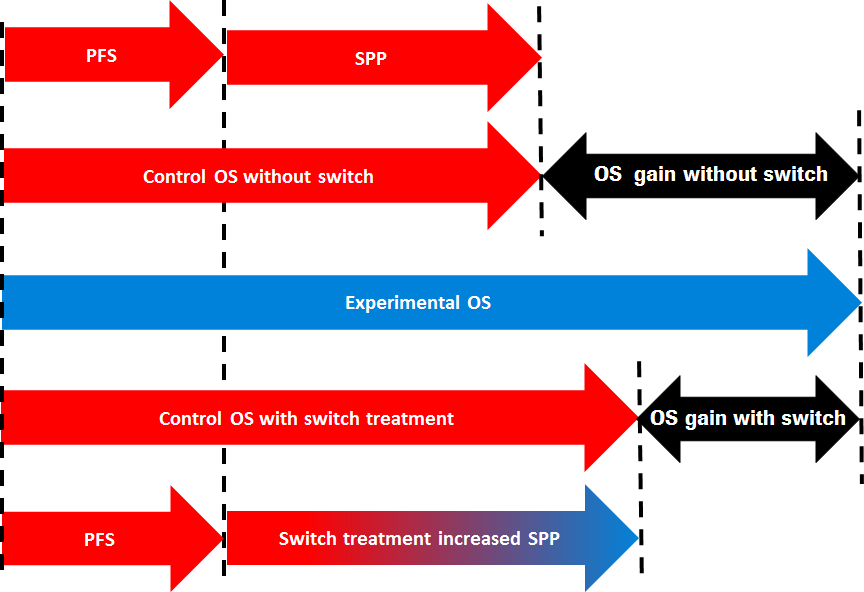
\includegraphics[width=14cm]{images/chap_intro/intro_pfsandpps.png}
\caption{\label{F:chap_intro:pfsandpps} Illustration of how treatment switching at progression can lead to contaminated estimates of overall survival. PFS = progression free survival, SPP = survival post progression, OS = overall survival. Adapted from \cite{Latimer2014}.} 
\end{figure}

\clearpage

\subsection{What is a true treatment effect?}
\label{S:chap_intro:whatest}
In this dissertation I will make commonly reference to a ``true'' or ``corrected'' treatment effect meaning the treatment effect that would have been observed if switching had not occurred. However, it will not always be the case that this ``corrected'' estimate is a useful estimate of treatment effect. For example it has been noted that if the observed treatment switch represents clinical practice no adjustment is necessarry as seen in \cite{PBAC2011} the PBAC assessment of erlotinib in Non-Small Cell Lung Cancer:
\begin{quote}
Because the EURTAC trial allowed for switching (cross-over) on disease progression, the results for overall survival inform a comparison of early versus late erlotinib; and they currently show no benefit (as at 26 January 2011 cut-off, log rank p = 0.8702).  The PBAC noted that the comparison of early versus late erlotinib is relevant in the Australian context because erlotinib is currently listed second-line in unselected patients.  Thus the clinical benefit for EGFR activating mutation positive patients of listing erlotinib as first-line treatment in addition to second-line treatment is an improvement in quality of life, but not a prolongation of life.
\end{quote}
In the event that the switch treatment does not represent clinical practice for instance if the experimental treatment is only available to both control and experimental arm patients through the clinical trial then  as noted by \cite{TSD16} ``[a comparison of randomised groups] is unlikely to be what is required [\ldots] because the ``true'' survival benefit associated with the novel intervention will be diluted due to the switching of control group patients onto the novel therapy.''  


\subsection{How does treatment switching affect interpretation?}
When considering the impact of treatment switching on the interpretation of a clinical trial it is important to consider the different questions that are being asked by stakeholders. A simplified overview of these is given below:
\begin{itemize}
\item FDA\footnote{United States Food and Drug Administration - United States Regulatory body.}, EMA\footnote{European Medicines Agency - European Regulator body.} - Benefit/Risk of an individual medicine   
\item IQWiG\footnote{Institute for Quality and Efficiency in Healthcare - Health Technology Assessment (HTA) body for Germany. } - Additional benefit compared to standard of care 
\item NICE\footnote{National Institute of Health and Care Excellence - HTA body for England and Wales.} - Additional benefit compared to standard of care extrapolated over patients life time  
\end{itemize}
In the case of considering benefit/risk of an individual medicine it is enough to show there is a treatment effect but the absolute magnitude of the effect is less important so long as it exceeds some minimum level. In this case what is important is the direction of bias with underestimation of treatment effect less concerning.

When making an assessment of benefit over standard of care it is necessary to estimate the magnitude of treatment effect with accuracy in order to enable comparisons to other therapies assuming that efficacy for these other therapies can be estimated accurately. Finally while it is not possible in this report to go into detail about methodological issues in performing an evaluation of treatment benefit extrapolated over lifetime it is sufficient to note that small changes in relative effect can translate into large differences in extrapolated absolute difference as illustrated in Figure \ref{F:chap_intro:extrapol}.

\begin{figure}[ht]
\centering
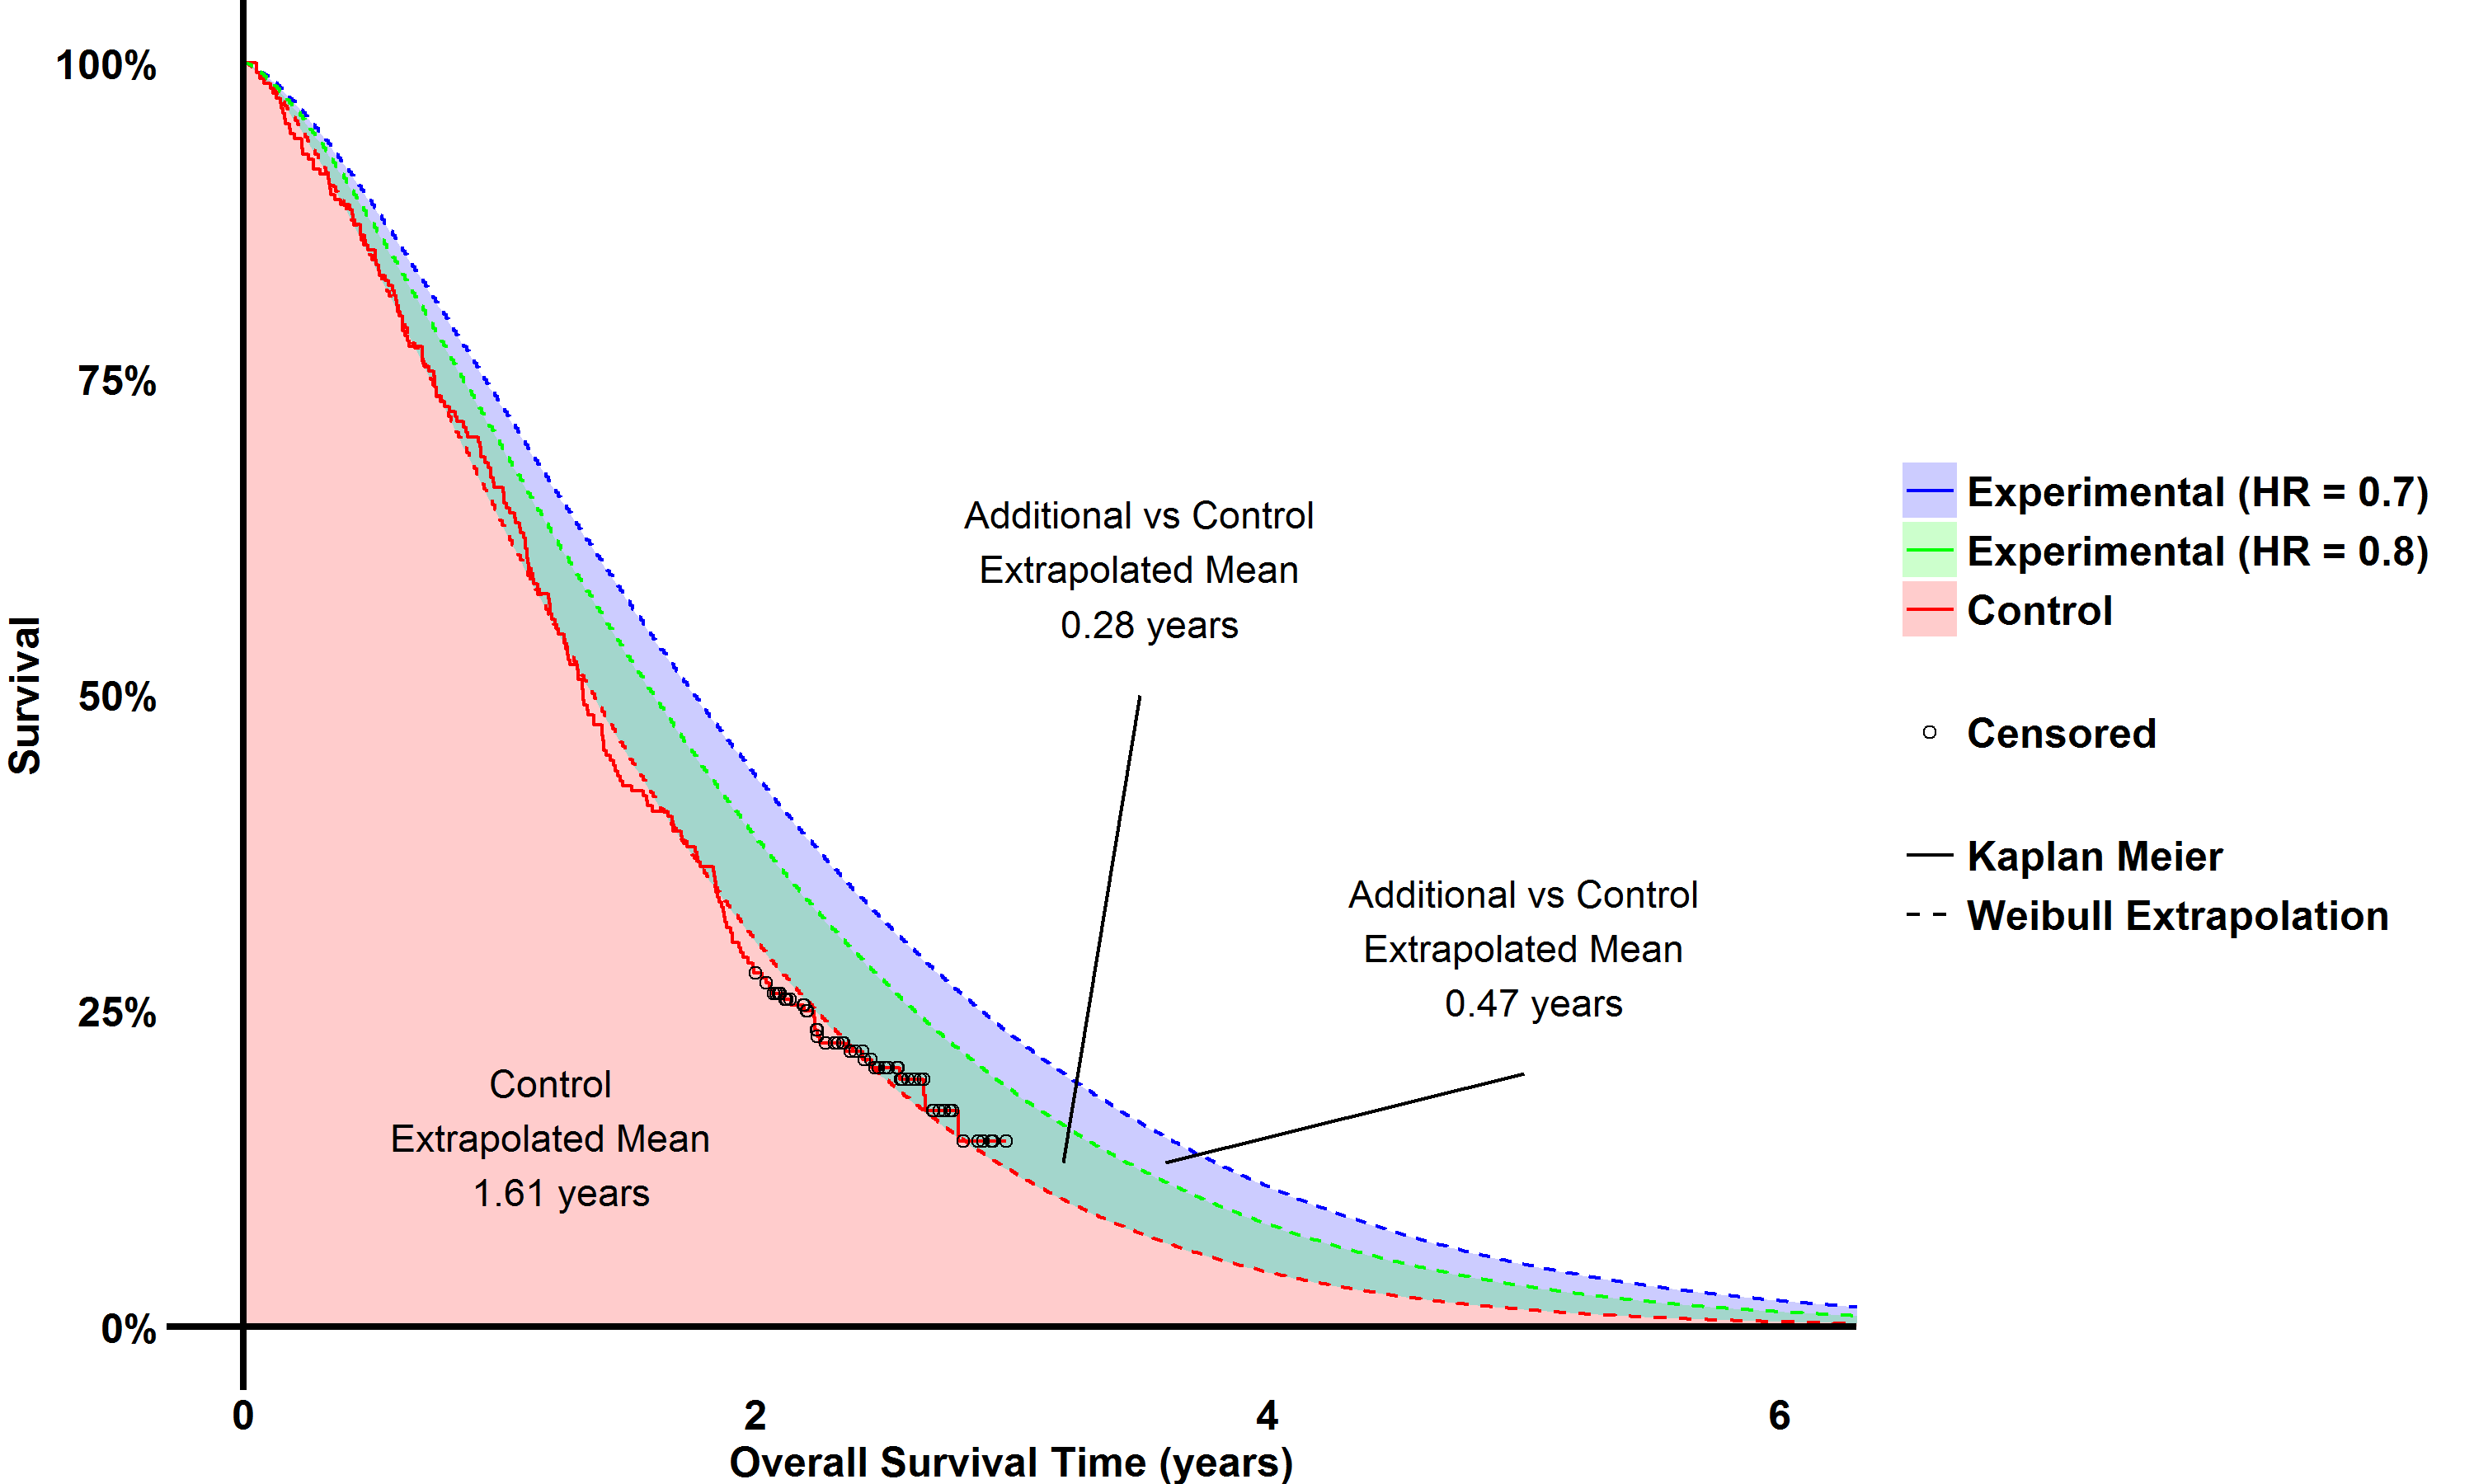
\includegraphics[width=14cm]{images/chap_intro/intro_extrapol.png}
\caption{\label{F:chap_intro:extrapol} Illustration of how quite small differences in the estimation of relative treatment effect can translate to important differences in absolute effects in the context of an economic evaluation. The mean life gain is estimated as the area under the extrapolated survival curve using the methods discussed in \cite{TSD14}.} 
\end{figure}

An additional important aspect here is to also consider the possibility of regulatory bodies accepting PFS as an endpoint to support approval of a medicine with \cite{TSD16} noting that ``showing an OS advantage may not be essential for obtaining marketing authorisation''. In these cases allowing switch at the time of progression only would not confound an analysis of PFS. However, there are clearly cases where OS benefit is required for regulatory approval such as TIVO-1 \cite{TIVO1} where there was no statistically significant difference in OS between the two arms, however, the point estimate for hazard ratio favoured the control arm:
\begin{quote}
This study met its primary end point by statistically significantly improving progression-free survival, but did impair overall survival, a secondary end point. Crossover from sorafenib to tivozanib may have confounded survival. Because of that detrimental survival, the US FDA rejected approval
\end{quote}
Though in this case it should be noted that \cite{Slaets2013} have performed simulation studies replicating this trial situation and found that it is unlikely that the absence of effect on overall survival was due to treatment switching alone.


\section{Use of simulation studies}
\label{S:chap_intro:simstudy}
In order to investigate the impact of treatment switching on the analysis of oncology trials I will use simulation studies. A simulation study is where a dataset such as a clinical trial are generated such that they have known true values for a parameter of interest to be estimated. Different statistical methods can then be used to analyse these datasets and the performance of these methods compared to the known truth. \cite{Burton2006} note that this is a common approach to assess the performance of statistical methods and advise that ``simulated data sets should have some resemblance to reality for the results to be generalizable to real situations and have any credibility''. 

In this case when considering clinical trials where multiple endpoints are measured from the same patient it is important to consider if these outcomes are correlated. In the context of treatment switching it is common for progression to be the trigger to switch from control to experimental therapy so any correlation between time to progression and overall survival could influence results. The explicit consideration of this correlation is the key difference between this work and prior simulation studies such as \cite{Morden2011}, \cite{Latimer2013} and \cite{Latimer2016}.

\subsection{Correlation between endpoints}
\label{S:chap_intro:correlation}

\cite{Ciani2014} have done a review of studies examining the correlation between progression free survival (PFS) and overall survival (OS). While this also considered studies that estimated correlations between treatment effects on these endpoints, of interest here is the correlation between PFS and OS for an individual patient. The results of the studies found that report an estimate of this correlation are reproduced in Table \ref{T:chap_intro:corr} adapted from Supplementary Table 2 of \cite{Ciani2014}. 


From Table \ref{T:chap_intro:corr} it can be seen that the estimate of correlation between PFS and OS varies both within and across different cancers. However, for the majority of the studies it is estimated to be $\ge 0.6$ and at the lowest is $0.3$ though this is for non-advanced/metastatic disease. This suggests that it is important to simulate data including correlations between these endpoints when assessing methods to adjust for overall survival. Though as will be discussed further in Section \ref{S:chap_sim_design:corr} progression free survival as a composite of time to progression and overall survival will be correlated with overall survival even if no correlation exists between time to progression and overall survival.

\begin{table}[hb] 
\caption{Reported correlations between progression free survival (PFS), time to progression (TTP) and overall survival (OS)}
\centering 
\begin{tabular}{|c|c|c|}

\multicolumn{3}{c}{Advanced Colorectal Cancer} \\
\hline
Outcome     & Estimate of Correlation    & Reference \\ 
            &  (95\% CI)    &           \\
\hline
PFS  & $R^2 = 0.61$ $(0.59 - 0.64)$  & \cite{Green2008}         \\ 
\hline
PFS  & $\rho = 0.82$ $(0.82 - 0.83)$  &  \cite{Buyse2007}       \\ 
\hline
PFS  & $\tau = 0.502$ $(0.457 - 0.548)$ &  \cite{Burzykowski2001}  (Method 1)   \\
\hline
PFS  & $\tau = 0.583$ $(0.548 - 0.619)$ &  \cite{Burzykowski2001} (Method 2) \\    
\hline    
\multicolumn{3}{c}{ } \\
\multicolumn{3}{c}{Advanced Ovarian Cancer}   \\
\hline
Outcome     & Estimate of Correlation    & Reference \\ 
            &  (95\% CI)    &           \\
\hline
 TTP  & $R^2 = 0.888$ (Not given) & \cite{Buyse2000}  \\    
\hline
PFS & $\tau = 0.857$ $(0.845 - 0.870)$ & \cite{Burzykowski2001} (Method 1)  \\    
\hline                        
PFS & $\tau = 0.839$ $(0.828 - 0.850)$ &  \cite{Burzykowski2001} (Method 2)\\        
\hline    
\multicolumn{3}{c}{ } \\
\multicolumn{3}{c}{Metastatic Breast Cancer}   \\
\hline
Outcome     & Estimate of Correlation    & Reference \\ 
            &  (95\% CI)    &           \\
\hline
PFS  & $\rho = 0.688$ $(0.686 - 0.690)$ & \cite{Burzykowski2008}   \\   
\hline     
TTP  & $\rho = 0.682$ $(0.682 - 0.684)$   & \cite{Burzykowski2008}   \\ 
\hline
\multicolumn{3}{c}{ } \\
\multicolumn{3}{c}{Progressive castrate-resistant prostate cancer }   \\
\hline
Outcome     & Estimate of Correlation    & Reference \\ 
            &  (95\% CI)    &           \\
\hline
PFS  & $\tau = 0.30$ $(0.26 - 0.32)$  & \cite{Halabi2009}   \\    
\hline
\multicolumn{3}{c}{ } \\
\multicolumn{3}{c}{Metastatic Renal Cell Carcinoma}   \\
\hline
Outcome     & Estimate of Correlation    & Reference \\ 
            &  (95\% CI)    &           \\
\hline
PFS  & $\tau = 0.42$  $(0.39 - 0.45)$  & \cite{Heng2010}   \\    
\hline
\end{tabular} 
\label{T:chap_intro:corr}
\end{table}





\chapter{Proposed Analysis Approaches}
\label{CHAP:methods}

A variety of methods have been proposed in the literature to analyse survival endpoints in clinical trials when treatment switching occurs. This chapter reviews the main methods proposed based primarily on those discussed within \cite{TSD16}. First considering those described as simple and then those described as complex. In this chapter I describe the analysis approaches, their key assumptions and some unclear aspects of implementation that will be investigated through simulation.

\section{Simple approaches}

\subsection{Intention-To-Treat (ITT) analysis}
Commonly in papers describing treatment switching reference is made to the ITT analysis. In the context of treatment switching this refers to analysing the trial results as observed and essentially ignoring that switching took place. If the experimental treatment is effective then this analysis could underestimate the true treatment effect. The magnitude of this bias will depend on the extent of the treatment switching both in terms of duration of exposure to switch treatment and proportion of patients exposed. 

\subsection{Per-protocol analysis}
Two similar approaches can be considered as per-protocol analysis as they exclude or censor data from patients who switch from the analysis. They both have the advantage that they are simple to implement in standard statistical software.

\subsubsection{Censoring at Crossover}
In this approach patients are censored at the time they switch treatment. The key assumption made is that this censoring is non-informative meaning that the outcome being analysed is independent of the switching. \cite{TSD16} challenge this assumption stating that ``clinicians decide whether it is appropriate for individual patients to switch and this decision will be made based upon patient characteristics rather than being random''. 

\subsubsection{Excluding Switchers}
For this analysis patients who switch are excluded from the analysis. This breaks the randomization and as \cite{Watkins2013} note ``makes the assumption that the control arm switchers and non-switchers have the same prognosis'' which as noted previously is an assumption that \cite{TSD16} challenge. \cite{Watkins2013} also highlight that ``Patients also have to live long enough to be able to switch, so longer-living individuals are removed.'' further creating the potential for bias to be introduced into the analysis.

\subsection{Time-dependent Cox proportional hazards model}

A further approach is to include treatment exposure as a time varying covariate into a Time dependent Cox-model. Such models can be easily fit with standard statistical software. However, while easy to implement \cite{Watkins2013} note this approach will be biased ``If there are confounding variables that influence both the time-varying treatment covariate and survival.'' While in a non-oncology setting \cite{Hernan2000} are explicit that:
\begin{quote}
[the time-dependent Cox proportional hazards model] approach may be biased, whether or not one further adjusts for past covariate history, whenever (1) there exists a time-dependent covariate that is both a risk factor for mortality and also predicts subsequent exposure and (2) past exposure history predicts the risk factor.
\end{quote}
In the context of oncology clinical trials \cite{TSD16} state that it is highly likely that ``switching is associated with prognostic patient characteristics''. It is clear that such prognostic patient characteristics would be confounding variables by this definition and therefore the time varying covariate analysis may be biased even if adjusted for these characteristics.

A potential variation of this approach that may address these limitations is where two covariates are considered for treatment: one for randomized treatment that is not time dependent and a second covariate for exposure to experimental therapy as a switch therapy that is time dependent as described by \cite{Leon2014}. 

\section{Inverse Probability of censoring Weights (IPCW)}

The analysis method or IPCW described by \cite{Robins2000} censors information that occurs after treatment switch. In order to avoid the selection bias that can confound the per-protocol analysis of censoring at treatment switch observations that are not censored are weighted to create a pseudopopulation with the same characteristics as the overall trial population. To do this a model is built to predict censoring based on observed covariates over time which is used to estimate for each patient the conditional probability of remaining uncensored. The inverse of this estimated probability is then used as a weight into the estimation of a corrected hazard ratio. 

\subsection{Model for censoring}

The model for censoring can be in either discrete or continuous time. The primary benefit of using discrete time is the ease of calculation in standard software such as the demonstrations by \cite{Hernan2000} or \cite{Fewell2004}. In the case of discrete time the model for probability of censoring is of the form shown in Equation \ref{E:chap_methrev:IPCWcm}. Where $\mathbb{P}(C=1|t)$ indicates the probability of being censored in interval $t$, with $t=0,1, \ldots, T$ representing discrete time intervals, $X_t$ is a vector of time dependent covariates and $X_0$ is a vector of baseline covariates and the $\beta$ terms can be estimated through e.g. pooled logistic regression including each patient multiple times.

\begin{equation}
\label{E:chap_methrev:IPCWcm}
\mathbb{P}(C=1|t) = \alpha_t + \beta_0^\prime  X_0 + \beta^\prime X_t 
\end{equation}

It can be seen that this model requires covariates ($X_t$) for each patient for all time periods until censoring (or death). While for patients who switch this may be feasible for patients who do not switch it is unclear if this feasible. In practice it may be necessary to replace the covariate values by predicted values from a mixed effect repeated measures model of the covariate over time (making additional assumptions about any missingness).

\subsection{Estimating the weights}

By multiplying the probability of being uncensored in each time period the cumulative probability of being uncensored at each time for each patient can be estimated. For unstabilized weights the inverse of this probability is taken while for stabilized weights the same process is used but instead of the numerator being 1 the numerator is based on the probability of being uncensored given only baseline covariates. As such the formula for unstabilized weights is shown in Equation \ref{E:chap_methrev:IPCW.W} and for stabilized weights in Equation \ref{E:chap_methrev:IPCW.SW}. 

\begin{equation}
\label{E:chap_methrev:IPCW.W}
\hat{W}(t) = \prod^t_{k=0} \frac{1}{1-\mathbb{P}(C=1|k, X_0, X_k)}
\end{equation}

\begin{equation}
\label{E:chap_methrev:IPCW.SW}
\hat{W}(t) = \prod^t_{k=0} \frac{1-\mathbb{P}(C=1|k, X_0)}{1-\mathbb{P}(C=1|k, X_0, X_k)}
\end{equation}

\subsection{Model requirements}

\cite{Cole2008} identifies the key requirements for this model to yield valid estimates as Exchangeability and Positivity. Exchangability simply means that all covariates that influence censoring and outcome are captured in the weight estimation model and that given these covariates over time any given patient is exchangeable with another having the same covariate history. This is commonly referred to as the no unmeasured confounders assumption by \cite{TSD16} and others. The second requirement of Positivity is defined by \cite{Cole2008} as ``the condition that there are both exposed and unexposed individuals at every level of the confounders.''. It can be seen that these two conditions can be in conflict particularly in the presence of small sample sizes (such as a clinical trial) whereby each additional covariate introduced to improve the exchangeability assumption will increase the possibility of creating a level of covariates for which the probability of being censored is 0 or 1 violating the positivity assumption. This issue has been shown in practice in the simulation study of \cite{Latimer2013} where scenarios with very high switching proportions lad to large bias as no patients existed to replace those who switched.

\subsection{Estimating a corrected Hazard Ratio}

After weights by patient and time have been estimated it is possible to include them into a time dependent weighted Cox model driectly or into a weighted generalized linear model using a complementary log-log link to estimate a hazard ratio as shown by \cite{Hernan2000}. In this model patients who switch treatment are censored at the time of switch.

\section{Rank Preserving Structural Failure Time (RPSFT) models}

\cite{Robins1991} introduced a randomization based approach to address treatment non-compliance in clinical trials. It considers 3 different survival times for a patient $i$:
\begin{enumerate}
\item $T_i$ which is their observed survival time given their observed treatment history
\item $U_i$ which is their ``latent'' survival time  under no treatment. This is an unobserved baseline variable.
\item $V_i$ which is their ``counter-factual'' survival time under some different treatment history than that observed. 
\end{enumerate}
An RPSFT model is then defined to relate these survival times and enable the estimation of $V_i$. 

\subsection{The RPSFT model}
The general form of the RPSFT model is shown in Equation \ref{E:rpsft1}. Here I deviate from the notation used by \cite{Robins1991} where they define a model $\psi()$ with parameters $\beta$ wheras I follow here the convention commonly in later papers e.g. \cite{White1999}, \cite{Morden2011} or \cite{Watkins2013} to use $\psi$ to refer to the parameters of the model.  
\begin{equation}
\label{E:rpsft1}
U_i = f\left(T_i, H_i(T_i), \psi \right)
\end{equation}
$H_i()$ is a time dependent treatment history which for $H_i(T_i)$ is observed and $\psi \in \mathrm{R}^v, v \geq 1$ are unknown parameters. $f()$, the RPSFT model, is then a smooth function which satisfies the following criteria:
\begin{enumerate}
\item It is rank preserving so that $u_a = f(t_a,H_i(t_a),\psi) > u_b = f(t_b,H_i(t_b),\psi)$ if $t_a>t_b$ which means that if a patient $a$ with longer survival than $b$ with the same treatment history would also have longer survival when both had any other treatment history.
\item $t=f(t,H_i(t),\psi)$ if $H_i(t)$ is identically 0 on $(0,t)$ so without treatment the latent survival time is observed.
\item $t=f(t,H_i(t),0)$ so $\psi$ identically 0 implies no treatment effect.
\end{enumerate}
Given such a model $f$ where the parameters $\psi$ are known it is possible to estimate the latent survival times $U_i$ form the observed survival time $T_i$ and observed treatment history $H_i(T_i)$. These latent survival times can then be used to estimate $V_i^{(h)}$ the counter-factual survival times under another treatment history $(h)$. In the context of treatment switching this counter-factual treatment history would normally be where patients took only their randomized treatment. Equation \ref{E:rpsft2} shows this relationship. It is important to note that $V_i^{(h)}$ depends only on $U_i$ and not $T_i$ which will be considered further when discussing issues with censored data.
\begin{equation}
\label{E:rpsft2}
U_i = f\left(V_i^{(h)}, H^{(h)}_i(V_i^{(h)}),\psi\right)
\end{equation}

\subsubsection{Model assumptions}
Two key assumptions are made with this method. The first assumption is that the distribution of $U_i$ the latent survival time will be balanced by randomization between the randomized groups of the trial as it is a baseline characteristic. \cite{TSD16} notes that this assumption ``should be reasonable in the context of an RCT'' and that while important differences could occur in trials this maybe addressed through adjusting for prognostic covariates. The second assumption is that the RPSFT model chosen is correct. The specific form of the model chosen will therefore create its own assumptions.



\subsection{Model fitting}
Once the structural model relating $U$ and $T$ has been defined it is necessary to estimate the unknown parameters $\psi$. This is estimated through a process known as g-estimation. \cite{Robins1991} rely on the assumption that latent survival is balanced through randomization and use rank tests of the hypothesis that the $U_i$ are independent of randomized arm to define $\psi_0$ as the value where this hypothesis is true. \cite{KorhonenATBC}, \cite{White1999} and others describe the processes to get an estimate $\hat{\psi}$ of $\psi_0$ as follows.

\begin{enumerate}
\item Define a grid of candidate values for $\psi$.
\item For each $\psi$ estimate the latent survival time $U(\psi)$.
\item Compare the latent survival times as randomized with a suitable test (commonly a log-rank test) to get a test-statistic, $Z(U,\psi) = Z(\psi)$, for the difference in distributions of the $U$ comparing the control and experimental arms.
\item Choose $\hat{\psi}$ such that $Z(\hat{\psi}) \simeq Z(\psi_0)$, that is choose $\hat{\psi}$ such that the distribution of $U$ in the control arm is close to that of the distribution of $U$ in the experimental arm, ``the point estimate $\hat{\psi}$ is taken as the value closest to the null value where the test statistic reaches its minimum (or equivalently the p-value is at its maximum)'' \citep{KorhonenRECORD}. 
\end{enumerate}

This is illustrated in Figure \ref{F:C2:demo_g_est} for a simulated data set.
\begin{figure}[ht]
\centering
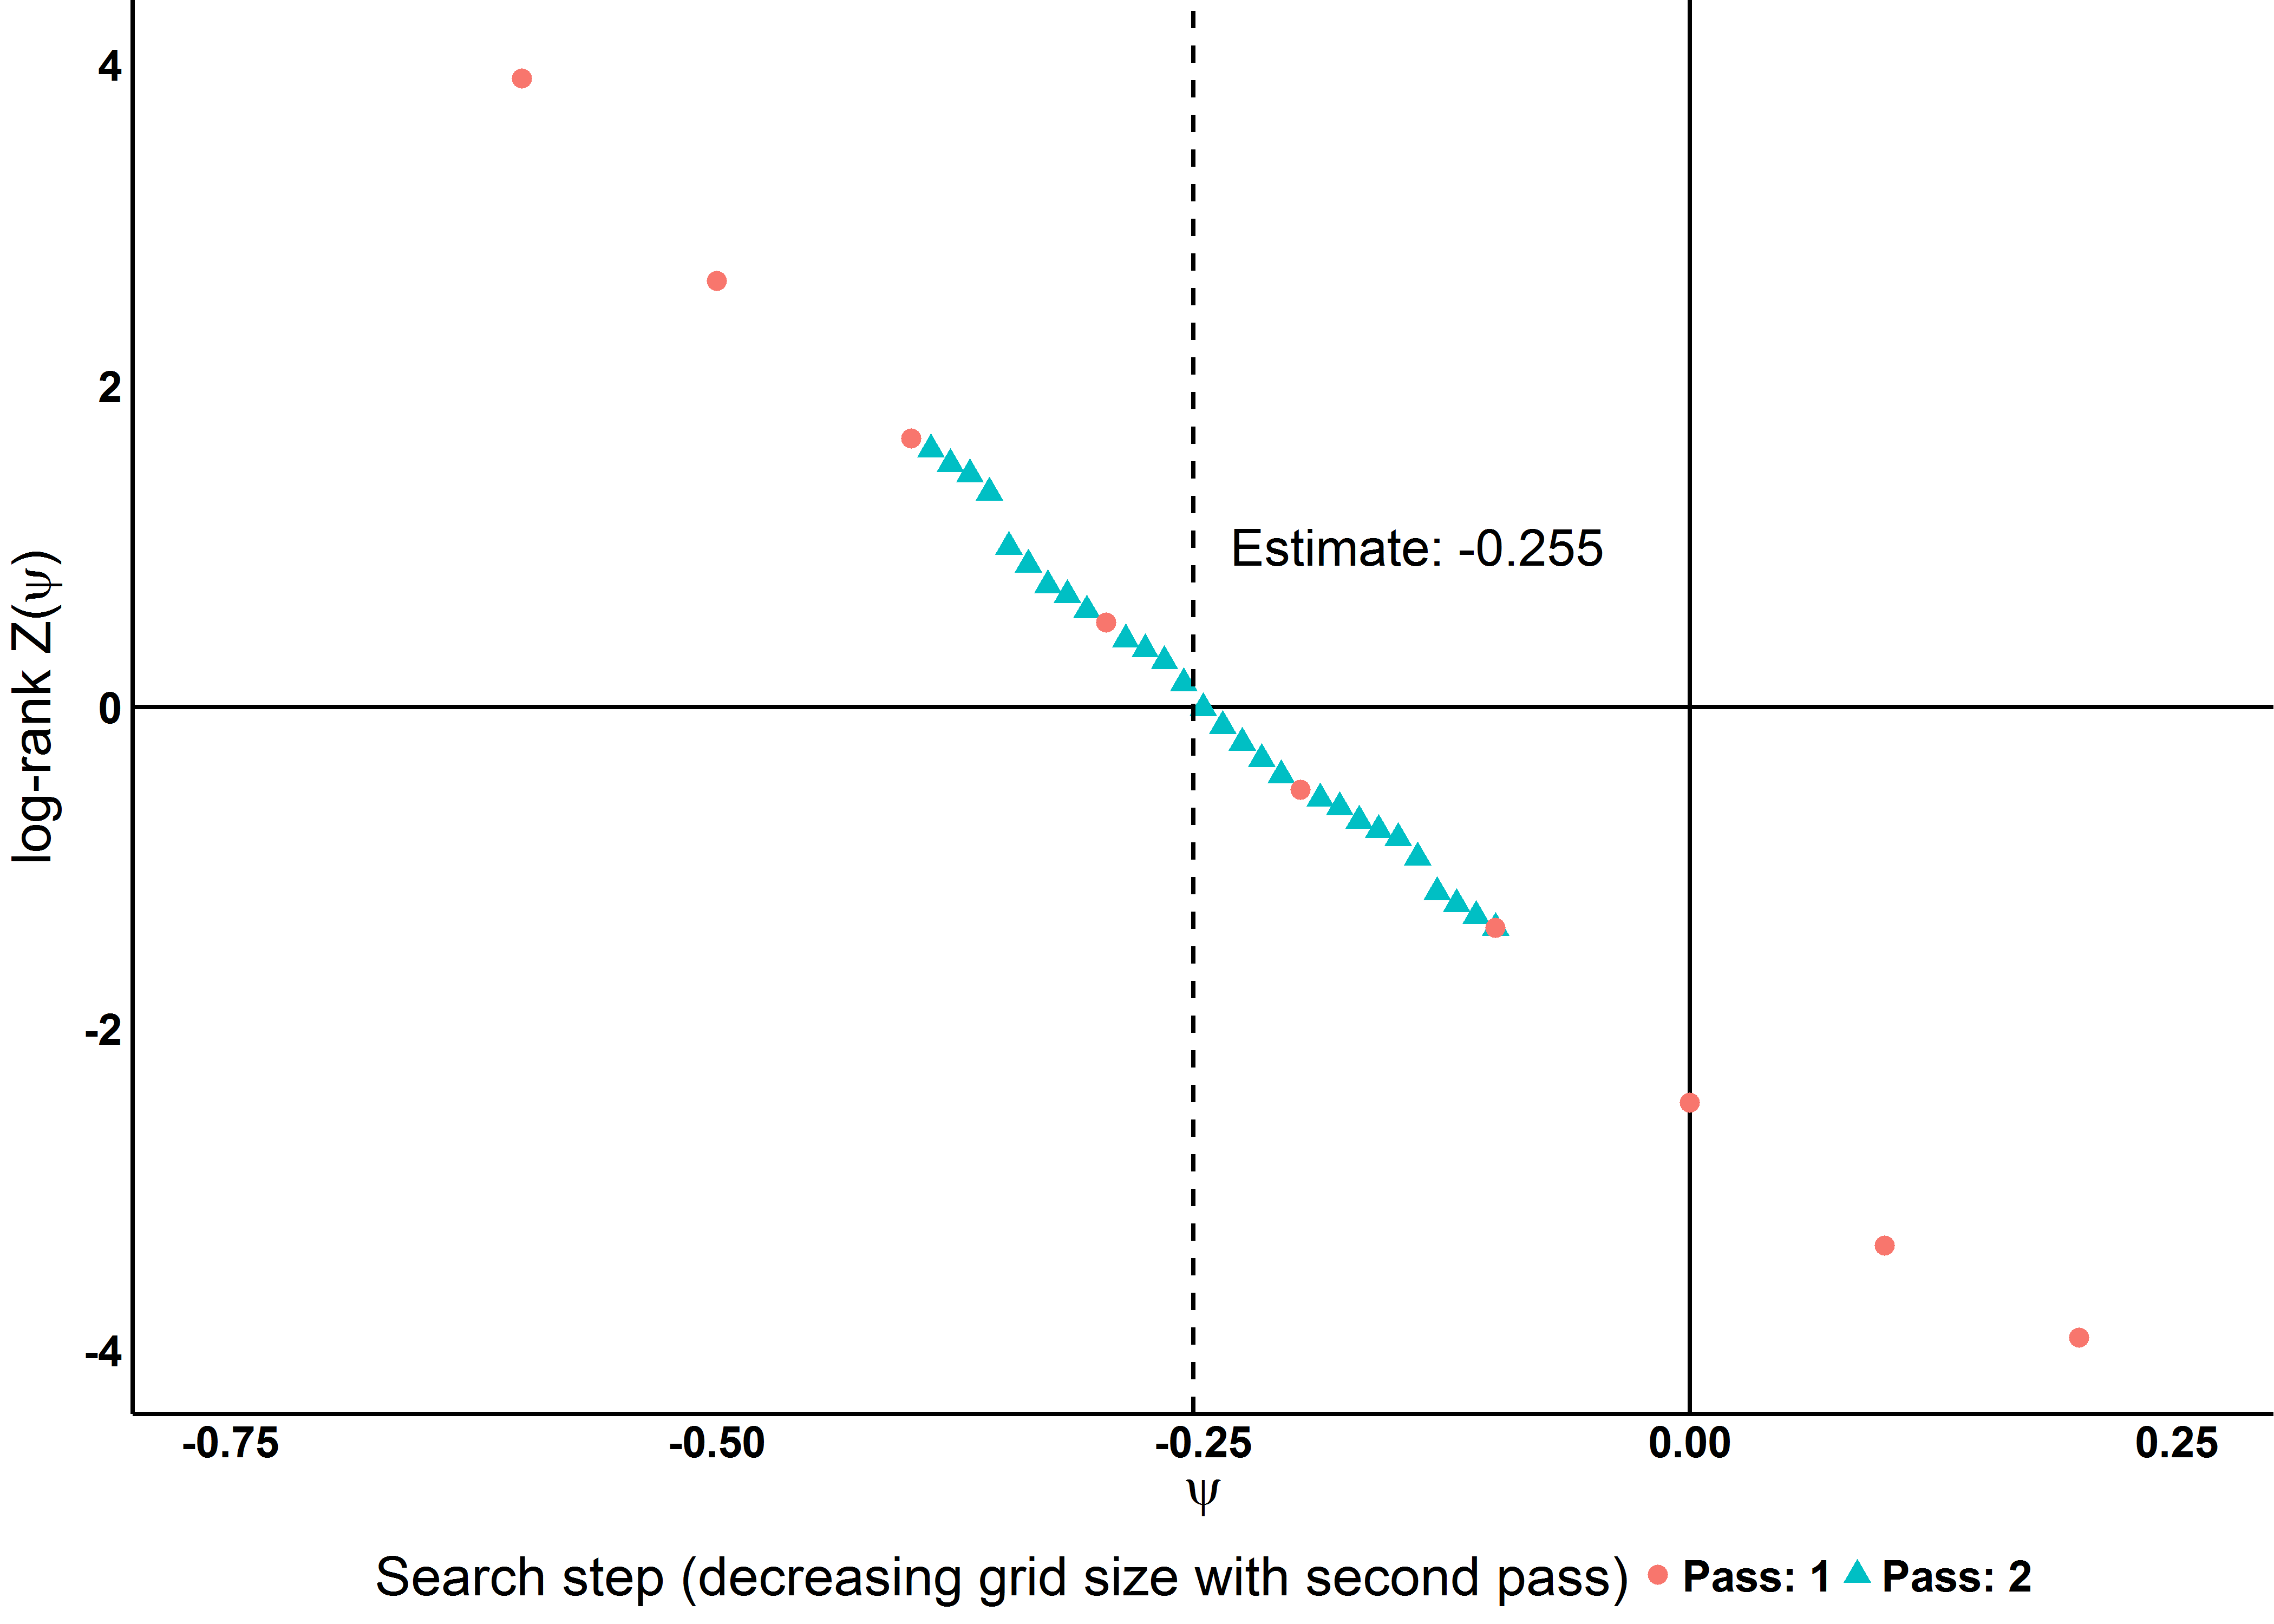
\includegraphics[width=13cm]{images/chap_methrev/example_g_est.png}
\caption{\label{F:C2:demo_g_est} Illustration of g-estimation using log-rank test statistic with $\hat{\psi}$ estimated as -0.255.} 
\end{figure}

\label{S:chap_methrev:RPSFTfit}

\subsubsection{Choice of test}

\cite{Robins1991} note for all datasets a locally most powerful test with a unique solution will exist, however, identifying this test is not trivial. \cite{TSD16} states that ``a log-rank or Wilcoxon test can be used for the RPSFTM g-test in a non-parametric setting [\ldots] or a Wald test could be used for parametric models''. In a non-parametric setting \cite{KorhonenRECORD} investigated the Fleming-Harrington family of rank tests which have a parameter $\rho$ and includes both log-rank ($\rho=0$) and Wilcoxon ($\rho=1$) tests and found that for their application ``[$\hat{\psi}$] is quite robust to different values of $\rho$''. 

\subsubsection{Issues with estimation}

\label{S:chap_methrev:ESTissues}
\cite{White1999} and \cite{White2002} identified a challenge in the g-estimation of $\hat{\psi}$ that as a rank test is used there may not be a solution where $Z(\psi)=0$.  Their proposed solution is to interpolate between the points where the sign of $Z(\psi)$ changes. It should be noted this is only possible when considering a test statistic that indicates a direction for the difference in survival times comparing the $U_i$ as randomized. As an example considering the log-rank test this means it is preferable to perform the g-estimation using the log-rank test statistic directly rather than use the $\chi^2$ value or $p$-value from the test. in addition they recommend an approach to take if multiple such crossing points are found:
\begin{quote}
We obtained a single point estimate $\hat{\psi}$ as follows. If the crossing points are $a_0$, $a_1$, $a_2$, \ldots, $a_n$ (where $n$ is even), then we took $\hat{\psi} = a_0 -a_1+a_2-\ldots+a_n$. This can be viewed as an average of the extreme crossing points $a_0$ and $a_n$, weighted by the length of time for which $Z(\psi)$ is positive and negative for $\psi$ in [$a_0$, $a_n$]
\end{quote}


\subsubsection{Handling Censored Data}
\cite{Robins1991} identified that non-informative censoring on the observed ($T$) time scale may become informative on the latent survival ($U$) time scale. To illustrate this problem I adapt the explanation of \cite{KorhonenRECORD} using the one-parameter ``treatment group'' approach as shown in Equation \ref{E:rpsftm3b}. To begin consider a trial of a experimental therapy which is beneficial and doubles life ($e^\psi=0.5$). Then consider two patients who the same latent survival time of 3 months ($U_1=U_2=3$). If patient $1$ is randomized to control but receives 1 month of experimental therapy then $T_1=2+\frac{1}{e^\psi}=4$ while if patient $2$ is randomized to the experimental arm then $T_2=0+\frac{3}{e^\psi}=6$. If the trial was completed at 6 months then we would observe both patients events and able to recover the unobserved $U_i$ using Equation \ref{E:rpsftm3b}. However, if the trial was completed at 4 months we would still observe $T_1=4$ but would only know that $T_2>4$. Just applying Equation \ref{E:rpsftm3b} would lead us to state that $\hat{U_1}=3$ and that $\hat{U_2}>2$ showing that censoring is not independent of randomization on the latent survival time scale.


\cite{Robins1991} note the solution is simple when considering administrative censoring where a potential censoring time $C_i$ is known for each patient. Then it is just necessary to re-censor the $U_i$ at a time at that is ``less then of equal to the earliest time on the [estimated latent survival] time-scale that any subject with potential censoring time $C$ could have been censored.'' \cite{White1999} proposes a simple, but potentially conservative, approach which is to assume that under a different treatment history a patient could have been never treated or always treated leading to a censoring time $C_i^\star$ on the latent survival time scale as shown in Equation \ref{E:rpsftcens}.
\begin{equation}
\label{E:rpsftcens}
C_i^\star(\psi) = \min \left( C_i, C_i e^\psi \right)
\end{equation}


While this approach is only strictly valid for adminstrative censoring at the end of the study \cite{White2002} notes that ``if small amounts of random censoring are present, a reasonable approximation is to set the potential censoring time for subjects who are randomly censored equal to the actual time of random censoring.''





\subsection{The one-parameter model}
\label{S:chap_methrev:RPSFTonep}
A commonly used model described by \cite{Watkins2013} and others is to consider $\psi$ to be one dimensional and that $H(t)$ indicates exposure to experimental treatment. This is shown in Equations \ref{E:rpsftm1a} and \ref{E:rpsftm1b} where $T_{Ei}$ is the time a patient is exposed to Experimental therapy and $T_{Ci} = T_i - T_{Ei}$.
\begin{align}
U_i =& f\left(T_i, H_i(T_i), \psi\right) = \int_0^{T_i} \exp\left(\psi H_i(s) \right) ds \label{E:rpsftm1a}\\
H_i(t)=& \begin{cases} 
	0 &,t \in T_{Ci} \\ 
    1 &,t \in T_{Ei} 
    \end{cases}  \label{E:rpsftm1b}
\end{align}
\cite{TSD16} describe two ways of constructing $t_{Ei}$ that they describe as ``on treatment'' and ``treatment group'' approaches. To compare these it is helpful to define for each patient a start and stop time for experimental therapy as $A_{i}$ and $B_{i}$. 

\subsubsection{``on treatment'' approach}
With this approach the time actually on experimental treatment is used to define $T_{Ei} = B_{i} - A_{i}$ so $H_i$ and $U_i$ can be defined as shown in  Equations \ref{E:rpsftm2a} and \ref{E:rpsftm2b}.
\begin{align}
H_i(t)=& \begin{cases} 
	0 &, 0 \leq t < A_{i} \\ 
    1 &, A_{i} \leq t  \leq B_{i} \\
    0 &, B_{i} < t  \leq T_i
    \end{cases}  \label{E:rpsftm2a}\\
U_i =& \int_0^{T_i} \exp\left(\psi H_i(s) \right) ds \nonumber  \\
    =& \int_0^{A_i} \exp\left(\psi 0 \right) ds + \int_{A_i}^{B_i} \exp\left(\psi 1 \right) ds + \int_{B_i}^{T_i} \exp\left(\psi 0 \right) ds  \nonumber \\
    =& A_i + (B_i-A_i)e^{\psi} + (T_i - B_i) \nonumber \\
    =& (T_i - (B_i - A_i)) + (B_i-A_i)e^{\psi}  \label{E:rpsftm2b}
\end{align}

\subsubsection{``treatment group'' approach}
With this approach the time from the start of experimental treatment is used to define $T_{Ei} = T_{i} - A_{i}$ so $H_i$ and $U_i$ can be defined as shown in  Equations \ref{E:rpsftm3a} and \ref{E:rpsftm3b}.
\begin{align}
H_i(t)=& \begin{cases} 
	0 &, 0 \leq t < A_{i} \\ 
    1 &, A_{i} \leq t  \leq T_{i} 
    \end{cases}  \label{E:rpsftm3a}\\
U_i =& \int_0^{T_i} \exp\left(\psi H_i(s) \right) ds \nonumber  \\
    =& \int_0^{A_i} \exp\left(\psi 0 \right) ds + \int_{A_i}^{T_i} \exp\left(\psi 1 \right) ds  \nonumber \\
    =& A_i + (T_i-A_i)e^{\psi}  \label{E:rpsftm3b}
\end{align}

\subsubsection{Interpretation of the one-parameter model}
By rearranging Equation \ref{E:rpsftm3b} it can be seen that $T_i = A_i + (U_i-A_i)e^{-\psi}$ and that $e^{-\psi}$ can be interpreted as an Acceleration Factor within an Accelerated Failure Time (AFT) model. It can be seen that when $\psi < 0$ then $e^{-\psi} > 1$ implying that exposure to experimental treatment is beneficial and extends latent survival time. It can also be seen that that for this model the benefit of treatment doesn't depend on when the treatment is received but only the duration and the implicit assumption is made that the experimental treatment is equally beneficial first-line in the experimantal arm as it is second-line in the control arm. This is referred to as the ``common treatment effect'' assumption by \cite{TSD16}, \cite{Watkins2013} and others. 

\subsection{A two-parameter model}
 An obvious method to address the limitations of the ``common treatment effect'' assumption would be to define a two-parameter model where first and second line treatment are allowed to have different effects. Using similar notation to the one-parameter model use $T_{E1i}$ and $T_{E2i}$ to denote the duration of first and second line therapy respectively with $T_{Ci}$ the duration of control therapy so define the model as shown in Equations \ref{E:rpsftm4a} and \ref{E:rpsftm4b}.
 
 \begin{align}
 H_{1i}(t)=& \begin{cases}        
	0 &, t \not\in T_{E1i} \\ 
    1 &, t \in T_{E1i}
    \end{cases}                
    &  
 H_{2i}(t)=& \begin{cases}        
	0 &, \not\in T_{E2i} \\ 
    1 &, t \in T_{E2i}
    \end{cases}                
                \label{E:rpsftm4a}
\end{align}                
\begin{align}
U_i =& \int_0^{T_i} \exp\left(\psi_1 H_{1i}(s) + \psi_2 H_{2i}(s) \right) ds \nonumber  \\
    =& T_{Ci} + T_{E1i} e^{\psi_1} + T_{E2i} e^{\psi_2} \label{E:rpsftm4b}
\end{align}

However, while simple to define \cite{White1999} describes the challenges of g-estimation in two-dimensions specifically that ``To estimate two parameters, two tests of the equality of $U$ across the two arms are required.'' which leads to very large confidence regions for the parameters. Because of this difficulty these models have not been widely used with \cite{TSD16} noting that ``analysts have attempted to apply a multiparameter version of the RPSFTM. However these have not been successful, with meaningful point estimates for causal effects difficult to determine.'' 

Given the challenges in estimating multiple parameters \cite{White2014} has proposed instead a sensitivity analysis for this by defining $\psi_2 = k\psi_1$ where $k$ is a known value chosen to represent second line therapy being fractionally as effective as first line therapy. The model is then fit for a range of $k$ where 0 represents no effect second line while 1 represents an equal effect to first line.

\subsection{Estimating a corrected Hazard Ratio}
\label{S:chap_methrev:RPSFTestHR}

Once $\hat{\psi}$ has been estimated counter-factual survival times $V_i$ can be estimated for all patients for any desired treatment history. In the context of treatment switching in oncology trials using the ``treatment group'' approach the desired counter-factual treatment history would be for patients randomized to the control arm to never receive experimental therapy. There are two possible approaches to derive such counter-factual times for this model. The first is to simply set $V_i=T_i$ for the experimental arm and $V_i=U_i$ for the control arm as suggested by \cite{Latimer2014}. The second is to follow the approach of \cite{Robins1991} and derive the $V_i$ from $U_i$ by solving Equation \ref{E:rpsft2} for each treatment history. In this case solving Equation \ref{E:rpsftm3b} have $U_i = V_i + (V_i - V_i)e^\psi \Rightarrow V_i = U_i$ for the control arm and $U_i = 0 + (V_i - 0)e^\psi \Rightarrow V_i = e^-\psi U_i$ for the experimental arm. 


For the control arm nothing changes and for the the ``treatment group'' model the experimental arm estimates do not change under the assumption of only administrative censoring (as can be seen by considering Equation \ref{E:rpsftcens}). However, for the ``on treatment'' approach when censoring occurs the counterfactual survival times for the experimental arm derived from the latent survival times may not match the observed experimental survival times. This can be seen in Figure \ref{F:methrev:excfact}. It is unclear what if any bias is introduced by the simple approach compared to the counter-factual only approach. 

\begin{figure}[ht]
\centering
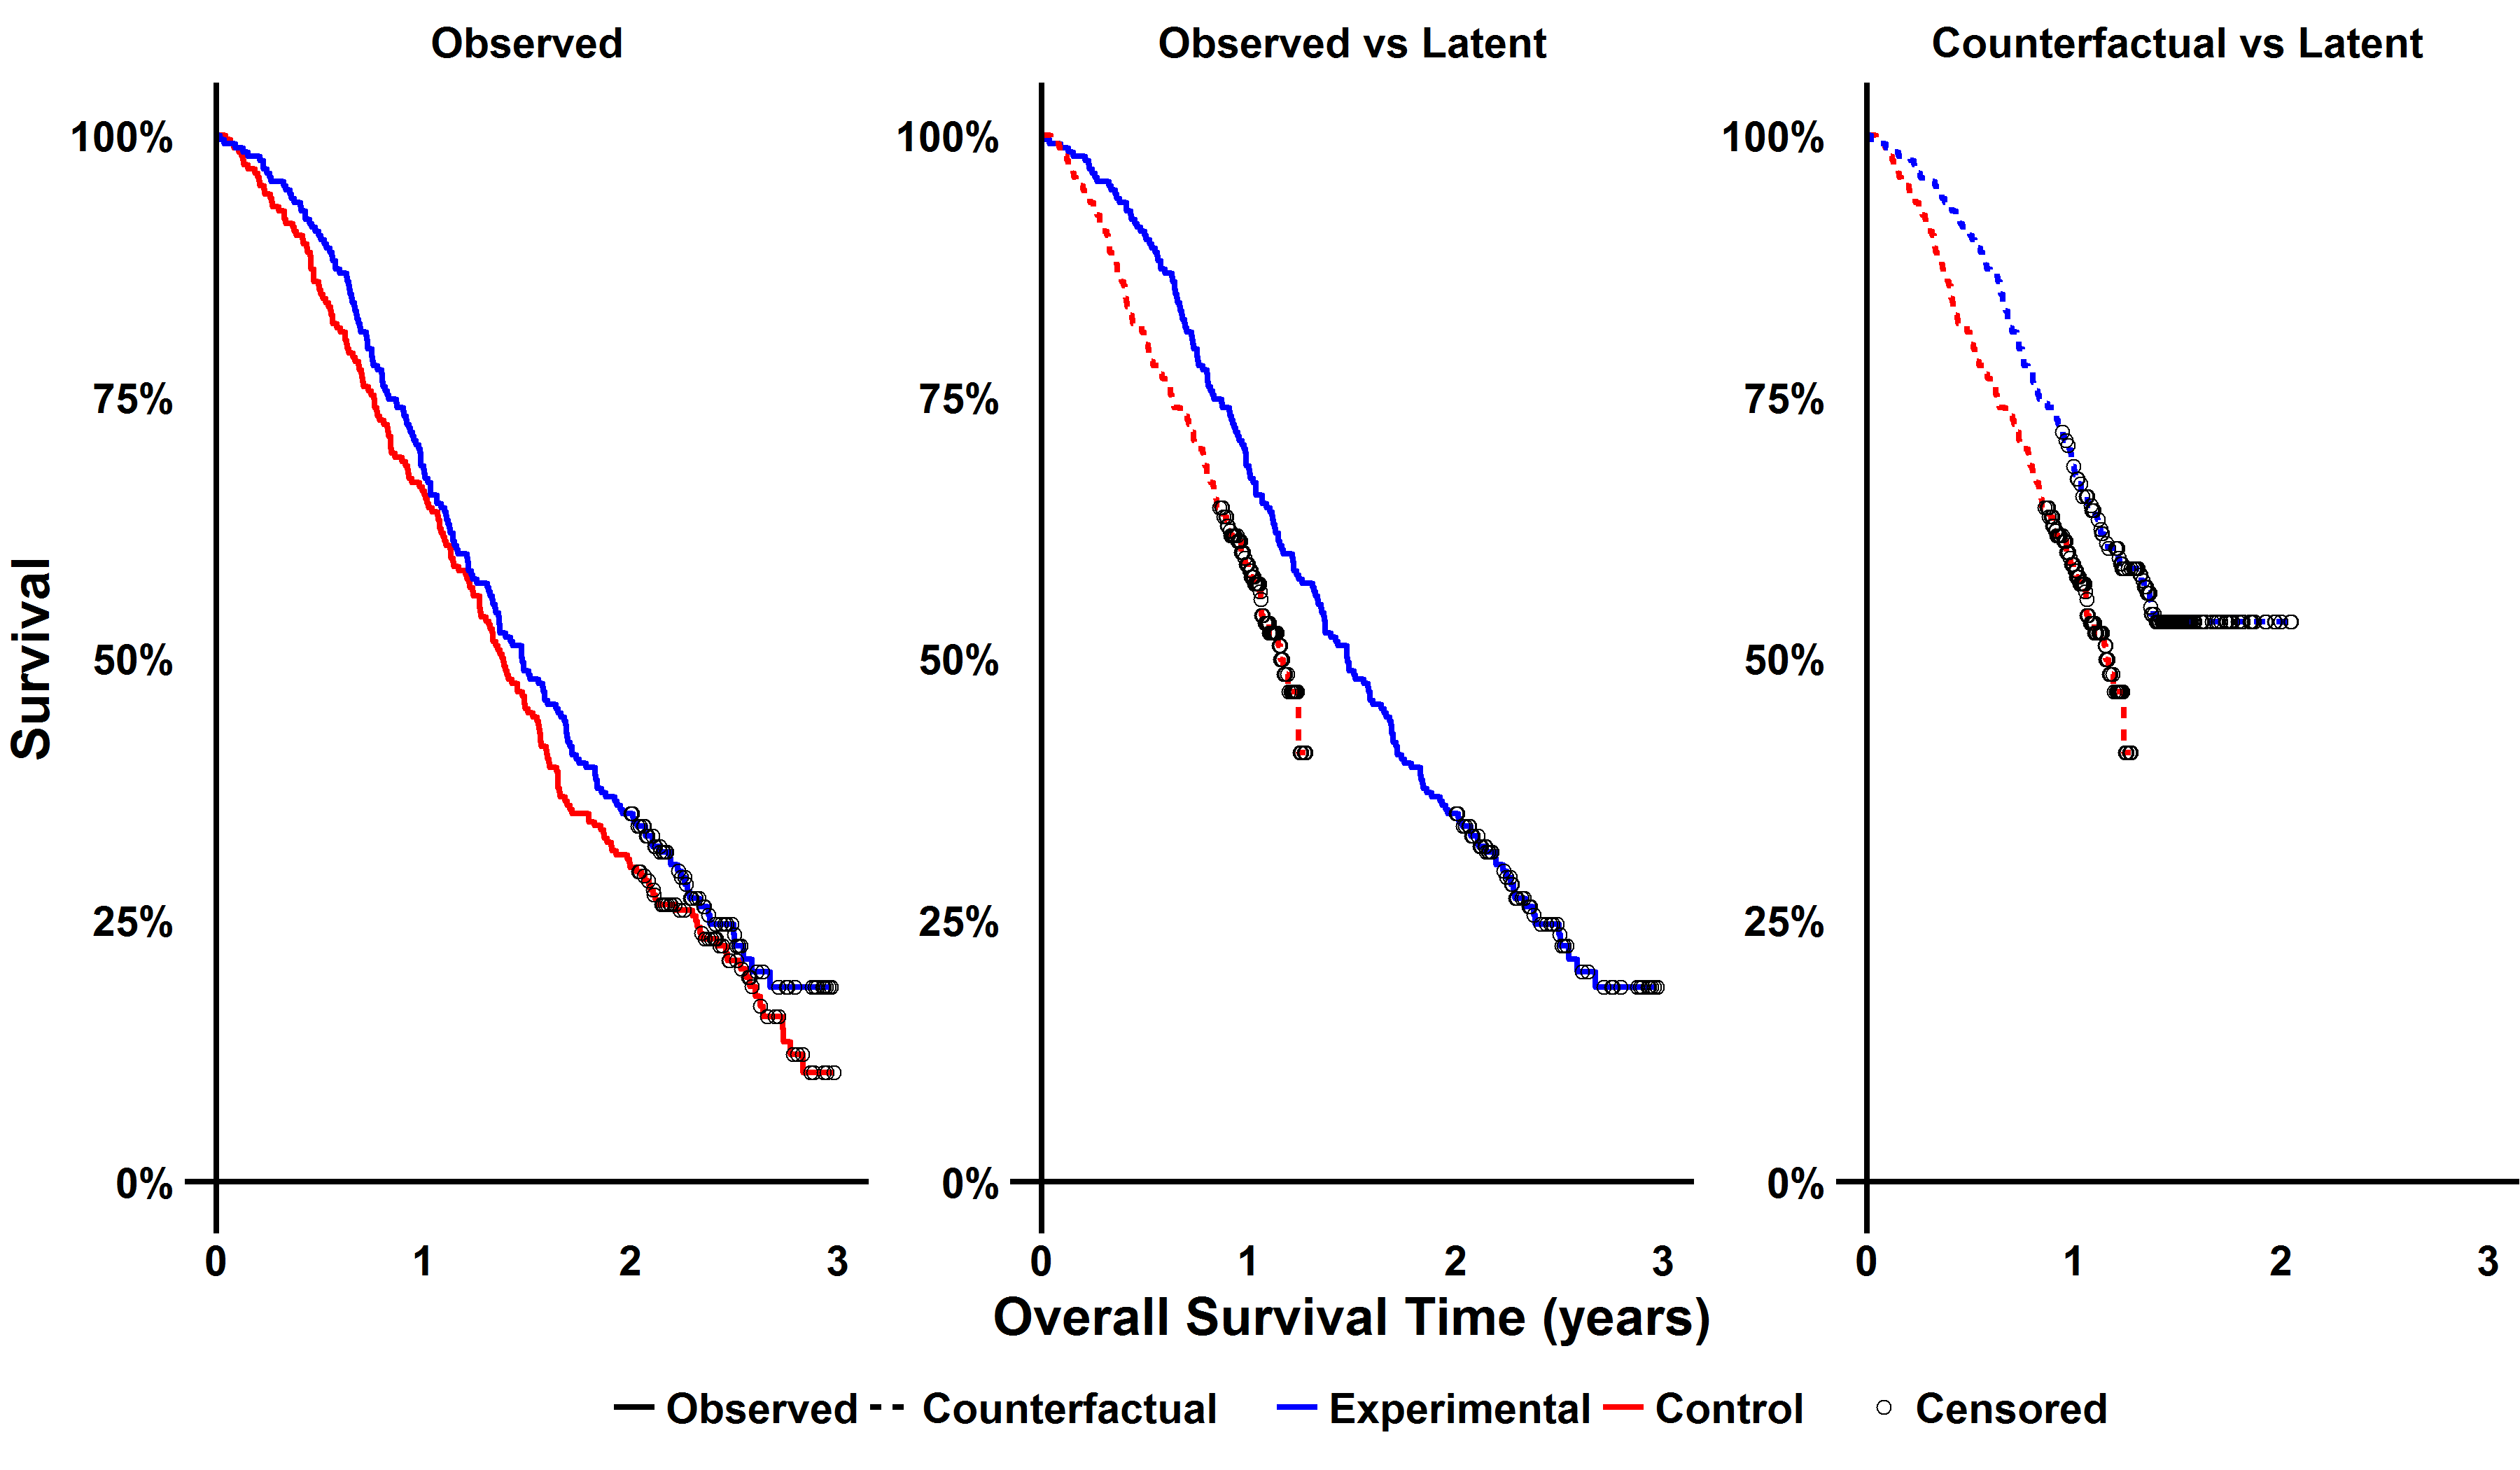
\includegraphics[width=15cm]{images/chap_methrev/example_cfact.png}
\caption{\label{F:methrev:excfact} Illustration of the different comparisons that can be made to derive corrected survival times for a simulated data set. the left panel shows the observed data $T_i$. The middle panel illustrates the comparison of $T_i$ and $U_i$ suggested by \cite{Latimer2014}. The right panel shows the comparison of $V_i$ suggested by \cite{Robins1991} where for the experimental arm the observed treatment history is applied to the latent survival time.} 
\end{figure}





Regardless of approach taken once counter-factual survival times have been estimated they can be used to estimate other counter-factual statistics such as a Hazard Ratio by fitting a Cox model. \cite{White1999} notes that while point-estimates can be taken directly from the model ``The $p$-values and standard errors from this model do not reflect the uncertainty in the accelerated life model parameter''. Indeed they suggest to either bootstrap confidence intervals or construct ``symmetrical confidence intervals for the log hazard ratio using the ITT $p$-values''. This can be done by deriving the standard error as $SE(\hat{\beta}) = \frac{\hat{\beta}}{Z(0)}$ where $\hat{\beta}$ is the log hazard ratio estimated from the counter-factual Cox model and $Z(0)=Z(\psi|\psi=0)$ is the standard normal value from the rank test used in the g-estimation process for the ITT comparison.




\section{Iterative Parameter Estimation (IPE)}


\cite{Branson2002} propose another randomization based approach which uses a similar modelling framework to the RPSFT model by relating observed survival time ($T_i$) with an unobserved latent survival time ($U_i$). This relationship is defined by the model in Equation \ref{E:BWIPE} where $A_i$ is the time a patient starts experimental therapy.
\begin{equation}
U_{i} = A_i + e^{-\eta}( T_{i} - A_i )
\label{E:BWIPE}
\end{equation}
It can be seen that this is similar to the ``treatment group'' approach to RPSFT and makes the same common treatment effect assumption. 

\subsection{Parameter estimation}
The main difference with RPSFT is the approach taken to estimate the parameter $e^{-\eta}$. To do this it is assumed that the survival times follow a parametric accelerated failure time distribution such as a weibull. The parameter is then estimated in an iterative fashion as follows:
\begin{enumerate}
\item $\exp(-\hat{\eta}_1)$ is estimated by comparing the treatment arms as randomized using a parametric AFT model.
\item $U_{i,1}$ is estimated by using the estimate $\exp(-\hat{\eta}_1)$  in Equation  \ref{E:BWIPE}. \label{step1}
\item $\exp(-\hat{\eta}_j)$  is estimated by comparing the $T_i$ for patients randomized to experimental treatment with the $U_{i,j-1}$ for patients randomized to control therapy using a parametric AFT model. 
\item The estimates $\exp(-\hat{\eta}_j)$ and $\exp(-\hat{\eta}_{j-1})$  are compared and if close enough\footnote{\cite{Branson2002} suggest a tolerance of $10^{-5}$.} the algorithm is said to have converged. If the algorithm does not converge then $U_{i,j}$ is estimated by substituting $\exp(-\hat{\eta}_j)$ into Equation \ref{E:BWIPE}. Steps 3 to 4 are then repeated until convergence is reached.
\end{enumerate}

\subsection{Handling Censored Data}
\label{S:chap_methrev:MIPE}

\cite{Branson2002} claim, that unlike RPSFT, ``IPE requires recensoring survival times only if they are projected beyond the end of the study. Consequently, the occurrence of recensoring is limited to those patients who switch treatment in the control arm, and will be required only if experimental treatment is detrimental compared with control.''

\cite{White2006} and \cite{Zhang2016} challenge this approach and argue that the same censoring rules on the latent survival ($U_i$) time scale need to be implemented as used for RPSFT. That is the estimated latent survival times for all control arm patients $U_{i,j-1}$ need to be recensored not just those of switchers. The recensoring time for a patient is dereived identically to RPSFT as $C_i^\star$ calculated with Equation \ref{E:MIPEcens} where $C_i$ is the patients known potential administrative censoring time. This implementation of IPE with corrected censoring rules is referred to by \cite{Zhang2016} as the modified IPE (MIPE).

\begin{equation}
\label{E:MIPEcens}
C_i^\star(\eta) = \min \left( C_i, C_i e^{-\eta} \right)
\end{equation}

\subsection{Estimating a corrected Hazard Ratio}

Estimation of a corrected Hazard Ratio follows the same procedure as with the RPSFT method with the choice being to take these from the parametric model directly\footnote{Assuming a Weibull is used which has both an proportional hazards and accelerated failure time interpretation.} or by doing a comparison of the $T_i$ for the experimental arm with the $U_i$ for the experimental arm. Similarly to RPSFT it is noted by \cite{Zhang2016} that care has to be taken with estimating confidence intervals.
\begin{quote}
Although it is relatively easy to calculate the point estimate [of treatment effect], the calculation of its variance (and CI) is not straightforward. It is not valid to use the variance and CI from the last iteration from the MIPE algorithm because it does not incorporate the variability of the point estimate from the previous iteration. Instead, the bootstrap method is usually recommended.
\end{quote}

\section{Two Stage Accelerated Failure Time (AFT) model }

\cite{Latimer2013} introduce a simplified observational method that requires less data than the IPCW. The approach is too assume there is a single timepoint when all patients have a choice to switch or not switch and to define a secondary baseline at this timepoint. For all control arm patients who reach this ``second baseline'' they are designated as switcher/nonswitcher and compared, adjusting for other covariates measured at the ``second baseline'' in an AFT model to get an adjusted estimate for the effect of switch treatment. As an AFT model is used, the survival time for the patients who switch can be shrunk using this estimate of treatment effect. In practice given the design of oncology trials this this method is usually applied with time of progression  taken as the ``second baseline'' though as noted in Section \ref{S:chap_intro:pattern} this pattern of switching may not always apply. 

\subsection{Estimating counterfactual survival}

Estimation of the counterfactual survival time is done by partitioning the overall survival time for control arm patients into progression free survival (PFS) and survival post progression (SPP) as shown in Figure \ref{F:chap_intro:pfsandpps}. A parametric AFT model is then fit to the SPP times adjusting for covariates captured at the time of progression as shown in Equation \ref{E:chap_meth:2saftm1} where $X_{SWITCH}$ is the indicator for switch and $X_1 \ldots X_p$ are the additional covariates to adjust for.

\begin{align}
S(t_{SPP}; \theta) &= S_0(\theta t_{SPP}) \label{E:chap_meth:2saftm1} \\
\theta &= \exp(-[\eta X_{SWITCH} + \beta_1 X_1 + \ldots + \beta_p X_p]) \nonumber
\end{align}

The counterfactual survival time ($U_i$) for a patient $i$ can then be defined as shown in Equation \ref{E:chap_meth:2saftm2} similarly to the RPSFT and IPE methods.
\begin{equation}
U_i = T_{PFS_i} + T_{SPP_i} e^{-\eta}  \label{E:chap_meth:2saftm2}
\end{equation}

It is important to note that this approach will only yield correct estimates if the model shown in Equation \ref{E:chap_meth:2saftm1} is correct and all covariates that could influence survival are collected at the time of progression.

\subsection{Handling Censored Data}
\label{S:chap_meth:2saftcens}
\cite{Latimer2016} note that as this method is defining a counterfactual survival time the same concerns around informative censoring on  the counterfactual time scale as discussed for the RPFST and MIPE methods apply. As such they advocate censoring the $U_i$ at $C_i^\star(\eta)$ defined as shown in Equation \ref{E:chap_meth:2saftcens} where as before $C_i$ is the patients known potential administrative censoring time.
\begin{equation}
\label{E:chap_meth:2saftcens}
C_i^\star(\eta) = \min \left( C_i, C_i e^{-\eta} \right)
\end{equation}
It can be seen that this is perhaps a conservative approach as it makes the assumption that each control arm patient could potentially be on switch treatment for the whole of their follow-up period which is clearly not possible. A potential alternative censoring mechanism which would require less observations to be censored is as shown in Equation \ref{E:chap_meth:2saftcens2} where $K$ is the potential minimum switching time (such as the shortest PFS time observed within the trial).
\begin{equation}
\label{E:chap_meth:2saftcens2}
C_i^\star(\eta) = \min \left( C_i, K + (C_i - K) e^{-\eta} \right)
\end{equation}

\subsection{Estimating a corrected Hazard Ratio}

Estimation of a corrected Hazard Ratio follows the same procedure as with the RPSFT and MIPE method by doing a comparison of the $T_i$ for the experimental arm with the $U_i$ for the control arm. As with the RPSFT and MIPE methods \cite{Latimer2016} note that confidence intervals need to be estimated through bootstrapping. 

\section{Summary}

In this Chapter a selection of methods that have been proposed to analyse trials where treatment switching has occurred are described. As discussed in Section \ref{S:chap_intro:simstudy} an approach to assess the performance of these methods is to test each method against simulated data where a known treatment effect exists. This will be the focus of the reminder of this dissertation. 



\chapter{Simulation Study Design and Methods}
\label{C:chap_sim_design}


To analyse the performance of the different methods described in Chapter \ref{CHAP:methods} simulations of clinical trials was performed. This chapter describes the overall framework used and the rationale for the choice of parameters kept fixed and those modified by scenario. Some aspects are inspired by choices made in the simulation study reported in \cite{Morden2011}.

\section{Simulation framework}

\label{section:studydesign}

\subsection{Entry and exit times}
Similar to \cite{Morden2011} a uniform distribution was assumed for entry to the study. However, to increase the amount of censoring observed enrolment was assumed to occur over a two year period with all patients censored at 3 years after the study start meaning all patients were followed for between 1 and 3 years.

\subsection{Underlying Survival Times}
Following \cite{Morden2011} a sample size of 500 patients per dataset was chosen with 250 allocated to control and experimental treatment. For all 500 patients the baseline Time to Progression (TTP) and Overall Survival (OS) were generated from a weibull distribution with survival function as shown in Equation \ref{E:chap_simdesign:weibull}. For Time to Progression the parameters chosen were $\gamma_{TTP}=1.5$ and $\lambda_{TTP}=2$, for overall survival the parameters were $\gamma_{OS}=1.2$ and $\lambda_{OS}=0.3$. From these two survival times a progression free survival (PFS) time is defined as the minimum of time to progression (TTP) and overall survival (OS). It can be seen in Figure \ref{F:chap_sim_design:exampleKM} that these parameters result in realistic survival curves compared to those seen in e.g.  \cite{EMILIA}.

\begin{equation}
\label{E:chap_simdesign:weibull}
S(t) = \exp(-\lambda t^\gamma)
\end{equation}

\subsubsection{Correlation between TTP and OS}
\label{S:chap_sim_design:corr}
As discussed in Section \ref{S:chap_intro:correlation} the main focus of this dissertation is to investigate the impact of correlation between TTP and OS so on a patient level these are forced to be correlated with a known correlation (denoted $\rho$). When selecting the range of $\rho$ to investigate Table \ref{T:chap_intro:corr} was consulted, however, this mostly reports the correlation between PFS (a composite of TTP and OS) with OS. As PFS is a composite of TTP and OS it shows a some correlation with OS even when TTP is and OS is uncorrelated as illustrated in Figure \ref{F:chap_sim_design:corr1}.
\begin{figure}[h!]
\centering
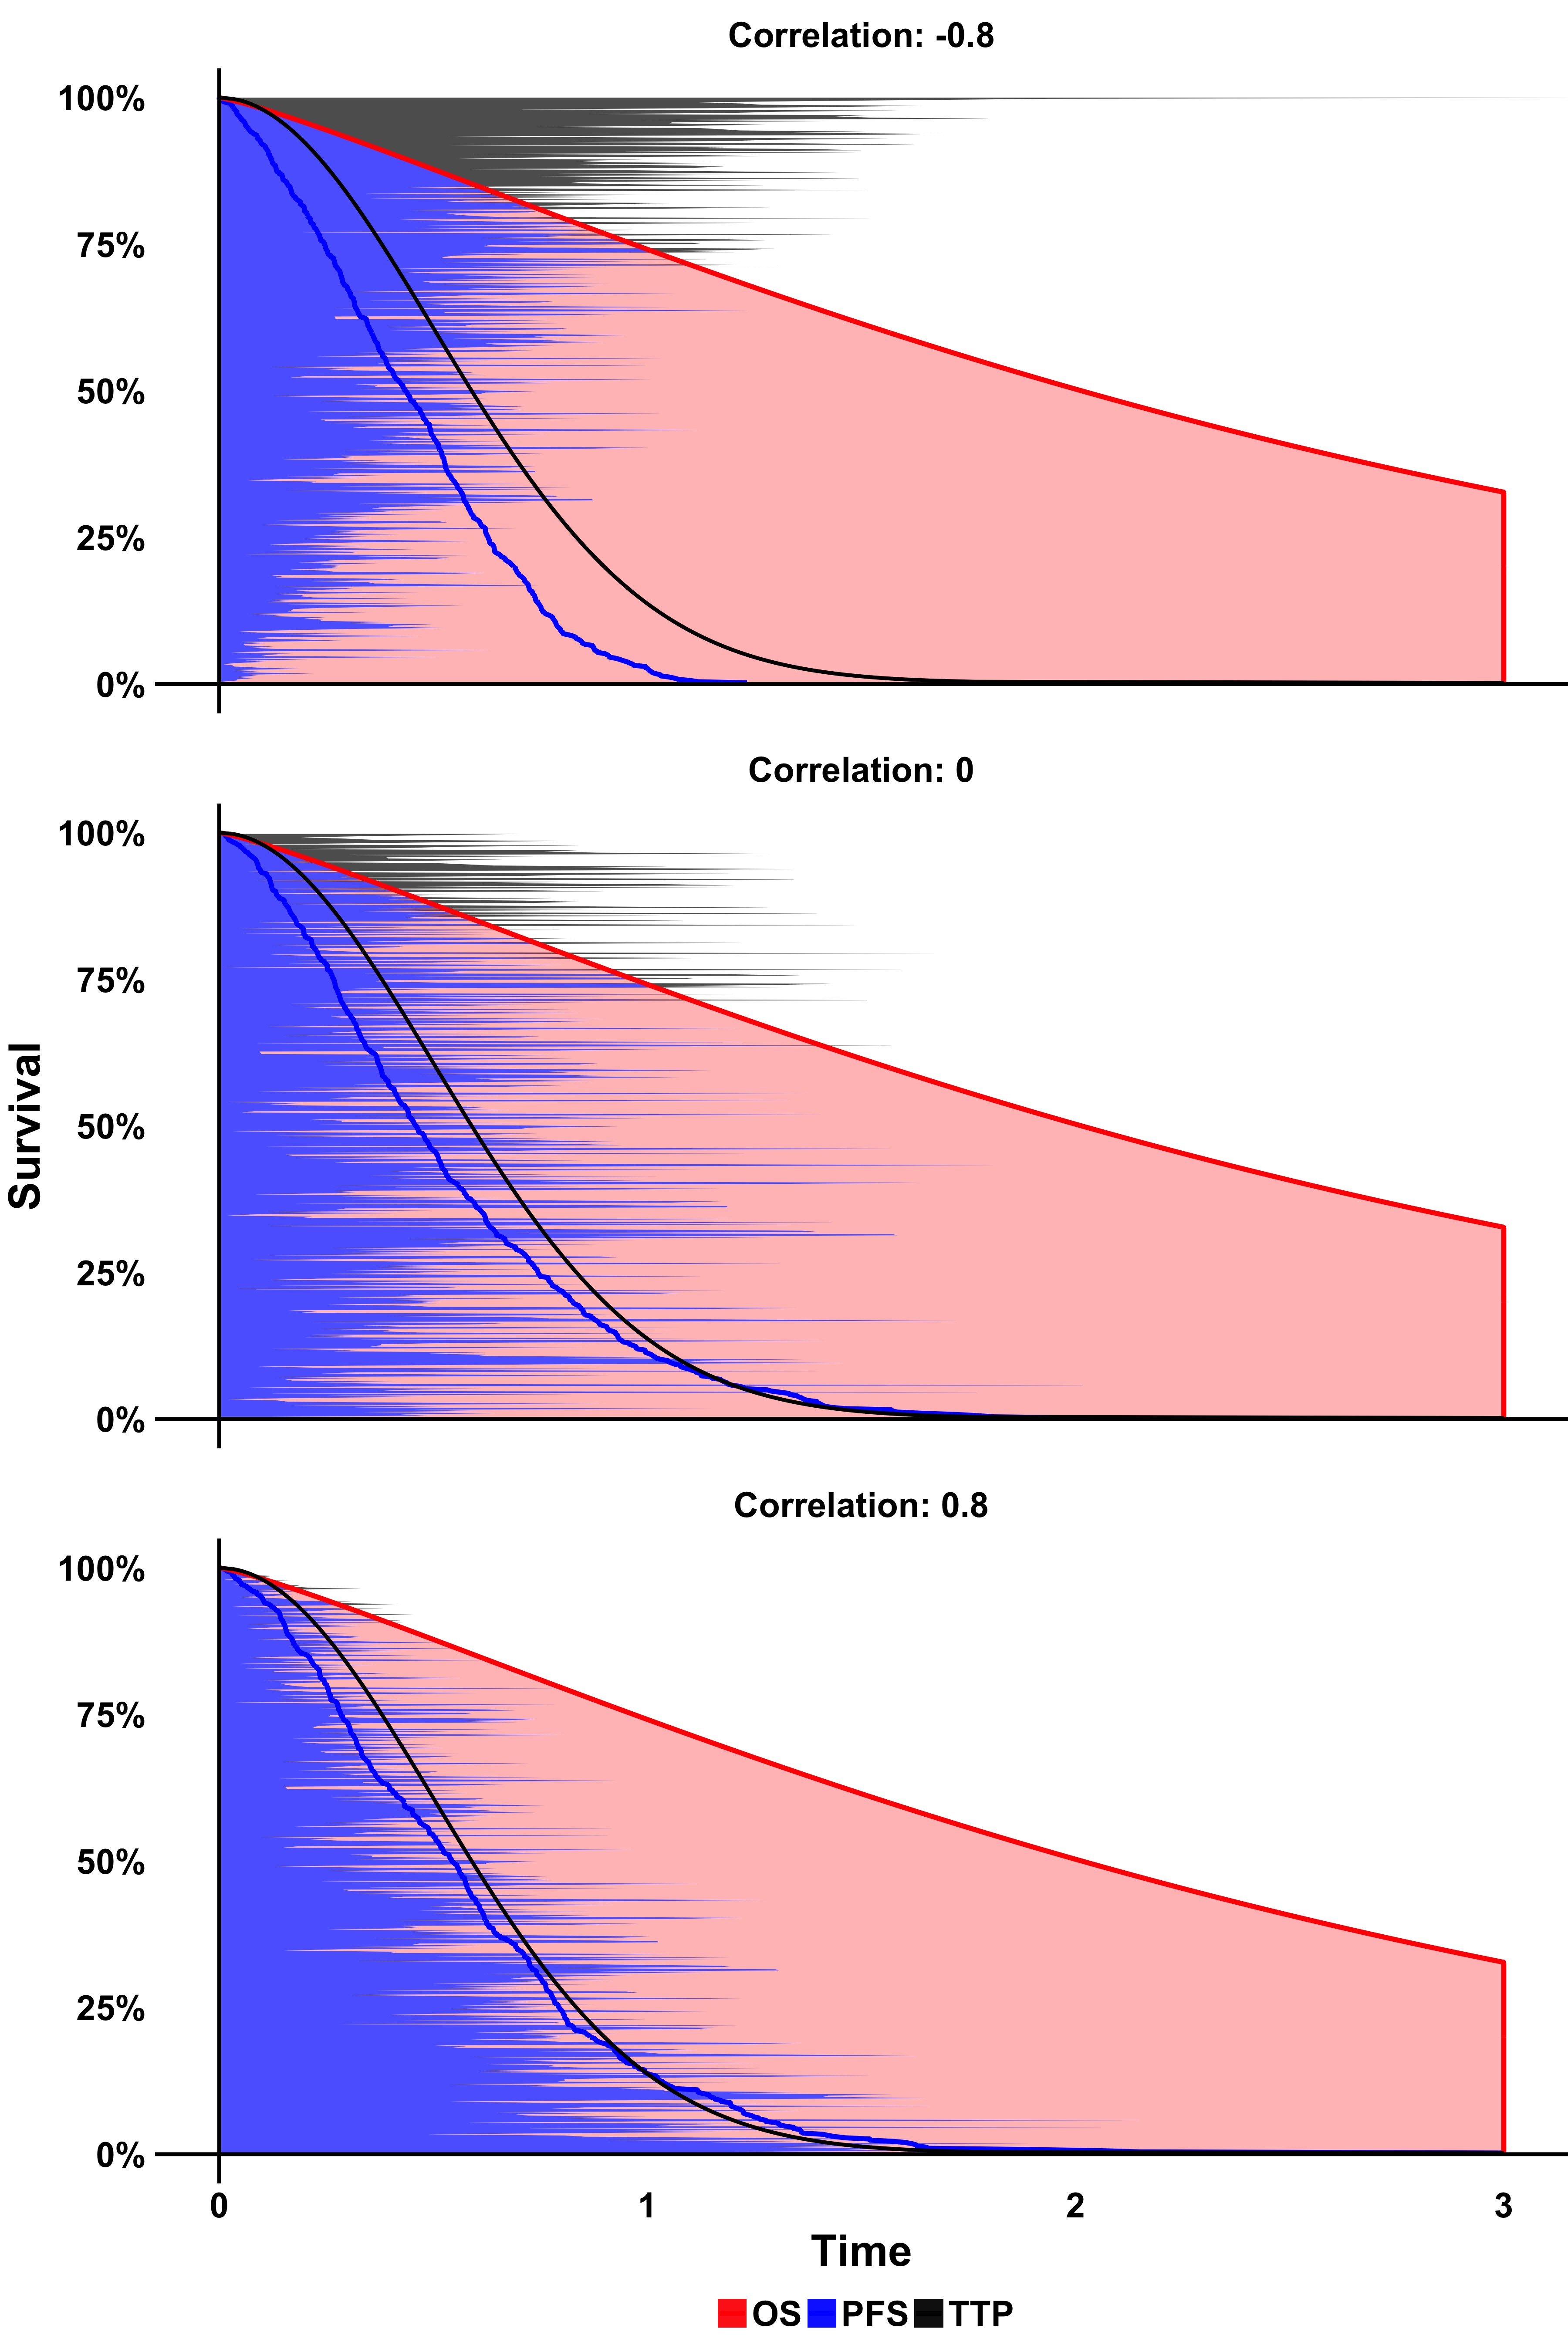
\includegraphics[width=10cm]{images/chap_simdesign/sim1corr.png}
\caption{\label{F:chap_sim_design:corr1}
An illustration of the time to progression (TTP), progression free survival (PFS) and overall survival times for strong negative, none and strong positive correlations between TTP and OS. The filled area shows the PFS and TTP by patient associated with OS. For strong negative correlation it can be seen that the TTP is often longer than OS meaning PFS is often OS in this case. For strong positive correlation it can be seen that longer TTP is associated with longer OS. With no correlation TTP is not related to OS, however, as PFS is a composite of OS and TTP it still shows some correlation with OS.} 
\end{figure}

To investigate what the resulting correlation between PFS and OS is for the simulations here the simplest method described in \cite{Buyse2007} was used. That is the correlation between the Kaplan-Meier estimates of PFS at 6 months and OS at 12 months were estimated from simulated trial data for candidate values of $\rho$ between 0 and 1 for 200 simulated trials each. The results of this are shown in Figure \ref{F:chap_sim_design:pfs_corr}. Based on this while a range of correlation between TTP and OS between 0 and 1 will be investigated a correlation of between 0.4 and 0.8 for TTP and OS seems to yield the most plausible correlations between PFS and OS.

\clearpage

\begin{figure}[h!]
\centering
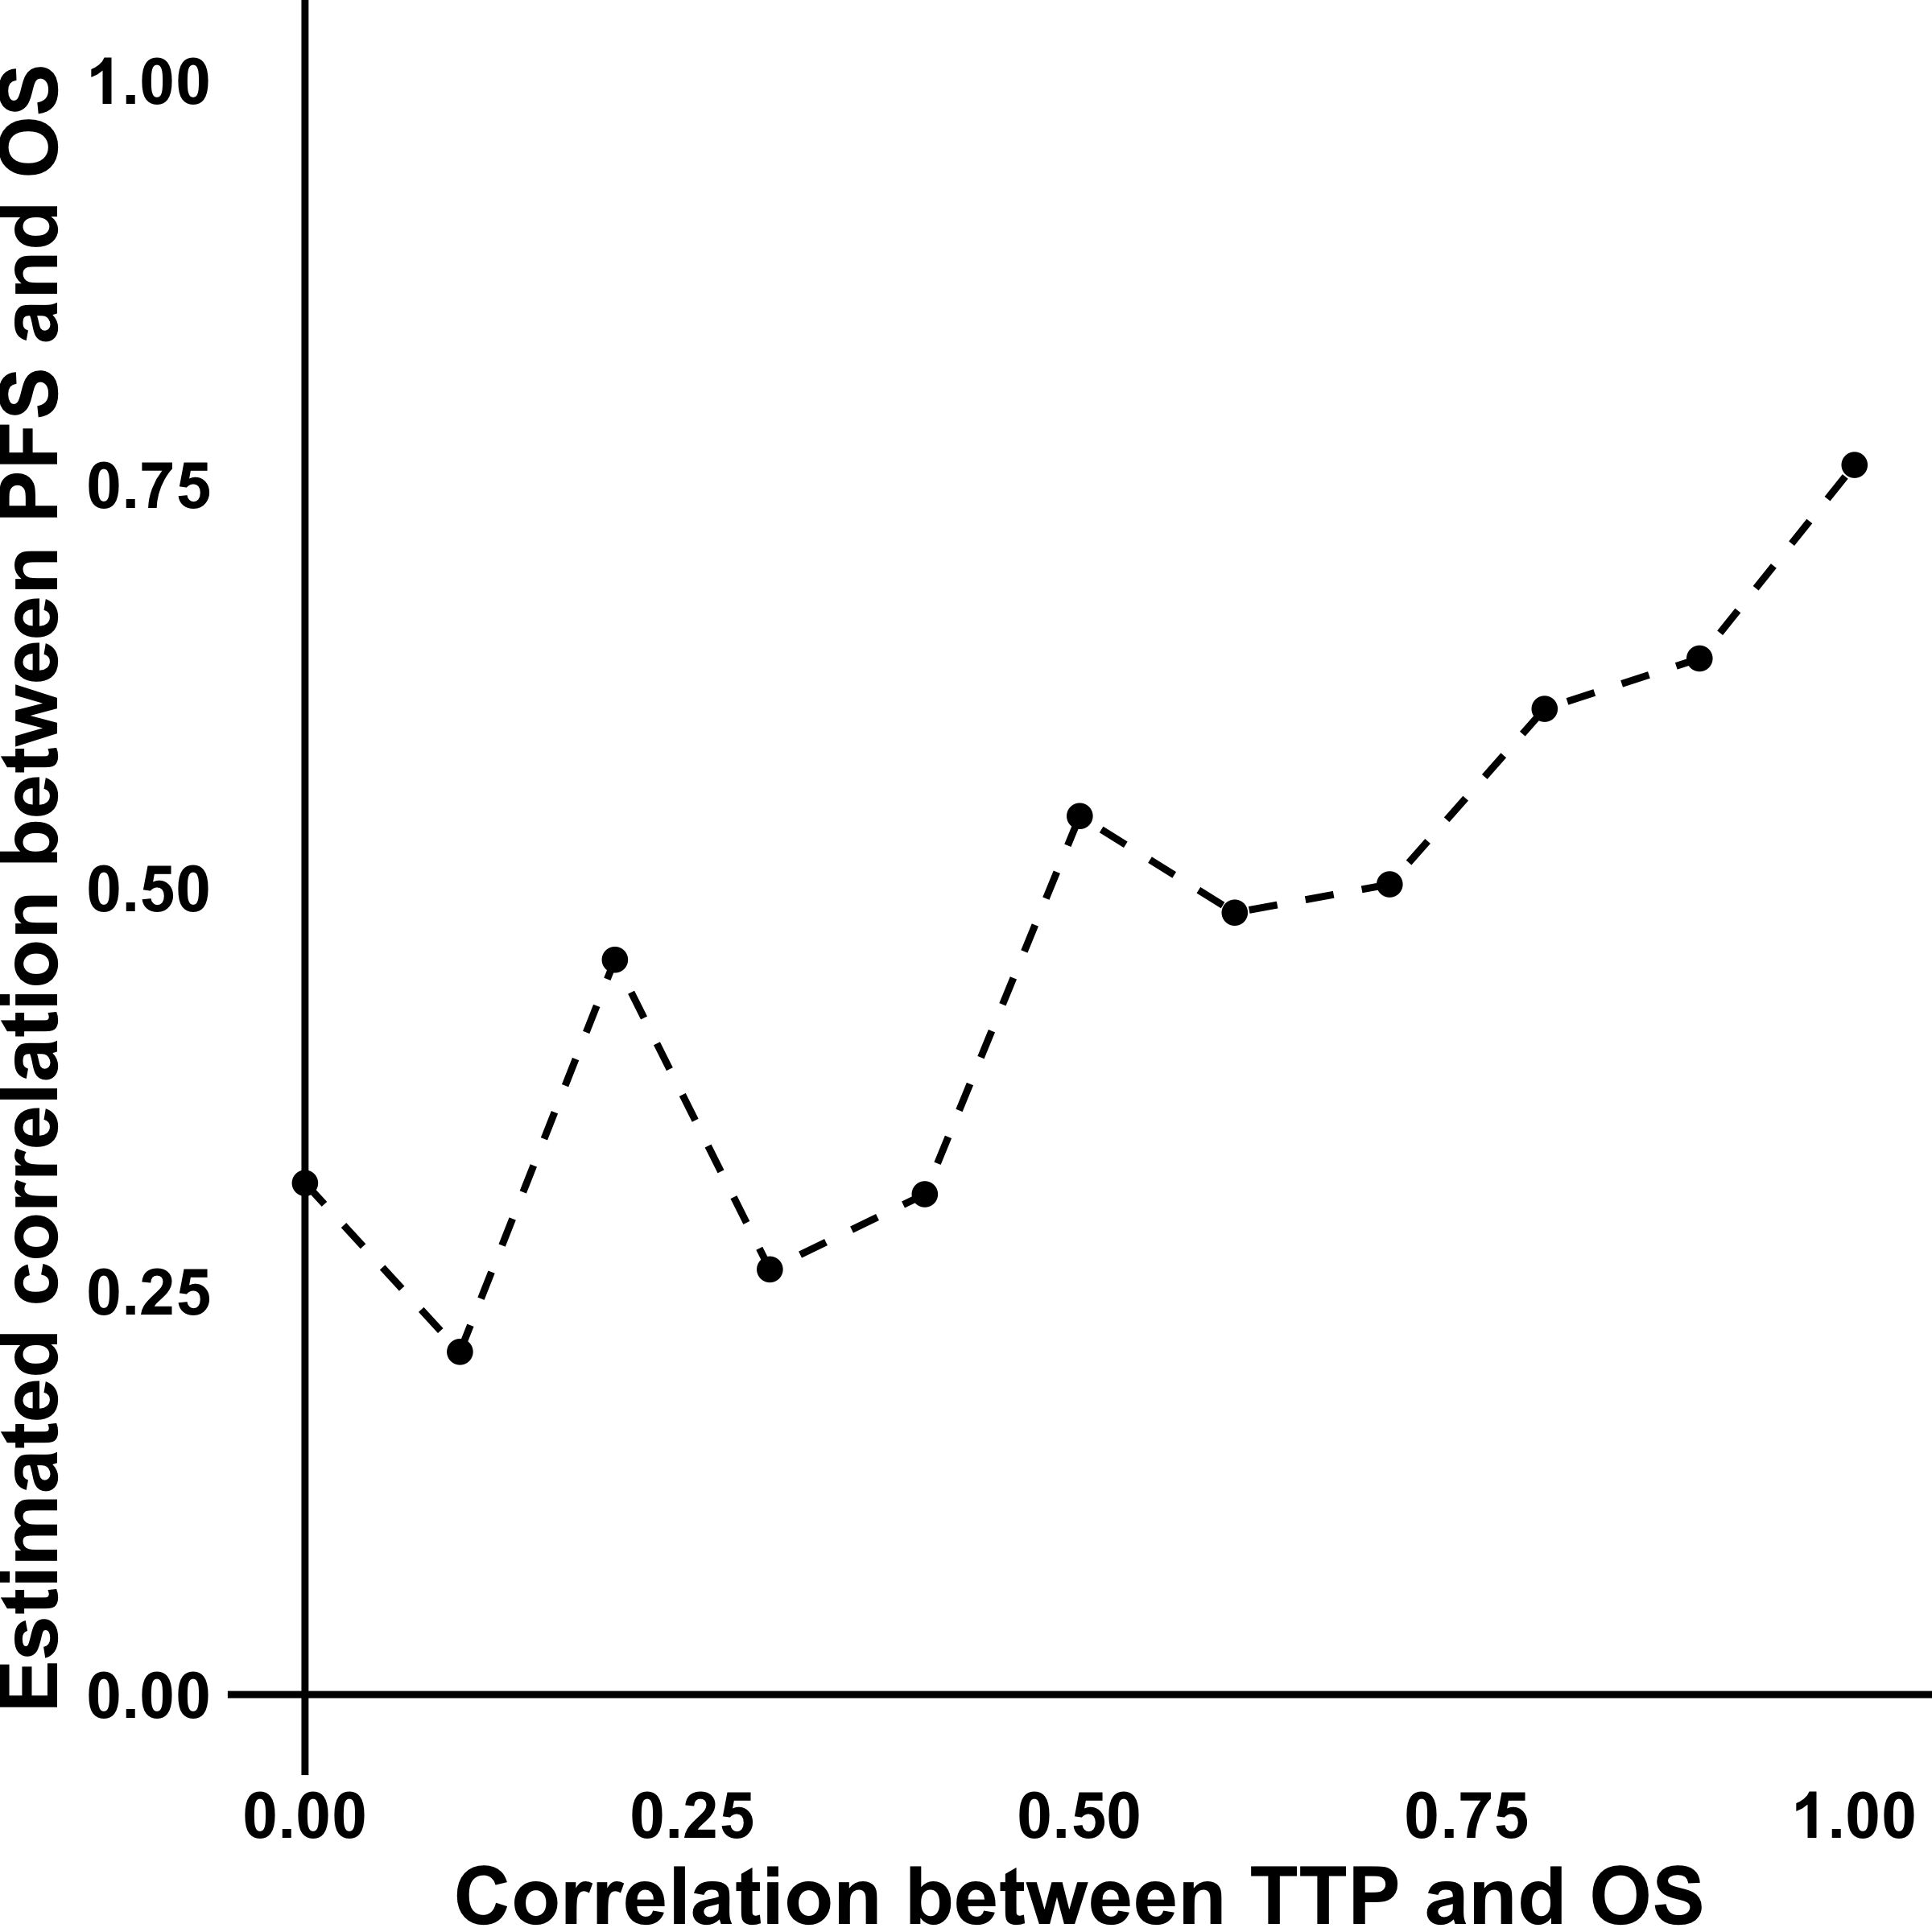
\includegraphics[width=8cm]{images/chap_simdesign/PFSOScor.png}
\caption{\label{F:chap_sim_design:pfs_corr} Estimates for the relationship between correlation in progression free survival (PFS) and OS for a range of correlations between time to progression (TTP) and overall survival (OS) using the underlying survival times.} 
\end{figure}


\subsection{Switching mechanism}
\label{S:chap_sim_design:switchmec}
As discussed in \ref{S:chap_intro:pattern} different patterns of switching may exist including restrictions on a patient and on a study level. For simplicity of simulation I am only going to consider that patients can switch at the time of progression (denoted $T_{PD}$). However, this still leaves the question of when in the study patients are allowed to switch. To control this I consider a proportion of PFS events that must occur before switching is allowed with only patients who progress after this time point being allowed to switch. When this required proportion is 0 this represents the scenario of switching being pre-planned from day 1 and otherwise it represents a scenario where switching is introduced after an interim analysis or external event.

For each simulation a target proportion of control patients who will switch to experimental therapy is defined. As only patients who progress after the defined number of PFS events occur and who have PFS less than OS and also less than follow-up time can be observed to switch this group is defined as the switch eligible population. From this switch eligible population a random selection is made so the target proportion of the control arm switches.

\subsubsection{Implications for prognosis of switch population}
Given the way survival times are generated when there is a strong positive correlation between time to progression (TTP) and overall survival (OS) the switch eligible population will contain more patients with a poor prognosis (in terms of overall survival). This is because patients with a good prognosis will have a longer time to progression and will be excluded from the switch eligible population as their progression free survival time is more likely to  extend beyond the follow up time.

\subsection{Prognostic covariates}

With all simulation studies a balance has to be made between realistically capturing the underlying problem and having a tractable problem. As discussed in the previous section introducing a correlation between TTP and OS in itself generates differential prognosis of switchers versus non-switchers given the constraints on who can be observed to switch within the study follow-up time. For this reason I choose not not to implement any additional prognostic covariates and focus instead just on the impact of correlation. 

\clearpage

\subsection{Adjusting survival times for treatment received}
\label{S:chap_sim_design:trtEffects}

For all scenarios a relatively large treatment effect on time to progression is considered. This is applied as a reduction in the hazard of progression defined as a log hazard ratio ($\beta_{pd}$) and will be constant at $\log(0.4)$ in all simulations. For all scenarios time on treatment for all patients will be fixed as time until progression i.e. it is simulated that no patients discontinue early or for any reason other than progression. For switch patients no time to second progression will be simulated but for simplicity the time on switch treatment will be taken as as the time to first progression (including the treatment effect on progression). The treatment effect on overall survival is then applied as four separate time dependent covariates representing an effect while on treatment i.e. until PD denoted $\beta_{1a}$, an effect after PD given prior treatment $\beta_{1b}$, an effect on switch treatment while on switch treatment denoted $\beta_2a$ and an effect after discontinuing switch treatment denoted $\beta_2b$. These four treatment effects are illustrated in Figure \ref{F:chap_sim_design:trtEffects}. 

\begin{figure}[h!]
\centering
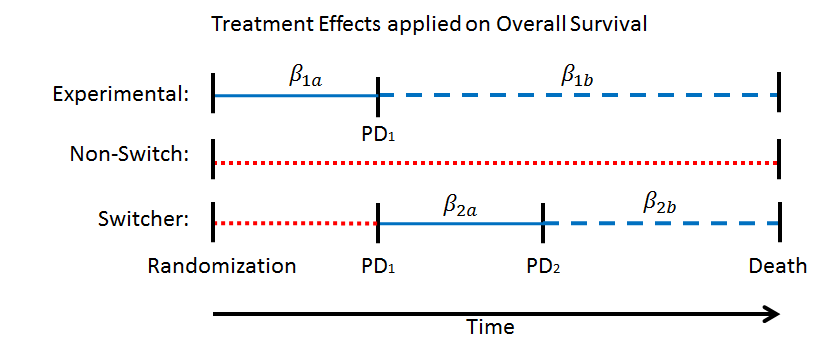
\includegraphics[width=12cm]{images/chap_simdesign/simTrtEff.png}
\caption{\label{F:chap_sim_design:trtEffects} An illustration of how the time varying treatment effects $\beta_{1a}$, $\beta_{1b}$, $\beta_{2a}$ and $\beta_{2b}$ apply to a patient randomized to the experimental arm, a non-switch patient and a switch patient. $PD_{1}$ denotes the first progression while $PD_2$ denotes the second progression after initiation of switch treatment. For simplicity only a single time to progression is simulated and assumed to apply for first and second progression.}
\end{figure}

\clearpage

\subsection{Summary of simulation parameters}

Table \ref{T:chap_sim_design:parms} shows the parameters that can be varied within this simulation framework and indicates those that are fixed across all scenarios and those which are varied across different scenarios. An illustration of the survival curves generated for two example scenarios are shown in Figure \ref{F:chap_sim_design:exampleKM}. The scenarios shown are where there is a moderate treatment effect that applies at all times ($\beta_{1a}=\beta_{1b}=\beta_{2a}=\beta_{2b}=\log(0.7)$) and a scenario where treatment reduces the risk of treatment during treatment only and has no effect afterwards ($\beta_{1a}=\beta_{2a}=\log(0.01)$ and $\beta_{1b}=\beta_{2b}=\log(1)$). 


\begin{table}[ht] 
\caption{Summary of simulation parameters}
\centering 
\begin{tabular}{ l l r}
\hline
\hline
Parameter & \multicolumn{2}{l}{Description}  \\
\hline
$\rho$    & \multicolumn{2}{l}{Correlation between TTP and OS} \\
$T_{\verb+switch+}$ & \multicolumn{2}{l}{\% patients experiencing PFS event before switch allowed}  \\
$p_{\verb+SWITCH+}$ & \multicolumn{2}{l}{Proportion of control arm who switch} \\
$\exp(\beta_{1a})$ & \multicolumn{2}{l}{Hazard ratio for OS during randomized treatment} \\  
$\exp(\beta_{1b})$ & \multicolumn{2}{l}{Hazard ratio following randomized treatment}     \\
$\exp(\beta_{2a})$ & \multicolumn{2}{l}{Hazard ratio for OS during switch treatment}     \\  
$\exp(\beta_{2b})$ & \multicolumn{2}{l}{Hazard ratio for OS following switch treatment}  \\
\hline
\multicolumn{3}{c}{Parameters held fixed across all scenarios} \\
Parameter & Description & Value  \\
\hline 
$N$ & Number of patients (with 1:1 randomization) & $500$  \\
$\exp(\beta_{pd})$ & Hazard Ratio for TTP & $0.4$  \\
$\lambda_{TTP}$ & Scale for TTP weibull baseline hazard & $2$     \\ 
$\gamma_{TTP}$  & Shape for TTP weibull baseline hazard & $1.5$  \\
$\lambda_{OS}$ & Scale for OS weibull baseline hazard  & $0.3$   \\ 
$\gamma_{TTP}$ & Shape for OS weibull baseline hazard & $1.2$   \\
\hline
\end{tabular} 
\label{T:chap_sim_design:parms}
\end{table}


\begin{figure}[h!]
\centering
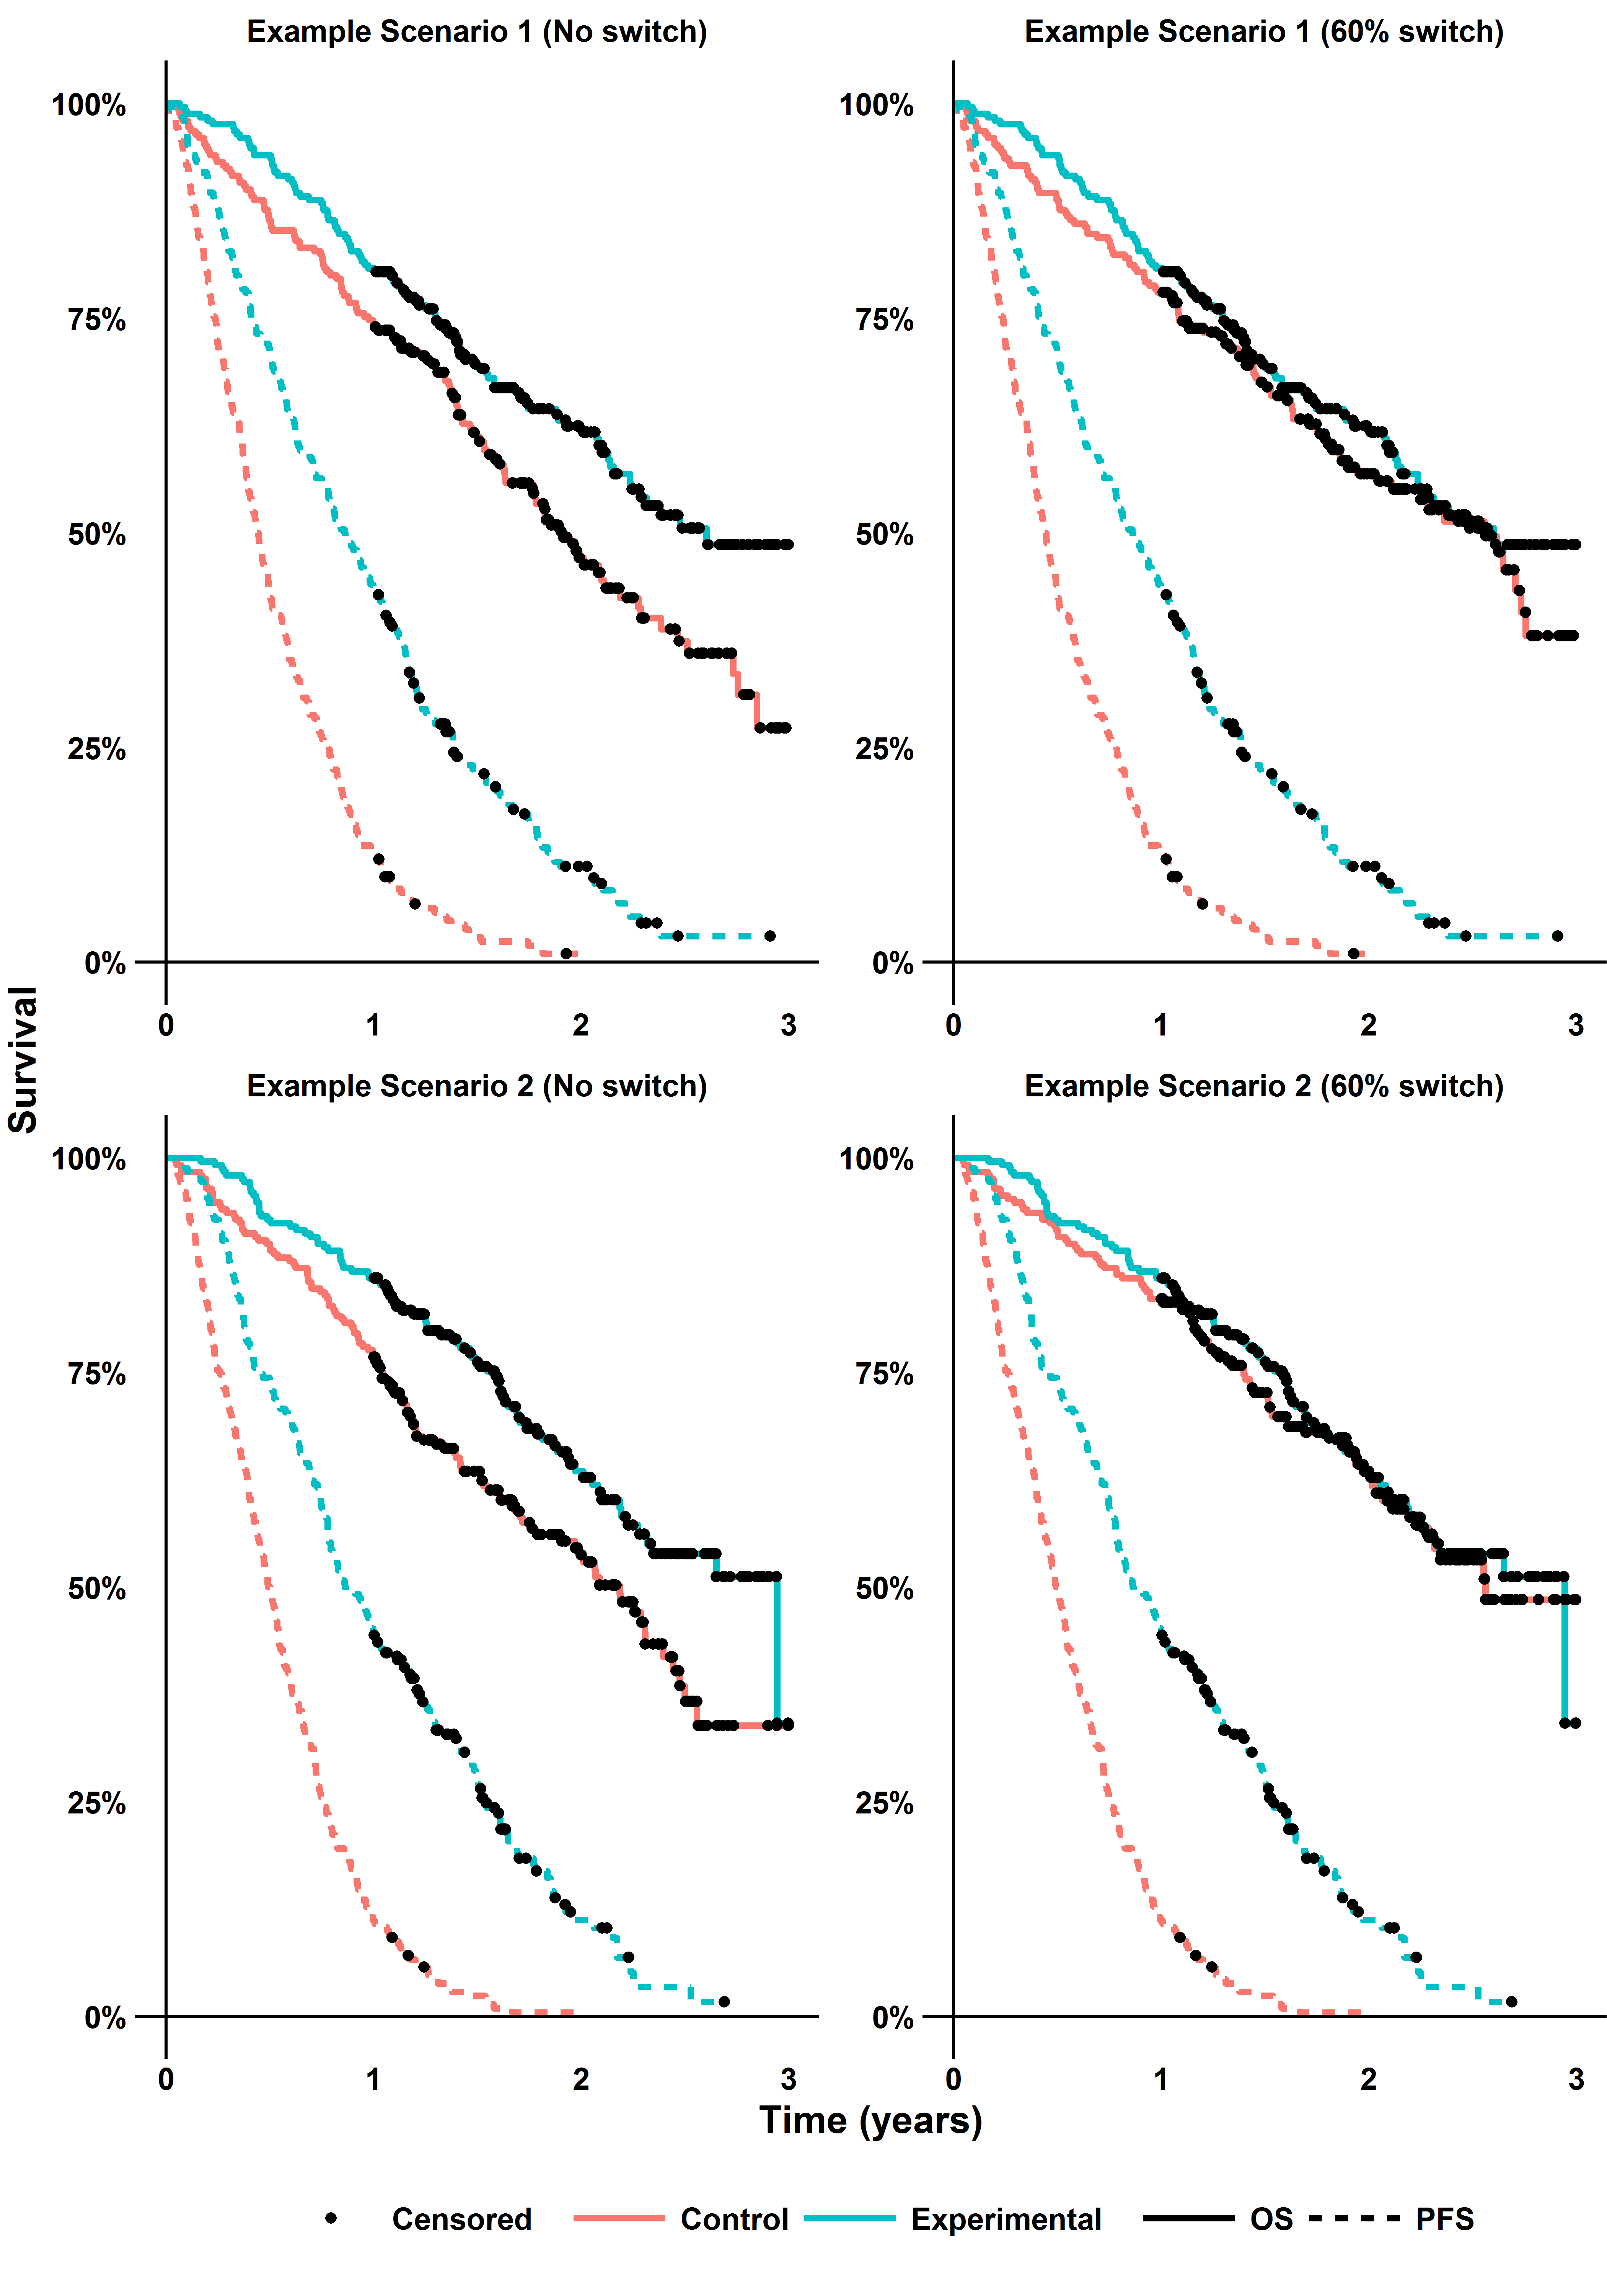
\includegraphics[width=12cm]{images/chap_simdesign/examplekm.png}
\caption{\label{F:chap_sim_design:exampleKM} The resulting survival curves for the simulation framework described in this chapter. Both example scenarios have $\rho=0.6$ and switching allowed from randomization. The treatment effects for Example Scenario 1 are $\beta_{1a} = \beta_{1b} = \beta_{2a} = \beta_{2b} = \log(0.7)$, that is a hazard ratio for experimental treatment in randomized or switch use of $0.7$. For Example Scenario 2 $\beta_{1a} = \beta_{2a} = \log(0.01)$ and $\beta_{1b}=\beta_{2a}=\log(1)$ meaning treatment only reduces the risk of death during progression free survival. While a hazard ratio of $0.01$ during treatment may seem large it is consistent with an approximate average hazard ratio for treatment of $0.65$ for a comparison of the arms as randomized.
}
\end{figure}

\clearpage


\section{Method to simulate correlated survival times incorporating treatment effect}
\label{S:chap_sim_design:simsurv}
In general if one can define the inverse of the cumulative distribution function $F^{-1}(p), p\in [0,1]$ it is possible to simulate random numbers following an arbitrary distribution through generating uniform random numbers. For survival data \cite{Bender2005} note that if the inverse of the cumulative hazard function $H(t)$ can be evaluated this can also be used as $F^{-1}(p) = H^{-1}(-log(p))$. This approach is modified to enable two correlated survival times to be generated with correlation $\rho$ as follows: 
\begin{enumerate}
\item Generate two independent standard normal random variables $X_0, X_1$ 
\item Define $X_2 = \rho X_1 + \sqrt{1-\rho^2} X_0 $ so $X_1$ and $X_2$ are correlated standard normal random variables
\item Define $U_i = \phi (X_i), i=1,2$ so $U_1$ and $U_2$ are correlated uniform random variables
\item Define $T_i = H_i^{-1}(-log(U_i)), i=1,2$ where $H_1^{-1}(t)$ and $H_2^{-1}(t)$ are inverse hazard functions so $T_1$ and $T_2$ are correlated survival times.
\end{enumerate}

Therefore to generate the correlated time to progression (TTP) and overall survival (OS) times required by this simulation framework it is just necessary to derive the inverse hazard function for TTP and OS.

\subsection{Simulating Time to Progression (TTP)}

The hazard function including a treatment effect on progression can easily be written as shown in Equation \ref{E:chap_sim_design:ttphaz} where $x_{E}$ is 1 for simulated patients randomized to experimental therapy, 0 otherwise. 

\begin{align}
\label{E:chap_sim_design:ttphaz}
h(t) &= \lambda \gamma t^{\gamma-1} x_{E} \beta_{pd} \\
\lambda &= \lambda_{TTP}, \gamma = \gamma_{TTP} \nonumber
\end{align}
\par
Survival times can then be generated for this hazard function given $u \sim U(0,1)$ following the approach of \cite{Bender2005} by using Equation \ref{E:chap_sim_design:ttpIHAZ}.
\begin{align}
\label{E:chap_sim_design:ttpIHAZ}
T_{PD} &= \left( - \frac{log(u)}{\lambda \exp( \beta_{pd} x_{E})} \right) ^\frac{1}{\gamma}
\\
\lambda &= \lambda_{TTP}, \gamma = \gamma_{TTP} \nonumber
\end{align}

\subsection{Hazard function for Overall Survival}

Based on the assumptions for treatment effect stated in the previous section it can be seen that the trial can be considered as three discrete time periods, the time from randomization to progression $T_{PD}$, the time for progression to second progression $T_{PD_2}$ and the time from second progression to death. As noted previously to simplify the generating procedure the time to first and second progression is assumed equal aside from the application of the treatment effect on progression during switch treatment, that is $T_{PD_2}$ is defined using Equation \ref{E:chap_sim_design:tpd2} based on standard properties of the weibull distribution described by \cite{collett}.
\begin{equation}
\label{E:chap_sim_design:tpd2}
T_{PD_2} = T_{PD} + \exp(\frac{-\beta_{pd}}{\gamma_{TTP}}) T_{PD}
\end{equation}
Including the time dependent treatment effects the hazard function for OS is shown in Equation \ref{E:chap_sim_design:oshaz} where $x_{E}$ is 1 for simulated patients randomized to experimental therapy, 0 otherwise; and $I(x)$ is an indicator function which is 1 if the condition $x$ is true and 0 otherwise. To simplify the notation for remainder of this section I use $\lambda, \gamma$ to represent $\lambda_{OS}$ and $\gamma_{OS}$ respectively.
\begin{align}
\label{E:chap_sim_design:oshaz}
h(t)  =  \lambda \gamma t^{\gamma-1} \{ & x_{E} \left[ I(t < T_{PD}) \beta_{1a} + I(t \geq T_{PD}) \beta_{1b} \right] \nonumber \\ 
       & (1-x_{E}) \left[ I(T_{PD} \leq t < T_{PD_2}) \beta_{2a} + I(T_{PD_2} \leq t) \beta_{2b} \right] \} 
\end{align}
\par
As this contains several time dependent covariates the derivation of an inverse cumulative hazard is more complex than seen previously and will be considered for experimental arm, non switching control arm and switch patients separately.
\subsubsection{Simulating Overall Survival (OS) for non switch control patients}
The simplest hazard function is for patients in the control arm who do not switch where this can written as  shown in Equation \ref{E:chap_sim_design:oshazcn}. 
\begin{align}
\label{E:chap_sim_design:oshazcn}
h(t) = \lambda \gamma t^{\gamma-1}  
\end{align}
As such the approach of \cite{Bender2005} can be followed to simulate times from this hazard function given $u \sim U(0,1)$  by using Equation \ref{E:chap_sim_design:osIHAZcn}.
\begin{align}
\label{E:chap_sim_design:osIHAZcn}
T_{OS} &= \left( - \frac{log(u)}{\lambda} \right) ^\frac{1}{\gamma}
\end{align}

\subsubsection{Simulating Overall Survival (OS) for experimental arm  patients}

For patients in the experimental arm the hazard function is shown in Equation \ref{E:chap_sim_design:oshaze} where $\beta_{1a}$ is the effect of experimental therapy during treatment, $\beta_{1b}$ is the effect after treatment and $T_{PD}$ is the time of progression when treatment stops. 
\begin{align}
\label{E:chap_sim_design:oshaze}
h(t) &= \lambda \gamma t^{\gamma-1} \exp\left( I( t < T_{PD} ) \beta_{1a} + I(t \geq T_{PD}) \beta_{1b} \right)  
\end{align}
By defining $\delta_1 = \beta_{1b} - \beta_{1a}$ this can be rewritten as shown as in \ref{E:chap_sim_design:oshaze2}. 
\begin{align}
\label{E:chap_sim_design:oshaze2}
h(t) &= \lambda \gamma t^{\gamma-1} \exp\left( \beta_{1a} + I(t \geq T_{PD}) \delta_1 \right) 
\end{align}

The approach of \cite{Bender2005} can not be used here, however, \cite{Austin2012} provides an extension to simulate data for a single dichotomous time varying covariate with at most one change from untreated to treated which is applicable here. Following this approach survival times can be generated using given $u \sim U(0,1)$ by using Equation \ref{E:chap_sim_design:osIHAZe}.
\begin{align}
\label{E:chap_sim_design:osIHAZe}
T_{OS} & = \begin{cases} 
 \left( \frac{-log(u)}{\lambda \exp(\beta^\prime x) } \right) ^\frac{1}{\gamma} 
 & , -log(u) < \lambda \exp(\beta^\prime x) t_0^{\gamma} \\ 
 \left( \frac{-log(u) - \lambda \exp(\beta^\prime x) t_0^{\gamma} + \lambda \exp(\beta_t) \exp(\beta^\prime x) t_0^{\gamma} }{\lambda  \exp(\beta_t)\exp(\beta^\prime x) } \right) ^\frac{1}{\gamma} 
 &  , -log(u) \geq \lambda \exp(\beta^\prime) t_0^{\gamma}
\end{cases} \\
t_0 &= T_{PD}  \nonumber \\
\beta^\prime x &= \beta_{1a} \nonumber \\
\beta_t &= \delta_1 = \beta_{1b} - \beta_{1a} \nonumber
\end{align}

\subsubsection{Simulating Overall Survival (OS) for control arm patients who switch}
For patients who switch in the control arm the hazard function can be written including two time dependent covariates as shown in Equation \ref{E:chap_sim_design:oshazcs}.

\begin{equation}
\label{E:chap_sim_design:oshazcs}
h(t)  = \lambda \gamma t^{\gamma-1} \{ I(T_{PD} \leq t < T_{PD_2}) \beta_{2a} + I(T_{PD_2} \leq t) \beta_{2b} \}
\end{equation}
By defining $\delta_2 = \beta_{2b}-\beta_{2a}$ the hazard function can be written such that both time dependent covariates only have one change each from untreated to treated as shown in Equation \ref{E:chap_sim_design:oshazcs2}.
\begin{equation}
\label{E:chap_sim_design:oshazcs2}
h(t)  = \lambda \gamma t^{\gamma-1} \{ I(T_{PD} \leq t) \beta_{2a} + I(T_{PD_2} \leq t) \delta_2 \}
\end{equation}
 This is not a scenario covered by \cite{Austin2012}, however, the derivations to create a suitable inverse hazard function are shown in Appendix \ref{A:genweib}. Using this derivation Equation \ref{E:chap_sim_design:osIHAZcs} can be used to generate suitable survival times given $u \sim U(0,1)$.
\begin{align}
\label{E:chap_sim_design:osIHAZcs}
T_{OS} & = \begin{cases} 
 \left( \frac{-\log(u)}{\lambda } \right)^{\frac{1}{ \gamma}}
 & , -\log(u) < \lambda  t_1^\gamma\\ 
  \left( \frac{-\log(u) - \lambda t_1^{\gamma} + \lambda \exp(\beta_{t1}) t_1^{\gamma} }{\lambda \exp(\beta_{t1})} \right) ^\frac{1}{\gamma} 
 &  ,\lambda  t_1^\gamma \leq -\log(u) < k \\
  \left( \frac{-\log(u) - \lambda t_{1}^{\gamma} - \lambda \exp(\beta_{t1}) ( t_{2}^{\gamma} - t_{1}^{\gamma}) +  \lambda \exp(\beta_{t1}+\beta_{t2}) t_{2}^{\gamma} } 
 {\lambda \exp( \beta_{t1}+\beta_{t2})}  \right)^{\frac{1}{\gamma}} 
 &  , k \leq -\log(u) 
\end{cases} \nonumber \\
 k &=  \lambda  t_1^\gamma + \lambda \exp(\beta_{t1})(t_2^\gamma - t_1^\gamma) \\
 t_1 & =  T_{PD}\nonumber \\
 \beta_{t1} &= \beta_{2a} \nonumber \\
 t_2 & =  T_{PD_2} \nonumber \\ 
 \beta_{t2} &= \delta_2 =  \beta_{2b}-\beta_{2a} \nonumber 
\end{align}

\section{Summary}

Having outlined a moderately flexible simulation framework to generate datasets I will use this to investigate the methods described in Chapter \ref{CHAP:methods} across two simulation studies. These simulation studies use this framework to assess different patterns of treatment effects for randomized and switch treatment. The R code \citep{Rsoftware} used to generate these datasets can be found in the Appendix Section \ref{S:app_R:simgen}.

While the simulation framework described here allows switching to be allowed only after an interim analysis this will not be investigated further. This is because an initial pilot study showed that this constraint interacts with the proportion of patients who actually switch therefore confusing the interpretation. This is shown in Figure \ref{F:chap_sim_design:pswitch} where it can be seen that defining an interim after 50\% of patients had switched means the target of 60\% of patients switching could never be reached.

\begin{figure}[ht]
\centering
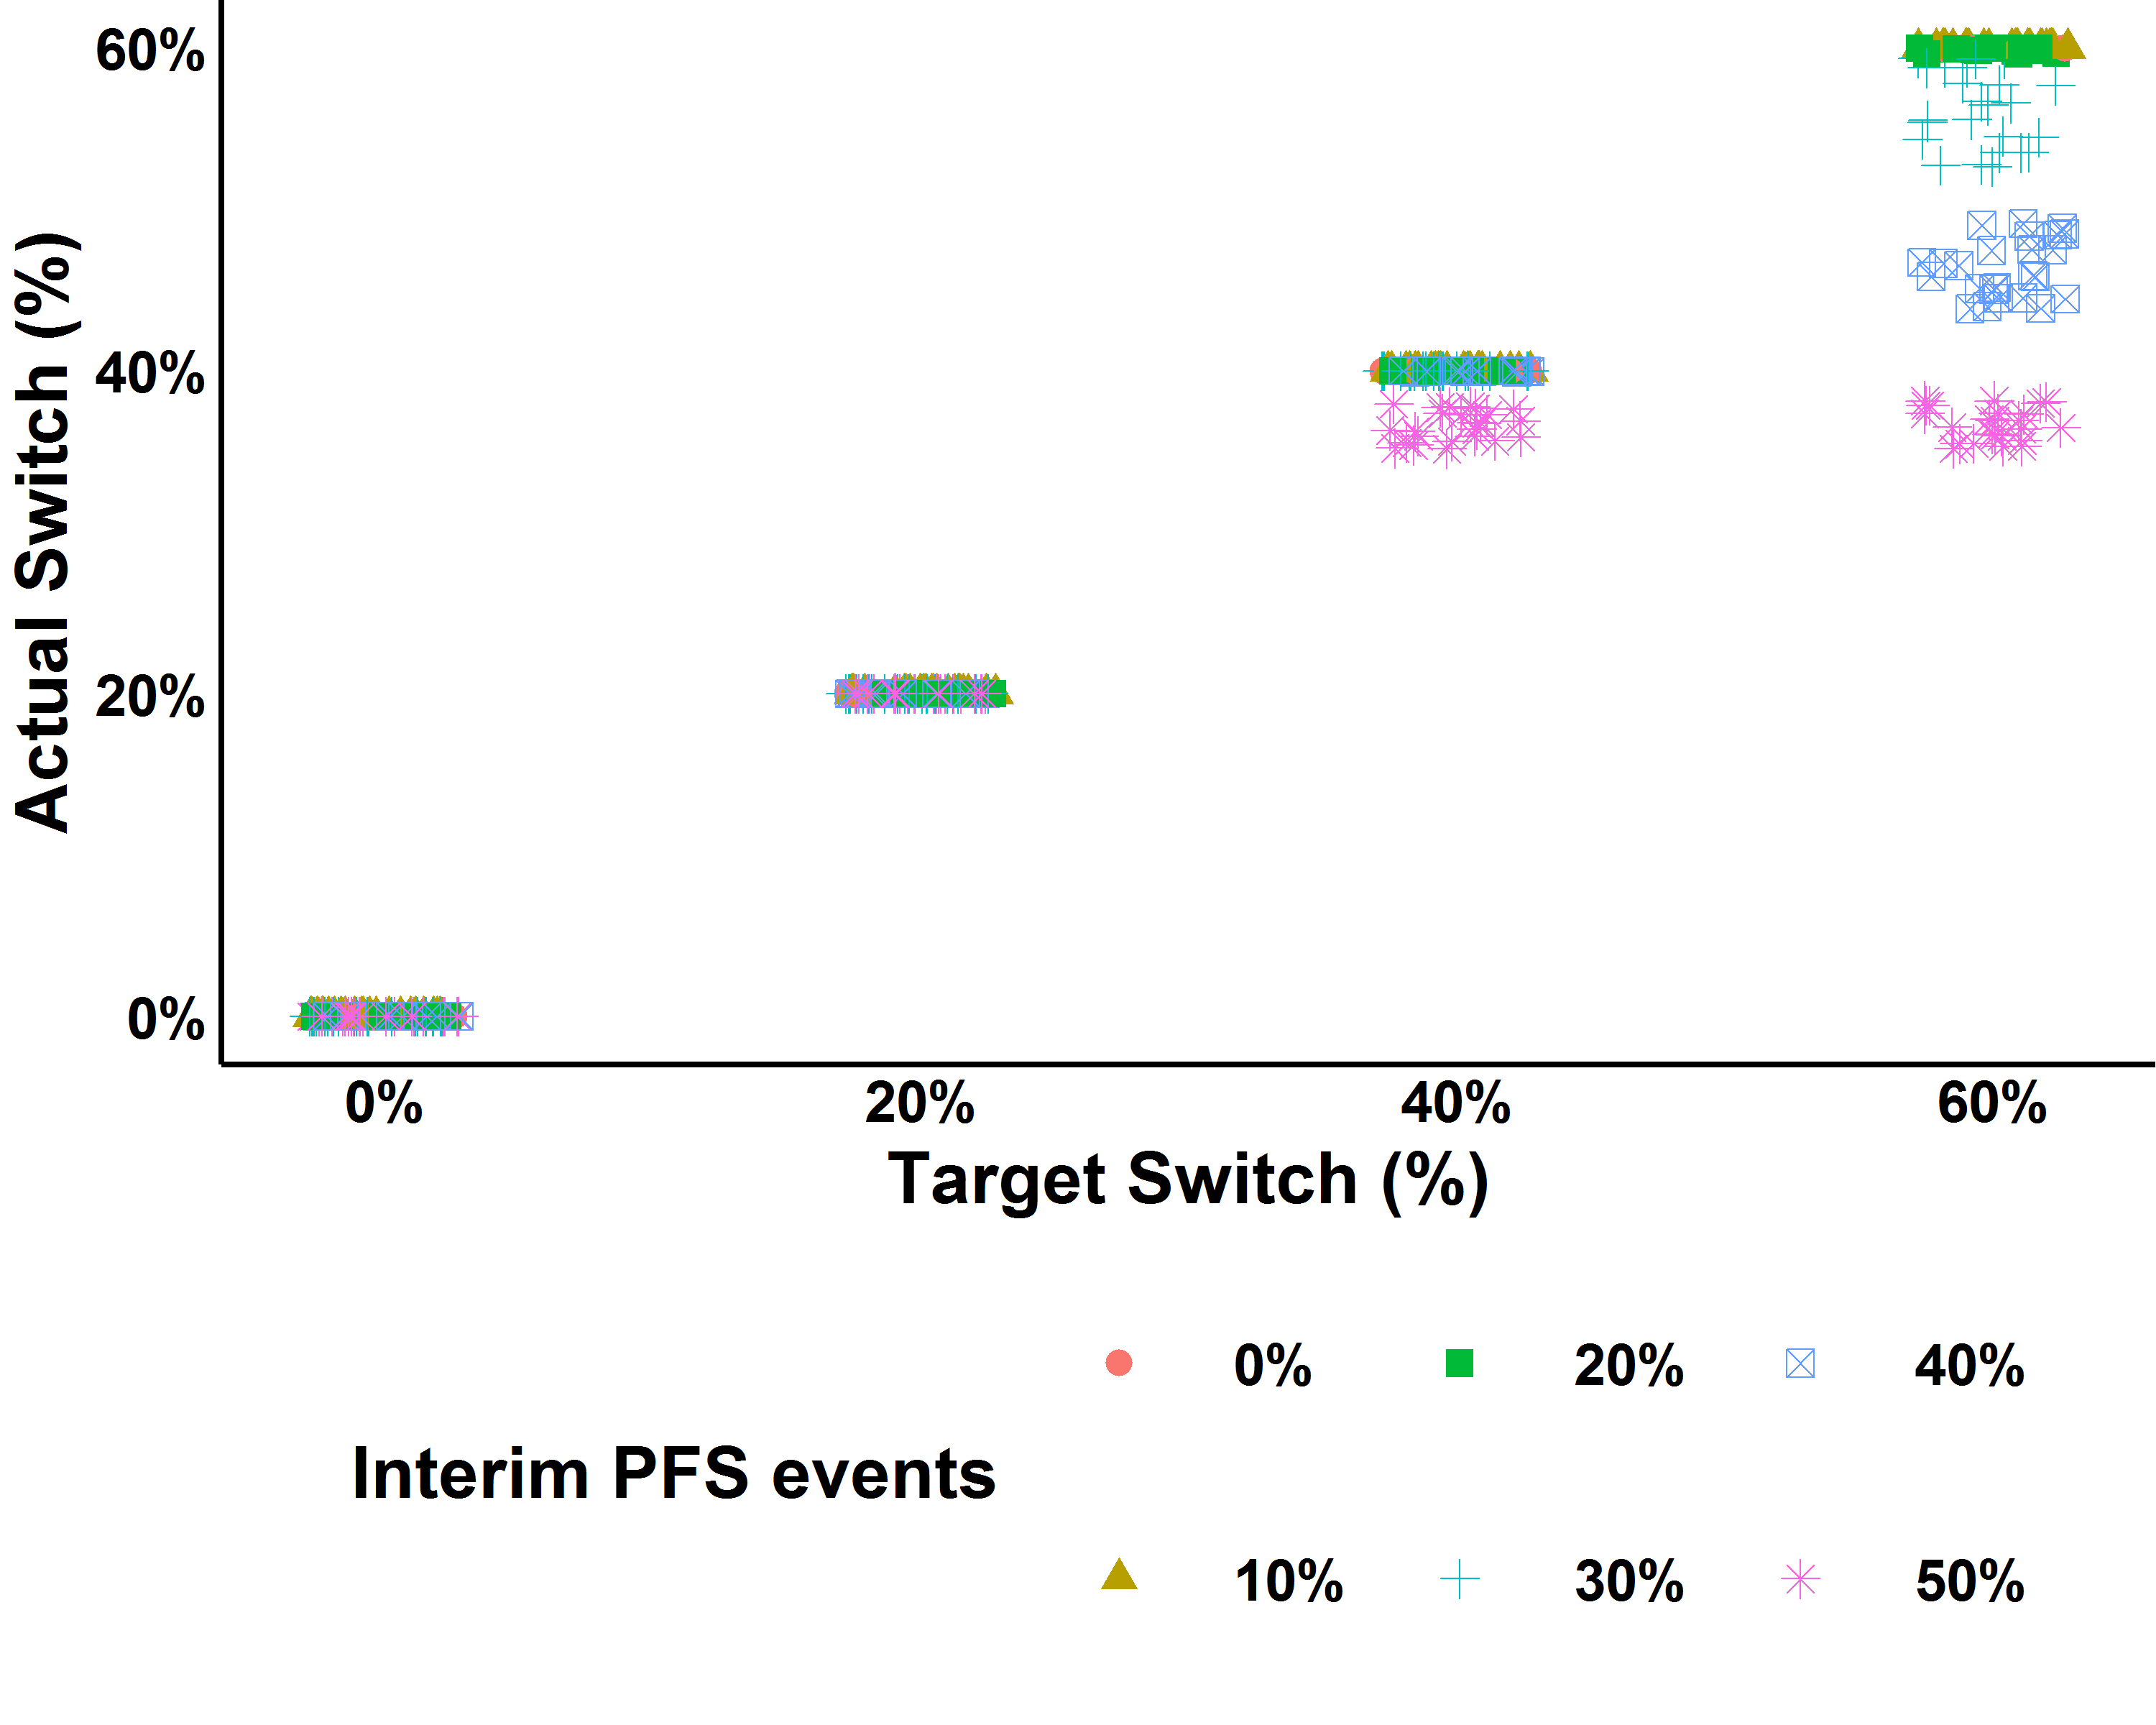
\includegraphics[width=10cm]{images/chap_simdesign/p_switch.png}
\caption{\label{F:chap_sim_design:pswitch} Figure illustrating the relationship between the percent of progression free survival events required at the interim analysis where switch is allowed and the resulting amount of switching relative to the target amount. It can be seen that by delaying switch until after an interim occurs the actual proportion of control arm patients who switch can be considerably reduced. Due to this interaction for the simulation studies described in Chapter \ref{C:chap_sim2} and Chapter \ref{C:chap_sim3} only the proportion of patients who switch will be varied. That is the interim PFS events prior to switch will be always set at 0\%.}
\end{figure}







\chapter{Simulation Study 1}
\label{C:chap_sim2}


This Simulation study is based strongly on \cite{Morden2011} with the major innovation being to induce a correlation between time to progression (TTP) and overall survival (OS) when generating the survival times.  In this simulation study I have two major objectives. Objective 1 is to confirm the results of \cite{Morden2011} once the correlations between endpoints discussed in Section \ref{S:chap_intro:correlation} are introduced. Objective 2 is to investigate the sensitivity of the rank preserving structural failure time method to variations in implementation. 

\section{Scenarios Assessed}



\subsection{Summary of Simulation Parameters}

Table \ref{T:chap_sim2:sim1parm} shows a summary of the scenarios investigated and chosen parameters. For each of the 9 basis scenarios investigated $\rho$, the correlation between Time to Progression and Overall Survival, is varied across 6 levels leading to 54 scenarios in total. For each of these 54 scenarios 1000 datasets are simulated. For this simulation the reduction in hazard due to treatment is considered to be the same during and after experimental treatment with switch patients receiving the same effect as randomized patients.

\begin{table}[ht] 
\caption{Summary of parameters for simulation study 1}
\centering 
\begin{tabular}{ l l l }
\hline
\hline
Parameter & Description & Values \\
\hline
$\exp(\beta_{1a})$        & Treatment Effect on overall survival & $0.7$, $0.9$, $1.0$ \\
                          & with $\beta_{1b}=\beta_{2a}=\beta_{2b}$    &                     \\
\hline                          
$p_{\verb+SWITCH+}$ & Proportion of control arm who switch &  $0.2$, $0.4$, $0.6$ \\
\hline
$\rho$                    & Correlation between TTP and OS  &  $0$, $0.2$, $0.4$, $0.6$, $0.8$ \\
\hline 
\end{tabular} 
\label{T:chap_sim2:sim1parm}
\end{table}


\section{Methods assessed}
\label{S:chap_sim2:methass}
Of the adjustment methods described in Chapter \ref{CHAP:methods} only a selection are assessed here. 
\subsection{Simple methods}
To estimate a Hazard ratio using simple methods the following approaches are taken.
\begin{itemize}
\item Intention-to-treat (ITT) - A Cox model will be fit to the observed data with no adjustment for treatment switching. 
\item Per-protocol Excluding Switch Patients (PP-EX) - A Cox model will be fit to the observed data excluding patients who switch.
\item Per-protocol Censoring at Switch (PP-CENS) - A Cox model will be fit to the observed data censoring patients who switch at the time of their switch.
\item Treatment as a time-varying covariate (TVC) - A Cox model will be fit to the observed data including a covariate for experimental therapy that is time dependent.
\item Switch Treatment as a time-varying covariate (TVC2) - A Cox model will be fit to the observed data including
a covariate for randomized treatment and a second covariate for switch therapy that is time dependent.
\end{itemize}
\subsection{Complex Methods}
\subsubsection{modified Iterative Parameter Estimation (MIPE)}
The IPE method including the modified re-censoring algorithm of \cite{Zhang2016} will be used as discussed in Section \ref{S:chap_methrev:MIPE}. Two approaches will be used to derive a Hazard Ratio the first will be to do a comparison of Observed ($T_i$) for experimental and Latent ($U_i$) for control survival times labelled as MIPE. The second will be to use the dual accelerated failure time and proportional hazards nature of the Weibull distribution to apply Equation \ref{E:chap_sim2:mipehr} where $\eta$ is the treatment effect estimated by Weibull regression and $\gamma$ is the shape parameter of this regression at convergence of the procedure (MIPE-WEIB). 

\begin{equation}
\label{E:chap_sim2:mipehr}
\beta = -\eta\gamma
\end{equation}

\subsection{Two-stage AFT}
To apply the two-stage AFT method it is necessary to define a secondary baseline. In this simulation the only switching that occurs is at time of progression so this is the natural choice. It is also necessary to consider any covariates that could affect survival separately to treatment at this second baseline. In this simulation no such covariates exist, however, as time to progression is correlated with overall survival this could potentially lead to situations where time to progression is predictive of the length of survival post progression. As such two AFT models will be investigated in the application of this method. In the first model the time to progression is included as a covariate (2SAFT) while for the second model is the null model where no covariates are included (2SAFT-NULL). As discussed in Section \ref{S:chap_meth:2saftcens} the recensoring algorithm described by \cite{Latimer2016} may censor more events than needed so additionally both these models will be implemented without re-censoring (labelled as NC in the results).

\subsubsection{Rank preserving-structural failure time (RPSFT) models} 
Six variations of RPSFT will be assessed in this simulation study. The first variation is the choice of test used in the g-estimation as discussed in Section \ref{S:chap_methrev:RPSFTfit} where I will investigate the use of both log-rank test and wilcoxon test. The second variation involves the choice of the ``treatment group'' or ``on treatment'' model as discussed in Section \ref{S:chap_methrev:RPSFTonep} where time on treatment will be taken to be the duration of progression free survival. The final variation was to investigate whether re-censoring of the experimental therapy arm prior to calculation of a counter-factual Hazard Ratio has in impact on the results as discussed in Section \ref{S:chap_methrev:RPSFTestHR}. The combination of these variations is detailed in Table \ref{T:chap_sim2:Sim1RPSFTlab} alongside the Label used to identify these approaches in the results. For the ``on treatment'' analysis the duration of experimental therapy will be assumed to have been the time to progression for first line ($T_{PD}$) or for second line ($T_{PD_2}-T_{PD}$) as discussed in Chapter \ref{C:chap_sim_design}. 

\begin{table}[ht] 
\caption{Approaches to RPSFT investigated in simulation study 1}
\centering 

\begin{tabular}{ l c c c}
\hline
\hline
Label  & g-estimation     & Modelling  & Comparison used            \\
       & test             & approach   & to estimate                \\
       &                  &            & Hazard Ratio               \\ 
\hline 
RPSFT-TG-LR    & log-rank & ``treatment group'' & $T_i$ vs $U_i$ \\
RPSFT-OT-LR-TU & log-rank & ``on treatment''    & $T_i$ vs $U_i$ \\
RPSFT-OT-LR-V  & log-rank & ``on treatment''    & $V_i$ vs $V_i$ \\
\hline
RPSFT-TG-W     & Wilcoxon & ``treatment group'' & $T_i$ vs $U_i$ \\
RPSFT-OT-W-TU  & Wilcoxon & ``on treatment''    & $T_i$ vs $U_i$ \\
RPSFT-OT-W-VV  & Wilcoxon & ``on treatment''    & $V_i$ vs $V_i$ \\
\hline 
\end{tabular} 
\label{T:chap_sim2:Sim1RPSFTlab}
\end{table}


\subsubsection{Convergence of complex methods}

\label{S:chap_sim2:convimp}

For both the RPSFT and MIPE methods it is possible that they will not converge to a unique value of $\psi$ and $\eta$ respectively. For both methods proposals have been made to derive a unique solution in  these cases. For MIPE \cite{Zhang2016} propose taking the mean of the last 20 estimates of the MIPE procedure, while for RPSFT \cite{White1999} describes a weighted mean of estimates as discussed in Section \ref{S:chap_methrev:ESTissues}. The analysis with these imputations applied have the results labelled by the suffix -ALL.

\section{Results}
\label{S:chap_sim2:resmeth}

For this simulaton study the primary outcome being assessed is the Hazard Ratio for overall survival. This is assessed by considering the mean Hazard Ratio ($\hat{\exp(\beta)}$), bias and mean square error (MSE) calculated using the methods of \cite{Burton2006}. The coverage is estimated as the proportion of simulations for a scenario where the estimated 95\% confidence intervals contained the true value Hazard Ratio.

Table \ref{T:chap_sim2:simres} shows the range of results by method and true Hazard Ratio seen across the range of scenarios considered in this simulation study. As the results for the RPSFT method using the wilcoxon test were very similar to those using the log-rank test they are not presented here but can be found in Appendix \ref{A:sim2res} along with complete results for each scenario in this study. 

\begin{table}[ht] 
\caption{The range of bias, MSE, coverage and convergence across all scenarios}
\centering 
% latex table generated in R 3.3.1 by xtable 1.8-2 package
% Thu Sep 15 18:20:51 2016
\scalebox{0.9}{
\begin{tabular}{lrrrr}
  \hline
\hline
Method & Bias  & MSE & Coverage & Convergence  \\   & $(\%)$ &   & $(\%)$ & $(\%)$ \\   & min, max & min, max & min, max & min, max \\ 
  \hline
ITT &   0.04, 20.45 & 0.01, 0.04 & 76.8, 96.7 & 100.0, 100.0 \\ 
  PP-CENS &   0.15, 50.14 & 0.01, 0.32 & 40.4, 96.3 & 100.0, 100.0 \\ 
  PP-EX & -34.09,  4.66 & 0.01, 0.13 & 23.8, 96.0 & 100.0, 100.0 \\ 
  TVC &   0.10, 79.81 & 0.01, 0.72 &  3.7, 96.1 & 100.0, 100.0 \\ 
  TVC2 &   0.14, 59.00 & 0.01, 0.42 & 24.7, 96.5 & 100.0, 100.0 \\ 
   \hline
RPSFT-TG-LR &  -0.48,  4.61 & 0.01, 0.07 & 91.0, 96.8 & 89.2, 100.0 \\ 
  RPSFT-TG-LR-ALL &   0.08,  6.23 & 0.01, 0.07 & 90.5, 96.7 & 100.0, 100.0 \\ 
   \hline
RPSFT-OT-LR-TU &   1.24, 24.90 & 0.02, 0.08 & 67.8, 96.9 & 20.5, 87.0 \\ 
  RPSFT-OT-LR-TU-ALL &  -4.64,  7.52 & 0.02, 0.07 & 82.9, 96.7 & 97.5, 100.0 \\ 
  RPSFT-OT-LR-V &  -2.88, 27.63 & 0.02, 0.17 & 82.0, 96.9 & 20.5, 87.0 \\ 
  RPSFT-OT-LR-V-ALL &  -9.63,  7.54 & 0.02, 0.16 & 85.3, 96.7 & 97.5, 100.0 \\ 
   \hline
2SAFT &  -0.34,  2.93 & 0.01, 0.03 & 85.3, 95.3 & 100.0, 100.0 \\ 
  2SAFT-NULL &   0.10,  3.75 & 0.01, 0.03 & 85.4, 95.0 & 100.0, 100.0 \\ 
  2SAFT-NC &   0.19,  3.73 & 0.01, 0.03 & 83.3, 95.7 & 100.0, 100.0 \\ 
  2SAFT-NC-NULL &   0.13,  6.74 & 0.01, 0.03 & 83.3, 95.7 & 100.0, 100.0 \\ 
   \hline
MIPE & -20.68, 10.45 & 0.03, 0.08 & 38.0, 90.0 & 24.8, 69.8 \\ 
  MIPE-ALL & -23.44, -1.91 & 0.03, 0.06 & 44.4, 82.0 & 100.0, 100.0 \\ 
  MIPE-WEIB &   1.47, 22.43 & 0.02, 0.09 &  & 24.8, 69.8 \\ 
   \hline
\end{tabular}
}

\label{T:chap_sim2:simres}
\end{table}


\subsection{Bias}
\subsubsection{Simple methods}
By considering Figure \ref{F:chap_sim2:simp_bias} it can be seen that for all the simple methods that the bias increases with a larger effect size and increasing proportion switching. For the ITT analysis the bias is not strongly related to the correlation between time to progression and overall survival and regardless of correlation this analysis underestimates the treatment effect as expected. When the effect size is large the bias reduces with increasing correlation this is likely due to the reduced exposure to experimental therapy in the control arm in these cases as suggested by Figure \ref{F:chap_sim_design:pfs_corr}. For the per-protocol analysis excluding switch patients (PP-EX) there is a large bias to overestimate the treatment effect regardless of correlation. 

For the per-protocol analysis censoring at crossover (PP-CENS) and both analysis using a cox model with time varying covariate (TVC and TVC2) it can be seen there are quite large levels of bias at all correlations and the level of bias is strongly dependent on the amount of correlation between time to progression and overall survival with these methods tending to underestimate the treatment effect when there is such a correlation. 

\begin{figure}[ht]
\centering
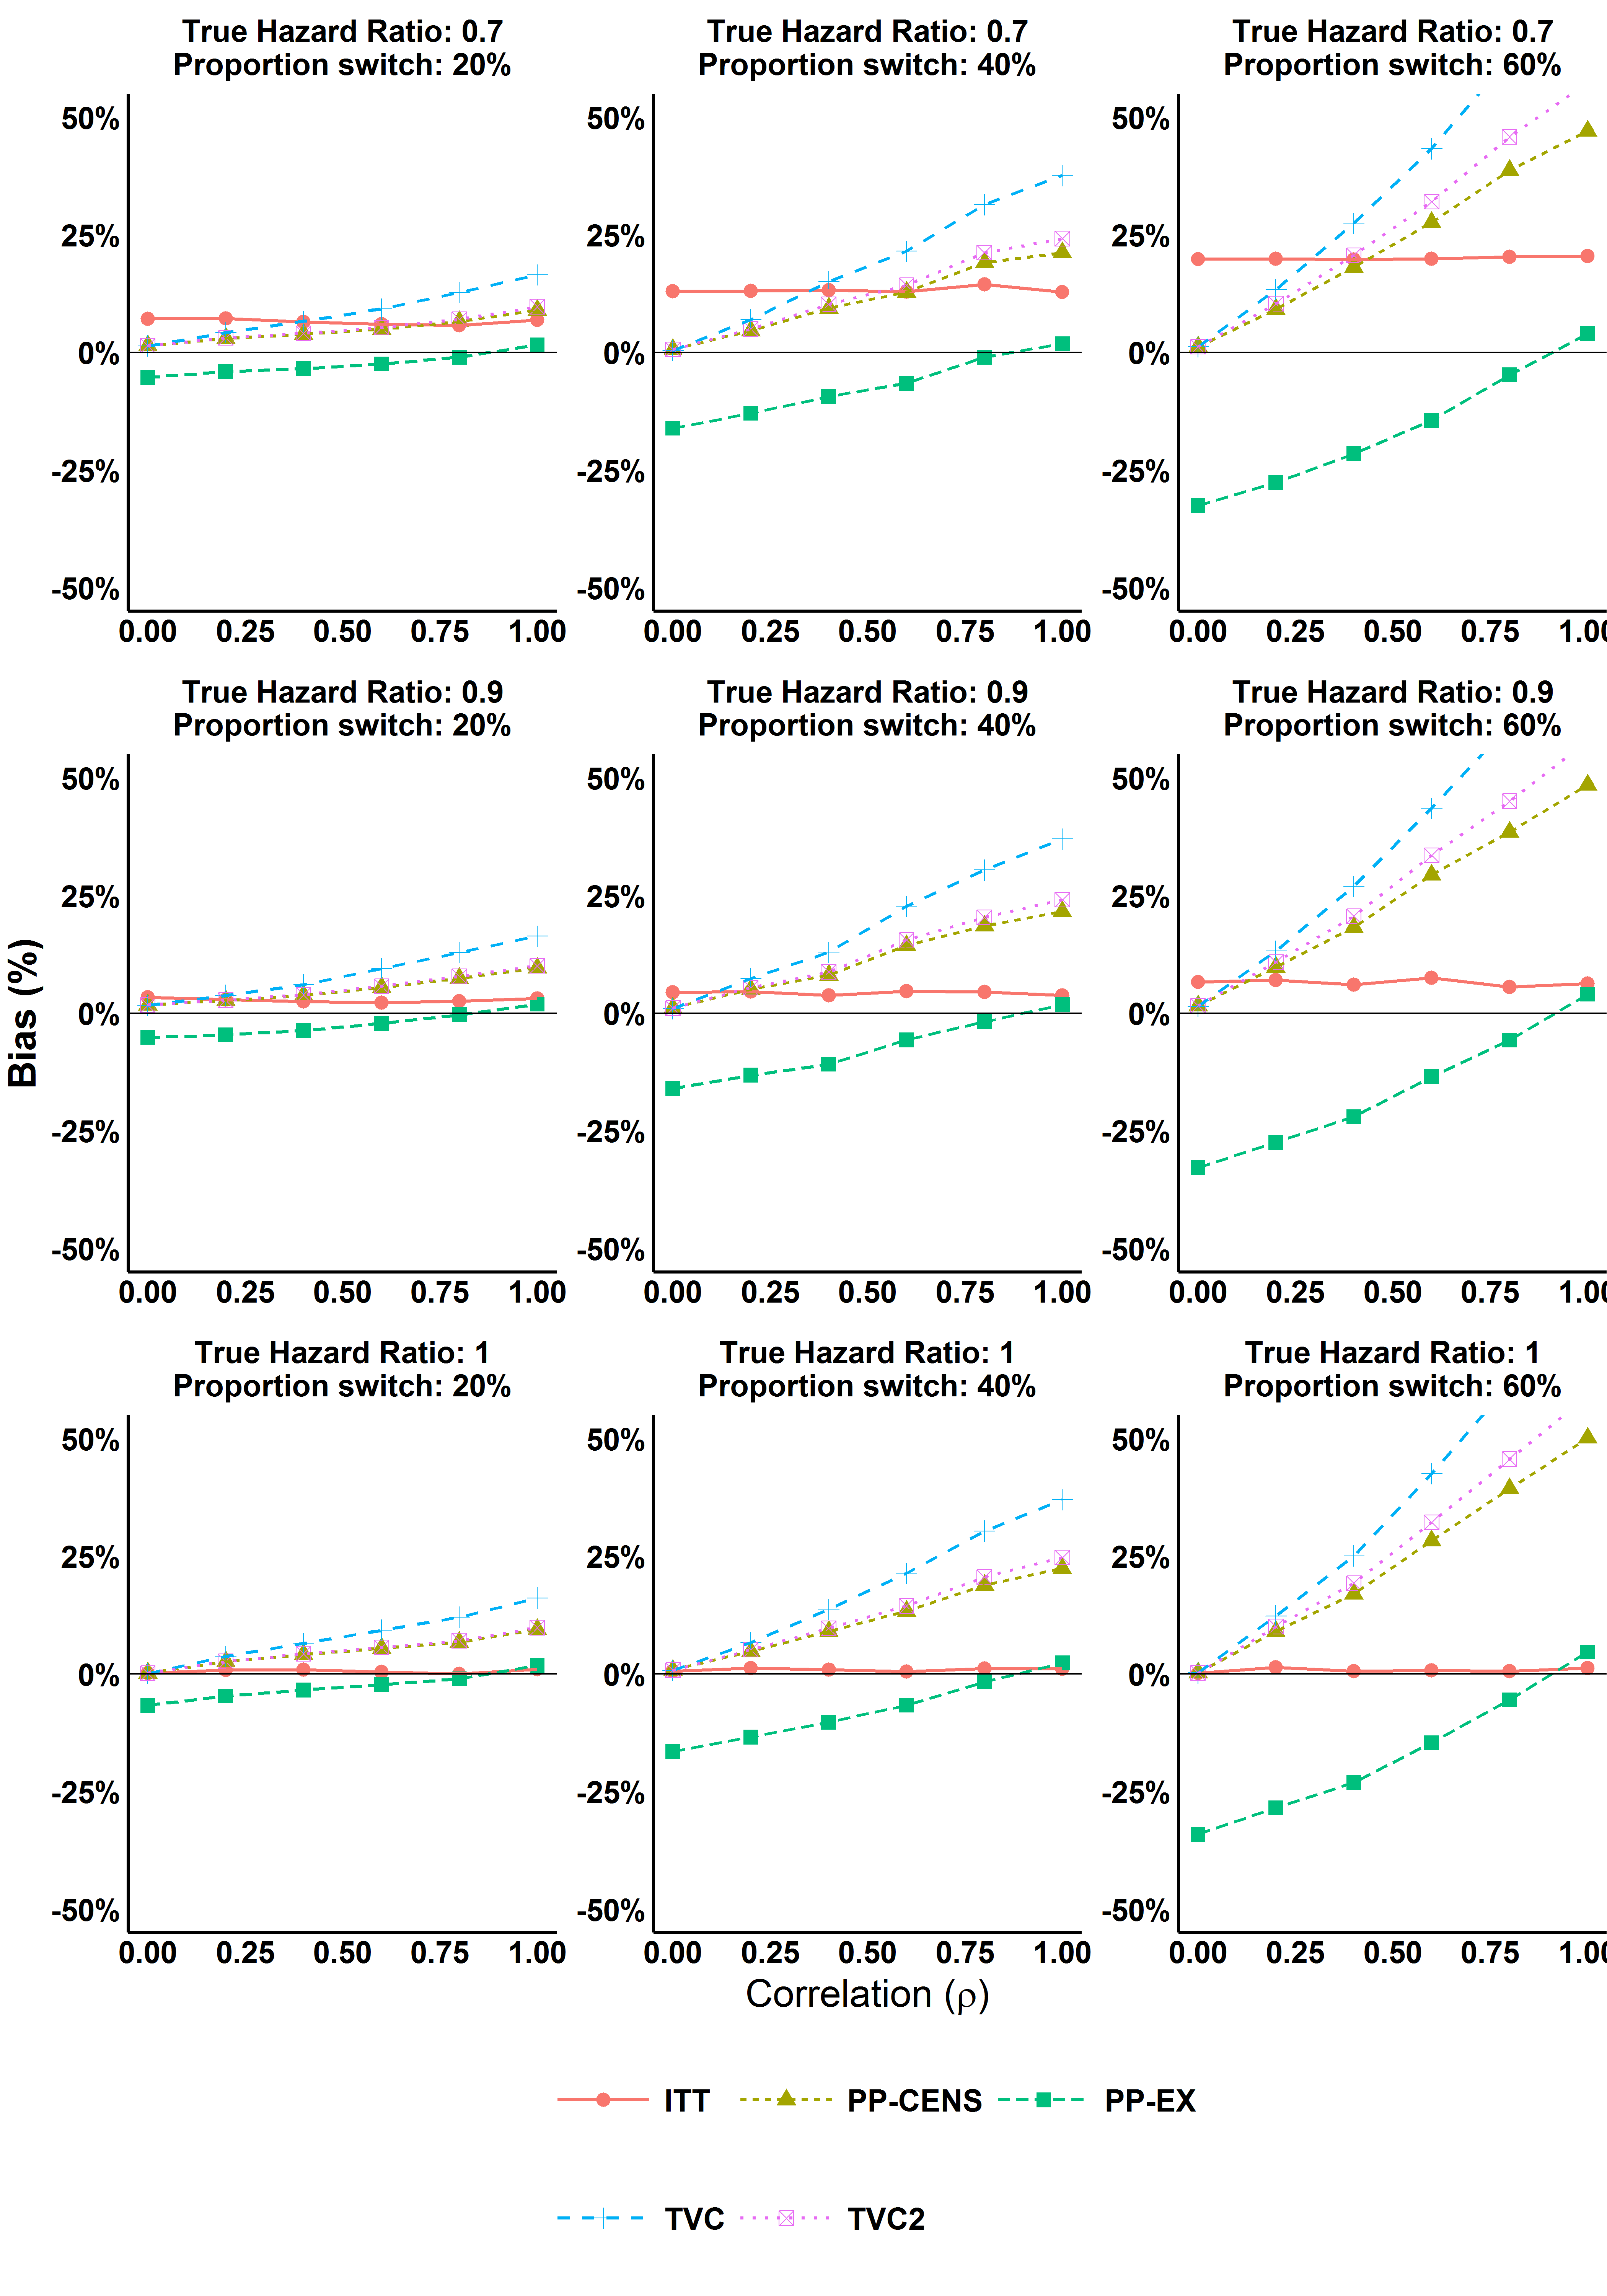
\includegraphics[width=13cm]{images/chap_sim2/simple_bias.png}
\caption{\label{F:chap_sim2:simp_bias} The bias for each of the simple methods across all the scenarios. It can be seen that the bias for ITT is mostly independent of correlation and tends to underestimate the treatment effect. For the Per-protocol Excluding Switch Patients (PP-EX) analysis the bias is large across all correlations and true hazard ratios once the proportion switch is greater than 20\%. For Per-protocol Censoring at Switch (PP-CENS) analysis and both analysis including Treatment as a time-varying covariate (TVC and TVC2) there is minimal bias when there is no correlation between survival and time to progression and very large bias otherwise. } 
\end{figure}

\subsubsection{Complex methods}

For the complex methods in these scenarios the correlation between Time To Progression and Overall Survival doesn't seem to much affect the bias observed as can be seen in Figure \ref{F:chap_sim2:comp_bias} and Figure \ref{F:chap_sim2:2saft_bias}. It can also be seen that the bias is much reduced compared to any of the simple methods regardless of scenario.

For the 6 variations of rank preserving survival time (RPSFT) models considered the choice of test log-rank (RPSFT-LR) or Wilcoxon (RPSFT-W) had negligible impact on the bias as can be seen in Appendix \ref{A:sim2res}. Considering the choice of modelling approach between ``treatment group'' (RPSFT-TG) and ``on treatment'' (RPSFT-OT) in general for this study it can be seen in Figure \ref{F:chap_sim2:comp_bias} the ``treatment group'' approach performed better though this is possibly because this better matches the way the data was generated. Of interest is that where the proportion switching is 40\% or less the ``on treatment'' modelling performs reasonably despite not matching the data generation procedure with bias < 0.05 across these scenarios. It can also be seen from this figure that the choice between estimating a hazard ratio from a comparison of observed and latent (RPSFT-OT-LR-TU) survival times or through using only counterfactual (RPSFT-OT-LR-V) times as discussed in Section \ref{S:chap_methrev:RPSFTestHR} has negligible impact.

For the modified iterative parameter estimation (MIPE) method in general bias was comparable to that of the RPSFT with estimation of the hazard ratio from the weibull parameters (MIPE-WEIB) generally having higher bias than when estimating the hazard ratio from a comparison of latent and observed survival times (MIPE). The exception is the scenarios with true Hazard Ratio of 0.7 and proportion switch of 20\% where it is unclear why the MIPE consistently underestimates the true Hazard Ratio regardless of correlation.

For the two-stage AFT approach the bias in absence of correlation is the same for all four models considered, however, once a correlation between time to progression and overall survival is introduced the model excluding PFS (2SAFT-NULL) has slightly increased bias. It also appears the omitting the recensoring algorithm increases the bias slightly.

\begin{figure}[ht]
\centering
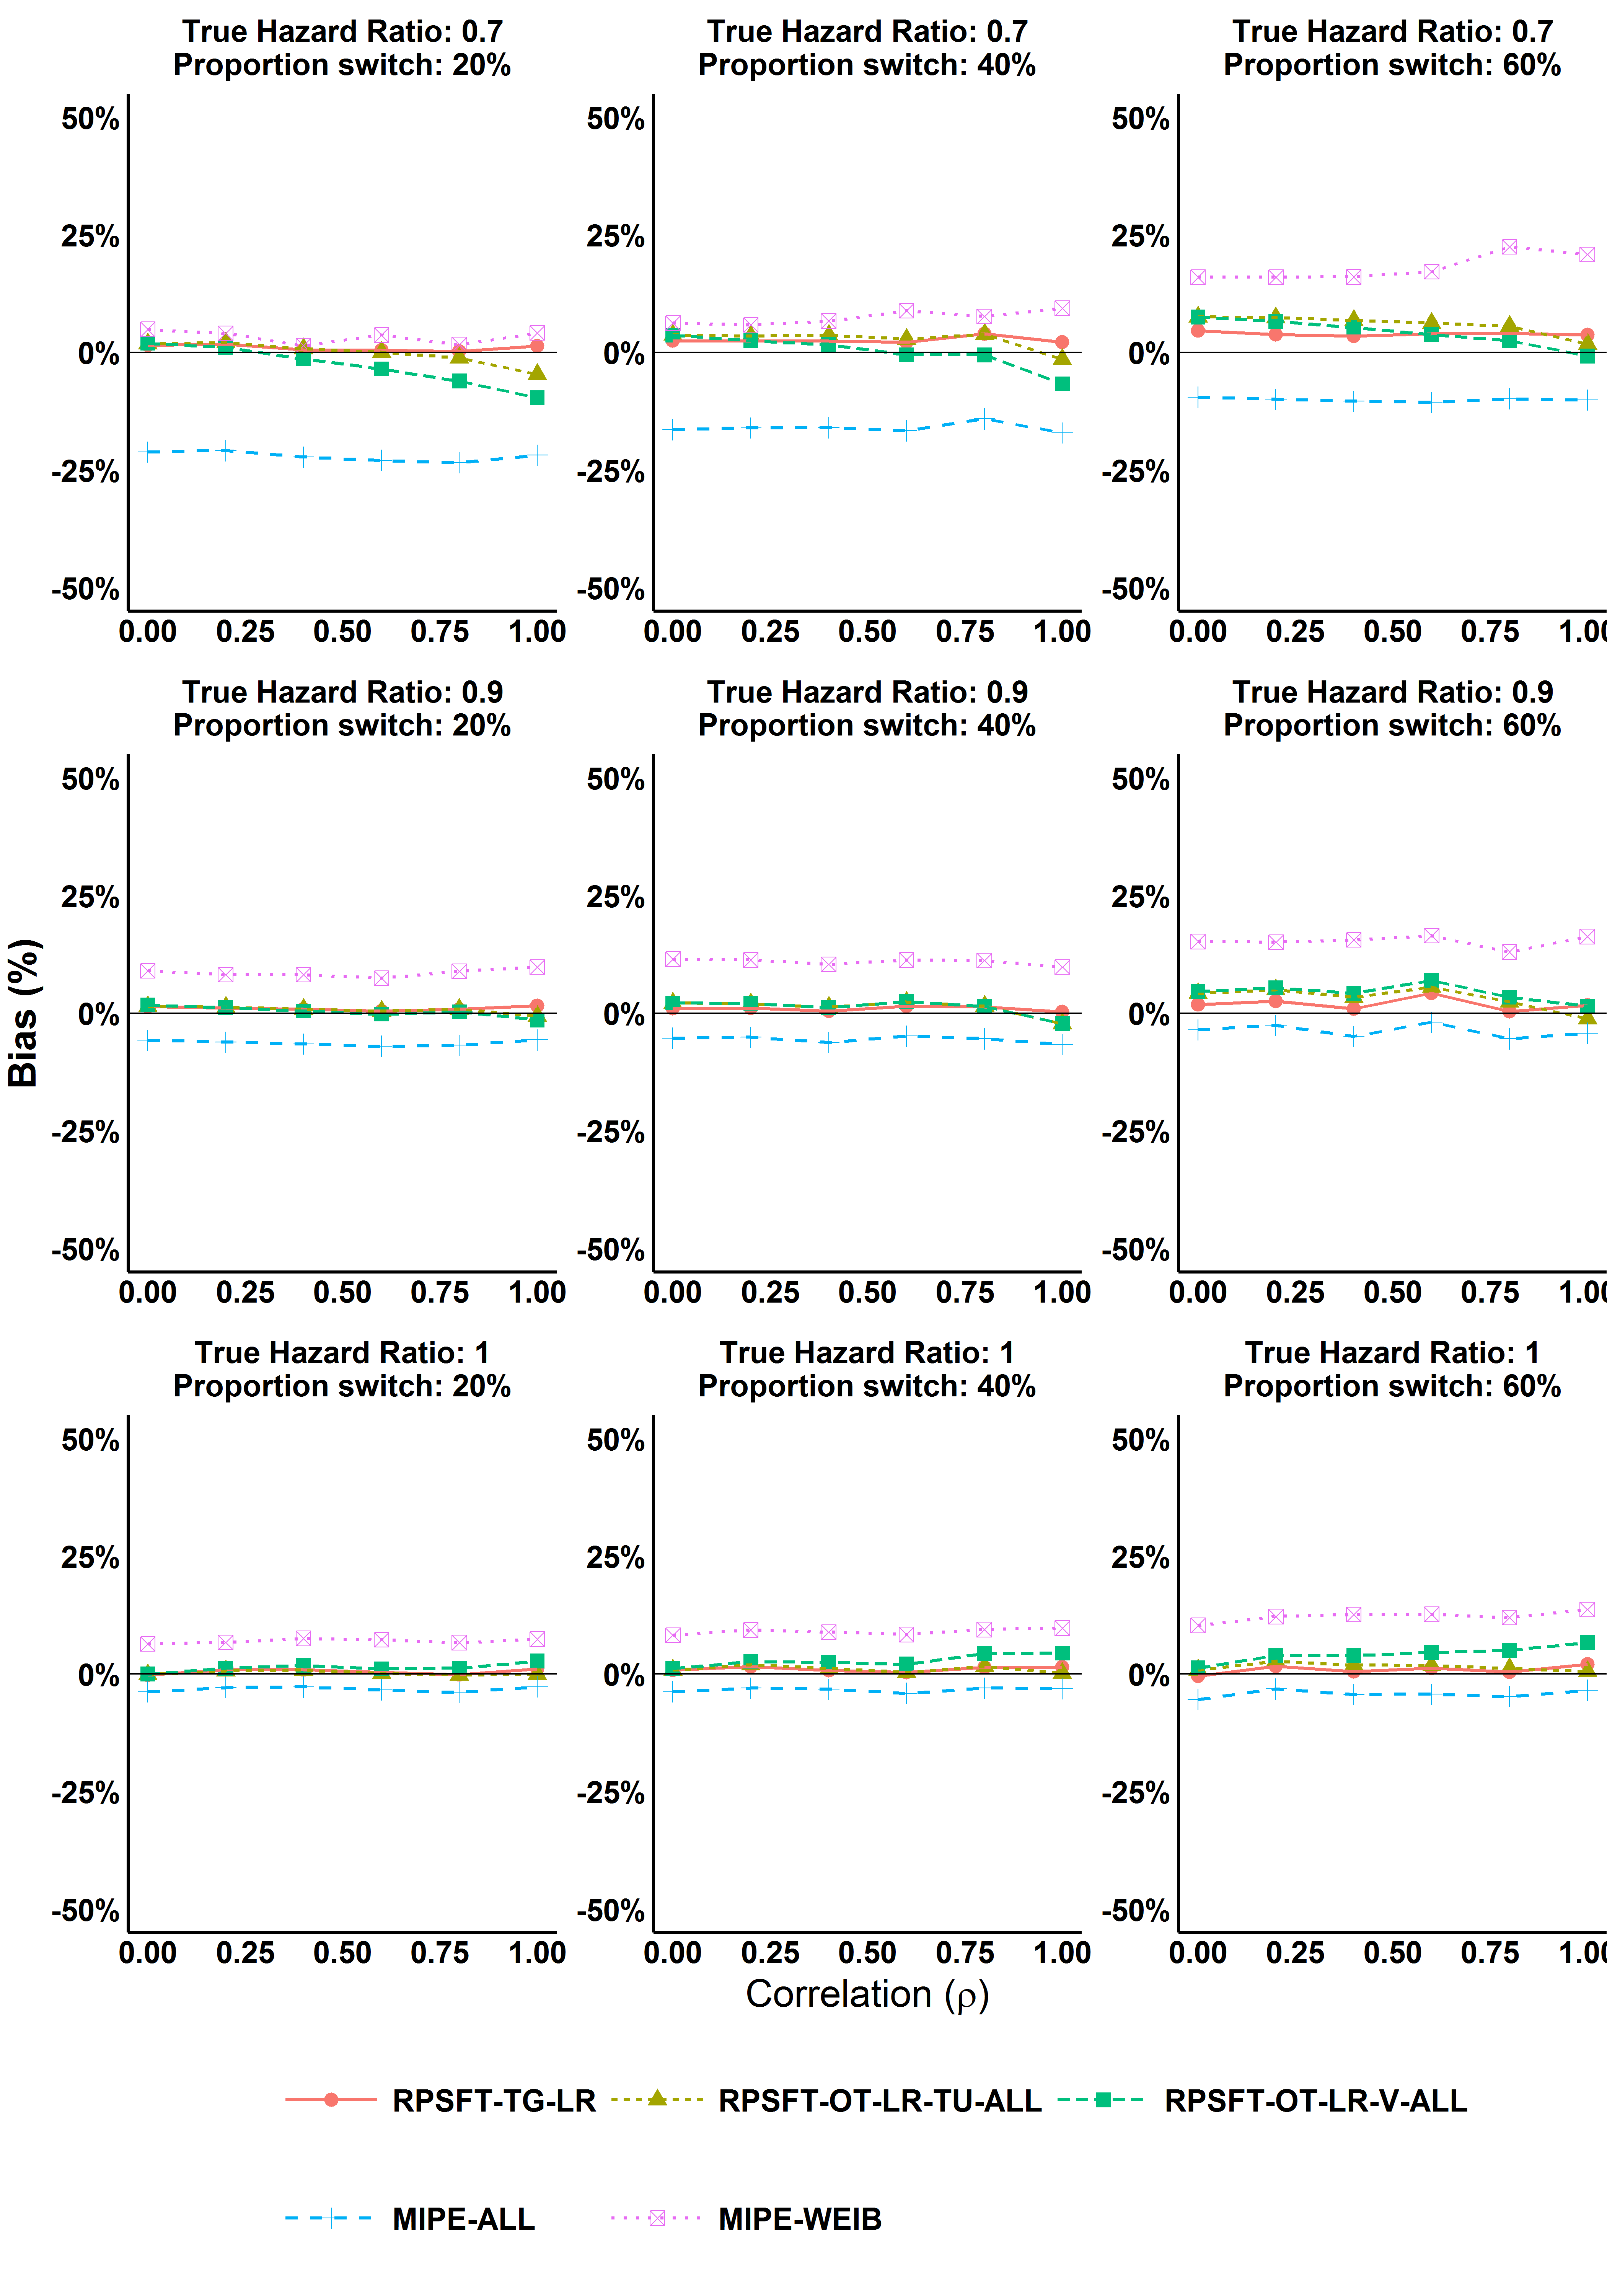
\includegraphics[width=13cm]{images/chap_sim2/complex_bias.png}
\caption{\label{F:chap_sim2:comp_bias} The bias for each of the complex methods across all the scenarios. Compared to the simple methods there is less relationship between correlation, proportion switch and bias. The bias of the Modified Iterative Parameter Estimation (MIPE) appears to depend on the method used to estimate the Hazard Ratio when the true treatment effect is large. For the three variations on RPSFT the absolute bias level is similar.} 
\end{figure}

\begin{figure}[ht]
\centering
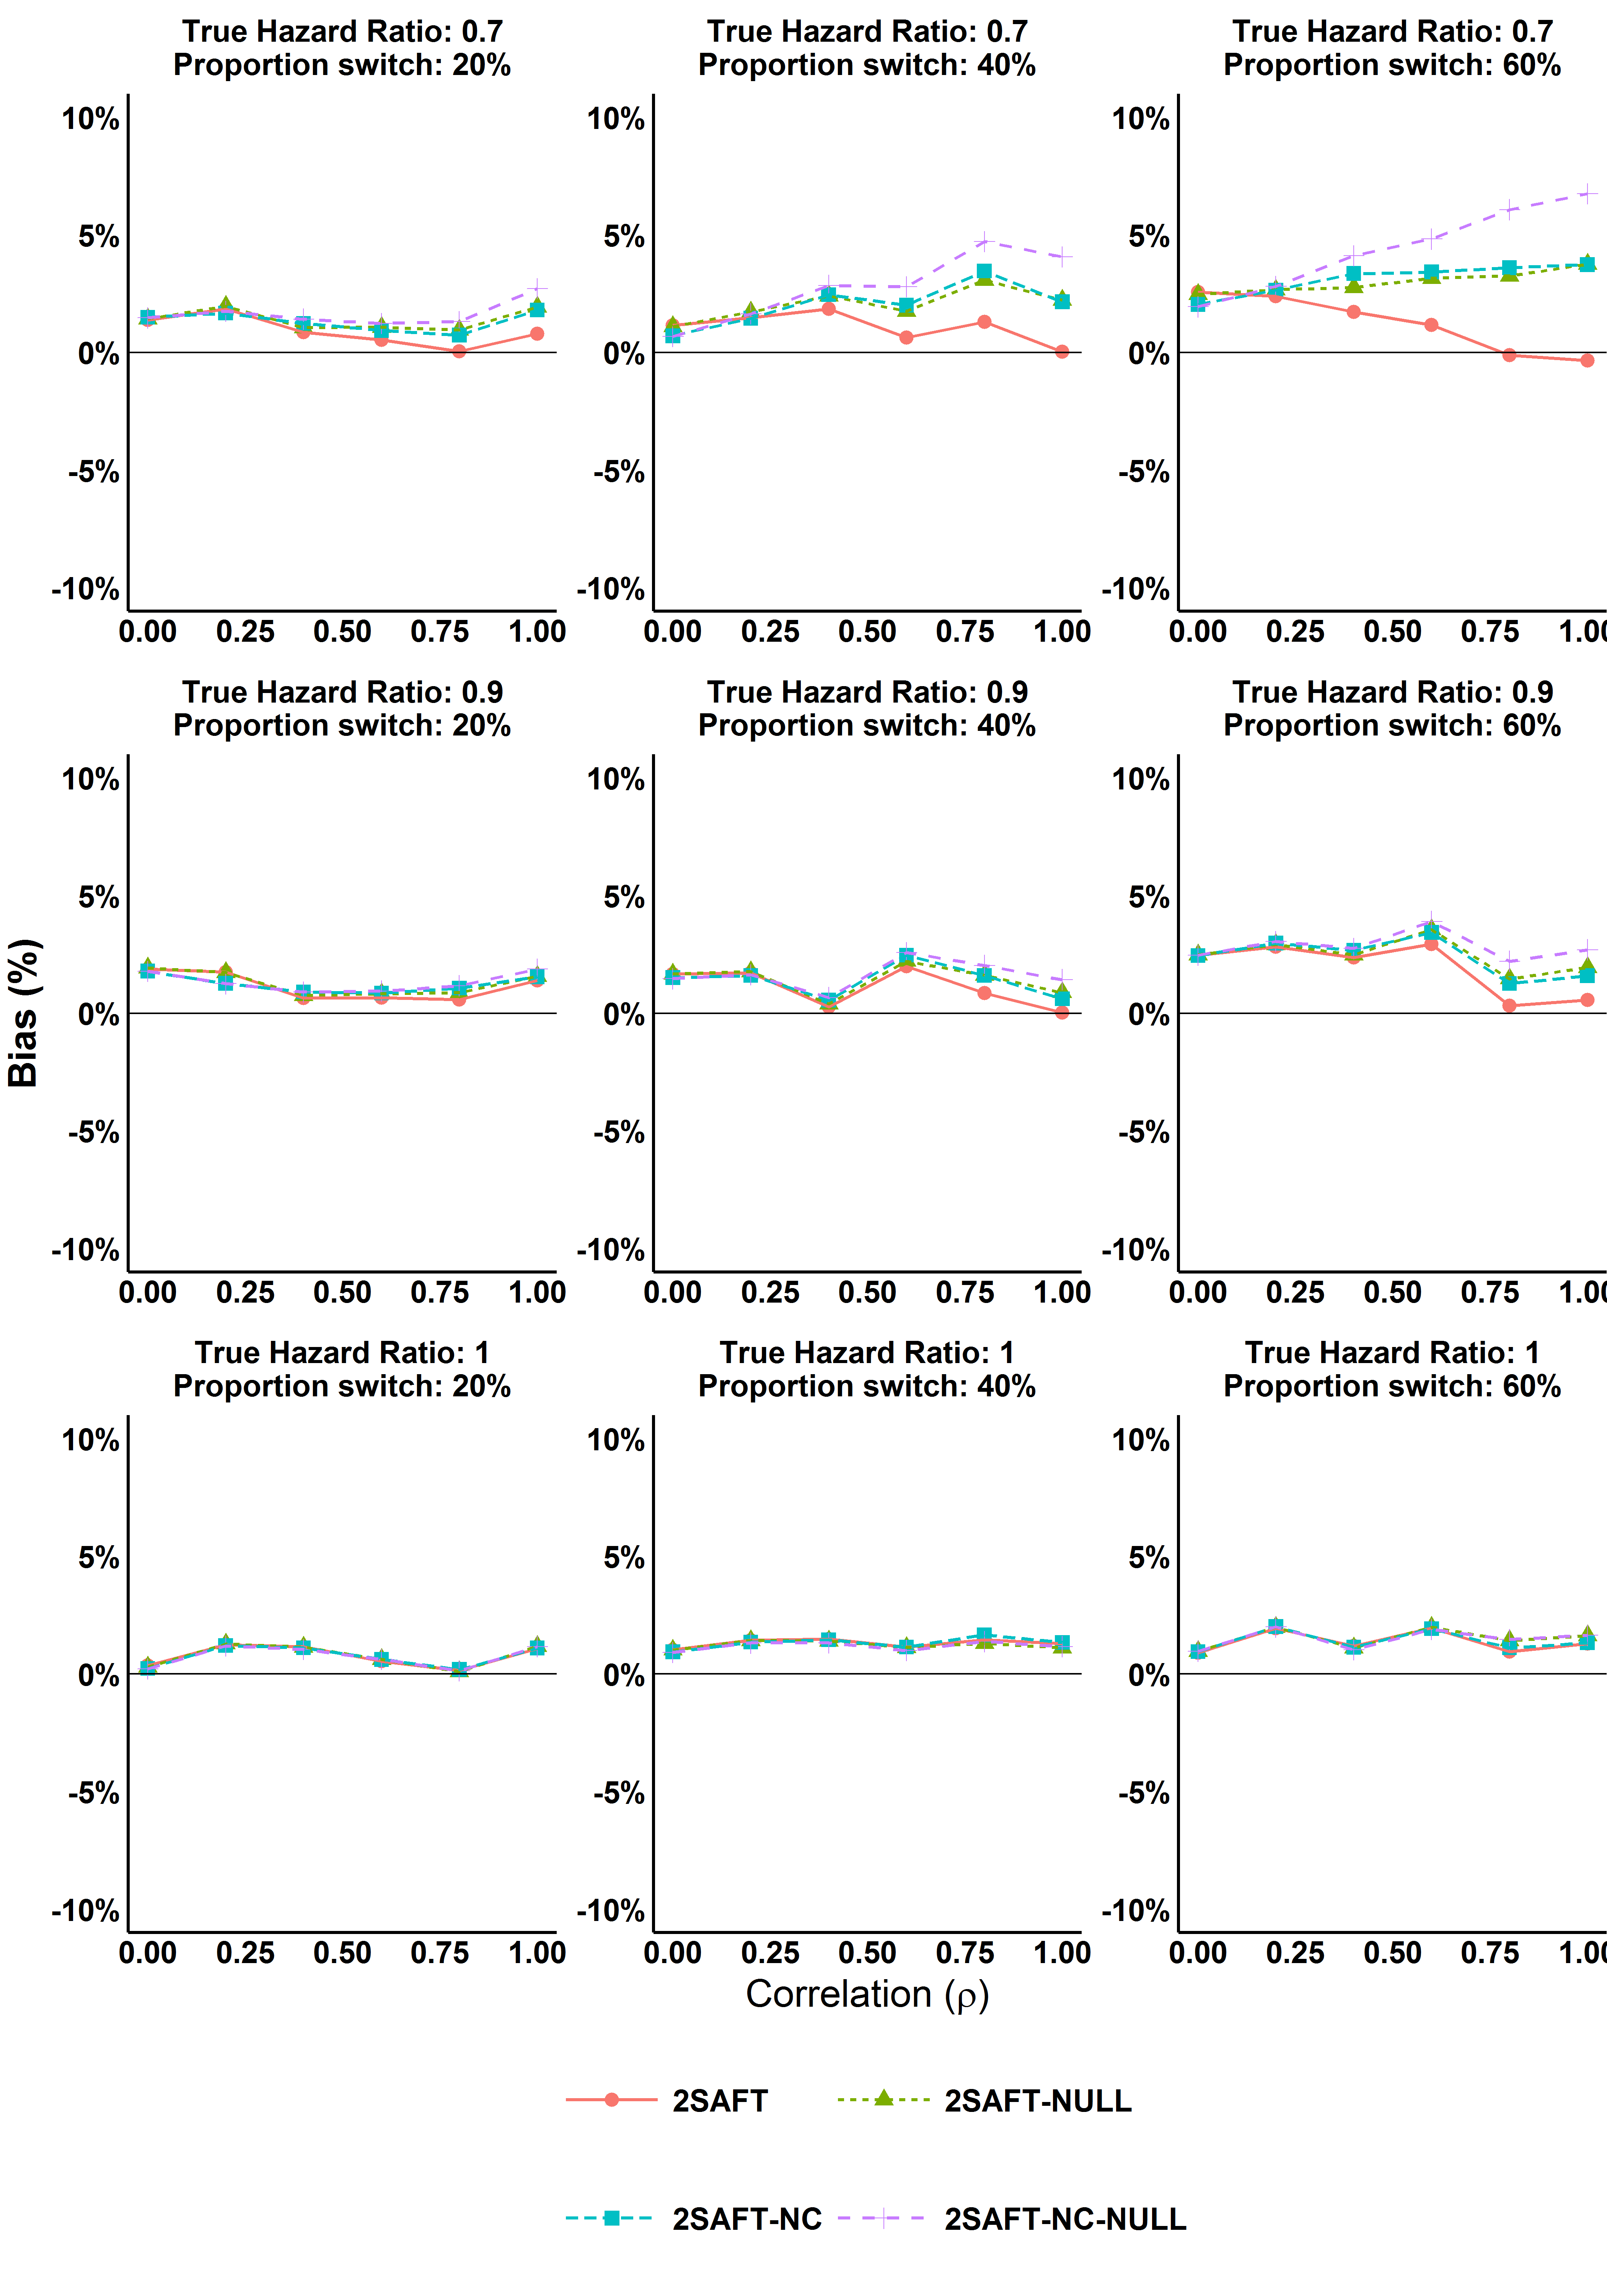
\includegraphics[width=13cm]{images/chap_sim2/2saft_bias.png}
\caption{\label{F:chap_sim2:2saft_bias} The bias for the various approaches to the two-stage AFT method across all the scenarios. The bias is low with no obvious relationship to correlation. NULL indicates that the model for survival post progression includes no covariates while NC indicates that no recensoring is implemented. For scenarios with larger treatment effect the importance of specifying the correct model and re-censoring is increased.} 
\end{figure}


\clearpage

\subsection{Coverage}

Figure \ref{F:chap_sim2:simp_cov} and Figure \ref{F:chap_sim2:comp_cov} show the coverage for the simple and complex methods respectively. It can be seen that the estimated confidence intervals from the Time varying covariate method (TVC) and per-protocol censoring at switch analysis (PP-CENS) have very poor coverage with even moderate levels of correlation. For the ITT method the lowest coverage is 76.8\% with coverage being worse with larger proportions of switching. When the true Hazard Ratio is 1.0 the coverage is stable between 93.9\% to 96.5\%.

For the per-protocol analysis excluding switchers (PP-EX) the coverage is poor across all scenarios and is often <50\% where the proportion who switch is 60\%.

For all the variations of RPSFT the 95\% confidence intervals are estimated using the correction described in Section \ref{S:chap_methrev:RPSFTestHR} and as can be seen in Table \ref{T:chap_sim2:simres} and Figure \ref{F:chap_sim2:comp_cov} the coverage for all scenarios is very stable for the ``treatment group'' (RPSFT-LR-TG) ranging from 90.5\% to 96.8\% across all 54 scenarios investigated. Similarly to the findings for bias the ``on treatment'' approach (RPSFT-LR-OT) tends to perform worse, however, the lowest coverage across all 54 scenarios was 82.0\% which is favourable compared to any of the simple methods and bootstrapping is likely required. As expected the MIPE method had some scenarios with very low coverage and it is clear that bootstrapping of confidence intervals is required. For the two-stage AFT the coverage is much improved from the simple methods but it is clear that bootstrapping is required when considering the scenarios where there truly is no treatment effect (Hazard Ratio = 1) and coverage can be as low as 82\%.


\begin{figure}[ht]
\centering
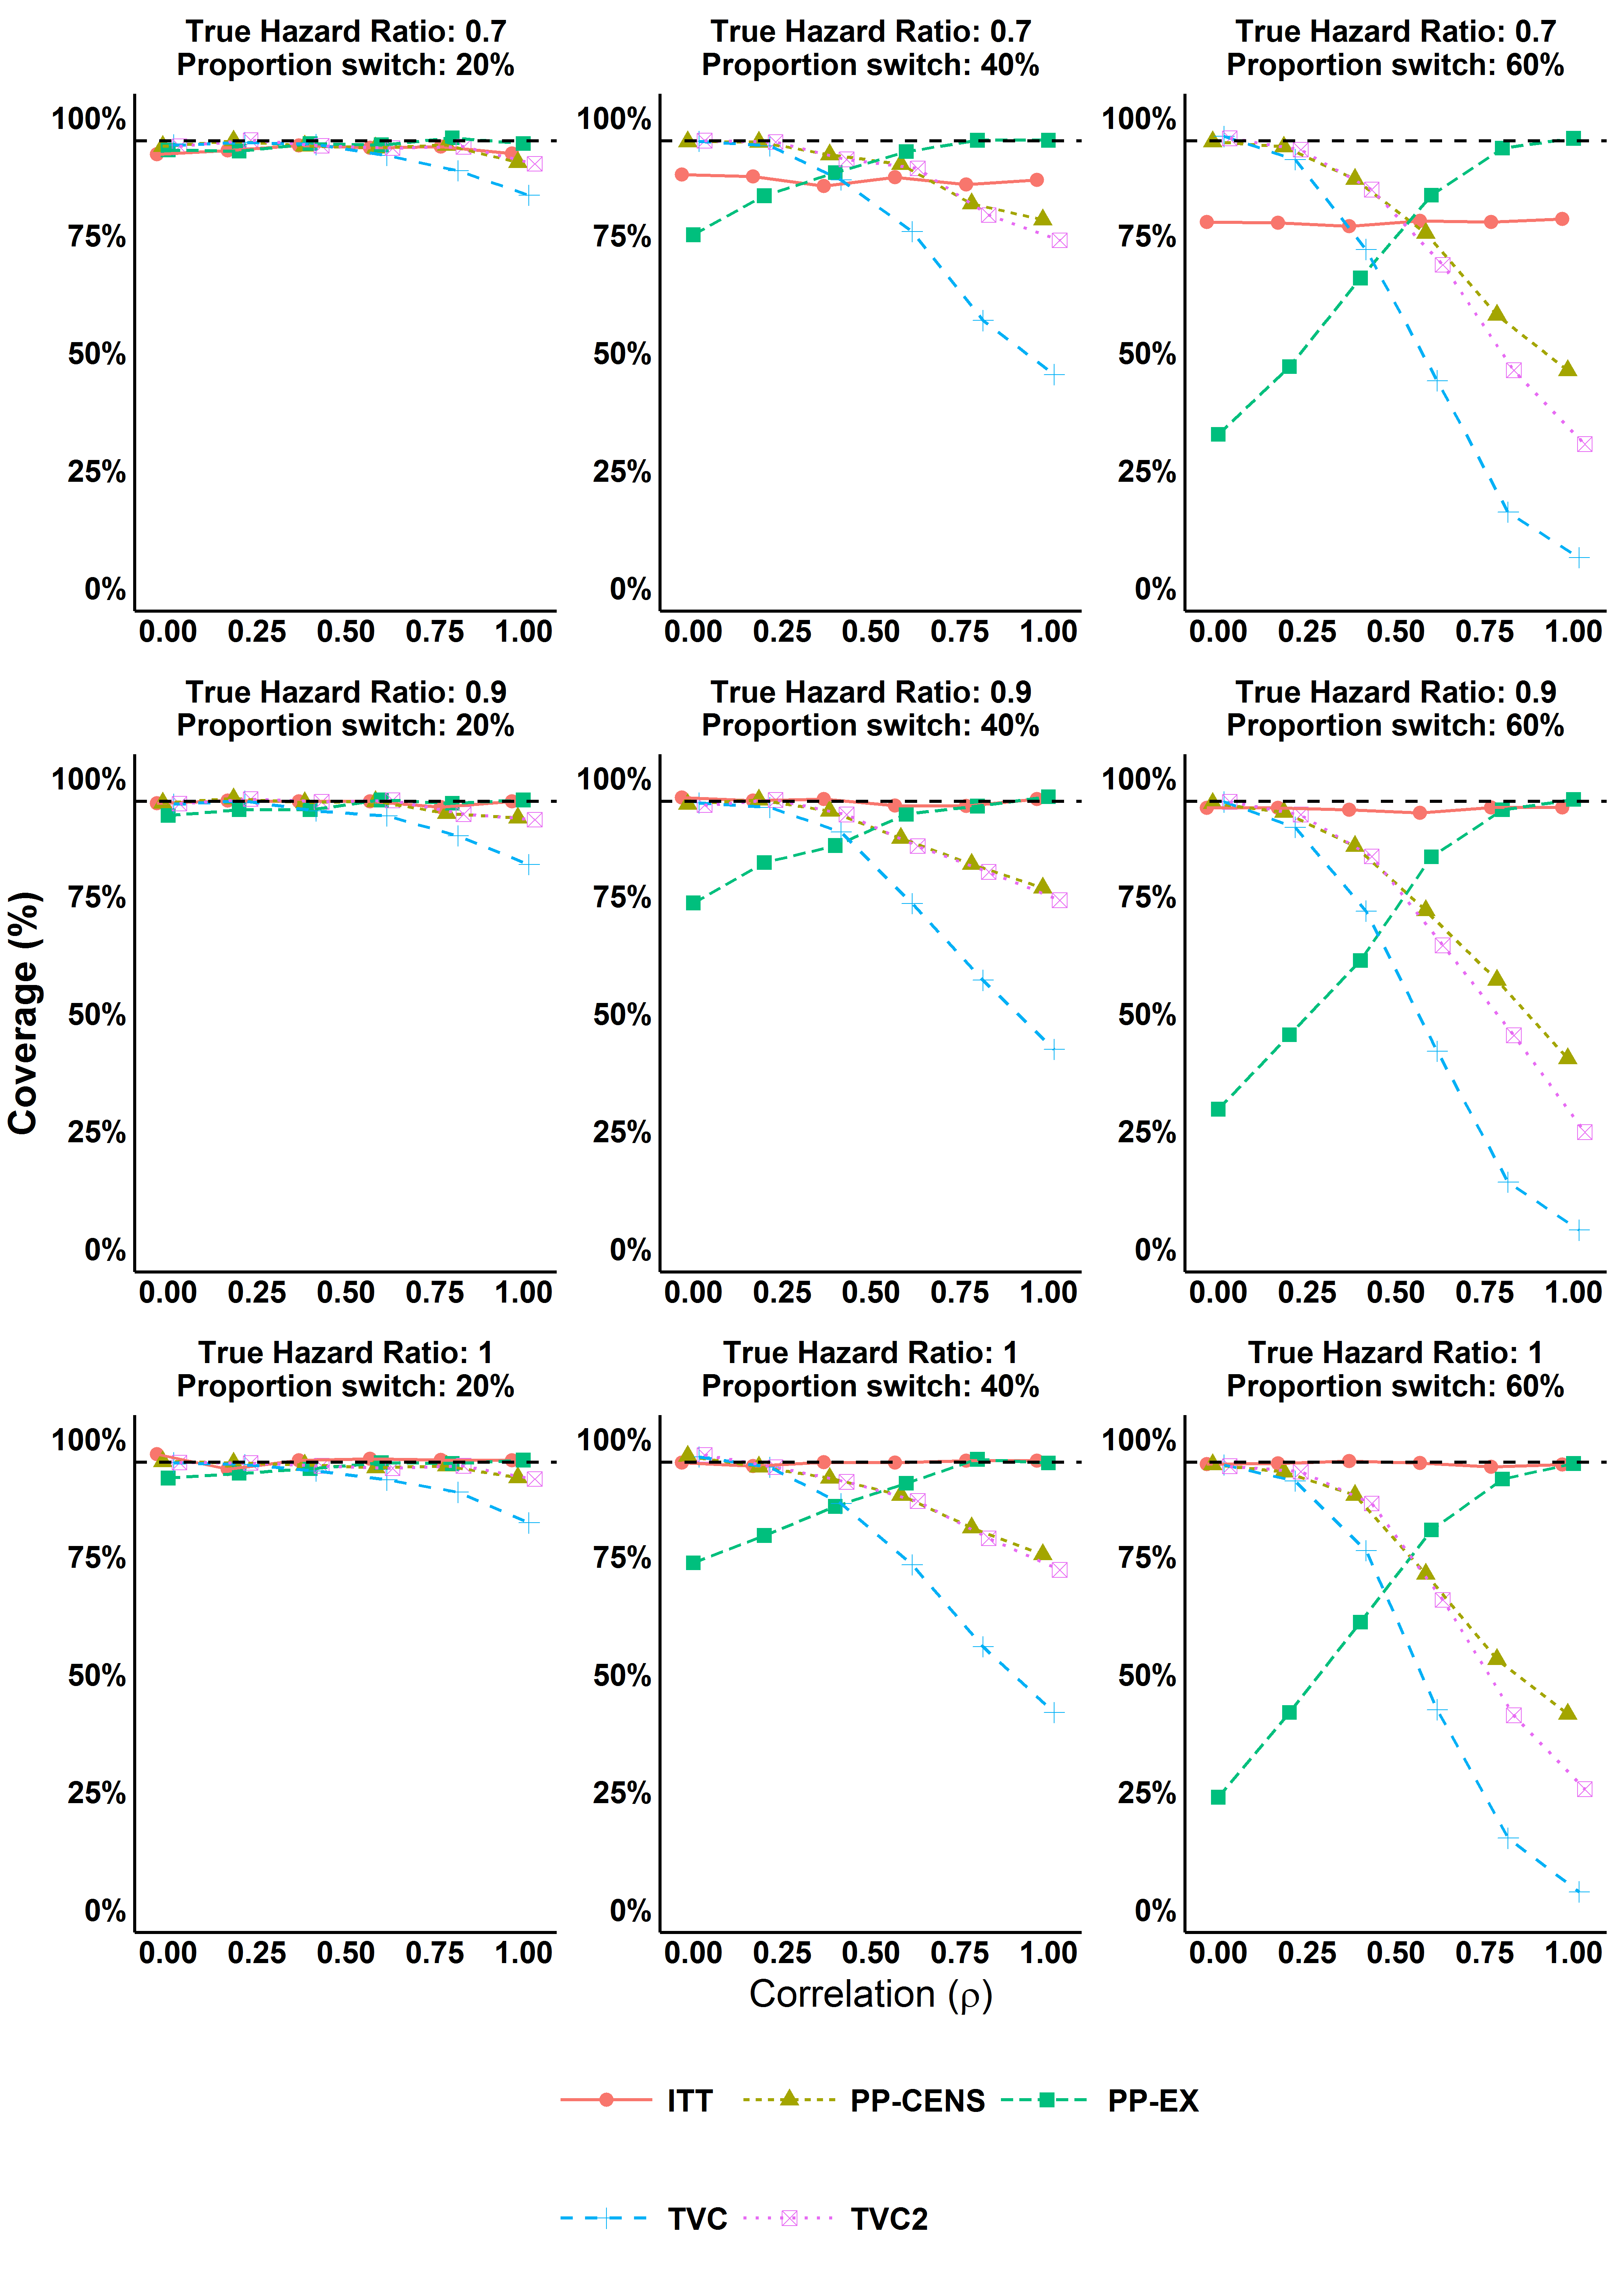
\includegraphics[width=13cm]{images/chap_sim2/simple_cov.png}
\caption{\label{F:chap_sim2:simp_cov} The coverage for each of the simple methods across all the scenarios. As with bias the performance of Censoring at switch (PP-CENS) and inclduing a time varying treatment covariate (TVC) is strongly related to correlation and very poor unless there is no correlation between TTP and OS. The method of excluding switchers (PP-EX) performs badly across every scenario except where the proportion of control patients switching is low.} 
\end{figure}

\begin{figure}[ht]
\centering
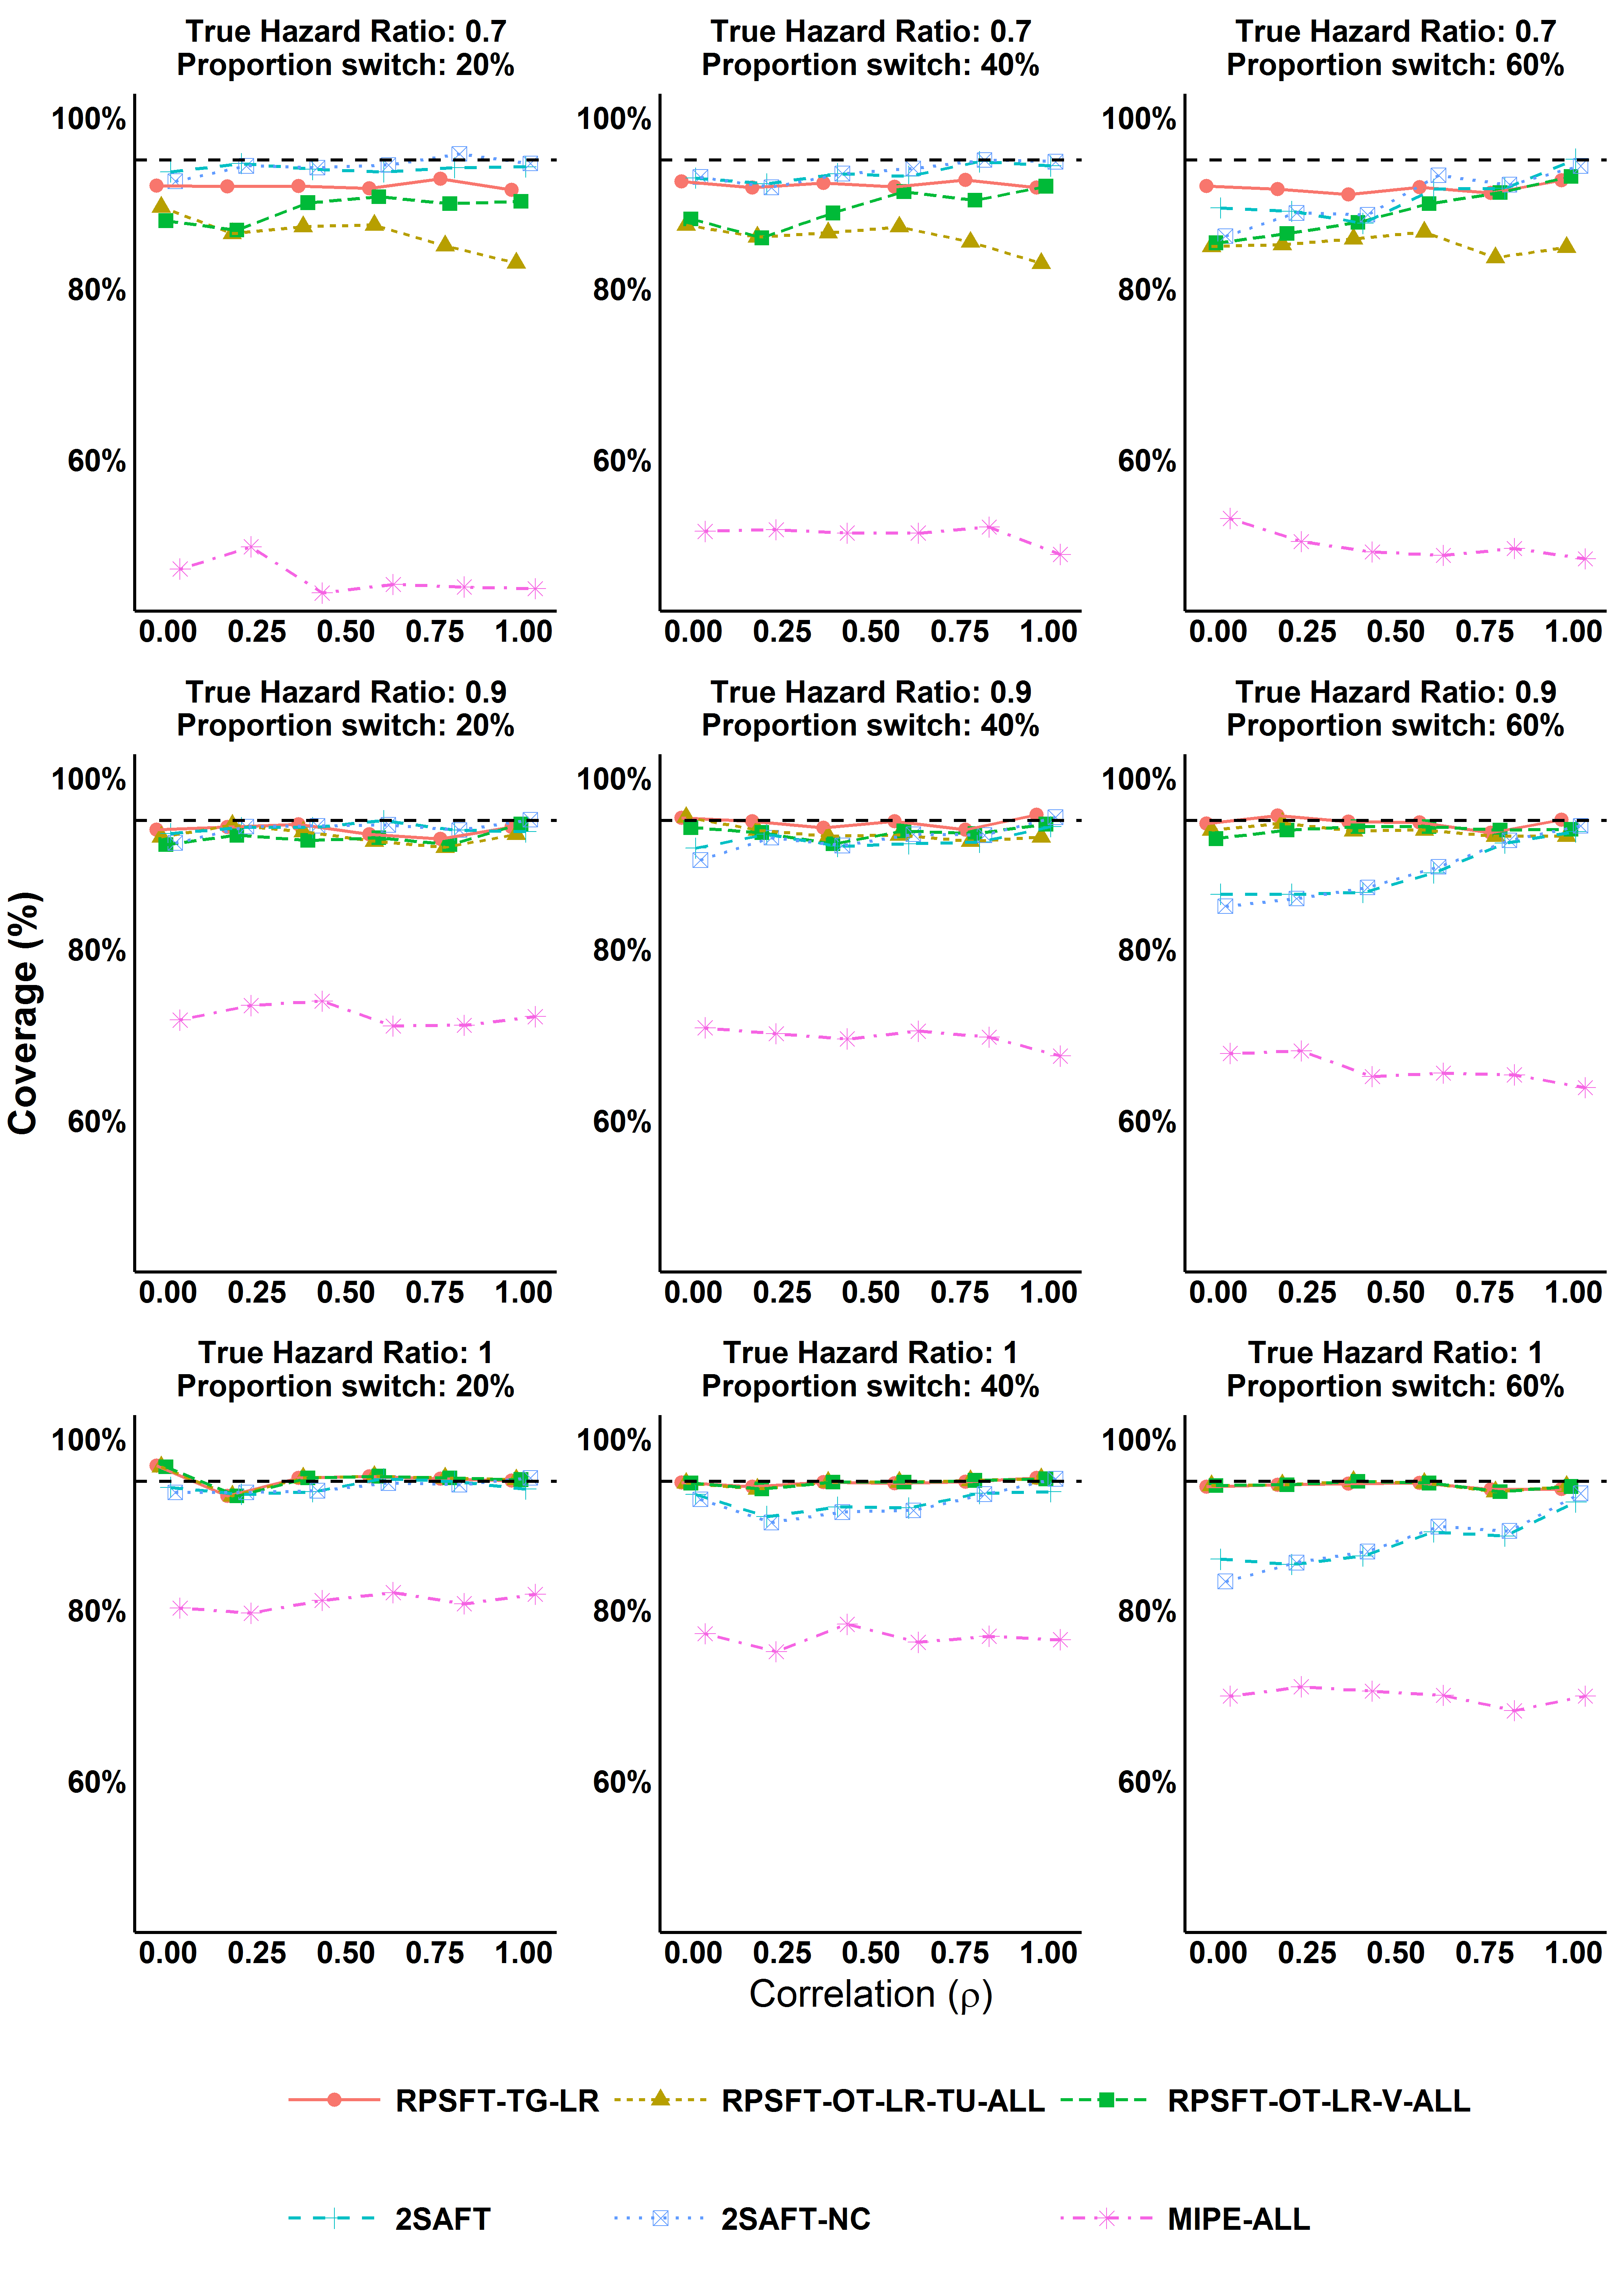
\includegraphics[width=13cm]{images/chap_sim2/complex_cov.png}
\caption{\label{F:chap_sim2:comp_cov} The coverage for each of the complex methods across all the scenarios. As expected bootstrapping of confidence intervals is needed for the MIPE and two-stage AFT (2SAFT) method with coverage poor particularly for scenarios where there is no treatment effect (True HR=1). The test-based correction proposed by \cite{White1999} performs reasonably but where there is a large treatment effect bootstrapping should be preferred.} 
\end{figure}

\clearpage 

\subsection{Convergence}
\begin{figure}[h!]
\centering
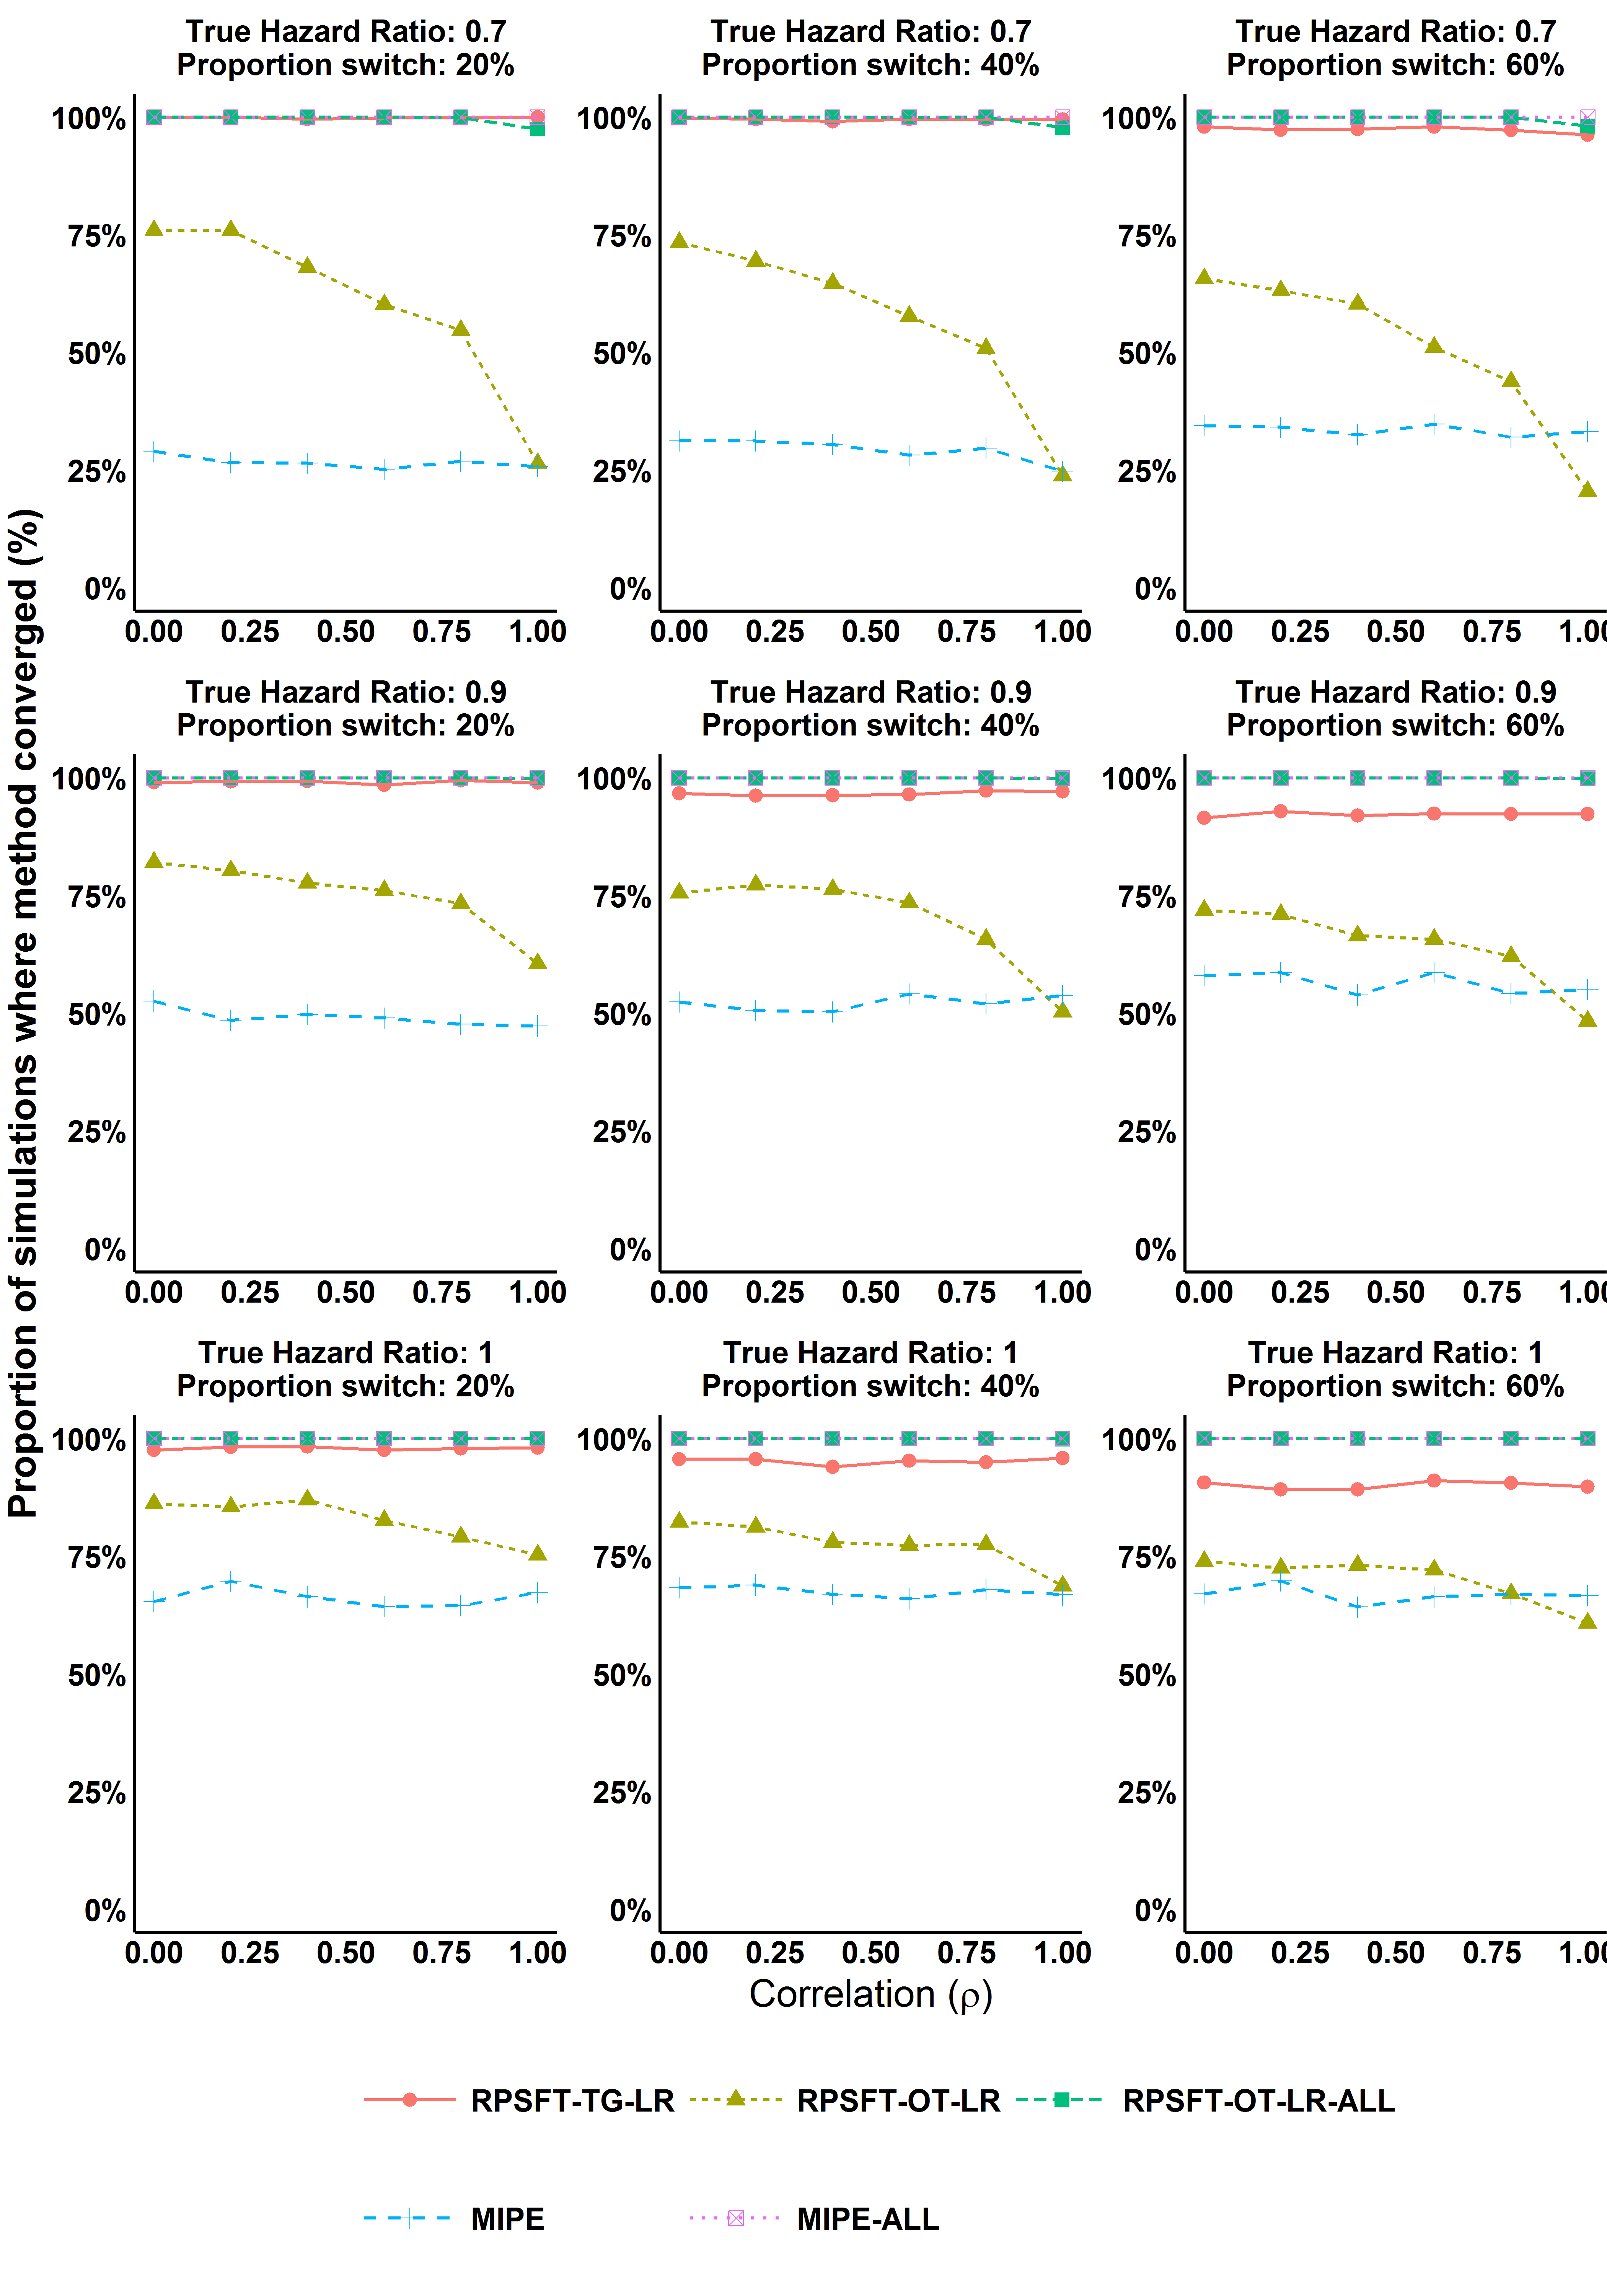
\includegraphics[width=13cm]{images/chap_sim2/complex_conv.png}
\caption{\label{F:chap_sim2:comp_conv} This figure shows the proportion of simulations where the complex methods rank-preserving failure time (RPSFT) and modified iterative parameter estimation (MIPE) converged to a unique solution. For the ``treatment group'' approach (RPSFT-LR-TG) convergence was high across all scenarios. For the ``on treatment'' approach (RPSFT-LR-OT) and MIPE the convergence was quite poor when the proportion of switch was high, the treatment effect was large or there was a large correlation between time to progression (TTP) and survival (OS). By using imputation approaches the convergence is improved to nearly 100\% for both RPSFT and MIPE (RPSFT-LR-OT-ALL, MIPE-ALL).}
\end{figure}

In Table \ref{T:chap_sim2:simres} and Figure \ref{F:chap_sim2:comp_conv} it can be seen that the complex methods sometimes fail to converge. The ``treatment group'' approach to rank-preserving failure time (RPSFT-LR-TG) modelling performed best with a lowest convergence across all scenarios of 89.2\%. This compares to the  ``on treatment'' approach (RPSFT-LR-OT) where for one scenario a unique solution was only found for 20.5\% of simulations and 24.8\% for the modified iterative parameter estimation (MIPE) method. When the imputations discussed in Section \ref{S:chap_sim2:convimp} the convergence can be increased dramatically for both approaches. Figure \ref{F:app_sim2:compA_bias} and Figure \ref{F:app_sim2:compA_cov} in Appendix \ref{A:sim2res} show that these imputations do not dramatically change the bias or affect the coverage of these methods and in the case of scenarios where convergence is very low they are beneficial. As the primary benefit of MIPE is an improved estimation algorithm this convergence performance is disappointing given the need to make additional assumptions over the RPSFT approach.


\clearpage

\section{Conclusion from simulation study 1}

In this simulation study the main parameter varied was the correlation between time to progression and overall survival. As observed in the simulation study from \cite{Morden2011} the ITT method underestimates the true treatment effect with the direction of bias being predictable regardless of correlation induced. Replicating the findings of \cite{Morden2011} it appears that both per-protocol analyses (censoring at crossover and excluding switchers) perform quite badly when a correlation is induced between time to progression and overall survival as the probability of switching is then dependent on prognosis. This is also the case of the approach of using a time-varying covariate in the cox model to estimate treatment effect. All of these methods appear to yield biased estimates when time to progression and overall survival times are correlated. 

As seen with the simulation study from \cite{Morden2011} the RPSFT method perform well regardless of correlation and flavour implemented. However, for MIPE the bias is in some scenarios larger than observed with the RPSFT which combined with the fact that convergence is worse than the ``treatment group'' approach to RPSFT and not consistently better than the ``on treatment'' approach means the value of this method seems limited given the need to make additional parametric assumptions.

The two-stage AFT method performs quite well in this simulation study showing similar bias to that seen with the ``treatment group'' approach to RPSFT when the model is correctly specified and recensoring is implemented. If the model is incorrectly specified by not including progression free-survival time then the bias is increased but is still lower than any of the simple methods considered here.


\chapter{Simulation Study 2}
\label{C:chap_sim3}

This Simulation study again uses the framework described in Chapter \ref{C:chap_sim_design} but compared to Chapter \ref{C:chap_sim2} more complex patterns of treatment effect are considered. The main objective of this simulation study is to investigate the sensitivity of the RPSFT and MIPE methods to violations of the common treatment effect assumption in the presence of correlated survival times.

\section{Study design}

Table \ref{T:chap_sim3:scenarios} shows a summary of the scenarios investigated and parameters for treatment effects (as defined in Chapter \ref{C:chap_sim_design}). For each of the 6 scenarios investigated $\rho$, the correlation between Time to Progression and Overall Survival, is varied across 6 levels from 0 to 1 and the proportion of patients who switch is set at 40\% and 60\% leading to 72 scenarios in total. For each of these 72 scenarios 1000 datasets are simulated. 

\begin{table}[ht] 
\caption{Treatment effect scenarios for simulation study 2}
\centering 
\begin{tabular}{ l l r r r r}
\hline
\hline
Description & ID & \multicolumn{4}{c}{Treatment effects} \\
         &             & \multicolumn{2}{c}{Experimental arm} & \multicolumn{2}{c}{Control arm} \\
%         &             & during    & after      & during     & after     \\
		 &             & $\exp(\beta_{1a})$ & $\exp(\beta_{1b})$ & $\exp(\beta_{2a})$ & $\exp(\beta_{2b})$ \\
\hline
Common effect during treatment      & 1 & $0.5$ & $0.8$ & $0.5$ & $0.8$ \\
with reduced effect after treatment & 2 & $0.8$ & $0.95$ & $0.8$ & $0.95$ \\            
\\
Common effect during treatment     & 3 & $0.01$ & $1$ & $0.01$ & $1$ \\
with no effect after treatment     & 4 & $0.4$  & $1$ & $0.4$ & $1$ \\
\\
Lower effect of switch treatment & 5 & $0.7$ & $0.7$ & $0.8$ & $0.8$ \\
sustained after treatment        & 6 & $0.7$ & $0.7$ & $0.9$ & $0.9$ \\
\hline
\end{tabular} 
\label{T:chap_sim3:scenarios}
\end{table}



\subsection{Rationale for scenarios}

The scenarios 1-4 considered here are meant to represent a treatment effect where a greater reduction on risk of death is received during treatment than after treatment. In scenarios 1 and 2 some residual treatment effect remains after progression and treatment discontinuation whereas for scenarios 3 and 4 there is no residual treatment effect after progression/discontinuation. While at first glance it may appear these scenarios satisfy the common treatment effect assumption of the RPSFT and MIPE method this is not the case as these treatment effects as a reduction in hazard do not translate to a single treatment effect as an acceleration factor. 

Scenarios 5 and 6 are explicitly designed to violate the assumptions of the RPSFT and MIPE approaches in that the treatment benefit received by switch patients are lower than that received by patients receiving randomized treatment. These represent scenarios where patients who have progressed may have a lower capacity to benefit from treatment.

\subsection{Defining a true hazard ratio}


It can be seen that for this simulation study defining the true hazard ratio is problematic for scenarios 1-4 due to the time dependent nature of the treatment effects. To address this the approach of \cite{Latimer2016} is taken and for each of these scenarios 500'000 control and 500'000 experimental patients are generated without switching with the result of this comparison taken as the true value that estimates will be compared against. These ``true'' estimates and the relationship with the correlation between time to progression and overall survival are shown in Figure \ref{F:chap_sim3:truehr}. In these cases what is termed the true hazard ratio is really an average hazard ratio over the observation time of the simulated trial. 

While this approach of defining the ``true'' estimate that the methods are compared against will be prone to some error with the large number of patients used this error should be minimal. A more serious criticism of these scenarios is the use of a Cox model to estimate an average hazard ratio for data where the proportional hazards assumption is clearly violated. Indeed \cite{Schemper1992} show that the Cox model is likely to underestimate the true average hazard ratio in these scenarios even ignoring the problem of treatment switching. Despite this the scenarios are still interesting as what is being examined is how close the proposed methods come to the estimate of hazard ratio that would have been seen without switch. 

\begin{figure}[ht]
\centering
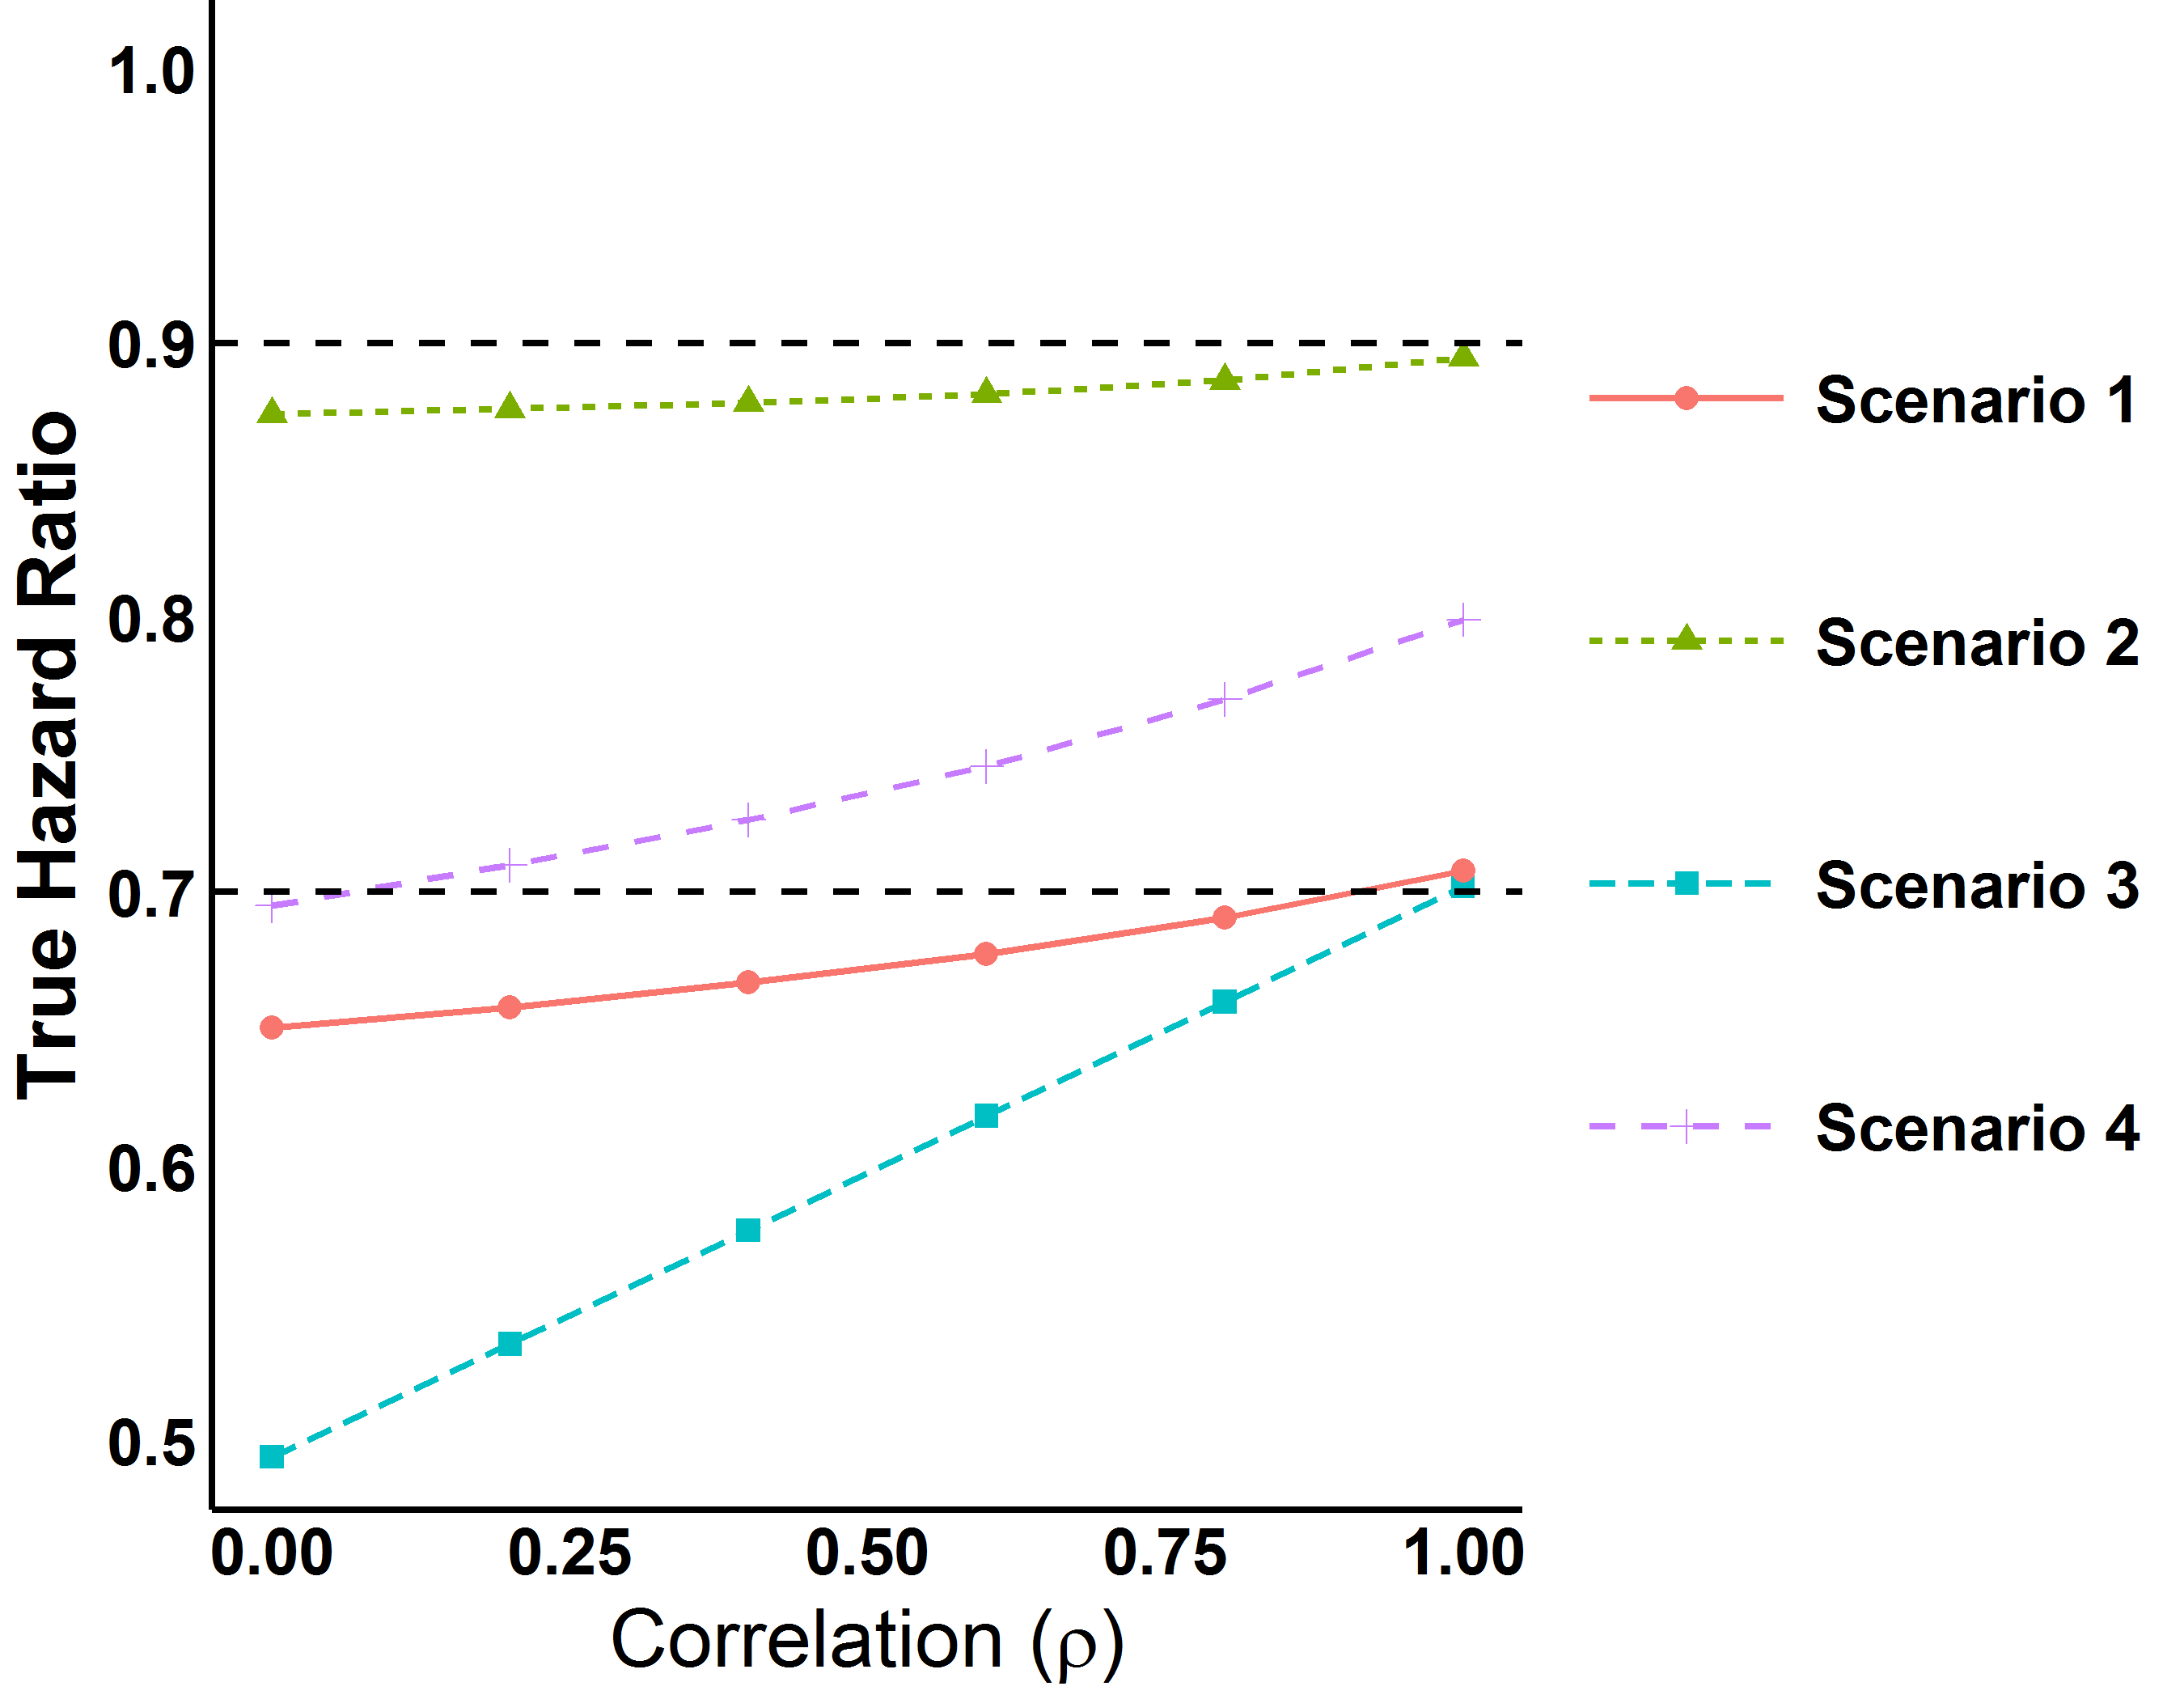
\includegraphics[width=9cm]{images/chap_sim3/truehr.png}
\caption{\label{F:chap_sim3:truehr}  As the application of treatment effects for Scenario 1, 2, 3 and 4 is time dependent the ``true'' average hazard ratio, i.e. that which would be seen if switching did not occur, is estimated using a comparison of 500'000 simulated patients. These average hazard ratios are similar to those simulated in Chapter \ref{C:chap_sim2} as shown by the dashed black lines. The reason the hazard ratio increases with correlation is due to the simulated censoring mechanism whereby patients with the longest simulated overall survival will be often censored when they also receive the longest treatment exposure which is the case when TTP is correlated with OS. } 
\end{figure}

\section{Methods assessed}

The same methods assessed in Chapter \ref{C:chap_sim2} are once again considered and are applied again as described in Section \ref{S:chap_sim2:methass} with the exception that non-convergence of the RPSFT methods is handled differently as described below. 

\subsection{Issues with g-estimation}
\label{S:chap_sim3:gest}
In the previous simulation study the methods described in Section \ref{S:chap_methrev:ESTissues} were used to get an estimate for $\psi$ that is a weighted mean of potential solutions. However, in this simulation study reviewing some plots of the g-estimation procedure for the ``on treatment'' approach to RPSFT suggest this maybe inappropriate with two examples shown in Figure \ref{F:chap_sim3:badgest}. For Example 1 taking a weighted mean as proposed by \cite{White1999} seems reasonable while for Example 2 the range of potential values is so large making such an imputation is questionable. In order to address this I decided to apply a tolerance for convergence whereby if the range of values for $\psi$ where $z(\psi)=0$ were small then the weighted mean would be taken otherwise the simulation would be considered not converged and not analysed. Figure \ref{F:chap_sim3:convcdf} shows the cumulative distribution for convergence across all the scenarios considered. Based on this plot it was decided to allow a tolerance of 0.2 on the range of $\psi$ found for the RPSFT approach with results for this labelled as RPSFT-TOL in all plots and tables.
\begin{figure}[ht]
\centering
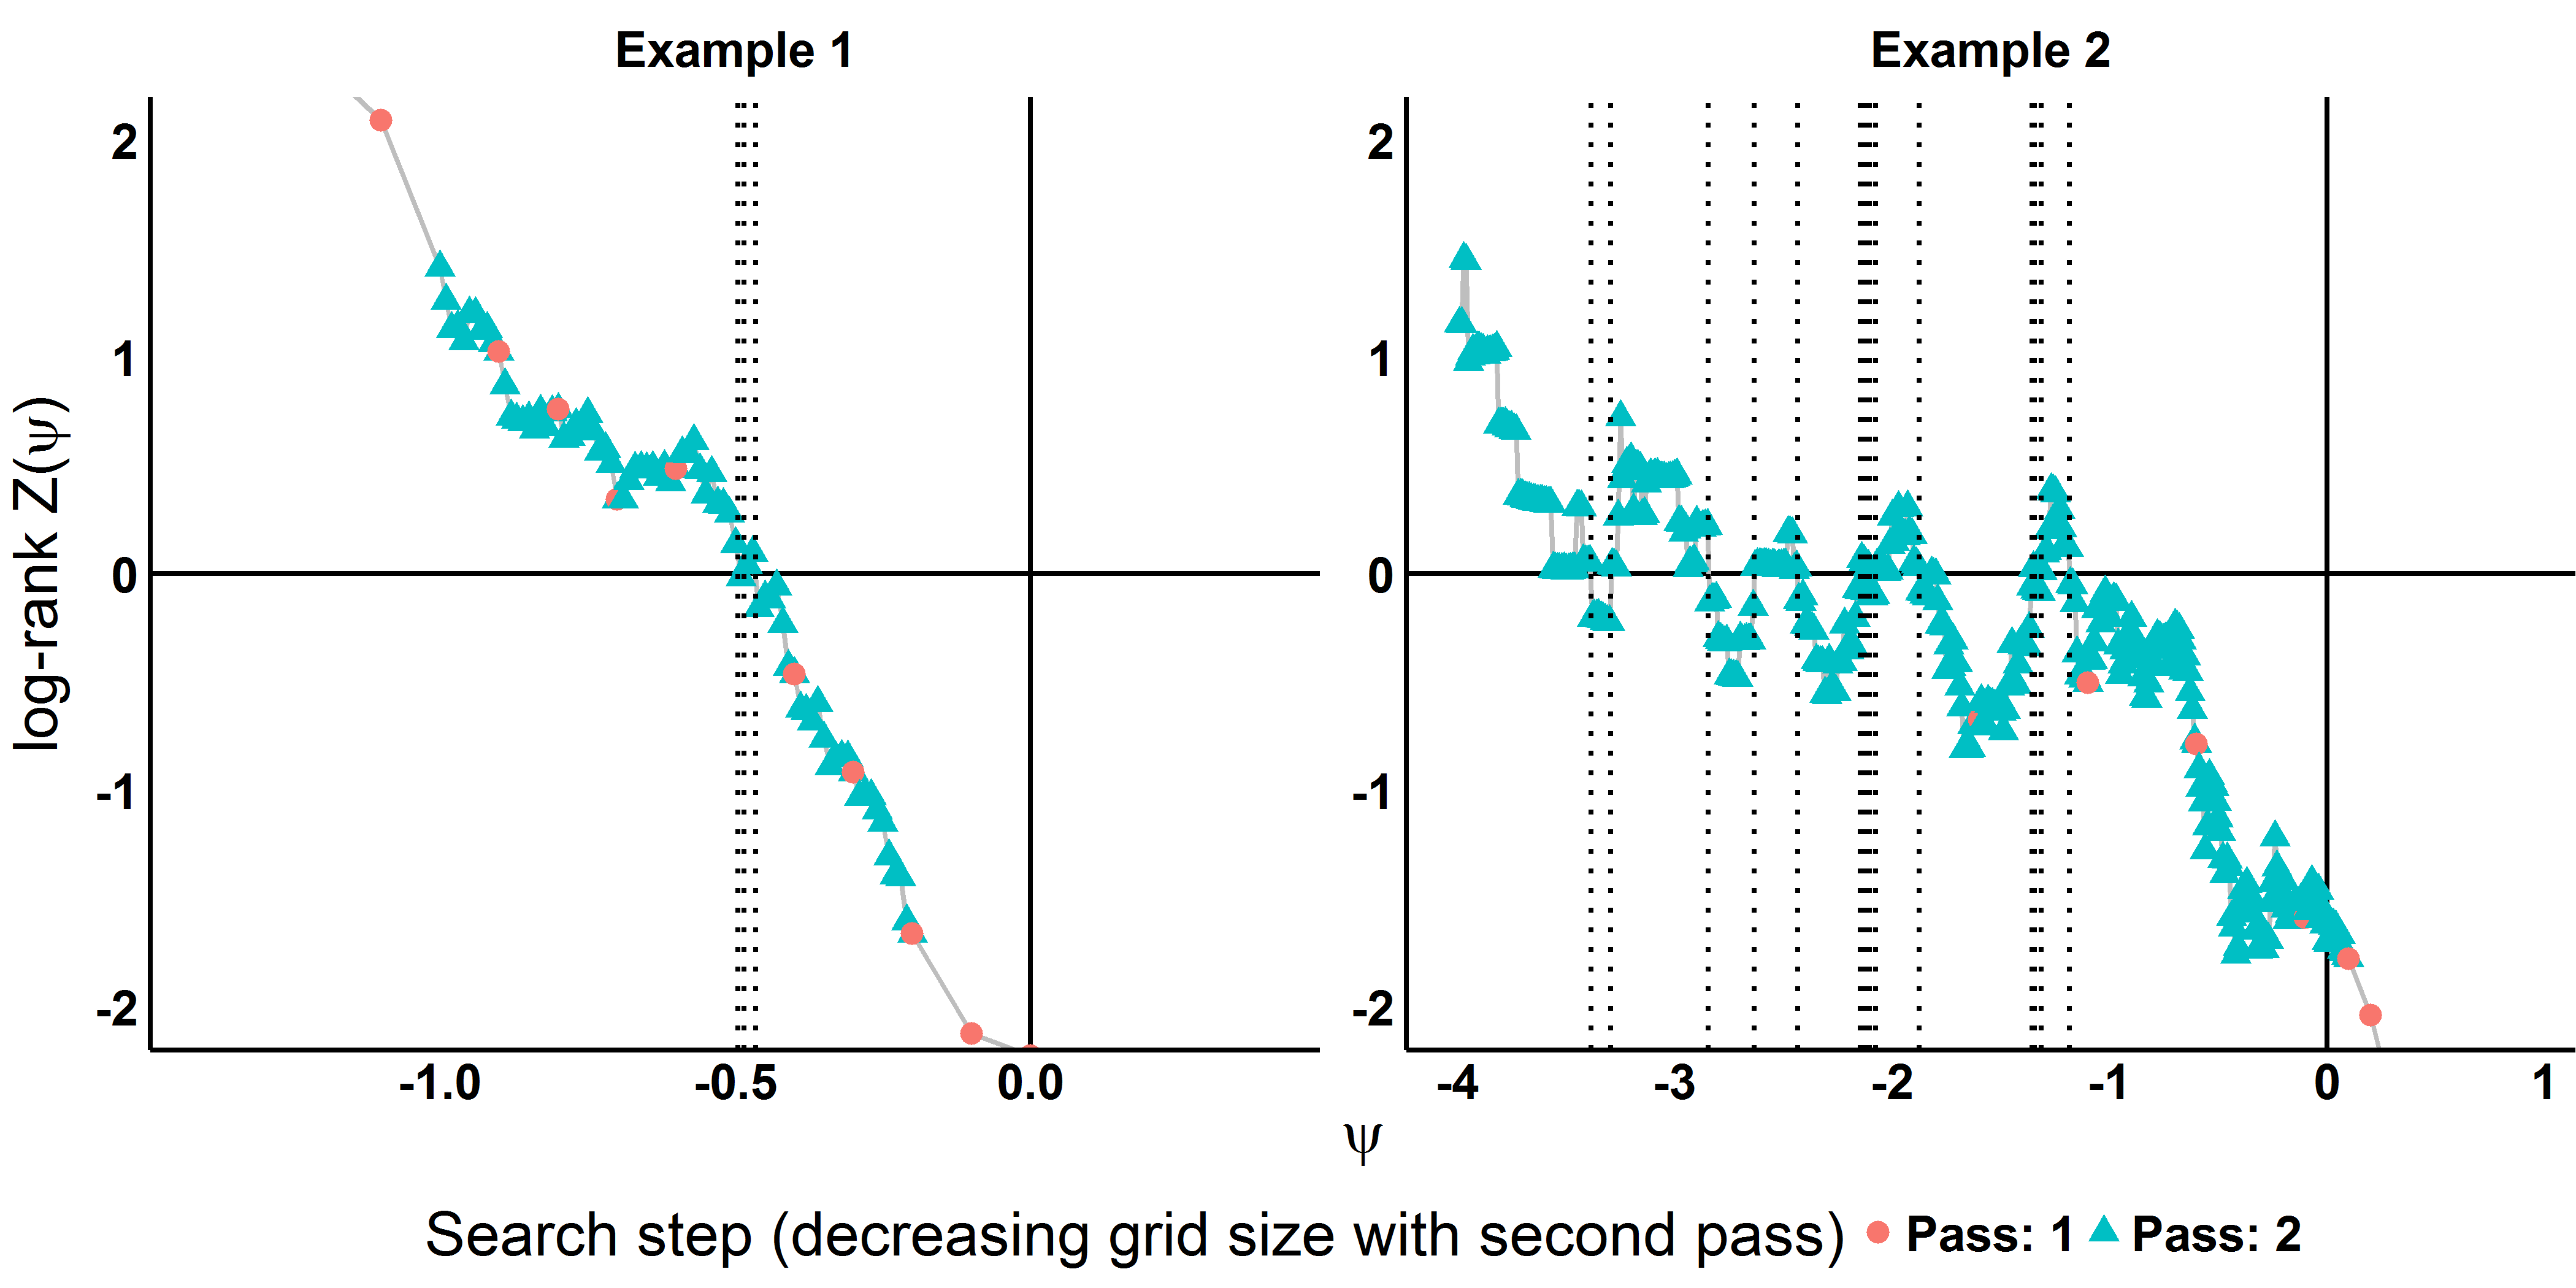
\includegraphics[width=13cm]{images/chap_sim3/badsearch.png}
\caption{\label{F:chap_sim3:badgest} Two examples of problems in g-estimation using log-rank test statistic. In Example 1 the potential values for $\hat{\psi}$ are all quite similar ranging from  $-0.495$ to $-0.465$ while for Example 2 the values where $z(\psi)=0$ range from $-3.385$ to $-1.185$. } 
\end{figure}

\begin{figure}[ht]
\centering
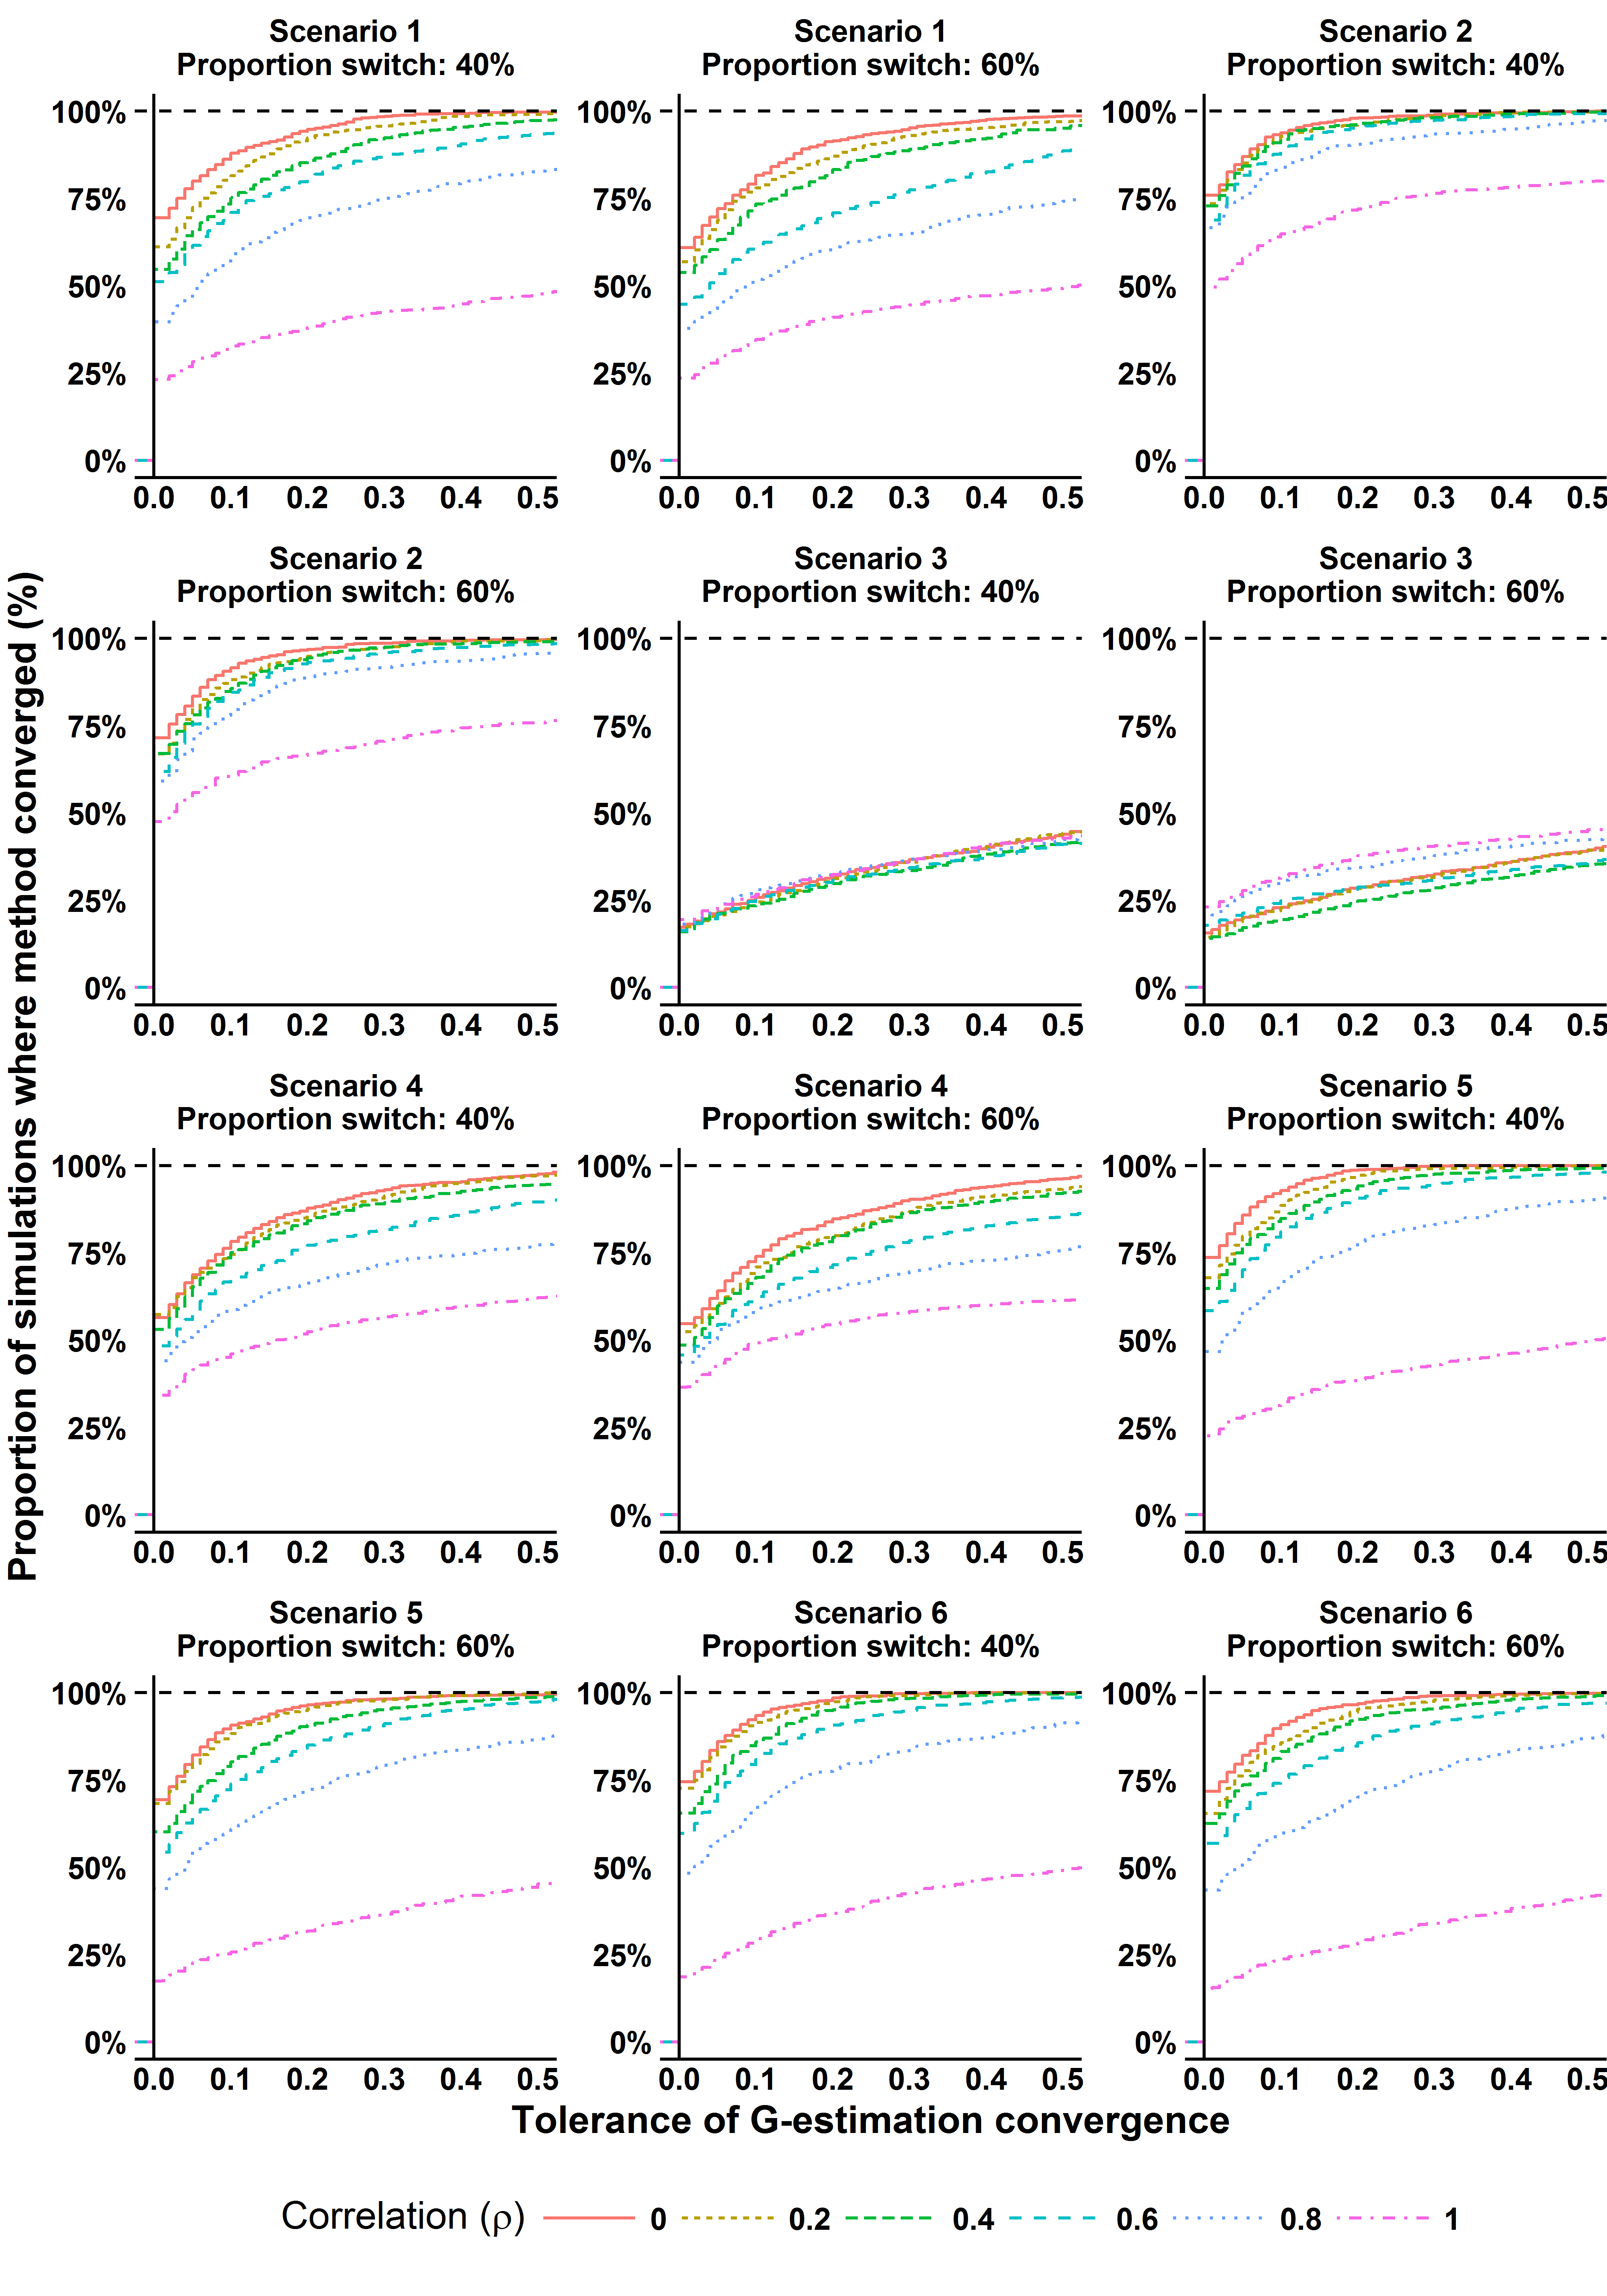
\includegraphics[width=13cm]{images/chap_sim3/conv_cdf.png}
\caption{\label{F:chap_sim3:convcdf}  This figure shows the cumulative distribution of proportion of simulations where the ``on treatment'' approach to rank-preserving failure time (RPSFT) converged for different tolerances on convergence. A tolerance of 0 implies a unique solution was found with increasing tolerance allowing a broader range of multiple solutions for $\psi$ still being considered as converged. Based on this it was decided to investigate further a tolerance of 0.2 in the estimates of $\psi$. Even with this imputation the convergence in Scenario 3 is very poor.} 
\end{figure}

\clearpage

\section{Results}

Table \ref{T:chap_sim3:simres} shows a summary of the results for selected methods grouped by scenario while complete results can be found in Appendix \ref{A:sim3res}. The same methods as discussed in Section \ref{S:chap_sim2:resmeth} are used to assess the methods with the outcome of interest again a hazard ratio for experimental treatment compared to control for overall survival. As with the previous simulation study the results for the RPSFT method using both wilcoxon and log-rank tests in the g-estimation were very similar so only the results using the log-rank test are discussed here.

\begin{table}[ht] 
\caption{The range of bias, MSE, coverage and convergence across scenarios for selected methods\label{T:chap_sim3:simres}}
\centering 
\scalebox{0.9}{
% latex table generated in R 3.3.1 by xtable 1.8-2 package
% Thu Sep 15 18:21:03 2016
\scalebox{0.9}{
\begin{tabular}{lrrrrr}
  \hline
\hline
Scenarios & Method & Bias  & MSE & Coverage & Convergence  \\  &  & $(\%)$ &   & $(\%)$ & $(\%)$ \\  &  & min, max & min, max & min, max & min, max \\ 
  \hline
1 and 2 & ITT &   5.42, 25.54 & 0.02, 0.04 & 66.5, 94.2 & 100.0, 100.0 \\ 
  1 and 2 & PP-CENS &  -1.97, 47.03 & 0.01, 0.23 & 44.0, 95.4 & 100.0, 100.0 \\ 
  1 and 2 & TVC &  -3.02, 75.03 & 0.01, 0.51 &  5.9, 94.9 & 100.0, 100.0 \\ 
  1 and 2 & TVC2 &  -1.89, 56.00 & 0.01, 0.31 & 31.2, 95.4 & 100.0, 100.0 \\ 
  1 and 2 & RPSFT-TG-LR &  -1.09,  8.25 & 0.02, 0.06 & 90.1, 96.1 & 90.6, 99.7 \\ 
  1 and 2 & RPSFT-OT-LR-TU-TOL &  -2.35, 21.12 & 0.03, 0.07 & 74.1, 94.0 & 40.7, 97.9 \\ 
  1 and 2 & RPSFT-OT-LR-V-TOL &  -3.14, 21.11 & 0.03, 0.16 & 85.9, 95.0 & 40.7, 97.9 \\ 
  1 and 2 & 2SAFT &  -3.14,  2.34 & 0.01, 0.03 & 84.5, 95.6 & 100.0, 100.0 \\ 
  1 and 2 & MIPE-ALL & -22.91, -2.60 & 0.05, 0.07 & 43.4, 69.8 & 100.0, 100.0 \\ 
  1 and 2 & MIPE-WEIB &   4.04, 26.12 & 0.03, 0.10 &  & 25.7, 55.4 \\ 
   \hline
3 and 4 & ITT &  11.92, 44.11 & 0.02, 0.07 & 36.2, 86.8 & 100.0, 100.0 \\ 
  3 and 4 & PP-CENS & -10.56, 46.02 & 0.01, 0.18 & 46.6, 96.2 & 100.0, 100.0 \\ 
  3 and 4 & TVC & -14.97, 69.01 & 0.01, 0.35 & 11.1, 96.0 & 100.0, 100.0 \\ 
  3 and 4 & TVC2 & -10.87, 53.93 & 0.01, 0.23 & 33.9, 96.0 & 100.0, 100.0 \\ 
  3 and 4 & RPSFT-TG-LR & -22.72, 17.08 & 0.03, 0.07 & 83.0, 92.9 & 93.5, 99.9 \\ 
  3 and 4 & RPSFT-OT-LR-TU-TOL & -12.72, 35.50 & 0.04, 0.10 & 57.2, 86.3 & 33.4, 87.4 \\ 
  3 and 4 & RPSFT-OT-LR-V-TOL & -13.92, 41.12 & 0.04, 0.20 & 61.8, 89.5 & 33.4, 87.4 \\ 
  3 and 4 & 2SAFT & -24.66,  1.19 & 0.01, 0.03 & 61.6, 95.0 & 100.0, 100.0 \\ 
  3 and 4 & MIPE-ALL & -51.25,  7.60 & 0.05, 0.08 & 14.5, 59.9 & 100.0, 100.0 \\ 
  3 and 4 & MIPE-WEIB & -11.07, 41.90 & 0.02, 0.15 &  & 21.8, 48.8 \\ 
   \hline
5 and 6 & ITT &   3.75,  13.75 & 0.01, 0.02 & 85.5, 95.8 & 100.0, 100.0 \\ 
  5 and 6 & PP-CENS &   0.52,  48.23 & 0.01, 0.15 & 44.6, 95.6 & 100.0, 100.0 \\ 
  5 and 6 & TVC &   4.99,  95.90 & 0.01, 0.50 &  1.7, 95.1 & 100.0, 100.0 \\ 
  5 and 6 & TVC2 &   0.52,  59.28 & 0.01, 0.21 & 26.7, 95.5 & 100.0, 100.0 \\ 
  5 and 6 & RPSFT-TG-LR & -15.61,  -2.60 & 0.02, 0.03 & 87.5, 93.2 & 98.4, 100.0 \\ 
  5 and 6 & RPSFT-OT-LR-TU-TOL & -11.28,   5.77 & 0.02, 0.04 & 80.6, 90.7 & 36.7, 98.6 \\ 
  5 and 6 & RPSFT-OT-LR-V-TOL & -13.97,   3.04 & 0.02, 0.05 & 84.8, 92.9 & 36.7, 98.6 \\ 
  5 and 6 & 2SAFT &  -0.04,   2.62 & 0.01, 0.02 & 86.1, 94.9 & 100.0, 100.0 \\ 
  5 and 6 & MIPE-ALL & -35.27, -21.33 & 0.06, 0.09 & 27.2, 43.9 & 100.0, 100.0 \\ 
  5 and 6 & MIPE-WEIB & -13.93,   4.87 & 0.02, 0.05 &  & 25.1, 31.1 \\ 
   \hline
\end{tabular}
}

}
\end{table}

\clearpage

\subsection{Convergence}

As already discussed in Section \ref{S:chap_sim3:gest} the convergence for the ``on treatment'' approach to RPSFT was poor in this simulation study which can be seen in Figure \ref{F:chap_sim3:conv}. In particular the convergence is lower for higher correlations between time to progression and overall survival. Of interest here is that the ``treatment group'' approach to RPSFT again appears to have no convergence issues and converges to a unique solution much more consistently than the iterative parameter estimation procedure (MIPE). Again as the primary benefit of the iterative parameter estimation method is an improved estimation procedure in exchange for making a parametric assumption on the survival time distribution this is unexpected. Finally the simple methods and the two-stage AFT (2SAFT) converge consistently across all the scenarios investigated. 

\begin{figure}[ht]
\centering
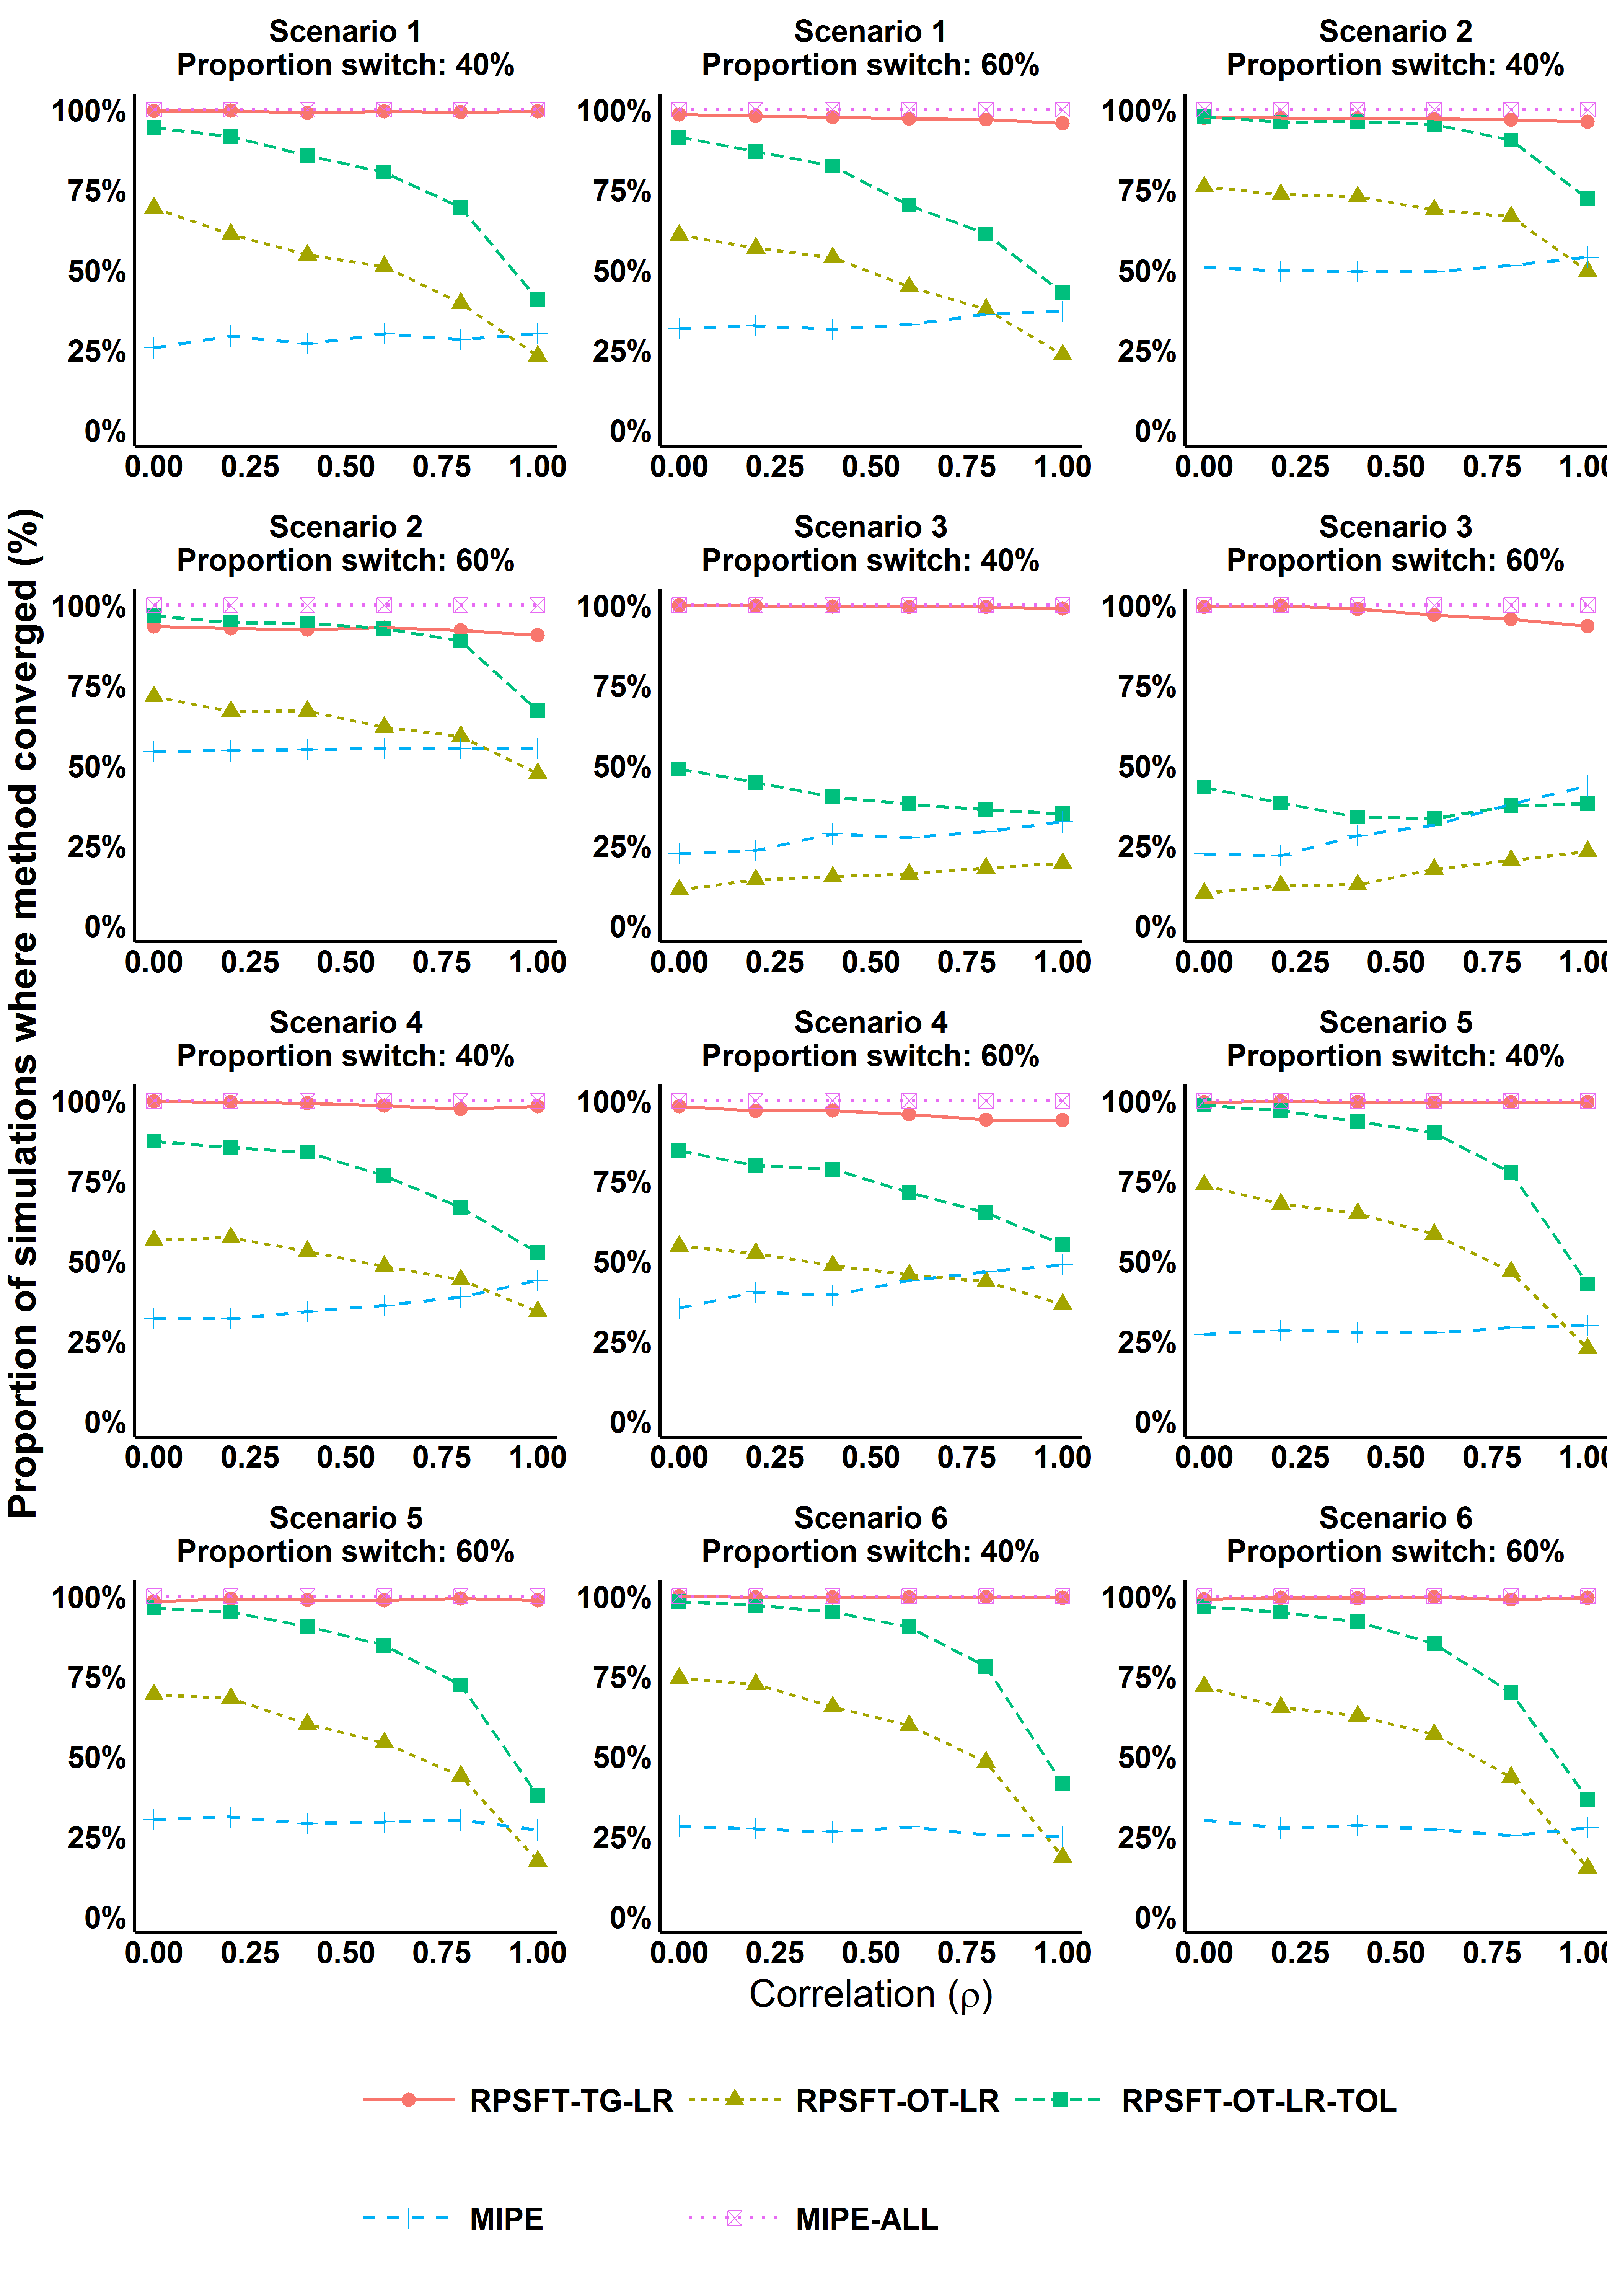
\includegraphics[width=13cm]{images/chap_sim3/comp_conv.png}
\caption{\label{F:chap_sim3:conv}  This figure shows the proportion of simulations where the complex methods rank-preserving structural failure time (RPSFT) and modified iterative parameter estimation (MIPE) converged to a unique solution. For RPSFT while convergence was acceptable in the ``treatment group'' approach (RPSFT-TG) for the ``on treatment'' approach (RPSFT-OT) the convergence was poor in the majority of scenarios particularly where correlation was high with the imputation approach only having limited improvement (RPSFT-OT-TOL) in these cases. The iterative parameter estimation (MIPE) approach performs much worse than the ``treatment group'' approach to RPSFT whose assumptions it shares and is also poor compared to the ``on treatment'' approach to RPSFT for the majority of scenarios. } 
\end{figure}

\clearpage


\subsection{Bias}

\subsubsection{Simple methods}

Figure \ref{F:chap_sim3:simple_bias} shows the bias for all the simple methods. The same patterns to the bias as seen in the previous simulation study are again apparent. For the per-protocol analysis excluding switch patients (PP-EX) there is again a large bias to overestimate the treatment effect regardless of correlation unless the time to progression is correlated perfectly with overall survival which is an implausible scenario. 

In the previous simulation study the Per-protocol Censoring at Switch (PP-CENS) analysis and the analysis including Treatment as a time-varying covariate (TVC and TVC2) were unbiased only when there was no correlation between time to progression and overall survival. In the scenarios investigated here this is again the case. It can be seen that the bias increases with increasing correlation between time to progression and overall survival. 

Across all the scenarios the ITT analysis underestimated the true treatment effect as expected. As seen previously the amount of bias is dependent on the magnitude of switch treatment effect so for scenarios 2 and 6 where the effect of switch treatment is minimal the ITT analysis shows less bias. This also explains to a certain extent the trend to decreasing bias with increasing correlation seen in scenario 3 as for this scenario the true treatment effect is also reduced with increasing correlation.

\begin{figure}[ht]
\centering
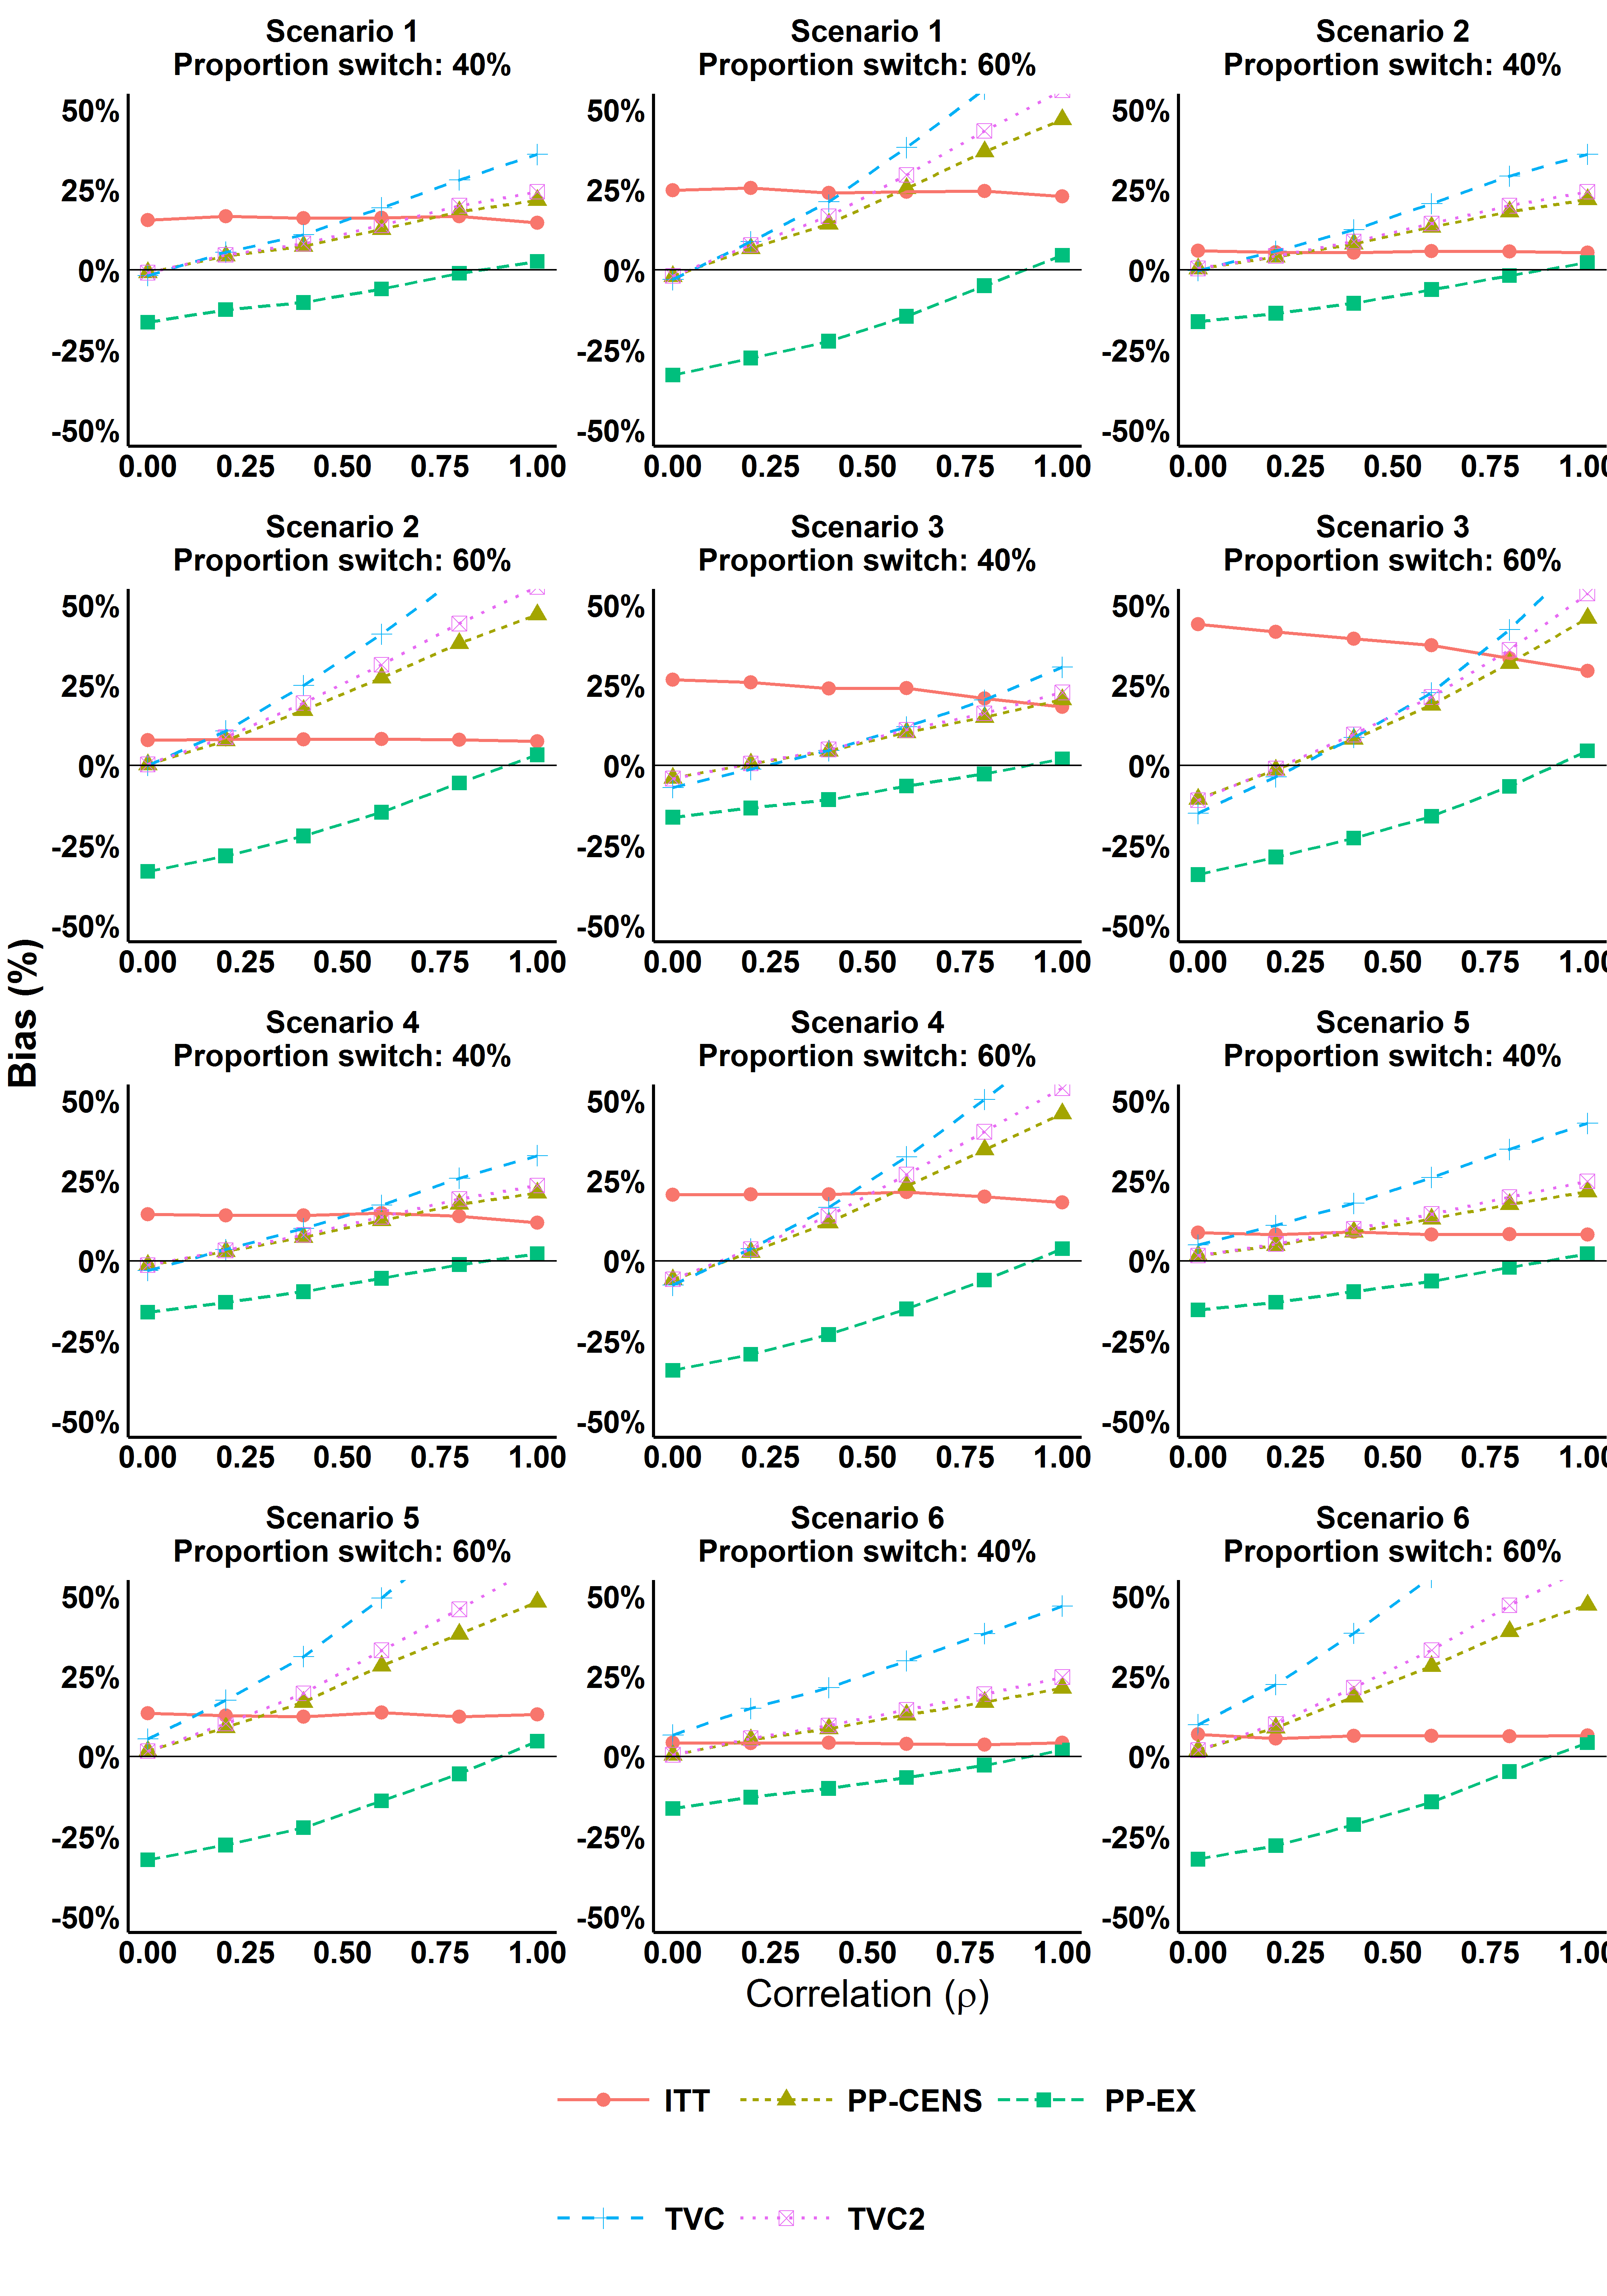
\includegraphics[width=13cm]{images/chap_sim3/simple_bias.png}
\caption{\label{F:chap_sim3:simple_bias} The bias for each of the simple methods in the scenarios for simulation study 2. For the Per-protocol Excluding Switch Patients (PP-EX) analysis the bias is large across all correlations. As with simulation study 1 for the Per-protocol Censoring at Switch (PP-CENS) analysis and the analysis including Treatment as a time-varying covariate (TVC and TVC2) there is reduced bias when there is no correlation between survival and time to progression but a very large bias otherwise. The ITT analysis consistently underestimates the true treatment effect across all scenarios mostly independently of correlation.} 
\end{figure}

\clearpage

\subsubsection{Complex methods}

Figure \ref{F:chap_sim3:comp_bias12} show the percentage bias for selected complex methods investigated in scenario 1 and 2. Compared to the simple methods the percentage bias is much reduced with the ``treatment group'' approach to RPSFT and two-stage AFT (2SAFT) performing the best. It is unclear why the iterative parameter estimation approach (MIPE) overestimates the treatment effect while the weibull model approach (MIPE-WEIB) simultaneously underestimates the treatment effect but performance is noticeably worse than the RPSFT approaches. 


For scenarios 3 and 4 the percentage bias is shown in Figure \ref{F:chap_sim3:comp_bias34} and the data generating mechanism could be expected to match closer to the assumptions of the ``on treatment'' approach to RPSFT with the treatment effect only applying during exposure to experimental treatment. Despite this the bias of this method and the bias of the ``treatment group'' approach are very similar with the ``treatment group'' approach having slightly lower bias for large correlations. In these scenarios there again seems to be limited benefit to using the IPE method compared to the RPSFT method with both approaches to estimating a hazard ratio using the MIPE approach having a greater range of bias compared to the RPSFT approaches. In these scenarios the two-stage AFT method performs relatively badly compared to the good performance elsewhere. To investigate this further Figure \ref{F:chap_sim3:2saft_bias34} shows the bias for the different implementations considered and it can be seen that for scenario 3 the bias can be improved by avoiding re-censoring (2SAFT-NC), however, this doesn't seem to be a universal fix as this increases the bias for scenario 4.

For scenarios 5 and 6 the bias of the RPSFT and MIPE methods is expected to be larger due to the violation of the common treatment effect assumption and as seen in Figure \ref{F:chap_sim3:comp_bias56} these methods do tend to overestimate the treatment effect here independently of correlation. Meanwhile the bias for the two-stage AFT method is very low across all these scenarios regardless of correlation with a maximum bias of 2.6\%.


\begin{figure}[ht]
\centering
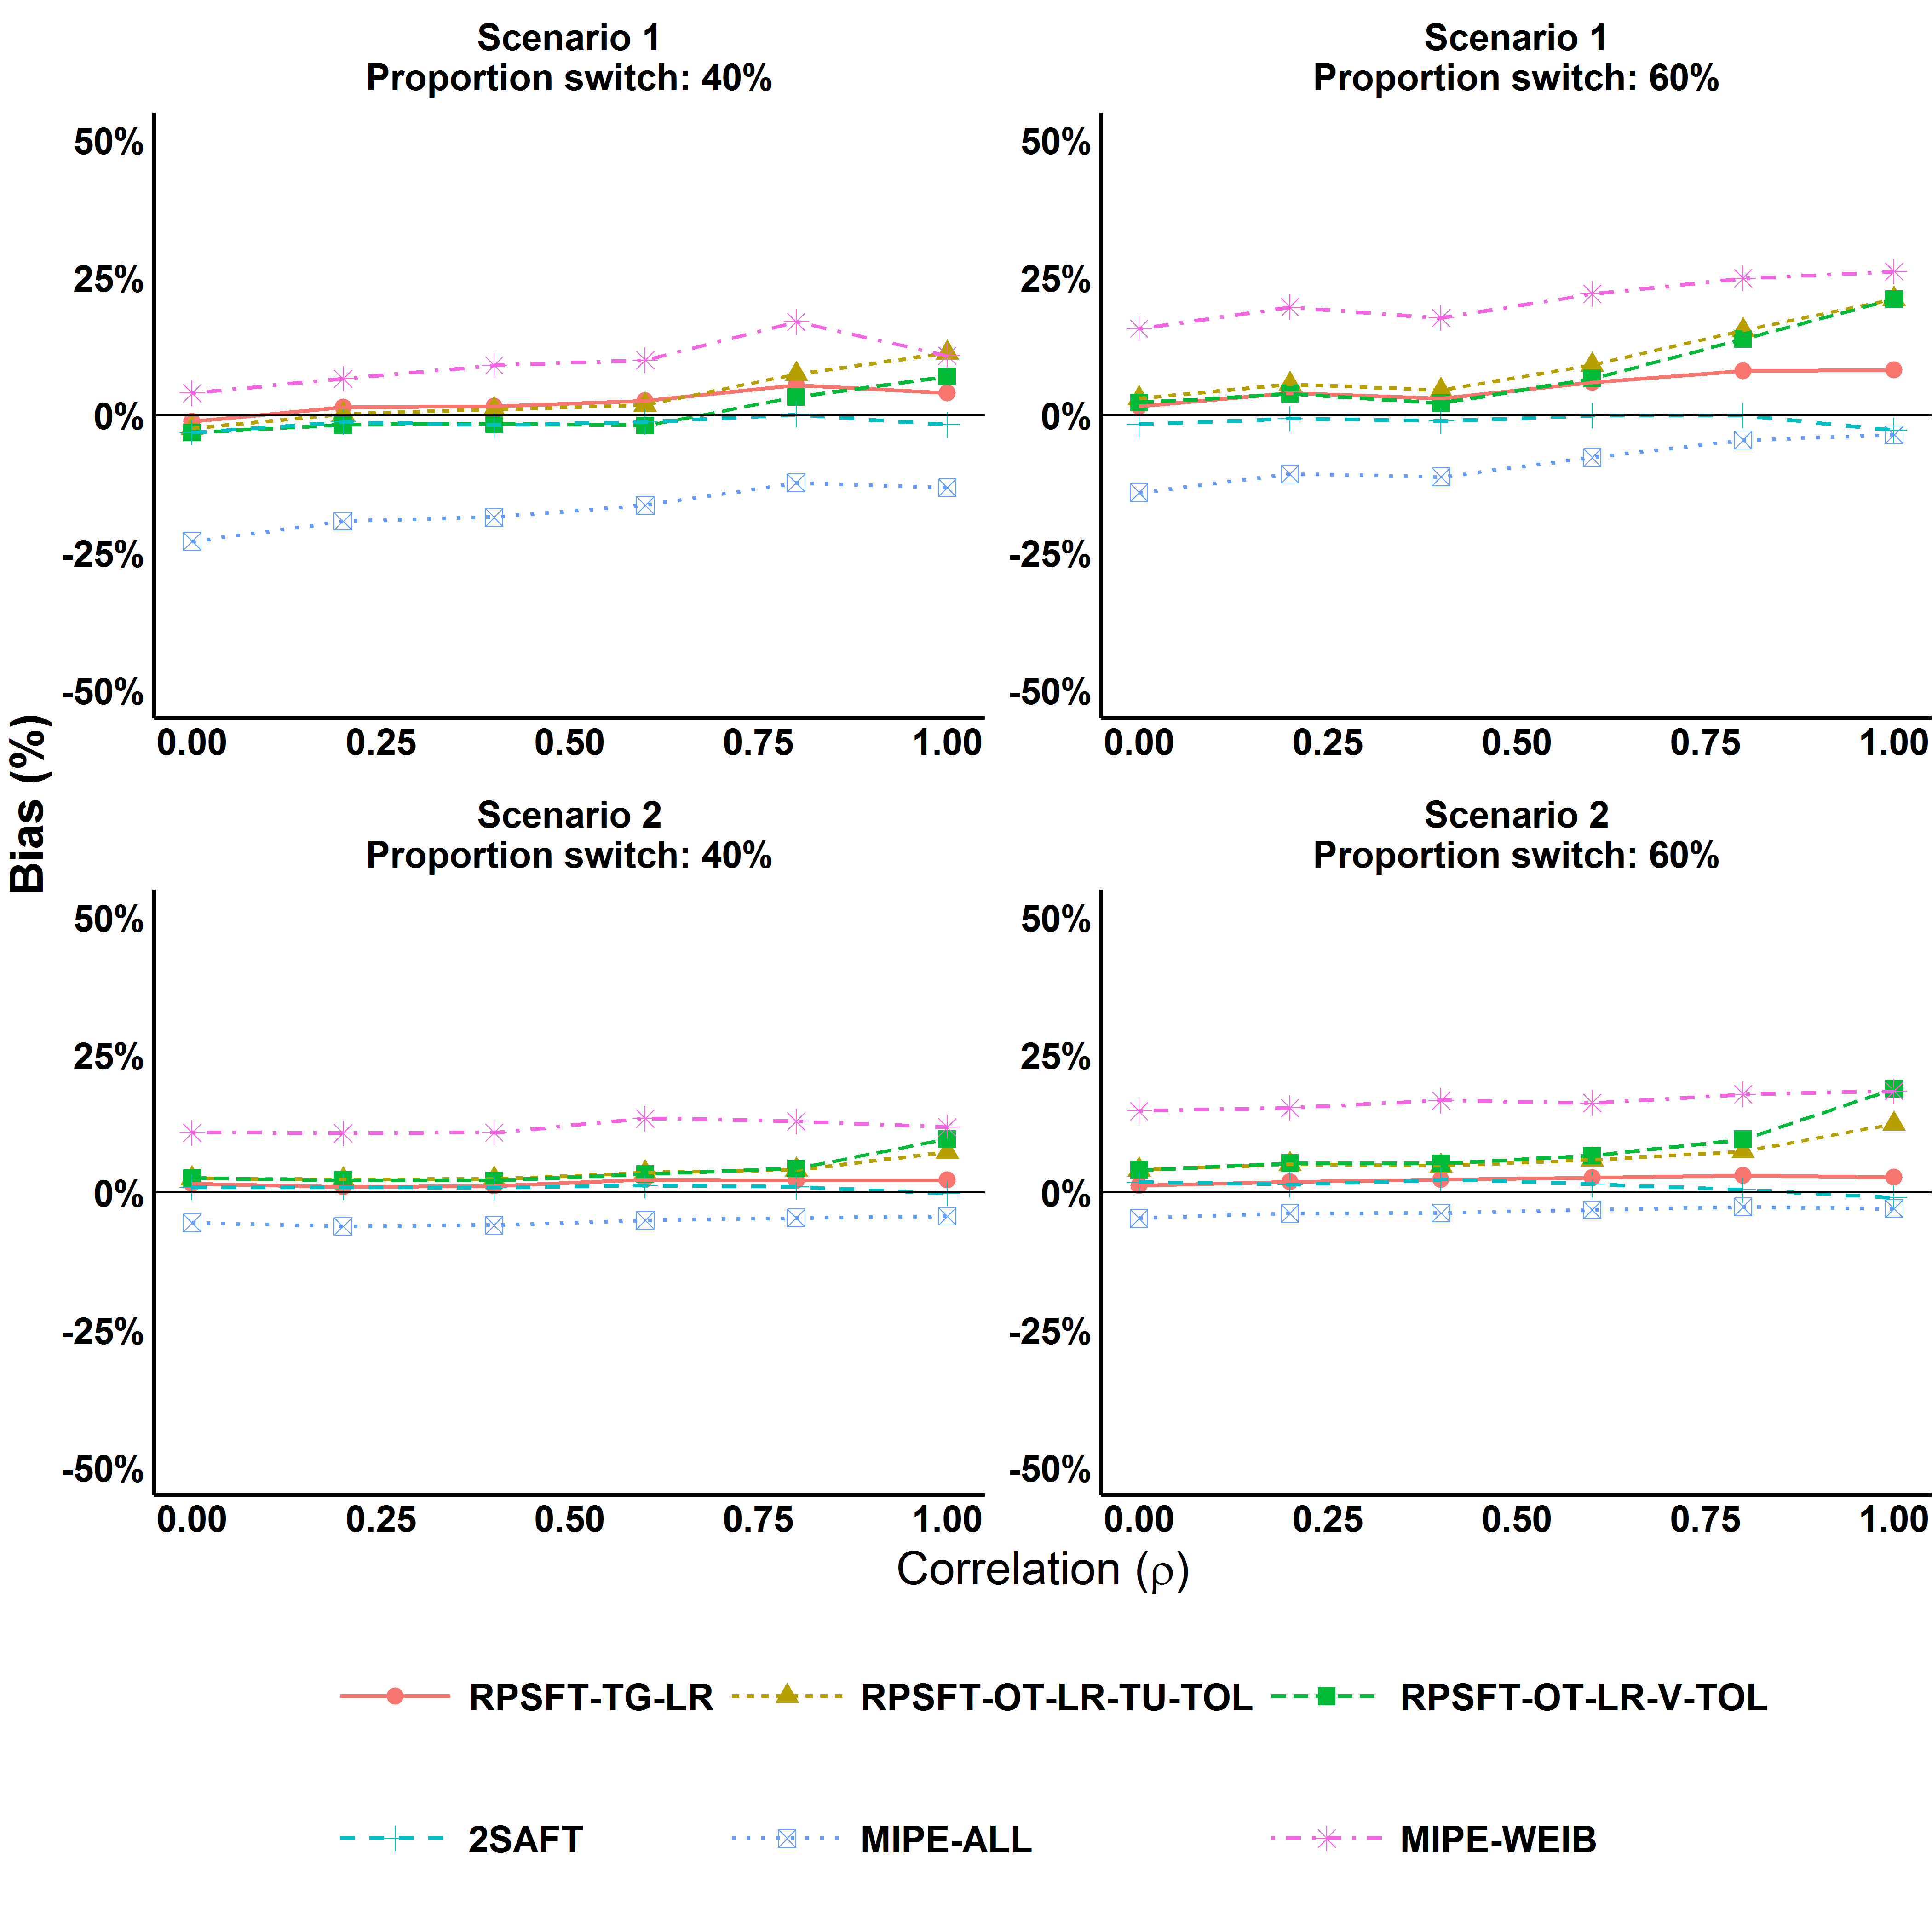
\includegraphics[width=13cm]{images/chap_sim3/comp_bias12.png}
\caption{\label{F:chap_sim3:comp_bias12} The bias for selected implementations of the complex methods for Scenario 1 and 2. In these scenarios there is a reduction in hazard during treatment and a reduced residual effect after treatment. For Scenario 1 the ``true''  hazard ratio is around 0.7 while for Scenario 2 it is approximately 0.9 as shown in Figure \ref{F:chap_sim3:truehr} which explains the lower bias seen in Scenario 2 compared to Scenario 1. In general the different approaches to RPSFT used here have a similar level of bias with the ``treatment group'' approach (RPSFT-TG) generally performing better though the increased bias for the ``on treatment'' approach (RPSFT-OT) seen with high correlations maybe partially due to the low convergence of this method in scenarios with $\rho \geq 0.8$. The two-stage AFT (2SAFT) including recensoring and progression free survival as a covariate has very low bias in these scenarios.}
\end{figure}

\begin{figure}[ht]
\centering
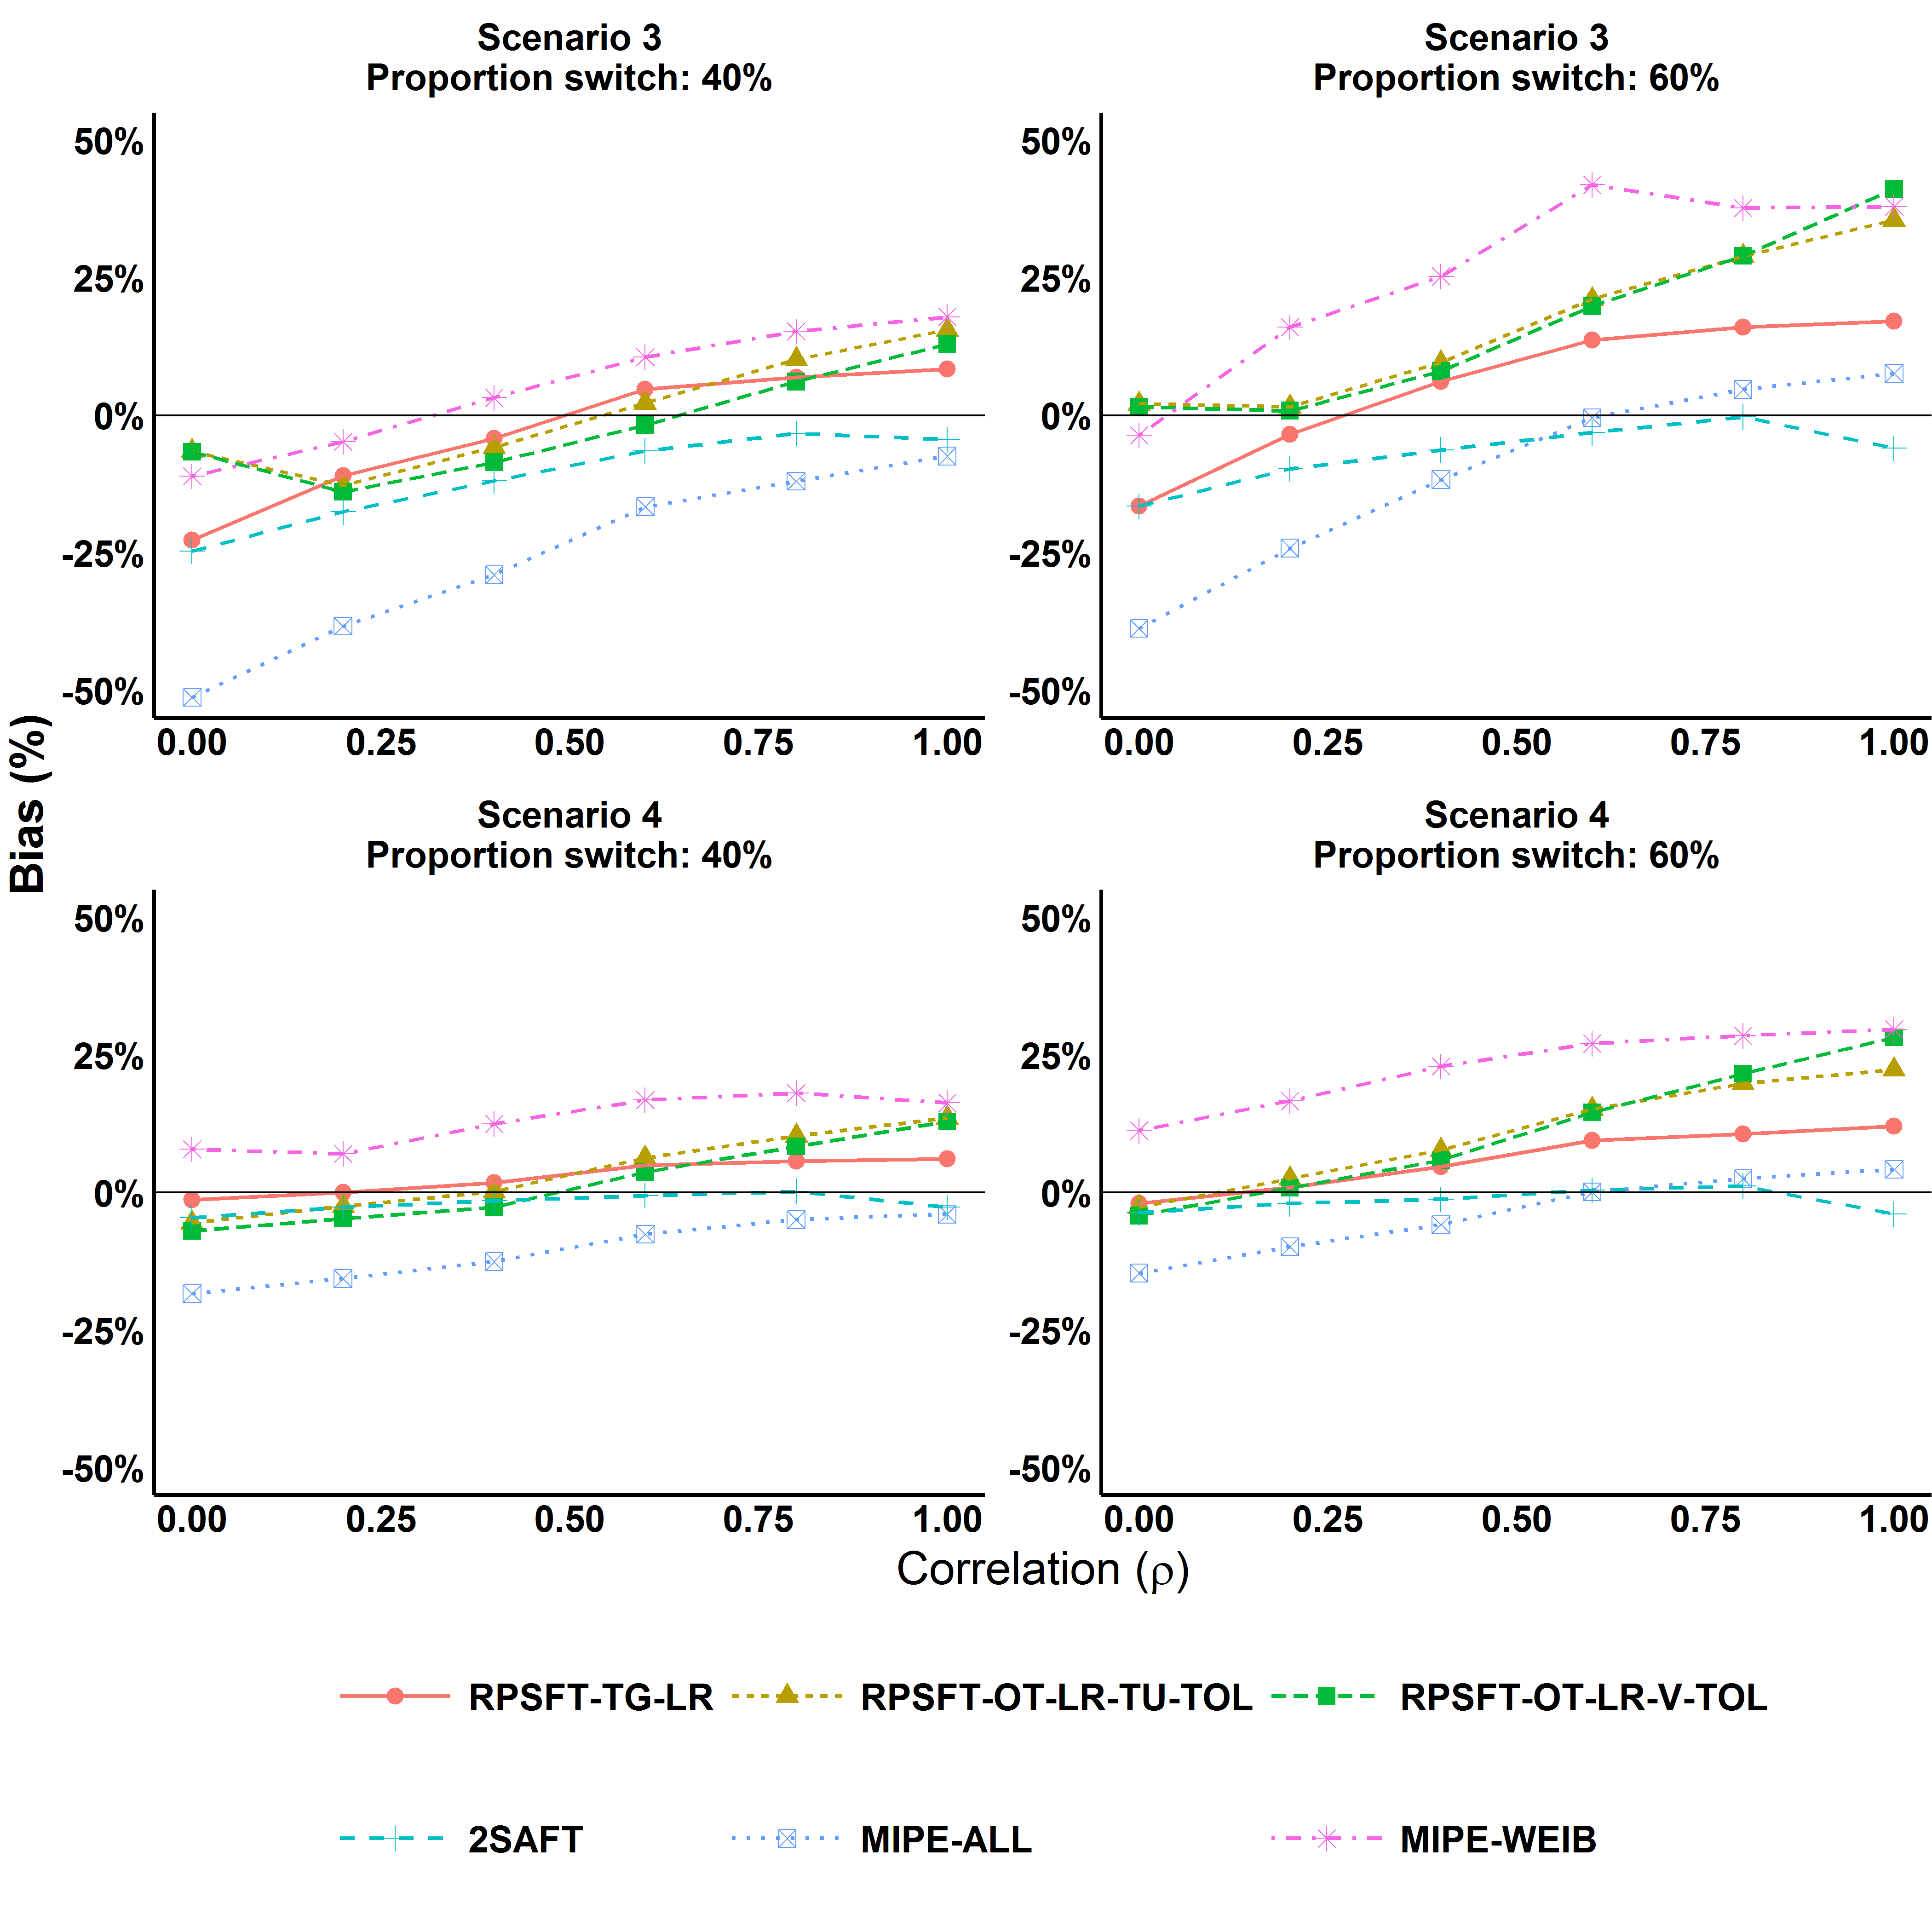
\includegraphics[width=12cm]{images/chap_sim3/comp_bias34.png}
\caption{\label{F:chap_sim3:comp_bias34} The bias for selected implementations of the complex methods for Scenario 3 and 4. In these scenarios the treatment is simulated to only reduce the risk of death during treatment. For the ``on treatment'' approach to RPSFT (RPSFT-OT-TOL) and the modified iterative parameter estimation using the weibull model (MIPE-WEIB) it should be noted that convergence is very low for Scenario 3. It was expected that the ``on treatment'' approach to RPSFT would perform better here as it is closer to the data generating mechanism, however, this does not appear to be the case with only a slight reduction in bias compared to the ``treatment group'' approach. Surprisingly the two-stage AFT (2SAFT) including recensoring and progression free survival as a covariate performs badly here with a few scenarios having greater bias than the RPSFT or MIPE methods. While it appears that there is some relationship between correlation and bias here this is somewhat hard to interpret as the ``true'' hazard ratio for these scenarios is also strongly related to correlation as shown in Figure \ref{F:chap_sim3:truehr}.} 
\end{figure}


\begin{figure}[ht]
\centering
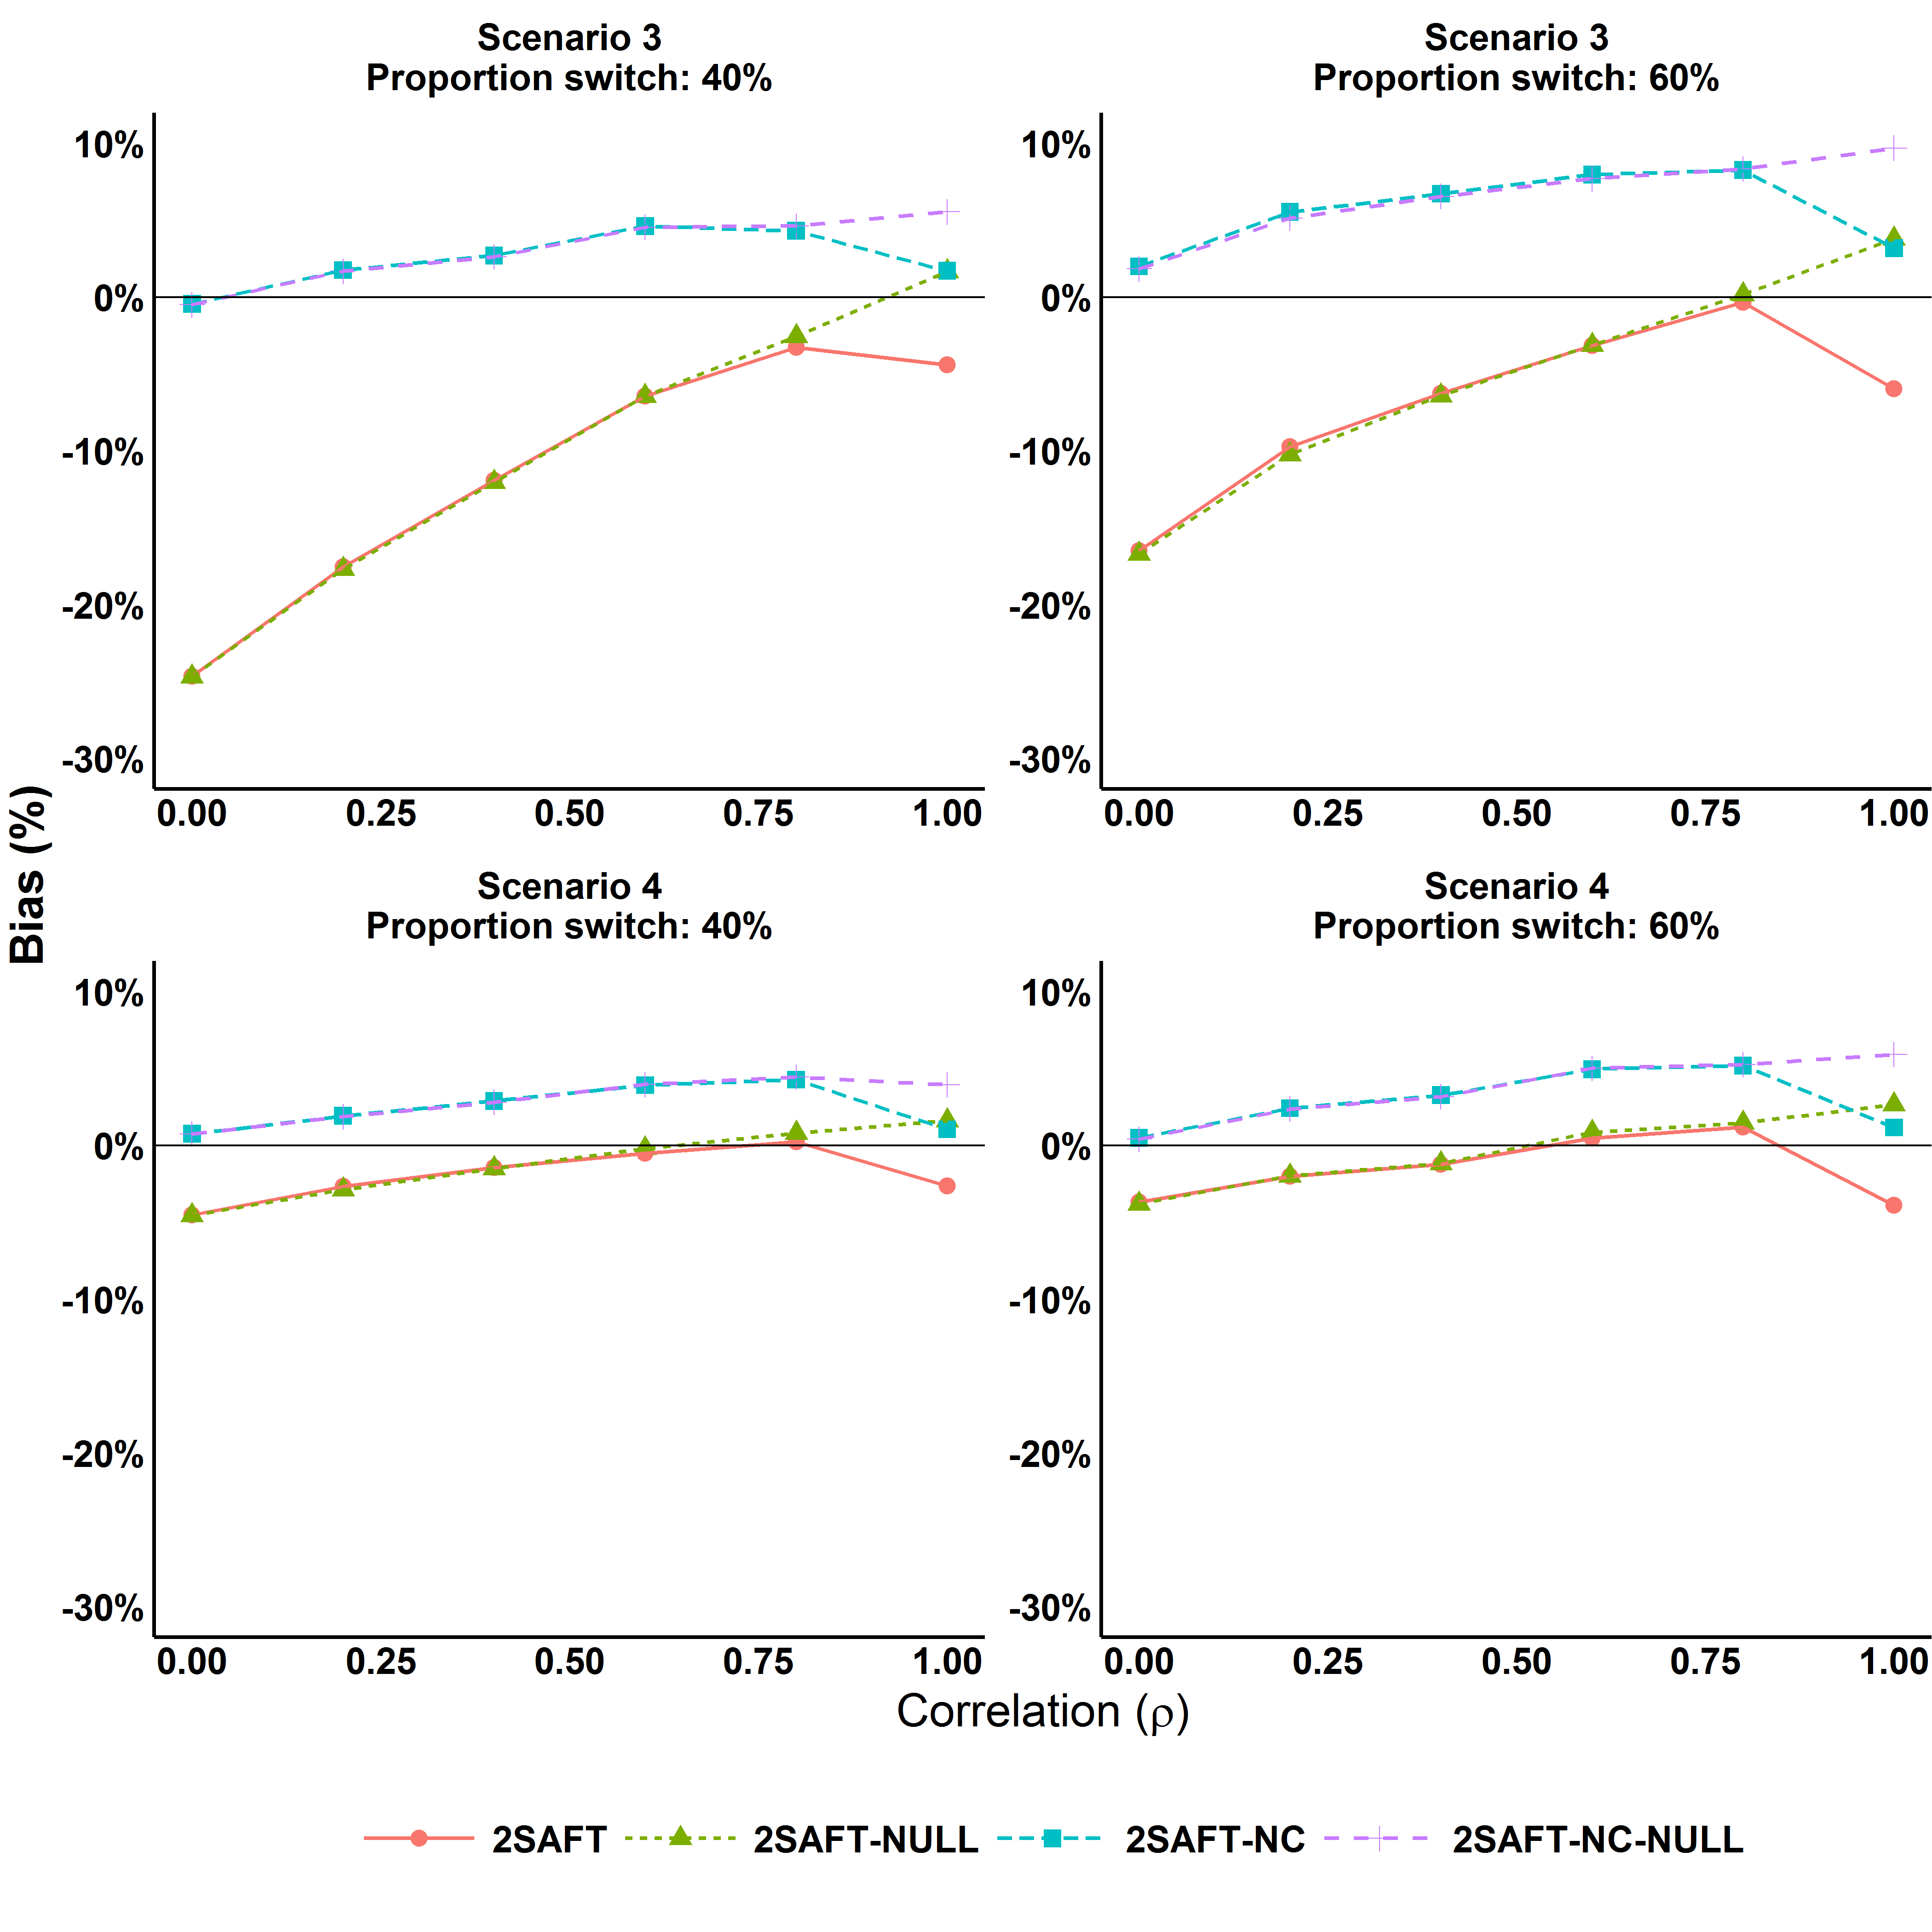
\includegraphics[width=12cm]{images/chap_sim3/2saft_bias.png}
\caption{\label{F:chap_sim3:2saft_bias34} The bias for all implementations of two-stage AFT model investigated for Scenario 3 and 4. In these scenarios the treatment is simulated to only reduce the risk of death during treatment. For scenario 3 it can be seen that the inclusion of a covariate for PFS into the model (2SAFT) or not (2SAFT-NULL) has negligible impact on the bias for the method compared to the reduction in bias when no-recensoring is performed (2SAFT-NC) and (2SAFT-NC-NULL).} 
\end{figure}


\begin{figure}[ht]
\centering
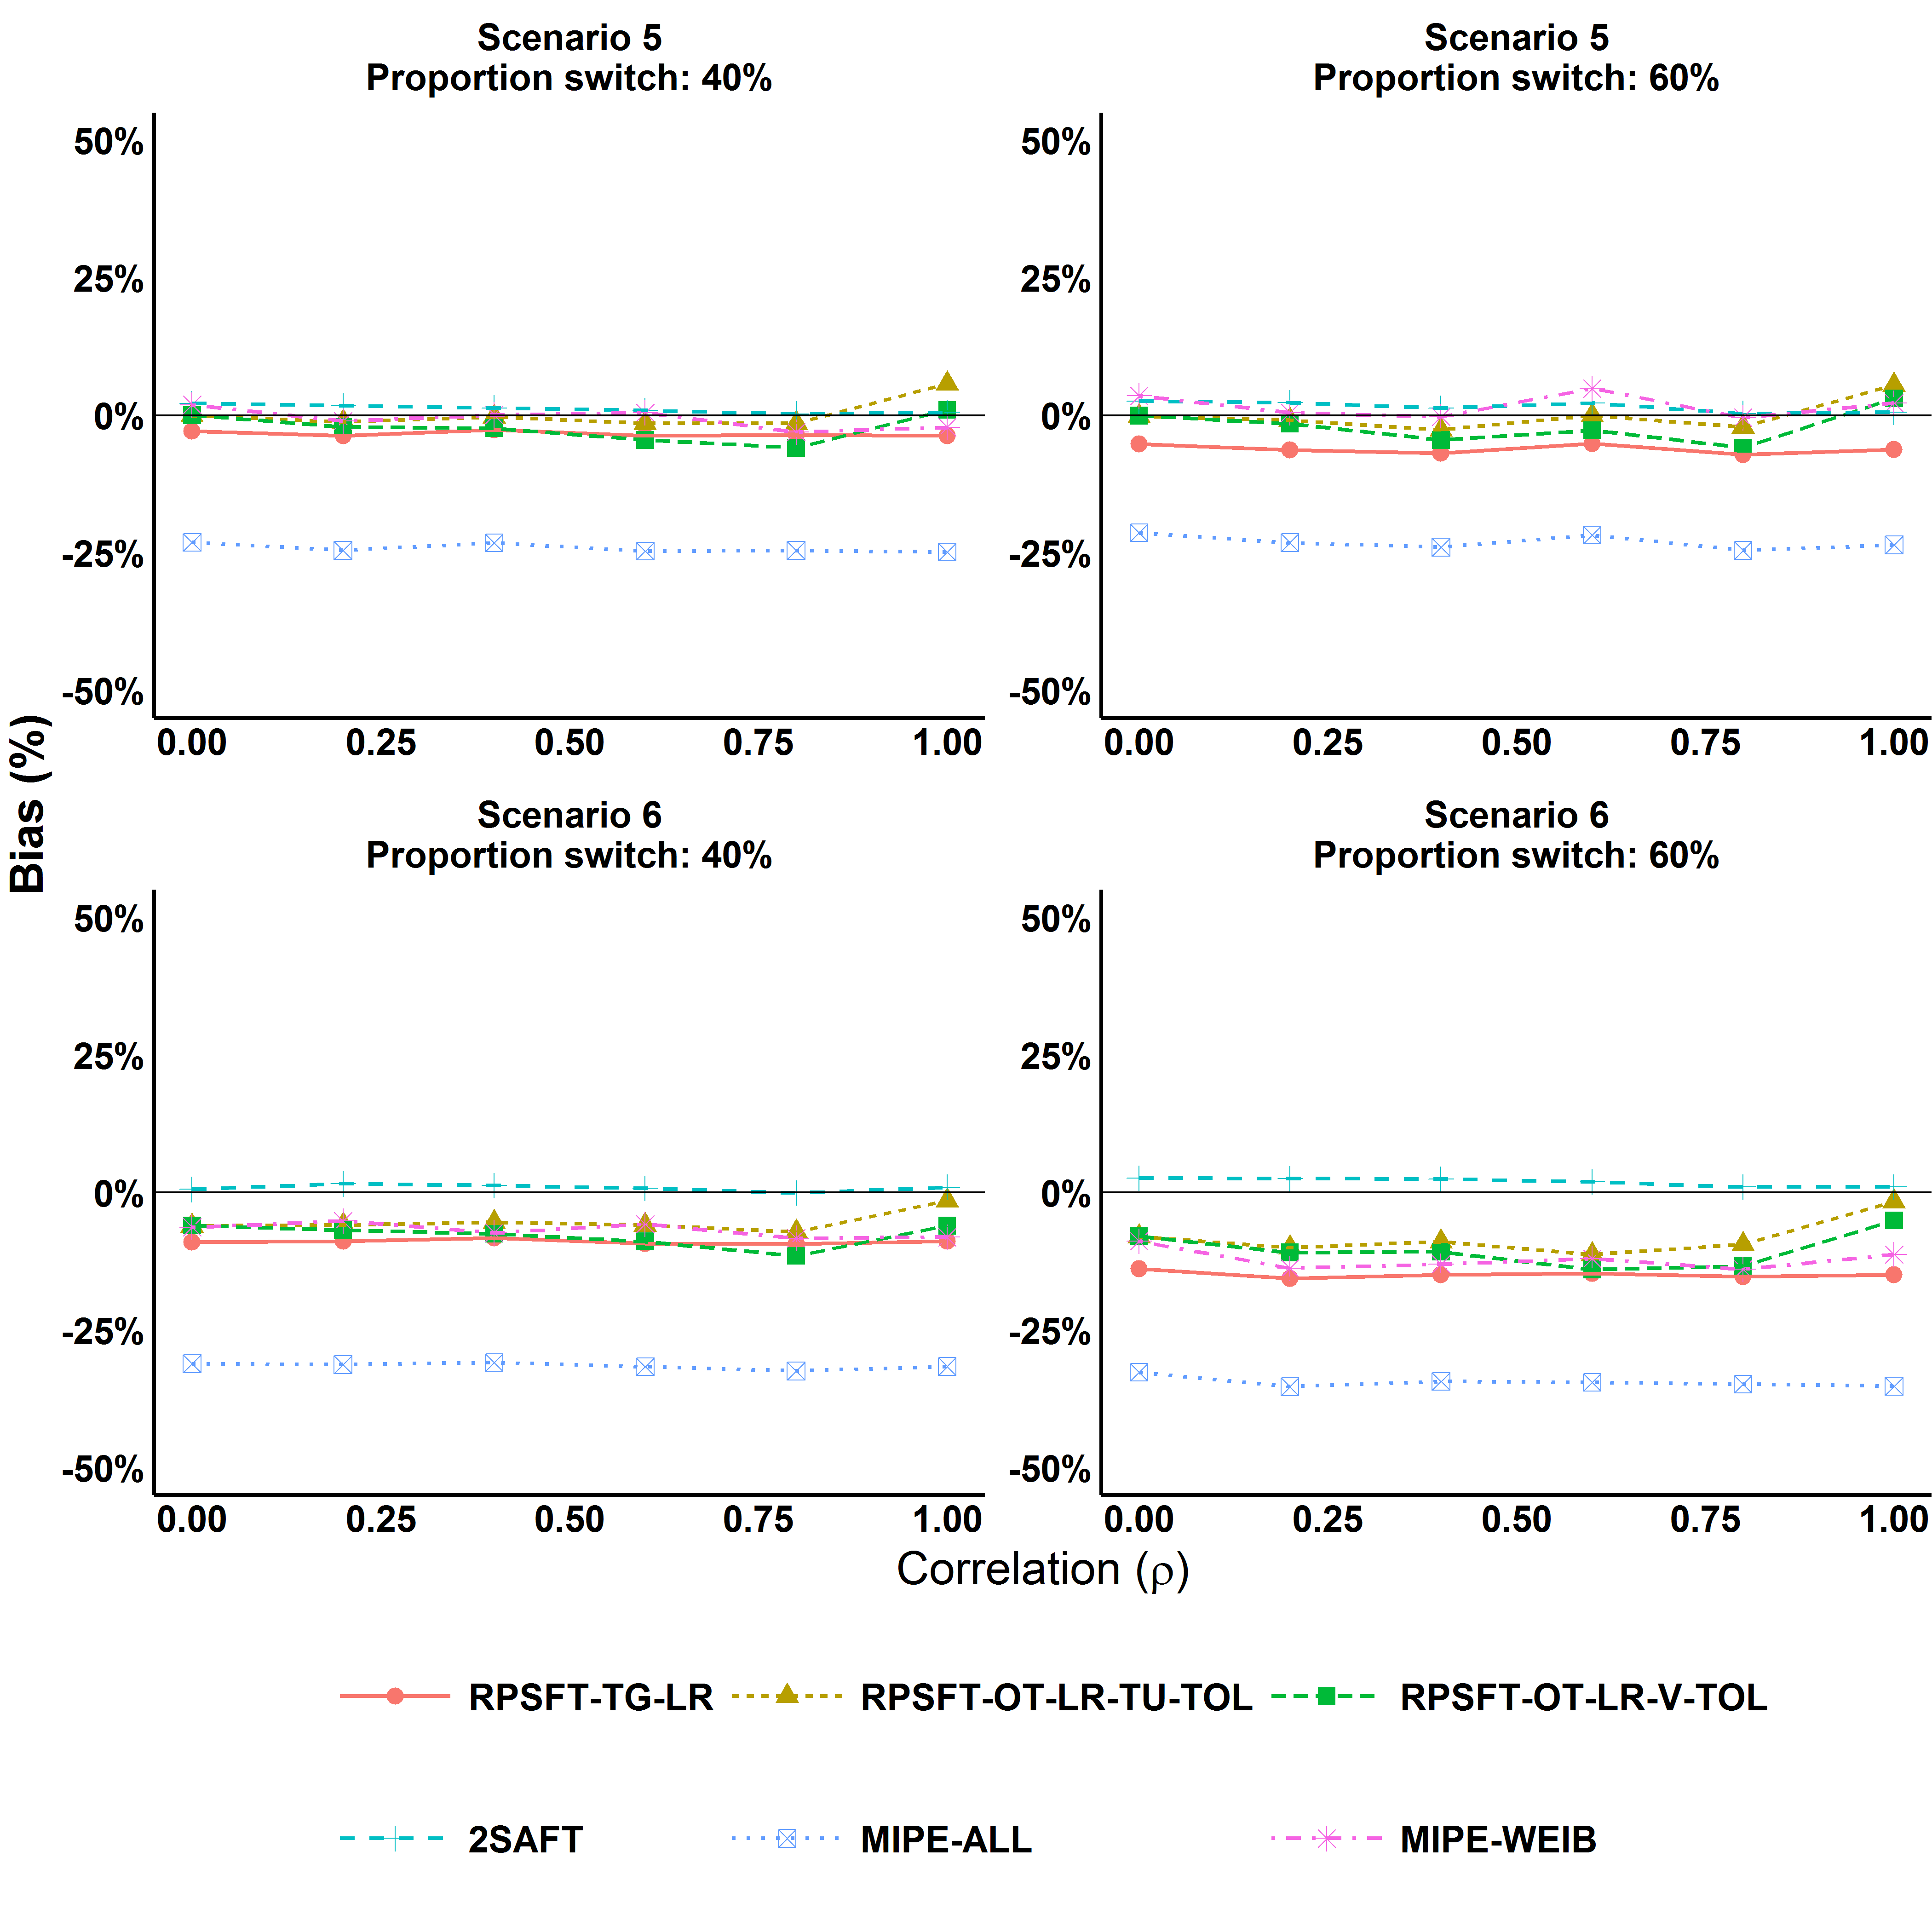
\includegraphics[width=12cm]{images/chap_sim3/comp_bias56.png}
\caption{\label{F:chap_sim3:comp_bias56} The bias for selected implementations of the complex methods for Scenario 5 and 6. In these scenarios the reduction in risk of death for switch treatment is reduced compared to the effect received as randomized treatment. As expected the rank-preserving structural failure time (RPSFT) and modified iterative parameter estimation (MIPE) methods show greater bias here than seen in the equivalent scenarios in the previous simulation study. The MIPE in general has greater bias than the RPSFT methods while the two-stage AFT (2SAFT) including recensoring and progression free survival as a covariate works well here with minimal bias.} 
\end{figure}

\clearpage

\subsection{Coverage}

Figure \ref{F:chap_sim3:simple_cov} and Figure \ref{F:chap_sim3:comp_cov} show the coverage of the confidence intervals estimated using from the simple methods and complex methods respectively. For the simple methods the coverage is very poor for the majority of the scenarios. For the RPSFT methods the correction to the confidence intervals as described in Section \ref{S:chap_methrev:RPSFTestHR} mean coverage is reasonable but not perfect. As expected the coverage for confidence intervals estimated using the MIPE method are poor and as noted by \cite{Zhang2016} there is a need for bootstrapping.

\begin{figure}[ht]
\centering
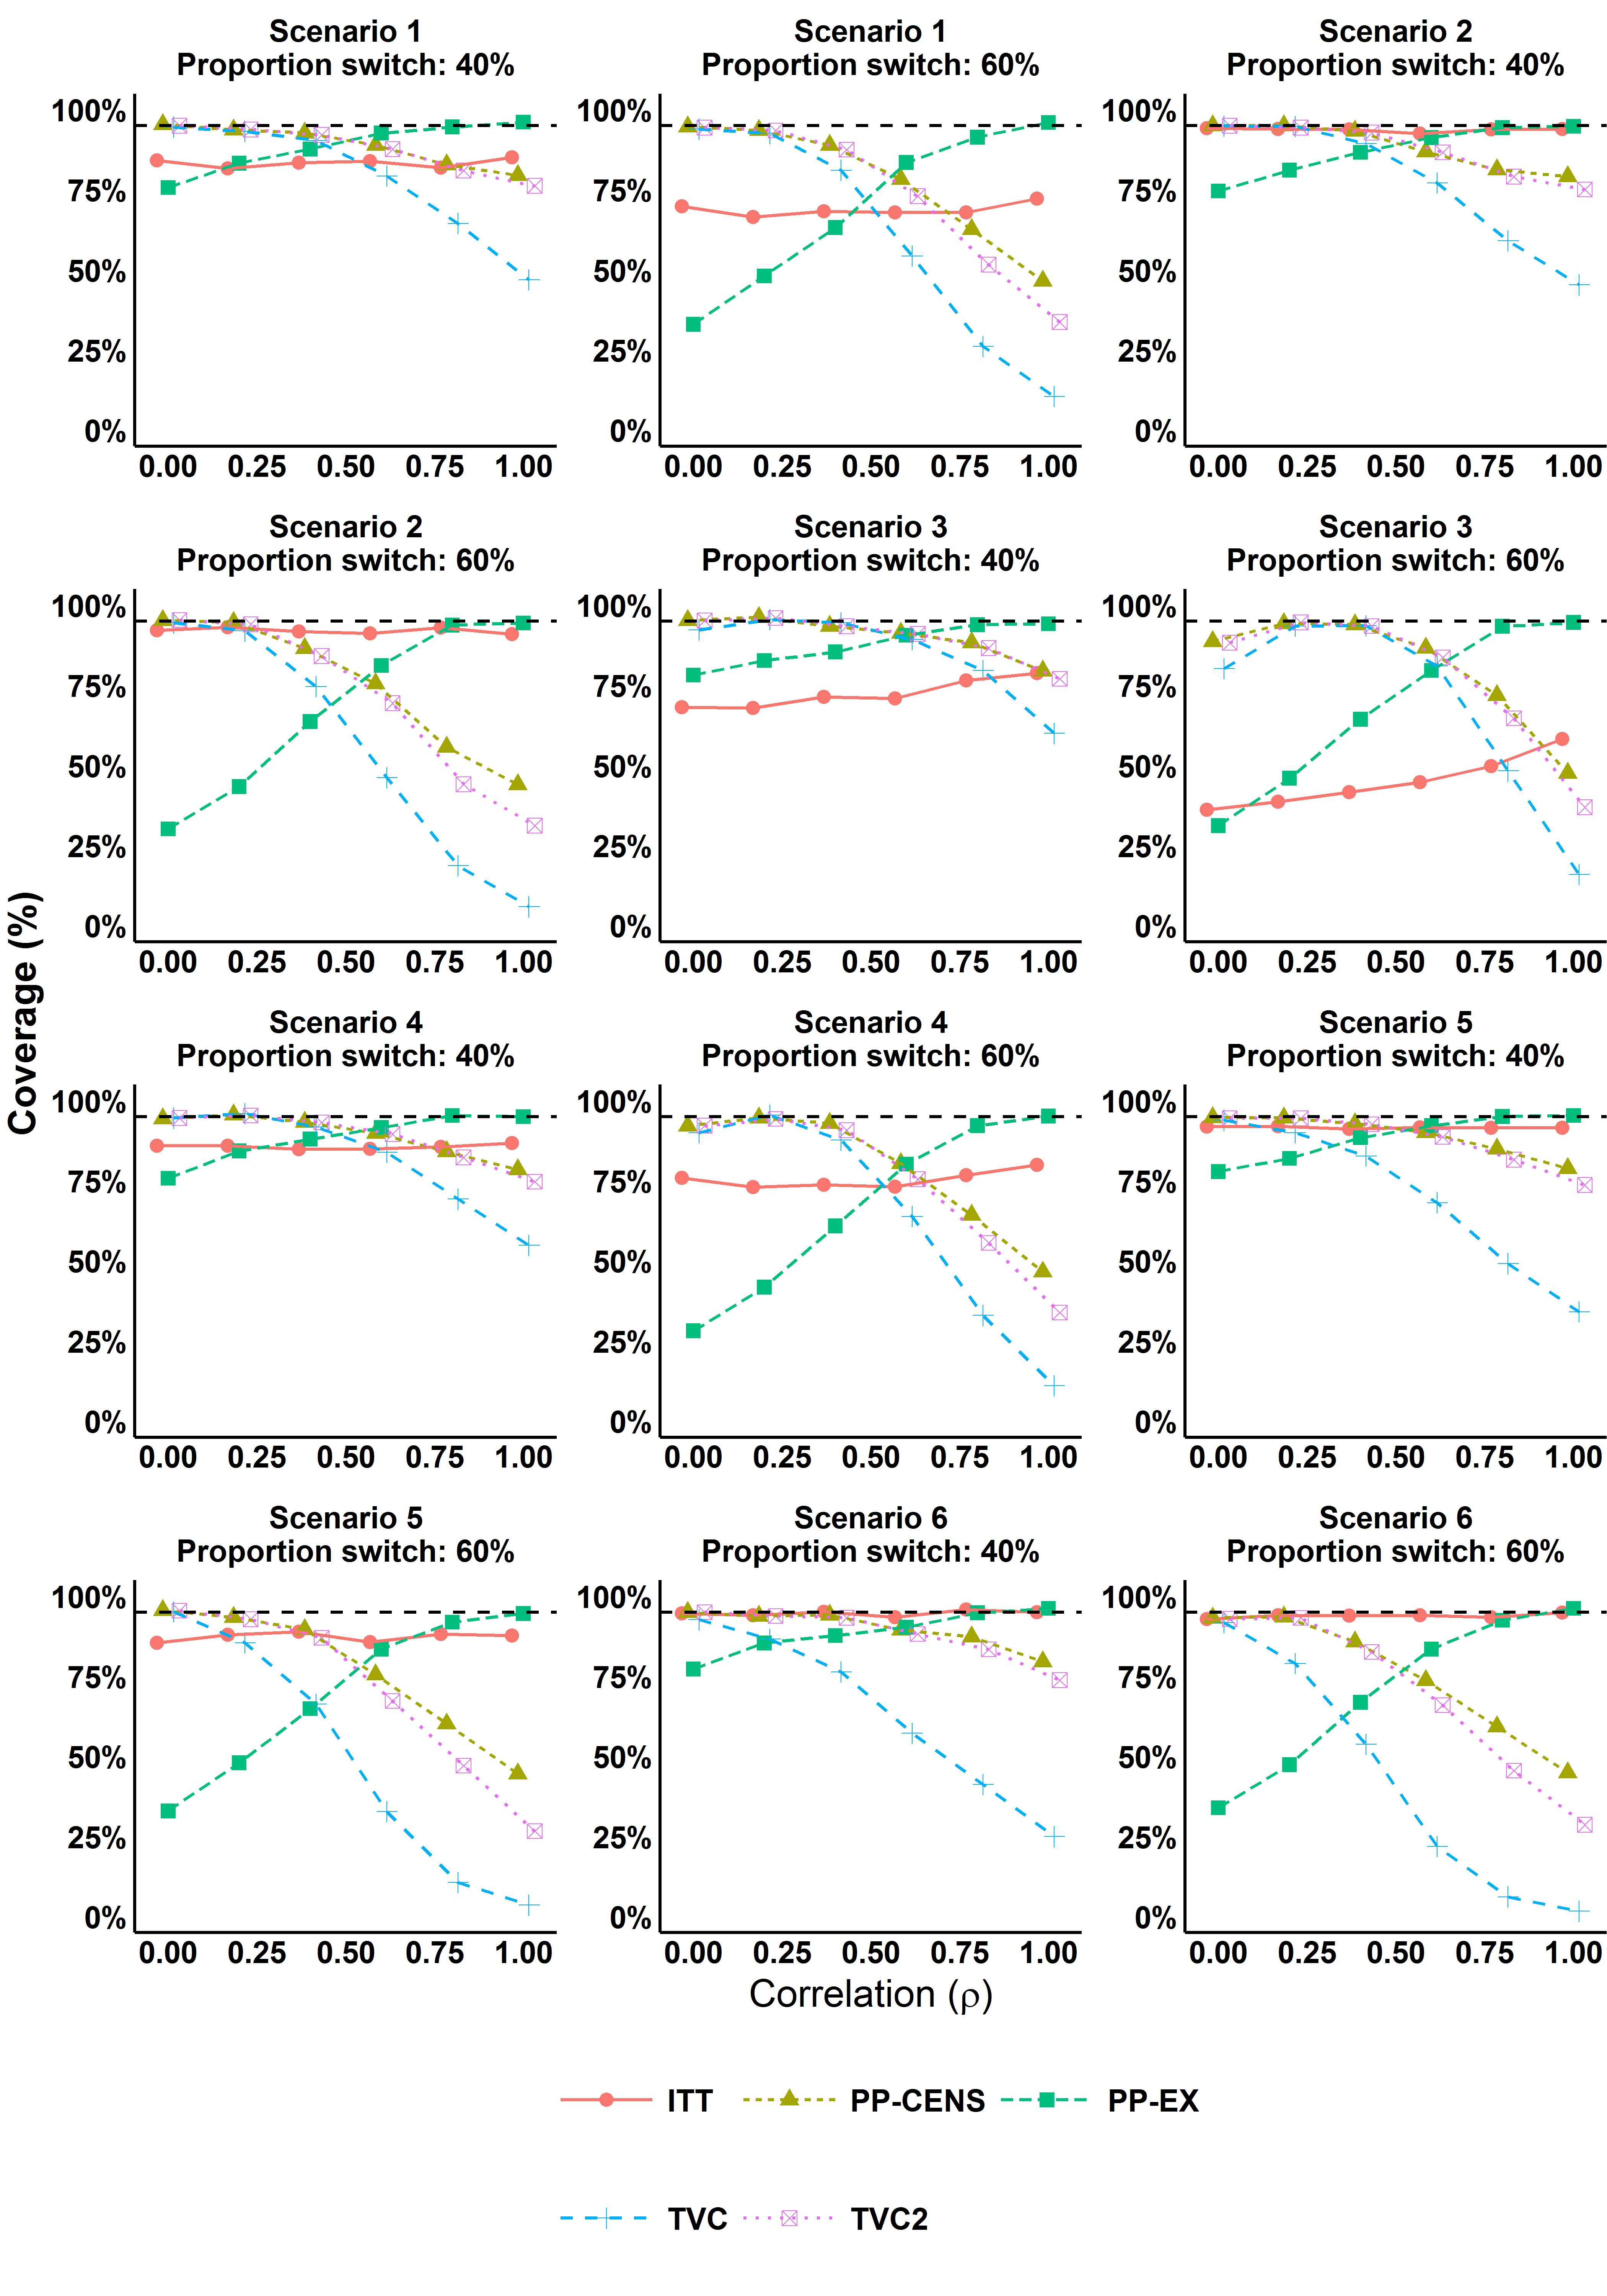
\includegraphics[width=13cm]{images/chap_sim3/simple_cov.png}
\caption{\label{F:chap_sim3:simple_cov} The coverage of the simple methods in this simulation study. The ITT performs reasonably here with a minimal coverage for the nominal 95\% confidence interval of 74.5\% that is mostly independent of correlation between time to progression and overall survival. The other methods such as treatment as a time varying covariate (TVC and TVC2) and the per-protocol analysis (PP-CENS) and (PP-EX) perform poorly. } 
\end{figure}

\begin{figure}[ht]
\centering
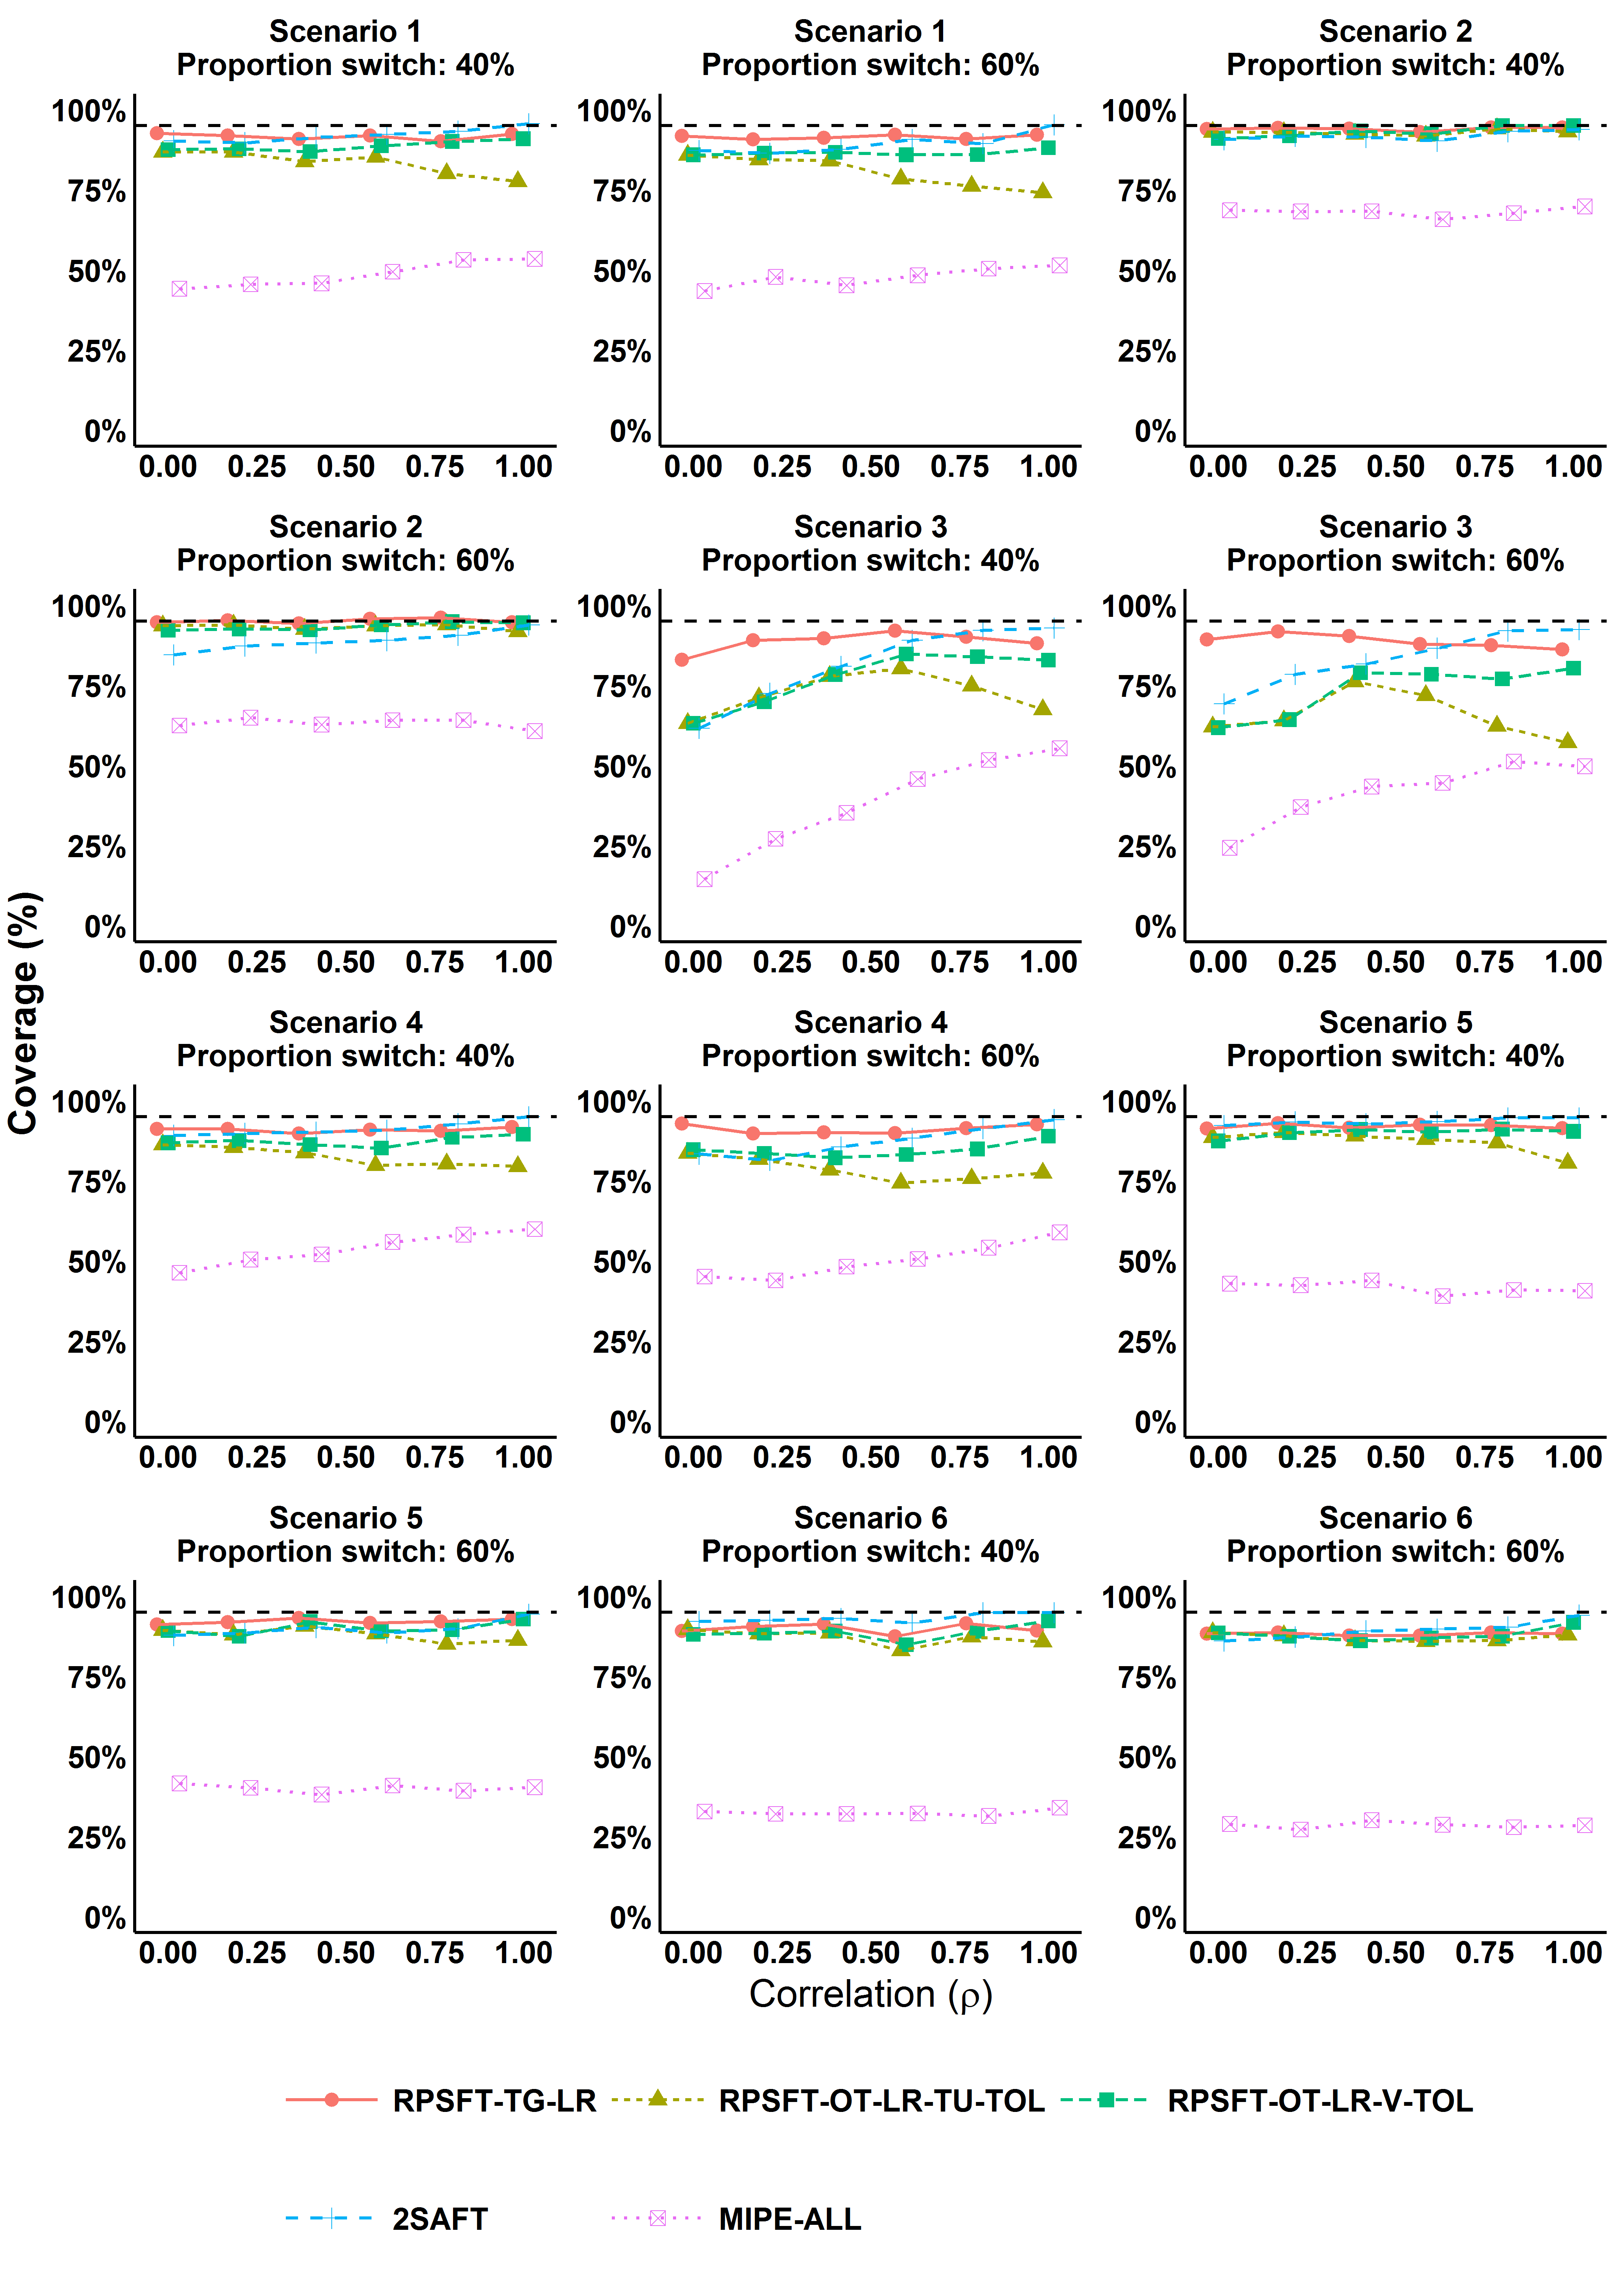
\includegraphics[width=13cm]{images/chap_sim3/comp_cov.png}
\caption{\label{F:chap_sim3:comp_cov} The coverage of the complex methods in this simulation study. For the majority of scenarios the coverage of confidence intervals for the ``treatment group'' approach to RPSFT (RPSFT-TG) using the test based correction of \cite{White1999} is acceptable. For the other RPSFT methods coverage is also reasonable but reduced relative to the ``treatment group'' approach. As expected confidence intervals for the iterative parameter estimate (MIPE) analysis have poor coverage and bootstrapping is clearly needed.} 
\end{figure}


\clearpage

\section{Conclusions of Simulation Study 2}

In this simulation study more complex patterns of treatment effect were investigated but the conclusions are very similar to those of the previous simulation study. For the per-protocol censoring at switch (PP-CENS) and both variations of treatment as a time-varying covariate (TVC and TVC2) unless there is no correlation between time to progression and overall survival the estimates of treatment effect show considerable bias. As expected the ITT analysis underestimated the treatment effect that would have been observed without switch across every scenario. The magnitude of bias depends on the magnitude of switch treatment effect with scenarios with a smaller treatment effect having smaller bias.

The two-stage AFT (2SAFT) method performs well across the majority of the 72 scenarios investigated except for a handful of the scenarios where the treatment is simulated to only have a reduction on the risk of overall survival during treatment exposure. It is unclear what causes this but it appears that it may partially be related to censoring on the counterfactual time scale.

In general the ``treatment group'' (RPSFT-TG) approach performed the best of the various flavours of RPSFT investigated with negligible differences compared to the ``on treatment'' (RPSFT-OT) approach even in scenarios that should match better to the assumptions of that model. This may be related to the convergence of the ``on treatment'' approach as the scenarios where bias was increased compared to the ``treatment group'' approach were also scenarios where the convergence was very poor for the ``on treatment'' approach. Finally even for the scenarios with a reduced effect of switch treatment violating the common treatment effect the bias was increased but not dramatically when compared to the bias observed with the simple methods. 

Once again though the value of the MIPE approach seems very limited as the bias was in some scenarios larger than observed with the RPSFT and the fact that  the convergence is worse than the ``treatment group'' approach to RPSFT and often worse than the ``on treatment'' approach suggests this method adds few benefits given the need to make additional parametric assumptions.





\chapter{Conclusion}
\label{CHAP:conclusions}

In this dissertation I have focussed on the problem of estimating a corrected\footnote{As discussed in the Section \ref{S:chap_intro:whatest} by this I mean the effect that would have been observed in the absence of treatment switching.} hazard ratio for a comparison of an experimental treatment with a control treatment in the presence of treatment switching. In Chapter \ref{CHAP:methods} I introduced the key methods that have been proposed to attempt to do this while in Chapter \ref{C:chap_sim_design} I describe a simulation study designed to test the performance of these methods when a correlation between time to progression and overall survival exists. 

\section{Results of the simulation study}

In total across the simulations in Chapter \ref{C:chap_sim2} and Chapter \ref{C:chap_sim3} 21 basis scenarios were considered as shown in Table \ref{T:chap_con:scenarios}. Of these 13 had treatment effects which, in the absence of switching, would satisfy the proportional hazards assumption underlying Cox regression. In the remaining 8 the treatment effects in the absence of switching do not meet the proportional hazards assumption but instead are potentially more realistic as they represent a treatment that either only reduces the risk of death during exposure or has a reduced residual effect after treatment stops. For these scenarios as no truth exists what is being estimated is an average hazard ratio for the duration of the trial. Finally for each of these 21 basis scenarios the correlation between time to progression and overall survival ($\rho$) was varied from 0 meaning no correlation to 1 meaning perfect correlation across 6 levels leading to 126 scenarios. It should be noted that while I simulate scenarios with no correlation and perfect correlation these are extreme scenarios and based on the review of \cite{Ciani2014} discussed in Section \ref{S:chap_intro:correlation} only results for scenarios with correlation between 0.4 and 0.8 can be considered realistic and are presented in Appendix \ref{A:allres} and will be discussed here.

\begin{table}
\caption{Basis scenario descriptions\label{T:chap_con:scenarios}}
\begin{tabular}{lll}
\hline
\hline
Basis    & Simulation  & Description  \\ 
Scenario & Study       &        \\
  \hline
 1 & Study 1 & True Hazard Ratio: 0.7, Proportion switch: 20\% \\ 
 2 & Study 1 & True Hazard Ratio: 0.7, Proportion switch: 40\% \\ 
 3 & Study 1 &  True Hazard Ratio: 0.7, Proportion switch: 60\% \\ 
 4 & Study 1 & True Hazard Ratio: 0.9, Proportion switch: 20\% \\ 
 5 & Study 1 & True Hazard Ratio: 0.9, Proportion switch: 40\% \\
 6 & Study 1 & True Hazard Ratio: 0.9, Proportion switch: 60\% \\ 
 7 & Study 1 & True Hazard Ratio: 1, Proportion switch: 20\% \\ 
 8 & Study 1 & True Hazard Ratio: 1, Proportion switch: 40\% \\ 
 9 & Study 1 &  True Hazard Ratio: 1, Proportion switch: 60\% \\ 
 \hline
 10  & Study 2 & Scenario 1, Proportion switch: 40\% \\ 
 11  & Study 2 & Scenario 1, Proportion switch: 60\% \\ 
 12  & Study 2 & Scenario 2, Proportion switch: 40\% \\ 
 13  & Study 2 & Scenario 2, Proportion switch: 60\% \\ 
 14 & Study 2 & Scenario 3, Proportion switch: 40\% \\ 
 15 & Study 2 & Scenario 3, Proportion switch: 60\% \\ 
 16 & Study 2 & Scenario 4, Proportion switch: 40\% \\ 
 17  & Study 2 & Scenario 4, Proportion switch: 60\% \\ 
 18  & Study 2 & Scenario 5, Proportion switch: 40\% \\ 
 19  & Study 2 & Scenario 5, Proportion switch: 60\% \\ 
 20  & Study 2 & Scenario 6, Proportion switch: 40\% \\ 
 21  & Study 2 & Scenario 6, Proportion switch: 60\% \\ 
\hline
\end{tabular}
\end{table}


\subsection{Bias of the simple methods}

With regards to the bias of the simple methods my findings align closely with \cite{Morden2011}, \cite{Latimer2013} and \cite{Latimer2016}. Similar to these published studies, though assessing different outcomes, I found that all of the simple methods perform badly when the correlation between time to progression and overall survival is at a realistic level. This can be seen in Figure \ref{F:allp:simple}. The main difference between my findings and the prior simulations is that in this study this bias was observed without making any assumptions on the prognosis of switchers vs non-switchers. This is important as it avoids what \cite{Slaets2013} describe as the ``Can of worms'' of making judgements on how selective switching is.

\subsection{Performance of the RPSFT}

In Chapter \ref{CHAP:methods} I discussed that there were a selection of choices to be made when using the RPSFT method including choice of test for g-estimation, the choice of ``treatment group'' or ``on treatment'' model and whether hazard ratios are estimated from a comparison of observed and latent survival times or from a comparison of counterfactual and latent survival times. 

With reference to Figure \ref{F:allp:rpsft} it is clear that the the choice of test has minimal effect in these simulations as does the choice on how to estimate a corrected hazard ratio. With regards to the choice of ``treatment group'' vs ``on treatment'' across many of the simulations the choice also has negligible impact. In basis scenarios 1-9 the ``treatment group'' approach has lower bias where the data is generated consistently with this assumption. Surprisingly this is also the case with basis scenarios 10-17 where the true treatment effect was simulated to apply either only or with greater effect during treatment. In fact the only scenarios where the ``on treatment'' approach has lower bias is in basis scenarios 18-21 where the switch treatment had lower effect violating the common treatment effect assumption. Given this and the issues with convergence of the ``on treatment'' approach as discussed in Section \ref{S:chap_sim3:gest} it seems reasonable to in general use the ``treatment group'' approach as a main analysis with the ``on treatment'' considered a sensitivity if it converges. 


While the bias is acceptable across the majority of scenarios it can be seen that scenarios 15, 17 and 21 all show high levels of bias. Though for 15 and 17 still much lower than observed with the ITT analysis. These are all scenarios with a high degree of switching (60\% of control patients switch) and with switch effect that is potentially different between randomized patients and switch patients. This result is consistent with \cite{Latimer2013} and \cite{Latimer2016} where violations of the common treatment effect were found to increase the bias of the RPSFT approach. 

\subsection{Performance of the MIPE}

The biggest surprise with this simulation study has been the poor performance of the modified IPE method described in Section \ref{S:chap_methrev:MIPE}. As can be seen in Figure \ref{F:allp:mipe} across a large number of scenarios investigated the bias is considerably larger than that from the RPSFT methods with no predictable pattern. In addition the convergence of this method was generally much lower than the RPSFT. This is quite different to the findings of \cite{Morden2011}, \cite{Latimer2013} and \cite{Latimer2016} who generally found it to have comparable or better performance than the RPSFT. It is unclear what the cause of these differences are though a few differences between the simulations exist:
\begin{enumerate}
\item The datasets simulated have far greater censoring of overall survival. As can be seen in the sample curves presented in Figure \ref{F:chap_sim_design:exampleKM} compared to the 21\% administrative censoring reported by e.g. \cite{Latimer2013}. 
\item The application of treatment effects is different with \cite{Morden2011} applying treatment as a causal acceleration factor, while I apply a reduction in hazard.
\end{enumerate}
Finally despite the change in name it seems unlikely there are differences in methodology as the modification to the censoring algorithm described by \cite{Zhang2016} for the modified IPE matches to the censoring approach described by \cite{Latimer2016}. 
Further investigation of this method is needed to understand under which scenarios the IPE does perform well though given the additional parametric assumptions it is hard to see the benefits of this method compared to the RPSFT approach. 

\subsection{Performance of the Two-stage AFT}

Figure \ref{F:allp:saft} shows that similarly to the findings of \cite{Latimer2013} and \cite{Latimer2016} the simple two stage approach has very low bias across the majority of scenarios. However, even this method exhibited important bias of greater than 10\% in Scenario 14 and 15. These are scenarios where the treatment effect only yielded a reduction in the hazard of death during treatment with a reversion to baseline hazard after treatment stopped. Combined with the larger amounts of censoring in this simulation study compared to the 21\% censoring of \cite{Latimer2013} seems to lead to a situation where the two-stage AFT method is less robust than previously seen. Given the low bias across the remainder of the scenarios further investigation of this method seems warranted. As seen in Section \ref{S:chap_intro:pattern} the required pattern of switching only at progression is not uncommon within oncology trials.

\section{Limitations of this study}

As with all simulation studies only a finite number of scenarios can be investigated and by focusing on the impact of correlation between time to progression and overall survival the impact of prognostic covariates was ignored. While this is helpful in order to show that the simple methods are very biased without having to make any further assumptions on prognosis it is clearly unrealistic. The most important aspect that is missing from the simulation framework used here are time dependent prognostic covariates that jointly affect progression and survival. Given the complexity of deriving appropriate inverse hazard functions even for the simple scenarios here with only time dependent treatment covariates it is likely that numerical methods would have to employed to simulate such survival times. 

The second major limitation which in many ways is a consequence of the first is that the IPCW method was not assessed in any of the scenarios. As this method requires the presence of time varying covariates to be applied it was not possible to be considered here. 

The final major limitation is the choice of hazard ratio as the outcome of interest. While by far the most commonly reported measure of treatment effect in the survival analysis of clinical trials the use of Cox regression to estimate effects when the proportional hazards assumption is violated is also subject to bias.

\section{Conclusion}

This dissertation has investigated the impact on trial results assuming that treatment switching is an unavoidable aspect of oncology clinical trials when in reality it is a design choice. The simulations performed here suggest that when this design choice is made statistical modelling can attempt to provide a reasonable estimate of the treatment effect in the absence of switch. However, even the best performing methods (the two-stage AFT and the ``treatment group'' RPSFT) in at least one realistic scenario over estimated the treatment effect by greater than 10\% and the only design choice that will guarantee an unbiased estimate of overall survival treatment effect would be to forbid switching. However, as noted by \cite{Prasad2014} this is an ethical as well as technical decision. 
\begin{quote}
Ethically, benefits to participants should be maximized but should not compromise the scientific validity of a study. In an effort to offer the hope of benefit to ill participants in the control arm, oncology investigators often build in an option for participants who progress to cross over to the experimental arm. This carries the implicit assumption that the investigational agent is beneficial, subverting the concept of true clinical equipoise.
\end{quote}
Whether a moderate increase in uncertainty in the estimate of what may be a secondary endpoint of a clinical trial justifies preventing access to a potentially beneficial experimental therapy when no alternatives exist is a challenging ethical question. It should also be noted that even if the decision is made to forbid treatment switching until equipoise is disturbed at an interim analysis then these adjustment methods will still be required for later analyses as discussed in Section \ref{S:chap_intro:pattern}. 

Regardless of the design decision made this study combined with evidence from prior simulations makes it clear that simple methods should be avoided and that two-stage AFT or RPSFT method should be considered alongside the ITT analysis when analysing trials where treatment switching has occurred if the aim is to estimate what the treatment effect would have been in the absence of switching. 


%%%%%%%%%%%%%%%%%%%%%%%%%%%%%%%%%%%%%%%%%%%%%%%%%%%%
%%%%%%%%%%%%%%%%%%%%%%%%%%%%%%%%%%%%%%%%%%%%%%%%%%%%
\clearpage

\bibliography{References}
\addcontentsline{toc}{chapter}{References}
\bibliographystyle{somas}

%%%%%%%%%%%%%%%%%%%%%%%%%%%%%%%%%%%%%%%%%%%%%%%%%%%%
\clearpage
\appendix

\chapter{Additional plots for all simulations}

\label{A:allres}
This Appendix contains additional plots showing combined results of Simulation Study 1 described in Chapter \ref{C:chap_sim2} and Simulation Study 2 described in Chapter \ref{C:chap_sim3}. Based on Section \ref{S:chap_intro:correlation} and \cite{Ciani2014} only results for a realistic range for the correlation between time to progression and overall survival are presented in this Appendix. That is only the correlations of 0.4, 0.6 and 0.8 are presented here. Care should be taken when examining these plots as the y axis are not constant. Table \ref{T:chap_con:scenarios} shows the description for each of the 21 basis scenarios.

\clearpage

\begin{sidewaysfigure}
    \centering
    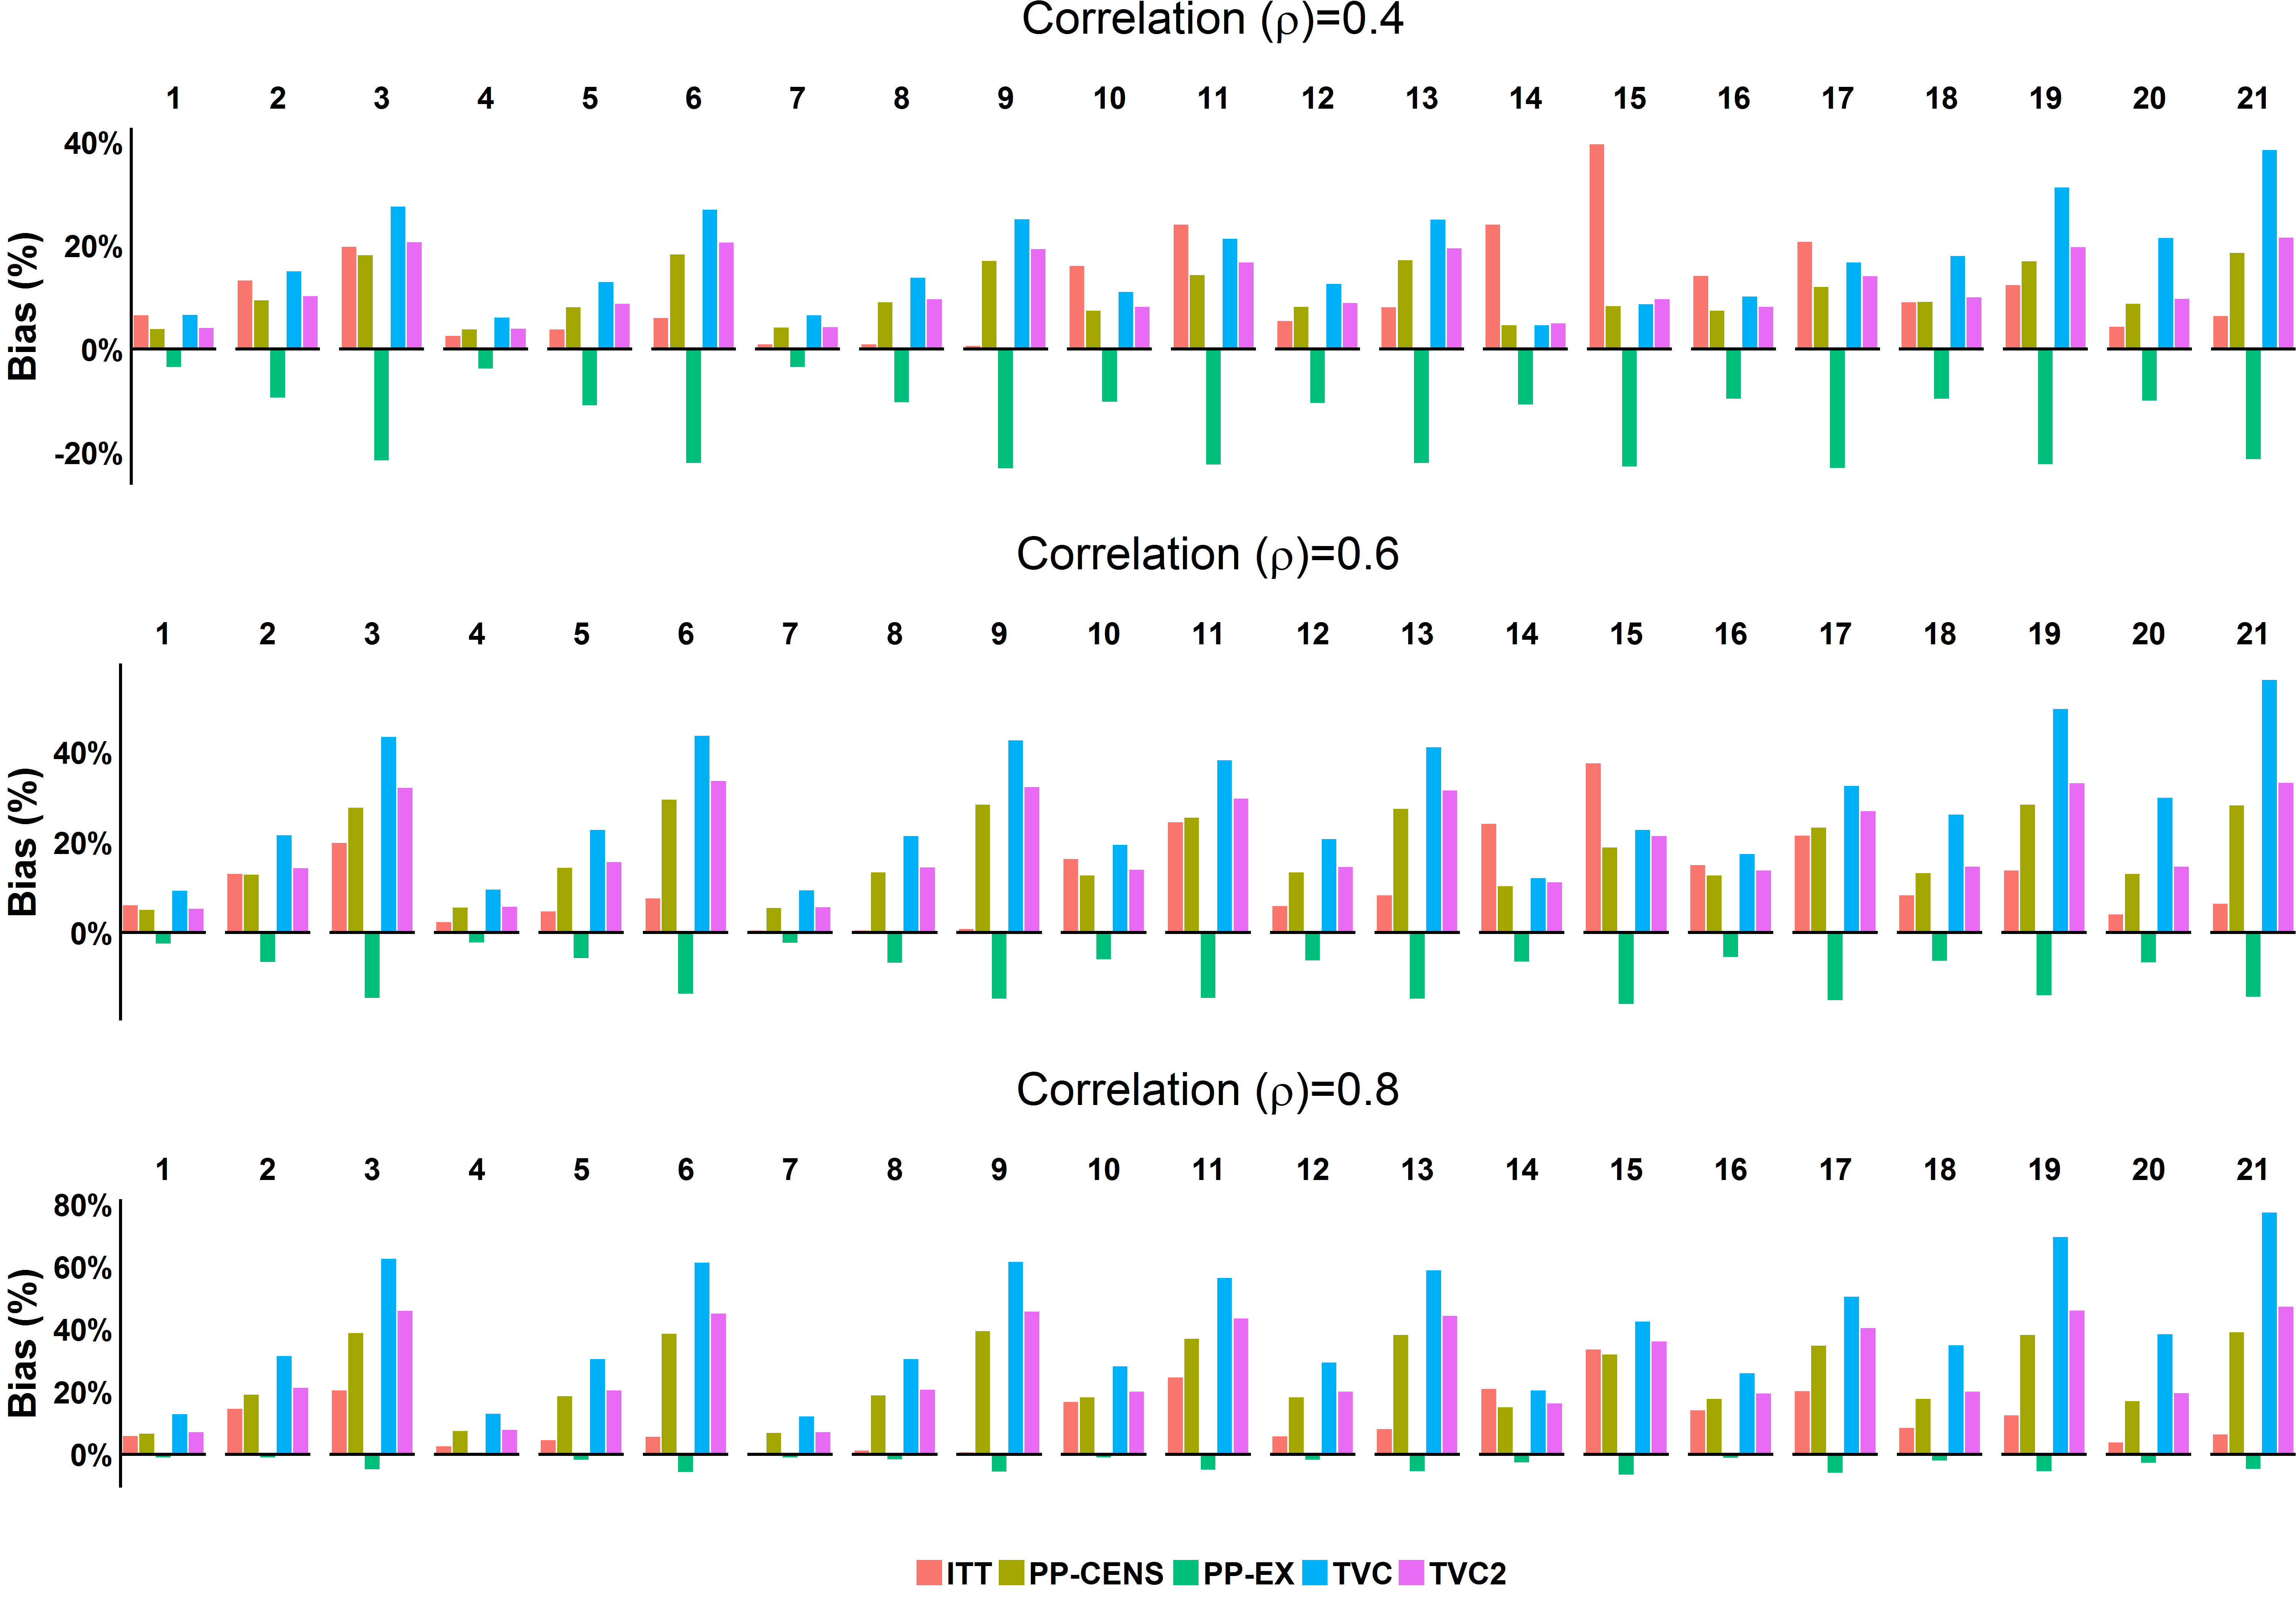
\includegraphics[width=20cm]{images/app_allres/simp_bias4.png}
    \caption{The percentage bias across all simulations for the simple methods. \\ ITT = Intent to treat analysis; PP-CENS = Per-protocol censoring at switch; PP-EX = Per-protocol excluding switchers; TVC = Treatment as a time-varying covariate; TVC2 = Switch treatment as a time-varying covariate}
    \label{F:allp:simple}
\end{sidewaysfigure}

\begin{sidewaysfigure}
    \centering
    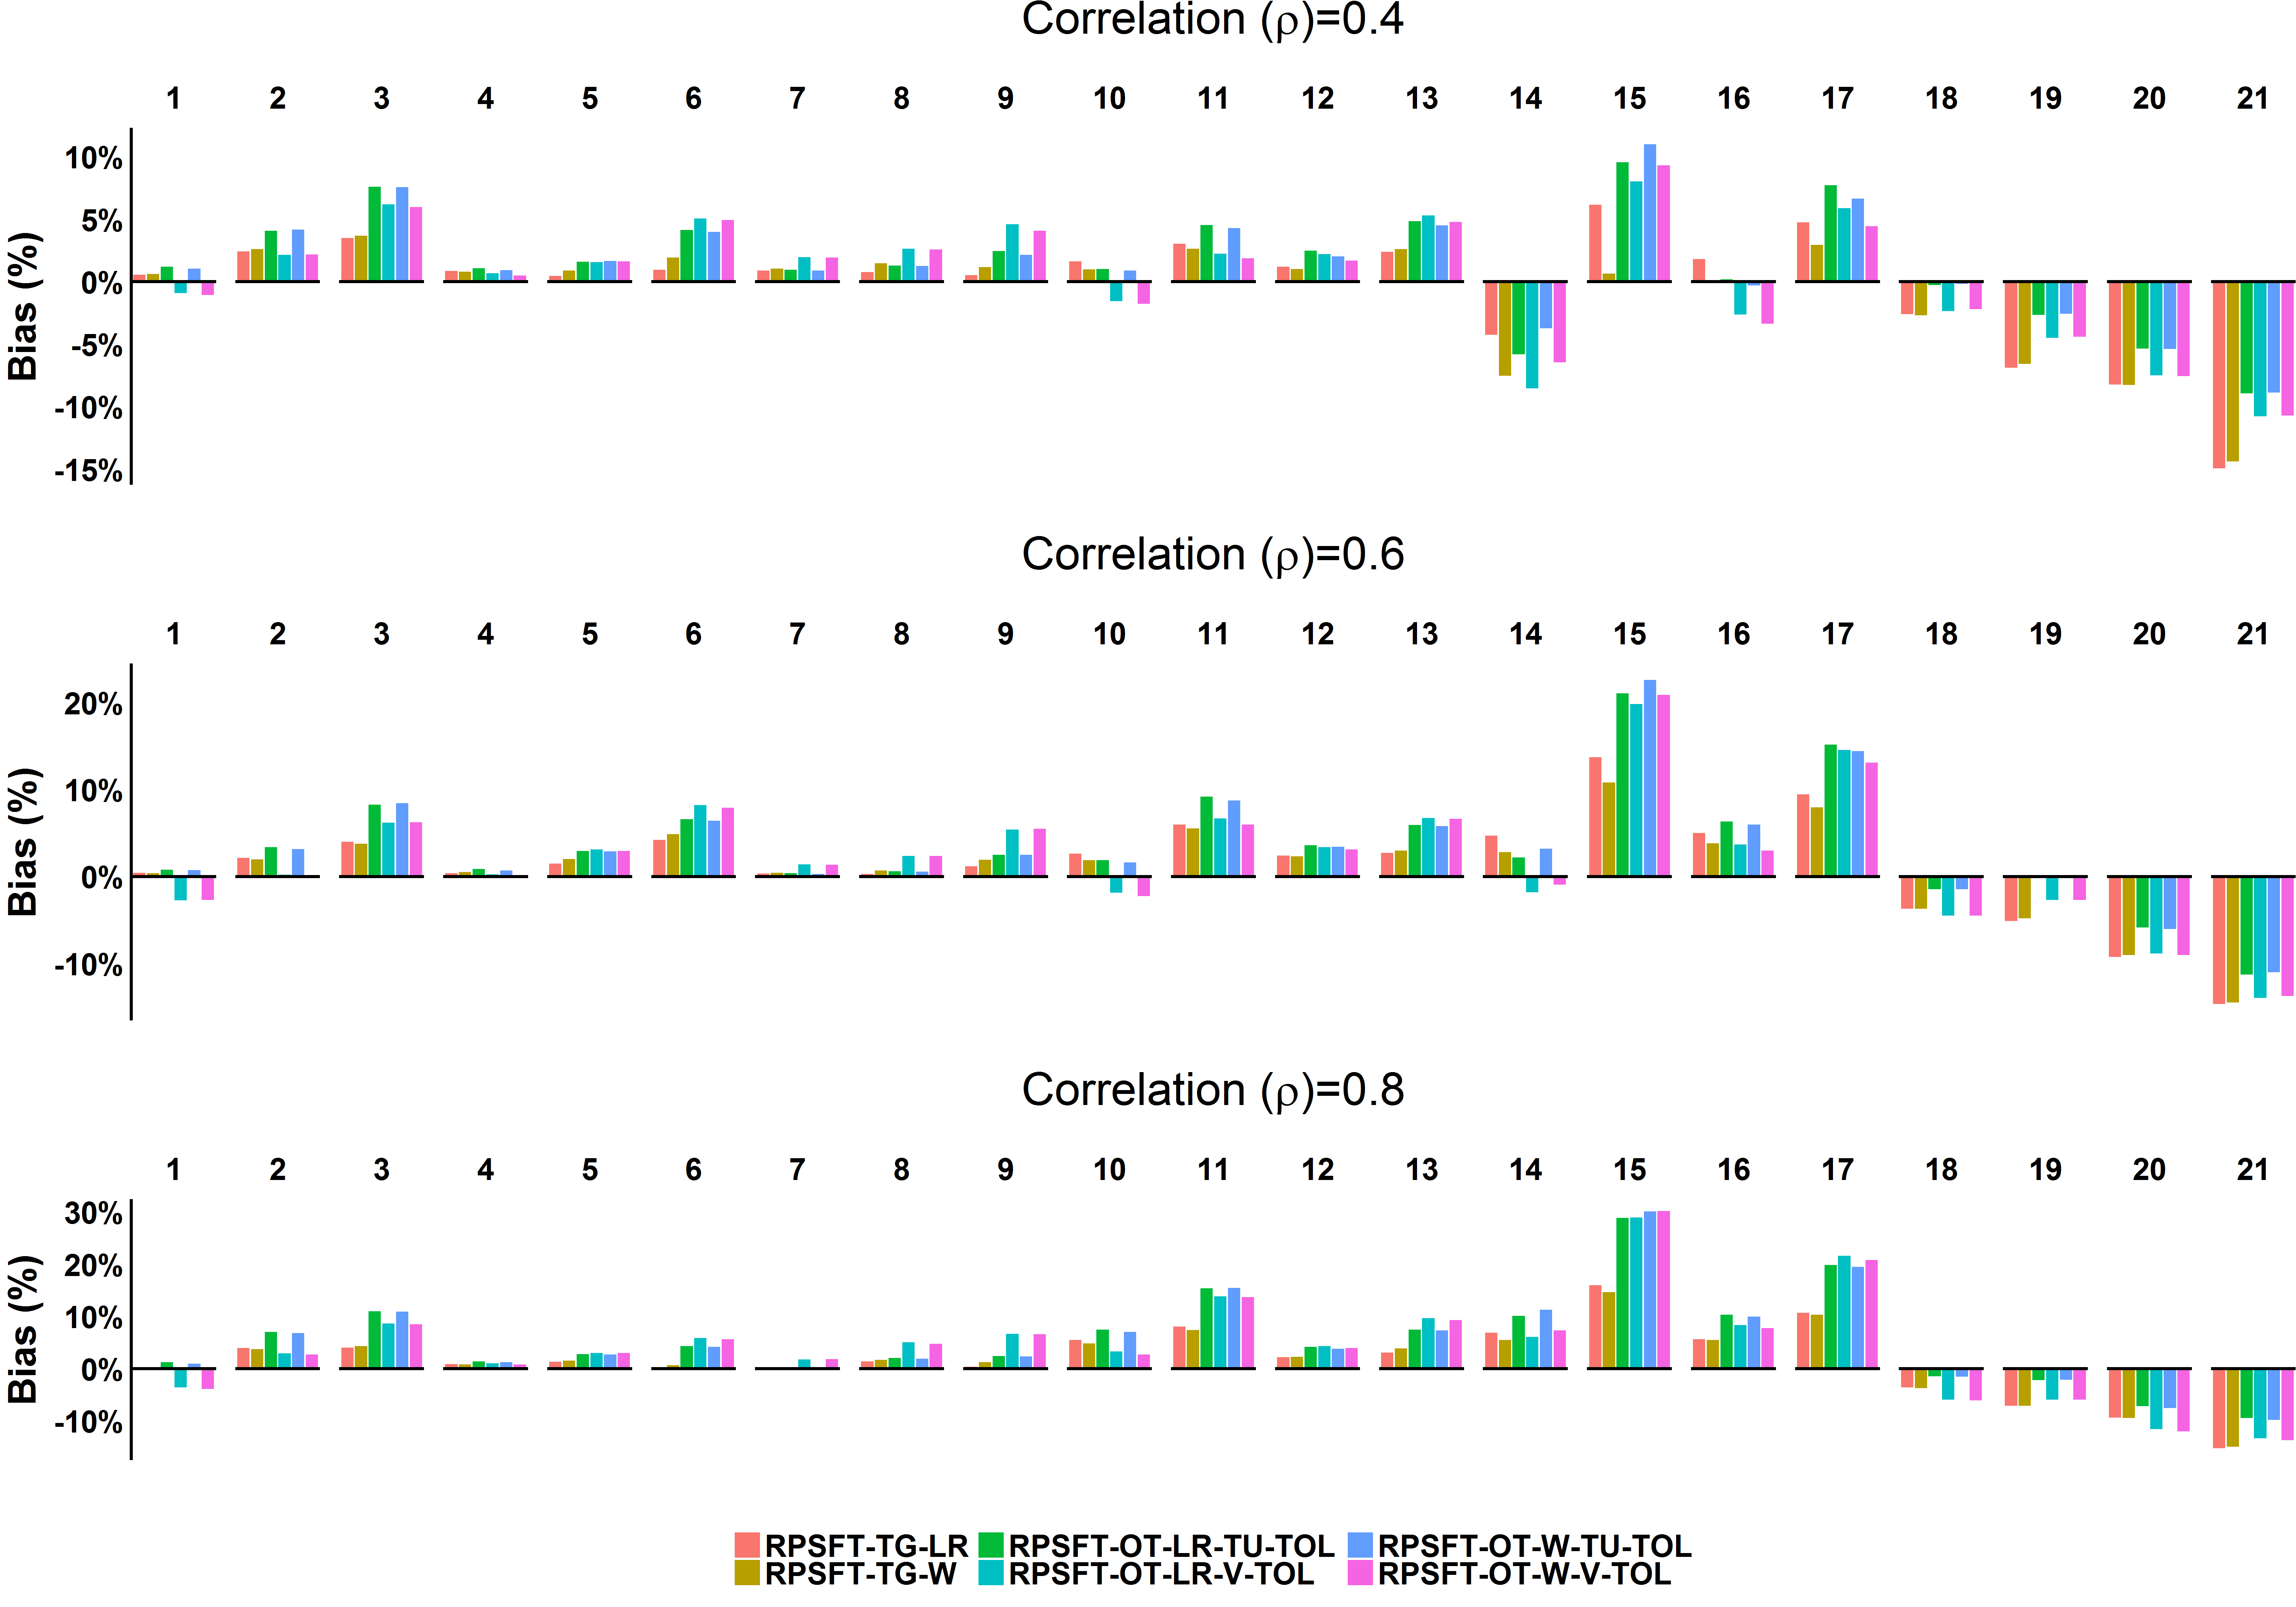
\includegraphics[width=20cm]{images/app_allres/rpsft_bias4.png}
    \caption{The percentage bias across all simulations for variations on the RPSFT method. \\ TG = ``treatment group''; OT = ``on treatment''; LR = log-rank test; W = wilcoxon test; TU = hazard ratio estimated as observed vs latent; V = hazard ratio estimated as counterfactual vs latent}
    \label{F:allp:rpsft}
\end{sidewaysfigure}

\begin{sidewaysfigure}
    \centering
    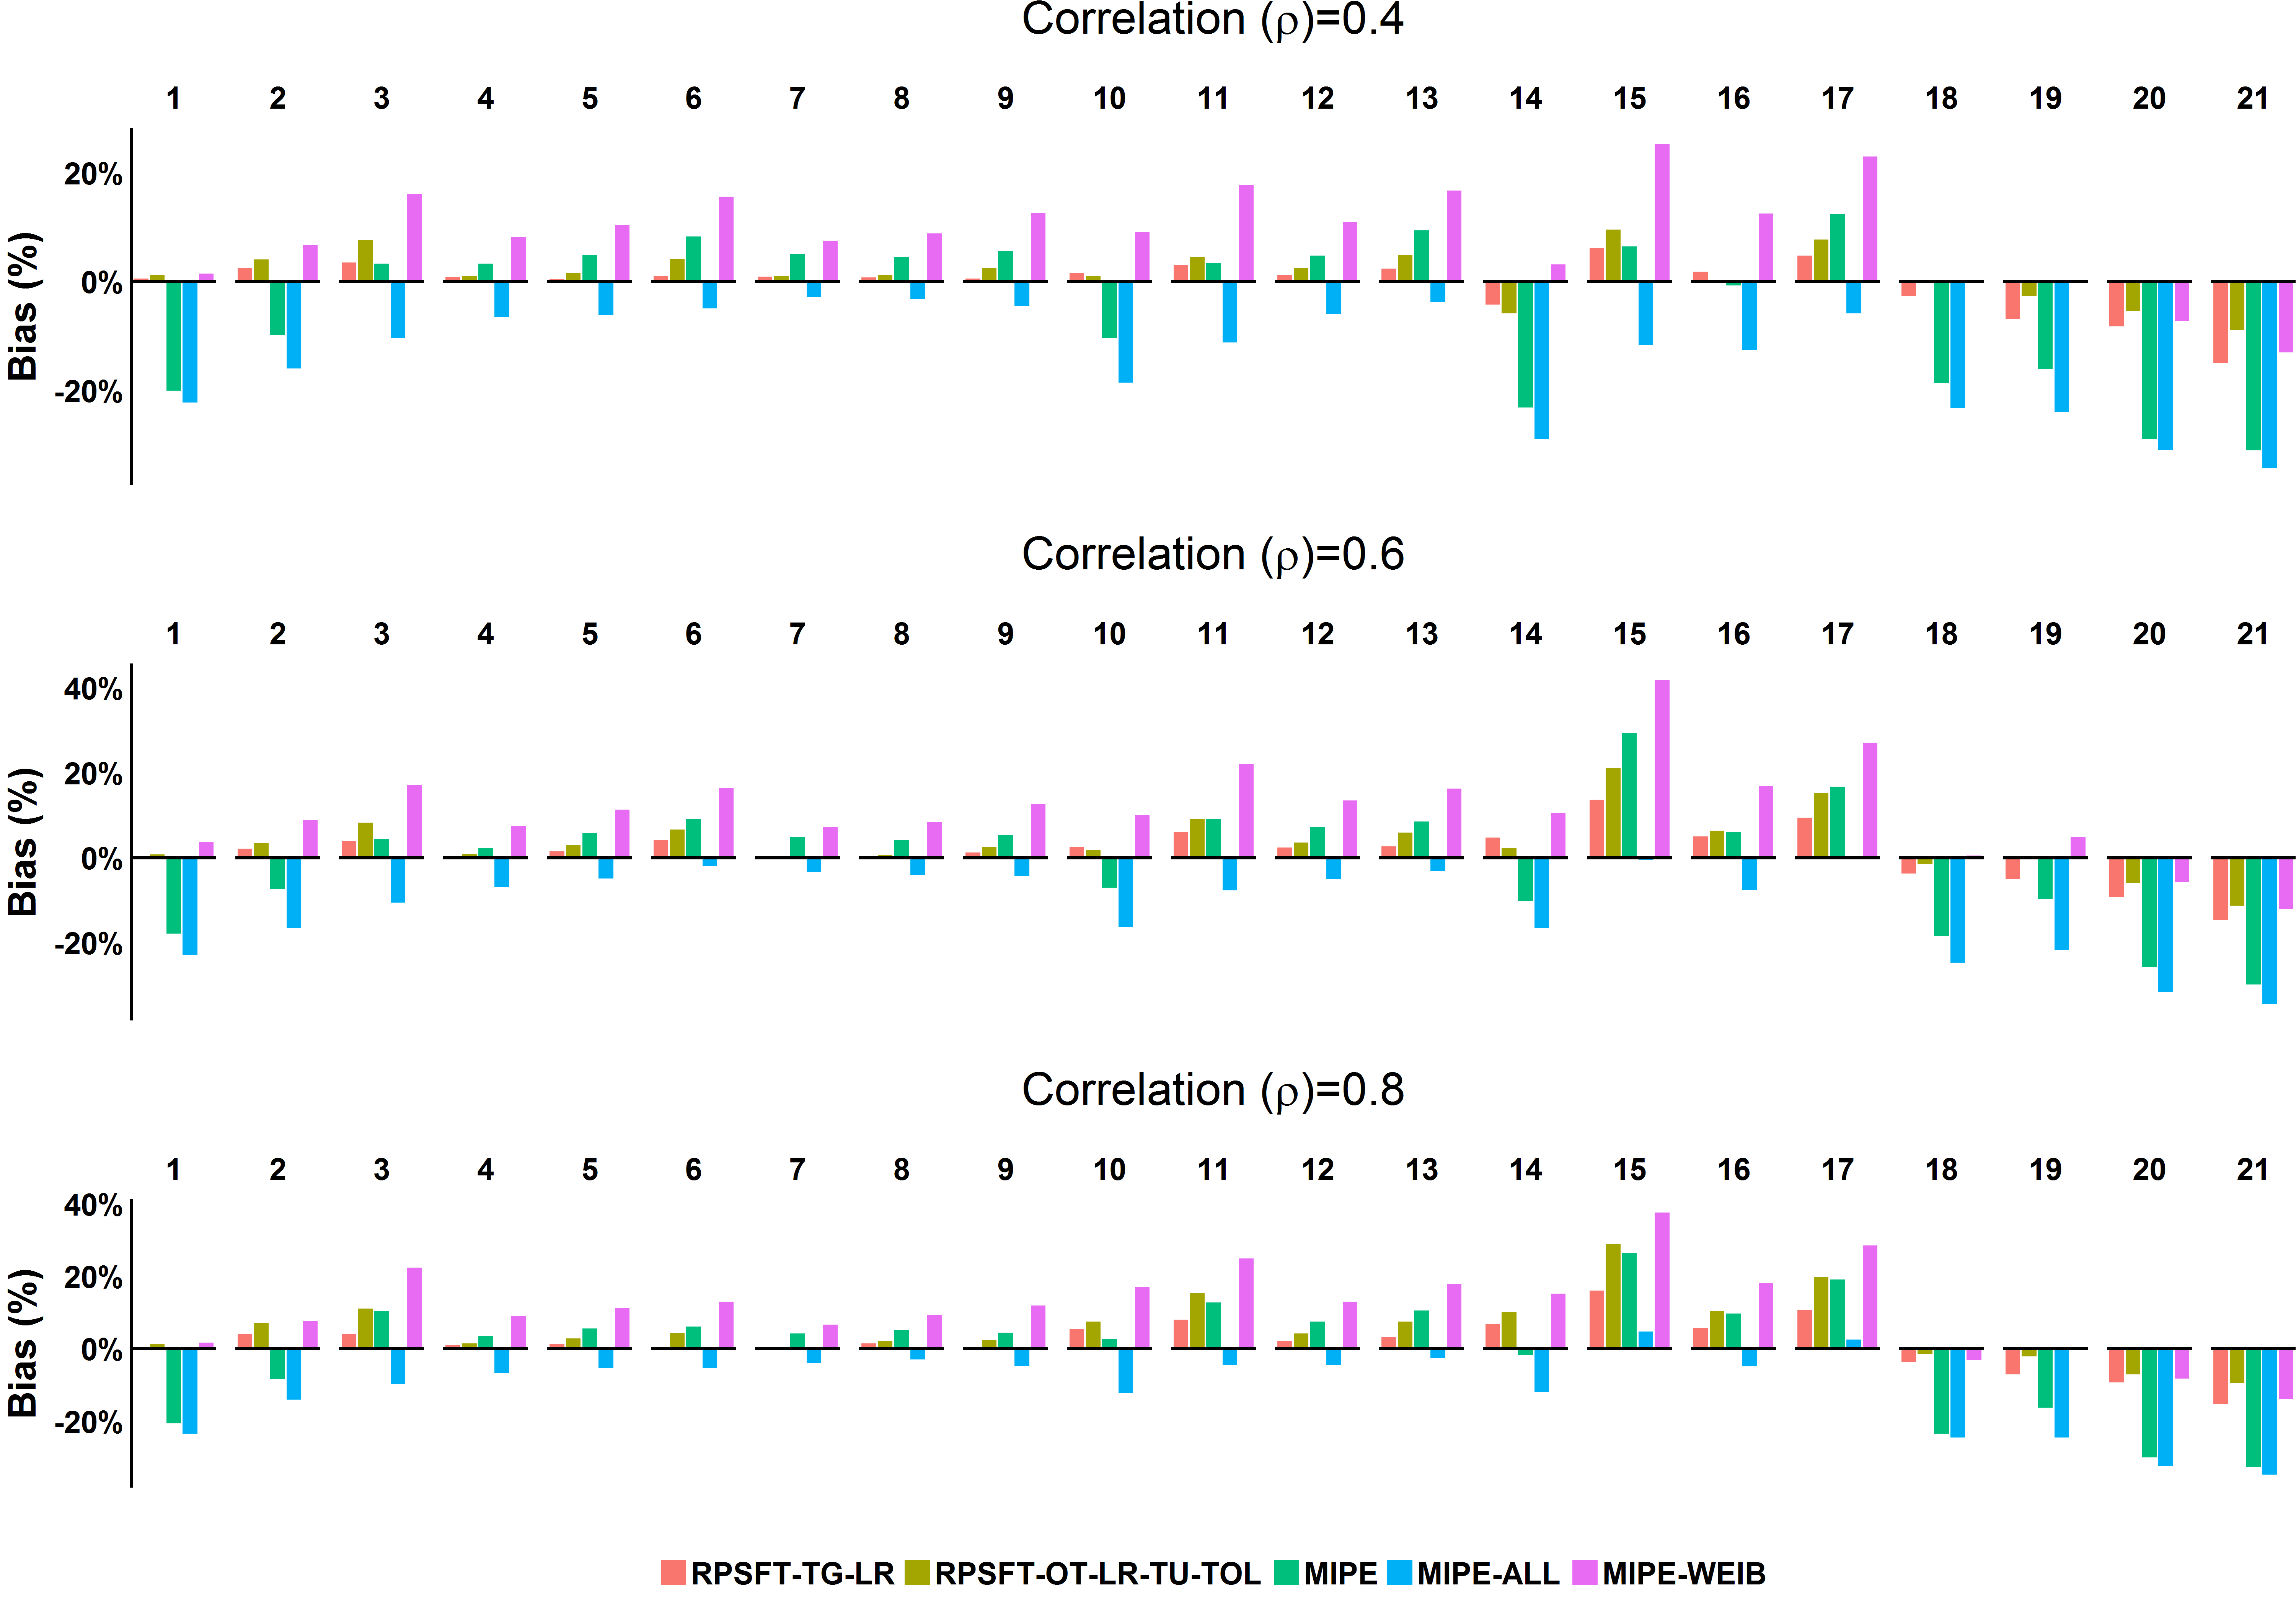
\includegraphics[width=20cm]{images/app_allres/mipe_bias4.png}
    \caption{The percentage bias across all simulations for the MIPE method compared to the RPSFT method. \\ MIPE = modified iterative parameter estimation; MIPE-ALL = imputations for non convergence; MIPE-WEIB = hazard ratio taken from weibull estimation;  TG = ``treatment group''; OT = ``on treatment''; LR = log-rank test}
    \label{F:allp:mipe}
\end{sidewaysfigure}

\begin{sidewaysfigure}
    \centering
    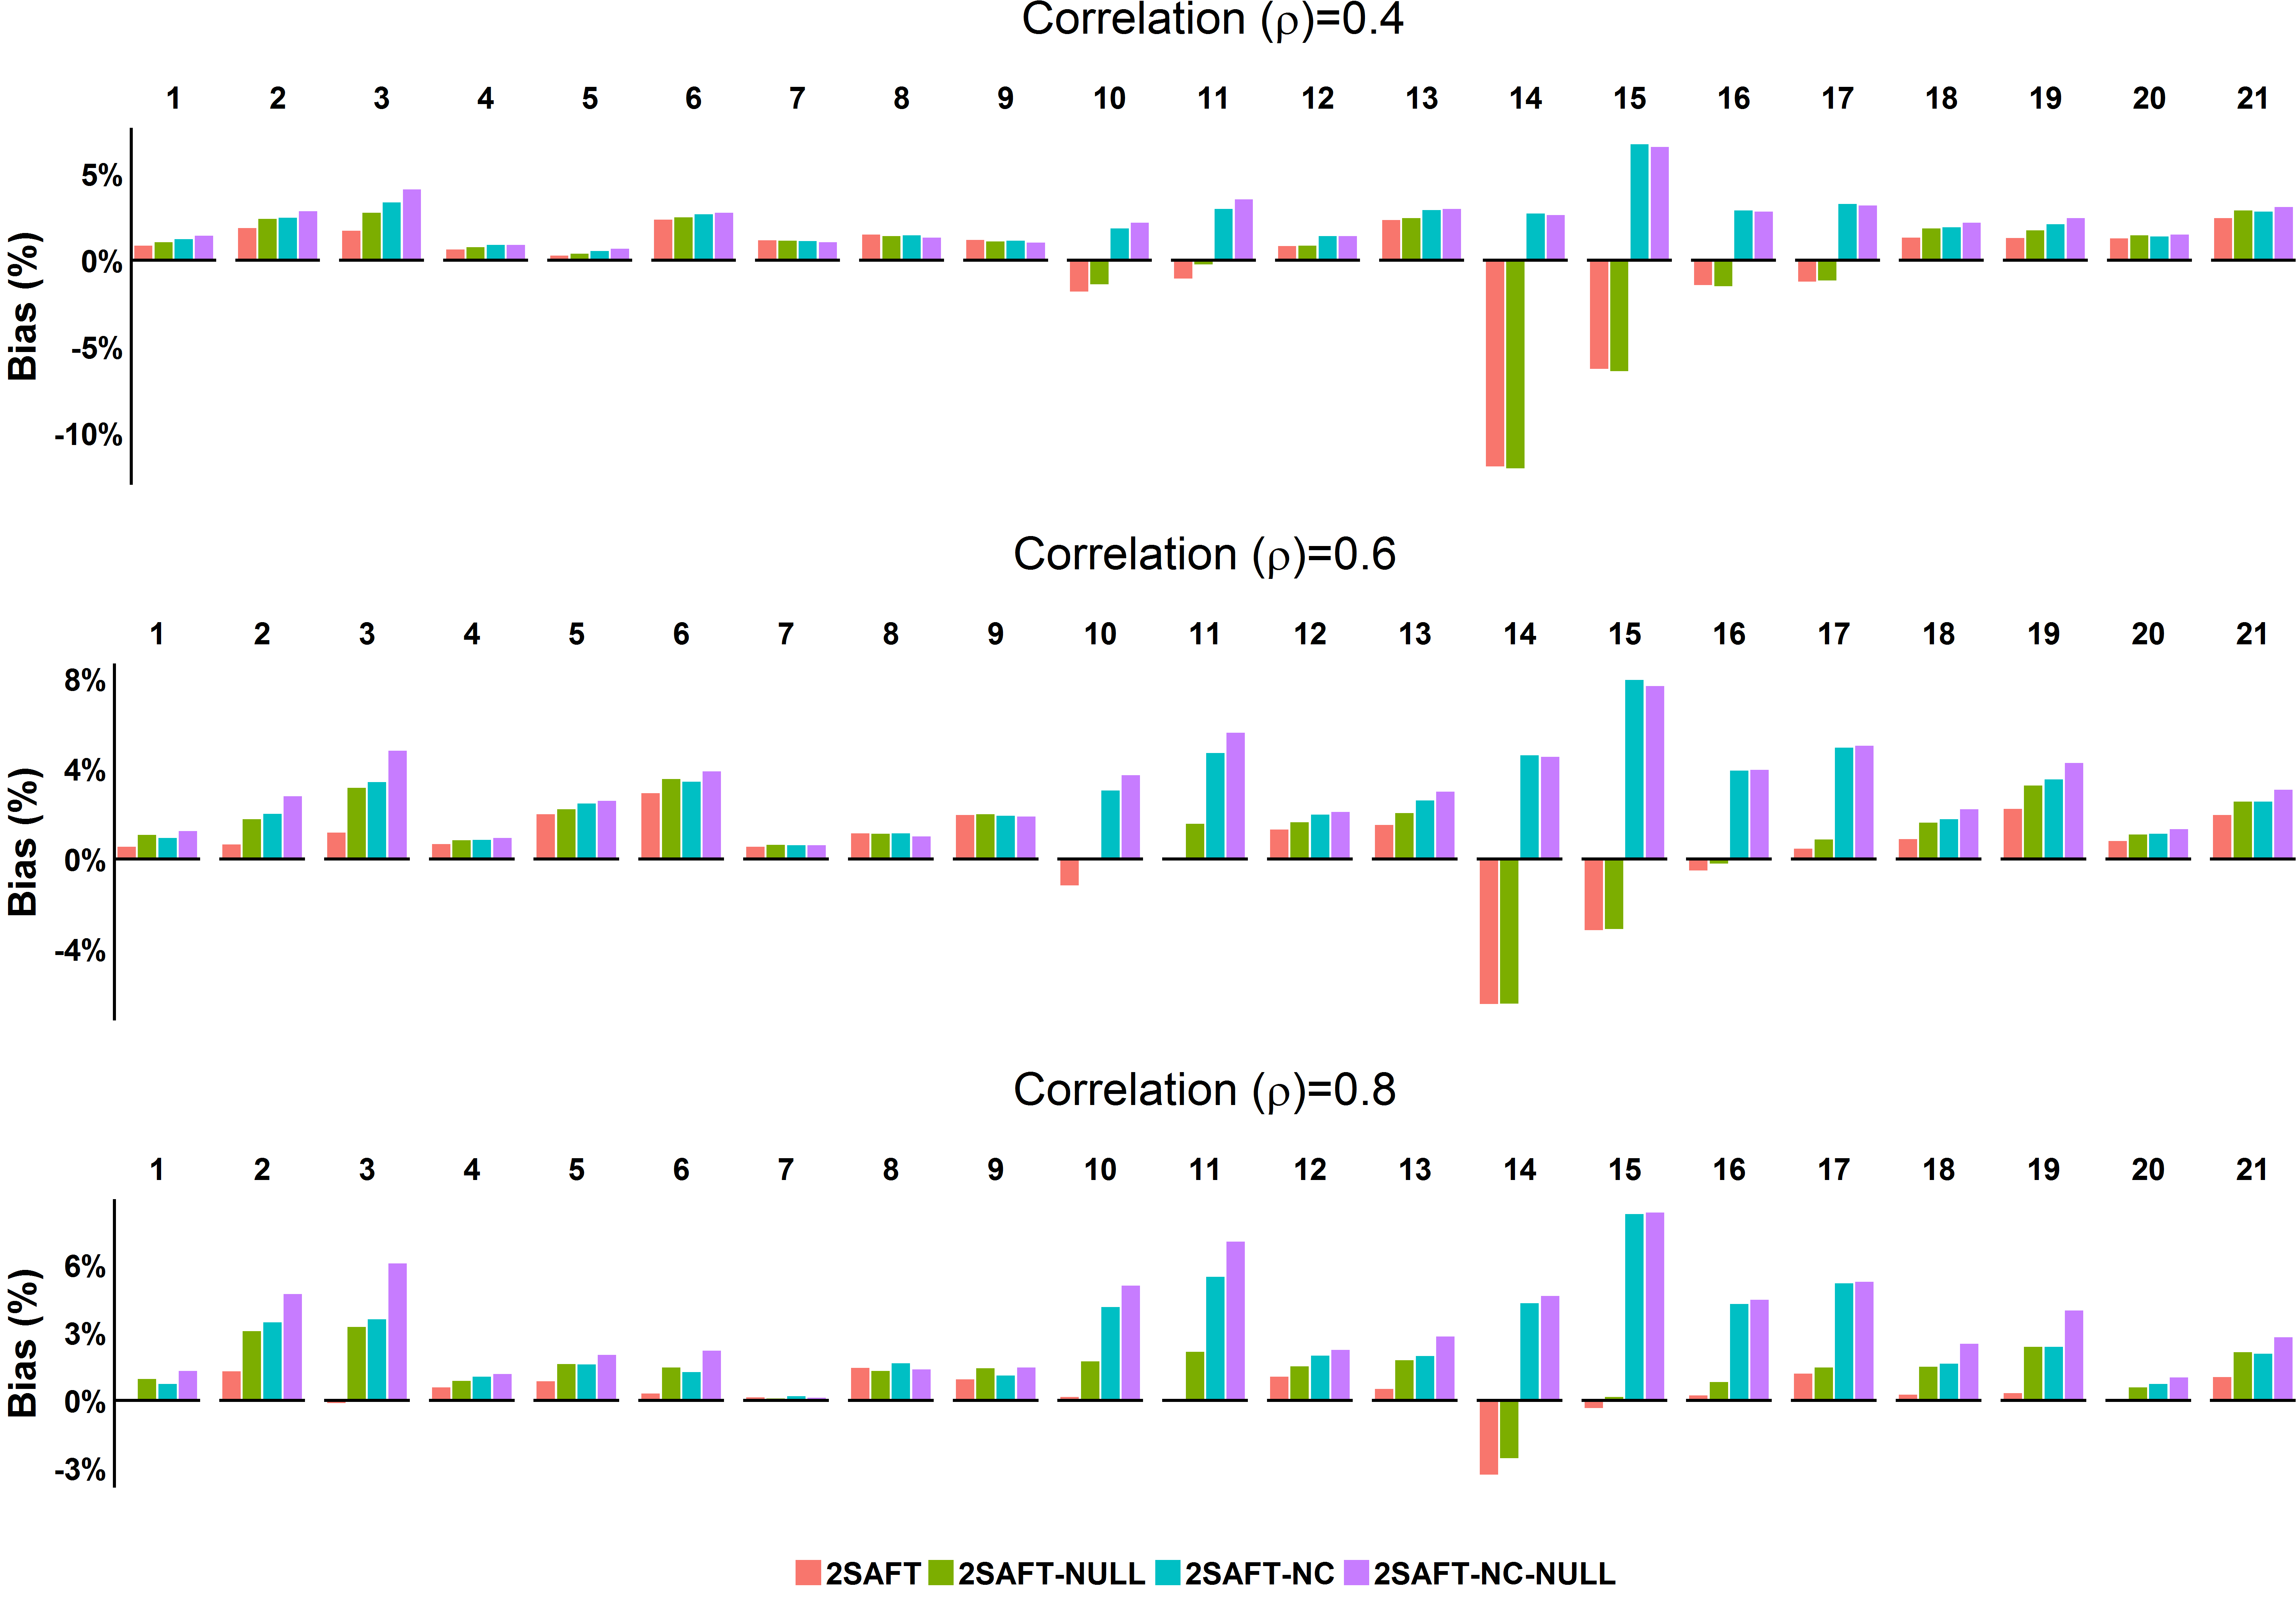
\includegraphics[width=20cm]{images/app_allres/saft_bias4.png}
    \caption{The percentage bias across all simulations for the Two Stage AFT method. \\ 2SAFT = including PFS as a covariate; 2SAFT-NULL = model with no covariates; NC = no recensoring}
    \label{F:allp:saft}
\end{sidewaysfigure}

\chapter{Selected R code}

\label{C:app_R}
This Appendix contains selected R \citep{Rsoftware} code needed to simulate the data used and to apply methods that are not available in standard software.

\section{Methods}
\label{S:app_R:sim1meth}
This section contains the code used to apply the methods described in Chapter \ref{CHAP:methods} that are not available in standard software.
\subsection{Sample data}
The following code creates an example dataset that is used to illustrate the methods here. The function \verb+sim.GenStudy+ can be found in Section \ref{S:app_R:simgen}.
\begin{Verbatim}[fontsize=\small, baselinestretch=0.75]
require(dplyr); require(survival)
exData  <- sim.GenStudy(seed = 1234, rho = 0.4, p.switch = 0.6)
# ITT Hazard Ratio and 95% CI
summary(coxph(Surv(os.t, os.e) ~ x.trt,data = exData))
\end{Verbatim}
\subsection{Rank Preserving Structural Failure Time}
An illustration of estimating a Hazard Ratio and 95\% CI using this method for the ``treatment group'' model with a log-rank test and estimating a hazard ratio using the comparison of $T_i$ and $U_i$ is shown below. Additional functions \verb+RPSFT.2pass+ and \verb+RPSFT.cox+ are defined below. 

\begin{Verbatim}[fontsize=\small, baselinestretch=0.75]
rpsft.input <- transmute(exData, 
                         event.time = os.t,
                         trt.ind    = x.trt, 
                         censor.ind = os.e, 
                         t.start    = ifelse(x.switch|x.trt, 
                                             pmax(0,t.switch,na.rm = TRUE), 
                                             0),
                         t.stop     = ifelse(x.switch|x.trt, 
                                                os.t, 
                                                0),
                         t.on       = t.stop - t.start, 
                         t.off      = os.t - (t.stop - t.start),
                         cutofftime = t.censor)
# do g-estimation
rpsft.output <- RPSFT.2pass(rpsft.input, Grho=0)
# use g-estimation results to calculate CI
summary(RPSFT.cox(rpsft.output, rpsft.input, Grho = 0)$cox.rpsft)
\end{Verbatim}
%dummy for syntax highlight$

\subsubsection{Function RPSFT.2pass}
The function \verb+RPSFT.2pass+ calls function \verb+RPSFT+ twice to perform two grid searches to identify the value of $\psi$ that minimises the chosen test statistic (specified by \verb+Grho+ which defines the test to use from the Harrington and Fleming family so \verb+Grho=0+ is log-rank and \verb+Grho=1+ is Wilcoxon).
\begin{Verbatim}[fontsize=\small, baselinestretch=0.75]
RPSFT.2pass <- 
  function(rpsft.input, 
           pass1.psimat = matrix(ncol = 1, data = 
                                 c(seq(from=-3, to=3, by=0.1))), 
           Grho = 0
){
  # apply RPSFT with wide grid
  pass1 <- RPSFT(rpsft.input, Grho=Grho, psimat = pass1.psimat)  
  
  # get interesting places to look (within 95 percent CI for z)
  pass1.limits <- pass1$psi.tried[abs(pass1$z) <= 1.96]
  pass2.psimat <- matrix(ncol = 1, data = 
          c(seq(from = min(pass1.limits), to = max(pass1.limits), by = 0.01)))  

  # apply RPSFT again
  pass2 <- RPSFT(rpsft.input, Grho=Grho, psimat = pass2.psimat)  

  # combine the grids searched for return
  pass.df <- rbind(data.frame(pass = 1, psi=pass1$psi.tried, z = pass1$z),
                   data.frame(pass = 2, psi=pass2$psi.tried, z = pass2$z))  
  pass.df <- summarise(group_by(pass.df, psi , z), pass = min(pass))  

  # return the second pass but add in the values tried in the first pass
  rc <- pass2
  rc$psi.tried <- pass.df$psi
  rc$z         <- pass.df$z
  rc$pass      <- pass.df$pass 
  return(rc)
}
\end{Verbatim}

\clearpage\newpage
\paragraph{Function RPSFT} performs g-estimation calling functions \verb+RPSFT.trypsi+ and \verb+RPSFT.latent+ repeatedly.

\begin{Verbatim}[fontsize=\small, baselinestretch=0.75]
RPSFT<-function(rpsft.input, psimat, Grho = 0){   
  # derive z values for a range of psi
  z <- apply(psimat,c(1),RPSFT.trypsi, Grho = Grho, rpsft.input = rpsft.input)  
  # chosen value for psi is that which has rank test Z value of 0
  # select based on when sign changes
  x <- sign(z)
  x1 <- x[-1]
  x2 <- x[-length(x)]  
  # selected psi index (either is 0 or is between a sign change)
  indx         <- which(z==0)
  indx_chg_low <- which(x1!= x2 & x1!=0 & x2!=0)
  indx_chg_hgh <- indx_chg_low+1
  psi.found    <- c(psimat[indx,1], 
                    0.5*(psimat[indx_chg_low,1]+psimat[indx_chg_hgh,1])) 
  # is it a unique solution?
  psi.unique <- as.numeric(length(psi.found)==1)  
  # apply proposal of White to take weighted average if is multiple
  psi.chosen <- sum(c(1,rep(c(-1,1),0.5*(length(psi.found)-1)))*psi.found)  
  latent <- RPSFT.latent(psi.chosen, rpsft.input)  
  # return the tested values, associated Z values, chosen psi and latent survival
  rc <- list(psi.tried  = as.numeric(psimat),
             z          = z,
             psi.found  = psi.found,
             psi.unique = psi.unique,
             psi.chosen = psi.chosen,
             latent     = latent
             )
  return(rc)
}
\end{Verbatim}

\paragraph{Function RPSFT.trypsi} estimates $Z(\psi)$ associated with a comparison of counterfactual survival times for a given value of $\psi$.
\begin{Verbatim}[fontsize=\small, baselinestretch=0.75]
RPSFT.trypsi <- function(psi, Grho, rpsft.input){ 
  latent <- RPSFT.latent(psi, rpsft.input)
  sv <- Surv(latent$event.time, latent$censor.ind)
  sd <- survdiff(sv ~ rpsft.input$trt.ind, rho = Grho)
  z  <- sign(sd$obs[2]-sd$exp[2])*sd$chisq^0.5
  return(z)
}
\end{Verbatim}
\paragraph{Function RPSFT.latent} derives latent survival times for a given value of $\psi$ while applying recensoring.
\begin{Verbatim}[fontsize=\small, baselinestretch=0.75]
RPSFT.latent <- function(psi, rpsft.input){
  latent<-data.frame(cstar = pmin(rpsft.input$cutofftime*exp(psi), 
                                  rpsft.input$cutofftime))
  latent$event.time <- pmin(rpsft.input$t.off + rpsft.input$t.on*exp(psi), 
                            latent$cstar )    
  latent$censor.ind <- as.numeric((latent$event.time < latent$cstar) 
                                   & rpsft.input$censor.ind)
  return(latent)
}
\end{Verbatim}
\clearpage\newpage
\subsubsection{Function RPSFT.cox}
The function \verb+RPSFT.cox+ estimates a Hazard Ratio and derives corrected test-based confidence intervals using the methods described in Section \ref{S:chap_methrev:RPSFTestHR}.
\begin{Verbatim}[fontsize=\small, baselinestretch=0.75]
RPSFT.cox <- function(rpsft.output, 
                      rpsft.input, 
                      Grho = 0, 
                      use.latent.only = TRUE
){ 
  # combine the observed and latent times
  df <- cbind(rpsft.input, 
              transmute(rpsft.output$latent, 
                        latent.event.time = event.time, 
                        latent.censor.ind = censor.ind, 
                        psi = rpsft.output$psi.chosen))  
  # derive counterfactual times from latent event times OR as T vs U
  if (use.latent.only){
    df <- mutate(df,
                 lat.on  = pmin(t.on * exp(psi), latent.event.time),
                 lat.off = ifelse((latent.event.time - lat.on) > 0, 
                                  latent.event.time - lat.on, 
                                  0),
                 cfact.time       = ifelse(trt.ind == 1, 
                                           lat.on * exp(-psi) + lat.off,  
                                           latent.event.time ), 
                 cfact.censor.ind = latent.censor.ind
    )
  } else {
    df <- mutate(df, 
                 cfact.time       = ifelse(trt.ind == 1, 
                                           event.time,  
                                           latent.event.time ),
                 cfact.censor.ind = ifelse(trt.ind == 1, 
                                           censor.ind,  
                                           latent.censor.ind )
    )                 
  }  
  # derive corrected hazard ratios
  cox.rpsft <- coxph(Surv(cfact.time, cfact.censor.ind) ~ trt.ind, data = df)  
  # correct standard error using Z value
  cox.rpsft$var.orig <- cox.rpsft$var
  z0 <- survdiff(Surv(event.time, censor.ind) ~ trt.ind, 
                 data = df, 
                 rho = Grho)$chisq ^ 0.5
  cox.rpsft$var <- matrix((abs(coef(cox.rpsft)) / z0)^2)  
  rc <- list(cox.rpsft = cox.rpsft, 
             cfact.time = df$cfact.time, 
             cfact.censor.ind = df$cfact.censor.ind, 
             psi.unique = rpsft.output$psi.unique)  
  return(rc)  
}
\end{Verbatim}
%dummy - correct highlight $
\clearpage
\newpage

\section{Code to Simulate data}
\label{S:app_R:simgen}
The function \verb+sim.GenStudy+ generates data as described in Chapter \ref{C:chap_sim_design}.

\begin{Verbatim}[fontsize=\small, baselinestretch=0.75]

sim.GenStudy <- function(
  # params modified by sim 
  simid         , # identifier
  seed          , # seed
  rho           , # correlation coefficient between switch time and os
  p.switch      , # proportion switch 
  prop.pd.int   , # proportion of patients with PFS before switch allowed
  beta_1a       , # treatment effect (as log(Hazard Ratio))
  beta_1b       , # treatment effect (as log(Hazard Ratio))
  beta_2a       , # treatment effect (as log(Hazard Ratio))
  beta_2b       , # treatment effect (as log(Hazard Ratio))
  # params not changed across all sims
  beta_pd       = log(0.4),  # treatment effect on TTP (as log(HR))  
  arm.n         = 250,       # patients per arm
  enroll.start  = 0,         # start of enrollment
  enroll.end    = 2,         # end of enrollment
  admin.censor  = 3,         # end of trial
  os.gamma      = 1.2,       # weibull shape - for OS
  os.lambda     = 0.3,       # weibull scale - for OS
  ttp.gamma     = 1.5,       # weibull shape - for TTP
  ttp.lambda    = 2          # weibull scale - for TTP
){
  set.seed(seed)  
  # combine so can select based on x 
  n_switch <- arm.n * p.switch  
  # u1 is just used to setup then not used
  # u2 and u3 are correlated uniform random variables used for OS and switch time
  # u4 used for censoring time (entry time)
  # u5 used for selecting switchers
  u <- matrix(nrow = arm.n*2, ncol = 5,data = runif(arm.n*2*5,0,1))
  # setup correlations using normal variables then convert back to uniform
  u[,3] <- pnorm(rho* qnorm(u[,2],0,1) + ((1-rho^2)^0.5)*qnorm(u[,1],0,1),0,1)  
  # generate covariates
  x.trt    <- rep(c(0,1), each = arm.n)  
  # generate os without treatment
  os.basis.t  <- (-(log(u[,2]) / (os.lambda)))^(1/os.gamma)  
  # generate ttp 
  ttp.untreated.t <- (-(log(u[,3]) / (ttp.lambda)))^(1/ttp.gamma)  
  # apply treatment effect
  ttp.treated.t <-(-(log(u[,3]) / (ttp.lambda*exp(beta_pd))))^(1/ttp.gamma)  
  # deive basis ttp
  ttp.basis.t <- ifelse(x.trt==1, ttp.treated.t, ttp.untreated.t)
  # generate pfs
  pfs.basis.t <- pmin(os.basis.t, ttp.basis.t)
  # generate entry time
  t.entry <- enroll.start + runif(u[,4])*(enroll.end-enroll.start)
  # generate follow up time
  t.censor <- admin.censor - t.entry
  # define a time in trial after which switch happens
  t.start.switch <- as.numeric(quantile(t.entry + pfs.basis.t, prop.pd.int))
  # who can switch - have ttp before os and censor
  can.switch <- as.numeric(
    ttp.basis.t < os.basis.t &
      ttp.basis.t < t.censor &
        t.entry+ttp.basis.t >= t.start.switch
  )[x.trt==0]  
  rank <- rep(arm.n,arm.n)
  # choose randomly from those who can switch to get the
  # required  number of switchers
  rank[can.switch==1] <- order(u[x.trt==0 & can.switch==1,5])
  x.switch <- c(as.numeric(rank<=n_switch), rep(0,arm.n))
  # calculate how many actually switch 
  actual.p.switch <- sum(x.switch) / arm.n
  # generate switch time
  t.switch <- rep(NA,arm.n*2)
  t.switch[x.switch==1] <- ttp.basis.t[x.switch==1]
  
  # get control non switch os
  os.orig.t <- rep(NA,arm.n*2)
  os.orig.t[x.trt == 0] <- (-(log(u[x.trt==0,2])) / (os.lambda ))^(1/os.gamma)
  
  # get experimental arm os
  t0  <- ttp.basis.t 
  t0v <- t0 ^ os.gamma
  c1 <- os.lambda * exp(beta_1a)
  c2 <- os.lambda * exp(beta_1b)
  v1 <- 1/os.gamma
  os.orig.t[x.trt == 1] <- ifelse(-log(u[x.trt==1,2])  < c1 * t0v[x.trt==1],
                                 (-log(u[x.trt==1,2]) / c1) ^ v1,
                                 ((-log(u[x.trt==1,2]) -
                                      c1*t0v[x.trt==1] + 
                                      c2*t0v[x.trt==1]) / c2) ^ v1
                                  )

  # get switch treatment (start from orig)
  os.cross.t <- os.orig.t
  t1 <- ttp.basis.t
  t2 <- ttp.basis.t + ttp.treated.t
  t1v <- t1^os.gamma
  t2v <- t2^os.gamma
  c3 <- os.lambda*exp(beta_2a)
  c4 <- os.lambda*exp(beta_2b)
  d1 <- x.switch==1 & -log(u[,2]) < os.lambda*t1v
  d3 <- x.switch==1 & -log(u[,2]) >= os.lambda*t1v + c3*(t2-t1)
  d2 <- x.switch==1 & -log(u[,2]) >= os.lambda*t1v & !d3
  os.cross.t[d1] <- (-log(u[d1,2]) / os.lambda )^v1
  os.cross.t[d2] <- ((-log(u[d2,2])- os.lambda*t1v[d2] + 
                      c3*t1v[d2]) / c3 )^v1
  os.cross.t[d3] <- ((-log(u[d3,2]) -
                      os.lambda*t1v[d3] - 
                      c3*(t2v[d3] - 
                      t1v[d3]) +c4*t2v[d3]) / c4 )^v1
  
  # apply censoring
  os.b.t <- pmin(os.basis.t, t.censor)
  os.b.c <- as.numeric(os.b.t==t.censor)
  os.o.t <- pmin(os.orig.t, t.censor)
  os.o.c <- as.numeric(os.o.t==t.censor)
  os.t <- pmin(os.cross.t, t.censor)
  os.c <- as.numeric(os.t==t.censor)
  # store ttp 
  ttp.t <- pmin(ttp.basis.t, t.censor)
  ttp.c <- as.numeric(ttp.t==t.censor)
  # derive PFS (min of os and ttp) 
  pfs.t <- pmin(os.t, ttp.t)
  pfs.c <- as.numeric(pfs.t==t.censor)
  # create a data frame
  patid <- 1:(arm.n*2)  
  df <- data.frame(patid    = patid,
                   x.trt    = x.trt,
                   x.switch = x.switch,
                   t.switch = t.switch,
                   t.censor = t.censor,
                   ttp.t    = ttp.t,
                   ttp.e    = 1 - ttp.c,
                   pfs.t    = pfs.t,
                   pfs.e    = 1 - pfs.c,
                   os.b.t   = os.b.t,
                   os.b.t   = 1 - os.b.c,
                   os.t     = os.t,
                   os.e     = 1 - os.c,
                   os.o.t   = os.o.t,
                   os.o.e   = 1 - os.o.c,
                   seed     = seed,
                   rho      = rho,
                   prop.pd.int = prop.pd.int,
                   p.switch = p.switch,
                   beta_1a = beta_1a,
                   beta_1b = beta_1b,
                   beta_2a = beta_2a,
                   beta_2b = beta_2b,
                   simid   = simid,
                   actual.p.switch = actual.p.switch
  )
  return(df)
}
\end{Verbatim}
\include{app_genweib}
\chapter{Additional results of Simulation Study 1}

\label{A:sim2res}

This Appendix contains additional results for the simulation study described in Chapter \ref{C:chap_sim2}. Figure \ref{F:app_sim2:compA_bias} shows the bias and Figure \ref{F:app_sim2:compA_cov} the coverage of each of the complex methods after the imputations discussed in Section \ref{S:chap_sim2:convimp} were applied. Overall the results are similar to that seen without these imputations. 

\begin{figure}[ht]
\centering
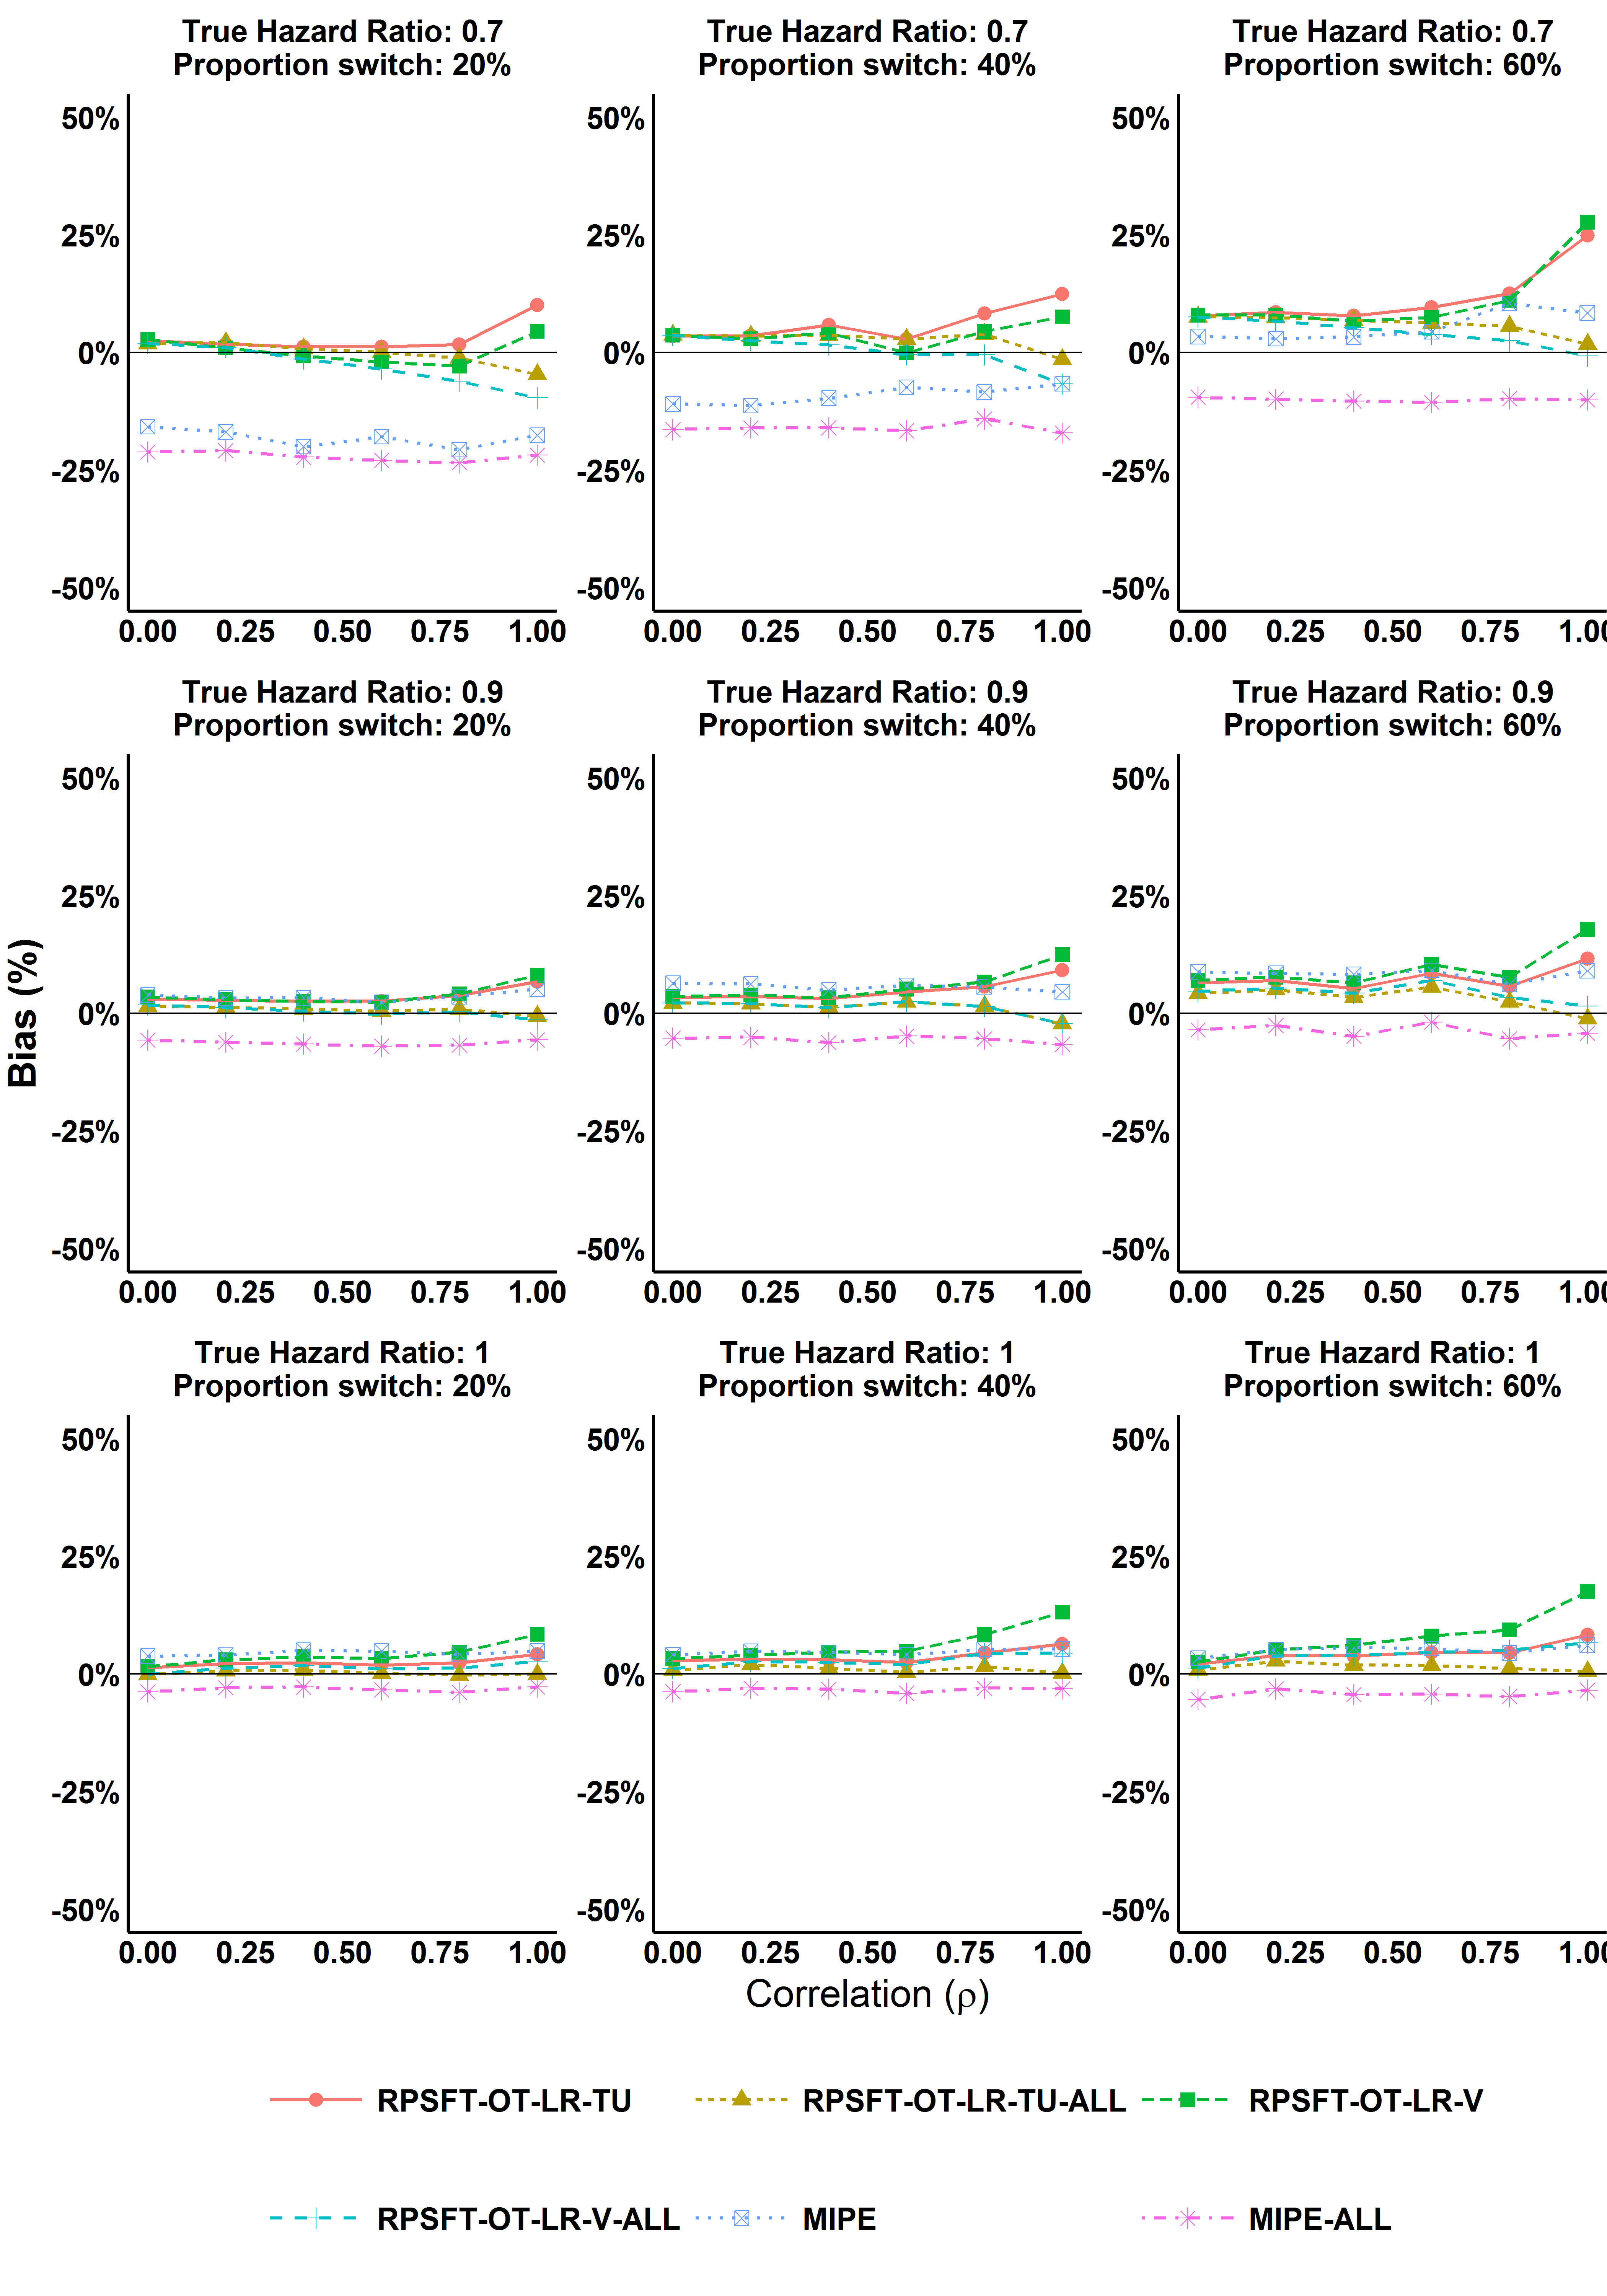
\includegraphics[width=14cm]{images/app_sim2res/complexA_bias.png}
\caption{\label{F:app_sim2:compA_bias} The bias for each of the complex methods across all the scenarios when imputations are made to address non-convergence. The results are very similar to what is seen when non-converging simulations were excluded.} 
\end{figure}

\begin{figure}[ht]
\centering
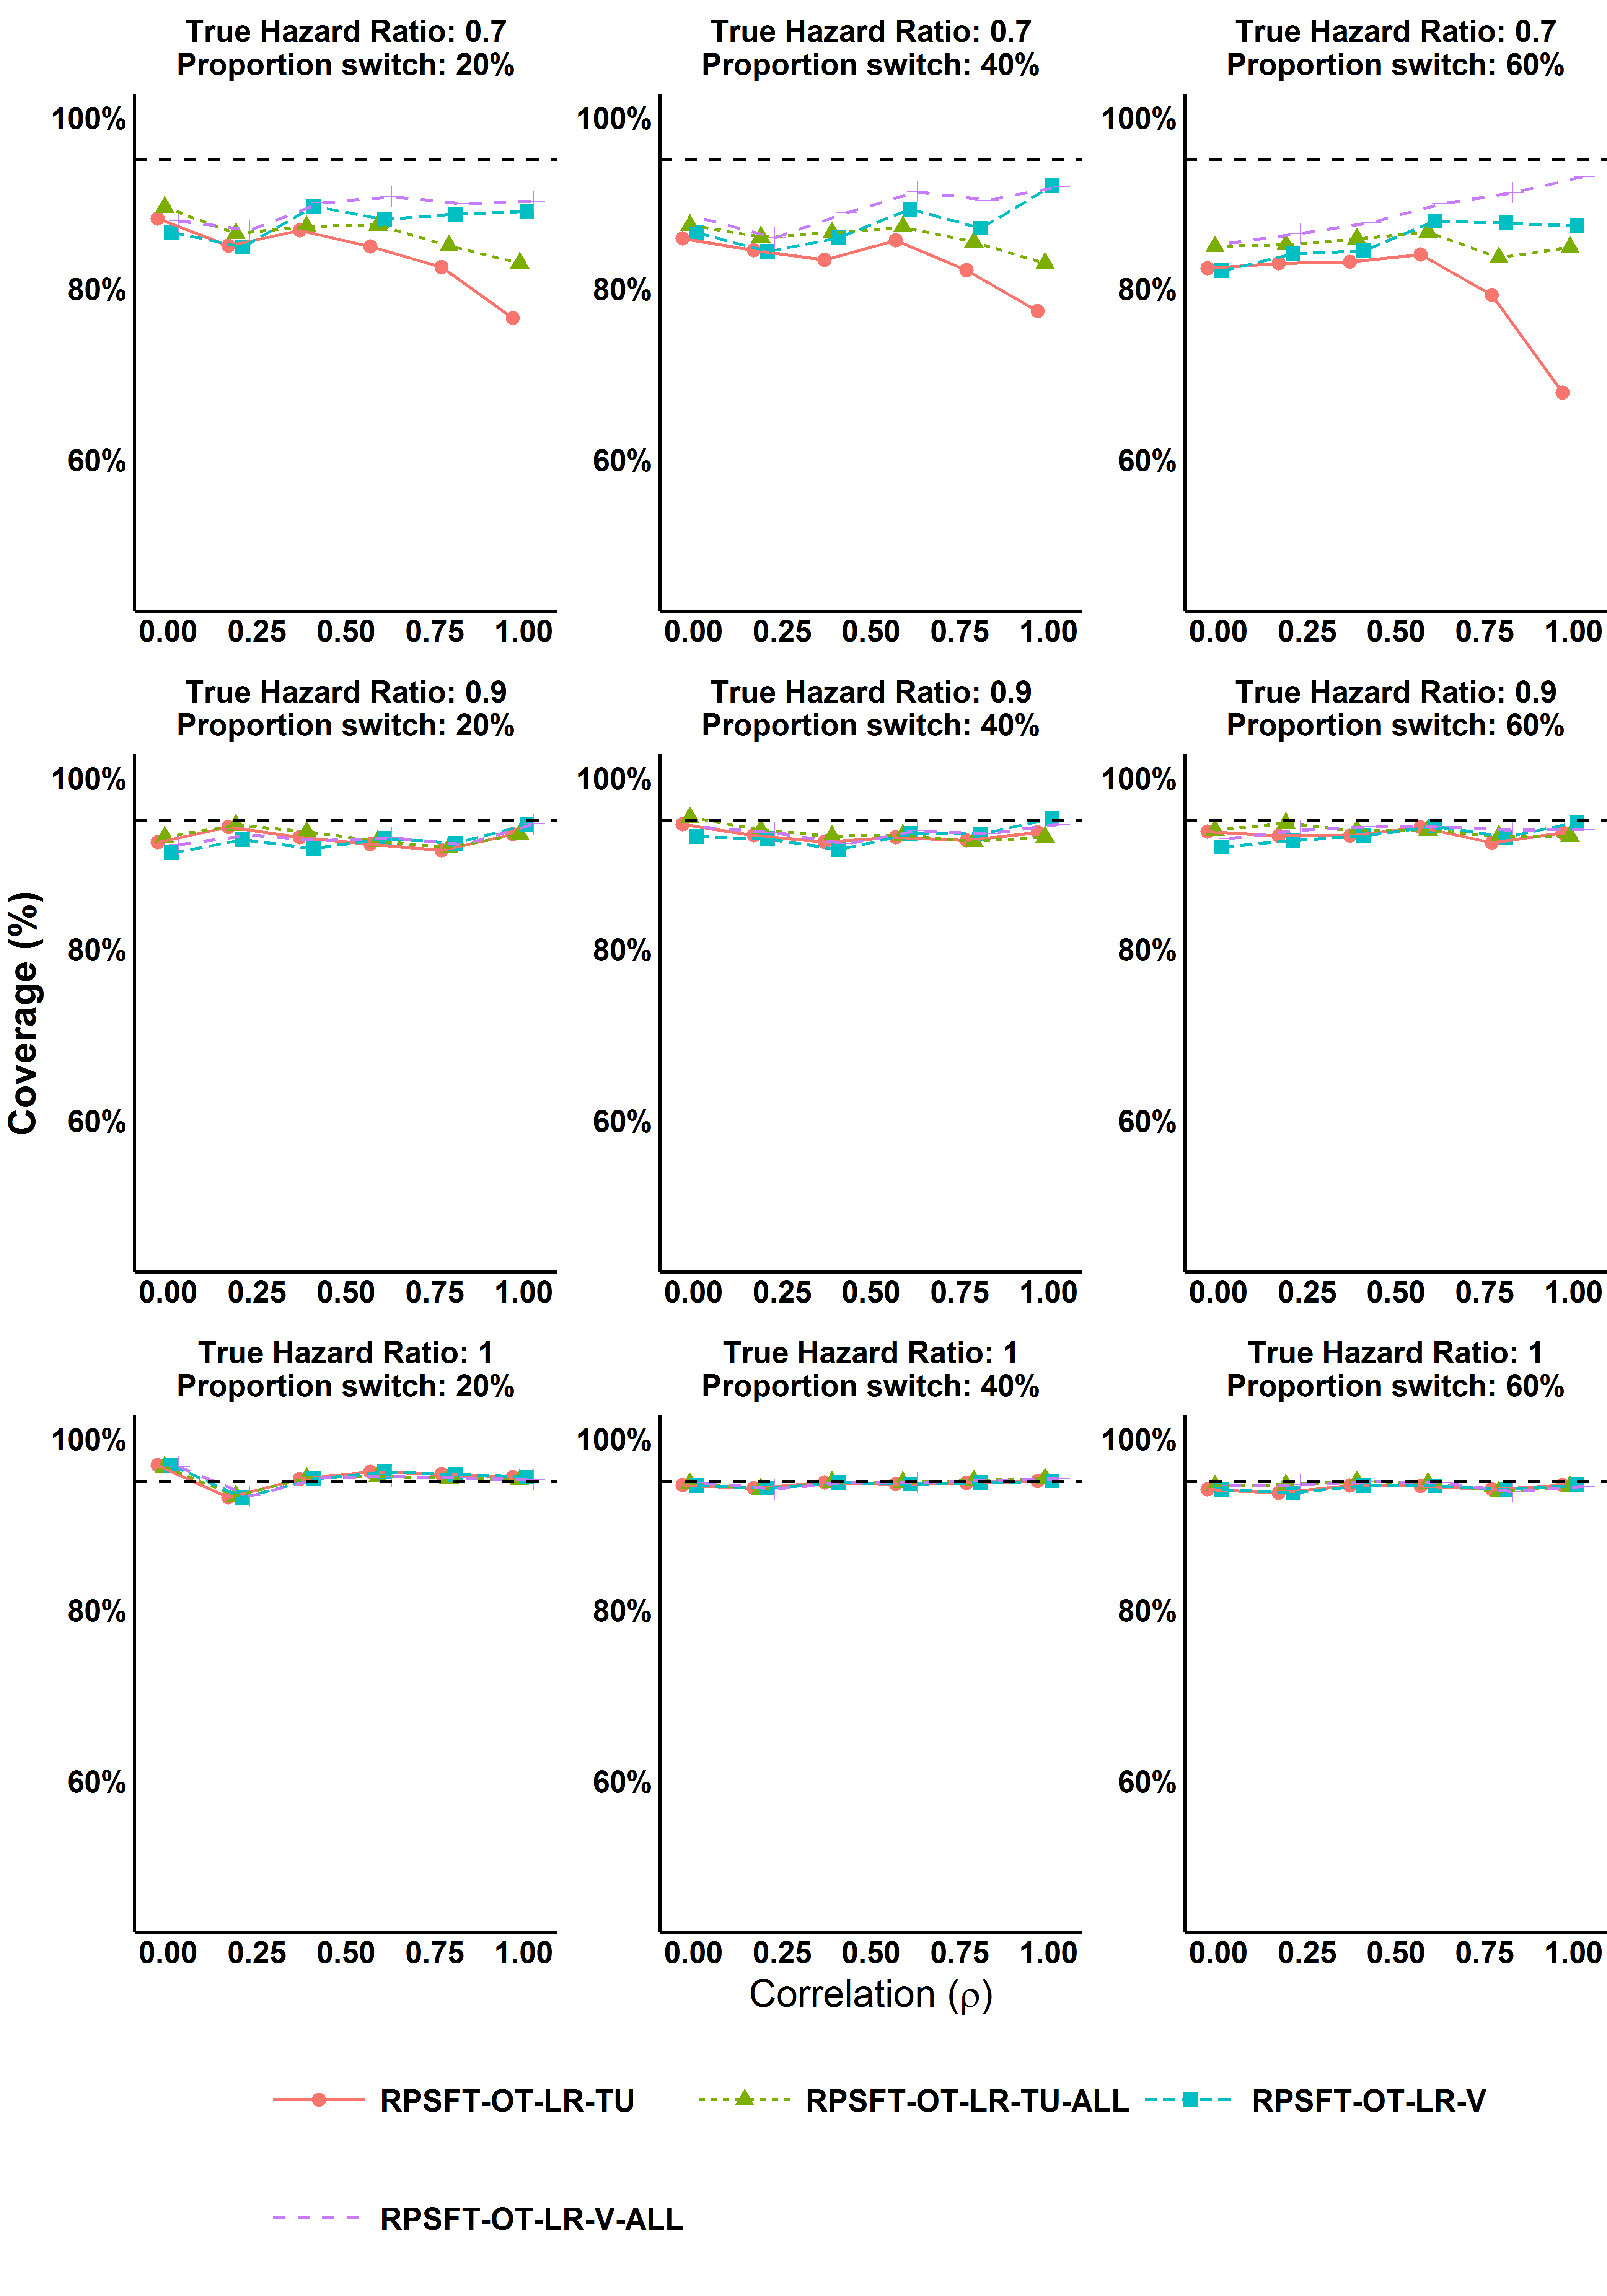
\includegraphics[width=14cm]{images/app_sim2res/complexA_cov.png}
\caption{\label{F:app_sim2:compA_cov} The coverage for each of the complex methods across all the scenarios when imputations are made to address non-convergence. The results are very similar to what is seen when non-converging simulations were excluded.} 
\end{figure}

\clearpage

\section{Complete results for Simulation Study 1}
\large\textbf{Contents}\\


% latex table generated in R 3.3.1 by xtable 1.8-2 package
% Thu Sep 15 18:20:50 2016
\begingroup\small
\begin{tabular}{ll}
  \hline
\hline
Table & Title \\ 
  \hline
Table \ref{T:app.sim2.res.1} & Results for study 1 with true HR $\exp(\beta_{1a}) =0.7$ and correlation $\rho =0$ \\ 
  Table \ref{T:app.sim2.res.2} & Results for study 1 with true HR $\exp(\beta_{1a}) =0.7$ and correlation $\rho =0.2$ \\ 
  Table \ref{T:app.sim2.res.3} & Results for study 1 with true HR $\exp(\beta_{1a}) =0.7$ and correlation $\rho =0.4$ \\ 
  Table \ref{T:app.sim2.res.4} & Results for study 1 with true HR $\exp(\beta_{1a}) =0.7$ and correlation $\rho =0.6$ \\ 
  Table \ref{T:app.sim2.res.5} & Results for study 1 with true HR $\exp(\beta_{1a}) =0.7$ and correlation $\rho =0.8$ \\ 
  Table \ref{T:app.sim2.res.6} & Results for study 1 with true HR $\exp(\beta_{1a}) =0.7$ and correlation $\rho =1$ \\ 
   \hline
Table \ref{T:app.sim2.res.7} & Results for study 1 with true HR $\exp(\beta_{1a}) =0.9$ and correlation $\rho =0$ \\ 
  Table \ref{T:app.sim2.res.8} & Results for study 1 with true HR $\exp(\beta_{1a}) =0.9$ and correlation $\rho =0.2$ \\ 
  Table \ref{T:app.sim2.res.9} & Results for study 1 with true HR $\exp(\beta_{1a}) =0.9$ and correlation $\rho =0.4$ \\ 
  Table \ref{T:app.sim2.res.10} & Results for study 1 with true HR $\exp(\beta_{1a}) =0.9$ and correlation $\rho =0.6$ \\ 
  Table \ref{T:app.sim2.res.11} & Results for study 1 with true HR $\exp(\beta_{1a}) =0.9$ and correlation $\rho =0.8$ \\ 
  Table \ref{T:app.sim2.res.12} & Results for study 1 with true HR $\exp(\beta_{1a}) =0.9$ and correlation $\rho =1$ \\ 
   \hline
Table \ref{T:app.sim2.res.13} & Results for study 1 with true HR $\exp(\beta_{1a}) =1$ and correlation $\rho =0$ \\ 
  Table \ref{T:app.sim2.res.14} & Results for study 1 with true HR $\exp(\beta_{1a}) =1$ and correlation $\rho =0.2$ \\ 
  Table \ref{T:app.sim2.res.15} & Results for study 1 with true HR $\exp(\beta_{1a}) =1$ and correlation $\rho =0.4$ \\ 
  Table \ref{T:app.sim2.res.16} & Results for study 1 with true HR $\exp(\beta_{1a}) =1$ and correlation $\rho =0.6$ \\ 
  Table \ref{T:app.sim2.res.17} & Results for study 1 with true HR $\exp(\beta_{1a}) =1$ and correlation $\rho =0.8$ \\ 
  Table \ref{T:app.sim2.res.18} & Results for study 1 with true HR $\exp(\beta_{1a}) =1$ and correlation $\rho =1$ \\ 
   \hline
\end{tabular}
\endgroup


%the rest of the tables
% latex table generated in R 3.3.1 by xtable 1.8-2 package
% Thu Sep 15 18:20:50 2016
\begin{table}[ht]
\centering
\caption{Simulation Study 1 Results with True HR =0.7, $\rho =0$ \label{T:app.sim2.res.1}} 
\scalebox{0.6}{
\begin{tabular}{llrrrrr}
  \hline
\hline
Switch  & Method & Mean Est. & Bias & MSE &  Coverage  & Convergence \\ $(\%)$ & & $\exp(\hat{\beta})$ &  (\%) & & $(\%)$ & $(\%)$ \\ 
  \hline
20\% & ITT & 0.75 & 7.18 & 0.01 & 92.1 & 100.0 \\ 
  20\% & PP-CENS & 0.71 & 1.46 & 0.01 & 93.8 & 100.0 \\ 
  20\% & PP-EX & 0.66 & -5.32 & 0.01 & 93.0 & 100.0 \\ 
  20\% & TVC & 0.71 & 1.40 & 0.01 & 94.1 & 100.0 \\ 
  20\% & TVC2 & 0.71 & 1.44 & 0.01 & 93.8 & 100.0 \\ 
   \hline
20\% & RPSFT-TG-LR & 0.71 & 1.55 & 0.02 & 92.0 & 99.9 \\ 
  20\% & RPSFT-TG-LR-ALL & 0.71 & 1.60 & 0.02 & 92.0 & 100.0 \\ 
  20\% & RPSFT-TG-W & 0.71 & 1.45 & 0.02 & 92.2 & 100.0 \\ 
  20\% & RPSFT-TG-W-ALL & 0.71 & 1.45 & 0.02 & 92.2 & 100.0 \\ 
  20\% & RPSFT-OT-LR-TU & 0.72 & 2.55 & 0.02 & 88.1 & 75.9 \\ 
  20\% & RPSFT-OT-LR-TU-ALL & 0.71 & 1.90 & 0.02 & 89.5 & 100.0 \\ 
  20\% & RPSFT-OT-LR-V & 0.72 & 2.76 & 0.02 & 86.6 & 75.9 \\ 
  20\% & RPSFT-OT-LR-V-ALL & 0.71 & 1.95 & 0.02 & 87.9 & 100.0 \\ 
   \hline
20\% & RPSFT-OT-W-TU & 0.72 & 2.35 & 0.02 & 90.5 & 75.9 \\ 
  20\% & RPSFT-OT-W-TU-ALL & 0.71 & 1.90 & 0.02 & 91.0 & 100.0 \\ 
  20\% & RPSFT-OT-W-V & 0.72 & 2.46 & 0.02 & 89.6 & 75.9 \\ 
  20\% & RPSFT-OT-W-V-ALL & 0.71 & 1.89 & 0.02 & 90.3 & 100.0 \\ 
   \hline
20\% & 2SAFT & 0.71 & 1.38 & 0.01 & 93.6 & 100.0 \\ 
  20\% & 2SAFT-NULL & 0.71 & 1.43 & 0.01 & 94.0 & 100.0 \\ 
  20\% & 2SAFT-NC & 0.71 & 1.50 & 0.01 & 92.5 & 100.0 \\ 
  20\% & 2SAFT-NC-NULL & 0.71 & 1.47 & 0.01 & 92.5 & 100.0 \\ 
  20\% & MIPE & 0.59 & -15.77 & 0.05 & 44.8 & 29.0 \\ 
  20\% & MIPE-ALL & 0.55 & -21.15 & 0.05 & 47.2 & 100.0 \\ 
  20\% & MIPE-WEIB & 0.73 & 4.91 & 0.02 &  & 29.0 \\ 
   \hline
40\% & ITT & 0.79 & 13.00 & 0.02 & 87.8 & 100.0 \\ 
  40\% & PP-CENS & 0.70 & 0.64 & 0.01 & 94.8 & 100.0 \\ 
  40\% & PP-EX & 0.59 & -16.12 & 0.02 & 75.0 & 100.0 \\ 
  40\% & TVC & 0.70 & 0.40 & 0.01 & 94.9 & 100.0 \\ 
  40\% & TVC2 & 0.70 & 0.63 & 0.01 & 95.0 & 100.0 \\ 
   \hline
40\% & RPSFT-TG-LR & 0.72 & 2.55 & 0.02 & 92.5 & 99.8 \\ 
  40\% & RPSFT-TG-LR-ALL & 0.72 & 2.64 & 0.02 & 92.5 & 100.0 \\ 
  40\% & RPSFT-TG-W & 0.71 & 2.13 & 0.02 & 92.3 & 99.6 \\ 
  40\% & RPSFT-TG-W-ALL & 0.72 & 2.32 & 0.02 & 92.2 & 100.0 \\ 
  40\% & RPSFT-OT-LR-TU & 0.72 & 3.52 & 0.03 & 85.8 & 73.4 \\ 
  40\% & RPSFT-OT-LR-TU-ALL & 0.73 & 3.77 & 0.02 & 87.4 & 100.0 \\ 
  40\% & RPSFT-OT-LR-V & 0.73 & 3.67 & 0.03 & 86.5 & 73.4 \\ 
  40\% & RPSFT-OT-LR-V-ALL & 0.73 & 3.67 & 0.02 & 88.1 & 100.0 \\ 
   \hline
40\% & RPSFT-OT-W-TU & 0.72 & 3.31 & 0.03 & 88.1 & 73.4 \\ 
  40\% & RPSFT-OT-W-TU-ALL & 0.73 & 3.80 & 0.02 & 89.2 & 100.0 \\ 
  40\% & RPSFT-OT-W-V & 0.72 & 3.43 & 0.03 & 87.7 & 73.4 \\ 
  40\% & RPSFT-OT-W-V-ALL & 0.73 & 3.69 & 0.02 & 89.2 & 100.0 \\ 
   \hline
40\% & 2SAFT & 0.71 & 1.15 & 0.02 & 92.9 & 100.0 \\ 
  40\% & 2SAFT-NULL & 0.71 & 1.11 & 0.02 & 93.0 & 100.0 \\ 
  40\% & 2SAFT-NC & 0.70 & 0.71 & 0.01 & 93.0 & 100.0 \\ 
  40\% & 2SAFT-NC-NULL & 0.70 & 0.68 & 0.01 & 93.1 & 100.0 \\ 
  40\% & MIPE & 0.62 & -10.93 & 0.06 & 44.2 & 31.2 \\ 
  40\% & MIPE-ALL & 0.59 & -16.38 & 0.05 & 51.6 & 100.0 \\ 
  40\% & MIPE-WEIB & 0.74 & 6.23 & 0.04 &  & 31.2 \\ 
   \hline
60\% & ITT & 0.84 & 19.81 & 0.03 & 77.7 & 100.0 \\ 
  60\% & PP-CENS & 0.71 & 1.19 & 0.01 & 94.8 & 100.0 \\ 
  60\% & PP-EX & 0.47 & -32.56 & 0.06 & 32.6 & 100.0 \\ 
  60\% & TVC & 0.71 & 1.22 & 0.01 & 95.9 & 100.0 \\ 
  60\% & TVC2 & 0.71 & 1.21 & 0.01 & 95.5 & 100.0 \\ 
   \hline
60\% & RPSFT-TG-LR & 0.73 & 4.61 & 0.04 & 91.9 & 98.0 \\ 
  60\% & RPSFT-TG-LR-ALL & 0.74 & 5.49 & 0.04 & 91.4 & 100.0 \\ 
  60\% & RPSFT-TG-W & 0.73 & 4.33 & 0.03 & 91.2 & 99.0 \\ 
  60\% & RPSFT-TG-W-ALL & 0.73 & 4.92 & 0.04 & 90.9 & 100.0 \\ 
  60\% & RPSFT-OT-LR-TU & 0.75 & 7.77 & 0.04 & 82.3 & 65.7 \\ 
  60\% & RPSFT-OT-LR-TU-ALL & 0.75 & 7.52 & 0.04 & 84.9 & 100.0 \\ 
  60\% & RPSFT-OT-LR-V & 0.76 & 7.94 & 0.04 & 82.0 & 65.7 \\ 
  60\% & RPSFT-OT-LR-V-ALL & 0.75 & 7.54 & 0.04 & 85.3 & 100.0 \\ 
   \hline
60\% & RPSFT-OT-W-TU & 0.75 & 7.52 & 0.04 & 84.6 & 65.7 \\ 
  60\% & RPSFT-OT-W-TU-ALL & 0.75 & 7.31 & 0.04 & 86.2 & 100.0 \\ 
  60\% & RPSFT-OT-W-V & 0.75 & 7.69 & 0.04 & 84.2 & 65.7 \\ 
  60\% & RPSFT-OT-W-V-ALL & 0.75 & 7.31 & 0.04 & 86.8 & 100.0 \\ 
   \hline
60\% & 2SAFT & 0.72 & 2.57 & 0.02 & 89.4 & 100.0 \\ 
  60\% & 2SAFT-NULL & 0.72 & 2.47 & 0.02 & 89.0 & 100.0 \\ 
  60\% & 2SAFT-NC & 0.71 & 2.04 & 0.02 & 86.1 & 100.0 \\ 
  60\% & 2SAFT-NC-NULL & 0.71 & 1.95 & 0.02 & 86.1 & 100.0 \\ 
  60\% & MIPE & 0.72 & 3.38 & 0.07 & 46.1 & 34.5 \\ 
  60\% & MIPE-ALL & 0.63 & -9.48 & 0.06 & 53.1 & 100.0 \\ 
  60\% & MIPE-WEIB & 0.81 & 15.99 & 0.07 &  & 34.5 \\ 
   \hline
\end{tabular}
}
\end{table}
\clearpage
% latex table generated in R 3.3.1 by xtable 1.8-2 package
% Thu Sep 15 18:20:50 2016
\begin{table}[ht]
\centering
\caption{Simulation Study 1 Results with True HR =0.7, $\rho =0.2$ \label{T:app.sim2.res.2}} 
\scalebox{0.6}{
\begin{tabular}{llrrrrr}
  \hline
\hline
Switch  & Method & Mean Est. & Bias & MSE &  Coverage  & Convergence \\ $(\%)$ & & $\exp(\hat{\beta})$ &  (\%) & & $(\%)$ & $(\%)$ \\ 
  \hline
20\% & ITT & 0.75 & 7.27 & 0.01 & 92.9 & 100.0 \\ 
  20\% & PP-CENS & 0.72 & 2.99 & 0.01 & 95.0 & 100.0 \\ 
  20\% & PP-EX & 0.67 & -4.08 & 0.01 & 92.8 & 100.0 \\ 
  20\% & TVC & 0.73 & 4.22 & 0.01 & 94.6 & 100.0 \\ 
  20\% & TVC2 & 0.72 & 3.08 & 0.01 & 95.1 & 100.0 \\ 
   \hline
20\% & RPSFT-TG-LR & 0.71 & 1.75 & 0.02 & 91.9 & 100.0 \\ 
  20\% & RPSFT-TG-LR-ALL & 0.71 & 1.75 & 0.02 & 91.9 & 100.0 \\ 
  20\% & RPSFT-TG-W & 0.71 & 1.64 & 0.02 & 93.0 & 100.0 \\ 
  20\% & RPSFT-TG-W-ALL & 0.71 & 1.64 & 0.02 & 93.0 & 100.0 \\ 
  20\% & RPSFT-OT-LR-TU & 0.71 & 1.80 & 0.02 & 85.0 & 75.9 \\ 
  20\% & RPSFT-OT-LR-TU-ALL & 0.71 & 2.13 & 0.02 & 86.4 & 100.0 \\ 
  20\% & RPSFT-OT-LR-V & 0.71 & 0.95 & 0.02 & 84.8 & 75.9 \\ 
  20\% & RPSFT-OT-LR-V-ALL & 0.71 & 1.03 & 0.02 & 86.8 & 100.0 \\ 
   \hline
20\% & RPSFT-OT-W-TU & 0.71 & 1.52 & 0.02 & 88.9 & 75.9 \\ 
  20\% & RPSFT-OT-W-TU-ALL & 0.71 & 2.03 & 0.02 & 90.1 & 100.0 \\ 
  20\% & RPSFT-OT-W-V & 0.70 & 0.60 & 0.02 & 87.5 & 75.9 \\ 
  20\% & RPSFT-OT-W-V-ALL & 0.71 & 0.93 & 0.02 & 89.3 & 100.0 \\ 
   \hline
20\% & 2SAFT & 0.71 & 1.85 & 0.01 & 94.6 & 100.0 \\ 
  20\% & 2SAFT-NULL & 0.71 & 1.96 & 0.01 & 94.6 & 100.0 \\ 
  20\% & 2SAFT-NC & 0.71 & 1.68 & 0.01 & 94.3 & 100.0 \\ 
  20\% & 2SAFT-NC-NULL & 0.71 & 1.75 & 0.01 & 94.3 & 100.0 \\ 
  20\% & MIPE & 0.58 & -16.88 & 0.05 & 51.5 & 26.6 \\ 
  20\% & MIPE-ALL & 0.55 & -20.86 & 0.05 & 49.8 & 100.0 \\ 
  20\% & MIPE-WEIB & 0.73 & 4.06 & 0.02 &  & 26.6 \\ 
   \hline
40\% & ITT & 0.79 & 13.11 & 0.02 & 87.4 & 100.0 \\ 
  40\% & PP-CENS & 0.73 & 4.64 & 0.01 & 94.7 & 100.0 \\ 
  40\% & PP-EX & 0.61 & -12.92 & 0.02 & 83.3 & 100.0 \\ 
  40\% & TVC & 0.75 & 6.97 & 0.01 & 93.9 & 100.0 \\ 
  40\% & TVC2 & 0.73 & 4.99 & 0.01 & 94.7 & 100.0 \\ 
   \hline
40\% & RPSFT-TG-LR & 0.72 & 2.46 & 0.02 & 91.8 & 99.6 \\ 
  40\% & RPSFT-TG-LR-ALL & 0.72 & 2.64 & 0.02 & 91.8 & 100.0 \\ 
  40\% & RPSFT-TG-W & 0.72 & 2.40 & 0.02 & 90.7 & 99.9 \\ 
  40\% & RPSFT-TG-W-ALL & 0.72 & 2.45 & 0.02 & 90.7 & 100.0 \\ 
  40\% & RPSFT-OT-LR-TU & 0.73 & 3.58 & 0.03 & 84.4 & 69.4 \\ 
  40\% & RPSFT-OT-LR-TU-ALL & 0.72 & 3.51 & 0.03 & 86.0 & 100.0 \\ 
  40\% & RPSFT-OT-LR-V & 0.72 & 2.90 & 0.03 & 84.3 & 69.4 \\ 
  40\% & RPSFT-OT-LR-V-ALL & 0.72 & 2.56 & 0.03 & 85.9 & 100.0 \\ 
   \hline
40\% & RPSFT-OT-W-TU & 0.72 & 3.49 & 0.03 & 87.0 & 69.4 \\ 
  40\% & RPSFT-OT-W-TU-ALL & 0.73 & 3.62 & 0.03 & 87.9 & 100.0 \\ 
  40\% & RPSFT-OT-W-V & 0.72 & 2.72 & 0.03 & 88.3 & 69.4 \\ 
  40\% & RPSFT-OT-W-V-ALL & 0.72 & 2.59 & 0.03 & 89.0 & 100.0 \\ 
   \hline
40\% & 2SAFT & 0.71 & 1.48 & 0.01 & 92.2 & 100.0 \\ 
  40\% & 2SAFT-NULL & 0.71 & 1.72 & 0.01 & 91.9 & 100.0 \\ 
  40\% & 2SAFT-NC & 0.71 & 1.45 & 0.01 & 91.8 & 100.0 \\ 
  40\% & 2SAFT-NC-NULL & 0.71 & 1.65 & 0.01 & 91.7 & 100.0 \\ 
  40\% & MIPE & 0.62 & -11.30 & 0.06 & 47.4 & 31.2 \\ 
  40\% & MIPE-ALL & 0.59 & -16.02 & 0.05 & 51.8 & 100.0 \\ 
  40\% & MIPE-WEIB & 0.74 & 5.86 & 0.03 &  & 31.2 \\ 
   \hline
60\% & ITT & 0.84 & 19.91 & 0.03 & 77.6 & 100.0 \\ 
  60\% & PP-CENS & 0.76 & 9.22 & 0.02 & 93.7 & 100.0 \\ 
  60\% & PP-EX & 0.51 & -27.61 & 0.05 & 47.0 & 100.0 \\ 
  60\% & TVC & 0.79 & 13.35 & 0.03 & 91.0 & 100.0 \\ 
  60\% & TVC2 & 0.77 & 10.36 & 0.02 & 93.1 & 100.0 \\ 
   \hline
60\% & RPSFT-TG-LR & 0.73 & 3.84 & 0.04 & 91.6 & 97.3 \\ 
  60\% & RPSFT-TG-LR-ALL & 0.74 & 5.27 & 0.04 & 91.0 & 100.0 \\ 
  60\% & RPSFT-TG-W & 0.73 & 4.21 & 0.04 & 91.5 & 98.8 \\ 
  60\% & RPSFT-TG-W-ALL & 0.73 & 4.88 & 0.04 & 91.3 & 100.0 \\ 
  60\% & RPSFT-OT-LR-TU & 0.76 & 8.52 & 0.04 & 82.9 & 63.2 \\ 
  60\% & RPSFT-OT-LR-TU-ALL & 0.75 & 7.43 & 0.04 & 85.1 & 100.0 \\ 
  60\% & RPSFT-OT-LR-V & 0.76 & 7.98 & 0.04 & 84.0 & 63.2 \\ 
  60\% & RPSFT-OT-LR-V-ALL & 0.75 & 6.62 & 0.04 & 86.4 & 100.0 \\ 
   \hline
60\% & RPSFT-OT-W-TU & 0.76 & 8.43 & 0.04 & 84.3 & 63.2 \\ 
  60\% & RPSFT-OT-W-TU-ALL & 0.75 & 7.54 & 0.04 & 85.9 & 100.0 \\ 
  60\% & RPSFT-OT-W-V & 0.75 & 7.72 & 0.04 & 85.3 & 63.2 \\ 
  60\% & RPSFT-OT-W-V-ALL & 0.75 & 6.67 & 0.04 & 86.9 & 100.0 \\ 
   \hline
60\% & 2SAFT & 0.72 & 2.39 & 0.02 & 89.0 & 100.0 \\ 
  60\% & 2SAFT-NULL & 0.72 & 2.66 & 0.02 & 89.2 & 100.0 \\ 
  60\% & 2SAFT-NC & 0.72 & 2.64 & 0.02 & 88.8 & 100.0 \\ 
  60\% & 2SAFT-NC-NULL & 0.72 & 2.81 & 0.02 & 89.0 & 100.0 \\ 
  60\% & MIPE & 0.72 & 2.92 & 0.08 & 41.3 & 34.1 \\ 
  60\% & MIPE-ALL & 0.63 & -9.90 & 0.06 & 50.4 & 100.0 \\ 
  60\% & MIPE-WEIB & 0.81 & 15.98 & 0.07 &  & 34.1 \\ 
   \hline
\end{tabular}
}
\end{table}
\clearpage
% latex table generated in R 3.3.1 by xtable 1.8-2 package
% Thu Sep 15 18:20:50 2016
\begin{table}[ht]
\centering
\caption{Simulation Study 1 Results with True HR =0.7, $\rho =0.4$ \label{T:app.sim2.res.3}} 
\scalebox{0.6}{
\begin{tabular}{llrrrrr}
  \hline
\hline
Switch  & Method & Mean Est. & Bias & MSE &  Coverage  & Convergence \\ $(\%)$ & & $\exp(\hat{\beta})$ &  (\%) & & $(\%)$ & $(\%)$ \\ 
  \hline
20\% & ITT & 0.75 & 6.52 & 0.01 & 94.0 & 100.0 \\ 
  20\% & PP-CENS & 0.73 & 3.89 & 0.01 & 93.9 & 100.0 \\ 
  20\% & PP-EX & 0.68 & -3.42 & 0.01 & 94.4 & 100.0 \\ 
  20\% & TVC & 0.75 & 6.64 & 0.01 & 94.2 & 100.0 \\ 
  20\% & TVC2 & 0.73 & 4.08 & 0.01 & 93.9 & 100.0 \\ 
   \hline
20\% & RPSFT-TG-LR & 0.70 & 0.55 & 0.02 & 92.0 & 99.6 \\ 
  20\% & RPSFT-TG-LR-ALL & 0.70 & 0.68 & 0.02 & 91.9 & 100.0 \\ 
  20\% & RPSFT-TG-W & 0.70 & 0.63 & 0.02 & 91.6 & 100.0 \\ 
  20\% & RPSFT-TG-W-ALL & 0.70 & 0.63 & 0.02 & 91.6 & 100.0 \\ 
  20\% & RPSFT-OT-LR-TU & 0.71 & 1.25 & 0.02 & 86.8 & 68.1 \\ 
  20\% & RPSFT-OT-LR-TU-ALL & 0.71 & 0.78 & 0.02 & 87.2 & 100.0 \\ 
  20\% & RPSFT-OT-LR-V & 0.70 & -0.70 & 0.02 & 89.6 & 68.1 \\ 
  20\% & RPSFT-OT-LR-V-ALL & 0.69 & -1.37 & 0.02 & 90.0 & 100.0 \\ 
   \hline
20\% & RPSFT-OT-W-TU & 0.71 & 0.92 & 0.02 & 88.3 & 68.1 \\ 
  20\% & RPSFT-OT-W-TU-ALL & 0.70 & 0.63 & 0.02 & 88.9 & 100.0 \\ 
  20\% & RPSFT-OT-W-V & 0.69 & -1.06 & 0.02 & 89.9 & 68.1 \\ 
  20\% & RPSFT-OT-W-V-ALL & 0.69 & -1.53 & 0.02 & 90.6 & 100.0 \\ 
   \hline
20\% & 2SAFT & 0.71 & 0.86 & 0.01 & 93.9 & 100.0 \\ 
  20\% & 2SAFT-NULL & 0.71 & 1.05 & 0.01 & 94.1 & 100.0 \\ 
  20\% & 2SAFT-NC & 0.71 & 1.23 & 0.01 & 94.1 & 100.0 \\ 
  20\% & 2SAFT-NC-NULL & 0.71 & 1.42 & 0.01 & 93.7 & 100.0 \\ 
  20\% & MIPE & 0.56 & -20.00 & 0.06 & 45.3 & 26.5 \\ 
  20\% & MIPE-ALL & 0.54 & -22.24 & 0.05 & 44.4 & 100.0 \\ 
  20\% & MIPE-WEIB & 0.71 & 1.47 & 0.02 &  & 26.5 \\ 
   \hline
40\% & ITT & 0.79 & 13.23 & 0.02 & 85.4 & 100.0 \\ 
  40\% & PP-CENS & 0.77 & 9.45 & 0.02 & 92.0 & 100.0 \\ 
  40\% & PP-EX & 0.63 & -9.36 & 0.01 & 88.2 & 100.0 \\ 
  40\% & TVC & 0.81 & 15.02 & 0.02 & 86.7 & 100.0 \\ 
  40\% & TVC2 & 0.77 & 10.25 & 0.02 & 91.0 & 100.0 \\ 
   \hline
40\% & RPSFT-TG-LR & 0.72 & 2.43 & 0.02 & 92.3 & 99.1 \\ 
  40\% & RPSFT-TG-LR-ALL & 0.72 & 2.81 & 0.02 & 92.1 & 100.0 \\ 
  40\% & RPSFT-TG-W & 0.72 & 2.62 & 0.02 & 92.2 & 99.8 \\ 
  40\% & RPSFT-TG-W-ALL & 0.72 & 2.72 & 0.02 & 92.2 & 100.0 \\ 
  40\% & RPSFT-OT-LR-TU & 0.74 & 5.82 & 0.03 & 83.3 & 64.7 \\ 
  40\% & RPSFT-OT-LR-TU-ALL & 0.73 & 3.68 & 0.03 & 86.5 & 100.0 \\ 
  40\% & RPSFT-OT-LR-V & 0.73 & 4.16 & 0.03 & 85.9 & 64.7 \\ 
  40\% & RPSFT-OT-LR-V-ALL & 0.71 & 1.66 & 0.03 & 88.8 & 100.0 \\ 
   \hline
40\% & RPSFT-OT-W-TU & 0.74 & 5.61 & 0.03 & 85.2 & 64.7 \\ 
  40\% & RPSFT-OT-W-TU-ALL & 0.73 & 3.80 & 0.03 & 87.8 & 100.0 \\ 
  40\% & RPSFT-OT-W-V & 0.73 & 3.88 & 0.03 & 87.8 & 64.7 \\ 
  40\% & RPSFT-OT-W-V-ALL & 0.71 & 1.72 & 0.03 & 90.4 & 100.0 \\ 
   \hline
40\% & 2SAFT & 0.71 & 1.86 & 0.01 & 93.4 & 100.0 \\ 
  40\% & 2SAFT-NULL & 0.72 & 2.41 & 0.01 & 93.6 & 100.0 \\ 
  40\% & 2SAFT-NC & 0.72 & 2.46 & 0.01 & 93.4 & 100.0 \\ 
  40\% & 2SAFT-NC-NULL & 0.72 & 2.85 & 0.01 & 93.8 & 100.0 \\ 
  40\% & MIPE & 0.63 & -9.74 & 0.06 & 44.9 & 30.5 \\ 
  40\% & MIPE-ALL & 0.59 & -15.98 & 0.05 & 51.4 & 100.0 \\ 
  40\% & MIPE-WEIB & 0.75 & 6.70 & 0.04 &  & 30.5 \\ 
   \hline
60\% & ITT & 0.84 & 19.73 & 0.03 & 76.8 & 100.0 \\ 
  60\% & PP-CENS & 0.83 & 18.11 & 0.04 & 86.8 & 100.0 \\ 
  60\% & PP-EX & 0.55 & -21.51 & 0.03 & 65.8 & 100.0 \\ 
  60\% & TVC & 0.89 & 27.49 & 0.06 & 71.9 & 100.0 \\ 
  60\% & TVC2 & 0.84 & 20.66 & 0.04 & 84.6 & 100.0 \\ 
   \hline
60\% & RPSFT-TG-LR & 0.72 & 3.49 & 0.04 & 91.0 & 97.5 \\ 
  60\% & RPSFT-TG-LR-ALL & 0.73 & 4.90 & 0.04 & 90.5 & 100.0 \\ 
  60\% & RPSFT-TG-W & 0.73 & 3.68 & 0.04 & 91.1 & 98.7 \\ 
  60\% & RPSFT-TG-W-ALL & 0.73 & 4.50 & 0.04 & 90.5 & 100.0 \\ 
  60\% & RPSFT-OT-LR-TU & 0.75 & 7.78 & 0.05 & 83.1 & 60.3 \\ 
  60\% & RPSFT-OT-LR-TU-ALL & 0.75 & 6.85 & 0.04 & 85.8 & 100.0 \\ 
  60\% & RPSFT-OT-LR-V & 0.75 & 6.67 & 0.05 & 84.4 & 60.3 \\ 
  60\% & RPSFT-OT-LR-V-ALL & 0.74 & 5.30 & 0.04 & 87.7 & 100.0 \\ 
   \hline
60\% & RPSFT-OT-W-TU & 0.75 & 7.58 & 0.05 & 84.2 & 60.3 \\ 
  60\% & RPSFT-OT-W-TU-ALL & 0.75 & 6.74 & 0.04 & 87.3 & 100.0 \\ 
  60\% & RPSFT-OT-W-V & 0.74 & 6.25 & 0.05 & 86.2 & 60.3 \\ 
  60\% & RPSFT-OT-W-V-ALL & 0.74 & 5.04 & 0.04 & 89.2 & 100.0 \\ 
   \hline
60\% & 2SAFT & 0.71 & 1.72 & 0.02 & 87.6 & 100.0 \\ 
  60\% & 2SAFT-NULL & 0.72 & 2.76 & 0.02 & 88.2 & 100.0 \\ 
  60\% & 2SAFT-NC & 0.72 & 3.35 & 0.02 & 88.6 & 100.0 \\ 
  60\% & 2SAFT-NC-NULL & 0.73 & 4.11 & 0.02 & 88.6 & 100.0 \\ 
  60\% & MIPE & 0.72 & 3.30 & 0.08 & 38.2 & 32.5 \\ 
  60\% & MIPE-ALL & 0.63 & -10.33 & 0.06 & 49.2 & 100.0 \\ 
  60\% & MIPE-WEIB & 0.81 & 16.07 & 0.07 &  & 32.5 \\ 
   \hline
\end{tabular}
}
\end{table}
\clearpage
% latex table generated in R 3.3.1 by xtable 1.8-2 package
% Thu Sep 15 18:20:50 2016
\begin{table}[ht]
\centering
\caption{Simulation Study 1 Results with True HR =0.7, $\rho =0.6$ \label{T:app.sim2.res.4}} 
\scalebox{0.6}{
\begin{tabular}{llrrrrr}
  \hline
\hline
Switch  & Method & Mean Est. & Bias & MSE &  Coverage  & Convergence \\ $(\%)$ & & $\exp(\hat{\beta})$ &  (\%) & & $(\%)$ & $(\%)$ \\ 
  \hline
20\% & ITT & 0.74 & 6.02 & 0.01 & 93.5 & 100.0 \\ 
  20\% & PP-CENS & 0.73 & 4.98 & 0.01 & 93.5 & 100.0 \\ 
  20\% & PP-EX & 0.68 & -2.45 & 0.01 & 94.1 & 100.0 \\ 
  20\% & TVC & 0.76 & 9.24 & 0.02 & 91.9 & 100.0 \\ 
  20\% & TVC2 & 0.74 & 5.27 & 0.01 & 93.4 & 100.0 \\ 
   \hline
20\% & RPSFT-TG-LR & 0.70 & 0.45 & 0.02 & 91.7 & 99.8 \\ 
  20\% & RPSFT-TG-LR-ALL & 0.70 & 0.49 & 0.02 & 91.6 & 100.0 \\ 
  20\% & RPSFT-TG-W & 0.70 & 0.40 & 0.02 & 92.9 & 100.0 \\ 
  20\% & RPSFT-TG-W-ALL & 0.70 & 0.40 & 0.02 & 92.9 & 100.0 \\ 
  20\% & RPSFT-OT-LR-TU & 0.71 & 1.24 & 0.02 & 84.9 & 60.2 \\ 
  20\% & RPSFT-OT-LR-TU-ALL & 0.70 & 0.10 & 0.02 & 87.4 & 100.0 \\ 
  20\% & RPSFT-OT-LR-V & 0.69 & -2.05 & 0.02 & 88.0 & 60.2 \\ 
  20\% & RPSFT-OT-LR-V-ALL & 0.68 & -3.49 & 0.02 & 90.7 & 100.0 \\ 
   \hline
20\% & RPSFT-OT-W-TU & 0.71 & 0.93 & 0.02 & 87.0 & 60.2 \\ 
  20\% & RPSFT-OT-W-TU-ALL & 0.70 & 0.15 & 0.02 & 88.6 & 100.0 \\ 
  20\% & RPSFT-OT-W-V & 0.68 & -2.39 & 0.02 & 89.2 & 60.2 \\ 
  20\% & RPSFT-OT-W-V-ALL & 0.68 & -3.37 & 0.02 & 90.2 & 100.0 \\ 
   \hline
20\% & 2SAFT & 0.70 & 0.54 & 0.01 & 93.6 & 100.0 \\ 
  20\% & 2SAFT-NULL & 0.71 & 1.07 & 0.01 & 94.4 & 100.0 \\ 
  20\% & 2SAFT-NC & 0.71 & 0.94 & 0.01 & 94.4 & 100.0 \\ 
  20\% & 2SAFT-NC-NULL & 0.71 & 1.24 & 0.01 & 95.1 & 100.0 \\ 
  20\% & MIPE & 0.57 & -17.89 & 0.06 & 44.0 & 25.2 \\ 
  20\% & MIPE-ALL & 0.54 & -22.90 & 0.05 & 45.4 & 100.0 \\ 
  20\% & MIPE-WEIB & 0.73 & 3.70 & 0.02 &  & 25.2 \\ 
   \hline
40\% & ITT & 0.79 & 12.94 & 0.02 & 87.2 & 100.0 \\ 
  40\% & PP-CENS & 0.79 & 12.84 & 0.02 & 90.0 & 100.0 \\ 
  40\% & PP-EX & 0.65 & -6.54 & 0.01 & 92.7 & 100.0 \\ 
  40\% & TVC & 0.85 & 21.53 & 0.04 & 75.7 & 100.0 \\ 
  40\% & TVC2 & 0.80 & 14.29 & 0.02 & 89.1 & 100.0 \\ 
   \hline
40\% & RPSFT-TG-LR & 0.72 & 2.17 & 0.02 & 91.9 & 99.6 \\ 
  40\% & RPSFT-TG-LR-ALL & 0.72 & 2.37 & 0.02 & 91.7 & 100.0 \\ 
  40\% & RPSFT-TG-W & 0.71 & 2.00 & 0.02 & 91.9 & 99.9 \\ 
  40\% & RPSFT-TG-W-ALL & 0.71 & 2.04 & 0.02 & 91.8 & 100.0 \\ 
  40\% & RPSFT-OT-LR-TU & 0.72 & 2.83 & 0.03 & 85.6 & 57.7 \\ 
  40\% & RPSFT-OT-LR-TU-ALL & 0.72 & 2.82 & 0.03 & 87.2 & 99.9 \\ 
  40\% & RPSFT-OT-LR-V & 0.70 & -0.08 & 0.03 & 89.3 & 57.7 \\ 
  40\% & RPSFT-OT-LR-V-ALL & 0.70 & -0.48 & 0.03 & 91.3 & 99.9 \\ 
   \hline
40\% & RPSFT-OT-W-TU & 0.72 & 2.22 & 0.03 & 89.1 & 57.7 \\ 
  40\% & RPSFT-OT-W-TU-ALL & 0.72 & 2.64 & 0.03 & 88.9 & 99.9 \\ 
  40\% & RPSFT-OT-W-V & 0.69 & -0.75 & 0.03 & 91.2 & 57.7 \\ 
  40\% & RPSFT-OT-W-V-ALL & 0.70 & -0.68 & 0.03 & 92.2 & 99.9 \\ 
   \hline
40\% & 2SAFT & 0.70 & 0.64 & 0.01 & 93.1 & 100.0 \\ 
  40\% & 2SAFT-NULL & 0.71 & 1.76 & 0.01 & 92.9 & 100.0 \\ 
  40\% & 2SAFT-NC & 0.71 & 2.01 & 0.01 & 94.0 & 100.0 \\ 
  40\% & 2SAFT-NC-NULL & 0.72 & 2.80 & 0.01 & 93.3 & 100.0 \\ 
  40\% & MIPE & 0.65 & -7.39 & 0.06 & 47.9 & 28.2 \\ 
  40\% & MIPE-ALL & 0.58 & -16.63 & 0.05 & 51.4 & 100.0 \\ 
  40\% & MIPE-WEIB & 0.76 & 8.86 & 0.04 &  & 28.2 \\ 
   \hline
60\% & ITT & 0.84 & 19.88 & 0.03 & 78.0 & 100.0 \\ 
  60\% & PP-CENS & 0.89 & 27.65 & 0.06 & 75.4 & 100.0 \\ 
  60\% & PP-EX & 0.60 & -14.43 & 0.02 & 83.4 & 100.0 \\ 
  60\% & TVC & 1.00 & 43.29 & 0.12 & 44.0 & 100.0 \\ 
  60\% & TVC2 & 0.92 & 32.05 & 0.07 & 68.6 & 100.0 \\ 
   \hline
60\% & RPSFT-TG-LR & 0.73 & 3.98 & 0.04 & 91.8 & 98.0 \\ 
  60\% & RPSFT-TG-LR-ALL & 0.73 & 4.88 & 0.04 & 91.3 & 100.0 \\ 
  60\% & RPSFT-TG-W & 0.73 & 3.77 & 0.04 & 91.7 & 98.4 \\ 
  60\% & RPSFT-TG-W-ALL & 0.73 & 4.56 & 0.04 & 91.5 & 100.0 \\ 
  60\% & RPSFT-OT-LR-TU & 0.77 & 9.61 & 0.04 & 84.0 & 51.1 \\ 
  60\% & RPSFT-OT-LR-TU-ALL & 0.74 & 6.25 & 0.04 & 86.6 & 100.0 \\ 
  60\% & RPSFT-OT-LR-V & 0.75 & 7.48 & 0.05 & 87.9 & 51.1 \\ 
  60\% & RPSFT-OT-LR-V-ALL & 0.73 & 3.82 & 0.05 & 89.9 & 100.0 \\ 
   \hline
60\% & RPSFT-OT-W-TU & 0.77 & 9.50 & 0.04 & 87.1 & 51.1 \\ 
  60\% & RPSFT-OT-W-TU-ALL & 0.74 & 6.40 & 0.04 & 87.4 & 100.0 \\ 
  60\% & RPSFT-OT-W-V & 0.75 & 7.24 & 0.05 & 89.0 & 51.1 \\ 
  60\% & RPSFT-OT-W-V-ALL & 0.73 & 3.90 & 0.05 & 89.4 & 100.0 \\ 
   \hline
60\% & 2SAFT & 0.71 & 1.17 & 0.02 & 91.6 & 100.0 \\ 
  60\% & 2SAFT-NULL & 0.72 & 3.16 & 0.02 & 92.3 & 100.0 \\ 
  60\% & 2SAFT-NC & 0.72 & 3.42 & 0.01 & 93.2 & 100.0 \\ 
  60\% & 2SAFT-NC-NULL & 0.73 & 4.82 & 0.01 & 91.9 & 100.0 \\ 
  60\% & MIPE & 0.73 & 4.37 & 0.08 & 41.7 & 34.8 \\ 
  60\% & MIPE-ALL & 0.63 & -10.58 & 0.06 & 48.8 & 100.0 \\ 
  60\% & MIPE-WEIB & 0.82 & 17.17 & 0.08 &  & 34.8 \\ 
   \hline
\end{tabular}
}
\end{table}
\clearpage
% latex table generated in R 3.3.1 by xtable 1.8-2 package
% Thu Sep 15 18:20:50 2016
\begin{table}[ht]
\centering
\caption{Simulation Study 1 Results with True HR =0.7, $\rho =0.8$ \label{T:app.sim2.res.5}} 
\scalebox{0.6}{
\begin{tabular}{llrrrrr}
  \hline
\hline
Switch  & Method & Mean Est. & Bias & MSE &  Coverage  & Convergence \\ $(\%)$ & & $\exp(\hat{\beta})$ &  (\%) & & $(\%)$ & $(\%)$ \\ 
  \hline
20\% & ITT & 0.74 & 5.76 & 0.01 & 93.7 & 100.0 \\ 
  20\% & PP-CENS & 0.75 & 6.56 & 0.01 & 94.1 & 100.0 \\ 
  20\% & PP-EX & 0.69 & -1.01 & 0.01 & 95.6 & 100.0 \\ 
  20\% & TVC & 0.79 & 12.77 & 0.02 & 88.6 & 100.0 \\ 
  20\% & TVC2 & 0.75 & 7.07 & 0.01 & 93.7 & 100.0 \\ 
   \hline
20\% & RPSFT-TG-LR & 0.70 & 0.24 & 0.01 & 92.8 & 99.8 \\ 
  20\% & RPSFT-TG-LR-ALL & 0.70 & 0.21 & 0.01 & 92.8 & 100.0 \\ 
  20\% & RPSFT-TG-W & 0.70 & 0.01 & 0.01 & 93.1 & 100.0 \\ 
  20\% & RPSFT-TG-W-ALL & 0.70 & 0.01 & 0.01 & 93.1 & 100.0 \\ 
  20\% & RPSFT-OT-LR-TU & 0.71 & 1.69 & 0.02 & 82.4 & 54.7 \\ 
  20\% & RPSFT-OT-LR-TU-ALL & 0.69 & -1.14 & 0.02 & 85.0 & 99.9 \\ 
  20\% & RPSFT-OT-LR-V & 0.68 & -2.88 & 0.02 & 88.7 & 54.7 \\ 
  20\% & RPSFT-OT-LR-V-ALL & 0.66 & -6.08 & 0.02 & 89.9 & 99.9 \\ 
   \hline
20\% & RPSFT-OT-W-TU & 0.71 & 1.14 & 0.02 & 87.0 & 54.7 \\ 
  20\% & RPSFT-OT-W-TU-ALL & 0.69 & -1.33 & 0.02 & 88.0 & 99.9 \\ 
  20\% & RPSFT-OT-W-V & 0.68 & -3.45 & 0.02 & 90.1 & 54.7 \\ 
  20\% & RPSFT-OT-W-V-ALL & 0.66 & -6.26 & 0.02 & 90.7 & 99.9 \\ 
   \hline
20\% & 2SAFT & 0.70 & 0.05 & 0.01 & 94.1 & 100.0 \\ 
  20\% & 2SAFT-NULL & 0.71 & 0.96 & 0.01 & 94.3 & 100.0 \\ 
  20\% & 2SAFT-NC & 0.71 & 0.74 & 0.01 & 95.7 & 100.0 \\ 
  20\% & 2SAFT-NC-NULL & 0.71 & 1.32 & 0.01 & 95.7 & 100.0 \\ 
  20\% & MIPE & 0.56 & -20.68 & 0.05 & 45.0 & 26.9 \\ 
  20\% & MIPE-ALL & 0.54 & -23.44 & 0.05 & 45.1 & 100.0 \\ 
  20\% & MIPE-WEIB & 0.71 & 1.64 & 0.02 &  & 26.9 \\ 
   \hline
40\% & ITT & 0.80 & 14.45 & 0.02 & 85.7 & 100.0 \\ 
  40\% & PP-CENS & 0.83 & 19.10 & 0.03 & 81.6 & 100.0 \\ 
  40\% & PP-EX & 0.69 & -1.00 & 0.01 & 95.1 & 100.0 \\ 
  40\% & TVC & 0.92 & 31.43 & 0.07 & 56.8 & 100.0 \\ 
  40\% & TVC2 & 0.85 & 21.22 & 0.04 & 79.2 & 100.0 \\ 
   \hline
40\% & RPSFT-TG-LR & 0.73 & 3.95 & 0.02 & 92.7 & 99.5 \\ 
  40\% & RPSFT-TG-LR-ALL & 0.73 & 4.12 & 0.02 & 92.6 & 100.0 \\ 
  40\% & RPSFT-TG-W & 0.73 & 3.80 & 0.02 & 92.2 & 99.5 \\ 
  40\% & RPSFT-TG-W-ALL & 0.73 & 4.02 & 0.02 & 91.9 & 100.0 \\ 
  40\% & RPSFT-OT-LR-TU & 0.76 & 8.32 & 0.03 & 82.1 & 50.9 \\ 
  40\% & RPSFT-OT-LR-TU-ALL & 0.73 & 3.92 & 0.03 & 85.4 & 100.0 \\ 
  40\% & RPSFT-OT-LR-V & 0.73 & 4.44 & 0.03 & 87.0 & 50.9 \\ 
  40\% & RPSFT-OT-LR-V-ALL & 0.70 & -0.51 & 0.03 & 90.3 & 100.0 \\ 
   \hline
40\% & RPSFT-OT-W-TU & 0.76 & 7.97 & 0.03 & 86.1 & 50.9 \\ 
  40\% & RPSFT-OT-W-TU-ALL & 0.73 & 3.81 & 0.03 & 87.4 & 100.0 \\ 
  40\% & RPSFT-OT-W-V & 0.73 & 4.12 & 0.03 & 88.8 & 50.9 \\ 
  40\% & RPSFT-OT-W-V-ALL & 0.70 & -0.58 & 0.03 & 90.8 & 100.0 \\ 
   \hline
40\% & 2SAFT & 0.71 & 1.29 & 0.01 & 94.8 & 100.0 \\ 
  40\% & 2SAFT-NULL & 0.72 & 3.07 & 0.01 & 93.7 & 100.0 \\ 
  40\% & 2SAFT-NC & 0.72 & 3.46 & 0.01 & 95.0 & 100.0 \\ 
  40\% & 2SAFT-NC-NULL & 0.73 & 4.71 & 0.01 & 94.1 & 100.0 \\ 
  40\% & MIPE & 0.64 & -8.41 & 0.06 & 39.7 & 29.7 \\ 
  40\% & MIPE-ALL & 0.60 & -14.11 & 0.05 & 52.1 & 100.0 \\ 
  40\% & MIPE-WEIB & 0.75 & 7.65 & 0.04 &  & 29.7 \\ 
   \hline
60\% & ITT & 0.84 & 20.34 & 0.04 & 77.7 & 100.0 \\ 
  60\% & PP-CENS & 0.97 & 38.69 & 0.10 & 58.0 & 100.0 \\ 
  60\% & PP-EX & 0.67 & -4.78 & 0.01 & 93.4 & 100.0 \\ 
  60\% & TVC & 1.14 & 62.53 & 0.22 & 16.1 & 100.0 \\ 
  60\% & TVC2 & 1.02 & 45.80 & 0.13 & 46.2 & 100.0 \\ 
   \hline
60\% & RPSFT-TG-LR & 0.73 & 4.04 & 0.04 & 91.2 & 97.2 \\ 
  60\% & RPSFT-TG-LR-ALL & 0.74 & 5.52 & 0.04 & 90.8 & 100.0 \\ 
  60\% & RPSFT-TG-W & 0.73 & 4.34 & 0.04 & 91.6 & 99.0 \\ 
  60\% & RPSFT-TG-W-ALL & 0.74 & 5.11 & 0.04 & 91.2 & 100.0 \\ 
  60\% & RPSFT-OT-LR-TU & 0.79 & 12.53 & 0.06 & 79.2 & 43.8 \\ 
  60\% & RPSFT-OT-LR-TU-ALL & 0.74 & 5.58 & 0.05 & 83.6 & 100.0 \\ 
  60\% & RPSFT-OT-LR-V & 0.78 & 11.05 & 0.08 & 87.7 & 43.8 \\ 
  60\% & RPSFT-OT-LR-V-ALL & 0.72 & 2.48 & 0.06 & 91.2 & 100.0 \\ 
   \hline
60\% & RPSFT-OT-W-TU & 0.79 & 12.25 & 0.06 & 84.0 & 43.8 \\ 
  60\% & RPSFT-OT-W-TU-ALL & 0.74 & 5.52 & 0.05 & 87.2 & 100.0 \\ 
  60\% & RPSFT-OT-W-V & 0.77 & 10.61 & 0.08 & 88.8 & 43.8 \\ 
  60\% & RPSFT-OT-W-V-ALL & 0.72 & 2.36 & 0.06 & 91.9 & 100.0 \\ 
   \hline
60\% & 2SAFT & 0.70 & -0.11 & 0.01 & 91.7 & 100.0 \\ 
  60\% & 2SAFT-NULL & 0.72 & 3.25 & 0.02 & 91.4 & 100.0 \\ 
  60\% & 2SAFT-NC & 0.73 & 3.60 & 0.01 & 92.1 & 100.0 \\ 
  60\% & 2SAFT-NC-NULL & 0.74 & 6.07 & 0.02 & 90.2 & 100.0 \\ 
  60\% & MIPE & 0.77 & 10.45 & 0.08 & 42.5 & 32.0 \\ 
  60\% & MIPE-ALL & 0.63 & -9.82 & 0.06 & 49.6 & 100.0 \\ 
  60\% & MIPE-WEIB & 0.86 & 22.43 & 0.08 &  & 32.0 \\ 
   \hline
\end{tabular}
}
\end{table}
\clearpage
% latex table generated in R 3.3.1 by xtable 1.8-2 package
% Thu Sep 15 18:20:50 2016
\begin{table}[ht]
\centering
\caption{Simulation Study 1 Results with True HR =0.7, $\rho =1$ \label{T:app.sim2.res.6}} 
\scalebox{0.6}{
\begin{tabular}{llrrrrr}
  \hline
\hline
Switch  & Method & Mean Est. & Bias & MSE &  Coverage  & Convergence \\ $(\%)$ & & $\exp(\hat{\beta})$ &  (\%) & & $(\%)$ & $(\%)$ \\ 
  \hline
20\% & ITT & 0.75 & 6.90 & 0.01 & 92.3 & 100.0 \\ 
  20\% & PP-CENS & 0.76 & 9.04 & 0.02 & 90.4 & 100.0 \\ 
  20\% & PP-EX & 0.71 & 1.60 & 0.01 & 94.4 & 100.0 \\ 
  20\% & TVC & 0.82 & 16.50 & 0.03 & 83.4 & 100.0 \\ 
  20\% & TVC2 & 0.77 & 9.71 & 0.02 & 90.1 & 100.0 \\ 
   \hline
20\% & RPSFT-TG-LR & 0.71 & 1.36 & 0.02 & 91.5 & 100.0 \\ 
  20\% & RPSFT-TG-LR-ALL & 0.71 & 1.36 & 0.02 & 91.5 & 100.0 \\ 
  20\% & RPSFT-TG-W & 0.71 & 1.09 & 0.02 & 92.6 & 100.0 \\ 
  20\% & RPSFT-TG-W-ALL & 0.71 & 1.09 & 0.02 & 92.6 & 100.0 \\ 
  20\% & RPSFT-OT-LR-TU & 0.77 & 10.12 & 0.03 & 76.5 & 26.4 \\ 
  20\% & RPSFT-OT-LR-TU-ALL & 0.67 & -4.64 & 0.04 & 83.0 & 97.5 \\ 
  20\% & RPSFT-OT-LR-V & 0.73 & 4.49 & 0.03 & 89.0 & 26.4 \\ 
  20\% & RPSFT-OT-LR-V-ALL & 0.63 & -9.63 & 0.04 & 90.2 & 97.5 \\ 
   \hline
20\% & RPSFT-OT-W-TU & 0.77 & 9.66 & 0.03 & 82.2 & 26.4 \\ 
  20\% & RPSFT-OT-W-TU-ALL & 0.67 & -4.61 & 0.04 & 85.9 & 97.2 \\ 
  20\% & RPSFT-OT-W-V & 0.73 & 4.18 & 0.03 & 93.9 & 26.4 \\ 
  20\% & RPSFT-OT-W-V-ALL & 0.63 & -9.57 & 0.04 & 92.2 & 97.2 \\ 
   \hline
20\% & 2SAFT & 0.71 & 0.80 & 0.01 & 94.2 & 100.0 \\ 
  20\% & 2SAFT-NULL & 0.71 & 1.93 & 0.01 & 93.5 & 100.0 \\ 
  20\% & 2SAFT-NC & 0.71 & 1.80 & 0.01 & 94.6 & 100.0 \\ 
  20\% & 2SAFT-NC-NULL & 0.72 & 2.71 & 0.01 & 93.3 & 100.0 \\ 
  20\% & MIPE & 0.58 & -17.56 & 0.06 & 45.7 & 25.8 \\ 
  20\% & MIPE-ALL & 0.55 & -21.79 & 0.05 & 44.9 & 100.0 \\ 
  20\% & MIPE-WEIB & 0.73 & 4.12 & 0.02 &  & 25.8 \\ 
   \hline
40\% & ITT & 0.79 & 12.84 & 0.02 & 86.7 & 100.0 \\ 
  40\% & PP-CENS & 0.85 & 21.24 & 0.04 & 78.2 & 100.0 \\ 
  40\% & PP-EX & 0.71 & 1.87 & 0.01 & 95.1 & 100.0 \\ 
  40\% & TVC & 0.96 & 37.60 & 0.09 & 45.3 & 100.0 \\ 
  40\% & TVC2 & 0.87 & 24.17 & 0.05 & 73.8 & 100.0 \\ 
   \hline
40\% & RPSFT-TG-LR & 0.72 & 2.22 & 0.02 & 91.8 & 99.5 \\ 
  40\% & RPSFT-TG-LR-ALL & 0.72 & 2.34 & 0.02 & 91.8 & 100.0 \\ 
  40\% & RPSFT-TG-W & 0.71 & 1.87 & 0.02 & 91.9 & 99.6 \\ 
  40\% & RPSFT-TG-W-ALL & 0.71 & 2.07 & 0.02 & 91.6 & 100.0 \\ 
  40\% & RPSFT-OT-LR-TU & 0.79 & 12.44 & 0.03 & 77.3 & 23.8 \\ 
  40\% & RPSFT-OT-LR-TU-ALL & 0.69 & -1.50 & 0.04 & 82.9 & 97.8 \\ 
  40\% & RPSFT-OT-LR-V & 0.75 & 7.56 & 0.03 & 92.0 & 23.8 \\ 
  40\% & RPSFT-OT-LR-V-ALL & 0.65 & -6.67 & 0.04 & 91.9 & 97.8 \\ 
   \hline
40\% & RPSFT-OT-W-TU & 0.78 & 11.65 & 0.03 & 86.1 & 23.8 \\ 
  40\% & RPSFT-OT-W-TU-ALL & 0.69 & -1.95 & 0.04 & 87.7 & 98.1 \\ 
  40\% & RPSFT-OT-W-V & 0.75 & 6.97 & 0.03 & 94.1 & 23.8 \\ 
  40\% & RPSFT-OT-W-V-ALL & 0.65 & -6.88 & 0.04 & 93.5 & 98.1 \\ 
   \hline
40\% & 2SAFT & 0.70 & 0.03 & 0.01 & 94.3 & 100.0 \\ 
  40\% & 2SAFT-NULL & 0.72 & 2.23 & 0.01 & 93.6 & 100.0 \\ 
  40\% & 2SAFT-NC & 0.72 & 2.15 & 0.01 & 94.8 & 100.0 \\ 
  40\% & 2SAFT-NC-NULL & 0.73 & 4.06 & 0.01 & 93.7 & 100.0 \\ 
  40\% & MIPE & 0.65 & -6.67 & 0.06 & 44.0 & 24.8 \\ 
  40\% & MIPE-ALL & 0.58 & -17.08 & 0.05 & 48.9 & 100.0 \\ 
  40\% & MIPE-WEIB & 0.77 & 9.39 & 0.04 &  & 24.8 \\ 
   \hline
60\% & ITT & 0.84 & 20.45 & 0.03 & 78.4 & 100.0 \\ 
  60\% & PP-CENS & 1.03 & 47.11 & 0.14 & 46.2 & 100.0 \\ 
  60\% & PP-EX & 0.73 & 4.02 & 0.02 & 95.5 & 100.0 \\ 
  60\% & TVC & 1.25 & 79.24 & 0.35 & 6.4 & 100.0 \\ 
  60\% & TVC2 & 1.10 & 57.31 & 0.19 & 30.5 & 100.0 \\ 
   \hline
60\% & RPSFT-TG-LR & 0.73 & 3.73 & 0.04 & 92.6 & 96.3 \\ 
  60\% & RPSFT-TG-LR-ALL & 0.74 & 5.83 & 0.04 & 92.2 & 100.0 \\ 
  60\% & RPSFT-TG-W & 0.73 & 4.29 & 0.04 & 92.0 & 98.0 \\ 
  60\% & RPSFT-TG-W-ALL & 0.74 & 5.61 & 0.04 & 91.4 & 100.0 \\ 
  60\% & RPSFT-OT-LR-TU & 0.87 & 24.90 & 0.08 & 67.8 & 20.5 \\ 
  60\% & RPSFT-OT-LR-TU-ALL & 0.71 & 1.80 & 0.06 & 84.8 & 98.1 \\ 
  60\% & RPSFT-OT-LR-V & 0.89 & 27.63 & 0.14 & 87.3 & 20.5 \\ 
  60\% & RPSFT-OT-LR-V-ALL & 0.69 & -0.76 & 0.08 & 93.1 & 98.1 \\ 
   \hline
60\% & RPSFT-OT-W-TU & 0.87 & 24.34 & 0.08 & 75.5 & 20.4 \\ 
  60\% & RPSFT-OT-W-TU-ALL & 0.71 & 1.57 & 0.06 & 86.8 & 97.9 \\ 
  60\% & RPSFT-OT-W-V & 0.89 & 27.47 & 0.15 & 90.7 & 20.4 \\ 
  60\% & RPSFT-OT-W-V-ALL & 0.69 & -0.75 & 0.08 & 94.2 & 97.9 \\ 
   \hline
60\% & 2SAFT & 0.70 & -0.34 & 0.01 & 95.1 & 100.0 \\ 
  60\% & 2SAFT-NULL & 0.73 & 3.75 & 0.02 & 92.1 & 100.0 \\ 
  60\% & 2SAFT-NC & 0.73 & 3.73 & 0.01 & 94.3 & 100.0 \\ 
  60\% & 2SAFT-NC-NULL & 0.75 & 6.74 & 0.01 & 91.3 & 100.0 \\ 
  60\% & MIPE & 0.76 & 8.40 & 0.08 & 38.0 & 33.2 \\ 
  60\% & MIPE-ALL & 0.63 & -10.07 & 0.06 & 48.4 & 100.0 \\ 
  60\% & MIPE-WEIB & 0.85 & 20.80 & 0.08 &  & 33.2 \\ 
   \hline
\end{tabular}
}
\end{table}
\clearpage
% latex table generated in R 3.3.1 by xtable 1.8-2 package
% Thu Sep 15 18:20:50 2016
\begin{table}[ht]
\centering
\caption{Simulation Study 1 Results with True HR =0.9, $\rho =0$ \label{T:app.sim2.res.7}} 
\scalebox{0.6}{
\begin{tabular}{llrrrrr}
  \hline
\hline
Switch  & Method & Mean Est. & Bias & MSE &  Coverage  & Convergence \\ $(\%)$ & & $\exp(\hat{\beta})$ &  (\%) & & $(\%)$ & $(\%)$ \\ 
  \hline
20\% & ITT & 0.93 & 3.36 & 0.02 & 94.6 & 100.0 \\ 
  20\% & PP-CENS & 0.92 & 1.72 & 0.02 & 94.7 & 100.0 \\ 
  20\% & PP-EX & 0.85 & -5.17 & 0.02 & 92.0 & 100.0 \\ 
  20\% & TVC & 0.91 & 1.65 & 0.02 & 94.4 & 100.0 \\ 
  20\% & TVC2 & 0.92 & 1.73 & 0.02 & 94.5 & 100.0 \\ 
   \hline
20\% & RPSFT-TG-LR & 0.91 & 1.45 & 0.02 & 93.9 & 99.1 \\ 
  20\% & RPSFT-TG-LR-ALL & 0.92 & 1.67 & 0.02 & 93.8 & 100.0 \\ 
  20\% & RPSFT-TG-W & 0.91 & 1.45 & 0.02 & 91.4 & 99.7 \\ 
  20\% & RPSFT-TG-W-ALL & 0.91 & 1.53 & 0.02 & 91.3 & 100.0 \\ 
  20\% & RPSFT-OT-LR-TU & 0.93 & 3.07 & 0.03 & 92.4 & 82.1 \\ 
  20\% & RPSFT-OT-LR-TU-ALL & 0.91 & 1.46 & 0.02 & 93.1 & 100.0 \\ 
  20\% & RPSFT-OT-LR-V & 0.93 & 3.48 & 0.03 & 91.2 & 82.1 \\ 
  20\% & RPSFT-OT-LR-V-ALL & 0.92 & 1.73 & 0.03 & 92.2 & 100.0 \\ 
   \hline
20\% & RPSFT-OT-W-TU & 0.93 & 2.97 & 0.03 & 89.3 & 82.1 \\ 
  20\% & RPSFT-OT-W-TU-ALL & 0.91 & 1.43 & 0.02 & 90.0 & 100.0 \\ 
  20\% & RPSFT-OT-W-V & 0.93 & 3.29 & 0.03 & 88.4 & 82.1 \\ 
  20\% & RPSFT-OT-W-V-ALL & 0.91 & 1.66 & 0.03 & 89.7 & 100.0 \\ 
   \hline
20\% & 2SAFT & 0.92 & 1.88 & 0.02 & 93.5 & 100.0 \\ 
  20\% & 2SAFT-NULL & 0.92 & 1.93 & 0.02 & 93.1 & 100.0 \\ 
  20\% & 2SAFT-NC & 0.92 & 1.79 & 0.02 & 92.4 & 100.0 \\ 
  20\% & 2SAFT-NC-NULL & 0.92 & 1.78 & 0.02 & 92.4 & 100.0 \\ 
  20\% & MIPE & 0.93 & 3.84 & 0.04 & 76.2 & 52.6 \\ 
  20\% & MIPE-ALL & 0.85 & -5.72 & 0.04 & 71.7 & 100.0 \\ 
  20\% & MIPE-WEIB & 0.98 & 8.99 & 0.03 &  & 52.6 \\ 
   \hline
40\% & ITT & 0.94 & 4.44 & 0.02 & 95.8 & 100.0 \\ 
  40\% & PP-CENS & 0.91 & 1.10 & 0.02 & 94.4 & 100.0 \\ 
  40\% & PP-EX & 0.76 & -16.00 & 0.03 & 73.4 & 100.0 \\ 
  40\% & TVC & 0.91 & 0.97 & 0.02 & 94.7 & 100.0 \\ 
  40\% & TVC2 & 0.91 & 1.06 & 0.02 & 94.2 & 100.0 \\ 
   \hline
40\% & RPSFT-TG-LR & 0.91 & 1.05 & 0.03 & 95.3 & 96.7 \\ 
  40\% & RPSFT-TG-LR-ALL & 0.92 & 1.91 & 0.03 & 95.2 & 100.0 \\ 
  40\% & RPSFT-TG-W & 0.91 & 1.61 & 0.03 & 92.8 & 98.9 \\ 
  40\% & RPSFT-TG-W-ALL & 0.92 & 1.78 & 0.03 & 92.8 & 100.0 \\ 
  40\% & RPSFT-OT-LR-TU & 0.93 & 3.40 & 0.03 & 94.6 & 75.6 \\ 
  40\% & RPSFT-OT-LR-TU-ALL & 0.92 & 2.13 & 0.03 & 95.4 & 100.0 \\ 
  40\% & RPSFT-OT-LR-V & 0.93 & 3.51 & 0.03 & 93.1 & 75.6 \\ 
  40\% & RPSFT-OT-LR-V-ALL & 0.92 & 2.15 & 0.03 & 94.2 & 100.0 \\ 
   \hline
40\% & RPSFT-OT-W-TU & 0.93 & 3.27 & 0.03 & 90.7 & 75.6 \\ 
  40\% & RPSFT-OT-W-TU-ALL & 0.92 & 2.07 & 0.03 & 91.6 & 100.0 \\ 
  40\% & RPSFT-OT-W-V & 0.93 & 3.47 & 0.03 & 89.3 & 75.6 \\ 
  40\% & RPSFT-OT-W-V-ALL & 0.92 & 2.17 & 0.03 & 90.5 & 100.0 \\ 
   \hline
40\% & 2SAFT & 0.91 & 1.66 & 0.02 & 91.8 & 100.0 \\ 
  40\% & 2SAFT-NULL & 0.92 & 1.67 & 0.02 & 92.0 & 100.0 \\ 
  40\% & 2SAFT-NC & 0.91 & 1.51 & 0.02 & 90.4 & 100.0 \\ 
  40\% & 2SAFT-NC-NULL & 0.91 & 1.47 & 0.02 & 90.5 & 100.0 \\ 
  40\% & MIPE & 0.96 & 6.33 & 0.04 & 77.5 & 52.4 \\ 
  40\% & MIPE-ALL & 0.85 & -5.29 & 0.05 & 70.8 & 100.0 \\ 
  40\% & MIPE-WEIB & 1.00 & 11.45 & 0.04 &  & 52.4 \\ 
   \hline
60\% & ITT & 0.96 & 6.62 & 0.02 & 93.6 & 100.0 \\ 
  60\% & PP-CENS & 0.91 & 1.56 & 0.02 & 94.6 & 100.0 \\ 
  60\% & PP-EX & 0.60 & -32.83 & 0.10 & 29.6 & 100.0 \\ 
  60\% & TVC & 0.91 & 1.43 & 0.02 & 94.9 & 100.0 \\ 
  60\% & TVC2 & 0.91 & 1.57 & 0.02 & 94.9 & 100.0 \\ 
   \hline
60\% & RPSFT-TG-LR & 0.92 & 1.81 & 0.05 & 94.6 & 91.5 \\ 
  60\% & RPSFT-TG-LR-ALL & 0.94 & 4.13 & 0.05 & 94.2 & 100.0 \\ 
  60\% & RPSFT-TG-W & 0.92 & 2.42 & 0.05 & 92.9 & 95.9 \\ 
  60\% & RPSFT-TG-W-ALL & 0.94 & 3.92 & 0.05 & 92.5 & 100.0 \\ 
  60\% & RPSFT-OT-LR-TU & 0.96 & 6.48 & 0.05 & 93.7 & 71.9 \\ 
  60\% & RPSFT-OT-LR-TU-ALL & 0.94 & 4.20 & 0.04 & 93.9 & 100.0 \\ 
  60\% & RPSFT-OT-LR-V & 0.96 & 7.00 & 0.05 & 91.9 & 71.9 \\ 
  60\% & RPSFT-OT-LR-V-ALL & 0.94 & 4.65 & 0.05 & 92.9 & 100.0 \\ 
   \hline
60\% & RPSFT-OT-W-TU & 0.96 & 6.32 & 0.05 & 91.9 & 71.9 \\ 
  60\% & RPSFT-OT-W-TU-ALL & 0.94 & 4.12 & 0.04 & 92.0 & 100.0 \\ 
  60\% & RPSFT-OT-W-V & 0.96 & 6.87 & 0.05 & 91.1 & 71.9 \\ 
  60\% & RPSFT-OT-W-V-ALL & 0.94 & 4.56 & 0.05 & 91.5 & 100.0 \\ 
   \hline
60\% & 2SAFT & 0.92 & 2.46 & 0.03 & 86.4 & 100.0 \\ 
  60\% & 2SAFT-NULL & 0.92 & 2.48 & 0.03 & 85.9 & 100.0 \\ 
  60\% & 2SAFT-NC & 0.92 & 2.45 & 0.03 & 85.0 & 100.0 \\ 
  60\% & 2SAFT-NC-NULL & 0.92 & 2.46 & 0.03 & 84.3 & 100.0 \\ 
  60\% & MIPE & 0.98 & 8.76 & 0.05 & 74.3 & 58.0 \\ 
  60\% & MIPE-ALL & 0.87 & -3.52 & 0.05 & 67.8 & 100.0 \\ 
  60\% & MIPE-WEIB & 1.04 & 15.22 & 0.07 &  & 58.0 \\ 
   \hline
\end{tabular}
}
\end{table}
\clearpage
% latex table generated in R 3.3.1 by xtable 1.8-2 package
% Thu Sep 15 18:20:50 2016
\begin{table}[ht]
\centering
\caption{Simulation Study 1 Results with True HR =0.9, $\rho =0.2$ \label{T:app.sim2.res.8}} 
\scalebox{0.6}{
\begin{tabular}{llrrrrr}
  \hline
\hline
Switch  & Method & Mean Est. & Bias & MSE &  Coverage  & Convergence \\ $(\%)$ & & $\exp(\hat{\beta})$ &  (\%) & & $(\%)$ & $(\%)$ \\ 
  \hline
20\% & ITT & 0.93 & 2.85 & 0.01 & 95.2 & 100.0 \\ 
  20\% & PP-CENS & 0.92 & 2.69 & 0.02 & 95.6 & 100.0 \\ 
  20\% & PP-EX & 0.86 & -4.59 & 0.02 & 93.2 & 100.0 \\ 
  20\% & TVC & 0.93 & 3.82 & 0.02 & 95.1 & 100.0 \\ 
  20\% & TVC2 & 0.92 & 2.76 & 0.02 & 95.5 & 100.0 \\ 
   \hline
20\% & RPSFT-TG-LR & 0.91 & 1.07 & 0.02 & 94.3 & 99.2 \\ 
  20\% & RPSFT-TG-LR-ALL & 0.91 & 1.19 & 0.02 & 94.3 & 100.0 \\ 
  20\% & RPSFT-TG-W & 0.91 & 1.08 & 0.02 & 91.1 & 99.8 \\ 
  20\% & RPSFT-TG-W-ALL & 0.91 & 1.11 & 0.02 & 91.0 & 100.0 \\ 
  20\% & RPSFT-OT-LR-TU & 0.92 & 2.72 & 0.02 & 94.3 & 80.3 \\ 
  20\% & RPSFT-OT-LR-TU-ALL & 0.91 & 1.23 & 0.02 & 94.5 & 100.0 \\ 
  20\% & RPSFT-OT-LR-V & 0.93 & 2.86 & 0.02 & 92.8 & 80.3 \\ 
  20\% & RPSFT-OT-LR-V-ALL & 0.91 & 1.19 & 0.02 & 93.3 & 100.0 \\ 
   \hline
20\% & RPSFT-OT-W-TU & 0.92 & 2.56 & 0.02 & 90.2 & 80.3 \\ 
  20\% & RPSFT-OT-W-TU-ALL & 0.91 & 1.15 & 0.02 & 91.0 & 100.0 \\ 
  20\% & RPSFT-OT-W-V & 0.92 & 2.64 & 0.02 & 90.2 & 80.3 \\ 
  20\% & RPSFT-OT-W-V-ALL & 0.91 & 1.08 & 0.02 & 91.1 & 100.0 \\ 
   \hline
20\% & 2SAFT & 0.92 & 1.74 & 0.02 & 94.2 & 100.0 \\ 
  20\% & 2SAFT-NULL & 0.92 & 1.74 & 0.02 & 94.4 & 100.0 \\ 
  20\% & 2SAFT-NC & 0.91 & 1.27 & 0.02 & 94.3 & 100.0 \\ 
  20\% & 2SAFT-NC-NULL & 0.91 & 1.25 & 0.02 & 94.2 & 100.0 \\ 
  20\% & MIPE & 0.93 & 3.17 & 0.04 & 77.3 & 48.5 \\ 
  20\% & MIPE-ALL & 0.84 & -6.12 & 0.04 & 73.4 & 100.0 \\ 
  20\% & MIPE-WEIB & 0.97 & 8.16 & 0.03 &  & 48.5 \\ 
   \hline
40\% & ITT & 0.94 & 4.57 & 0.02 & 95.2 & 100.0 \\ 
  40\% & PP-CENS & 0.95 & 5.10 & 0.02 & 95.3 & 100.0 \\ 
  40\% & PP-EX & 0.78 & -13.17 & 0.03 & 82.0 & 100.0 \\ 
  40\% & TVC & 0.97 & 7.34 & 0.02 & 93.7 & 100.0 \\ 
  40\% & TVC2 & 0.95 & 5.39 & 0.02 & 95.3 & 100.0 \\ 
   \hline
40\% & RPSFT-TG-LR & 0.91 & 1.07 & 0.03 & 94.9 & 96.2 \\ 
  40\% & RPSFT-TG-LR-ALL & 0.92 & 2.04 & 0.03 & 94.6 & 100.0 \\ 
  40\% & RPSFT-TG-W & 0.91 & 1.46 & 0.03 & 93.6 & 98.4 \\ 
  40\% & RPSFT-TG-W-ALL & 0.92 & 1.84 & 0.03 & 93.7 & 100.0 \\ 
  40\% & RPSFT-OT-LR-TU & 0.93 & 3.57 & 0.03 & 93.3 & 77.3 \\ 
  40\% & RPSFT-OT-LR-TU-ALL & 0.92 & 2.03 & 0.03 & 93.9 & 100.0 \\ 
  40\% & RPSFT-OT-LR-V & 0.93 & 3.88 & 0.03 & 92.9 & 77.3 \\ 
  40\% & RPSFT-OT-LR-V-ALL & 0.92 & 2.06 & 0.03 & 93.6 & 100.0 \\ 
   \hline
40\% & RPSFT-OT-W-TU & 0.93 & 3.43 & 0.03 & 91.6 & 77.3 \\ 
  40\% & RPSFT-OT-W-TU-ALL & 0.92 & 1.98 & 0.03 & 92.1 & 100.0 \\ 
  40\% & RPSFT-OT-W-V & 0.93 & 3.66 & 0.03 & 90.9 & 77.3 \\ 
  40\% & RPSFT-OT-W-V-ALL & 0.92 & 1.99 & 0.03 & 92.0 & 100.0 \\ 
   \hline
40\% & 2SAFT & 0.92 & 1.71 & 0.02 & 93.4 & 100.0 \\ 
  40\% & 2SAFT-NULL & 0.92 & 1.77 & 0.02 & 93.5 & 100.0 \\ 
  40\% & 2SAFT-NC & 0.91 & 1.60 & 0.02 & 93.0 & 100.0 \\ 
  40\% & 2SAFT-NC-NULL & 0.91 & 1.63 & 0.02 & 92.7 & 100.0 \\ 
  40\% & MIPE & 0.96 & 6.19 & 0.04 & 75.3 & 50.6 \\ 
  40\% & MIPE-ALL & 0.85 & -5.11 & 0.04 & 70.1 & 100.0 \\ 
  40\% & MIPE-WEIB & 1.00 & 11.32 & 0.04 &  & 50.6 \\ 
   \hline
60\% & ITT & 0.96 & 7.07 & 0.02 & 93.6 & 100.0 \\ 
  60\% & PP-CENS & 0.99 & 9.81 & 0.04 & 92.7 & 100.0 \\ 
  60\% & PP-EX & 0.65 & -27.47 & 0.07 & 45.4 & 100.0 \\ 
  60\% & TVC & 1.02 & 13.22 & 0.04 & 89.5 & 100.0 \\ 
  60\% & TVC2 & 1.00 & 10.84 & 0.04 & 92.2 & 100.0 \\ 
   \hline
60\% & RPSFT-TG-LR & 0.92 & 2.58 & 0.05 & 95.6 & 92.9 \\ 
  60\% & RPSFT-TG-LR-ALL & 0.94 & 4.96 & 0.05 & 95.2 & 100.0 \\ 
  60\% & RPSFT-TG-W & 0.93 & 3.47 & 0.05 & 92.8 & 96.1 \\ 
  60\% & RPSFT-TG-W-ALL & 0.94 & 4.63 & 0.05 & 92.8 & 100.0 \\ 
  60\% & RPSFT-OT-LR-TU & 0.96 & 6.97 & 0.05 & 93.2 & 71.0 \\ 
  60\% & RPSFT-OT-LR-TU-ALL & 0.95 & 5.01 & 0.04 & 94.7 & 100.0 \\ 
  60\% & RPSFT-OT-LR-V & 0.97 & 7.65 & 0.06 & 92.7 & 71.0 \\ 
  60\% & RPSFT-OT-LR-V-ALL & 0.95 & 5.36 & 0.05 & 93.9 & 100.0 \\ 
   \hline
60\% & RPSFT-OT-W-TU & 0.96 & 6.64 & 0.05 & 89.6 & 71.0 \\ 
  60\% & RPSFT-OT-W-TU-ALL & 0.94 & 4.70 & 0.04 & 91.3 & 100.0 \\ 
  60\% & RPSFT-OT-W-V & 0.97 & 7.26 & 0.05 & 91.3 & 71.0 \\ 
  60\% & RPSFT-OT-W-V-ALL & 0.95 & 5.01 & 0.05 & 92.6 & 100.0 \\ 
   \hline
60\% & 2SAFT & 0.93 & 2.82 & 0.03 & 86.4 & 100.0 \\ 
  60\% & 2SAFT-NULL & 0.93 & 2.93 & 0.03 & 86.8 & 100.0 \\ 
  60\% & 2SAFT-NC & 0.93 & 2.97 & 0.03 & 85.9 & 100.0 \\ 
  60\% & 2SAFT-NC-NULL & 0.93 & 3.05 & 0.03 & 86.0 & 100.0 \\ 
  60\% & MIPE & 0.98 & 8.45 & 0.05 & 73.4 & 58.7 \\ 
  60\% & MIPE-ALL & 0.88 & -2.59 & 0.05 & 68.1 & 100.0 \\ 
  60\% & MIPE-WEIB & 1.04 & 15.09 & 0.07 &  & 58.7 \\ 
   \hline
\end{tabular}
}
\end{table}
\clearpage
% latex table generated in R 3.3.1 by xtable 1.8-2 package
% Thu Sep 15 18:20:50 2016
\begin{table}[ht]
\centering
\caption{Simulation Study 1 Results with True HR =0.9, $\rho =0.4$ \label{T:app.sim2.res.9}} 
\scalebox{0.6}{
\begin{tabular}{llrrrrr}
  \hline
\hline
Switch  & Method & Mean Est. & Bias & MSE &  Coverage  & Convergence \\ $(\%)$ & & $\exp(\hat{\beta})$ &  (\%) & & $(\%)$ & $(\%)$ \\ 
  \hline
20\% & ITT & 0.92 & 2.50 & 0.01 & 95.0 & 100.0 \\ 
  20\% & PP-CENS & 0.93 & 3.77 & 0.02 & 94.8 & 100.0 \\ 
  20\% & PP-EX & 0.87 & -3.72 & 0.02 & 93.2 & 100.0 \\ 
  20\% & TVC & 0.95 & 6.08 & 0.02 & 93.0 & 100.0 \\ 
  20\% & TVC2 & 0.94 & 3.91 & 0.02 & 94.9 & 100.0 \\ 
   \hline
20\% & RPSFT-TG-LR & 0.91 & 0.85 & 0.02 & 94.6 & 99.3 \\ 
  20\% & RPSFT-TG-LR-ALL & 0.91 & 0.96 & 0.02 & 94.6 & 100.0 \\ 
  20\% & RPSFT-TG-W & 0.91 & 0.79 & 0.02 & 90.2 & 99.7 \\ 
  20\% & RPSFT-TG-W-ALL & 0.91 & 0.83 & 0.02 & 90.2 & 100.0 \\ 
  20\% & RPSFT-OT-LR-TU & 0.92 & 2.58 & 0.02 & 93.1 & 77.7 \\ 
  20\% & RPSFT-OT-LR-TU-ALL & 0.91 & 0.88 & 0.02 & 93.7 & 100.0 \\ 
  20\% & RPSFT-OT-LR-V & 0.92 & 2.46 & 0.03 & 91.8 & 77.7 \\ 
  20\% & RPSFT-OT-LR-V-ALL & 0.90 & 0.45 & 0.03 & 92.7 & 100.0 \\ 
   \hline
20\% & RPSFT-OT-W-TU & 0.92 & 2.33 & 0.02 & 88.2 & 77.7 \\ 
  20\% & RPSFT-OT-W-TU-ALL & 0.91 & 0.70 & 0.02 & 89.7 & 100.0 \\ 
  20\% & RPSFT-OT-W-V & 0.92 & 2.15 & 0.03 & 89.2 & 77.7 \\ 
  20\% & RPSFT-OT-W-V-ALL & 0.90 & 0.23 & 0.02 & 90.5 & 100.0 \\ 
   \hline
20\% & 2SAFT & 0.91 & 0.64 & 0.02 & 94.2 & 100.0 \\ 
  20\% & 2SAFT-NULL & 0.91 & 0.76 & 0.02 & 94.0 & 100.0 \\ 
  20\% & 2SAFT-NC & 0.91 & 0.90 & 0.02 & 94.4 & 100.0 \\ 
  20\% & 2SAFT-NC-NULL & 0.91 & 0.91 & 0.02 & 94.5 & 100.0 \\ 
  20\% & MIPE & 0.93 & 3.27 & 0.04 & 79.7 & 49.7 \\ 
  20\% & MIPE-ALL & 0.84 & -6.54 & 0.04 & 73.9 & 100.0 \\ 
  20\% & MIPE-WEIB & 0.97 & 8.18 & 0.03 &  & 49.7 \\ 
   \hline
40\% & ITT & 0.93 & 3.82 & 0.02 & 95.5 & 100.0 \\ 
  40\% & PP-CENS & 0.97 & 8.09 & 0.03 & 93.0 & 100.0 \\ 
  40\% & PP-EX & 0.80 & -10.86 & 0.02 & 85.6 & 100.0 \\ 
  40\% & TVC & 1.02 & 12.97 & 0.03 & 88.5 & 100.0 \\ 
  40\% & TVC2 & 0.98 & 8.77 & 0.03 & 92.2 & 100.0 \\ 
   \hline
40\% & RPSFT-TG-LR & 0.90 & 0.45 & 0.03 & 94.2 & 96.3 \\ 
  40\% & RPSFT-TG-LR-ALL & 0.91 & 1.31 & 0.03 & 94.1 & 100.0 \\ 
  40\% & RPSFT-TG-W & 0.91 & 0.89 & 0.03 & 91.2 & 98.5 \\ 
  40\% & RPSFT-TG-W-ALL & 0.91 & 1.22 & 0.03 & 91.0 & 100.0 \\ 
  40\% & RPSFT-OT-LR-TU & 0.93 & 3.13 & 0.03 & 92.5 & 76.3 \\ 
  40\% & RPSFT-OT-LR-TU-ALL & 0.91 & 1.29 & 0.03 & 93.2 & 100.0 \\ 
  40\% & RPSFT-OT-LR-V & 0.93 & 3.28 & 0.04 & 91.6 & 76.3 \\ 
  40\% & RPSFT-OT-LR-V-ALL & 0.91 & 1.20 & 0.04 & 92.3 & 100.0 \\ 
   \hline
40\% & RPSFT-OT-W-TU & 0.93 & 3.11 & 0.03 & 88.7 & 76.3 \\ 
  40\% & RPSFT-OT-W-TU-ALL & 0.91 & 1.34 & 0.03 & 89.8 & 100.0 \\ 
  40\% & RPSFT-OT-W-V & 0.93 & 3.22 & 0.04 & 90.6 & 76.3 \\ 
  40\% & RPSFT-OT-W-V-ALL & 0.91 & 1.23 & 0.03 & 91.2 & 100.0 \\ 
   \hline
40\% & 2SAFT & 0.90 & 0.27 & 0.02 & 92.0 & 100.0 \\ 
  40\% & 2SAFT-NULL & 0.90 & 0.39 & 0.02 & 92.1 & 100.0 \\ 
  40\% & 2SAFT-NC & 0.90 & 0.55 & 0.02 & 92.1 & 100.0 \\ 
  40\% & 2SAFT-NC-NULL & 0.91 & 0.67 & 0.02 & 92.6 & 100.0 \\ 
  40\% & MIPE & 0.94 & 4.86 & 0.04 & 76.7 & 50.3 \\ 
  40\% & MIPE-ALL & 0.84 & -6.22 & 0.05 & 69.5 & 100.0 \\ 
  40\% & MIPE-WEIB & 0.99 & 10.38 & 0.04 &  & 50.3 \\ 
   \hline
60\% & ITT & 0.95 & 6.03 & 0.02 & 93.2 & 100.0 \\ 
  60\% & PP-CENS & 1.06 & 18.28 & 0.06 & 85.5 & 100.0 \\ 
  60\% & PP-EX & 0.70 & -22.02 & 0.06 & 61.2 & 100.0 \\ 
  60\% & TVC & 1.14 & 26.96 & 0.09 & 71.7 & 100.0 \\ 
  60\% & TVC2 & 1.09 & 20.61 & 0.07 & 83.3 & 100.0 \\ 
   \hline
60\% & RPSFT-TG-LR & 0.91 & 0.94 & 0.05 & 94.9 & 92.0 \\ 
  60\% & RPSFT-TG-LR-ALL & 0.93 & 3.52 & 0.06 & 94.0 & 100.0 \\ 
  60\% & RPSFT-TG-W & 0.92 & 1.94 & 0.05 & 92.5 & 95.5 \\ 
  60\% & RPSFT-TG-W-ALL & 0.93 & 3.34 & 0.06 & 92.4 & 100.0 \\ 
  60\% & RPSFT-OT-LR-TU & 0.95 & 5.25 & 0.05 & 93.2 & 66.5 \\ 
  60\% & RPSFT-OT-LR-TU-ALL & 0.93 & 3.39 & 0.05 & 93.8 & 100.0 \\ 
  60\% & RPSFT-OT-LR-V & 0.96 & 6.43 & 0.07 & 93.2 & 66.5 \\ 
  60\% & RPSFT-OT-LR-V-ALL & 0.94 & 4.23 & 0.07 & 94.3 & 100.0 \\ 
   \hline
60\% & RPSFT-OT-W-TU & 0.94 & 4.91 & 0.05 & 91.9 & 66.5 \\ 
  60\% & RPSFT-OT-W-TU-ALL & 0.93 & 3.26 & 0.05 & 92.2 & 100.0 \\ 
  60\% & RPSFT-OT-W-V & 0.95 & 6.03 & 0.07 & 91.4 & 66.5 \\ 
  60\% & RPSFT-OT-W-V-ALL & 0.94 & 4.10 & 0.06 & 91.9 & 100.0 \\ 
   \hline
60\% & 2SAFT & 0.92 & 2.36 & 0.03 & 86.6 & 100.0 \\ 
  60\% & 2SAFT-NULL & 0.92 & 2.48 & 0.03 & 85.9 & 100.0 \\ 
  60\% & 2SAFT-NC & 0.92 & 2.67 & 0.03 & 87.2 & 100.0 \\ 
  60\% & 2SAFT-NC-NULL & 0.92 & 2.75 & 0.03 & 86.8 & 100.0 \\ 
  60\% & MIPE & 0.97 & 8.25 & 0.06 & 69.9 & 53.9 \\ 
  60\% & MIPE-ALL & 0.86 & -4.90 & 0.06 & 65.1 & 100.0 \\ 
  60\% & MIPE-WEIB & 1.04 & 15.57 & 0.08 &  & 53.9 \\ 
   \hline
\end{tabular}
}
\end{table}
\clearpage
% latex table generated in R 3.3.1 by xtable 1.8-2 package
% Thu Sep 15 18:20:50 2016
\begin{table}[ht]
\centering
\caption{Simulation Study 1 Results with True HR =0.9, $\rho =0.6$ \label{T:app.sim2.res.10}} 
\scalebox{0.6}{
\begin{tabular}{llrrrrr}
  \hline
\hline
Switch  & Method & Mean Est. & Bias & MSE &  Coverage  & Convergence \\ $(\%)$ & & $\exp(\hat{\beta})$ &  (\%) & & $(\%)$ & $(\%)$ \\ 
  \hline
20\% & ITT & 0.92 & 2.28 & 0.01 & 95.0 & 100.0 \\ 
  20\% & PP-CENS & 0.95 & 5.48 & 0.02 & 95.0 & 100.0 \\ 
  20\% & PP-EX & 0.88 & -2.19 & 0.01 & 95.3 & 100.0 \\ 
  20\% & TVC & 0.99 & 9.48 & 0.02 & 91.9 & 100.0 \\ 
  20\% & TVC2 & 0.95 & 5.72 & 0.02 & 95.2 & 100.0 \\ 
   \hline
20\% & RPSFT-TG-LR & 0.90 & 0.41 & 0.02 & 93.4 & 98.5 \\ 
  20\% & RPSFT-TG-LR-ALL & 0.91 & 0.66 & 0.02 & 93.4 & 100.0 \\ 
  20\% & RPSFT-TG-W & 0.90 & 0.51 & 0.02 & 90.2 & 99.8 \\ 
  20\% & RPSFT-TG-W-ALL & 0.91 & 0.56 & 0.02 & 90.2 & 100.0 \\ 
  20\% & RPSFT-OT-LR-TU & 0.92 & 2.54 & 0.02 & 92.2 & 76.1 \\ 
  20\% & RPSFT-OT-LR-TU-ALL & 0.90 & 0.47 & 0.02 & 92.6 & 100.0 \\ 
  20\% & RPSFT-OT-LR-V & 0.92 & 2.29 & 0.03 & 92.9 & 76.1 \\ 
  20\% & RPSFT-OT-LR-V-ALL & 0.90 & -0.22 & 0.03 & 93.0 & 100.0 \\ 
   \hline
20\% & RPSFT-OT-W-TU & 0.92 & 2.36 & 0.02 & 90.3 & 76.1 \\ 
  20\% & RPSFT-OT-W-TU-ALL & 0.90 & 0.33 & 0.02 & 90.5 & 100.0 \\ 
  20\% & RPSFT-OT-W-V & 0.92 & 2.12 & 0.03 & 90.9 & 76.1 \\ 
  20\% & RPSFT-OT-W-V-ALL & 0.90 & -0.34 & 0.03 & 91.1 & 100.0 \\ 
   \hline
20\% & 2SAFT & 0.91 & 0.66 & 0.02 & 95.0 & 100.0 \\ 
  20\% & 2SAFT-NULL & 0.91 & 0.83 & 0.02 & 94.9 & 100.0 \\ 
  20\% & 2SAFT-NC & 0.91 & 0.86 & 0.01 & 94.5 & 100.0 \\ 
  20\% & 2SAFT-NC-NULL & 0.91 & 0.94 & 0.01 & 94.7 & 100.0 \\ 
  20\% & MIPE & 0.92 & 2.28 & 0.04 & 76.5 & 49.0 \\ 
  20\% & MIPE-ALL & 0.84 & -7.00 & 0.04 & 71.0 & 100.0 \\ 
  20\% & MIPE-WEIB & 0.97 & 7.45 & 0.03 &  & 49.0 \\ 
   \hline
40\% & ITT & 0.94 & 4.71 & 0.02 & 94.1 & 100.0 \\ 
  40\% & PP-CENS & 1.03 & 14.32 & 0.04 & 87.2 & 100.0 \\ 
  40\% & PP-EX & 0.85 & -5.68 & 0.02 & 92.3 & 100.0 \\ 
  40\% & TVC & 1.10 & 22.75 & 0.06 & 73.3 & 100.0 \\ 
  40\% & TVC2 & 1.04 & 15.58 & 0.04 & 85.5 & 100.0 \\ 
   \hline
40\% & RPSFT-TG-LR & 0.91 & 1.52 & 0.03 & 94.9 & 96.5 \\ 
  40\% & RPSFT-TG-LR-ALL & 0.92 & 2.38 & 0.03 & 94.9 & 100.0 \\ 
  40\% & RPSFT-TG-W & 0.92 & 2.01 & 0.03 & 91.9 & 98.9 \\ 
  40\% & RPSFT-TG-W-ALL & 0.92 & 2.19 & 0.03 & 92.0 & 100.0 \\ 
  40\% & RPSFT-OT-LR-TU & 0.94 & 4.52 & 0.03 & 93.1 & 73.5 \\ 
  40\% & RPSFT-OT-LR-TU-ALL & 0.92 & 2.43 & 0.03 & 93.3 & 100.0 \\ 
  40\% & RPSFT-OT-LR-V & 0.95 & 5.10 & 0.05 & 93.5 & 73.5 \\ 
  40\% & RPSFT-OT-LR-V-ALL & 0.92 & 2.48 & 0.04 & 93.8 & 100.0 \\ 
   \hline
40\% & RPSFT-OT-W-TU & 0.94 & 4.42 & 0.03 & 89.5 & 73.5 \\ 
  40\% & RPSFT-OT-W-TU-ALL & 0.92 & 2.33 & 0.03 & 90.2 & 100.0 \\ 
  40\% & RPSFT-OT-W-V & 0.94 & 4.98 & 0.05 & 92.4 & 73.5 \\ 
  40\% & RPSFT-OT-W-V-ALL & 0.92 & 2.28 & 0.04 & 92.6 & 100.0 \\ 
   \hline
40\% & 2SAFT & 0.92 & 1.99 & 0.02 & 92.3 & 100.0 \\ 
  40\% & 2SAFT-NULL & 0.92 & 2.21 & 0.02 & 93.0 & 100.0 \\ 
  40\% & 2SAFT-NC & 0.92 & 2.46 & 0.02 & 93.4 & 100.0 \\ 
  40\% & 2SAFT-NC-NULL & 0.92 & 2.58 & 0.02 & 93.8 & 100.0 \\ 
  40\% & MIPE & 0.95 & 5.86 & 0.05 & 74.9 & 54.1 \\ 
  40\% & MIPE-ALL & 0.86 & -4.87 & 0.05 & 70.4 & 100.0 \\ 
  40\% & MIPE-WEIB & 1.00 & 11.30 & 0.04 &  & 54.1 \\ 
   \hline
60\% & ITT & 0.97 & 7.55 & 0.02 & 92.6 & 100.0 \\ 
  60\% & PP-CENS & 1.16 & 29.41 & 0.11 & 71.8 & 100.0 \\ 
  60\% & PP-EX & 0.78 & -13.51 & 0.03 & 83.2 & 100.0 \\ 
  60\% & TVC & 1.29 & 43.54 & 0.19 & 41.9 & 100.0 \\ 
  60\% & TVC2 & 1.20 & 33.54 & 0.13 & 64.4 & 100.0 \\ 
   \hline
60\% & RPSFT-TG-LR & 0.94 & 4.24 & 0.06 & 94.8 & 92.4 \\ 
  60\% & RPSFT-TG-LR-ALL & 0.96 & 6.23 & 0.06 & 94.7 & 100.0 \\ 
  60\% & RPSFT-TG-W & 0.94 & 4.86 & 0.06 & 94.0 & 96.4 \\ 
  60\% & RPSFT-TG-W-ALL & 0.95 & 5.83 & 0.06 & 93.8 & 100.0 \\ 
  60\% & RPSFT-OT-LR-TU & 0.98 & 8.47 & 0.05 & 94.2 & 65.7 \\ 
  60\% & RPSFT-OT-LR-TU-ALL & 0.95 & 5.57 & 0.05 & 93.9 & 100.0 \\ 
  60\% & RPSFT-OT-LR-V & 0.99 & 10.33 & 0.08 & 94.4 & 65.7 \\ 
  60\% & RPSFT-OT-LR-V-ALL & 0.96 & 6.96 & 0.08 & 94.3 & 100.0 \\ 
   \hline
60\% & RPSFT-OT-W-TU & 0.97 & 8.24 & 0.05 & 93.6 & 65.7 \\ 
  60\% & RPSFT-OT-W-TU-ALL & 0.95 & 5.27 & 0.05 & 92.9 & 100.0 \\ 
  60\% & RPSFT-OT-W-V & 0.99 & 9.80 & 0.08 & 94.4 & 65.7 \\ 
  60\% & RPSFT-OT-W-V-ALL & 0.96 & 6.51 & 0.08 & 93.4 & 100.0 \\ 
   \hline
60\% & 2SAFT & 0.93 & 2.93 & 0.03 & 88.9 & 100.0 \\ 
  60\% & 2SAFT-NULL & 0.93 & 3.56 & 0.03 & 88.7 & 100.0 \\ 
  60\% & 2SAFT-NC & 0.93 & 3.43 & 0.02 & 89.6 & 100.0 \\ 
  60\% & 2SAFT-NC-NULL & 0.94 & 3.90 & 0.02 & 89.7 & 100.0 \\ 
  60\% & MIPE & 0.98 & 9.08 & 0.06 & 66.8 & 58.7 \\ 
  60\% & MIPE-ALL & 0.88 & -1.91 & 0.06 & 65.5 & 100.0 \\ 
  60\% & MIPE-WEIB & 1.05 & 16.45 & 0.09 &  & 58.7 \\ 
   \hline
\end{tabular}
}
\end{table}
\clearpage
% latex table generated in R 3.3.1 by xtable 1.8-2 package
% Thu Sep 15 18:20:50 2016
\begin{table}[ht]
\centering
\caption{Simulation Study 1 Results with True HR =0.9, $\rho =0.8$ \label{T:app.sim2.res.11}} 
\scalebox{0.6}{
\begin{tabular}{llrrrrr}
  \hline
\hline
Switch  & Method & Mean Est. & Bias & MSE &  Coverage  & Convergence \\ $(\%)$ & & $\exp(\hat{\beta})$ &  (\%) & & $(\%)$ & $(\%)$ \\ 
  \hline
20\% & ITT & 0.92 & 2.56 & 0.02 & 93.8 & 100.0 \\ 
  20\% & PP-CENS & 0.97 & 7.45 & 0.02 & 92.5 & 100.0 \\ 
  20\% & PP-EX & 0.90 & -0.33 & 0.02 & 94.6 & 100.0 \\ 
  20\% & TVC & 1.02 & 12.92 & 0.03 & 87.7 & 100.0 \\ 
  20\% & TVC2 & 0.97 & 7.82 & 0.02 & 92.3 & 100.0 \\ 
   \hline
20\% & RPSFT-TG-LR & 0.91 & 0.88 & 0.02 & 92.9 & 99.5 \\ 
  20\% & RPSFT-TG-LR-ALL & 0.91 & 1.00 & 0.02 & 92.8 & 100.0 \\ 
  20\% & RPSFT-TG-W & 0.91 & 0.85 & 0.02 & 89.6 & 99.9 \\ 
  20\% & RPSFT-TG-W-ALL & 0.91 & 0.86 & 0.02 & 89.6 & 100.0 \\ 
  20\% & RPSFT-OT-LR-TU & 0.93 & 3.76 & 0.03 & 91.5 & 73.3 \\ 
  20\% & RPSFT-OT-LR-TU-ALL & 0.91 & 0.84 & 0.02 & 91.9 & 100.0 \\ 
  20\% & RPSFT-OT-LR-V & 0.94 & 4.10 & 0.04 & 92.4 & 73.3 \\ 
  20\% & RPSFT-OT-LR-V-ALL & 0.90 & 0.27 & 0.04 & 92.2 & 100.0 \\ 
   \hline
20\% & RPSFT-OT-W-TU & 0.93 & 3.53 & 0.03 & 87.4 & 73.3 \\ 
  20\% & RPSFT-OT-W-TU-ALL & 0.91 & 0.71 & 0.02 & 88.3 & 100.0 \\ 
  20\% & RPSFT-OT-W-V & 0.93 & 3.78 & 0.04 & 92.0 & 73.3 \\ 
  20\% & RPSFT-OT-W-V-ALL & 0.90 & 0.13 & 0.04 & 91.9 & 100.0 \\ 
   \hline
20\% & 2SAFT & 0.91 & 0.59 & 0.02 & 93.9 & 100.0 \\ 
  20\% & 2SAFT-NULL & 0.91 & 0.87 & 0.02 & 94.0 & 100.0 \\ 
  20\% & 2SAFT-NC & 0.91 & 1.06 & 0.02 & 93.9 & 100.0 \\ 
  20\% & 2SAFT-NC-NULL & 0.91 & 1.17 & 0.02 & 93.7 & 100.0 \\ 
  20\% & MIPE & 0.93 & 3.50 & 0.04 & 75.5 & 47.7 \\ 
  20\% & MIPE-ALL & 0.84 & -6.78 & 0.04 & 71.1 & 100.0 \\ 
  20\% & MIPE-WEIB & 0.98 & 8.92 & 0.03 &  & 47.7 \\ 
   \hline
40\% & ITT & 0.94 & 4.50 & 0.02 & 94.0 & 100.0 \\ 
  40\% & PP-CENS & 1.07 & 18.54 & 0.05 & 81.7 & 100.0 \\ 
  40\% & PP-EX & 0.88 & -1.80 & 0.02 & 94.0 & 100.0 \\ 
  40\% & TVC & 1.17 & 30.42 & 0.10 & 57.0 & 100.0 \\ 
  40\% & TVC2 & 1.08 & 20.39 & 0.06 & 80.0 & 100.0 \\ 
   \hline
40\% & RPSFT-TG-LR & 0.91 & 1.32 & 0.03 & 93.9 & 97.3 \\ 
  40\% & RPSFT-TG-LR-ALL & 0.92 & 1.98 & 0.03 & 93.9 & 100.0 \\ 
  40\% & RPSFT-TG-W & 0.91 & 1.54 & 0.03 & 90.8 & 98.4 \\ 
  40\% & RPSFT-TG-W-ALL & 0.92 & 1.96 & 0.03 & 90.7 & 100.0 \\ 
  40\% & RPSFT-OT-LR-TU & 0.95 & 5.64 & 0.03 & 92.7 & 65.7 \\ 
  40\% & RPSFT-OT-LR-TU-ALL & 0.91 & 1.54 & 0.03 & 92.6 & 100.0 \\ 
  40\% & RPSFT-OT-LR-V & 0.96 & 6.63 & 0.06 & 93.5 & 65.7 \\ 
  40\% & RPSFT-OT-LR-V-ALL & 0.91 & 1.40 & 0.05 & 93.5 & 100.0 \\ 
   \hline
40\% & RPSFT-OT-W-TU & 0.95 & 5.43 & 0.03 & 90.3 & 65.7 \\ 
  40\% & RPSFT-OT-W-TU-ALL & 0.91 & 1.49 & 0.03 & 89.8 & 100.0 \\ 
  40\% & RPSFT-OT-W-V & 0.96 & 6.42 & 0.06 & 92.1 & 65.7 \\ 
  40\% & RPSFT-OT-W-V-ALL & 0.91 & 1.44 & 0.05 & 91.5 & 100.0 \\ 
   \hline
40\% & 2SAFT & 0.91 & 0.85 & 0.02 & 92.5 & 100.0 \\ 
  40\% & 2SAFT-NULL & 0.91 & 1.62 & 0.02 & 92.4 & 100.0 \\ 
  40\% & 2SAFT-NC & 0.91 & 1.61 & 0.02 & 93.3 & 100.0 \\ 
  40\% & 2SAFT-NC-NULL & 0.92 & 2.03 & 0.02 & 92.3 & 100.0 \\ 
  40\% & MIPE & 0.95 & 5.61 & 0.05 & 75.4 & 52.0 \\ 
  40\% & MIPE-ALL & 0.85 & -5.45 & 0.05 & 69.7 & 100.0 \\ 
  40\% & MIPE-WEIB & 1.00 & 11.20 & 0.05 &  & 52.0 \\ 
   \hline
60\% & ITT & 0.95 & 5.58 & 0.02 & 93.7 & 100.0 \\ 
  60\% & PP-CENS & 1.25 & 38.53 & 0.16 & 57.0 & 100.0 \\ 
  60\% & PP-EX & 0.85 & -5.75 & 0.02 & 93.2 & 100.0 \\ 
  60\% & TVC & 1.45 & 61.30 & 0.35 & 14.1 & 100.0 \\ 
  60\% & TVC2 & 1.31 & 45.05 & 0.21 & 45.3 & 100.0 \\ 
   \hline
60\% & RPSFT-TG-LR & 0.90 & 0.34 & 0.05 & 93.6 & 92.3 \\ 
  60\% & RPSFT-TG-LR-ALL & 0.92 & 2.54 & 0.05 & 93.9 & 100.0 \\ 
  60\% & RPSFT-TG-W & 0.91 & 0.72 & 0.05 & 93.1 & 95.6 \\ 
  60\% & RPSFT-TG-W-ALL & 0.92 & 2.28 & 0.05 & 92.6 & 100.0 \\ 
  60\% & RPSFT-OT-LR-TU & 0.95 & 5.70 & 0.04 & 92.4 & 62.1 \\ 
  60\% & RPSFT-OT-LR-TU-ALL & 0.92 & 2.40 & 0.04 & 93.2 & 100.0 \\ 
  60\% & RPSFT-OT-LR-V & 0.97 & 7.61 & 0.08 & 93.1 & 62.1 \\ 
  60\% & RPSFT-OT-LR-V-ALL & 0.93 & 3.38 & 0.08 & 93.9 & 100.0 \\ 
   \hline
60\% & RPSFT-OT-W-TU & 0.95 & 5.61 & 0.04 & 90.8 & 62.1 \\ 
  60\% & RPSFT-OT-W-TU-ALL & 0.92 & 2.32 & 0.04 & 91.8 & 100.0 \\ 
  60\% & RPSFT-OT-W-V & 0.97 & 7.45 & 0.08 & 92.6 & 62.1 \\ 
  60\% & RPSFT-OT-W-V-ALL & 0.93 & 3.22 & 0.08 & 93.2 & 100.0 \\ 
   \hline
60\% & 2SAFT & 0.90 & 0.32 & 0.02 & 92.4 & 100.0 \\ 
  60\% & 2SAFT-NULL & 0.91 & 1.46 & 0.02 & 90.1 & 100.0 \\ 
  60\% & 2SAFT-NC & 0.91 & 1.26 & 0.02 & 92.7 & 100.0 \\ 
  60\% & 2SAFT-NC-NULL & 0.92 & 2.21 & 0.02 & 91.6 & 100.0 \\ 
  60\% & MIPE & 0.96 & 6.11 & 0.06 & 69.6 & 54.2 \\ 
  60\% & MIPE-ALL & 0.85 & -5.44 & 0.06 & 65.3 & 100.0 \\ 
  60\% & MIPE-WEIB & 1.02 & 13.00 & 0.07 &  & 54.2 \\ 
   \hline
\end{tabular}
}
\end{table}
\clearpage
% latex table generated in R 3.3.1 by xtable 1.8-2 package
% Thu Sep 15 18:20:50 2016
\begin{table}[ht]
\centering
\caption{Simulation Study 1 Results with True HR =0.9, $\rho =1$ \label{T:app.sim2.res.12}} 
\scalebox{0.6}{
\begin{tabular}{llrrrrr}
  \hline
\hline
Switch  & Method & Mean Est. & Bias & MSE &  Coverage  & Convergence \\ $(\%)$ & & $\exp(\hat{\beta})$ &  (\%) & & $(\%)$ & $(\%)$ \\ 
  \hline
20\% & ITT & 0.93 & 3.11 & 0.02 & 95.0 & 100.0 \\ 
  20\% & PP-CENS & 0.99 & 9.60 & 0.03 & 91.5 & 100.0 \\ 
  20\% & PP-EX & 0.92 & 1.91 & 0.02 & 95.3 & 100.0 \\ 
  20\% & TVC & 1.05 & 16.39 & 0.04 & 81.6 & 100.0 \\ 
  20\% & TVC2 & 0.99 & 10.06 & 0.03 & 91.1 & 100.0 \\ 
   \hline
20\% & RPSFT-TG-LR & 0.91 & 1.58 & 0.02 & 94.2 & 99.0 \\ 
  20\% & RPSFT-TG-LR-ALL & 0.92 & 1.76 & 0.02 & 94.1 & 100.0 \\ 
  20\% & RPSFT-TG-W & 0.91 & 1.61 & 0.02 & 90.1 & 99.8 \\ 
  20\% & RPSFT-TG-W-ALL & 0.91 & 1.64 & 0.02 & 90.1 & 100.0 \\ 
  20\% & RPSFT-OT-LR-TU & 0.96 & 6.67 & 0.03 & 93.4 & 60.5 \\ 
  20\% & RPSFT-OT-LR-TU-ALL & 0.89 & -0.63 & 0.03 & 93.4 & 99.9 \\ 
  20\% & RPSFT-OT-LR-V & 0.97 & 8.07 & 0.05 & 94.5 & 60.5 \\ 
  20\% & RPSFT-OT-LR-V-ALL & 0.89 & -1.44 & 0.05 & 94.6 & 99.9 \\ 
   \hline
20\% & RPSFT-OT-W-TU & 0.96 & 6.52 & 0.03 & 87.3 & 60.5 \\ 
  20\% & RPSFT-OT-W-TU-ALL & 0.89 & -1.14 & 0.04 & 89.1 & 99.9 \\ 
  20\% & RPSFT-OT-W-V & 0.97 & 8.00 & 0.05 & 93.2 & 60.5 \\ 
  20\% & RPSFT-OT-W-V-ALL & 0.88 & -1.80 & 0.06 & 93.1 & 99.9 \\ 
   \hline
20\% & 2SAFT & 0.91 & 1.39 & 0.01 & 93.7 & 100.0 \\ 
  20\% & 2SAFT-NULL & 0.91 & 1.57 & 0.02 & 95.0 & 100.0 \\ 
  20\% & 2SAFT-NC & 0.91 & 1.55 & 0.01 & 95.1 & 100.0 \\ 
  20\% & 2SAFT-NC-NULL & 0.92 & 1.88 & 0.02 & 94.6 & 100.0 \\ 
  20\% & MIPE & 0.95 & 5.08 & 0.04 & 77.6 & 47.3 \\ 
  20\% & MIPE-ALL & 0.85 & -5.69 & 0.04 & 72.1 & 100.0 \\ 
  20\% & MIPE-WEIB & 0.99 & 9.78 & 0.03 &  & 47.3 \\ 
   \hline
40\% & ITT & 0.93 & 3.77 & 0.02 & 95.5 & 100.0 \\ 
  40\% & PP-CENS & 1.09 & 21.55 & 0.06 & 76.6 & 100.0 \\ 
  40\% & PP-EX & 0.92 & 1.84 & 0.02 & 96.0 & 100.0 \\ 
  40\% & TVC & 1.23 & 37.02 & 0.14 & 42.3 & 100.0 \\ 
  40\% & TVC2 & 1.12 & 24.12 & 0.07 & 74.0 & 100.0 \\ 
   \hline
40\% & RPSFT-TG-LR & 0.90 & 0.31 & 0.03 & 95.7 & 97.1 \\ 
  40\% & RPSFT-TG-LR-ALL & 0.91 & 1.03 & 0.03 & 95.6 & 100.0 \\ 
  40\% & RPSFT-TG-W & 0.91 & 0.67 & 0.03 & 93.0 & 98.8 \\ 
  40\% & RPSFT-TG-W-ALL & 0.91 & 0.95 & 0.03 & 93.0 & 100.0 \\ 
  40\% & RPSFT-OT-LR-TU & 0.98 & 9.18 & 0.03 & 93.6 & 50.3 \\ 
  40\% & RPSFT-OT-LR-TU-ALL & 0.88 & -2.23 & 0.05 & 93.1 & 99.8 \\ 
  40\% & RPSFT-OT-LR-V & 1.01 & 12.43 & 0.08 & 95.2 & 50.3 \\ 
  40\% & RPSFT-OT-LR-V-ALL & 0.88 & -2.20 & 0.08 & 94.6 & 99.8 \\ 
   \hline
40\% & RPSFT-OT-W-TU & 0.98 & 9.06 & 0.03 & 89.9 & 50.3 \\ 
  40\% & RPSFT-OT-W-TU-ALL & 0.88 & -2.39 & 0.05 & 90.7 & 99.8 \\ 
  40\% & RPSFT-OT-W-V & 1.01 & 12.54 & 0.08 & 95.6 & 50.3 \\ 
  40\% & RPSFT-OT-W-V-ALL & 0.88 & -2.17 & 0.08 & 94.0 & 99.8 \\ 
   \hline
40\% & 2SAFT & 0.90 & 0.03 & 0.01 & 94.3 & 100.0 \\ 
  40\% & 2SAFT-NULL & 0.91 & 0.88 & 0.02 & 94.7 & 100.0 \\ 
  40\% & 2SAFT-NC & 0.91 & 0.61 & 0.01 & 95.4 & 100.0 \\ 
  40\% & 2SAFT-NC-NULL & 0.91 & 1.43 & 0.02 & 94.8 & 100.0 \\ 
  40\% & MIPE & 0.94 & 4.50 & 0.04 & 75.1 & 53.8 \\ 
  40\% & MIPE-ALL & 0.84 & -6.61 & 0.05 & 67.5 & 100.0 \\ 
  40\% & MIPE-WEIB & 0.99 & 9.81 & 0.04 &  & 53.8 \\ 
   \hline
60\% & ITT & 0.96 & 6.28 & 0.02 & 93.7 & 100.0 \\ 
  60\% & PP-CENS & 1.34 & 48.49 & 0.24 & 40.4 & 100.0 \\ 
  60\% & PP-EX & 0.94 & 4.04 & 0.03 & 95.4 & 100.0 \\ 
  60\% & TVC & 1.61 & 78.96 & 0.57 & 3.9 & 100.0 \\ 
  60\% & TVC2 & 1.42 & 57.84 & 0.32 & 24.7 & 100.0 \\ 
   \hline
60\% & RPSFT-TG-LR & 0.91 & 1.64 & 0.05 & 95.1 & 92.3 \\ 
  60\% & RPSFT-TG-LR-ALL & 0.94 & 4.20 & 0.06 & 94.9 & 100.0 \\ 
  60\% & RPSFT-TG-W & 0.92 & 2.55 & 0.06 & 93.7 & 95.0 \\ 
  60\% & RPSFT-TG-W-ALL & 0.94 & 4.18 & 0.06 & 93.7 & 100.0 \\ 
  60\% & RPSFT-OT-LR-TU & 1.00 & 11.63 & 0.05 & 93.6 & 48.3 \\ 
  60\% & RPSFT-OT-LR-TU-ALL & 0.89 & -1.20 & 0.07 & 93.2 & 99.8 \\ 
  60\% & RPSFT-OT-LR-V & 1.06 & 17.82 & 0.14 & 94.8 & 48.3 \\ 
  60\% & RPSFT-OT-LR-V-ALL & 0.91 & 1.51 & 0.13 & 94.0 & 99.8 \\ 
   \hline
60\% & RPSFT-OT-W-TU & 1.00 & 11.49 & 0.05 & 92.1 & 48.3 \\ 
  60\% & RPSFT-OT-W-TU-ALL & 0.89 & -1.20 & 0.07 & 92.3 & 99.8 \\ 
  60\% & RPSFT-OT-W-V & 1.06 & 17.97 & 0.14 & 95.7 & 48.3 \\ 
  60\% & RPSFT-OT-W-V-ALL & 0.92 & 1.76 & 0.13 & 94.2 & 99.8 \\ 
   \hline
60\% & 2SAFT & 0.91 & 0.57 & 0.01 & 93.7 & 100.0 \\ 
  60\% & 2SAFT-NULL & 0.92 & 1.94 & 0.02 & 91.5 & 100.0 \\ 
  60\% & 2SAFT-NC & 0.91 & 1.59 & 0.02 & 94.4 & 100.0 \\ 
  60\% & 2SAFT-NC-NULL & 0.92 & 2.70 & 0.02 & 92.2 & 100.0 \\ 
  60\% & MIPE & 0.98 & 8.98 & 0.06 & 69.5 & 55.1 \\ 
  60\% & MIPE-ALL & 0.86 & -4.25 & 0.06 & 63.8 & 100.0 \\ 
  60\% & MIPE-WEIB & 1.05 & 16.26 & 0.08 &  & 55.1 \\ 
   \hline
\end{tabular}
}
\end{table}
\clearpage
% latex table generated in R 3.3.1 by xtable 1.8-2 package
% Thu Sep 15 18:20:50 2016
\begin{table}[ht]
\centering
\caption{Simulation Study 1 Results with True HR =1, $\rho =0$ \label{T:app.sim2.res.13}} 
\scalebox{0.6}{
\begin{tabular}{llrrrrr}
  \hline
\hline
Switch  & Method & Mean Est. & Bias & MSE &  Coverage  & Convergence \\ $(\%)$ & & $\exp(\hat{\beta})$ &  (\%) & & $(\%)$ & $(\%)$ \\ 
  \hline
20\% & ITT & 1.00 & 0.19 & 0.02 & 96.7 & 100.0 \\ 
  20\% & PP-CENS & 1.00 & 0.15 & 0.02 & 95.1 & 100.0 \\ 
  20\% & PP-EX & 0.93 & -6.69 & 0.02 & 91.6 & 100.0 \\ 
  20\% & TVC & 1.00 & 0.10 & 0.02 & 94.9 & 100.0 \\ 
  20\% & TVC2 & 1.00 & 0.14 & 0.02 & 94.9 & 100.0 \\ 
   \hline
20\% & RPSFT-TG-LR & 1.00 & -0.25 & 0.02 & 96.8 & 97.6 \\ 
  20\% & RPSFT-TG-LR-ALL & 1.00 & 0.24 & 0.02 & 96.7 & 100.0 \\ 
  20\% & RPSFT-TG-W & 1.00 & 0.08 & 0.02 & 96.3 & 99.5 \\ 
  20\% & RPSFT-TG-W-ALL & 1.00 & 0.18 & 0.02 & 96.1 & 100.0 \\ 
  20\% & RPSFT-OT-LR-TU & 1.01 & 1.32 & 0.02 & 96.9 & 86.2 \\ 
  20\% & RPSFT-OT-LR-TU-ALL & 1.00 & -0.18 & 0.02 & 96.7 & 100.0 \\ 
  20\% & RPSFT-OT-LR-V & 1.02 & 1.52 & 0.02 & 96.9 & 86.2 \\ 
  20\% & RPSFT-OT-LR-V-ALL & 1.00 & -0.05 & 0.02 & 96.7 & 100.0 \\ 
   \hline
20\% & RPSFT-OT-W-TU & 1.01 & 1.29 & 0.02 & 96.3 & 86.2 \\ 
  20\% & RPSFT-OT-W-TU-ALL & 1.00 & -0.20 & 0.02 & 96.1 & 100.0 \\ 
  20\% & RPSFT-OT-W-V & 1.02 & 1.55 & 0.02 & 96.3 & 86.2 \\ 
  20\% & RPSFT-OT-W-V-ALL & 1.00 & -0.01 & 0.02 & 96.1 & 100.0 \\ 
   \hline
20\% & 2SAFT & 1.00 & 0.36 & 0.02 & 94.3 & 100.0 \\ 
  20\% & 2SAFT-NULL & 1.00 & 0.29 & 0.02 & 94.3 & 100.0 \\ 
  20\% & 2SAFT-NC & 1.00 & 0.23 & 0.02 & 93.7 & 100.0 \\ 
  20\% & 2SAFT-NC-NULL & 1.00 & 0.21 & 0.02 & 93.4 & 100.0 \\ 
  20\% & MIPE & 1.04 & 3.78 & 0.03 & 89.0 & 65.4 \\ 
  20\% & MIPE-ALL & 0.96 & -3.80 & 0.03 & 80.2 & 100.0 \\ 
  20\% & MIPE-WEIB & 1.06 & 6.37 & 0.02 &  & 65.4 \\ 
   \hline
40\% & ITT & 1.01 & 0.61 & 0.02 & 94.9 & 100.0 \\ 
  40\% & PP-CENS & 1.01 & 0.78 & 0.02 & 96.3 & 100.0 \\ 
  40\% & PP-EX & 0.84 & -16.47 & 0.04 & 73.6 & 100.0 \\ 
  40\% & TVC & 1.01 & 0.73 & 0.02 & 96.1 & 100.0 \\ 
  40\% & TVC2 & 1.01 & 0.76 & 0.02 & 96.5 & 100.0 \\ 
   \hline
40\% & RPSFT-TG-LR & 1.01 & 0.81 & 0.04 & 94.9 & 95.6 \\ 
  40\% & RPSFT-TG-LR-ALL & 1.01 & 1.39 & 0.04 & 94.8 & 100.0 \\ 
  40\% & RPSFT-TG-W & 1.01 & 1.07 & 0.04 & 94.5 & 98.7 \\ 
  40\% & RPSFT-TG-W-ALL & 1.01 & 1.31 & 0.04 & 94.5 & 100.0 \\ 
  40\% & RPSFT-OT-LR-TU & 1.03 & 2.78 & 0.03 & 94.5 & 82.3 \\ 
  40\% & RPSFT-OT-LR-TU-ALL & 1.01 & 0.82 & 0.03 & 94.8 & 100.0 \\ 
  40\% & RPSFT-OT-LR-V & 1.03 & 3.23 & 0.04 & 94.5 & 82.3 \\ 
  40\% & RPSFT-OT-LR-V-ALL & 1.01 & 1.15 & 0.04 & 94.8 & 100.0 \\ 
   \hline
40\% & RPSFT-OT-W-TU & 1.03 & 2.57 & 0.03 & 94.2 & 82.3 \\ 
  40\% & RPSFT-OT-W-TU-ALL & 1.01 & 0.64 & 0.03 & 94.5 & 100.0 \\ 
  40\% & RPSFT-OT-W-V & 1.03 & 3.08 & 0.03 & 94.2 & 82.3 \\ 
  40\% & RPSFT-OT-W-V-ALL & 1.01 & 1.01 & 0.03 & 94.5 & 100.0 \\ 
   \hline
40\% & 2SAFT & 1.01 & 1.03 & 0.02 & 93.5 & 100.0 \\ 
  40\% & 2SAFT-NULL & 1.01 & 1.02 & 0.02 & 93.2 & 100.0 \\ 
  40\% & 2SAFT-NC & 1.01 & 0.93 & 0.02 & 92.9 & 100.0 \\ 
  40\% & 2SAFT-NC-NULL & 1.01 & 0.91 & 0.02 & 92.9 & 100.0 \\ 
  40\% & MIPE & 1.04 & 4.07 & 0.03 & 84.8 & 68.3 \\ 
  40\% & MIPE-ALL & 0.96 & -3.78 & 0.04 & 77.2 & 100.0 \\ 
  40\% & MIPE-WEIB & 1.08 & 8.23 & 0.04 &  & 68.3 \\ 
   \hline
60\% & ITT & 1.00 & 0.15 & 0.02 & 94.6 & 100.0 \\ 
  60\% & PP-CENS & 1.00 & 0.23 & 0.03 & 94.5 & 100.0 \\ 
  60\% & PP-EX & 0.66 & -34.09 & 0.13 & 23.8 & 100.0 \\ 
  60\% & TVC & 1.00 & 0.23 & 0.02 & 94.4 & 100.0 \\ 
  60\% & TVC2 & 1.00 & 0.19 & 0.03 & 94.1 & 100.0 \\ 
   \hline
60\% & RPSFT-TG-LR & 1.00 & -0.48 & 0.06 & 94.4 & 90.7 \\ 
  60\% & RPSFT-TG-LR-ALL & 1.02 & 1.71 & 0.07 & 94.5 & 100.0 \\ 
  60\% & RPSFT-TG-W & 1.01 & 0.71 & 0.06 & 94.7 & 96.1 \\ 
  60\% & RPSFT-TG-W-ALL & 1.02 & 1.53 & 0.06 & 94.8 & 100.0 \\ 
  60\% & RPSFT-OT-LR-TU & 1.02 & 2.16 & 0.05 & 94.0 & 73.9 \\ 
  60\% & RPSFT-OT-LR-TU-ALL & 1.01 & 0.81 & 0.05 & 94.5 & 100.0 \\ 
  60\% & RPSFT-OT-LR-V & 1.03 & 2.55 & 0.06 & 94.0 & 73.9 \\ 
  60\% & RPSFT-OT-LR-V-ALL & 1.01 & 1.26 & 0.05 & 94.5 & 100.0 \\ 
   \hline
60\% & RPSFT-OT-W-TU & 1.02 & 1.96 & 0.05 & 94.3 & 73.9 \\ 
  60\% & RPSFT-OT-W-TU-ALL & 1.01 & 0.69 & 0.05 & 94.8 & 100.0 \\ 
  60\% & RPSFT-OT-W-V & 1.02 & 2.35 & 0.05 & 94.3 & 73.9 \\ 
  60\% & RPSFT-OT-W-V-ALL & 1.01 & 1.18 & 0.05 & 94.8 & 100.0 \\ 
   \hline
60\% & 2SAFT & 1.01 & 0.90 & 0.03 & 85.9 & 100.0 \\ 
  60\% & 2SAFT-NULL & 1.01 & 0.96 & 0.03 & 85.9 & 100.0 \\ 
  60\% & 2SAFT-NC & 1.01 & 0.95 & 0.03 & 83.3 & 100.0 \\ 
  60\% & 2SAFT-NC-NULL & 1.01 & 0.97 & 0.03 & 83.3 & 100.0 \\ 
  60\% & MIPE & 1.03 & 3.34 & 0.05 & 77.9 & 67.0 \\ 
  60\% & MIPE-ALL & 0.95 & -5.41 & 0.06 & 69.9 & 100.0 \\ 
  60\% & MIPE-WEIB & 1.10 & 10.29 & 0.08 &  & 67.0 \\ 
   \hline
\end{tabular}
}
\end{table}
\clearpage
% latex table generated in R 3.3.1 by xtable 1.8-2 package
% Thu Sep 15 18:20:50 2016
\begin{table}[ht]
\centering
\caption{Simulation Study 1 Results with True HR =1, $\rho =0.2$ \label{T:app.sim2.res.14}} 
\scalebox{0.6}{
\begin{tabular}{llrrrrr}
  \hline
\hline
Switch  & Method & Mean Est. & Bias & MSE &  Coverage  & Convergence \\ $(\%)$ & & $\exp(\hat{\beta})$ &  (\%) & & $(\%)$ & $(\%)$ \\ 
  \hline
20\% & ITT & 1.01 & 0.84 & 0.02 & 93.5 & 100.0 \\ 
  20\% & PP-CENS & 1.03 & 2.58 & 0.02 & 94.8 & 100.0 \\ 
  20\% & PP-EX & 0.95 & -4.70 & 0.02 & 92.6 & 100.0 \\ 
  20\% & TVC & 1.04 & 3.77 & 0.02 & 94.5 & 100.0 \\ 
  20\% & TVC2 & 1.03 & 2.63 & 0.02 & 94.8 & 100.0 \\ 
   \hline
20\% & RPSFT-TG-LR & 1.01 & 0.90 & 0.03 & 93.3 & 98.2 \\ 
  20\% & RPSFT-TG-LR-ALL & 1.01 & 1.10 & 0.03 & 93.3 & 100.0 \\ 
  20\% & RPSFT-TG-W & 1.01 & 0.88 & 0.03 & 94.1 & 99.6 \\ 
  20\% & RPSFT-TG-W-ALL & 1.01 & 0.95 & 0.03 & 94.1 & 100.0 \\ 
  20\% & RPSFT-OT-LR-TU & 1.02 & 2.23 & 0.03 & 93.1 & 85.5 \\ 
  20\% & RPSFT-OT-LR-TU-ALL & 1.01 & 0.65 & 0.03 & 93.3 & 100.0 \\ 
  20\% & RPSFT-OT-LR-V & 1.03 & 2.98 & 0.03 & 93.1 & 85.5 \\ 
  20\% & RPSFT-OT-LR-V-ALL & 1.01 & 1.20 & 0.03 & 93.3 & 100.0 \\ 
   \hline
20\% & RPSFT-OT-W-TU & 1.02 & 2.07 & 0.03 & 94.0 & 85.5 \\ 
  20\% & RPSFT-OT-W-TU-ALL & 1.01 & 0.51 & 0.02 & 94.1 & 100.0 \\ 
  20\% & RPSFT-OT-W-V & 1.03 & 2.72 & 0.03 & 94.0 & 85.5 \\ 
  20\% & RPSFT-OT-W-V-ALL & 1.01 & 0.96 & 0.03 & 94.1 & 100.0 \\ 
   \hline
20\% & 2SAFT & 1.01 & 1.25 & 0.02 & 93.5 & 100.0 \\ 
  20\% & 2SAFT-NULL & 1.01 & 1.28 & 0.02 & 94.2 & 100.0 \\ 
  20\% & 2SAFT-NC & 1.01 & 1.21 & 0.02 & 93.7 & 100.0 \\ 
  20\% & 2SAFT-NC-NULL & 1.01 & 1.19 & 0.02 & 93.7 & 100.0 \\ 
  20\% & MIPE & 1.04 & 3.96 & 0.03 & 86.7 & 69.7 \\ 
  20\% & MIPE-ALL & 0.97 & -2.91 & 0.04 & 79.6 & 100.0 \\ 
  20\% & MIPE-WEIB & 1.07 & 6.66 & 0.03 &  & 69.7 \\ 
   \hline
40\% & ITT & 1.01 & 1.20 & 0.02 & 94.2 & 100.0 \\ 
  40\% & PP-CENS & 1.05 & 4.83 & 0.03 & 94.0 & 100.0 \\ 
  40\% & PP-EX & 0.87 & -13.44 & 0.04 & 79.4 & 100.0 \\ 
  40\% & TVC & 1.07 & 6.71 & 0.03 & 93.9 & 100.0 \\ 
  40\% & TVC2 & 1.05 & 5.14 & 0.03 & 93.9 & 100.0 \\ 
   \hline
40\% & RPSFT-TG-LR & 1.02 & 1.58 & 0.04 & 94.4 & 95.6 \\ 
  40\% & RPSFT-TG-LR-ALL & 1.02 & 2.30 & 0.04 & 94.1 & 100.0 \\ 
  40\% & RPSFT-TG-W & 1.02 & 2.01 & 0.04 & 94.2 & 98.6 \\ 
  40\% & RPSFT-TG-W-ALL & 1.02 & 2.21 & 0.04 & 94.3 & 100.0 \\ 
  40\% & RPSFT-OT-LR-TU & 1.03 & 3.16 & 0.03 & 94.2 & 81.2 \\ 
  40\% & RPSFT-OT-LR-TU-ALL & 1.02 & 1.93 & 0.03 & 94.1 & 100.0 \\ 
  40\% & RPSFT-OT-LR-V & 1.04 & 3.96 & 0.04 & 94.2 & 81.2 \\ 
  40\% & RPSFT-OT-LR-V-ALL & 1.03 & 2.65 & 0.04 & 94.1 & 100.0 \\ 
   \hline
40\% & RPSFT-OT-W-TU & 1.03 & 2.98 & 0.03 & 94.8 & 81.2 \\ 
  40\% & RPSFT-OT-W-TU-ALL & 1.02 & 1.76 & 0.03 & 94.3 & 100.0 \\ 
  40\% & RPSFT-OT-W-V & 1.04 & 3.82 & 0.04 & 94.8 & 81.2 \\ 
  40\% & RPSFT-OT-W-V-ALL & 1.02 & 2.49 & 0.04 & 94.3 & 100.0 \\ 
   \hline
40\% & 2SAFT & 1.01 & 1.43 & 0.02 & 90.9 & 100.0 \\ 
  40\% & 2SAFT-NULL & 1.01 & 1.41 & 0.02 & 90.7 & 100.0 \\ 
  40\% & 2SAFT-NC & 1.01 & 1.36 & 0.02 & 90.2 & 100.0 \\ 
  40\% & 2SAFT-NC-NULL & 1.01 & 1.31 & 0.02 & 90.5 & 100.0 \\ 
  40\% & MIPE & 1.05 & 4.82 & 0.04 & 82.9 & 68.9 \\ 
  40\% & MIPE-ALL & 0.97 & -3.03 & 0.04 & 75.1 & 100.0 \\ 
  40\% & MIPE-WEIB & 1.09 & 9.32 & 0.04 &  & 68.9 \\ 
   \hline
60\% & ITT & 1.01 & 1.36 & 0.02 & 94.7 & 100.0 \\ 
  60\% & PP-CENS & 1.09 & 9.07 & 0.04 & 92.9 & 100.0 \\ 
  60\% & PP-EX & 0.72 & -28.44 & 0.10 & 41.8 & 100.0 \\ 
  60\% & TVC & 1.12 & 12.32 & 0.04 & 91.0 & 100.0 \\ 
  60\% & TVC2 & 1.10 & 10.04 & 0.04 & 93.0 & 100.0 \\ 
   \hline
60\% & RPSFT-TG-LR & 1.02 & 1.62 & 0.06 & 94.6 & 89.2 \\ 
  60\% & RPSFT-TG-LR-ALL & 1.04 & 3.94 & 0.06 & 94.6 & 100.0 \\ 
  60\% & RPSFT-TG-W & 1.03 & 2.57 & 0.06 & 94.6 & 94.5 \\ 
  60\% & RPSFT-TG-W-ALL & 1.04 & 3.70 & 0.06 & 94.6 & 100.0 \\ 
  60\% & RPSFT-OT-LR-TU & 1.04 & 3.93 & 0.05 & 93.7 & 72.5 \\ 
  60\% & RPSFT-OT-LR-TU-ALL & 1.03 & 2.73 & 0.05 & 94.6 & 100.0 \\ 
  60\% & RPSFT-OT-LR-V & 1.05 & 5.10 & 0.06 & 93.7 & 72.5 \\ 
  60\% & RPSFT-OT-LR-V-ALL & 1.04 & 3.89 & 0.06 & 94.6 & 100.0 \\ 
   \hline
60\% & RPSFT-OT-W-TU & 1.04 & 3.70 & 0.05 & 93.9 & 72.5 \\ 
  60\% & RPSFT-OT-W-TU-ALL & 1.02 & 2.49 & 0.05 & 94.6 & 100.0 \\ 
  60\% & RPSFT-OT-W-V & 1.05 & 4.92 & 0.06 & 93.9 & 72.5 \\ 
  60\% & RPSFT-OT-W-V-ALL & 1.04 & 3.71 & 0.06 & 94.6 & 100.0 \\ 
   \hline
60\% & 2SAFT & 1.02 & 1.93 & 0.03 & 85.3 & 100.0 \\ 
  60\% & 2SAFT-NULL & 1.02 & 1.99 & 0.03 & 85.4 & 100.0 \\ 
  60\% & 2SAFT-NC & 1.02 & 2.01 & 0.03 & 85.5 & 100.0 \\ 
  60\% & 2SAFT-NC-NULL & 1.02 & 2.00 & 0.03 & 85.9 & 100.0 \\ 
  60\% & MIPE & 1.05 & 5.10 & 0.05 & 79.1 & 69.8 \\ 
  60\% & MIPE-ALL & 0.97 & -3.19 & 0.05 & 71.0 & 100.0 \\ 
  60\% & MIPE-WEIB & 1.12 & 12.18 & 0.08 &  & 69.8 \\ 
   \hline
\end{tabular}
}
\end{table}
\clearpage
% latex table generated in R 3.3.1 by xtable 1.8-2 package
% Thu Sep 15 18:20:50 2016
\begin{table}[ht]
\centering
\caption{Simulation Study 1 Results with True HR =1, $\rho =0.4$ \label{T:app.sim2.res.15}} 
\scalebox{0.6}{
\begin{tabular}{llrrrrr}
  \hline
\hline
Switch  & Method & Mean Est. & Bias & MSE &  Coverage  & Convergence \\ $(\%)$ & & $\exp(\hat{\beta})$ &  (\%) & & $(\%)$ & $(\%)$ \\ 
  \hline
20\% & ITT & 1.01 & 0.90 & 0.02 & 95.4 & 100.0 \\ 
  20\% & PP-CENS & 1.04 & 4.15 & 0.02 & 94.4 & 100.0 \\ 
  20\% & PP-EX & 0.97 & -3.43 & 0.02 & 93.6 & 100.0 \\ 
  20\% & TVC & 1.07 & 6.53 & 0.02 & 93.1 & 100.0 \\ 
  20\% & TVC2 & 1.04 & 4.26 & 0.02 & 94.2 & 100.0 \\ 
   \hline
20\% & RPSFT-TG-LR & 1.01 & 0.89 & 0.03 & 95.4 & 98.3 \\ 
  20\% & RPSFT-TG-LR-ALL & 1.01 & 1.12 & 0.03 & 95.4 & 100.0 \\ 
  20\% & RPSFT-TG-W & 1.01 & 1.06 & 0.03 & 95.2 & 99.5 \\ 
  20\% & RPSFT-TG-W-ALL & 1.01 & 1.10 & 0.03 & 95.2 & 100.0 \\ 
  20\% & RPSFT-OT-LR-TU & 1.02 & 2.38 & 0.02 & 95.3 & 87.0 \\ 
  20\% & RPSFT-OT-LR-TU-ALL & 1.01 & 0.83 & 0.02 & 95.4 & 100.0 \\ 
  20\% & RPSFT-OT-LR-V & 1.04 & 3.62 & 0.04 & 95.3 & 87.0 \\ 
  20\% & RPSFT-OT-LR-V-ALL & 1.02 & 1.83 & 0.03 & 95.4 & 100.0 \\ 
   \hline
20\% & RPSFT-OT-W-TU & 1.02 & 2.32 & 0.02 & 95.1 & 87.0 \\ 
  20\% & RPSFT-OT-W-TU-ALL & 1.01 & 0.79 & 0.02 & 95.2 & 100.0 \\ 
  20\% & RPSFT-OT-W-V & 1.04 & 3.58 & 0.03 & 95.1 & 87.0 \\ 
  20\% & RPSFT-OT-W-V-ALL & 1.02 & 1.80 & 0.03 & 95.2 & 100.0 \\ 
   \hline
20\% & 2SAFT & 1.01 & 1.15 & 0.02 & 93.8 & 100.0 \\ 
  20\% & 2SAFT-NULL & 1.01 & 1.13 & 0.02 & 93.8 & 100.0 \\ 
  20\% & 2SAFT-NC & 1.01 & 1.11 & 0.02 & 93.9 & 100.0 \\ 
  20\% & 2SAFT-NC-NULL & 1.01 & 1.04 & 0.02 & 94.3 & 100.0 \\ 
  20\% & MIPE & 1.05 & 5.03 & 0.03 & 88.7 & 66.4 \\ 
  20\% & MIPE-ALL & 0.97 & -2.79 & 0.04 & 81.1 & 100.0 \\ 
  20\% & MIPE-WEIB & 1.08 & 7.51 & 0.03 &  & 66.4 \\ 
   \hline
40\% & ITT & 1.01 & 0.92 & 0.02 & 95.0 & 100.0 \\ 
  40\% & PP-CENS & 1.09 & 9.06 & 0.03 & 91.6 & 100.0 \\ 
  40\% & PP-EX & 0.90 & -10.26 & 0.03 & 85.6 & 100.0 \\ 
  40\% & TVC & 1.14 & 13.74 & 0.05 & 86.2 & 100.0 \\ 
  40\% & TVC2 & 1.10 & 9.67 & 0.04 & 90.8 & 100.0 \\ 
   \hline
40\% & RPSFT-TG-LR & 1.01 & 0.76 & 0.04 & 94.9 & 94.0 \\ 
  40\% & RPSFT-TG-LR-ALL & 1.02 & 1.85 & 0.04 & 94.9 & 100.0 \\ 
  40\% & RPSFT-TG-W & 1.01 & 1.47 & 0.04 & 95.0 & 98.4 \\ 
  40\% & RPSFT-TG-W-ALL & 1.02 & 1.78 & 0.04 & 95.1 & 100.0 \\ 
  40\% & RPSFT-OT-LR-TU & 1.03 & 3.06 & 0.03 & 94.9 & 78.0 \\ 
  40\% & RPSFT-OT-LR-TU-ALL & 1.01 & 1.14 & 0.03 & 94.9 & 100.0 \\ 
  40\% & RPSFT-OT-LR-V & 1.05 & 4.61 & 0.05 & 94.9 & 78.0 \\ 
  40\% & RPSFT-OT-LR-V-ALL & 1.02 & 2.46 & 0.05 & 94.9 & 100.0 \\ 
   \hline
40\% & RPSFT-OT-W-TU & 1.03 & 2.93 & 0.03 & 95.4 & 78.0 \\ 
  40\% & RPSFT-OT-W-TU-ALL & 1.01 & 1.10 & 0.03 & 95.1 & 100.0 \\ 
  40\% & RPSFT-OT-W-V & 1.04 & 4.37 & 0.05 & 95.4 & 78.0 \\ 
  40\% & RPSFT-OT-W-V-ALL & 1.02 & 2.37 & 0.05 & 95.1 & 100.0 \\ 
   \hline
40\% & 2SAFT & 1.01 & 1.48 & 0.02 & 92.0 & 100.0 \\ 
  40\% & 2SAFT-NULL & 1.01 & 1.40 & 0.02 & 92.2 & 100.0 \\ 
  40\% & 2SAFT-NC & 1.01 & 1.45 & 0.02 & 91.4 & 100.0 \\ 
  40\% & 2SAFT-NC-NULL & 1.01 & 1.32 & 0.02 & 91.4 & 100.0 \\ 
  40\% & MIPE & 1.05 & 4.55 & 0.03 & 85.7 & 66.9 \\ 
  40\% & MIPE-ALL & 0.97 & -3.24 & 0.04 & 78.3 & 100.0 \\ 
  40\% & MIPE-WEIB & 1.09 & 8.87 & 0.04 &  & 66.9 \\ 
   \hline
60\% & ITT & 1.01 & 0.58 & 0.02 & 95.2 & 100.0 \\ 
  60\% & PP-CENS & 1.17 & 17.00 & 0.07 & 88.0 & 100.0 \\ 
  60\% & PP-EX & 0.77 & -23.06 & 0.07 & 61.0 & 100.0 \\ 
  60\% & TVC & 1.25 & 25.09 & 0.10 & 76.2 & 100.0 \\ 
  60\% & TVC2 & 1.19 & 19.29 & 0.07 & 86.2 & 100.0 \\ 
   \hline
60\% & RPSFT-TG-LR & 1.01 & 0.53 & 0.06 & 94.7 & 89.2 \\ 
  60\% & RPSFT-TG-LR-ALL & 1.03 & 2.82 & 0.06 & 95.0 & 100.0 \\ 
  60\% & RPSFT-TG-W & 1.01 & 1.17 & 0.06 & 95.4 & 94.7 \\ 
  60\% & RPSFT-TG-W-ALL & 1.03 & 2.61 & 0.06 & 95.1 & 100.0 \\ 
  60\% & RPSFT-OT-LR-TU & 1.04 & 3.81 & 0.05 & 94.5 & 73.1 \\ 
  60\% & RPSFT-OT-LR-TU-ALL & 1.02 & 1.88 & 0.05 & 95.0 & 100.0 \\ 
  60\% & RPSFT-OT-LR-V & 1.06 & 6.07 & 0.08 & 94.5 & 73.1 \\ 
  60\% & RPSFT-OT-LR-V-ALL & 1.04 & 3.95 & 0.09 & 95.0 & 100.0 \\ 
   \hline
60\% & RPSFT-OT-W-TU & 1.03 & 3.45 & 0.05 & 95.1 & 73.1 \\ 
  60\% & RPSFT-OT-W-TU-ALL & 1.02 & 1.54 & 0.05 & 95.1 & 100.0 \\ 
  60\% & RPSFT-OT-W-V & 1.05 & 5.48 & 0.07 & 95.1 & 73.1 \\ 
  60\% & RPSFT-OT-W-V-ALL & 1.03 & 3.40 & 0.08 & 95.1 & 100.0 \\ 
   \hline
60\% & 2SAFT & 1.01 & 1.18 & 0.03 & 86.3 & 100.0 \\ 
  60\% & 2SAFT-NULL & 1.01 & 1.10 & 0.03 & 87.3 & 100.0 \\ 
  60\% & 2SAFT-NC & 1.01 & 1.13 & 0.03 & 86.8 & 100.0 \\ 
  60\% & 2SAFT-NC-NULL & 1.01 & 1.03 & 0.03 & 87.5 & 100.0 \\ 
  60\% & MIPE & 1.06 & 5.59 & 0.04 & 79.4 & 64.2 \\ 
  60\% & MIPE-ALL & 0.96 & -4.40 & 0.05 & 70.5 & 100.0 \\ 
  60\% & MIPE-WEIB & 1.13 & 12.62 & 0.08 &  & 64.2 \\ 
   \hline
\end{tabular}
}
\end{table}
\clearpage
% latex table generated in R 3.3.1 by xtable 1.8-2 package
% Thu Sep 15 18:20:50 2016
\begin{table}[ht]
\centering
\caption{Simulation Study 1 Results with True HR =1, $\rho =0.6$ \label{T:app.sim2.res.16}} 
\scalebox{0.6}{
\begin{tabular}{llrrrrr}
  \hline
\hline
Switch  & Method & Mean Est. & Bias & MSE &  Coverage  & Convergence \\ $(\%)$ & & $\exp(\hat{\beta})$ &  (\%) & & $(\%)$ & $(\%)$ \\ 
  \hline
20\% & ITT & 1.00 & 0.40 & 0.02 & 95.7 & 100.0 \\ 
  20\% & PP-CENS & 1.05 & 5.44 & 0.02 & 93.8 & 100.0 \\ 
  20\% & PP-EX & 0.98 & -2.25 & 0.02 & 94.9 & 100.0 \\ 
  20\% & TVC & 1.09 & 9.30 & 0.03 & 91.2 & 100.0 \\ 
  20\% & TVC2 & 1.06 & 5.62 & 0.02 & 93.7 & 100.0 \\ 
   \hline
20\% & RPSFT-TG-LR & 1.00 & 0.34 & 0.02 & 95.6 & 97.6 \\ 
  20\% & RPSFT-TG-LR-ALL & 1.01 & 0.63 & 0.02 & 95.6 & 100.0 \\ 
  20\% & RPSFT-TG-W & 1.00 & 0.44 & 0.02 & 95.6 & 99.2 \\ 
  20\% & RPSFT-TG-W-ALL & 1.00 & 0.49 & 0.02 & 95.6 & 100.0 \\ 
  20\% & RPSFT-OT-LR-TU & 1.02 & 1.88 & 0.02 & 96.1 & 82.6 \\ 
  20\% & RPSFT-OT-LR-TU-ALL & 1.00 & 0.08 & 0.02 & 95.6 & 100.0 \\ 
  20\% & RPSFT-OT-LR-V & 1.03 & 3.23 & 0.03 & 96.1 & 82.6 \\ 
  20\% & RPSFT-OT-LR-V-ALL & 1.01 & 1.06 & 0.04 & 95.6 & 100.0 \\ 
   \hline
20\% & RPSFT-OT-W-TU & 1.02 & 1.76 & 0.02 & 96.0 & 82.6 \\ 
  20\% & RPSFT-OT-W-TU-ALL & 1.00 & -0.02 & 0.02 & 95.6 & 100.0 \\ 
  20\% & RPSFT-OT-W-V & 1.03 & 3.11 & 0.03 & 96.0 & 82.6 \\ 
  20\% & RPSFT-OT-W-V-ALL & 1.01 & 0.95 & 0.04 & 95.6 & 100.0 \\ 
   \hline
20\% & 2SAFT & 1.01 & 0.54 & 0.02 & 95.3 & 100.0 \\ 
  20\% & 2SAFT-NULL & 1.01 & 0.63 & 0.02 & 95.0 & 100.0 \\ 
  20\% & 2SAFT-NC & 1.01 & 0.61 & 0.02 & 94.8 & 100.0 \\ 
  20\% & 2SAFT-NC-NULL & 1.01 & 0.62 & 0.02 & 94.6 & 100.0 \\ 
  20\% & MIPE & 1.05 & 4.83 & 0.03 & 90.0 & 64.3 \\ 
  20\% & MIPE-ALL & 0.97 & -3.37 & 0.03 & 82.0 & 100.0 \\ 
  20\% & MIPE-WEIB & 1.07 & 7.25 & 0.03 &  & 64.3 \\ 
   \hline
40\% & ITT & 1.00 & 0.46 & 0.02 & 94.9 & 100.0 \\ 
  40\% & PP-CENS & 1.13 & 13.33 & 0.05 & 88.0 & 100.0 \\ 
  40\% & PP-EX & 0.93 & -6.67 & 0.02 & 90.5 & 100.0 \\ 
  40\% & TVC & 1.21 & 21.37 & 0.07 & 73.2 & 100.0 \\ 
  40\% & TVC2 & 1.14 & 14.44 & 0.05 & 86.7 & 100.0 \\ 
   \hline
40\% & RPSFT-TG-LR & 1.00 & 0.32 & 0.04 & 94.8 & 95.3 \\ 
  40\% & RPSFT-TG-LR-ALL & 1.01 & 1.06 & 0.04 & 94.9 & 100.0 \\ 
  40\% & RPSFT-TG-W & 1.01 & 0.72 & 0.04 & 95.0 & 98.5 \\ 
  40\% & RPSFT-TG-W-ALL & 1.01 & 0.97 & 0.04 & 94.9 & 100.0 \\ 
  40\% & RPSFT-OT-LR-TU & 1.02 & 2.45 & 0.03 & 94.7 & 77.3 \\ 
  40\% & RPSFT-OT-LR-TU-ALL & 1.00 & 0.36 & 0.03 & 94.9 & 100.0 \\ 
  40\% & RPSFT-OT-LR-V & 1.05 & 4.79 & 0.06 & 94.7 & 77.3 \\ 
  40\% & RPSFT-OT-LR-V-ALL & 1.02 & 2.08 & 0.05 & 94.9 & 100.0 \\ 
   \hline
40\% & RPSFT-OT-W-TU & 1.02 & 2.38 & 0.03 & 94.7 & 77.3 \\ 
  40\% & RPSFT-OT-W-TU-ALL & 1.00 & 0.31 & 0.03 & 94.9 & 100.0 \\ 
  40\% & RPSFT-OT-W-V & 1.05 & 4.69 & 0.06 & 94.7 & 77.3 \\ 
  40\% & RPSFT-OT-W-V-ALL & 1.02 & 2.02 & 0.05 & 94.9 & 100.0 \\ 
   \hline
40\% & 2SAFT & 1.01 & 1.14 & 0.02 & 91.9 & 100.0 \\ 
  40\% & 2SAFT-NULL & 1.01 & 1.13 & 0.02 & 91.9 & 100.0 \\ 
  40\% & 2SAFT-NC & 1.01 & 1.14 & 0.02 & 91.6 & 100.0 \\ 
  40\% & 2SAFT-NC-NULL & 1.01 & 1.00 & 0.02 & 92.2 & 100.0 \\ 
  40\% & MIPE & 1.04 & 4.08 & 0.04 & 84.1 & 66.0 \\ 
  40\% & MIPE-ALL & 0.96 & -4.11 & 0.04 & 76.2 & 100.0 \\ 
  40\% & MIPE-WEIB & 1.08 & 8.35 & 0.04 &  & 66.0 \\ 
   \hline
60\% & ITT & 1.01 & 0.77 & 0.02 & 94.8 & 100.0 \\ 
  60\% & PP-CENS & 1.28 & 28.33 & 0.13 & 71.2 & 100.0 \\ 
  60\% & PP-EX & 0.85 & -14.61 & 0.04 & 80.6 & 100.0 \\ 
  60\% & TVC & 1.43 & 42.54 & 0.23 & 42.4 & 100.0 \\ 
  60\% & TVC2 & 1.32 & 32.21 & 0.15 & 65.7 & 100.0 \\ 
   \hline
60\% & RPSFT-TG-LR & 1.01 & 1.20 & 0.07 & 94.8 & 91.1 \\ 
  60\% & RPSFT-TG-LR-ALL & 1.03 & 3.08 & 0.07 & 94.8 & 100.0 \\ 
  60\% & RPSFT-TG-W & 1.02 & 1.94 & 0.07 & 94.4 & 95.1 \\ 
  60\% & RPSFT-TG-W-ALL & 1.03 & 3.08 & 0.07 & 94.4 & 100.0 \\ 
  60\% & RPSFT-OT-LR-TU & 1.05 & 4.57 & 0.05 & 94.5 & 72.1 \\ 
  60\% & RPSFT-OT-LR-TU-ALL & 1.02 & 1.78 & 0.05 & 94.8 & 100.0 \\ 
  60\% & RPSFT-OT-LR-V & 1.08 & 8.02 & 0.10 & 94.5 & 72.1 \\ 
  60\% & RPSFT-OT-LR-V-ALL & 1.05 & 4.53 & 0.09 & 94.8 & 100.0 \\ 
   \hline
60\% & RPSFT-OT-W-TU & 1.05 & 4.50 & 0.05 & 94.6 & 72.1 \\ 
  60\% & RPSFT-OT-W-TU-ALL & 1.02 & 1.70 & 0.05 & 94.4 & 100.0 \\ 
  60\% & RPSFT-OT-W-V & 1.08 & 7.93 & 0.09 & 94.6 & 72.1 \\ 
  60\% & RPSFT-OT-W-V-ALL & 1.05 & 4.54 & 0.09 & 94.4 & 100.0 \\ 
   \hline
60\% & 2SAFT & 1.02 & 1.95 & 0.03 & 89.1 & 100.0 \\ 
  60\% & 2SAFT-NULL & 1.02 & 1.99 & 0.03 & 89.0 & 100.0 \\ 
  60\% & 2SAFT-NC & 1.02 & 1.92 & 0.03 & 89.7 & 100.0 \\ 
  60\% & 2SAFT-NC-NULL & 1.02 & 1.89 & 0.03 & 89.2 & 100.0 \\ 
  60\% & MIPE & 1.05 & 5.36 & 0.05 & 78.6 & 66.4 \\ 
  60\% & MIPE-ALL & 0.96 & -4.30 & 0.06 & 70.0 & 100.0 \\ 
  60\% & MIPE-WEIB & 1.13 & 12.63 & 0.08 &  & 66.4 \\ 
   \hline
\end{tabular}
}
\end{table}
\clearpage
% latex table generated in R 3.3.1 by xtable 1.8-2 package
% Thu Sep 15 18:20:51 2016
\begin{table}[ht]
\centering
\caption{Simulation Study 1 Results with True HR =1, $\rho =0.8$ \label{T:app.sim2.res.17}} 
\scalebox{0.6}{
\begin{tabular}{llrrrrr}
  \hline
\hline
Switch  & Method & Mean Est. & Bias & MSE &  Coverage  & Convergence \\ $(\%)$ & & $\exp(\hat{\beta})$ &  (\%) & & $(\%)$ & $(\%)$ \\ 
  \hline
20\% & ITT & 1.00 & 0.04 & 0.02 & 95.5 & 100.0 \\ 
  20\% & PP-CENS & 1.07 & 6.74 & 0.03 & 94.2 & 100.0 \\ 
  20\% & PP-EX & 0.99 & -1.06 & 0.02 & 94.7 & 100.0 \\ 
  20\% & TVC & 1.12 & 12.08 & 0.04 & 88.6 & 100.0 \\ 
  20\% & TVC2 & 1.07 & 7.03 & 0.03 & 94.2 & 100.0 \\ 
   \hline
20\% & RPSFT-TG-LR & 1.00 & -0.13 & 0.02 & 95.3 & 97.9 \\ 
  20\% & RPSFT-TG-LR-ALL & 1.00 & 0.08 & 0.02 & 95.4 & 100.0 \\ 
  20\% & RPSFT-TG-W & 1.00 & -0.01 & 0.02 & 95.5 & 99.7 \\ 
  20\% & RPSFT-TG-W-ALL & 1.00 & 0.04 & 0.02 & 95.4 & 100.0 \\ 
  20\% & RPSFT-OT-LR-TU & 1.02 & 2.35 & 0.02 & 95.8 & 79.1 \\ 
  20\% & RPSFT-OT-LR-TU-ALL & 1.00 & -0.27 & 0.02 & 95.4 & 100.0 \\ 
  20\% & RPSFT-OT-LR-V & 1.05 & 4.62 & 0.04 & 95.8 & 79.1 \\ 
  20\% & RPSFT-OT-LR-V-ALL & 1.01 & 1.19 & 0.04 & 95.4 & 100.0 \\ 
   \hline
20\% & RPSFT-OT-W-TU & 1.02 & 2.31 & 0.02 & 95.4 & 79.1 \\ 
  20\% & RPSFT-OT-W-TU-ALL & 1.00 & -0.36 & 0.02 & 95.4 & 100.0 \\ 
  20\% & RPSFT-OT-W-V & 1.05 & 4.75 & 0.04 & 95.4 & 79.1 \\ 
  20\% & RPSFT-OT-W-V-ALL & 1.01 & 1.24 & 0.04 & 95.4 & 100.0 \\ 
   \hline
20\% & 2SAFT & 1.00 & 0.14 & 0.02 & 95.0 & 100.0 \\ 
  20\% & 2SAFT-NULL & 1.00 & 0.10 & 0.02 & 94.6 & 100.0 \\ 
  20\% & 2SAFT-NC & 1.00 & 0.19 & 0.02 & 94.6 & 100.0 \\ 
  20\% & 2SAFT-NC-NULL & 1.00 & 0.13 & 0.02 & 94.3 & 100.0 \\ 
  20\% & MIPE & 1.04 & 4.16 & 0.03 & 89.5 & 64.5 \\ 
  20\% & MIPE-ALL & 0.96 & -3.93 & 0.03 & 80.7 & 100.0 \\ 
  20\% & MIPE-WEIB & 1.07 & 6.63 & 0.02 &  & 64.5 \\ 
   \hline
40\% & ITT & 1.01 & 1.13 & 0.02 & 95.3 & 100.0 \\ 
  40\% & PP-CENS & 1.19 & 18.84 & 0.07 & 81.1 & 100.0 \\ 
  40\% & PP-EX & 0.98 & -1.71 & 0.02 & 95.6 & 100.0 \\ 
  40\% & TVC & 1.30 & 30.37 & 0.12 & 55.8 & 100.0 \\ 
  40\% & TVC2 & 1.21 & 20.59 & 0.07 & 78.8 & 100.0 \\ 
   \hline
40\% & RPSFT-TG-LR & 1.01 & 1.43 & 0.04 & 94.9 & 95.0 \\ 
  40\% & RPSFT-TG-LR-ALL & 1.02 & 2.19 & 0.04 & 95.1 & 100.0 \\ 
  40\% & RPSFT-TG-W & 1.02 & 1.74 & 0.04 & 94.7 & 97.6 \\ 
  40\% & RPSFT-TG-W-ALL & 1.02 & 2.09 & 0.04 & 94.7 & 100.0 \\ 
  40\% & RPSFT-OT-LR-TU & 1.04 & 4.46 & 0.03 & 94.8 & 77.5 \\ 
  40\% & RPSFT-OT-LR-TU-ALL & 1.02 & 1.51 & 0.03 & 95.1 & 100.0 \\ 
  40\% & RPSFT-OT-LR-V & 1.08 & 8.35 & 0.08 & 94.8 & 77.5 \\ 
  40\% & RPSFT-OT-LR-V-ALL & 1.04 & 4.32 & 0.07 & 95.1 & 100.0 \\ 
   \hline
40\% & RPSFT-OT-W-TU & 1.04 & 4.32 & 0.03 & 94.3 & 77.5 \\ 
  40\% & RPSFT-OT-W-TU-ALL & 1.01 & 1.29 & 0.03 & 94.7 & 100.0 \\ 
  40\% & RPSFT-OT-W-V & 1.08 & 8.14 & 0.08 & 94.3 & 77.5 \\ 
  40\% & RPSFT-OT-W-V-ALL & 1.04 & 4.04 & 0.07 & 94.7 & 100.0 \\ 
   \hline
40\% & 2SAFT & 1.01 & 1.44 & 0.02 & 93.6 & 100.0 \\ 
  40\% & 2SAFT-NULL & 1.01 & 1.31 & 0.02 & 93.5 & 100.0 \\ 
  40\% & 2SAFT-NC & 1.02 & 1.65 & 0.02 & 93.5 & 100.0 \\ 
  40\% & 2SAFT-NC-NULL & 1.01 & 1.38 & 0.02 & 93.3 & 100.0 \\ 
  40\% & MIPE & 1.05 & 5.20 & 0.03 & 85.0 & 67.9 \\ 
  40\% & MIPE-ALL & 0.97 & -3.03 & 0.04 & 76.9 & 100.0 \\ 
  40\% & MIPE-WEIB & 1.09 & 9.41 & 0.04 &  & 67.9 \\ 
   \hline
60\% & ITT & 1.01 & 0.54 & 0.02 & 94.0 & 100.0 \\ 
  60\% & PP-CENS & 1.39 & 39.39 & 0.21 & 53.1 & 100.0 \\ 
  60\% & PP-EX & 0.94 & -5.51 & 0.03 & 91.4 & 100.0 \\ 
  60\% & TVC & 1.61 & 61.46 & 0.44 & 15.1 & 100.0 \\ 
  60\% & TVC2 & 1.46 & 45.65 & 0.27 & 41.2 & 100.0 \\ 
   \hline
60\% & RPSFT-TG-LR & 1.00 & 0.42 & 0.06 & 94.0 & 90.6 \\ 
  60\% & RPSFT-TG-LR-ALL & 1.03 & 2.81 & 0.07 & 93.8 & 100.0 \\ 
  60\% & RPSFT-TG-W & 1.01 & 1.26 & 0.07 & 94.2 & 95.3 \\ 
  60\% & RPSFT-TG-W-ALL & 1.03 & 2.65 & 0.07 & 94.1 & 100.0 \\ 
  60\% & RPSFT-OT-LR-TU & 1.04 & 4.46 & 0.05 & 94.0 & 67.1 \\ 
  60\% & RPSFT-OT-LR-TU-ALL & 1.01 & 1.16 & 0.05 & 93.8 & 100.0 \\ 
  60\% & RPSFT-OT-LR-V & 1.09 & 9.36 & 0.11 & 94.0 & 67.1 \\ 
  60\% & RPSFT-OT-LR-V-ALL & 1.05 & 5.02 & 0.12 & 93.8 & 100.0 \\ 
   \hline
60\% & RPSFT-OT-W-TU & 1.04 & 4.35 & 0.05 & 94.5 & 67.1 \\ 
  60\% & RPSFT-OT-W-TU-ALL & 1.01 & 1.02 & 0.05 & 94.1 & 100.0 \\ 
  60\% & RPSFT-OT-W-V & 1.09 & 9.23 & 0.11 & 94.5 & 67.1 \\ 
  60\% & RPSFT-OT-W-V-ALL & 1.05 & 4.88 & 0.12 & 94.1 & 100.0 \\ 
   \hline
60\% & 2SAFT & 1.01 & 0.94 & 0.03 & 88.6 & 100.0 \\ 
  60\% & 2SAFT-NULL & 1.01 & 1.42 & 0.03 & 88.6 & 100.0 \\ 
  60\% & 2SAFT-NC & 1.01 & 1.11 & 0.03 & 89.2 & 100.0 \\ 
  60\% & 2SAFT-NC-NULL & 1.01 & 1.46 & 0.03 & 89.5 & 100.0 \\ 
  60\% & MIPE & 1.04 & 4.45 & 0.05 & 75.5 & 66.9 \\ 
  60\% & MIPE-ALL & 0.95 & -4.80 & 0.06 & 68.2 & 100.0 \\ 
  60\% & MIPE-WEIB & 1.12 & 11.94 & 0.08 &  & 66.9 \\ 
   \hline
\end{tabular}
}
\end{table}
\clearpage
% latex table generated in R 3.3.1 by xtable 1.8-2 package
% Thu Sep 15 18:20:51 2016
\begin{table}[ht]
\centering
\caption{Simulation Study 1 Results with True HR =1, $\rho =1$ \label{T:app.sim2.res.18}} 
\scalebox{0.6}{
\begin{tabular}{llrrrrr}
  \hline
\hline
Switch  & Method & Mean Est. & Bias & MSE &  Coverage  & Convergence \\ $(\%)$ & & $\exp(\hat{\beta})$ &  (\%) & & $(\%)$ & $(\%)$ \\ 
  \hline
20\% & ITT & 1.01 & 0.98 & 0.02 & 95.4 & 100.0 \\ 
  20\% & PP-CENS & 1.09 & 9.44 & 0.03 & 91.7 & 100.0 \\ 
  20\% & PP-EX & 1.02 & 1.76 & 0.02 & 95.4 & 100.0 \\ 
  20\% & TVC & 1.16 & 16.14 & 0.05 & 82.1 & 100.0 \\ 
  20\% & TVC2 & 1.10 & 9.82 & 0.03 & 91.4 & 100.0 \\ 
   \hline
20\% & RPSFT-TG-LR & 1.01 & 1.05 & 0.03 & 95.1 & 98.1 \\ 
  20\% & RPSFT-TG-LR-ALL & 1.01 & 1.30 & 0.03 & 95.2 & 100.0 \\ 
  20\% & RPSFT-TG-W & 1.01 & 1.19 & 0.03 & 94.7 & 99.6 \\ 
  20\% & RPSFT-TG-W-ALL & 1.01 & 1.22 & 0.03 & 94.7 & 100.0 \\ 
  20\% & RPSFT-OT-LR-TU & 1.04 & 4.15 & 0.02 & 95.5 & 75.3 \\ 
  20\% & RPSFT-OT-LR-TU-ALL & 1.00 & -0.08 & 0.03 & 95.2 & 100.0 \\ 
  20\% & RPSFT-OT-LR-V & 1.08 & 8.40 & 0.06 & 95.5 & 75.3 \\ 
  20\% & RPSFT-OT-LR-V-ALL & 1.03 & 2.72 & 0.06 & 95.2 & 100.0 \\ 
   \hline
20\% & RPSFT-OT-W-TU & 1.04 & 3.95 & 0.02 & 95.4 & 75.3 \\ 
  20\% & RPSFT-OT-W-TU-ALL & 1.00 & -0.21 & 0.03 & 94.7 & 99.9 \\ 
  20\% & RPSFT-OT-W-V & 1.08 & 8.36 & 0.06 & 95.4 & 75.3 \\ 
  20\% & RPSFT-OT-W-V-ALL & 1.03 & 2.73 & 0.06 & 94.7 & 99.9 \\ 
   \hline
20\% & 2SAFT & 1.01 & 1.08 & 0.02 & 94.1 & 100.0 \\ 
  20\% & 2SAFT-NULL & 1.01 & 1.17 & 0.02 & 94.2 & 100.0 \\ 
  20\% & 2SAFT-NC & 1.01 & 1.10 & 0.02 & 95.4 & 100.0 \\ 
  20\% & 2SAFT-NC-NULL & 1.01 & 1.16 & 0.02 & 95.1 & 100.0 \\ 
  20\% & MIPE & 1.05 & 4.85 & 0.03 & 88.4 & 67.3 \\ 
  20\% & MIPE-ALL & 0.97 & -2.72 & 0.03 & 81.8 & 100.0 \\ 
  20\% & MIPE-WEIB & 1.07 & 7.38 & 0.03 &  & 67.3 \\ 
   \hline
40\% & ITT & 1.01 & 1.05 & 0.02 & 95.3 & 100.0 \\ 
  40\% & PP-CENS & 1.22 & 22.41 & 0.09 & 75.4 & 100.0 \\ 
  40\% & PP-EX & 1.02 & 2.30 & 0.03 & 94.8 & 100.0 \\ 
  40\% & TVC & 1.37 & 37.01 & 0.17 & 41.8 & 100.0 \\ 
  40\% & TVC2 & 1.25 & 24.74 & 0.10 & 72.1 & 100.0 \\ 
   \hline
40\% & RPSFT-TG-LR & 1.01 & 1.50 & 0.04 & 95.4 & 95.9 \\ 
  40\% & RPSFT-TG-LR-ALL & 1.02 & 2.23 & 0.04 & 95.3 & 100.0 \\ 
  40\% & RPSFT-TG-W & 1.02 & 1.79 & 0.04 & 95.0 & 98.1 \\ 
  40\% & RPSFT-TG-W-ALL & 1.02 & 2.11 & 0.04 & 95.0 & 100.0 \\ 
  40\% & RPSFT-OT-LR-TU & 1.06 & 6.39 & 0.04 & 95.1 & 68.7 \\ 
  40\% & RPSFT-OT-LR-TU-ALL & 1.00 & 0.20 & 0.04 & 95.3 & 99.9 \\ 
  40\% & RPSFT-OT-LR-V & 1.13 & 13.08 & 0.12 & 95.1 & 68.7 \\ 
  40\% & RPSFT-OT-LR-V-ALL & 1.04 & 4.39 & 0.11 & 95.3 & 99.9 \\ 
   \hline
40\% & RPSFT-OT-W-TU & 1.06 & 6.33 & 0.04 & 95.1 & 68.7 \\ 
  40\% & RPSFT-OT-W-TU-ALL & 1.00 & 0.05 & 0.04 & 95.1 & 99.9 \\ 
  40\% & RPSFT-OT-W-V & 1.13 & 13.02 & 0.12 & 95.1 & 68.7 \\ 
  40\% & RPSFT-OT-W-V-ALL & 1.04 & 4.20 & 0.11 & 95.1 & 99.9 \\ 
   \hline
40\% & 2SAFT & 1.01 & 1.28 & 0.02 & 93.8 & 100.0 \\ 
  40\% & 2SAFT-NULL & 1.01 & 1.10 & 0.02 & 92.1 & 100.0 \\ 
  40\% & 2SAFT-NC & 1.01 & 1.33 & 0.02 & 95.3 & 100.0 \\ 
  40\% & 2SAFT-NC-NULL & 1.01 & 1.16 & 0.02 & 93.3 & 100.0 \\ 
  40\% & MIPE & 1.05 & 5.25 & 0.04 & 84.7 & 66.8 \\ 
  40\% & MIPE-ALL & 0.97 & -3.15 & 0.04 & 76.5 & 100.0 \\ 
  40\% & MIPE-WEIB & 1.10 & 9.74 & 0.05 &  & 66.8 \\ 
   \hline
60\% & ITT & 1.01 & 1.22 & 0.02 & 94.5 & 100.0 \\ 
  60\% & PP-CENS & 1.50 & 50.14 & 0.32 & 41.5 & 100.0 \\ 
  60\% & PP-EX & 1.05 & 4.66 & 0.04 & 94.7 & 100.0 \\ 
  60\% & TVC & 1.80 & 79.81 & 0.72 & 3.7 & 100.0 \\ 
  60\% & TVC2 & 1.59 & 59.00 & 0.42 & 25.5 & 100.0 \\ 
   \hline
60\% & RPSFT-TG-LR & 1.02 & 2.03 & 0.07 & 94.1 & 89.8 \\ 
  60\% & RPSFT-TG-LR-ALL & 1.04 & 4.24 & 0.07 & 94.4 & 100.0 \\ 
  60\% & RPSFT-TG-W & 1.03 & 2.69 & 0.07 & 94.4 & 94.2 \\ 
  60\% & RPSFT-TG-W-ALL & 1.04 & 4.16 & 0.07 & 94.2 & 100.0 \\ 
  60\% & RPSFT-OT-LR-TU & 1.08 & 8.28 & 0.05 & 94.6 & 60.8 \\ 
  60\% & RPSFT-OT-LR-TU-ALL & 1.01 & 0.53 & 0.06 & 94.4 & 100.0 \\ 
  60\% & RPSFT-OT-LR-V & 1.17 & 17.48 & 0.17 & 94.6 & 60.8 \\ 
  60\% & RPSFT-OT-LR-V-ALL & 1.07 & 6.61 & 0.16 & 94.4 & 100.0 \\ 
   \hline
60\% & RPSFT-OT-W-TU & 1.08 & 8.14 & 0.05 & 94.4 & 60.8 \\ 
  60\% & RPSFT-OT-W-TU-ALL & 1.00 & 0.22 & 0.06 & 94.2 & 100.0 \\ 
  60\% & RPSFT-OT-W-V & 1.17 & 17.23 & 0.16 & 94.4 & 60.8 \\ 
  60\% & RPSFT-OT-W-V-ALL & 1.06 & 6.37 & 0.16 & 94.2 & 100.0 \\ 
   \hline
60\% & 2SAFT & 1.01 & 1.29 & 0.02 & 92.6 & 100.0 \\ 
  60\% & 2SAFT-NULL & 1.02 & 1.63 & 0.03 & 91.1 & 100.0 \\ 
  60\% & 2SAFT-NC & 1.01 & 1.32 & 0.02 & 93.6 & 100.0 \\ 
  60\% & 2SAFT-NC-NULL & 1.02 & 1.64 & 0.02 & 92.0 & 100.0 \\ 
  60\% & MIPE & 1.06 & 6.05 & 0.05 & 77.7 & 66.7 \\ 
  60\% & MIPE-ALL & 0.97 & -3.46 & 0.06 & 69.9 & 100.0 \\ 
  60\% & MIPE-WEIB & 1.14 & 13.67 & 0.09 &  & 66.7 \\ 
   \hline
\end{tabular}
}
\end{table}
\clearpage



\chapter{Additional results of Simulation Study 2}

\label{A:sim3res}

This Appendix contains complete results for the simulation study described in Chapter \ref{C:chap_sim3}. 
\clearpage

\large\textbf{Contents}\\

\scalebox{0.7}{
% latex table generated in R 3.3.1 by xtable 1.8-2 package
% Thu Sep 15 18:21:01 2016
\begin{tabular}{ll}
  \hline
\hline
Table & Title \\ 
  \hline
Table \ref{T:app.sim3.res.1} & Results for Study 2 Scenario 1 and correlation $\rho =0$ \\ 
  Table \ref{T:app.sim3.res.2} & Results for Study 2 Scenario 1 and correlation $\rho =0.2$ \\ 
  Table \ref{T:app.sim3.res.3} & Results for Study 2 Scenario 1 and correlation $\rho =0.4$ \\ 
  Table \ref{T:app.sim3.res.4} & Results for Study 2 Scenario 1 and correlation $\rho =0.6$ \\ 
  Table \ref{T:app.sim3.res.5} & Results for Study 2 Scenario 1 and correlation $\rho =0.8$ \\ 
  Table \ref{T:app.sim3.res.6} & Results for Study 2 Scenario 1 and correlation $\rho =1$ \\ 
   \hline
Table \ref{T:app.sim3.res.7} & Results for Study 2 Scenario 2 and correlation $\rho =0$ \\ 
  Table \ref{T:app.sim3.res.8} & Results for Study 2 Scenario 2 and correlation $\rho =0.2$ \\ 
  Table \ref{T:app.sim3.res.9} & Results for Study 2 Scenario 2 and correlation $\rho =0.4$ \\ 
  Table \ref{T:app.sim3.res.10} & Results for Study 2 Scenario 2 and correlation $\rho =0.6$ \\ 
  Table \ref{T:app.sim3.res.11} & Results for Study 2 Scenario 2 and correlation $\rho =0.8$ \\ 
  Table \ref{T:app.sim3.res.12} & Results for Study 2 Scenario 2 and correlation $\rho =1$ \\ 
   \hline
Table \ref{T:app.sim3.res.13} & Results for Study 2 Scenario 3 and correlation $\rho =0$ \\ 
  Table \ref{T:app.sim3.res.14} & Results for Study 2 Scenario 3 and correlation $\rho =0.2$ \\ 
  Table \ref{T:app.sim3.res.15} & Results for Study 2 Scenario 3 and correlation $\rho =0.4$ \\ 
  Table \ref{T:app.sim3.res.16} & Results for Study 2 Scenario 3 and correlation $\rho =0.6$ \\ 
  Table \ref{T:app.sim3.res.17} & Results for Study 2 Scenario 3 and correlation $\rho =0.8$ \\ 
  Table \ref{T:app.sim3.res.18} & Results for Study 2 Scenario 3 and correlation $\rho =1$ \\ 
   \hline
Table \ref{T:app.sim3.res.19} & Results for Study 2 Scenario 4 and correlation $\rho =0$ \\ 
  Table \ref{T:app.sim3.res.20} & Results for Study 2 Scenario 4 and correlation $\rho =0.2$ \\ 
  Table \ref{T:app.sim3.res.21} & Results for Study 2 Scenario 4 and correlation $\rho =0.4$ \\ 
  Table \ref{T:app.sim3.res.22} & Results for Study 2 Scenario 4 and correlation $\rho =0.6$ \\ 
  Table \ref{T:app.sim3.res.23} & Results for Study 2 Scenario 4 and correlation $\rho =0.8$ \\ 
  Table \ref{T:app.sim3.res.24} & Results for Study 2 Scenario 4 and correlation $\rho =1$ \\ 
   \hline
Table \ref{T:app.sim3.res.25} & Results for Study 2 Scenario 5 and correlation $\rho =0$ \\ 
  Table \ref{T:app.sim3.res.26} & Results for Study 2 Scenario 5 and correlation $\rho =0.2$ \\ 
  Table \ref{T:app.sim3.res.27} & Results for Study 2 Scenario 5 and correlation $\rho =0.4$ \\ 
  Table \ref{T:app.sim3.res.28} & Results for Study 2 Scenario 5 and correlation $\rho =0.6$ \\ 
  Table \ref{T:app.sim3.res.29} & Results for Study 2 Scenario 5 and correlation $\rho =0.8$ \\ 
  Table \ref{T:app.sim3.res.30} & Results for Study 2 Scenario 5 and correlation $\rho =1$ \\ 
   \hline
Table \ref{T:app.sim3.res.31} & Results for Study 2 Scenario 6 and correlation $\rho =0$ \\ 
  Table \ref{T:app.sim3.res.32} & Results for Study 2 Scenario 6 and correlation $\rho =0.2$ \\ 
  Table \ref{T:app.sim3.res.33} & Results for Study 2 Scenario 6 and correlation $\rho =0.4$ \\ 
  Table \ref{T:app.sim3.res.34} & Results for Study 2 Scenario 6 and correlation $\rho =0.6$ \\ 
  Table \ref{T:app.sim3.res.35} & Results for Study 2 Scenario 6 and correlation $\rho =0.8$ \\ 
  Table \ref{T:app.sim3.res.36} & Results for Study 2 Scenario 6 and correlation $\rho =1$ \\ 
   \hline
\end{tabular}

}
\clearpage

%the rest of the tables
% latex table generated in R 3.3.1 by xtable 1.8-2 package
% Thu Sep 15 18:21:01 2016
\begin{table}[ht]
\centering
\caption{Simulation Study 2 Scenario 1 Results with $\rho =0$ (True HR = 0.65) \label{T:app.sim3.res.1}} 
\scalebox{0.7}{
\begin{tabular}{llrrrrr}
  \hline
\hline
Switch  & Method & Mean Est. & Bias & MSE &  Coverage  & Convergence \\ $(\%)$ & & $\exp(\hat{\beta})$ &  (\%) & & $(\%)$ & $(\%)$ \\ 
  \hline
40\% & ITT & 0.75 & 15.53 & 0.02 & 84.2 & 100.0 \\ 
  40\% & PP-CENS & 0.64 & -0.86 & 0.01 & 95.4 & 100.0 \\ 
  40\% & PP-EX & 0.54 & -16.33 & 0.02 & 75.7 & 100.0 \\ 
  40\% & TVC & 0.64 & -1.72 & 0.01 & 94.6 & 100.0 \\ 
  40\% & TVC2 & 0.64 & -0.91 & 0.01 & 95.0 & 100.0 \\ 
   \hline
40\% & RPSFT-TG-LR & 0.64 & -1.09 & 0.02 & 92.7 & 99.6 \\ 
  40\% & RPSFT-TG-LR-TOL & 0.64 & -1.06 & 0.02 & 92.7 & 100.0 \\ 
  40\% & RPSFT-TG-W & 0.64 & -2.05 & 0.02 & 90.3 & 100.0 \\ 
  40\% & RPSFT-TG-W-TOL & 0.64 & -2.05 & 0.02 & 90.3 & 100.0 \\ 
  40\% & RPSFT-OT-LR-TU & 0.64 & -1.36 & 0.03 & 86.3 & 69.4 \\ 
  40\% & RPSFT-OT-LR-TU-TOL & 0.64 & -2.35 & 0.03 & 86.8 & 94.4 \\ 
  40\% & RPSFT-OT-LR-V & 0.64 & -1.99 & 0.03 & 87.3 & 69.4 \\ 
  40\% & RPSFT-OT-LR-V-TOL & 0.63 & -3.14 & 0.03 & 87.5 & 94.4 \\ 
   \hline
40\% & RPSFT-OT-W-TU & 0.64 & -1.68 & 0.03 & 86.6 & 69.4 \\ 
  40\% & RPSFT-OT-W-TU-TOL & 0.63 & -2.56 & 0.03 & 86.2 & 94.4 \\ 
  40\% & RPSFT-OT-W-V & 0.64 & -2.34 & 0.03 & 87.3 & 69.4 \\ 
  40\% & RPSFT-OT-W-V-TOL & 0.63 & -3.39 & 0.03 & 87.1 & 94.4 \\ 
   \hline
40\% & 2SAFT & 0.63 & -3.14 & 0.01 & 90.3 & 100.0 \\ 
  40\% & 2SAFT-NULL & 0.63 & -3.10 & 0.01 & 90.4 & 100.0 \\ 
  40\% & 2SAFT-NC & 0.65 & 0.06 & 0.01 & 92.3 & 100.0 \\ 
  40\% & 2SAFT-NC-NULL & 0.65 & 0.05 & 0.01 & 92.4 & 100.0 \\ 
  40\% & MIPE & 0.54 & -17.36 & 0.05 & 45.9 & 25.7 \\ 
  40\% & MIPE-ALL & 0.50 & -22.91 & 0.06 & 44.1 & 100.0 \\ 
  40\% & MIPE-WEIB & 0.68 & 4.04 & 0.03 &  & 25.7 \\ 
   \hline
60\% & ITT & 0.81 & 24.87 & 0.04 & 69.8 & 100.0 \\ 
  60\% & PP-CENS & 0.64 & -1.97 & 0.01 & 94.7 & 100.0 \\ 
  60\% & PP-EX & 0.44 & -32.85 & 0.05 & 33.0 & 100.0 \\ 
  60\% & TVC & 0.63 & -3.02 & 0.01 & 93.9 & 100.0 \\ 
  60\% & TVC2 & 0.64 & -1.89 & 0.01 & 94.4 & 100.0 \\ 
   \hline
60\% & RPSFT-TG-LR & 0.66 & 1.66 & 0.04 & 91.8 & 98.5 \\ 
  60\% & RPSFT-TG-LR-TOL & 0.67 & 2.55 & 0.04 & 91.2 & 99.9 \\ 
  60\% & RPSFT-TG-W & 0.65 & 0.29 & 0.04 & 90.9 & 99.8 \\ 
  60\% & RPSFT-TG-W-TOL & 0.65 & 0.43 & 0.04 & 90.9 & 100.0 \\ 
  60\% & RPSFT-OT-LR-TU & 0.68 & 3.86 & 0.05 & 83.9 & 60.9 \\ 
  60\% & RPSFT-OT-LR-TU-TOL & 0.67 & 3.08 & 0.04 & 85.9 & 91.4 \\ 
  60\% & RPSFT-OT-LR-V & 0.67 & 3.33 & 0.05 & 83.6 & 60.9 \\ 
  60\% & RPSFT-OT-LR-V-TOL & 0.67 & 2.32 & 0.05 & 85.9 & 91.4 \\ 
   \hline
60\% & RPSFT-OT-W-TU & 0.67 & 3.16 & 0.05 & 83.4 & 60.9 \\ 
  60\% & RPSFT-OT-W-TU-TOL & 0.67 & 2.42 & 0.04 & 85.3 & 91.4 \\ 
  60\% & RPSFT-OT-W-V & 0.67 & 2.60 & 0.05 & 82.4 & 60.9 \\ 
  60\% & RPSFT-OT-W-V-TOL & 0.66 & 1.60 & 0.04 & 85.0 & 91.4 \\ 
   \hline
60\% & 2SAFT & 0.64 & -1.66 & 0.02 & 87.3 & 100.0 \\ 
  60\% & 2SAFT-NULL & 0.64 & -1.63 & 0.02 & 87.4 & 100.0 \\ 
  60\% & 2SAFT-NC & 0.66 & 1.25 & 0.02 & 86.2 & 100.0 \\ 
  60\% & 2SAFT-NC-NULL & 0.66 & 1.22 & 0.02 & 86.6 & 100.0 \\ 
  60\% & MIPE & 0.65 & 0.34 & 0.08 & 37.5 & 31.7 \\ 
  60\% & MIPE-ALL & 0.56 & -14.05 & 0.06 & 43.4 & 100.0 \\ 
  60\% & MIPE-WEIB & 0.75 & 15.74 & 0.07 &  & 31.7 \\ 
   \hline
\end{tabular}
}
\end{table}
\clearpage
% latex table generated in R 3.3.1 by xtable 1.8-2 package
% Thu Sep 15 18:21:01 2016
\begin{table}[ht]
\centering
\caption{Simulation Study 2 Scenario 1 Results with $\rho =0.2$ (True HR = 0.66) \label{T:app.sim3.res.2}} 
\scalebox{0.7}{
\begin{tabular}{llrrrrr}
  \hline
\hline
Switch  & Method & Mean Est. & Bias & MSE &  Coverage  & Convergence \\ $(\%)$ & & $\exp(\hat{\beta})$ &  (\%) & & $(\%)$ & $(\%)$ \\ 
  \hline
40\% & ITT & 0.77 & 16.76 & 0.02 & 81.6 & 100.0 \\ 
  40\% & PP-CENS & 0.69 & 4.37 & 0.01 & 93.7 & 100.0 \\ 
  40\% & PP-EX & 0.58 & -12.43 & 0.02 & 83.3 & 100.0 \\ 
  40\% & TVC & 0.69 & 5.56 & 0.01 & 93.3 & 100.0 \\ 
  40\% & TVC2 & 0.69 & 4.67 & 0.01 & 93.8 & 100.0 \\ 
   \hline
40\% & RPSFT-TG-LR & 0.67 & 1.47 & 0.02 & 91.9 & 99.7 \\ 
  40\% & RPSFT-TG-LR-TOL & 0.67 & 1.64 & 0.02 & 91.7 & 100.0 \\ 
  40\% & RPSFT-TG-W & 0.66 & 0.53 & 0.02 & 91.6 & 99.9 \\ 
  40\% & RPSFT-TG-W-TOL & 0.66 & 0.60 & 0.02 & 91.6 & 100.0 \\ 
  40\% & RPSFT-OT-LR-TU & 0.66 & 0.93 & 0.03 & 86.3 & 61.1 \\ 
  40\% & RPSFT-OT-LR-TU-TOL & 0.66 & 0.19 & 0.03 & 86.8 & 91.6 \\ 
  40\% & RPSFT-OT-LR-V & 0.65 & -0.65 & 0.03 & 87.1 & 61.1 \\ 
  40\% & RPSFT-OT-LR-V-TOL & 0.65 & -1.74 & 0.03 & 87.8 & 91.6 \\ 
   \hline
40\% & RPSFT-OT-W-TU & 0.66 & 0.65 & 0.03 & 85.8 & 61.1 \\ 
  40\% & RPSFT-OT-W-TU-TOL & 0.66 & -0.06 & 0.03 & 86.7 & 91.6 \\ 
  40\% & RPSFT-OT-W-V & 0.65 & -1.02 & 0.03 & 86.1 & 61.1 \\ 
  40\% & RPSFT-OT-W-V-TOL & 0.64 & -2.03 & 0.03 & 86.7 & 91.6 \\ 
   \hline
40\% & 2SAFT & 0.65 & -1.21 & 0.02 & 89.7 & 100.0 \\ 
  40\% & 2SAFT-NULL & 0.65 & -0.97 & 0.01 & 90.3 & 100.0 \\ 
  40\% & 2SAFT-NC & 0.67 & 2.32 & 0.01 & 91.3 & 100.0 \\ 
  40\% & 2SAFT-NC-NULL & 0.67 & 2.47 & 0.01 & 91.3 & 100.0 \\ 
  40\% & MIPE & 0.57 & -13.40 & 0.06 & 40.5 & 29.4 \\ 
  40\% & MIPE-ALL & 0.53 & -19.26 & 0.05 & 45.5 & 100.0 \\ 
  40\% & MIPE-WEIB & 0.70 & 6.66 & 0.03 &  & 29.4 \\ 
   \hline
60\% & ITT & 0.83 & 25.54 & 0.04 & 66.5 & 100.0 \\ 
  60\% & PP-CENS & 0.70 & 6.69 & 0.02 & 93.6 & 100.0 \\ 
  60\% & PP-EX & 0.48 & -27.52 & 0.04 & 48.1 & 100.0 \\ 
  60\% & TVC & 0.72 & 8.82 & 0.02 & 92.6 & 100.0 \\ 
  60\% & TVC2 & 0.71 & 7.76 & 0.02 & 93.5 & 100.0 \\ 
   \hline
60\% & RPSFT-TG-LR & 0.68 & 4.03 & 0.04 & 90.7 & 98.0 \\ 
  60\% & RPSFT-TG-LR-TOL & 0.69 & 5.26 & 0.04 & 90.0 & 100.0 \\ 
  60\% & RPSFT-TG-W & 0.68 & 3.05 & 0.04 & 89.9 & 99.2 \\ 
  60\% & RPSFT-TG-W-TOL & 0.68 & 3.52 & 0.04 & 90.0 & 100.0 \\ 
  60\% & RPSFT-OT-LR-TU & 0.70 & 5.83 & 0.05 & 82.0 & 56.8 \\ 
  60\% & RPSFT-OT-LR-TU-TOL & 0.70 & 5.68 & 0.05 & 84.4 & 87.0 \\ 
  60\% & RPSFT-OT-LR-V & 0.69 & 4.34 & 0.05 & 83.5 & 56.8 \\ 
  60\% & RPSFT-OT-LR-V-TOL & 0.68 & 3.92 & 0.05 & 86.4 & 87.0 \\ 
   \hline
60\% & RPSFT-OT-W-TU & 0.69 & 5.45 & 0.04 & 84.7 & 56.8 \\ 
  60\% & RPSFT-OT-W-TU-TOL & 0.69 & 5.30 & 0.04 & 85.1 & 87.0 \\ 
  60\% & RPSFT-OT-W-V & 0.68 & 3.81 & 0.05 & 84.5 & 56.8 \\ 
  60\% & RPSFT-OT-W-V-TOL & 0.68 & 3.40 & 0.04 & 86.1 & 87.0 \\ 
   \hline
60\% & 2SAFT & 0.65 & -0.64 & 0.02 & 86.4 & 100.0 \\ 
  60\% & 2SAFT-NULL & 0.66 & -0.04 & 0.02 & 86.4 & 100.0 \\ 
  60\% & 2SAFT-NC & 0.68 & 3.18 & 0.02 & 87.7 & 100.0 \\ 
  60\% & 2SAFT-NC-NULL & 0.68 & 3.55 & 0.02 & 87.1 & 100.0 \\ 
  60\% & MIPE & 0.69 & 5.35 & 0.08 & 37.4 & 32.6 \\ 
  60\% & MIPE-ALL & 0.59 & -10.68 & 0.06 & 47.8 & 100.0 \\ 
  60\% & MIPE-WEIB & 0.79 & 19.64 & 0.08 &  & 32.6 \\ 
   \hline
\end{tabular}
}
\end{table}
\clearpage
% latex table generated in R 3.3.1 by xtable 1.8-2 package
% Thu Sep 15 18:21:01 2016
\begin{table}[ht]
\centering
\caption{Simulation Study 2 Scenario 1 Results with $\rho =0.4$ (True HR = 0.67) \label{T:app.sim3.res.3}} 
\scalebox{0.7}{
\begin{tabular}{llrrrrr}
  \hline
\hline
Switch  & Method & Mean Est. & Bias & MSE &  Coverage  & Convergence \\ $(\%)$ & & $\exp(\hat{\beta})$ &  (\%) & & $(\%)$ & $(\%)$ \\ 
  \hline
40\% & ITT & 0.77 & 16.09 & 0.02 & 83.4 & 100.0 \\ 
  40\% & PP-CENS & 0.72 & 7.40 & 0.02 & 92.8 & 100.0 \\ 
  40\% & PP-EX & 0.60 & -10.19 & 0.01 & 87.7 & 100.0 \\ 
  40\% & TVC & 0.74 & 11.02 & 0.02 & 90.4 & 100.0 \\ 
  40\% & TVC2 & 0.72 & 8.18 & 0.02 & 92.1 & 100.0 \\ 
   \hline
40\% & RPSFT-TG-LR & 0.68 & 1.64 & 0.03 & 90.8 & 99.0 \\ 
  40\% & RPSFT-TG-LR-TOL & 0.68 & 1.96 & 0.03 & 90.6 & 100.0 \\ 
  40\% & RPSFT-TG-W & 0.67 & 0.98 & 0.03 & 91.0 & 100.0 \\ 
  40\% & RPSFT-TG-W-TOL & 0.67 & 0.98 & 0.03 & 91.0 & 100.0 \\ 
  40\% & RPSFT-OT-LR-TU & 0.68 & 2.65 & 0.04 & 80.4 & 54.7 \\ 
  40\% & RPSFT-OT-LR-TU-TOL & 0.67 & 1.02 & 0.03 & 83.8 & 85.7 \\ 
  40\% & RPSFT-OT-LR-V & 0.67 & 0.44 & 0.04 & 83.7 & 54.7 \\ 
  40\% & RPSFT-OT-LR-V-TOL & 0.66 & -1.57 & 0.04 & 86.9 & 85.7 \\ 
   \hline
40\% & RPSFT-OT-W-TU & 0.68 & 2.50 & 0.04 & 82.8 & 54.7 \\ 
  40\% & RPSFT-OT-W-TU-TOL & 0.67 & 0.90 & 0.03 & 84.8 & 85.7 \\ 
  40\% & RPSFT-OT-W-V & 0.67 & 0.16 & 0.04 & 84.3 & 54.7 \\ 
  40\% & RPSFT-OT-W-V-TOL & 0.66 & -1.76 & 0.04 & 86.7 & 85.7 \\ 
   \hline
40\% & 2SAFT & 0.65 & -1.81 & 0.02 & 91.3 & 100.0 \\ 
  40\% & 2SAFT-NULL & 0.66 & -1.39 & 0.01 & 91.5 & 100.0 \\ 
  40\% & 2SAFT-NC & 0.68 & 1.84 & 0.01 & 92.0 & 100.0 \\ 
  40\% & 2SAFT-NC-NULL & 0.68 & 2.17 & 0.01 & 92.4 & 100.0 \\ 
  40\% & MIPE & 0.60 & -10.36 & 0.07 & 37.4 & 27.0 \\ 
  40\% & MIPE-ALL & 0.54 & -18.53 & 0.06 & 45.8 & 100.0 \\ 
  40\% & MIPE-WEIB & 0.73 & 9.09 & 0.05 &  & 27.0 \\ 
   \hline
60\% & ITT & 0.83 & 24.07 & 0.04 & 68.3 & 100.0 \\ 
  60\% & PP-CENS & 0.76 & 14.31 & 0.03 & 88.9 & 100.0 \\ 
  60\% & PP-EX & 0.52 & -22.29 & 0.03 & 63.2 & 100.0 \\ 
  60\% & TVC & 0.81 & 21.32 & 0.04 & 81.1 & 100.0 \\ 
  60\% & TVC2 & 0.78 & 16.74 & 0.03 & 87.5 & 100.0 \\ 
   \hline
60\% & RPSFT-TG-LR & 0.69 & 3.05 & 0.04 & 91.2 & 97.7 \\ 
  60\% & RPSFT-TG-LR-TOL & 0.70 & 4.60 & 0.04 & 90.3 & 100.0 \\ 
  60\% & RPSFT-TG-W & 0.68 & 2.63 & 0.04 & 90.1 & 99.4 \\ 
  60\% & RPSFT-TG-W-TOL & 0.69 & 2.98 & 0.04 & 90.1 & 100.0 \\ 
  60\% & RPSFT-OT-LR-TU & 0.70 & 5.35 & 0.06 & 81.8 & 53.8 \\ 
  60\% & RPSFT-OT-LR-TU-TOL & 0.70 & 4.53 & 0.05 & 84.1 & 82.4 \\ 
  60\% & RPSFT-OT-LR-V & 0.69 & 3.35 & 0.06 & 83.8 & 53.8 \\ 
  60\% & RPSFT-OT-LR-V-TOL & 0.68 & 2.24 & 0.05 & 86.7 & 82.4 \\ 
   \hline
60\% & RPSFT-OT-W-TU & 0.70 & 5.08 & 0.06 & 81.2 & 53.8 \\ 
  60\% & RPSFT-OT-W-TU-TOL & 0.70 & 4.30 & 0.05 & 82.9 & 82.4 \\ 
  60\% & RPSFT-OT-W-V & 0.69 & 3.05 & 0.06 & 84.0 & 53.8 \\ 
  60\% & RPSFT-OT-W-V-TOL & 0.68 & 1.87 & 0.05 & 86.3 & 82.4 \\ 
   \hline
60\% & 2SAFT & 0.66 & -1.06 & 0.02 & 87.6 & 100.0 \\ 
  60\% & 2SAFT-NULL & 0.67 & -0.24 & 0.02 & 86.6 & 100.0 \\ 
  60\% & 2SAFT-NC & 0.69 & 2.98 & 0.02 & 89.0 & 100.0 \\ 
  60\% & 2SAFT-NC-NULL & 0.69 & 3.54 & 0.02 & 88.4 & 100.0 \\ 
  60\% & MIPE & 0.69 & 3.45 & 0.09 & 36.8 & 31.5 \\ 
  60\% & MIPE-ALL & 0.59 & -11.20 & 0.07 & 45.2 & 100.0 \\ 
  60\% & MIPE-WEIB & 0.78 & 17.69 & 0.08 &  & 31.5 \\ 
   \hline
\end{tabular}
}
\end{table}
\clearpage
% latex table generated in R 3.3.1 by xtable 1.8-2 package
% Thu Sep 15 18:21:01 2016
\begin{table}[ht]
\centering
\caption{Simulation Study 2 Scenario 1 Results with $\rho =0.6$ (True HR = 0.68) \label{T:app.sim3.res.4}} 
\scalebox{0.7}{
\begin{tabular}{llrrrrr}
  \hline
\hline
Switch  & Method & Mean Est. & Bias & MSE &  Coverage  & Convergence \\ $(\%)$ & & $\exp(\hat{\beta})$ &  (\%) & & $(\%)$ & $(\%)$ \\ 
  \hline
40\% & ITT & 0.79 & 16.28 & 0.02 & 83.9 & 100.0 \\ 
  40\% & PP-CENS & 0.76 & 12.65 & 0.02 & 88.9 & 100.0 \\ 
  40\% & PP-EX & 0.64 & -5.95 & 0.01 & 92.7 & 100.0 \\ 
  40\% & TVC & 0.81 & 19.39 & 0.03 & 79.3 & 100.0 \\ 
  40\% & TVC2 & 0.77 & 13.94 & 0.02 & 87.7 & 100.0 \\ 
   \hline
40\% & RPSFT-TG-LR & 0.70 & 2.62 & 0.02 & 92.0 & 99.4 \\ 
  40\% & RPSFT-TG-LR-TOL & 0.70 & 2.81 & 0.02 & 92.0 & 100.0 \\ 
  40\% & RPSFT-TG-W & 0.69 & 1.88 & 0.02 & 91.9 & 99.8 \\ 
  40\% & RPSFT-TG-W-TOL & 0.69 & 2.00 & 0.02 & 91.9 & 100.0 \\ 
  40\% & RPSFT-OT-LR-TU & 0.70 & 3.17 & 0.04 & 81.8 & 51.1 \\ 
  40\% & RPSFT-OT-LR-TU-TOL & 0.69 & 1.88 & 0.03 & 85.2 & 80.5 \\ 
  40\% & RPSFT-OT-LR-V & 0.68 & -0.31 & 0.04 & 86.3 & 51.1 \\ 
  40\% & RPSFT-OT-LR-V-TOL & 0.66 & -1.86 & 0.04 & 88.7 & 80.5 \\ 
   \hline
40\% & RPSFT-OT-W-TU & 0.70 & 2.73 & 0.04 & 84.3 & 51.1 \\ 
  40\% & RPSFT-OT-W-TU-TOL & 0.69 & 1.63 & 0.03 & 86.6 & 80.5 \\ 
  40\% & RPSFT-OT-W-V & 0.67 & -0.93 & 0.04 & 87.3 & 51.1 \\ 
  40\% & RPSFT-OT-W-V-TOL & 0.66 & -2.23 & 0.03 & 89.2 & 80.5 \\ 
   \hline
40\% & 2SAFT & 0.67 & -1.17 & 0.01 & 92.3 & 100.0 \\ 
  40\% & 2SAFT-NULL & 0.68 & -0.08 & 0.01 & 92.5 & 100.0 \\ 
  40\% & 2SAFT-NC & 0.70 & 3.04 & 0.01 & 93.3 & 100.0 \\ 
  40\% & 2SAFT-NC-NULL & 0.70 & 3.72 & 0.01 & 93.5 & 100.0 \\ 
  40\% & MIPE & 0.63 & -7.05 & 0.06 & 47.2 & 30.1 \\ 
  40\% & MIPE-ALL & 0.57 & -16.36 & 0.05 & 49.4 & 100.0 \\ 
  40\% & MIPE-WEIB & 0.75 & 10.03 & 0.04 &  & 30.1 \\ 
   \hline
60\% & ITT & 0.84 & 24.40 & 0.04 & 67.9 & 100.0 \\ 
  60\% & PP-CENS & 0.85 & 25.44 & 0.05 & 78.3 & 100.0 \\ 
  60\% & PP-EX & 0.58 & -14.47 & 0.02 & 83.5 & 100.0 \\ 
  60\% & TVC & 0.94 & 38.19 & 0.09 & 54.3 & 100.0 \\ 
  60\% & TVC2 & 0.88 & 29.65 & 0.06 & 73.0 & 100.0 \\ 
   \hline
60\% & RPSFT-TG-LR & 0.72 & 5.98 & 0.04 & 92.2 & 97.2 \\ 
  60\% & RPSFT-TG-LR-TOL & 0.73 & 7.45 & 0.04 & 91.5 & 99.8 \\ 
  60\% & RPSFT-TG-W & 0.72 & 5.56 & 0.04 & 91.2 & 98.9 \\ 
  60\% & RPSFT-TG-W-TOL & 0.72 & 6.20 & 0.04 & 91.1 & 100.0 \\ 
  60\% & RPSFT-OT-LR-TU & 0.74 & 8.82 & 0.06 & 77.9 & 44.7 \\ 
  60\% & RPSFT-OT-LR-TU-TOL & 0.74 & 9.18 & 0.05 & 78.5 & 70.2 \\ 
  60\% & RPSFT-OT-LR-V & 0.72 & 6.66 & 0.07 & 85.5 & 44.7 \\ 
  60\% & RPSFT-OT-LR-V-TOL & 0.72 & 6.67 & 0.06 & 85.9 & 70.2 \\ 
   \hline
60\% & RPSFT-OT-W-TU & 0.73 & 8.47 & 0.06 & 81.0 & 44.7 \\ 
  60\% & RPSFT-OT-W-TU-TOL & 0.74 & 8.76 & 0.05 & 82.9 & 70.2 \\ 
  60\% & RPSFT-OT-W-V & 0.72 & 6.11 & 0.07 & 84.3 & 44.7 \\ 
  60\% & RPSFT-OT-W-V-TOL & 0.72 & 6.00 & 0.06 & 86.8 & 70.2 \\ 
   \hline
60\% & 2SAFT & 0.68 & -0.03 & 0.02 & 90.7 & 100.0 \\ 
  60\% & 2SAFT-NULL & 0.69 & 1.56 & 0.02 & 91.3 & 100.0 \\ 
  60\% & 2SAFT-NC & 0.71 & 4.71 & 0.01 & 92.7 & 100.0 \\ 
  60\% & 2SAFT-NC-NULL & 0.72 & 5.62 & 0.02 & 91.5 & 100.0 \\ 
  60\% & MIPE & 0.74 & 9.15 & 0.08 & 39.4 & 33.0 \\ 
  60\% & MIPE-ALL & 0.63 & -7.68 & 0.06 & 48.3 & 100.0 \\ 
  60\% & MIPE-WEIB & 0.83 & 22.06 & 0.08 &  & 33.0 \\ 
   \hline
\end{tabular}
}
\end{table}
\clearpage
% latex table generated in R 3.3.1 by xtable 1.8-2 package
% Thu Sep 15 18:21:01 2016
\begin{table}[ht]
\centering
\caption{Simulation Study 2 Scenario 1 Results with $\rho =0.8$ (True HR = 0.69) \label{T:app.sim3.res.5}} 
\scalebox{0.7}{
\begin{tabular}{llrrrrr}
  \hline
\hline
Switch  & Method & Mean Est. & Bias & MSE &  Coverage  & Convergence \\ $(\%)$ & & $\exp(\hat{\beta})$ &  (\%) & & $(\%)$ & $(\%)$ \\ 
  \hline
40\% & ITT & 0.81 & 16.71 & 0.03 & 81.9 & 100.0 \\ 
  40\% & PP-CENS & 0.82 & 18.15 & 0.03 & 82.8 & 100.0 \\ 
  40\% & PP-EX & 0.68 & -1.09 & 0.01 & 94.6 & 100.0 \\ 
  40\% & TVC & 0.88 & 28.05 & 0.05 & 64.5 & 100.0 \\ 
  40\% & TVC2 & 0.83 & 20.01 & 0.04 & 81.0 & 100.0 \\ 
   \hline
40\% & RPSFT-TG-LR & 0.73 & 5.50 & 0.03 & 90.1 & 99.2 \\ 
  40\% & RPSFT-TG-LR-TOL & 0.73 & 5.79 & 0.03 & 90.0 & 100.0 \\ 
  40\% & RPSFT-TG-W & 0.72 & 4.85 & 0.03 & 90.7 & 99.4 \\ 
  40\% & RPSFT-TG-W-TOL & 0.73 & 5.15 & 0.03 & 90.5 & 100.0 \\ 
  40\% & RPSFT-OT-LR-TU & 0.74 & 7.48 & 0.05 & 76.0 & 39.6 \\ 
  40\% & RPSFT-OT-LR-TU-TOL & 0.74 & 7.47 & 0.04 & 80.1 & 69.5 \\ 
  40\% & RPSFT-OT-LR-V & 0.72 & 3.96 & 0.05 & 87.1 & 39.6 \\ 
  40\% & RPSFT-OT-LR-V-TOL & 0.71 & 3.32 & 0.04 & 90.1 & 69.5 \\ 
   \hline
40\% & RPSFT-OT-W-TU & 0.74 & 6.85 & 0.05 & 80.6 & 39.6 \\ 
  40\% & RPSFT-OT-W-TU-TOL & 0.74 & 7.08 & 0.04 & 83.3 & 69.5 \\ 
  40\% & RPSFT-OT-W-V & 0.71 & 3.00 & 0.05 & 86.4 & 39.6 \\ 
  40\% & RPSFT-OT-W-V-TOL & 0.71 & 2.73 & 0.04 & 89.6 & 69.5 \\ 
   \hline
40\% & 2SAFT & 0.69 & 0.15 & 0.01 & 93.3 & 100.0 \\ 
  40\% & 2SAFT-NULL & 0.70 & 1.73 & 0.01 & 93.0 & 100.0 \\ 
  40\% & 2SAFT-NC & 0.72 & 4.14 & 0.01 & 92.9 & 100.0 \\ 
  40\% & 2SAFT-NC-NULL & 0.73 & 5.09 & 0.01 & 91.7 & 100.0 \\ 
  40\% & MIPE & 0.71 & 2.75 & 0.06 & 54.1 & 28.3 \\ 
  40\% & MIPE-ALL & 0.61 & -12.30 & 0.05 & 53.1 & 100.0 \\ 
  40\% & MIPE-WEIB & 0.81 & 16.99 & 0.05 &  & 28.3 \\ 
   \hline
60\% & ITT & 0.86 & 24.57 & 0.04 & 67.9 & 100.0 \\ 
  60\% & PP-CENS & 0.95 & 36.88 & 0.09 & 62.7 & 100.0 \\ 
  60\% & PP-EX & 0.66 & -4.97 & 0.02 & 91.4 & 100.0 \\ 
  60\% & TVC & 1.08 & 56.39 & 0.18 & 26.1 & 100.0 \\ 
  60\% & TVC2 & 0.99 & 43.38 & 0.12 & 51.6 & 100.0 \\ 
   \hline
60\% & RPSFT-TG-LR & 0.75 & 8.05 & 0.05 & 90.8 & 96.9 \\ 
  60\% & RPSFT-TG-LR-TOL & 0.76 & 9.84 & 0.05 & 89.9 & 100.0 \\ 
  60\% & RPSFT-TG-W & 0.74 & 7.39 & 0.04 & 91.0 & 97.8 \\ 
  60\% & RPSFT-TG-W-TOL & 0.75 & 8.66 & 0.05 & 90.4 & 100.0 \\ 
  60\% & RPSFT-OT-LR-TU & 0.82 & 18.04 & 0.07 & 71.4 & 37.7 \\ 
  60\% & RPSFT-OT-LR-TU-TOL & 0.80 & 15.42 & 0.07 & 76.1 & 61.2 \\ 
  60\% & RPSFT-OT-LR-V & 0.81 & 17.72 & 0.10 & 82.8 & 37.7 \\ 
  60\% & RPSFT-OT-LR-V-TOL & 0.79 & 13.84 & 0.09 & 85.9 & 61.2 \\ 
   \hline
60\% & RPSFT-OT-W-TU & 0.81 & 17.64 & 0.07 & 72.7 & 37.7 \\ 
  60\% & RPSFT-OT-W-TU-TOL & 0.80 & 15.52 & 0.06 & 76.5 & 61.2 \\ 
  60\% & RPSFT-OT-W-V & 0.81 & 16.89 & 0.10 & 83.3 & 37.7 \\ 
  60\% & RPSFT-OT-W-V-TOL & 0.79 & 13.72 & 0.08 & 85.6 & 61.2 \\ 
   \hline
60\% & 2SAFT & 0.69 & -0.01 & 0.02 & 89.4 & 100.0 \\ 
  60\% & 2SAFT-NULL & 0.71 & 2.17 & 0.02 & 87.7 & 100.0 \\ 
  60\% & 2SAFT-NC & 0.73 & 5.48 & 0.02 & 89.6 & 100.0 \\ 
  60\% & 2SAFT-NC-NULL & 0.74 & 7.05 & 0.02 & 88.4 & 100.0 \\ 
  60\% & MIPE & 0.78 & 12.78 & 0.09 & 36.5 & 36.2 \\ 
  60\% & MIPE-ALL & 0.66 & -4.52 & 0.06 & 50.4 & 100.0 \\ 
  60\% & MIPE-WEIB & 0.86 & 24.90 & 0.10 &  & 36.2 \\ 
   \hline
\end{tabular}
}
\end{table}
\clearpage
% latex table generated in R 3.3.1 by xtable 1.8-2 package
% Thu Sep 15 18:21:01 2016
\begin{table}[ht]
\centering
\caption{Simulation Study 2 Scenario 1 Results with $\rho =1$ (True HR = 0.71) \label{T:app.sim3.res.6}} 
\scalebox{0.7}{
\begin{tabular}{llrrrrr}
  \hline
\hline
Switch  & Method & Mean Est. & Bias & MSE &  Coverage  & Convergence \\ $(\%)$ & & $\exp(\hat{\beta})$ &  (\%) & & $(\%)$ & $(\%)$ \\ 
  \hline
40\% & ITT & 0.81 & 14.65 & 0.02 & 85.1 & 100.0 \\ 
  40\% & PP-CENS & 0.86 & 21.76 & 0.04 & 79.5 & 100.0 \\ 
  40\% & PP-EX & 0.73 & 2.65 & 0.01 & 96.1 & 100.0 \\ 
  40\% & TVC & 0.96 & 36.04 & 0.08 & 46.9 & 100.0 \\ 
  40\% & TVC2 & 0.88 & 24.38 & 0.05 & 76.2 & 100.0 \\ 
   \hline
40\% & RPSFT-TG-LR & 0.74 & 4.09 & 0.02 & 92.5 & 99.4 \\ 
  40\% & RPSFT-TG-LR-TOL & 0.74 & 4.30 & 0.02 & 92.2 & 100.0 \\ 
  40\% & RPSFT-TG-W & 0.74 & 3.94 & 0.02 & 92.3 & 99.6 \\ 
  40\% & RPSFT-TG-W-TOL & 0.74 & 4.10 & 0.02 & 92.2 & 100.0 \\ 
  40\% & RPSFT-OT-LR-TU & 0.82 & 15.72 & 0.04 & 75.3 & 23.1 \\ 
  40\% & RPSFT-OT-LR-TU-TOL & 0.79 & 11.31 & 0.04 & 77.6 & 40.7 \\ 
  40\% & RPSFT-OT-LR-V & 0.79 & 12.04 & 0.05 & 91.3 & 23.1 \\ 
  40\% & RPSFT-OT-LR-V-TOL & 0.76 & 7.07 & 0.04 & 90.9 & 40.7 \\ 
   \hline
40\% & RPSFT-OT-W-TU & 0.81 & 15.14 & 0.04 & 80.5 & 23.1 \\ 
  40\% & RPSFT-OT-W-TU-TOL & 0.79 & 11.48 & 0.03 & 83.0 & 40.7 \\ 
  40\% & RPSFT-OT-W-V & 0.79 & 12.07 & 0.06 & 93.9 & 23.1 \\ 
  40\% & RPSFT-OT-W-V-TOL & 0.76 & 7.59 & 0.04 & 94.3 & 40.7 \\ 
   \hline
40\% & 2SAFT & 0.70 & -1.73 & 0.01 & 95.6 & 100.0 \\ 
  40\% & 2SAFT-NULL & 0.73 & 2.46 & 0.01 & 94.5 & 100.0 \\ 
  40\% & 2SAFT-NC & 0.72 & 2.27 & 0.01 & 96.0 & 100.0 \\ 
  40\% & 2SAFT-NC-NULL & 0.74 & 5.05 & 0.01 & 94.1 & 100.0 \\ 
  40\% & MIPE & 0.68 & -3.42 & 0.06 & 50.5 & 30.1 \\ 
  40\% & MIPE-ALL & 0.61 & -13.17 & 0.05 & 53.4 & 100.0 \\ 
  40\% & MIPE-WEIB & 0.78 & 10.82 & 0.04 &  & 30.1 \\ 
   \hline
60\% & ITT & 0.87 & 22.97 & 0.04 & 72.2 & 100.0 \\ 
  60\% & PP-CENS & 1.04 & 46.99 & 0.15 & 46.6 & 100.0 \\ 
  60\% & PP-EX & 0.74 & 4.57 & 0.02 & 96.0 & 100.0 \\ 
  60\% & TVC & 1.24 & 74.52 & 0.32 & 10.5 & 100.0 \\ 
  60\% & TVC2 & 1.10 & 56.00 & 0.19 & 33.7 & 100.0 \\ 
   \hline
60\% & RPSFT-TG-LR & 0.77 & 8.25 & 0.04 & 92.2 & 95.8 \\ 
  60\% & RPSFT-TG-LR-TOL & 0.78 & 10.22 & 0.05 & 91.1 & 99.8 \\ 
  60\% & RPSFT-TG-W & 0.77 & 8.98 & 0.05 & 91.0 & 97.8 \\ 
  60\% & RPSFT-TG-W-TOL & 0.78 & 10.17 & 0.05 & 90.3 & 100.0 \\ 
  60\% & RPSFT-OT-LR-TU & 0.90 & 26.67 & 0.08 & 66.4 & 23.5 \\ 
  60\% & RPSFT-OT-LR-TU-TOL & 0.86 & 21.12 & 0.06 & 74.1 & 42.9 \\ 
  60\% & RPSFT-OT-LR-V & 0.91 & 28.87 & 0.13 & 85.1 & 23.5 \\ 
  60\% & RPSFT-OT-LR-V-TOL & 0.86 & 21.11 & 0.10 & 88.1 & 42.9 \\ 
   \hline
60\% & RPSFT-OT-W-TU & 0.89 & 26.14 & 0.08 & 68.5 & 23.5 \\ 
  60\% & RPSFT-OT-W-TU-TOL & 0.86 & 20.83 & 0.06 & 74.4 & 42.9 \\ 
  60\% & RPSFT-OT-W-V & 0.91 & 28.42 & 0.13 & 85.1 & 23.5 \\ 
  60\% & RPSFT-OT-W-V-TOL & 0.86 & 20.98 & 0.10 & 87.9 & 42.9 \\ 
   \hline
60\% & 2SAFT & 0.69 & -2.72 & 0.01 & 95.3 & 100.0 \\ 
  60\% & 2SAFT-NULL & 0.74 & 3.97 & 0.02 & 90.8 & 100.0 \\ 
  60\% & 2SAFT-NC & 0.73 & 3.02 & 0.01 & 95.8 & 100.0 \\ 
  60\% & 2SAFT-NC-NULL & 0.76 & 7.72 & 0.02 & 89.8 & 100.0 \\ 
  60\% & MIPE & 0.82 & 15.16 & 0.09 & 36.4 & 37.1 \\ 
  60\% & MIPE-ALL & 0.68 & -3.54 & 0.06 & 51.4 & 100.0 \\ 
  60\% & MIPE-WEIB & 0.89 & 26.12 & 0.10 &  & 37.1 \\ 
   \hline
\end{tabular}
}
\end{table}
\clearpage
% latex table generated in R 3.3.1 by xtable 1.8-2 package
% Thu Sep 15 18:21:01 2016
\begin{table}[ht]
\centering
\caption{Simulation Study 2 Scenario 2 Results with $\rho =0$ (True HR = 0.87) \label{T:app.sim3.res.7}} 
\scalebox{0.7}{
\begin{tabular}{llrrrrr}
  \hline
\hline
Switch  & Method & Mean Est. & Bias & MSE &  Coverage  & Convergence \\ $(\%)$ & & $\exp(\hat{\beta})$ &  (\%) & & $(\%)$ & $(\%)$ \\ 
  \hline
40\% & ITT & 0.93 & 5.97 & 0.02 & 94.2 & 100.0 \\ 
  40\% & PP-CENS & 0.88 & 0.42 & 0.02 & 95.0 & 100.0 \\ 
  40\% & PP-EX & 0.73 & -16.14 & 0.03 & 74.6 & 100.0 \\ 
  40\% & TVC & 0.87 & -0.25 & 0.02 & 94.9 & 100.0 \\ 
  40\% & TVC2 & 0.88 & 0.44 & 0.02 & 95.0 & 100.0 \\ 
   \hline
40\% & RPSFT-TG-LR & 0.89 & 1.59 & 0.03 & 93.9 & 97.4 \\ 
  40\% & RPSFT-TG-LR-TOL & 0.89 & 2.21 & 0.03 & 93.7 & 100.0 \\ 
  40\% & RPSFT-TG-W & 0.89 & 1.30 & 0.03 & 91.0 & 98.7 \\ 
  40\% & RPSFT-TG-W-TOL & 0.89 & 1.67 & 0.03 & 91.0 & 100.0 \\ 
  40\% & RPSFT-OT-LR-TU & 0.91 & 4.10 & 0.03 & 92.0 & 75.9 \\ 
  40\% & RPSFT-OT-LR-TU-TOL & 0.90 & 2.58 & 0.03 & 93.0 & 97.9 \\ 
  40\% & RPSFT-OT-LR-V & 0.91 & 4.30 & 0.03 & 90.1 & 75.9 \\ 
  40\% & RPSFT-OT-LR-V-TOL & 0.90 & 2.62 & 0.03 & 91.0 & 97.9 \\ 
   \hline
40\% & RPSFT-OT-W-TU & 0.91 & 3.83 & 0.03 & 89.2 & 75.9 \\ 
  40\% & RPSFT-OT-W-TU-TOL & 0.89 & 2.31 & 0.03 & 90.2 & 97.9 \\ 
  40\% & RPSFT-OT-W-V & 0.91 & 4.06 & 0.03 & 89.1 & 75.9 \\ 
  40\% & RPSFT-OT-W-V-TOL & 0.89 & 2.38 & 0.03 & 89.9 & 97.9 \\ 
   \hline
40\% & 2SAFT & 0.88 & 0.95 & 0.02 & 90.7 & 100.0 \\ 
  40\% & 2SAFT-NULL & 0.88 & 0.94 & 0.02 & 90.8 & 100.0 \\ 
  40\% & 2SAFT-NC & 0.89 & 1.26 & 0.02 & 91.2 & 100.0 \\ 
  40\% & 2SAFT-NC-NULL & 0.88 & 1.23 & 0.02 & 91.3 & 100.0 \\ 
  40\% & MIPE & 0.92 & 5.10 & 0.05 & 72.0 & 50.8 \\ 
  40\% & MIPE-ALL & 0.83 & -5.50 & 0.05 & 68.6 & 100.0 \\ 
  40\% & MIPE-WEIB & 0.97 & 10.87 & 0.04 &  & 50.8 \\ 
   \hline
60\% & ITT & 0.94 & 7.92 & 0.02 & 92.1 & 100.0 \\ 
  60\% & PP-CENS & 0.88 & 0.24 & 0.02 & 95.3 & 100.0 \\ 
  60\% & PP-EX & 0.59 & -33.06 & 0.09 & 30.2 & 100.0 \\ 
  60\% & TVC & 0.87 & 0.01 & 0.02 & 94.5 & 100.0 \\ 
  60\% & TVC2 & 0.88 & 0.32 & 0.02 & 95.4 & 100.0 \\ 
   \hline
60\% & RPSFT-TG-LR & 0.88 & 1.25 & 0.05 & 94.6 & 93.3 \\ 
  60\% & RPSFT-TG-LR-TOL & 0.90 & 3.30 & 0.05 & 94.3 & 100.0 \\ 
  60\% & RPSFT-TG-W & 0.88 & 0.90 & 0.05 & 94.6 & 96.2 \\ 
  60\% & RPSFT-TG-W-TOL & 0.89 & 2.38 & 0.05 & 94.6 & 100.0 \\ 
  60\% & RPSFT-OT-LR-TU & 0.92 & 5.29 & 0.04 & 93.3 & 71.5 \\ 
  60\% & RPSFT-OT-LR-TU-TOL & 0.91 & 4.13 & 0.04 & 93.6 & 96.7 \\ 
  60\% & RPSFT-OT-LR-V & 0.92 & 5.43 & 0.05 & 91.2 & 71.5 \\ 
  60\% & RPSFT-OT-LR-V-TOL & 0.91 & 4.17 & 0.04 & 92.1 & 96.7 \\ 
   \hline
60\% & RPSFT-OT-W-TU & 0.92 & 4.81 & 0.04 & 92.9 & 71.5 \\ 
  60\% & RPSFT-OT-W-TU-TOL & 0.91 & 3.60 & 0.04 & 93.1 & 96.7 \\ 
  60\% & RPSFT-OT-W-V & 0.92 & 4.87 & 0.04 & 92.6 & 71.5 \\ 
  60\% & RPSFT-OT-W-V-TOL & 0.91 & 3.58 & 0.04 & 93.0 & 96.7 \\ 
   \hline
60\% & 2SAFT & 0.89 & 1.88 & 0.03 & 84.5 & 100.0 \\ 
  60\% & 2SAFT-NULL & 0.89 & 1.81 & 0.03 & 84.1 & 100.0 \\ 
  60\% & 2SAFT-NC & 0.89 & 2.19 & 0.03 & 83.9 & 100.0 \\ 
  60\% & 2SAFT-NC-NULL & 0.89 & 2.16 & 0.03 & 84.1 & 100.0 \\ 
  60\% & MIPE & 0.94 & 7.62 & 0.06 & 64.7 & 54.4 \\ 
  60\% & MIPE-ALL & 0.83 & -4.68 & 0.06 & 62.4 & 100.0 \\ 
  60\% & MIPE-WEIB & 1.00 & 14.81 & 0.07 &  & 54.4 \\ 
   \hline
\end{tabular}
}
\end{table}
\clearpage
% latex table generated in R 3.3.1 by xtable 1.8-2 package
% Thu Sep 15 18:21:02 2016
\begin{table}[ht]
\centering
\caption{Simulation Study 2 Scenario 2 Results with $\rho =0.2$ (True HR = 0.88) \label{T:app.sim3.res.8}} 
\scalebox{0.7}{
\begin{tabular}{llrrrrr}
  \hline
\hline
Switch  & Method & Mean Est. & Bias & MSE &  Coverage  & Convergence \\ $(\%)$ & & $\exp(\hat{\beta})$ &  (\%) & & $(\%)$ & $(\%)$ \\ 
  \hline
40\% & ITT & 0.92 & 5.46 & 0.02 & 93.9 & 100.0 \\ 
  40\% & PP-CENS & 0.91 & 4.04 & 0.02 & 95.0 & 100.0 \\ 
  40\% & PP-EX & 0.76 & -13.57 & 0.03 & 81.1 & 100.0 \\ 
  40\% & TVC & 0.93 & 5.85 & 0.02 & 94.8 & 100.0 \\ 
  40\% & TVC2 & 0.91 & 4.36 & 0.02 & 94.4 & 100.0 \\ 
   \hline
40\% & RPSFT-TG-LR & 0.89 & 1.06 & 0.03 & 94.4 & 97.4 \\ 
  40\% & RPSFT-TG-LR-TOL & 0.89 & 1.84 & 0.03 & 94.1 & 100.0 \\ 
  40\% & RPSFT-TG-W & 0.89 & 1.22 & 0.03 & 91.6 & 99.5 \\ 
  40\% & RPSFT-TG-W-TOL & 0.89 & 1.35 & 0.03 & 91.6 & 100.0 \\ 
  40\% & RPSFT-OT-LR-TU & 0.91 & 4.09 & 0.03 & 92.2 & 73.5 \\ 
  40\% & RPSFT-OT-LR-TU-TOL & 0.90 & 2.39 & 0.03 & 92.9 & 96.1 \\ 
  40\% & RPSFT-OT-LR-V & 0.91 & 4.21 & 0.04 & 90.9 & 73.5 \\ 
  40\% & RPSFT-OT-LR-V-TOL & 0.90 & 2.24 & 0.03 & 91.9 & 96.1 \\ 
   \hline
40\% & RPSFT-OT-W-TU & 0.91 & 3.86 & 0.03 & 88.6 & 73.5 \\ 
  40\% & RPSFT-OT-W-TU-TOL & 0.89 & 2.16 & 0.03 & 89.8 & 96.1 \\ 
  40\% & RPSFT-OT-W-V & 0.91 & 3.86 & 0.04 & 90.6 & 73.5 \\ 
  40\% & RPSFT-OT-W-V-TOL & 0.89 & 1.88 & 0.03 & 91.7 & 96.1 \\ 
   \hline
40\% & 2SAFT & 0.88 & 0.99 & 0.02 & 91.7 & 100.0 \\ 
  40\% & 2SAFT-NULL & 0.88 & 0.98 & 0.02 & 92.2 & 100.0 \\ 
  40\% & 2SAFT-NC & 0.89 & 1.25 & 0.02 & 91.7 & 100.0 \\ 
  40\% & 2SAFT-NC-NULL & 0.89 & 1.21 & 0.02 & 92.2 & 100.0 \\ 
  40\% & MIPE & 0.92 & 4.76 & 0.05 & 72.0 & 49.6 \\ 
  40\% & MIPE-ALL & 0.82 & -6.15 & 0.05 & 68.2 & 100.0 \\ 
  40\% & MIPE-WEIB & 0.97 & 10.79 & 0.04 &  & 49.6 \\ 
   \hline
60\% & ITT & 0.95 & 8.07 & 0.02 & 93.1 & 100.0 \\ 
  60\% & PP-CENS & 0.94 & 7.77 & 0.03 & 94.7 & 100.0 \\ 
  60\% & PP-EX & 0.63 & -28.25 & 0.07 & 43.4 & 100.0 \\ 
  60\% & TVC & 0.97 & 10.81 & 0.03 & 92.0 & 100.0 \\ 
  60\% & TVC2 & 0.95 & 8.80 & 0.03 & 94.0 & 100.0 \\ 
   \hline
60\% & RPSFT-TG-LR & 0.89 & 2.00 & 0.05 & 95.3 & 92.7 \\ 
  60\% & RPSFT-TG-LR-TOL & 0.91 & 4.34 & 0.05 & 95.3 & 100.0 \\ 
  60\% & RPSFT-TG-W & 0.90 & 2.44 & 0.05 & 93.2 & 96.6 \\ 
  60\% & RPSFT-TG-W-TOL & 0.91 & 3.64 & 0.05 & 93.0 & 100.0 \\ 
  60\% & RPSFT-OT-LR-TU & 0.92 & 5.11 & 0.04 & 93.4 & 66.9 \\ 
  60\% & RPSFT-OT-LR-TU-TOL & 0.92 & 5.13 & 0.04 & 93.9 & 94.5 \\ 
  60\% & RPSFT-OT-LR-V & 0.92 & 5.29 & 0.05 & 91.9 & 66.9 \\ 
  60\% & RPSFT-OT-LR-V-TOL & 0.92 & 5.34 & 0.05 & 92.6 & 94.5 \\ 
   \hline
60\% & RPSFT-OT-W-TU & 0.92 & 4.76 & 0.04 & 90.9 & 66.9 \\ 
  60\% & RPSFT-OT-W-TU-TOL & 0.92 & 4.69 & 0.04 & 90.6 & 94.5 \\ 
  60\% & RPSFT-OT-W-V & 0.92 & 4.90 & 0.05 & 91.6 & 66.9 \\ 
  60\% & RPSFT-OT-W-V-TOL & 0.92 & 4.84 & 0.05 & 91.7 & 94.5 \\ 
   \hline
60\% & 2SAFT & 0.89 & 1.44 & 0.03 & 87.3 & 100.0 \\ 
  60\% & 2SAFT-NULL & 0.89 & 1.55 & 0.03 & 87.4 & 100.0 \\ 
  60\% & 2SAFT-NC & 0.89 & 1.84 & 0.03 & 86.0 & 100.0 \\ 
  60\% & 2SAFT-NC-NULL & 0.89 & 1.89 & 0.03 & 86.2 & 100.0 \\ 
  60\% & MIPE & 0.95 & 8.03 & 0.06 & 65.5 & 54.5 \\ 
  60\% & MIPE-ALL & 0.84 & -3.79 & 0.05 & 64.9 & 100.0 \\ 
  60\% & MIPE-WEIB & 1.01 & 15.39 & 0.07 &  & 54.5 \\ 
   \hline
\end{tabular}
}
\end{table}
\clearpage
% latex table generated in R 3.3.1 by xtable 1.8-2 package
% Thu Sep 15 18:21:02 2016
\begin{table}[ht]
\centering
\caption{Simulation Study 2 Scenario 2 Results with $\rho =0.4$ (True HR = 0.88) \label{T:app.sim3.res.9}} 
\scalebox{0.7}{
\begin{tabular}{llrrrrr}
  \hline
\hline
Switch  & Method & Mean Est. & Bias & MSE &  Coverage  & Convergence \\ $(\%)$ & & $\exp(\hat{\beta})$ &  (\%) & & $(\%)$ & $(\%)$ \\ 
  \hline
40\% & ITT & 0.93 & 5.42 & 0.02 & 93.8 & 100.0 \\ 
  40\% & PP-CENS & 0.95 & 8.15 & 0.03 & 93.4 & 100.0 \\ 
  40\% & PP-EX & 0.79 & -10.42 & 0.02 & 86.7 & 100.0 \\ 
  40\% & TVC & 0.99 & 12.56 & 0.03 & 89.4 & 100.0 \\ 
  40\% & TVC2 & 0.96 & 8.86 & 0.03 & 92.8 & 100.0 \\ 
   \hline
40\% & RPSFT-TG-LR & 0.89 & 1.20 & 0.03 & 94.0 & 97.3 \\ 
  40\% & RPSFT-TG-LR-TOL & 0.90 & 1.98 & 0.03 & 93.9 & 100.0 \\ 
  40\% & RPSFT-TG-W & 0.89 & 1.03 & 0.03 & 90.9 & 99.0 \\ 
  40\% & RPSFT-TG-W-TOL & 0.89 & 1.45 & 0.03 & 90.5 & 100.0 \\ 
  40\% & RPSFT-OT-LR-TU & 0.92 & 4.39 & 0.03 & 91.8 & 72.8 \\ 
  40\% & RPSFT-OT-LR-TU-TOL & 0.90 & 2.50 & 0.03 & 92.4 & 96.4 \\ 
  40\% & RPSFT-OT-LR-V & 0.92 & 4.44 & 0.04 & 92.4 & 72.8 \\ 
  40\% & RPSFT-OT-LR-V-TOL & 0.90 & 2.23 & 0.04 & 93.4 & 96.4 \\ 
   \hline
40\% & RPSFT-OT-W-TU & 0.91 & 3.88 & 0.03 & 88.7 & 72.8 \\ 
  40\% & RPSFT-OT-W-TU-TOL & 0.90 & 2.02 & 0.03 & 89.3 & 96.4 \\ 
  40\% & RPSFT-OT-W-V & 0.91 & 3.85 & 0.04 & 90.0 & 72.8 \\ 
  40\% & RPSFT-OT-W-V-TOL & 0.89 & 1.69 & 0.04 & 90.9 & 96.4 \\ 
   \hline
40\% & 2SAFT & 0.89 & 0.84 & 0.02 & 91.4 & 100.0 \\ 
  40\% & 2SAFT-NULL & 0.89 & 0.85 & 0.02 & 92.4 & 100.0 \\ 
  40\% & 2SAFT-NC & 0.89 & 1.41 & 0.02 & 92.3 & 100.0 \\ 
  40\% & 2SAFT-NC-NULL & 0.89 & 1.42 & 0.02 & 93.5 & 100.0 \\ 
  40\% & MIPE & 0.92 & 4.75 & 0.05 & 69.5 & 49.5 \\ 
  40\% & MIPE-ALL & 0.83 & -5.93 & 0.05 & 68.3 & 100.0 \\ 
  40\% & MIPE-WEIB & 0.97 & 10.92 & 0.05 &  & 49.5 \\ 
   \hline
60\% & ITT & 0.95 & 8.07 & 0.02 & 91.8 & 100.0 \\ 
  60\% & PP-CENS & 1.03 & 17.15 & 0.05 & 86.5 & 100.0 \\ 
  60\% & PP-EX & 0.68 & -22.00 & 0.05 & 63.7 & 100.0 \\ 
  60\% & TVC & 1.10 & 24.98 & 0.08 & 74.6 & 100.0 \\ 
  60\% & TVC2 & 1.05 & 19.49 & 0.06 & 84.1 & 100.0 \\ 
   \hline
60\% & RPSFT-TG-LR & 0.90 & 2.39 & 0.05 & 94.3 & 92.4 \\ 
  60\% & RPSFT-TG-LR-TOL & 0.92 & 4.64 & 0.06 & 93.9 & 99.9 \\ 
  60\% & RPSFT-TG-W & 0.90 & 2.61 & 0.05 & 93.5 & 96.3 \\ 
  60\% & RPSFT-TG-W-TOL & 0.91 & 3.82 & 0.06 & 93.2 & 100.0 \\ 
  60\% & RPSFT-OT-LR-TU & 0.94 & 7.14 & 0.05 & 92.2 & 67.0 \\ 
  60\% & RPSFT-OT-LR-TU-TOL & 0.92 & 4.84 & 0.05 & 92.5 & 94.3 \\ 
  60\% & RPSFT-OT-LR-V & 0.95 & 7.88 & 0.07 & 91.8 & 67.0 \\ 
  60\% & RPSFT-OT-LR-V-TOL & 0.92 & 5.30 & 0.06 & 92.3 & 94.3 \\ 
   \hline
60\% & RPSFT-OT-W-TU & 0.94 & 6.71 & 0.05 & 88.8 & 67.0 \\ 
  60\% & RPSFT-OT-W-TU-TOL & 0.92 & 4.51 & 0.05 & 88.9 & 94.3 \\ 
  60\% & RPSFT-OT-W-V & 0.94 & 7.28 & 0.06 & 90.3 & 67.0 \\ 
  60\% & RPSFT-OT-W-V-TOL & 0.92 & 4.80 & 0.06 & 90.9 & 94.3 \\ 
   \hline
60\% & 2SAFT & 0.90 & 2.34 & 0.03 & 88.2 & 100.0 \\ 
  60\% & 2SAFT-NULL & 0.90 & 2.45 & 0.03 & 88.0 & 100.0 \\ 
  60\% & 2SAFT-NC & 0.90 & 2.91 & 0.02 & 88.5 & 100.0 \\ 
  60\% & 2SAFT-NC-NULL & 0.90 & 2.99 & 0.02 & 88.9 & 100.0 \\ 
  60\% & MIPE & 0.96 & 9.42 & 0.06 & 66.3 & 54.9 \\ 
  60\% & MIPE-ALL & 0.85 & -3.71 & 0.06 & 62.7 & 100.0 \\ 
  60\% & MIPE-WEIB & 1.03 & 16.72 & 0.08 &  & 54.9 \\ 
   \hline
\end{tabular}
}
\end{table}
\clearpage
% latex table generated in R 3.3.1 by xtable 1.8-2 package
% Thu Sep 15 18:21:02 2016
\begin{table}[ht]
\centering
\caption{Simulation Study 2 Scenario 2 Results with $\rho =0.6$ (True HR = 0.88) \label{T:app.sim3.res.10}} 
\scalebox{0.7}{
\begin{tabular}{llrrrrr}
  \hline
\hline
Switch  & Method & Mean Est. & Bias & MSE &  Coverage  & Convergence \\ $(\%)$ & & $\exp(\hat{\beta})$ &  (\%) & & $(\%)$ & $(\%)$ \\ 
  \hline
40\% & ITT & 0.93 & 5.86 & 0.02 & 92.5 & 100.0 \\ 
  40\% & PP-CENS & 1.00 & 13.34 & 0.04 & 86.9 & 100.0 \\ 
  40\% & PP-EX & 0.83 & -6.16 & 0.02 & 91.3 & 100.0 \\ 
  40\% & TVC & 1.06 & 20.70 & 0.06 & 77.1 & 100.0 \\ 
  40\% & TVC2 & 1.01 & 14.49 & 0.04 & 86.7 & 100.0 \\ 
   \hline
40\% & RPSFT-TG-LR & 0.90 & 2.41 & 0.04 & 93.0 & 97.2 \\ 
  40\% & RPSFT-TG-LR-TOL & 0.91 & 3.05 & 0.04 & 93.2 & 100.0 \\ 
  40\% & RPSFT-TG-W & 0.90 & 2.31 & 0.04 & 91.1 & 98.6 \\ 
  40\% & RPSFT-TG-W-TOL & 0.91 & 2.73 & 0.04 & 91.0 & 100.0 \\ 
  40\% & RPSFT-OT-LR-TU & 0.93 & 5.95 & 0.04 & 91.3 & 68.8 \\ 
  40\% & RPSFT-OT-LR-TU-TOL & 0.91 & 3.61 & 0.03 & 91.8 & 95.4 \\ 
  40\% & RPSFT-OT-LR-V & 0.94 & 6.32 & 0.06 & 91.3 & 68.8 \\ 
  40\% & RPSFT-OT-LR-V-TOL & 0.91 & 3.38 & 0.05 & 92.5 & 95.4 \\ 
   \hline
40\% & RPSFT-OT-W-TU & 0.93 & 5.76 & 0.04 & 87.1 & 68.8 \\ 
  40\% & RPSFT-OT-W-TU-TOL & 0.91 & 3.44 & 0.03 & 88.9 & 95.4 \\ 
  40\% & RPSFT-OT-W-V & 0.93 & 6.05 & 0.06 & 90.6 & 68.8 \\ 
  40\% & RPSFT-OT-W-V-TOL & 0.91 & 3.14 & 0.05 & 91.3 & 95.4 \\ 
   \hline
40\% & 2SAFT & 0.89 & 1.31 & 0.02 & 90.2 & 100.0 \\ 
  40\% & 2SAFT-NULL & 0.90 & 1.64 & 0.02 & 90.9 & 100.0 \\ 
  40\% & 2SAFT-NC & 0.90 & 1.97 & 0.02 & 91.6 & 100.0 \\ 
  40\% & 2SAFT-NC-NULL & 0.90 & 2.10 & 0.02 & 91.7 & 100.0 \\ 
  40\% & MIPE & 0.95 & 7.28 & 0.05 & 66.4 & 49.4 \\ 
  40\% & MIPE-ALL & 0.84 & -5.02 & 0.05 & 65.8 & 100.0 \\ 
  40\% & MIPE-WEIB & 1.00 & 13.47 & 0.05 &  & 49.4 \\ 
   \hline
60\% & ITT & 0.95 & 8.21 & 0.02 & 91.2 & 100.0 \\ 
  60\% & PP-CENS & 1.12 & 27.40 & 0.09 & 75.6 & 100.0 \\ 
  60\% & PP-EX & 0.75 & -14.62 & 0.03 & 81.2 & 100.0 \\ 
  60\% & TVC & 1.24 & 40.99 & 0.17 & 46.2 & 100.0 \\ 
  60\% & TVC2 & 1.16 & 31.43 & 0.11 & 69.4 & 100.0 \\ 
   \hline
60\% & RPSFT-TG-LR & 0.91 & 2.72 & 0.05 & 95.7 & 93.0 \\ 
  60\% & RPSFT-TG-LR-TOL & 0.93 & 5.05 & 0.06 & 95.1 & 99.7 \\ 
  60\% & RPSFT-TG-W & 0.91 & 3.01 & 0.05 & 94.0 & 95.7 \\ 
  60\% & RPSFT-TG-W-TOL & 0.92 & 4.67 & 0.06 & 93.7 & 100.0 \\ 
  60\% & RPSFT-OT-LR-TU & 0.95 & 8.23 & 0.05 & 92.4 & 61.9 \\ 
  60\% & RPSFT-OT-LR-TU-TOL & 0.93 & 5.94 & 0.05 & 93.5 & 92.8 \\ 
  60\% & RPSFT-OT-LR-V & 0.97 & 9.66 & 0.08 & 92.9 & 61.9 \\ 
  60\% & RPSFT-OT-LR-V-TOL & 0.94 & 6.72 & 0.07 & 93.9 & 92.8 \\ 
   \hline
60\% & RPSFT-OT-W-TU & 0.95 & 8.02 & 0.05 & 91.0 & 61.9 \\ 
  60\% & RPSFT-OT-W-TU-TOL & 0.93 & 5.82 & 0.04 & 91.6 & 92.8 \\ 
  60\% & RPSFT-OT-W-V & 0.96 & 9.40 & 0.08 & 91.3 & 61.9 \\ 
  60\% & RPSFT-OT-W-V-TOL & 0.94 & 6.65 & 0.07 & 92.8 & 92.8 \\ 
   \hline
60\% & 2SAFT & 0.89 & 1.51 & 0.02 & 89.0 & 100.0 \\ 
  60\% & 2SAFT-NULL & 0.90 & 2.04 & 0.02 & 89.5 & 100.0 \\ 
  60\% & 2SAFT-NC & 0.90 & 2.61 & 0.02 & 89.3 & 100.0 \\ 
  60\% & 2SAFT-NC-NULL & 0.91 & 2.99 & 0.02 & 89.4 & 100.0 \\ 
  60\% & MIPE & 0.96 & 8.55 & 0.06 & 64.3 & 55.4 \\ 
  60\% & MIPE-ALL & 0.85 & -3.14 & 0.06 & 64.1 & 100.0 \\ 
  60\% & MIPE-WEIB & 1.03 & 16.29 & 0.09 &  & 55.4 \\ 
   \hline
\end{tabular}
}
\end{table}
\clearpage
% latex table generated in R 3.3.1 by xtable 1.8-2 package
% Thu Sep 15 18:21:02 2016
\begin{table}[ht]
\centering
\caption{Simulation Study 2 Scenario 2 Results with $\rho =0.8$ (True HR = 0.89) \label{T:app.sim3.res.11}} 
\scalebox{0.7}{
\begin{tabular}{llrrrrr}
  \hline
\hline
Switch  & Method & Mean Est. & Bias & MSE &  Coverage  & Convergence \\ $(\%)$ & & $\exp(\hat{\beta})$ &  (\%) & & $(\%)$ & $(\%)$ \\ 
  \hline
40\% & ITT & 0.94 & 5.69 & 0.02 & 93.8 & 100.0 \\ 
  40\% & PP-CENS & 1.05 & 18.17 & 0.05 & 81.3 & 100.0 \\ 
  40\% & PP-EX & 0.87 & -1.76 & 0.02 & 94.4 & 100.0 \\ 
  40\% & TVC & 1.15 & 29.27 & 0.09 & 59.1 & 100.0 \\ 
  40\% & TVC2 & 1.06 & 20.02 & 0.06 & 79.1 & 100.0 \\ 
   \hline
40\% & RPSFT-TG-LR & 0.91 & 2.23 & 0.03 & 94.4 & 96.8 \\ 
  40\% & RPSFT-TG-LR-TOL & 0.91 & 3.10 & 0.03 & 94.3 & 100.0 \\ 
  40\% & RPSFT-TG-W & 0.91 & 2.28 & 0.03 & 92.1 & 98.5 \\ 
  40\% & RPSFT-TG-W-TOL & 0.91 & 2.70 & 0.03 & 92.1 & 100.0 \\ 
  40\% & RPSFT-OT-LR-TU & 0.94 & 6.45 & 0.04 & 93.1 & 66.6 \\ 
  40\% & RPSFT-OT-LR-TU-TOL & 0.92 & 4.17 & 0.03 & 94.0 & 90.5 \\ 
  40\% & RPSFT-OT-LR-V & 0.95 & 7.41 & 0.06 & 94.1 & 66.6 \\ 
  40\% & RPSFT-OT-LR-V-TOL & 0.92 & 4.37 & 0.05 & 95.0 & 90.5 \\ 
   \hline
40\% & RPSFT-OT-W-TU & 0.94 & 6.04 & 0.04 & 90.7 & 66.6 \\ 
  40\% & RPSFT-OT-W-TU-TOL & 0.92 & 3.86 & 0.03 & 91.5 & 90.5 \\ 
  40\% & RPSFT-OT-W-V & 0.95 & 6.92 & 0.06 & 92.2 & 66.6 \\ 
  40\% & RPSFT-OT-W-V-TOL & 0.92 & 3.97 & 0.05 & 92.6 & 90.5 \\ 
   \hline
40\% & 2SAFT & 0.90 & 1.05 & 0.02 & 93.2 & 100.0 \\ 
  40\% & 2SAFT-NULL & 0.90 & 1.52 & 0.02 & 92.9 & 100.0 \\ 
  40\% & 2SAFT-NC & 0.90 & 1.99 & 0.02 & 93.6 & 100.0 \\ 
  40\% & 2SAFT-NC-NULL & 0.91 & 2.24 & 0.02 & 93.3 & 100.0 \\ 
  40\% & MIPE & 0.95 & 7.46 & 0.05 & 73.2 & 51.5 \\ 
  40\% & MIPE-ALL & 0.85 & -4.60 & 0.05 & 67.7 & 100.0 \\ 
  40\% & MIPE-WEIB & 1.00 & 12.97 & 0.05 &  & 51.5 \\ 
   \hline
60\% & ITT & 0.96 & 8.05 & 0.02 & 93.0 & 100.0 \\ 
  60\% & PP-CENS & 1.22 & 38.13 & 0.15 & 55.7 & 100.0 \\ 
  60\% & PP-EX & 0.84 & -5.49 & 0.02 & 93.8 & 100.0 \\ 
  60\% & TVC & 1.41 & 58.85 & 0.32 & 18.7 & 100.0 \\ 
  60\% & TVC2 & 1.28 & 44.28 & 0.19 & 44.1 & 100.0 \\ 
   \hline
60\% & RPSFT-TG-LR & 0.91 & 3.10 & 0.05 & 96.1 & 92.1 \\ 
  60\% & RPSFT-TG-LR-TOL & 0.94 & 5.76 & 0.06 & 95.4 & 100.0 \\ 
  60\% & RPSFT-TG-W & 0.92 & 3.89 & 0.05 & 93.7 & 95.8 \\ 
  60\% & RPSFT-TG-W-TOL & 0.93 & 5.35 & 0.06 & 93.5 & 100.0 \\ 
  60\% & RPSFT-OT-LR-TU & 0.97 & 9.83 & 0.05 & 93.1 & 59.1 \\ 
  60\% & RPSFT-OT-LR-TU-TOL & 0.95 & 7.49 & 0.05 & 93.9 & 88.8 \\ 
  60\% & RPSFT-OT-LR-V & 1.00 & 13.02 & 0.10 & 94.2 & 59.1 \\ 
  60\% & RPSFT-OT-LR-V-TOL & 0.97 & 9.68 & 0.09 & 94.8 & 88.8 \\ 
   \hline
60\% & RPSFT-OT-W-TU & 0.97 & 9.66 & 0.05 & 90.4 & 59.1 \\ 
  60\% & RPSFT-OT-W-TU-TOL & 0.95 & 7.35 & 0.05 & 91.4 & 88.8 \\ 
  60\% & RPSFT-OT-W-V & 1.00 & 12.61 & 0.10 & 92.9 & 59.1 \\ 
  60\% & RPSFT-OT-W-V-TOL & 0.97 & 9.36 & 0.08 & 93.7 & 88.8 \\ 
   \hline
60\% & 2SAFT & 0.89 & 0.51 & 0.02 & 90.6 & 100.0 \\ 
  60\% & 2SAFT-NULL & 0.90 & 1.79 & 0.02 & 91.6 & 100.0 \\ 
  60\% & 2SAFT-NC & 0.90 & 1.97 & 0.02 & 93.2 & 100.0 \\ 
  60\% & 2SAFT-NC-NULL & 0.91 & 2.84 & 0.02 & 92.9 & 100.0 \\ 
  60\% & MIPE & 0.98 & 10.55 & 0.06 & 66.9 & 55.3 \\ 
  60\% & MIPE-ALL & 0.86 & -2.60 & 0.06 & 64.1 & 100.0 \\ 
  60\% & MIPE-WEIB & 1.04 & 17.88 & 0.08 &  & 55.3 \\ 
   \hline
\end{tabular}
}
\end{table}
\clearpage
% latex table generated in R 3.3.1 by xtable 1.8-2 package
% Thu Sep 15 18:21:02 2016
\begin{table}[ht]
\centering
\caption{Simulation Study 2 Scenario 2 Results with $\rho =1$ (True HR = 0.89) \label{T:app.sim3.res.12}} 
\scalebox{0.7}{
\begin{tabular}{llrrrrr}
  \hline
\hline
Switch  & Method & Mean Est. & Bias & MSE &  Coverage  & Convergence \\ $(\%)$ & & $\exp(\hat{\beta})$ &  (\%) & & $(\%)$ & $(\%)$ \\ 
  \hline
40\% & ITT & 0.94 & 5.44 & 0.02 & 93.9 & 100.0 \\ 
  40\% & PP-CENS & 1.09 & 21.97 & 0.07 & 79.1 & 100.0 \\ 
  40\% & PP-EX & 0.91 & 2.24 & 0.02 & 94.8 & 100.0 \\ 
  40\% & TVC & 1.22 & 36.07 & 0.13 & 45.3 & 100.0 \\ 
  40\% & TVC2 & 1.11 & 24.36 & 0.07 & 75.1 & 100.0 \\ 
   \hline
40\% & RPSFT-TG-LR & 0.92 & 2.32 & 0.03 & 94.4 & 96.2 \\ 
  40\% & RPSFT-TG-LR-TOL & 0.92 & 3.18 & 0.04 & 94.2 & 100.0 \\ 
  40\% & RPSFT-TG-W & 0.92 & 2.82 & 0.04 & 92.2 & 99.4 \\ 
  40\% & RPSFT-TG-W-TOL & 0.92 & 2.92 & 0.04 & 92.2 & 100.0 \\ 
  40\% & RPSFT-OT-LR-TU & 0.99 & 10.46 & 0.04 & 92.9 & 49.6 \\ 
  40\% & RPSFT-OT-LR-TU-TOL & 0.96 & 7.43 & 0.03 & 93.1 & 72.2 \\ 
  40\% & RPSFT-OT-LR-V & 1.02 & 14.16 & 0.09 & 95.6 & 49.6 \\ 
  40\% & RPSFT-OT-LR-V-TOL & 0.98 & 9.73 & 0.08 & 95.0 & 72.2 \\ 
   \hline
40\% & RPSFT-OT-W-TU & 0.99 & 10.30 & 0.04 & 89.7 & 49.6 \\ 
  40\% & RPSFT-OT-W-TU-TOL & 0.96 & 7.45 & 0.03 & 90.0 & 72.2 \\ 
  40\% & RPSFT-OT-W-V & 1.02 & 14.21 & 0.09 & 94.2 & 49.6 \\ 
  40\% & RPSFT-OT-W-V-TOL & 0.98 & 10.01 & 0.08 & 93.8 & 72.2 \\ 
   \hline
40\% & 2SAFT & 0.89 & -0.10 & 0.02 & 93.8 & 100.0 \\ 
  40\% & 2SAFT-NULL & 0.91 & 1.50 & 0.02 & 92.8 & 100.0 \\ 
  40\% & 2SAFT-NC & 0.90 & 0.84 & 0.01 & 94.3 & 100.0 \\ 
  40\% & 2SAFT-NC-NULL & 0.91 & 2.21 & 0.02 & 93.8 & 100.0 \\ 
  40\% & MIPE & 0.95 & 5.98 & 0.05 & 72.4 & 54.0 \\ 
  40\% & MIPE-ALL & 0.86 & -4.33 & 0.05 & 69.8 & 100.0 \\ 
  40\% & MIPE-WEIB & 1.00 & 11.87 & 0.05 &  & 54.0 \\ 
   \hline
60\% & ITT & 0.96 & 7.49 & 0.02 & 91.0 & 100.0 \\ 
  60\% & PP-CENS & 1.32 & 47.03 & 0.23 & 44.0 & 100.0 \\ 
  60\% & PP-EX & 0.92 & 3.30 & 0.03 & 94.4 & 100.0 \\ 
  60\% & TVC & 1.57 & 75.03 & 0.51 & 5.9 & 100.0 \\ 
  60\% & TVC2 & 1.39 & 55.72 & 0.31 & 31.2 & 100.0 \\ 
   \hline
60\% & RPSFT-TG-LR & 0.92 & 2.82 & 0.06 & 94.7 & 90.6 \\ 
  60\% & RPSFT-TG-LR-TOL & 0.95 & 5.70 & 0.07 & 94.4 & 99.8 \\ 
  60\% & RPSFT-TG-W & 0.93 & 3.68 & 0.06 & 93.0 & 94.7 \\ 
  60\% & RPSFT-TG-W-TOL & 0.94 & 5.63 & 0.07 & 92.8 & 100.0 \\ 
  60\% & RPSFT-OT-LR-TU & 1.03 & 14.76 & 0.06 & 90.9 & 47.5 \\ 
  60\% & RPSFT-OT-LR-TU-TOL & 1.01 & 12.51 & 0.05 & 91.8 & 67.1 \\ 
  60\% & RPSFT-OT-LR-V & 1.10 & 22.67 & 0.18 & 94.3 & 47.5 \\ 
  60\% & RPSFT-OT-LR-V-TOL & 1.06 & 18.88 & 0.16 & 94.5 & 67.1 \\ 
   \hline
60\% & RPSFT-OT-W-TU & 1.03 & 14.74 & 0.06 & 89.7 & 47.5 \\ 
  60\% & RPSFT-OT-W-TU-TOL & 1.01 & 12.58 & 0.05 & 90.0 & 67.1 \\ 
  60\% & RPSFT-OT-W-V & 1.10 & 22.80 & 0.17 & 94.3 & 47.5 \\ 
  60\% & RPSFT-OT-W-V-TOL & 1.07 & 19.20 & 0.16 & 94.8 & 67.1 \\ 
   \hline
60\% & 2SAFT & 0.89 & -0.90 & 0.02 & 93.8 & 100.0 \\ 
  60\% & 2SAFT-NULL & 0.91 & 1.48 & 0.02 & 90.4 & 100.0 \\ 
  60\% & 2SAFT-NC & 0.90 & 0.53 & 0.02 & 95.3 & 100.0 \\ 
  60\% & 2SAFT-NC-NULL & 0.92 & 2.65 & 0.02 & 91.6 & 100.0 \\ 
  60\% & MIPE & 0.99 & 10.40 & 0.06 & 63.9 & 55.4 \\ 
  60\% & MIPE-ALL & 0.87 & -2.94 & 0.06 & 60.7 & 100.0 \\ 
  60\% & MIPE-WEIB & 1.06 & 18.45 & 0.09 &  & 55.4 \\ 
   \hline
\end{tabular}
}
\end{table}
\clearpage
% latex table generated in R 3.3.1 by xtable 1.8-2 package
% Thu Sep 15 18:21:02 2016
\begin{table}[ht]
\centering
\caption{Simulation Study 2 Scenario 3 Results with $\rho =0$ (True HR = 0.49) \label{T:app.sim3.res.13}} 
\scalebox{0.7}{
\begin{tabular}{llrrrrr}
  \hline
\hline
Switch  & Method & Mean Est. & Bias & MSE &  Coverage  & Convergence \\ $(\%)$ & & $\exp(\hat{\beta})$ &  (\%) & & $(\%)$ & $(\%)$ \\ 
  \hline
40\% & ITT & 0.63 & 26.79 & 0.03 & 68.2 & 100.0 \\ 
  40\% & PP-CENS & 0.47 & -3.90 & 0.01 & 95.3 & 100.0 \\ 
  40\% & PP-EX & 0.41 & -16.20 & 0.01 & 78.2 & 100.0 \\ 
  40\% & TVC & 0.46 & -6.87 & 0.01 & 92.3 & 100.0 \\ 
  40\% & TVC2 & 0.47 & -4.12 & 0.01 & 95.2 & 100.0 \\ 
   \hline
40\% & RPSFT-TG-LR & 0.38 & -22.72 & 0.03 & 83.0 & 99.9 \\ 
  40\% & RPSFT-TG-LR-TOL & 0.38 & -22.77 & 0.03 & 82.9 & 100.0 \\ 
  40\% & RPSFT-TG-W & 0.35 & -28.58 & 0.04 & 72.5 & 100.0 \\ 
  40\% & RPSFT-TG-W-TOL & 0.35 & -28.58 & 0.04 & 72.5 & 100.0 \\ 
  40\% & RPSFT-OT-LR-TU & 0.17 & -65.28 & 0.12 & 47.3 & 11.2 \\ 
  40\% & RPSFT-OT-LR-TU-TOL & 0.46 & -6.56 & 0.07 & 63.2 & 48.9 \\ 
  40\% & RPSFT-OT-LR-V & 0.16 & -66.65 & 0.13 & 46.8 & 11.1 \\ 
  40\% & RPSFT-OT-LR-V-TOL & 0.46 & -6.63 & 0.07 & 63.2 & 48.6 \\ 
   \hline
40\% & RPSFT-OT-W-TU & 0.17 & -64.79 & 0.12 & 29.2 & 11.3 \\ 
  40\% & RPSFT-OT-W-TU-TOL & 0.46 & -6.13 & 0.07 & 51.5 & 49.3 \\ 
  40\% & RPSFT-OT-W-V & 0.17 & -66.14 & 0.13 & 27.7 & 11.2 \\ 
  40\% & RPSFT-OT-W-V-TOL & 0.46 & -6.21 & 0.07 & 51.4 & 49.0 \\ 
   \hline
40\% & 2SAFT & 0.37 & -24.66 & 0.03 & 61.6 & 100.0 \\ 
  40\% & 2SAFT-NULL & 0.37 & -24.70 & 0.03 & 62.0 & 100.0 \\ 
  40\% & 2SAFT-NC & 0.49 & -0.45 & 0.01 & 93.9 & 100.0 \\ 
  40\% & 2SAFT-NC-NULL & 0.49 & -0.50 & 0.01 & 94.0 & 100.0 \\ 
  40\% & MIPE & 0.26 & -48.13 & 0.08 & 15.9 & 22.6 \\ 
  40\% & MIPE-ALL & 0.24 & -51.25 & 0.08 & 14.5 & 100.0 \\ 
  40\% & MIPE-WEIB & 0.44 & -11.07 & 0.02 &  & 22.6 \\ 
   \hline
60\% & ITT & 0.71 & 44.11 & 0.06 & 36.2 & 100.0 \\ 
  60\% & PP-CENS & 0.44 & -10.56 & 0.01 & 88.7 & 100.0 \\ 
  60\% & PP-EX & 0.33 & -34.07 & 0.03 & 31.2 & 100.0 \\ 
  60\% & TVC & 0.42 & -14.97 & 0.01 & 80.2 & 100.0 \\ 
  60\% & TVC2 & 0.44 & -10.87 & 0.01 & 88.3 & 100.0 \\ 
   \hline
60\% & RPSFT-TG-LR & 0.41 & -16.48 & 0.04 & 89.3 & 99.5 \\ 
  60\% & RPSFT-TG-LR-TOL & 0.41 & -16.45 & 0.04 & 89.3 & 100.0 \\ 
  60\% & RPSFT-TG-W & 0.37 & -24.50 & 0.04 & 83.0 & 100.0 \\ 
  60\% & RPSFT-TG-W-TOL & 0.37 & -24.50 & 0.04 & 83.0 & 100.0 \\ 
  60\% & RPSFT-OT-LR-TU & 0.22 & -55.87 & 0.13 & 79.2 & 10.1 \\ 
  60\% & RPSFT-OT-LR-TU-TOL & 0.50 & 2.04 & 0.08 & 62.0 & 43.2 \\ 
  60\% & RPSFT-OT-LR-V & 0.21 & -57.64 & 0.13 & 79.6 & 9.8 \\ 
  60\% & RPSFT-OT-LR-V-TOL & 0.50 & 1.54 & 0.08 & 61.8 & 42.9 \\ 
   \hline
60\% & RPSFT-OT-W-TU & 0.22 & -56.21 & 0.13 & 60.4 & 10.1 \\ 
  60\% & RPSFT-OT-W-TU-TOL & 0.51 & 3.60 & 0.07 & 47.1 & 43.7 \\ 
  60\% & RPSFT-OT-W-V & 0.21 & -57.91 & 0.13 & 58.2 & 9.8 \\ 
  60\% & RPSFT-OT-W-V-TOL & 0.51 & 3.24 & 0.07 & 46.5 & 43.4 \\ 
   \hline
60\% & 2SAFT & 0.41 & -16.48 & 0.02 & 69.2 & 100.0 \\ 
  60\% & 2SAFT-NULL & 0.41 & -16.72 & 0.02 & 69.9 & 100.0 \\ 
  60\% & 2SAFT-NC & 0.50 & 2.00 & 0.01 & 87.0 & 100.0 \\ 
  60\% & 2SAFT-NC-NULL & 0.50 & 1.83 & 0.01 & 88.3 & 100.0 \\ 
  60\% & MIPE & 0.33 & -32.45 & 0.08 & 23.2 & 22.4 \\ 
  60\% & MIPE-ALL & 0.30 & -38.75 & 0.07 & 24.3 & 100.0 \\ 
  60\% & MIPE-WEIB & 0.48 & -3.62 & 0.04 &  & 22.4 \\ 
   \hline
\end{tabular}
}
\end{table}
\clearpage
% latex table generated in R 3.3.1 by xtable 1.8-2 package
% Thu Sep 15 18:21:02 2016
\begin{table}[ht]
\centering
\caption{Simulation Study 2 Scenario 3 Results with $\rho =0.2$ (True HR = 0.54) \label{T:app.sim3.res.14}} 
\scalebox{0.7}{
\begin{tabular}{llrrrrr}
  \hline
\hline
Switch  & Method & Mean Est. & Bias & MSE &  Coverage  & Convergence \\ $(\%)$ & & $\exp(\hat{\beta})$ &  (\%) & & $(\%)$ & $(\%)$ \\ 
  \hline
40\% & ITT & 0.67 & 25.95 & 0.03 & 67.9 & 100.0 \\ 
  40\% & PP-CENS & 0.54 & 0.52 & 0.01 & 96.2 & 100.0 \\ 
  40\% & PP-EX & 0.46 & -13.30 & 0.01 & 82.7 & 100.0 \\ 
  40\% & TVC & 0.53 & -1.25 & 0.01 & 95.5 & 100.0 \\ 
  40\% & TVC2 & 0.54 & 0.59 & 0.01 & 96.0 & 100.0 \\ 
   \hline
40\% & RPSFT-TG-LR & 0.48 & -11.01 & 0.03 & 89.1 & 99.8 \\ 
  40\% & RPSFT-TG-LR-TOL & 0.48 & -10.93 & 0.03 & 89.1 & 100.0 \\ 
  40\% & RPSFT-TG-W & 0.45 & -15.77 & 0.03 & 82.5 & 100.0 \\ 
  40\% & RPSFT-TG-W-TOL & 0.45 & -15.77 & 0.03 & 82.5 & 100.0 \\ 
  40\% & RPSFT-OT-LR-TU & 0.29 & -46.53 & 0.10 & 72.0 & 14.3 \\ 
  40\% & RPSFT-OT-LR-TU-TOL & 0.47 & -12.72 & 0.07 & 71.1 & 44.7 \\ 
  40\% & RPSFT-OT-LR-V & 0.27 & -49.02 & 0.11 & 68.6 & 14.0 \\ 
  40\% & RPSFT-OT-LR-V-TOL & 0.46 & -13.92 & 0.07 & 69.8 & 44.4 \\ 
   \hline
40\% & RPSFT-OT-W-TU & 0.29 & -46.29 & 0.10 & 55.9 & 14.3 \\ 
  40\% & RPSFT-OT-W-TU-TOL & 0.47 & -11.88 & 0.07 & 61.0 & 45.1 \\ 
  40\% & RPSFT-OT-W-V & 0.27 & -48.67 & 0.11 & 55.0 & 14.0 \\ 
  40\% & RPSFT-OT-W-V-TOL & 0.47 & -13.11 & 0.07 & 61.2 & 44.8 \\ 
   \hline
40\% & 2SAFT & 0.44 & -17.54 & 0.02 & 72.5 & 100.0 \\ 
  40\% & 2SAFT-NULL & 0.44 & -17.68 & 0.02 & 72.1 & 100.0 \\ 
  40\% & 2SAFT-NC & 0.54 & 1.75 & 0.01 & 94.3 & 100.0 \\ 
  40\% & 2SAFT-NC-NULL & 0.54 & 1.68 & 0.01 & 94.2 & 100.0 \\ 
  40\% & MIPE & 0.34 & -37.33 & 0.07 & 25.1 & 23.5 \\ 
  40\% & MIPE-ALL & 0.33 & -38.33 & 0.07 & 27.1 & 100.0 \\ 
  40\% & MIPE-WEIB & 0.51 & -4.80 & 0.02 &  & 23.5 \\ 
   \hline
60\% & ITT & 0.76 & 41.74 & 0.06 & 38.7 & 100.0 \\ 
  60\% & PP-CENS & 0.53 & -1.41 & 0.01 & 94.3 & 100.0 \\ 
  60\% & PP-EX & 0.38 & -28.61 & 0.03 & 46.0 & 100.0 \\ 
  60\% & TVC & 0.52 & -3.61 & 0.01 & 93.5 & 100.0 \\ 
  60\% & TVC2 & 0.53 & -0.93 & 0.01 & 94.6 & 100.0 \\ 
   \hline
60\% & RPSFT-TG-LR & 0.52 & -3.43 & 0.04 & 91.8 & 99.8 \\ 
  60\% & RPSFT-TG-LR-TOL & 0.52 & -3.26 & 0.04 & 91.7 & 100.0 \\ 
  60\% & RPSFT-TG-W & 0.48 & -10.67 & 0.04 & 87.2 & 99.9 \\ 
  60\% & RPSFT-TG-W-TOL & 0.48 & -10.51 & 0.04 & 87.1 & 100.0 \\ 
  60\% & RPSFT-OT-LR-TU & 0.35 & -34.10 & 0.11 & 76.0 & 12.5 \\ 
  60\% & RPSFT-OT-LR-TU-TOL & 0.54 & 1.52 & 0.08 & 64.0 & 38.3 \\ 
  60\% & RPSFT-OT-LR-V & 0.35 & -35.13 & 0.11 & 76.9 & 12.1 \\ 
  60\% & RPSFT-OT-LR-V-TOL & 0.54 & 0.84 & 0.08 & 64.3 & 37.8 \\ 
   \hline
60\% & RPSFT-OT-W-TU & 0.35 & -34.53 & 0.11 & 71.2 & 12.5 \\ 
  60\% & RPSFT-OT-W-TU-TOL & 0.55 & 3.47 & 0.08 & 53.0 & 38.7 \\ 
  60\% & RPSFT-OT-W-V & 0.35 & -35.54 & 0.11 & 70.2 & 12.1 \\ 
  60\% & RPSFT-OT-W-V-TOL & 0.55 & 2.90 & 0.08 & 52.6 & 38.2 \\ 
   \hline
60\% & 2SAFT & 0.48 & -9.75 & 0.02 & 78.4 & 100.0 \\ 
  60\% & 2SAFT-NULL & 0.48 & -10.24 & 0.02 & 79.1 & 100.0 \\ 
  60\% & 2SAFT-NC & 0.56 & 5.53 & 0.01 & 88.5 & 100.0 \\ 
  60\% & 2SAFT-NC-NULL & 0.56 & 5.15 & 0.01 & 89.0 & 100.0 \\ 
  60\% & MIPE & 0.50 & -6.49 & 0.08 & 37.6 & 21.8 \\ 
  60\% & MIPE-ALL & 0.41 & -24.17 & 0.07 & 37.0 & 100.0 \\ 
  60\% & MIPE-WEIB & 0.62 & 16.00 & 0.07 &  & 21.8 \\ 
   \hline
\end{tabular}
}
\end{table}
\clearpage
% latex table generated in R 3.3.1 by xtable 1.8-2 package
% Thu Sep 15 18:21:02 2016
\begin{table}[ht]
\centering
\caption{Simulation Study 2 Scenario 3 Results with $\rho =0.4$ (True HR = 0.58) \label{T:app.sim3.res.15}} 
\scalebox{0.7}{
\begin{tabular}{llrrrrr}
  \hline
\hline
Switch  & Method & Mean Est. & Bias & MSE &  Coverage  & Convergence \\ $(\%)$ & & $\exp(\hat{\beta})$ &  (\%) & & $(\%)$ & $(\%)$ \\ 
  \hline
40\% & ITT & 0.72 & 24.06 & 0.03 & 71.4 & 100.0 \\ 
  40\% & PP-CENS & 0.60 & 4.58 & 0.01 & 93.5 & 100.0 \\ 
  40\% & PP-EX & 0.52 & -10.70 & 0.01 & 85.4 & 100.0 \\ 
  40\% & TVC & 0.60 & 4.61 & 0.01 & 94.5 & 100.0 \\ 
  40\% & TVC2 & 0.61 & 4.96 & 0.01 & 93.4 & 100.0 \\ 
   \hline
40\% & RPSFT-TG-LR & 0.55 & -4.25 & 0.03 & 89.7 & 99.6 \\ 
  40\% & RPSFT-TG-LR-TOL & 0.55 & -4.04 & 0.03 & 89.6 & 100.0 \\ 
  40\% & RPSFT-TG-W & 0.53 & -7.51 & 0.03 & 86.0 & 100.0 \\ 
  40\% & RPSFT-TG-W-TOL & 0.53 & -7.51 & 0.03 & 86.0 & 100.0 \\ 
  40\% & RPSFT-OT-LR-TU & 0.47 & -18.33 & 0.09 & 73.7 & 15.2 \\ 
  40\% & RPSFT-OT-LR-TU-TOL & 0.54 & -5.82 & 0.07 & 77.9 & 40.2 \\ 
  40\% & RPSFT-OT-LR-V & 0.45 & -22.65 & 0.09 & 76.3 & 15.2 \\ 
  40\% & RPSFT-OT-LR-V-TOL & 0.53 & -8.54 & 0.07 & 78.4 & 40.2 \\ 
   \hline
40\% & RPSFT-OT-W-TU & 0.48 & -17.56 & 0.08 & 71.1 & 15.2 \\ 
  40\% & RPSFT-OT-W-TU-TOL & 0.56 & -3.74 & 0.06 & 70.5 & 40.4 \\ 
  40\% & RPSFT-OT-W-V & 0.45 & -22.04 & 0.09 & 70.4 & 15.2 \\ 
  40\% & RPSFT-OT-W-V-TOL & 0.54 & -6.46 & 0.06 & 70.5 & 40.4 \\ 
   \hline
40\% & 2SAFT & 0.51 & -11.92 & 0.02 & 80.9 & 100.0 \\ 
  40\% & 2SAFT-NULL & 0.51 & -12.03 & 0.02 & 80.7 & 100.0 \\ 
  40\% & 2SAFT-NC & 0.59 & 2.70 & 0.01 & 92.2 & 100.0 \\ 
  40\% & 2SAFT-NC-NULL & 0.59 & 2.62 & 0.01 & 92.0 & 100.0 \\ 
  40\% & MIPE & 0.44 & -23.12 & 0.07 & 35.3 & 28.6 \\ 
  40\% & MIPE-ALL & 0.41 & -28.97 & 0.06 & 35.2 & 100.0 \\ 
  40\% & MIPE-WEIB & 0.60 & 3.19 & 0.03 &  & 28.6 \\ 
   \hline
60\% & ITT & 0.81 & 39.59 & 0.07 & 41.6 & 100.0 \\ 
  60\% & PP-CENS & 0.62 & 8.30 & 0.01 & 93.9 & 100.0 \\ 
  60\% & PP-EX & 0.45 & -22.70 & 0.02 & 64.4 & 100.0 \\ 
  60\% & TVC & 0.63 & 8.71 & 0.01 & 93.6 & 100.0 \\ 
  60\% & TVC2 & 0.63 & 9.62 & 0.02 & 93.5 & 100.0 \\ 
   \hline
60\% & RPSFT-TG-LR & 0.61 & 6.17 & 0.05 & 90.4 & 98.8 \\ 
  60\% & RPSFT-TG-LR-TOL & 0.62 & 7.09 & 0.05 & 89.8 & 100.0 \\ 
  60\% & RPSFT-TG-W & 0.58 & 0.67 & 0.04 & 89.6 & 99.5 \\ 
  60\% & RPSFT-TG-W-TOL & 0.58 & 1.18 & 0.04 & 89.5 & 100.0 \\ 
  60\% & RPSFT-OT-LR-TU & 0.62 & 7.34 & 0.13 & 68.0 & 12.8 \\ 
  60\% & RPSFT-OT-LR-TU-TOL & 0.63 & 9.57 & 0.08 & 76.1 & 33.9 \\ 
  60\% & RPSFT-OT-LR-V & 0.62 & 6.75 & 0.14 & 73.8 & 12.6 \\ 
  60\% & RPSFT-OT-LR-V-TOL & 0.62 & 8.02 & 0.08 & 78.9 & 33.7 \\ 
   \hline
60\% & RPSFT-OT-W-TU & 0.62 & 6.93 & 0.12 & 71.9 & 12.8 \\ 
  60\% & RPSFT-OT-W-TU-TOL & 0.64 & 11.01 & 0.08 & 67.6 & 34.0 \\ 
  60\% & RPSFT-OT-W-V & 0.61 & 5.85 & 0.13 & 74.6 & 12.6 \\ 
  60\% & RPSFT-OT-W-V-TOL & 0.63 & 9.31 & 0.08 & 70.4 & 33.8 \\ 
   \hline
60\% & 2SAFT & 0.54 & -6.27 & 0.02 & 81.7 & 100.0 \\ 
  60\% & 2SAFT-NULL & 0.54 & -6.41 & 0.02 & 83.5 & 100.0 \\ 
  60\% & 2SAFT-NC & 0.62 & 6.72 & 0.01 & 89.0 & 100.0 \\ 
  60\% & 2SAFT-NC-NULL & 0.61 & 6.55 & 0.01 & 89.9 & 100.0 \\ 
  60\% & MIPE & 0.61 & 6.44 & 0.09 & 37.4 & 28.1 \\ 
  60\% & MIPE-ALL & 0.51 & -11.70 & 0.06 & 43.4 & 100.0 \\ 
  60\% & MIPE-WEIB & 0.72 & 25.23 & 0.09 &  & 28.1 \\ 
   \hline
\end{tabular}
}
\end{table}
\clearpage
% latex table generated in R 3.3.1 by xtable 1.8-2 package
% Thu Sep 15 18:21:02 2016
\begin{table}[ht]
\centering
\caption{Simulation Study 2 Scenario 3 Results with $\rho =0.6$ (True HR = 0.62) \label{T:app.sim3.res.16}} 
\scalebox{0.7}{
\begin{tabular}{llrrrrr}
  \hline
\hline
Switch  & Method & Mean Est. & Bias & MSE &  Coverage  & Convergence \\ $(\%)$ & & $\exp(\hat{\beta})$ &  (\%) & & $(\%)$ & $(\%)$ \\ 
  \hline
40\% & ITT & 0.77 & 24.07 & 0.03 & 70.9 & 100.0 \\ 
  40\% & PP-CENS & 0.68 & 10.31 & 0.02 & 91.3 & 100.0 \\ 
  40\% & PP-EX & 0.58 & -6.46 & 0.01 & 90.6 & 100.0 \\ 
  40\% & TVC & 0.69 & 12.03 & 0.02 & 89.3 & 100.0 \\ 
  40\% & TVC2 & 0.69 & 11.08 & 0.02 & 91.0 & 100.0 \\ 
   \hline
40\% & RPSFT-TG-LR & 0.65 & 4.73 & 0.03 & 92.1 & 99.4 \\ 
  40\% & RPSFT-TG-LR-TOL & 0.65 & 5.09 & 0.03 & 91.7 & 100.0 \\ 
  40\% & RPSFT-TG-W & 0.64 & 2.82 & 0.03 & 90.4 & 100.0 \\ 
  40\% & RPSFT-TG-W-TOL & 0.64 & 2.82 & 0.03 & 90.4 & 100.0 \\ 
  40\% & RPSFT-OT-LR-TU & 0.62 & -0.54 & 0.07 & 72.7 & 16.1 \\ 
  40\% & RPSFT-OT-LR-TU-TOL & 0.63 & 2.18 & 0.06 & 80.3 & 38.0 \\ 
  40\% & RPSFT-OT-LR-V & 0.59 & -4.90 & 0.08 & 80.1 & 16.1 \\ 
  40\% & RPSFT-OT-LR-V-TOL & 0.61 & -1.81 & 0.06 & 84.7 & 38.0 \\ 
   \hline
40\% & RPSFT-OT-W-TU & 0.61 & -0.72 & 0.07 & 69.6 & 16.1 \\ 
  40\% & RPSFT-OT-W-TU-TOL & 0.64 & 3.22 & 0.06 & 74.6 & 38.2 \\ 
  40\% & RPSFT-OT-W-V & 0.58 & -5.46 & 0.07 & 78.3 & 16.1 \\ 
  40\% & RPSFT-OT-W-V-TOL & 0.61 & -0.92 & 0.06 & 79.8 & 38.2 \\ 
   \hline
40\% & 2SAFT & 0.58 & -6.45 & 0.02 & 89.0 & 100.0 \\ 
  40\% & 2SAFT-NULL & 0.58 & -6.44 & 0.02 & 90.0 & 100.0 \\ 
  40\% & 2SAFT-NC & 0.65 & 4.61 & 0.01 & 92.3 & 100.0 \\ 
  40\% & 2SAFT-NC-NULL & 0.65 & 4.55 & 0.01 & 92.1 & 100.0 \\ 
  40\% & MIPE & 0.56 & -10.20 & 0.07 & 42.0 & 27.6 \\ 
  40\% & MIPE-ALL & 0.52 & -16.64 & 0.05 & 45.7 & 100.0 \\ 
  40\% & MIPE-WEIB & 0.68 & 10.59 & 0.04 &  & 27.6 \\ 
   \hline
60\% & ITT & 0.85 & 37.50 & 0.07 & 44.7 & 100.0 \\ 
  60\% & PP-CENS & 0.74 & 18.86 & 0.03 & 86.7 & 100.0 \\ 
  60\% & PP-EX & 0.52 & -15.86 & 0.02 & 79.6 & 100.0 \\ 
  60\% & TVC & 0.76 & 22.68 & 0.04 & 81.1 & 100.0 \\ 
  60\% & TVC2 & 0.75 & 21.34 & 0.04 & 83.7 & 100.0 \\ 
   \hline
60\% & RPSFT-TG-LR & 0.70 & 13.71 & 0.06 & 87.8 & 96.9 \\ 
  60\% & RPSFT-TG-LR-TOL & 0.71 & 15.43 & 0.07 & 87.1 & 100.0 \\ 
  60\% & RPSFT-TG-W & 0.69 & 10.80 & 0.06 & 88.2 & 99.0 \\ 
  60\% & RPSFT-TG-W-TOL & 0.69 & 11.66 & 0.06 & 87.8 & 100.0 \\ 
  60\% & RPSFT-OT-LR-TU & 0.78 & 25.78 & 0.13 & 62.7 & 17.7 \\ 
  60\% & RPSFT-OT-LR-TU-TOL & 0.75 & 21.07 & 0.10 & 71.9 & 33.4 \\ 
  60\% & RPSFT-OT-LR-V & 0.78 & 25.95 & 0.17 & 72.3 & 17.7 \\ 
  60\% & RPSFT-OT-LR-V-TOL & 0.74 & 19.83 & 0.12 & 78.4 & 33.4 \\ 
   \hline
60\% & RPSFT-OT-W-TU & 0.78 & 26.08 & 0.13 & 62.7 & 17.7 \\ 
  60\% & RPSFT-OT-W-TU-TOL & 0.76 & 22.63 & 0.09 & 67.6 & 33.6 \\ 
  60\% & RPSFT-OT-W-V & 0.77 & 25.21 & 0.16 & 74.6 & 17.7 \\ 
  60\% & RPSFT-OT-W-V-TOL & 0.75 & 20.89 & 0.11 & 75.9 & 33.6 \\ 
   \hline
60\% & 2SAFT & 0.60 & -3.16 & 0.02 & 86.6 & 100.0 \\ 
  60\% & 2SAFT-NULL & 0.60 & -3.11 & 0.02 & 88.5 & 100.0 \\ 
  60\% & 2SAFT-NC & 0.67 & 7.97 & 0.02 & 88.8 & 100.0 \\ 
  60\% & 2SAFT-NC-NULL & 0.67 & 7.70 & 0.02 & 88.7 & 100.0 \\ 
  60\% & MIPE & 0.80 & 29.40 & 0.13 & 29.9 & 31.4 \\ 
  60\% & MIPE-ALL & 0.62 & -0.44 & 0.07 & 44.5 & 100.0 \\ 
  60\% & MIPE-WEIB & 0.88 & 41.90 & 0.15 &  & 31.4 \\ 
   \hline
\end{tabular}
}
\end{table}
\clearpage
% latex table generated in R 3.3.1 by xtable 1.8-2 package
% Thu Sep 15 18:21:02 2016
\begin{table}[ht]
\centering
\caption{Simulation Study 2 Scenario 3 Results with $\rho =0.8$ (True HR = 0.66) \label{T:app.sim3.res.17}} 
\scalebox{0.7}{
\begin{tabular}{llrrrrr}
  \hline
\hline
Switch  & Method & Mean Est. & Bias & MSE &  Coverage  & Convergence \\ $(\%)$ & & $\exp(\hat{\beta})$ &  (\%) & & $(\%)$ & $(\%)$ \\ 
  \hline
40\% & ITT & 0.80 & 20.86 & 0.03 & 76.5 & 100.0 \\ 
  40\% & PP-CENS & 0.76 & 15.02 & 0.02 & 88.3 & 100.0 \\ 
  40\% & PP-EX & 0.64 & -2.68 & 0.01 & 93.9 & 100.0 \\ 
  40\% & TVC & 0.79 & 20.43 & 0.03 & 79.6 & 100.0 \\ 
  40\% & TVC2 & 0.77 & 16.27 & 0.03 & 86.6 & 100.0 \\ 
   \hline
40\% & RPSFT-TG-LR & 0.71 & 6.89 & 0.03 & 90.1 & 99.4 \\ 
  40\% & RPSFT-TG-LR-TOL & 0.71 & 7.12 & 0.03 & 90.0 & 100.0 \\ 
  40\% & RPSFT-TG-W & 0.70 & 5.54 & 0.03 & 89.5 & 99.7 \\ 
  40\% & RPSFT-TG-W-TOL & 0.70 & 5.75 & 0.03 & 89.4 & 100.0 \\ 
  40\% & RPSFT-OT-LR-TU & 0.76 & 15.17 & 0.07 & 67.8 & 18.0 \\ 
  40\% & RPSFT-OT-LR-TU-TOL & 0.73 & 10.17 & 0.05 & 74.8 & 36.1 \\ 
  40\% & RPSFT-OT-LR-V & 0.74 & 11.67 & 0.07 & 77.8 & 18.0 \\ 
  40\% & RPSFT-OT-LR-V-TOL & 0.70 & 6.12 & 0.05 & 83.9 & 36.1 \\ 
   \hline
40\% & RPSFT-OT-W-TU & 0.76 & 15.06 & 0.07 & 71.5 & 17.9 \\ 
  40\% & RPSFT-OT-W-TU-TOL & 0.73 & 11.27 & 0.05 & 76.5 & 36.2 \\ 
  40\% & RPSFT-OT-W-V & 0.74 & 11.38 & 0.07 & 79.9 & 17.9 \\ 
  40\% & RPSFT-OT-W-V-TOL & 0.71 & 7.33 & 0.05 & 84.0 & 36.2 \\ 
   \hline
40\% & 2SAFT & 0.64 & -3.28 & 0.01 & 92.1 & 100.0 \\ 
  40\% & 2SAFT-NULL & 0.64 & -2.55 & 0.01 & 93.1 & 100.0 \\ 
  40\% & 2SAFT-NC & 0.69 & 4.31 & 0.01 & 94.2 & 100.0 \\ 
  40\% & 2SAFT-NC-NULL & 0.69 & 4.63 & 0.01 & 93.9 & 100.0 \\ 
  40\% & MIPE & 0.65 & -1.67 & 0.07 & 47.1 & 29.3 \\ 
  40\% & MIPE-ALL & 0.58 & -11.97 & 0.05 & 51.7 & 100.0 \\ 
  40\% & MIPE-WEIB & 0.76 & 15.25 & 0.05 &  & 29.3 \\ 
   \hline
60\% & ITT & 0.88 & 33.44 & 0.06 & 49.8 & 100.0 \\ 
  60\% & PP-CENS & 0.87 & 31.92 & 0.07 & 71.9 & 100.0 \\ 
  60\% & PP-EX & 0.62 & -6.57 & 0.01 & 93.4 & 100.0 \\ 
  60\% & TVC & 0.94 & 42.37 & 0.10 & 48.3 & 100.0 \\ 
  60\% & TVC2 & 0.90 & 36.10 & 0.08 & 64.7 & 100.0 \\ 
   \hline
60\% & RPSFT-TG-LR & 0.77 & 16.01 & 0.06 & 87.6 & 95.6 \\ 
  60\% & RPSFT-TG-LR-TOL & 0.78 & 18.26 & 0.06 & 86.6 & 99.8 \\ 
  60\% & RPSFT-TG-W & 0.76 & 14.68 & 0.06 & 87.9 & 97.2 \\ 
  60\% & RPSFT-TG-W-TOL & 0.77 & 16.48 & 0.06 & 86.9 & 100.0 \\ 
  60\% & RPSFT-OT-LR-TU & 0.91 & 38.32 & 0.12 & 53.9 & 20.4 \\ 
  60\% & RPSFT-OT-LR-TU-TOL & 0.85 & 28.89 & 0.09 & 62.3 & 37.4 \\ 
  60\% & RPSFT-OT-LR-V & 0.93 & 40.78 & 0.17 & 71.1 & 20.4 \\ 
  60\% & RPSFT-OT-LR-V-TOL & 0.85 & 28.95 & 0.13 & 77.0 & 37.4 \\ 
   \hline
60\% & RPSFT-OT-W-TU & 0.91 & 38.29 & 0.11 & 62.7 & 20.4 \\ 
  60\% & RPSFT-OT-W-TU-TOL & 0.86 & 30.14 & 0.09 & 69.6 & 37.5 \\ 
  60\% & RPSFT-OT-W-V & 0.93 & 40.49 & 0.16 & 78.4 & 20.4 \\ 
  60\% & RPSFT-OT-W-V-TOL & 0.86 & 30.17 & 0.12 & 81.6 & 37.5 \\ 
   \hline
60\% & 2SAFT & 0.66 & -0.33 & 0.02 & 92.0 & 100.0 \\ 
  60\% & 2SAFT-NULL & 0.66 & 0.16 & 0.02 & 92.1 & 100.0 \\ 
  60\% & 2SAFT-NC & 0.71 & 8.26 & 0.01 & 91.6 & 100.0 \\ 
  60\% & 2SAFT-NC-NULL & 0.72 & 8.34 & 0.01 & 91.7 & 100.0 \\ 
  60\% & MIPE & 0.83 & 26.49 & 0.10 & 35.9 & 37.9 \\ 
  60\% & MIPE-ALL & 0.69 & 4.71 & 0.07 & 51.2 & 100.0 \\ 
  60\% & MIPE-WEIB & 0.91 & 37.65 & 0.13 &  & 37.9 \\ 
   \hline
\end{tabular}
}
\end{table}
\clearpage
% latex table generated in R 3.3.1 by xtable 1.8-2 package
% Thu Sep 15 18:21:02 2016
\begin{table}[ht]
\centering
\caption{Simulation Study 2 Scenario 3 Results with $\rho =1$ (True HR = 0.7) \label{T:app.sim3.res.18}} 
\scalebox{0.7}{
\begin{tabular}{llrrrrr}
  \hline
\hline
Switch  & Method & Mean Est. & Bias & MSE &  Coverage  & Convergence \\ $(\%)$ & & $\exp(\hat{\beta})$ &  (\%) & & $(\%)$ & $(\%)$ \\ 
  \hline
40\% & ITT & 0.83 & 18.31 & 0.03 & 78.8 & 100.0 \\ 
  40\% & PP-CENS & 0.85 & 20.60 & 0.04 & 79.5 & 100.0 \\ 
  40\% & PP-EX & 0.72 & 2.05 & 0.01 & 94.2 & 100.0 \\ 
  40\% & TVC & 0.92 & 30.66 & 0.06 & 60.0 & 100.0 \\ 
  40\% & TVC2 & 0.86 & 22.77 & 0.04 & 77.0 & 100.0 \\ 
   \hline
40\% & RPSFT-TG-LR & 0.76 & 8.38 & 0.03 & 88.1 & 99.0 \\ 
  40\% & RPSFT-TG-LR-TOL & 0.76 & 8.83 & 0.03 & 87.8 & 100.0 \\ 
  40\% & RPSFT-TG-W & 0.76 & 8.22 & 0.03 & 89.3 & 99.8 \\ 
  40\% & RPSFT-TG-W-TOL & 0.76 & 8.31 & 0.03 & 89.3 & 100.0 \\ 
  40\% & RPSFT-OT-LR-TU & 0.86 & 21.98 & 0.07 & 56.2 & 19.4 \\ 
  40\% & RPSFT-OT-LR-TU-TOL & 0.81 & 15.47 & 0.05 & 67.4 & 35.0 \\ 
  40\% & RPSFT-OT-LR-V & 0.85 & 21.32 & 0.09 & 78.4 & 19.4 \\ 
  40\% & RPSFT-OT-LR-V-TOL & 0.79 & 12.95 & 0.06 & 82.9 & 35.0 \\ 
   \hline
40\% & RPSFT-OT-W-TU & 0.85 & 21.35 & 0.06 & 70.6 & 19.4 \\ 
  40\% & RPSFT-OT-W-TU-TOL & 0.81 & 15.73 & 0.05 & 76.0 & 35.0 \\ 
  40\% & RPSFT-OT-W-V & 0.85 & 20.85 & 0.09 & 84.5 & 19.4 \\ 
  40\% & RPSFT-OT-W-V-TOL & 0.80 & 13.50 & 0.06 & 86.9 & 35.0 \\ 
   \hline
40\% & 2SAFT & 0.67 & -4.41 & 0.01 & 92.9 & 100.0 \\ 
  40\% & 2SAFT-NULL & 0.71 & 1.66 & 0.01 & 93.2 & 100.0 \\ 
  40\% & 2SAFT-NC & 0.71 & 1.70 & 0.01 & 95.1 & 100.0 \\ 
  40\% & 2SAFT-NC-NULL & 0.74 & 5.54 & 0.01 & 92.1 & 100.0 \\ 
  40\% & MIPE & 0.74 & 5.17 & 0.07 & 47.5 & 32.4 \\ 
  40\% & MIPE-ALL & 0.65 & -7.43 & 0.05 & 55.3 & 100.0 \\ 
  40\% & MIPE-WEIB & 0.83 & 17.88 & 0.06 &  & 32.4 \\ 
   \hline
60\% & ITT & 0.91 & 29.56 & 0.06 & 58.2 & 100.0 \\ 
  60\% & PP-CENS & 1.03 & 46.02 & 0.14 & 47.6 & 100.0 \\ 
  60\% & PP-EX & 0.73 & 4.55 & 0.02 & 94.6 & 100.0 \\ 
  60\% & TVC & 1.17 & 66.25 & 0.26 & 16.0 & 100.0 \\ 
  60\% & TVC2 & 1.08 & 53.61 & 0.18 & 36.9 & 100.0 \\ 
   \hline
60\% & RPSFT-TG-LR & 0.82 & 17.08 & 0.07 & 86.2 & 93.5 \\ 
  60\% & RPSFT-TG-LR-TOL & 0.84 & 20.04 & 0.08 & 84.6 & 99.9 \\ 
  60\% & RPSFT-TG-W & 0.82 & 17.29 & 0.07 & 87.7 & 95.4 \\ 
  60\% & RPSFT-TG-W-TOL & 0.84 & 19.65 & 0.08 & 86.6 & 100.0 \\ 
  60\% & RPSFT-OT-LR-TU & 0.99 & 41.16 & 0.12 & 49.4 & 23.1 \\ 
  60\% & RPSFT-OT-LR-TU-TOL & 0.95 & 35.50 & 0.10 & 57.2 & 38.1 \\ 
  60\% & RPSFT-OT-LR-V & 1.04 & 48.17 & 0.21 & 75.8 & 23.1 \\ 
  60\% & RPSFT-OT-LR-V-TOL & 0.99 & 41.12 & 0.20 & 80.3 & 38.1 \\ 
   \hline
60\% & RPSFT-OT-W-TU & 0.99 & 40.59 & 0.12 & 58.4 & 23.1 \\ 
  60\% & RPSFT-OT-W-TU-TOL & 0.95 & 35.35 & 0.10 & 62.7 & 38.3 \\ 
  60\% & RPSFT-OT-W-V & 1.04 & 47.90 & 0.21 & 82.7 & 23.1 \\ 
  60\% & RPSFT-OT-W-V-TOL & 0.99 & 41.65 & 0.21 & 84.3 & 38.3 \\ 
   \hline
60\% & 2SAFT & 0.66 & -5.96 & 0.01 & 92.4 & 100.0 \\ 
  60\% & 2SAFT-NULL & 0.73 & 3.77 & 0.02 & 90.5 & 100.0 \\ 
  60\% & 2SAFT-NC & 0.72 & 3.18 & 0.01 & 95.5 & 100.0 \\ 
  60\% & 2SAFT-NC-NULL & 0.77 & 9.69 & 0.02 & 89.4 & 100.0 \\ 
  60\% & MIPE & 0.90 & 27.68 & 0.11 & 30.3 & 43.6 \\ 
  60\% & MIPE-ALL & 0.76 & 7.60 & 0.07 & 49.7 & 100.0 \\ 
  60\% & MIPE-WEIB & 0.97 & 37.95 & 0.14 &  & 43.6 \\ 
   \hline
\end{tabular}
}
\end{table}
\clearpage
% latex table generated in R 3.3.1 by xtable 1.8-2 package
% Thu Sep 15 18:21:02 2016
\begin{table}[ht]
\centering
\caption{Simulation Study 2 Scenario 4 Results with $\rho =0$ (True HR = 0.7) \label{T:app.sim3.res.19}} 
\scalebox{0.7}{
\begin{tabular}{llrrrrr}
  \hline
\hline
Switch  & Method & Mean Est. & Bias & MSE &  Coverage  & Convergence \\ $(\%)$ & & $\exp(\hat{\beta})$ &  (\%) & & $(\%)$ & $(\%)$ \\ 
  \hline
40\% & ITT & 0.80 & 14.53 & 0.02 & 85.9 & 100.0 \\ 
  40\% & PP-CENS & 0.69 & -1.30 & 0.01 & 94.4 & 100.0 \\ 
  40\% & PP-EX & 0.58 & -16.00 & 0.02 & 75.8 & 100.0 \\ 
  40\% & TVC & 0.67 & -3.01 & 0.01 & 94.6 & 100.0 \\ 
  40\% & TVC2 & 0.69 & -1.33 & 0.01 & 94.6 & 100.0 \\ 
   \hline
40\% & RPSFT-TG-LR & 0.69 & -1.32 & 0.03 & 91.2 & 99.8 \\ 
  40\% & RPSFT-TG-LR-TOL & 0.69 & -1.30 & 0.03 & 91.2 & 100.0 \\ 
  40\% & RPSFT-TG-W & 0.67 & -3.90 & 0.03 & 88.9 & 100.0 \\ 
  40\% & RPSFT-TG-W-TOL & 0.67 & -3.90 & 0.03 & 88.9 & 100.0 \\ 
  40\% & RPSFT-OT-LR-TU & 0.66 & -5.52 & 0.04 & 84.0 & 56.4 \\ 
  40\% & RPSFT-OT-LR-TU-TOL & 0.66 & -5.47 & 0.04 & 86.3 & 87.4 \\ 
  40\% & RPSFT-OT-LR-V & 0.65 & -6.91 & 0.04 & 84.6 & 56.4 \\ 
  40\% & RPSFT-OT-LR-V-TOL & 0.65 & -6.99 & 0.04 & 86.8 & 87.4 \\ 
   \hline
40\% & RPSFT-OT-W-TU & 0.65 & -6.03 & 0.04 & 83.3 & 56.4 \\ 
  40\% & RPSFT-OT-W-TU-TOL & 0.65 & -6.33 & 0.04 & 84.8 & 87.4 \\ 
  40\% & RPSFT-OT-W-V & 0.64 & -7.48 & 0.04 & 82.6 & 56.4 \\ 
  40\% & RPSFT-OT-W-V-TOL & 0.64 & -7.94 & 0.04 & 84.7 & 87.4 \\ 
   \hline
40\% & 2SAFT & 0.66 & -4.53 & 0.02 & 89.2 & 100.0 \\ 
  40\% & 2SAFT-NULL & 0.66 & -4.54 & 0.02 & 88.6 & 100.0 \\ 
  40\% & 2SAFT-NC & 0.70 & 0.76 & 0.01 & 91.4 & 100.0 \\ 
  40\% & 2SAFT-NC-NULL & 0.70 & 0.76 & 0.01 & 91.2 & 100.0 \\ 
  40\% & MIPE & 0.64 & -8.62 & 0.07 & 42.2 & 32.0 \\ 
  40\% & MIPE-ALL & 0.57 & -18.35 & 0.06 & 46.3 & 100.0 \\ 
  40\% & MIPE-WEIB & 0.75 & 7.89 & 0.04 &  & 32.0 \\ 
   \hline
60\% & ITT & 0.84 & 20.60 & 0.03 & 75.9 & 100.0 \\ 
  60\% & PP-CENS & 0.65 & -5.80 & 0.01 & 92.2 & 100.0 \\ 
  60\% & PP-EX & 0.46 & -34.14 & 0.06 & 28.2 & 100.0 \\ 
  60\% & TVC & 0.64 & -7.56 & 0.01 & 90.0 & 100.0 \\ 
  60\% & TVC2 & 0.66 & -5.75 & 0.01 & 92.2 & 100.0 \\ 
   \hline
60\% & RPSFT-TG-LR & 0.68 & -1.93 & 0.04 & 92.9 & 98.2 \\ 
  60\% & RPSFT-TG-LR-TOL & 0.69 & -1.02 & 0.05 & 92.5 & 100.0 \\ 
  60\% & RPSFT-TG-W & 0.66 & -5.45 & 0.04 & 90.1 & 99.4 \\ 
  60\% & RPSFT-TG-W-TOL & 0.66 & -5.05 & 0.04 & 90.1 & 100.0 \\ 
  60\% & RPSFT-OT-LR-TU & 0.69 & -1.43 & 0.06 & 80.8 & 54.7 \\ 
  60\% & RPSFT-OT-LR-TU-TOL & 0.68 & -2.64 & 0.06 & 83.6 & 84.4 \\ 
  60\% & RPSFT-OT-LR-V & 0.68 & -2.88 & 0.06 & 81.2 & 54.7 \\ 
  60\% & RPSFT-OT-LR-V-TOL & 0.67 & -4.16 & 0.06 & 84.7 & 84.4 \\ 
   \hline
60\% & RPSFT-OT-W-TU & 0.68 & -2.42 & 0.06 & 81.5 & 54.7 \\ 
  60\% & RPSFT-OT-W-TU-TOL & 0.67 & -3.95 & 0.05 & 84.2 & 84.4 \\ 
  60\% & RPSFT-OT-W-V & 0.67 & -3.92 & 0.06 & 82.8 & 54.7 \\ 
  60\% & RPSFT-OT-W-V-TOL & 0.66 & -5.50 & 0.06 & 85.5 & 84.4 \\ 
   \hline
60\% & 2SAFT & 0.67 & -3.67 & 0.02 & 83.4 & 100.0 \\ 
  60\% & 2SAFT-NULL & 0.67 & -3.80 & 0.02 & 83.3 & 100.0 \\ 
  60\% & 2SAFT-NC & 0.70 & 0.50 & 0.02 & 87.0 & 100.0 \\ 
  60\% & 2SAFT-NC-NULL & 0.70 & 0.41 & 0.02 & 86.7 & 100.0 \\ 
  60\% & MIPE & 0.68 & -2.44 & 0.08 & 38.0 & 35.3 \\ 
  60\% & MIPE-ALL & 0.59 & -14.65 & 0.07 & 45.1 & 100.0 \\ 
  60\% & MIPE-WEIB & 0.77 & 11.29 & 0.07 &  & 35.3 \\ 
   \hline
\end{tabular}
}
\end{table}
\clearpage
% latex table generated in R 3.3.1 by xtable 1.8-2 package
% Thu Sep 15 18:21:02 2016
\begin{table}[ht]
\centering
\caption{Simulation Study 2 Scenario 4 Results with $\rho =0.2$ (True HR = 0.71) \label{T:app.sim3.res.20}} 
\scalebox{0.7}{
\begin{tabular}{llrrrrr}
  \hline
\hline
Switch  & Method & Mean Est. & Bias & MSE &  Coverage  & Convergence \\ $(\%)$ & & $\exp(\hat{\beta})$ &  (\%) & & $(\%)$ & $(\%)$ \\ 
  \hline
40\% & ITT & 0.81 & 14.20 & 0.02 & 85.9 & 100.0 \\ 
  40\% & PP-CENS & 0.73 & 3.02 & 0.01 & 95.6 & 100.0 \\ 
  40\% & PP-EX & 0.62 & -12.91 & 0.02 & 84.3 & 100.0 \\ 
  40\% & TVC & 0.73 & 3.54 & 0.01 & 96.0 & 100.0 \\ 
  40\% & TVC2 & 0.73 & 3.30 & 0.01 & 95.4 & 100.0 \\ 
   \hline
40\% & RPSFT-TG-LR & 0.71 & 0.05 & 0.03 & 91.2 & 99.5 \\ 
  40\% & RPSFT-TG-LR-TOL & 0.71 & 0.29 & 0.03 & 90.9 & 100.0 \\ 
  40\% & RPSFT-TG-W & 0.70 & -1.91 & 0.03 & 89.4 & 99.8 \\ 
  40\% & RPSFT-TG-W-TOL & 0.70 & -1.80 & 0.03 & 89.4 & 100.0 \\ 
  40\% & RPSFT-OT-LR-TU & 0.71 & 0.02 & 0.04 & 82.9 & 57.3 \\ 
  40\% & RPSFT-OT-LR-TU-TOL & 0.69 & -2.46 & 0.04 & 85.5 & 85.3 \\ 
  40\% & RPSFT-OT-LR-V & 0.70 & -1.98 & 0.04 & 86.2 & 57.3 \\ 
  40\% & RPSFT-OT-LR-V-TOL & 0.68 & -4.72 & 0.04 & 87.6 & 85.3 \\ 
   \hline
40\% & RPSFT-OT-W-TU & 0.71 & -0.48 & 0.04 & 82.5 & 57.3 \\ 
  40\% & RPSFT-OT-W-TU-TOL & 0.69 & -3.23 & 0.04 & 84.4 & 85.3 \\ 
  40\% & RPSFT-OT-W-V & 0.69 & -2.60 & 0.04 & 84.1 & 57.3 \\ 
  40\% & RPSFT-OT-W-V-TOL & 0.67 & -5.70 & 0.04 & 85.6 & 85.3 \\ 
   \hline
40\% & 2SAFT & 0.69 & -2.68 & 0.02 & 89.8 & 100.0 \\ 
  40\% & 2SAFT-NULL & 0.69 & -2.87 & 0.02 & 89.7 & 100.0 \\ 
  40\% & 2SAFT-NC & 0.72 & 1.92 & 0.01 & 92.6 & 100.0 \\ 
  40\% & 2SAFT-NC-NULL & 0.72 & 1.87 & 0.01 & 93.1 & 100.0 \\ 
  40\% & MIPE & 0.65 & -8.02 & 0.07 & 43.8 & 32.0 \\ 
  40\% & MIPE-ALL & 0.60 & -15.62 & 0.06 & 50.4 & 100.0 \\ 
  40\% & MIPE-WEIB & 0.76 & 7.05 & 0.04 &  & 32.0 \\ 
   \hline
60\% & ITT & 0.86 & 20.82 & 0.04 & 73.0 & 100.0 \\ 
  60\% & PP-CENS & 0.73 & 2.76 & 0.02 & 94.7 & 100.0 \\ 
  60\% & PP-EX & 0.50 & -29.11 & 0.05 & 41.8 & 100.0 \\ 
  60\% & TVC & 0.74 & 3.81 & 0.01 & 95.5 & 100.0 \\ 
  60\% & TVC2 & 0.74 & 3.71 & 0.02 & 94.3 & 100.0 \\ 
   \hline
60\% & RPSFT-TG-LR & 0.72 & 0.96 & 0.05 & 89.8 & 96.8 \\ 
  60\% & RPSFT-TG-LR-TOL & 0.73 & 2.92 & 0.05 & 88.9 & 100.0 \\ 
  60\% & RPSFT-TG-W & 0.70 & -1.20 & 0.04 & 86.6 & 98.9 \\ 
  60\% & RPSFT-TG-W-TOL & 0.71 & -0.54 & 0.05 & 86.4 & 100.0 \\ 
  60\% & RPSFT-OT-LR-TU & 0.74 & 4.38 & 0.07 & 77.5 & 52.4 \\ 
  60\% & RPSFT-OT-LR-TU-TOL & 0.73 & 2.56 & 0.06 & 81.8 & 79.7 \\ 
  60\% & RPSFT-OT-LR-V & 0.73 & 3.00 & 0.07 & 79.6 & 52.4 \\ 
  60\% & RPSFT-OT-LR-V-TOL & 0.72 & 0.89 & 0.06 & 83.6 & 79.7 \\ 
   \hline
60\% & RPSFT-OT-W-TU & 0.73 & 3.46 & 0.07 & 80.5 & 52.4 \\ 
  60\% & RPSFT-OT-W-TU-TOL & 0.72 & 1.42 & 0.06 & 82.7 & 79.7 \\ 
  60\% & RPSFT-OT-W-V & 0.72 & 2.05 & 0.07 & 81.7 & 52.4 \\ 
  60\% & RPSFT-OT-W-V-TOL & 0.71 & -0.40 & 0.06 & 83.8 & 79.7 \\ 
   \hline
60\% & 2SAFT & 0.70 & -2.01 & 0.02 & 81.4 & 100.0 \\ 
  60\% & 2SAFT-NULL & 0.70 & -1.97 & 0.02 & 83.0 & 100.0 \\ 
  60\% & 2SAFT-NC & 0.73 & 2.43 & 0.02 & 85.6 & 100.0 \\ 
  60\% & 2SAFT-NC-NULL & 0.73 & 2.37 & 0.02 & 85.3 & 100.0 \\ 
  60\% & MIPE & 0.74 & 4.51 & 0.09 & 35.0 & 40.3 \\ 
  60\% & MIPE-ALL & 0.64 & -9.84 & 0.07 & 43.9 & 100.0 \\ 
  60\% & MIPE-WEIB & 0.83 & 16.64 & 0.08 &  & 40.3 \\ 
   \hline
\end{tabular}
}
\end{table}
\clearpage
% latex table generated in R 3.3.1 by xtable 1.8-2 package
% Thu Sep 15 18:21:02 2016
\begin{table}[ht]
\centering
\caption{Simulation Study 2 Scenario 4 Results with $\rho =0.4$ (True HR = 0.73) \label{T:app.sim3.res.21}} 
\scalebox{0.7}{
\begin{tabular}{llrrrrr}
  \hline
\hline
Switch  & Method & Mean Est. & Bias & MSE &  Coverage  & Convergence \\ $(\%)$ & & $\exp(\hat{\beta})$ &  (\%) & & $(\%)$ & $(\%)$ \\ 
  \hline
40\% & ITT & 0.83 & 14.18 & 0.02 & 84.9 & 100.0 \\ 
  40\% & PP-CENS & 0.78 & 7.45 & 0.02 & 93.3 & 100.0 \\ 
  40\% & PP-EX & 0.66 & -9.59 & 0.02 & 88.0 & 100.0 \\ 
  40\% & TVC & 0.80 & 10.12 & 0.02 & 91.8 & 100.0 \\ 
  40\% & TVC2 & 0.79 & 8.13 & 0.02 & 93.2 & 100.0 \\ 
   \hline
40\% & RPSFT-TG-LR & 0.74 & 1.82 & 0.03 & 89.8 & 99.2 \\ 
  40\% & RPSFT-TG-LR-TOL & 0.74 & 2.13 & 0.03 & 89.8 & 100.0 \\ 
  40\% & RPSFT-TG-W & 0.73 & 0.01 & 0.03 & 89.5 & 99.3 \\ 
  40\% & RPSFT-TG-W-TOL & 0.73 & 0.38 & 0.03 & 89.5 & 100.0 \\ 
  40\% & RPSFT-OT-LR-TU & 0.73 & 1.14 & 0.05 & 79.1 & 53.0 \\ 
  40\% & RPSFT-OT-LR-TU-TOL & 0.73 & 0.21 & 0.04 & 83.8 & 83.9 \\ 
  40\% & RPSFT-OT-LR-V & 0.72 & -1.25 & 0.06 & 81.7 & 53.0 \\ 
  40\% & RPSFT-OT-LR-V-TOL & 0.71 & -2.61 & 0.05 & 86.3 & 83.9 \\ 
   \hline
40\% & RPSFT-OT-W-TU & 0.73 & 0.81 & 0.05 & 77.2 & 53.0 \\ 
  40\% & RPSFT-OT-W-TU-TOL & 0.72 & -0.30 & 0.04 & 82.0 & 83.9 \\ 
  40\% & RPSFT-OT-W-V & 0.71 & -1.79 & 0.05 & 78.9 & 53.0 \\ 
  40\% & RPSFT-OT-W-V-TOL & 0.70 & -3.37 & 0.05 & 84.1 & 83.9 \\ 
   \hline
40\% & 2SAFT & 0.72 & -1.43 & 0.02 & 90.2 & 100.0 \\ 
  40\% & 2SAFT-NULL & 0.72 & -1.49 & 0.02 & 90.5 & 100.0 \\ 
  40\% & 2SAFT-NC & 0.75 & 2.89 & 0.01 & 92.5 & 100.0 \\ 
  40\% & 2SAFT-NC-NULL & 0.75 & 2.83 & 0.01 & 92.3 & 100.0 \\ 
  40\% & MIPE & 0.72 & -0.70 & 0.06 & 45.9 & 34.2 \\ 
  40\% & MIPE-ALL & 0.64 & -12.53 & 0.05 & 52.0 & 100.0 \\ 
  40\% & MIPE-WEIB & 0.82 & 12.48 & 0.04 &  & 34.2 \\ 
   \hline
60\% & ITT & 0.88 & 20.72 & 0.04 & 73.8 & 100.0 \\ 
  60\% & PP-CENS & 0.81 & 11.98 & 0.03 & 93.0 & 100.0 \\ 
  60\% & PP-EX & 0.56 & -22.99 & 0.04 & 60.9 & 100.0 \\ 
  60\% & TVC & 0.85 & 16.72 & 0.03 & 87.7 & 100.0 \\ 
  60\% & TVC2 & 0.83 & 14.07 & 0.03 & 90.8 & 100.0 \\ 
   \hline
60\% & RPSFT-TG-LR & 0.76 & 4.75 & 0.05 & 90.1 & 96.9 \\ 
  60\% & RPSFT-TG-LR-TOL & 0.77 & 6.23 & 0.05 & 89.8 & 99.9 \\ 
  60\% & RPSFT-TG-W & 0.75 & 2.96 & 0.05 & 91.2 & 99.0 \\ 
  60\% & RPSFT-TG-W-TOL & 0.75 & 3.59 & 0.05 & 91.2 & 100.0 \\ 
  60\% & RPSFT-OT-LR-TU & 0.80 & 10.06 & 0.07 & 73.9 & 48.6 \\ 
  60\% & RPSFT-OT-LR-TU-TOL & 0.78 & 7.72 & 0.06 & 78.4 & 78.6 \\ 
  60\% & RPSFT-OT-LR-V & 0.79 & 8.89 & 0.08 & 78.0 & 48.6 \\ 
  60\% & RPSFT-OT-LR-V-TOL & 0.77 & 5.89 & 0.07 & 82.2 & 78.6 \\ 
   \hline
60\% & RPSFT-OT-W-TU & 0.79 & 9.05 & 0.07 & 79.8 & 48.6 \\ 
  60\% & RPSFT-OT-W-TU-TOL & 0.77 & 6.65 & 0.06 & 82.1 & 78.6 \\ 
  60\% & RPSFT-OT-W-V & 0.78 & 7.56 & 0.08 & 83.7 & 48.6 \\ 
  60\% & RPSFT-OT-W-V-TOL & 0.76 & 4.45 & 0.06 & 85.0 & 78.6 \\ 
   \hline
60\% & 2SAFT & 0.72 & -1.23 & 0.02 & 85.6 & 100.0 \\ 
  60\% & 2SAFT-NULL & 0.72 & -1.17 & 0.02 & 87.6 & 100.0 \\ 
  60\% & 2SAFT-NC & 0.75 & 3.27 & 0.02 & 89.0 & 100.0 \\ 
  60\% & 2SAFT-NC-NULL & 0.75 & 3.18 & 0.02 & 89.9 & 100.0 \\ 
  60\% & MIPE & 0.82 & 12.37 & 0.09 & 34.5 & 39.4 \\ 
  60\% & MIPE-ALL & 0.68 & -5.82 & 0.07 & 48.2 & 100.0 \\ 
  60\% & MIPE-WEIB & 0.89 & 22.94 & 0.10 &  & 39.4 \\ 
   \hline
\end{tabular}
}
\end{table}
\clearpage
% latex table generated in R 3.3.1 by xtable 1.8-2 package
% Thu Sep 15 18:21:02 2016
\begin{table}[ht]
\centering
\caption{Simulation Study 2 Scenario 4 Results with $\rho =0.6$ (True HR = 0.75) \label{T:app.sim3.res.22}} 
\scalebox{0.7}{
\begin{tabular}{llrrrrr}
  \hline
\hline
Switch  & Method & Mean Est. & Bias & MSE &  Coverage  & Convergence \\ $(\%)$ & & $\exp(\hat{\beta})$ &  (\%) & & $(\%)$ & $(\%)$ \\ 
  \hline
40\% & ITT & 0.86 & 14.89 & 0.03 & 85.0 & 100.0 \\ 
  40\% & PP-CENS & 0.84 & 12.66 & 0.03 & 89.9 & 100.0 \\ 
  40\% & PP-EX & 0.71 & -5.43 & 0.01 & 91.6 & 100.0 \\ 
  40\% & TVC & 0.88 & 17.39 & 0.03 & 83.9 & 100.0 \\ 
  40\% & TVC2 & 0.85 & 13.71 & 0.03 & 89.6 & 100.0 \\ 
   \hline
40\% & RPSFT-TG-LR & 0.78 & 4.99 & 0.03 & 91.0 & 98.5 \\ 
  40\% & RPSFT-TG-LR-TOL & 0.79 & 5.55 & 0.03 & 90.6 & 100.0 \\ 
  40\% & RPSFT-TG-W & 0.77 & 3.82 & 0.03 & 90.9 & 99.3 \\ 
  40\% & RPSFT-TG-W-TOL & 0.78 & 4.15 & 0.03 & 90.9 & 100.0 \\ 
  40\% & RPSFT-OT-LR-TU & 0.82 & 9.50 & 0.05 & 75.2 & 48.3 \\ 
  40\% & RPSFT-OT-LR-TU-TOL & 0.79 & 6.33 & 0.04 & 79.9 & 76.6 \\ 
  40\% & RPSFT-OT-LR-V & 0.80 & 7.53 & 0.06 & 81.8 & 48.3 \\ 
  40\% & RPSFT-OT-LR-V-TOL & 0.77 & 3.71 & 0.05 & 85.2 & 76.6 \\ 
   \hline
40\% & RPSFT-OT-W-TU & 0.81 & 9.26 & 0.05 & 81.4 & 48.3 \\ 
  40\% & RPSFT-OT-W-TU-TOL & 0.79 & 6.00 & 0.04 & 83.8 & 76.6 \\ 
  40\% & RPSFT-OT-W-V & 0.80 & 6.90 & 0.06 & 84.9 & 48.3 \\ 
  40\% & RPSFT-OT-W-V-TOL & 0.77 & 3.00 & 0.05 & 87.6 & 76.6 \\ 
   \hline
40\% & 2SAFT & 0.74 & -0.51 & 0.02 & 90.8 & 100.0 \\ 
  40\% & 2SAFT-NULL & 0.74 & -0.20 & 0.02 & 91.6 & 100.0 \\ 
  40\% & 2SAFT-NC & 0.77 & 3.92 & 0.01 & 91.7 & 100.0 \\ 
  40\% & 2SAFT-NC-NULL & 0.78 & 3.97 & 0.01 & 92.0 & 100.0 \\ 
  40\% & MIPE & 0.79 & 6.10 & 0.07 & 45.6 & 36.2 \\ 
  40\% & MIPE-ALL & 0.69 & -7.58 & 0.05 & 55.9 & 100.0 \\ 
  40\% & MIPE-WEIB & 0.87 & 16.83 & 0.06 &  & 36.2 \\ 
   \hline
60\% & ITT & 0.91 & 21.43 & 0.04 & 73.2 & 100.0 \\ 
  60\% & PP-CENS & 0.92 & 23.27 & 0.05 & 80.5 & 100.0 \\ 
  60\% & PP-EX & 0.63 & -14.98 & 0.03 & 80.2 & 100.0 \\ 
  60\% & TVC & 0.99 & 32.51 & 0.08 & 63.9 & 100.0 \\ 
  60\% & TVC2 & 0.95 & 26.91 & 0.07 & 75.5 & 100.0 \\ 
   \hline
60\% & RPSFT-TG-LR & 0.82 & 9.47 & 0.06 & 89.9 & 95.7 \\ 
  60\% & RPSFT-TG-LR-TOL & 0.83 & 11.29 & 0.06 & 89.1 & 99.9 \\ 
  60\% & RPSFT-TG-W & 0.81 & 7.96 & 0.05 & 91.0 & 98.4 \\ 
  60\% & RPSFT-TG-W-TOL & 0.81 & 8.97 & 0.06 & 90.7 & 100.0 \\ 
  60\% & RPSFT-OT-LR-TU & 0.89 & 19.12 & 0.08 & 69.6 & 45.7 \\ 
  60\% & RPSFT-OT-LR-TU-TOL & 0.86 & 15.20 & 0.07 & 74.4 & 71.4 \\ 
  60\% & RPSFT-OT-LR-V & 0.89 & 19.68 & 0.10 & 79.6 & 45.7 \\ 
  60\% & RPSFT-OT-LR-V-TOL & 0.85 & 14.56 & 0.09 & 83.2 & 71.4 \\ 
   \hline
60\% & RPSFT-OT-W-TU & 0.88 & 18.55 & 0.08 & 78.8 & 45.7 \\ 
  60\% & RPSFT-OT-W-TU-TOL & 0.85 & 14.44 & 0.06 & 81.5 & 71.4 \\ 
  60\% & RPSFT-OT-W-V & 0.88 & 18.29 & 0.10 & 85.6 & 45.7 \\ 
  60\% & RPSFT-OT-W-V-TOL & 0.84 & 13.13 & 0.08 & 87.5 & 71.4 \\ 
   \hline
60\% & 2SAFT & 0.75 & 0.47 & 0.02 & 88.3 & 100.0 \\ 
  60\% & 2SAFT-NULL & 0.75 & 0.87 & 0.02 & 89.3 & 100.0 \\ 
  60\% & 2SAFT-NC & 0.78 & 4.96 & 0.02 & 90.2 & 100.0 \\ 
  60\% & 2SAFT-NC-NULL & 0.78 & 5.03 & 0.02 & 89.5 & 100.0 \\ 
  60\% & MIPE & 0.87 & 16.78 & 0.09 & 32.6 & 43.9 \\ 
  60\% & MIPE-ALL & 0.75 & 0.12 & 0.06 & 50.6 & 100.0 \\ 
  60\% & MIPE-WEIB & 0.95 & 27.09 & 0.11 &  & 43.9 \\ 
   \hline
\end{tabular}
}
\end{table}
\clearpage
% latex table generated in R 3.3.1 by xtable 1.8-2 package
% Thu Sep 15 18:21:02 2016
\begin{table}[ht]
\centering
\caption{Simulation Study 2 Scenario 4 Results with $\rho =0.8$ (True HR = 0.77) \label{T:app.sim3.res.23}} 
\scalebox{0.7}{
\begin{tabular}{llrrrrr}
  \hline
\hline
Switch  & Method & Mean Est. & Bias & MSE &  Coverage  & Convergence \\ $(\%)$ & & $\exp(\hat{\beta})$ &  (\%) & & $(\%)$ & $(\%)$ \\ 
  \hline
40\% & ITT & 0.88 & 14.02 & 0.03 & 85.6 & 100.0 \\ 
  40\% & PP-CENS & 0.91 & 17.73 & 0.04 & 84.1 & 100.0 \\ 
  40\% & PP-EX & 0.76 & -1.14 & 0.01 & 95.4 & 100.0 \\ 
  40\% & TVC & 0.97 & 25.83 & 0.06 & 69.3 & 100.0 \\ 
  40\% & TVC2 & 0.92 & 19.37 & 0.04 & 82.3 & 100.0 \\ 
   \hline
40\% & RPSFT-TG-LR & 0.81 & 5.68 & 0.03 & 90.7 & 97.4 \\ 
  40\% & RPSFT-TG-LR-TOL & 0.82 & 6.63 & 0.03 & 90.1 & 100.0 \\ 
  40\% & RPSFT-TG-W & 0.81 & 5.55 & 0.03 & 88.1 & 99.7 \\ 
  40\% & RPSFT-TG-W-TOL & 0.81 & 5.66 & 0.03 & 88.1 & 100.0 \\ 
  40\% & RPSFT-OT-LR-TU & 0.87 & 13.15 & 0.05 & 76.4 & 44.1 \\ 
  40\% & RPSFT-OT-LR-TU-TOL & 0.85 & 10.35 & 0.04 & 80.4 & 66.7 \\ 
  40\% & RPSFT-OT-LR-V & 0.86 & 12.28 & 0.07 & 85.7 & 44.1 \\ 
  40\% & RPSFT-OT-LR-V-TOL & 0.83 & 8.41 & 0.06 & 88.6 & 66.7 \\ 
   \hline
40\% & RPSFT-OT-W-TU & 0.87 & 12.77 & 0.05 & 79.8 & 44.1 \\ 
  40\% & RPSFT-OT-W-TU-TOL & 0.85 & 10.02 & 0.04 & 82.5 & 66.7 \\ 
  40\% & RPSFT-OT-W-V & 0.86 & 11.53 & 0.07 & 85.9 & 44.1 \\ 
  40\% & RPSFT-OT-W-V-TOL & 0.83 & 7.77 & 0.05 & 87.7 & 66.7 \\ 
   \hline
40\% & 2SAFT & 0.77 & 0.23 & 0.02 & 92.8 & 100.0 \\ 
  40\% & 2SAFT-NULL & 0.78 & 0.82 & 0.02 & 93.0 & 100.0 \\ 
  40\% & 2SAFT-NC & 0.80 & 4.27 & 0.01 & 93.4 & 100.0 \\ 
  40\% & 2SAFT-NC-NULL & 0.80 & 4.46 & 0.01 & 93.1 & 100.0 \\ 
  40\% & MIPE & 0.84 & 9.65 & 0.07 & 46.1 & 38.8 \\ 
  40\% & MIPE-ALL & 0.73 & -4.93 & 0.05 & 58.2 & 100.0 \\ 
  40\% & MIPE-WEIB & 0.91 & 18.10 & 0.06 &  & 38.8 \\ 
   \hline
60\% & ITT & 0.93 & 20.11 & 0.04 & 76.8 & 100.0 \\ 
  60\% & PP-CENS & 1.04 & 34.71 & 0.10 & 64.3 & 100.0 \\ 
  60\% & PP-EX & 0.72 & -5.95 & 0.02 & 92.2 & 100.0 \\ 
  60\% & TVC & 1.16 & 50.37 & 0.19 & 33.0 & 100.0 \\ 
  60\% & TVC2 & 1.08 & 40.33 & 0.13 & 55.6 & 100.0 \\ 
   \hline
60\% & RPSFT-TG-LR & 0.85 & 10.69 & 0.06 & 91.4 & 94.1 \\ 
  60\% & RPSFT-TG-LR-TOL & 0.87 & 13.01 & 0.07 & 90.5 & 99.7 \\ 
  60\% & RPSFT-TG-W & 0.85 & 10.38 & 0.06 & 91.3 & 97.0 \\ 
  60\% & RPSFT-TG-W-TOL & 0.86 & 11.77 & 0.06 & 90.8 & 100.0 \\ 
  60\% & RPSFT-OT-LR-TU & 0.95 & 23.82 & 0.08 & 70.6 & 43.6 \\ 
  60\% & RPSFT-OT-LR-TU-TOL & 0.92 & 19.88 & 0.07 & 75.7 & 65.1 \\ 
  60\% & RPSFT-OT-LR-V & 0.98 & 27.20 & 0.15 & 81.4 & 43.6 \\ 
  60\% & RPSFT-OT-LR-V-TOL & 0.94 & 21.60 & 0.12 & 84.9 & 65.1 \\ 
   \hline
60\% & RPSFT-OT-W-TU & 0.95 & 23.48 & 0.08 & 73.9 & 43.6 \\ 
  60\% & RPSFT-OT-W-TU-TOL & 0.92 & 19.54 & 0.07 & 77.7 & 65.1 \\ 
  60\% & RPSFT-OT-W-V & 0.97 & 26.25 & 0.14 & 84.6 & 43.6 \\ 
  60\% & RPSFT-OT-W-V-TOL & 0.93 & 20.84 & 0.11 & 87.3 & 65.1 \\ 
   \hline
60\% & 2SAFT & 0.78 & 1.19 & 0.02 & 91.3 & 100.0 \\ 
  60\% & 2SAFT-NULL & 0.78 & 1.46 & 0.02 & 90.3 & 100.0 \\ 
  60\% & 2SAFT-NC & 0.81 & 5.19 & 0.02 & 92.3 & 100.0 \\ 
  60\% & 2SAFT-NC-NULL & 0.81 & 5.26 & 0.02 & 91.5 & 100.0 \\ 
  60\% & MIPE & 0.92 & 19.08 & 0.09 & 36.7 & 46.6 \\ 
  60\% & MIPE-ALL & 0.79 & 2.54 & 0.06 & 54.1 & 100.0 \\ 
  60\% & MIPE-WEIB & 0.99 & 28.51 & 0.12 &  & 46.6 \\ 
   \hline
\end{tabular}
}
\end{table}
\clearpage
% latex table generated in R 3.3.1 by xtable 1.8-2 package
% Thu Sep 15 18:21:02 2016
\begin{table}[ht]
\centering
\caption{Simulation Study 2 Scenario 4 Results with $\rho =1$ (True HR = 0.8) \label{T:app.sim3.res.24}} 
\scalebox{0.7}{
\begin{tabular}{llrrrrr}
  \hline
\hline
Switch  & Method & Mean Est. & Bias & MSE &  Coverage  & Convergence \\ $(\%)$ & & $\exp(\hat{\beta})$ &  (\%) & & $(\%)$ & $(\%)$ \\ 
  \hline
40\% & ITT & 0.89 & 11.92 & 0.02 & 86.8 & 100.0 \\ 
  40\% & PP-CENS & 0.97 & 21.28 & 0.05 & 78.5 & 100.0 \\ 
  40\% & PP-EX & 0.82 & 2.23 & 0.02 & 95.0 & 100.0 \\ 
  40\% & TVC & 1.06 & 32.87 & 0.09 & 54.9 & 100.0 \\ 
  40\% & TVC2 & 0.99 & 23.53 & 0.06 & 74.7 & 100.0 \\ 
   \hline
40\% & RPSFT-TG-LR & 0.85 & 6.12 & 0.03 & 91.8 & 98.3 \\ 
  40\% & RPSFT-TG-LR-TOL & 0.85 & 6.67 & 0.03 & 91.5 & 100.0 \\ 
  40\% & RPSFT-TG-W & 0.85 & 5.99 & 0.03 & 89.8 & 99.1 \\ 
  40\% & RPSFT-TG-W-TOL & 0.85 & 6.30 & 0.03 & 89.7 & 100.0 \\ 
  40\% & RPSFT-OT-LR-TU & 0.93 & 16.82 & 0.05 & 76.3 & 34.2 \\ 
  40\% & RPSFT-OT-LR-TU-TOL & 0.91 & 13.55 & 0.04 & 79.5 & 52.6 \\ 
  40\% & RPSFT-OT-LR-V & 0.94 & 17.23 & 0.07 & 88.9 & 34.2 \\ 
  40\% & RPSFT-OT-LR-V-TOL & 0.90 & 12.89 & 0.06 & 89.5 & 52.6 \\ 
   \hline
40\% & RPSFT-OT-W-TU & 0.93 & 16.71 & 0.05 & 77.8 & 34.2 \\ 
  40\% & RPSFT-OT-W-TU-TOL & 0.91 & 13.76 & 0.04 & 80.8 & 52.5 \\ 
  40\% & RPSFT-OT-W-V & 0.94 & 16.99 & 0.07 & 90.4 & 34.2 \\ 
  40\% & RPSFT-OT-W-V-TOL & 0.90 & 13.00 & 0.06 & 91.0 & 52.5 \\ 
   \hline
40\% & 2SAFT & 0.78 & -2.63 & 0.01 & 95.0 & 100.0 \\ 
  40\% & 2SAFT-NULL & 0.81 & 1.61 & 0.02 & 94.2 & 100.0 \\ 
  40\% & 2SAFT-NC & 0.81 & 1.04 & 0.01 & 95.0 & 100.0 \\ 
  40\% & 2SAFT-NC-NULL & 0.83 & 3.95 & 0.02 & 92.7 & 100.0 \\ 
  40\% & MIPE & 0.86 & 8.01 & 0.06 & 50.6 & 43.9 \\ 
  40\% & MIPE-ALL & 0.77 & -3.92 & 0.05 & 59.9 & 100.0 \\ 
  40\% & MIPE-WEIB & 0.93 & 16.30 & 0.06 &  & 43.9 \\ 
   \hline
60\% & ITT & 0.94 & 18.22 & 0.04 & 80.0 & 100.0 \\ 
  60\% & PP-CENS & 1.17 & 45.93 & 0.18 & 46.6 & 100.0 \\ 
  60\% & PP-EX & 0.83 & 3.84 & 0.02 & 95.2 & 100.0 \\ 
  60\% & TVC & 1.35 & 69.01 & 0.35 & 11.1 & 100.0 \\ 
  60\% & TVC2 & 1.23 & 53.93 & 0.23 & 33.9 & 100.0 \\ 
   \hline
60\% & RPSFT-TG-LR & 0.90 & 12.05 & 0.06 & 92.7 & 94.0 \\ 
  60\% & RPSFT-TG-LR-TOL & 0.91 & 14.10 & 0.07 & 92.3 & 100.0 \\ 
  60\% & RPSFT-TG-W & 0.90 & 12.47 & 0.07 & 90.3 & 95.9 \\ 
  60\% & RPSFT-TG-W-TOL & 0.91 & 13.71 & 0.07 & 89.4 & 100.0 \\ 
  60\% & RPSFT-OT-LR-TU & 1.01 & 26.11 & 0.08 & 74.0 & 36.5 \\ 
  60\% & RPSFT-OT-LR-TU-TOL & 0.98 & 22.37 & 0.07 & 77.5 & 55.1 \\ 
  60\% & RPSFT-OT-LR-V & 1.07 & 34.07 & 0.21 & 86.8 & 36.5 \\ 
  60\% & RPSFT-OT-LR-V-TOL & 1.02 & 28.21 & 0.18 & 88.9 & 55.1 \\ 
   \hline
60\% & RPSFT-OT-W-TU & 1.00 & 25.62 & 0.08 & 77.8 & 36.5 \\ 
  60\% & RPSFT-OT-W-TU-TOL & 0.98 & 22.17 & 0.07 & 79.7 & 55.1 \\ 
  60\% & RPSFT-OT-W-V & 1.07 & 33.86 & 0.21 & 89.0 & 36.5 \\ 
  60\% & RPSFT-OT-W-V-TOL & 1.03 & 28.35 & 0.18 & 88.6 & 55.1 \\ 
   \hline
60\% & 2SAFT & 0.77 & -3.90 & 0.01 & 94.1 & 100.0 \\ 
  60\% & 2SAFT-NULL & 0.82 & 2.66 & 0.02 & 92.4 & 100.0 \\ 
  60\% & 2SAFT-NC & 0.81 & 1.17 & 0.01 & 95.5 & 100.0 \\ 
  60\% & 2SAFT-NC-NULL & 0.85 & 5.93 & 0.02 & 92.0 & 100.0 \\ 
  60\% & MIPE & 0.97 & 21.31 & 0.08 & 45.7 & 48.8 \\ 
  60\% & MIPE-ALL & 0.83 & 4.23 & 0.06 & 58.9 & 100.0 \\ 
  60\% & MIPE-WEIB & 1.04 & 29.65 & 0.12 &  & 48.8 \\ 
   \hline
\end{tabular}
}
\end{table}
\clearpage
% latex table generated in R 3.3.1 by xtable 1.8-2 package
% Thu Sep 15 18:21:02 2016
\begin{table}[ht]
\centering
\caption{Simulation Study 2 Scenario 5 Results with $\rho =0$ (True HR = 0.7) \label{T:app.sim3.res.25}} 
\scalebox{0.7}{
\begin{tabular}{llrrrrr}
  \hline
\hline
Switch  & Method & Mean Est. & Bias & MSE &  Coverage  & Convergence \\ $(\%)$ & & $\exp(\hat{\beta})$ &  (\%) & & $(\%)$ & $(\%)$ \\ 
  \hline
40\% & ITT & 0.76 & 8.86 & 0.02 & 91.9 & 100.0 \\ 
  40\% & PP-CENS & 0.71 & 1.69 & 0.01 & 94.8 & 100.0 \\ 
  40\% & PP-EX & 0.59 & -15.27 & 0.02 & 77.9 & 100.0 \\ 
  40\% & TVC & 0.73 & 4.99 & 0.01 & 93.9 & 100.0 \\ 
  40\% & TVC2 & 0.71 & 1.65 & 0.01 & 94.5 & 100.0 \\ 
   \hline
40\% & RPSFT-TG-LR & 0.68 & -2.84 & 0.02 & 91.4 & 99.5 \\ 
  40\% & RPSFT-TG-LR-TOL & 0.68 & -2.59 & 0.02 & 91.3 & 100.0 \\ 
  40\% & RPSFT-TG-W & 0.68 & -2.71 & 0.02 & 90.8 & 99.8 \\ 
  40\% & RPSFT-TG-W-TOL & 0.68 & -2.57 & 0.02 & 90.7 & 100.0 \\ 
  40\% & RPSFT-OT-LR-TU & 0.70 & -0.29 & 0.02 & 87.8 & 73.7 \\ 
  40\% & RPSFT-OT-LR-TU-TOL & 0.70 & -0.07 & 0.02 & 88.5 & 98.6 \\ 
  40\% & RPSFT-OT-LR-V & 0.70 & -0.15 & 0.02 & 86.3 & 73.7 \\ 
  40\% & RPSFT-OT-LR-V-TOL & 0.70 & 0.01 & 0.02 & 87.4 & 98.6 \\ 
   \hline
40\% & RPSFT-OT-W-TU & 0.70 & -0.42 & 0.02 & 88.6 & 73.7 \\ 
  40\% & RPSFT-OT-W-TU-TOL & 0.70 & 0.07 & 0.02 & 89.1 & 98.6 \\ 
  40\% & RPSFT-OT-W-V & 0.70 & -0.35 & 0.02 & 87.5 & 73.7 \\ 
  40\% & RPSFT-OT-W-V-TOL & 0.70 & 0.11 & 0.02 & 88.7 & 98.6 \\ 
   \hline
40\% & 2SAFT & 0.71 & 2.13 & 0.01 & 92.3 & 100.0 \\ 
  40\% & 2SAFT-NULL & 0.71 & 2.10 & 0.01 & 92.2 & 100.0 \\ 
  40\% & 2SAFT-NC & 0.71 & 1.76 & 0.01 & 92.0 & 100.0 \\ 
  40\% & 2SAFT-NC-NULL & 0.71 & 1.71 & 0.01 & 91.8 & 100.0 \\ 
  40\% & MIPE & 0.59 & -16.40 & 0.06 & 41.0 & 27.1 \\ 
  40\% & MIPE-ALL & 0.54 & -23.11 & 0.06 & 42.9 & 100.0 \\ 
  40\% & MIPE-WEIB & 0.71 & 1.91 & 0.03 &  & 27.1 \\ 
   \hline
60\% & ITT & 0.79 & 13.49 & 0.02 & 85.5 & 100.0 \\ 
  60\% & PP-CENS & 0.71 & 1.71 & 0.01 & 95.6 & 100.0 \\ 
  60\% & PP-EX & 0.47 & -32.23 & 0.06 & 33.0 & 100.0 \\ 
  60\% & TVC & 0.74 & 5.47 & 0.01 & 95.1 & 100.0 \\ 
  60\% & TVC2 & 0.71 & 1.67 & 0.01 & 95.5 & 100.0 \\ 
   \hline
60\% & RPSFT-TG-LR & 0.66 & -5.22 & 0.03 & 91.2 & 98.4 \\ 
  60\% & RPSFT-TG-LR-TOL & 0.67 & -4.49 & 0.03 & 91.2 & 99.9 \\ 
  60\% & RPSFT-TG-W & 0.67 & -4.98 & 0.03 & 91.6 & 99.0 \\ 
  60\% & RPSFT-TG-W-TOL & 0.67 & -4.39 & 0.03 & 91.5 & 100.0 \\ 
  60\% & RPSFT-OT-LR-TU & 0.69 & -1.11 & 0.03 & 88.6 & 69.3 \\ 
  60\% & RPSFT-OT-LR-TU-TOL & 0.70 & -0.22 & 0.03 & 89.4 & 96.4 \\ 
  60\% & RPSFT-OT-LR-V & 0.69 & -0.86 & 0.03 & 88.5 & 69.3 \\ 
  60\% & RPSFT-OT-LR-V-TOL & 0.70 & -0.06 & 0.03 & 89.3 & 96.4 \\ 
   \hline
60\% & RPSFT-OT-W-TU & 0.69 & -1.01 & 0.03 & 90.6 & 69.3 \\ 
  60\% & RPSFT-OT-W-TU-TOL & 0.70 & -0.02 & 0.03 & 90.2 & 96.4 \\ 
  60\% & RPSFT-OT-W-V & 0.69 & -0.89 & 0.03 & 89.9 & 69.3 \\ 
  60\% & RPSFT-OT-W-V-TOL & 0.70 & 0.08 & 0.03 & 90.4 & 96.4 \\ 
   \hline
60\% & 2SAFT & 0.72 & 2.59 & 0.02 & 87.8 & 100.0 \\ 
  60\% & 2SAFT-NULL & 0.72 & 2.59 & 0.02 & 87.7 & 100.0 \\ 
  60\% & 2SAFT-NC & 0.72 & 2.43 & 0.02 & 86.6 & 100.0 \\ 
  60\% & 2SAFT-NC-NULL & 0.72 & 2.37 & 0.02 & 86.9 & 100.0 \\ 
  60\% & MIPE & 0.62 & -10.72 & 0.07 & 40.1 & 30.4 \\ 
  60\% & MIPE-ALL & 0.55 & -21.33 & 0.07 & 41.6 & 100.0 \\ 
  60\% & MIPE-WEIB & 0.72 & 3.52 & 0.05 &  & 30.4 \\ 
   \hline
\end{tabular}
}
\end{table}
\clearpage
% latex table generated in R 3.3.1 by xtable 1.8-2 package
% Thu Sep 15 18:21:02 2016
\begin{table}[ht]
\centering
\caption{Simulation Study 2 Scenario 5 Results with $\rho =0.2$ (True HR = 0.7) \label{T:app.sim3.res.26}} 
\scalebox{0.7}{
\begin{tabular}{llrrrrr}
  \hline
\hline
Switch  & Method & Mean Est. & Bias & MSE &  Coverage  & Convergence \\ $(\%)$ & & $\exp(\hat{\beta})$ &  (\%) & & $(\%)$ & $(\%)$ \\ 
  \hline
40\% & ITT & 0.76 & 8.29 & 0.01 & 92.0 & 100.0 \\ 
  40\% & PP-CENS & 0.73 & 4.89 & 0.01 & 94.7 & 100.0 \\ 
  40\% & PP-EX & 0.61 & -12.93 & 0.02 & 82.0 & 100.0 \\ 
  40\% & TVC & 0.78 & 11.04 & 0.02 & 90.0 & 100.0 \\ 
  40\% & TVC2 & 0.74 & 5.29 & 0.01 & 94.5 & 100.0 \\ 
   \hline
40\% & RPSFT-TG-LR & 0.67 & -3.74 & 0.02 & 93.0 & 99.8 \\ 
  40\% & RPSFT-TG-LR-TOL & 0.67 & -3.64 & 0.02 & 92.9 & 100.0 \\ 
  40\% & RPSFT-TG-W & 0.67 & -3.89 & 0.02 & 93.2 & 99.7 \\ 
  40\% & RPSFT-TG-W-TOL & 0.67 & -3.75 & 0.02 & 93.1 & 100.0 \\ 
  40\% & RPSFT-OT-LR-TU & 0.70 & -0.53 & 0.02 & 89.2 & 67.8 \\ 
  40\% & RPSFT-OT-LR-TU-TOL & 0.69 & -1.18 & 0.02 & 90.1 & 96.9 \\ 
  40\% & RPSFT-OT-LR-V & 0.69 & -1.23 & 0.02 & 88.3 & 67.8 \\ 
  40\% & RPSFT-OT-LR-V-TOL & 0.69 & -2.11 & 0.02 & 90.0 & 96.9 \\ 
   \hline
40\% & RPSFT-OT-W-TU & 0.69 & -0.89 & 0.02 & 89.8 & 67.8 \\ 
  40\% & RPSFT-OT-W-TU-TOL & 0.69 & -1.19 & 0.02 & 91.0 & 96.9 \\ 
  40\% & RPSFT-OT-W-V & 0.69 & -1.64 & 0.02 & 89.8 & 67.8 \\ 
  40\% & RPSFT-OT-W-V-TOL & 0.69 & -2.06 & 0.02 & 91.0 & 96.9 \\ 
   \hline
40\% & 2SAFT & 0.71 & 1.71 & 0.01 & 93.4 & 100.0 \\ 
  40\% & 2SAFT-NULL & 0.71 & 1.84 & 0.01 & 93.2 & 100.0 \\ 
  40\% & 2SAFT-NC & 0.71 & 1.67 & 0.01 & 92.9 & 100.0 \\ 
  40\% & 2SAFT-NC-NULL & 0.71 & 1.76 & 0.01 & 92.6 & 100.0 \\ 
  40\% & MIPE & 0.56 & -19.92 & 0.06 & 44.7 & 28.4 \\ 
  40\% & MIPE-ALL & 0.53 & -24.55 & 0.06 & 42.4 & 100.0 \\ 
  40\% & MIPE-WEIB & 0.69 & -1.04 & 0.02 &  & 28.4 \\ 
   \hline
60\% & ITT & 0.79 & 12.81 & 0.02 & 88.0 & 100.0 \\ 
  60\% & PP-CENS & 0.76 & 9.08 & 0.02 & 93.5 & 100.0 \\ 
  60\% & PP-EX & 0.51 & -27.63 & 0.05 & 48.0 & 100.0 \\ 
  60\% & TVC & 0.82 & 17.60 & 0.03 & 85.5 & 100.0 \\ 
  60\% & TVC2 & 0.77 & 10.24 & 0.02 & 92.8 & 100.0 \\ 
   \hline
60\% & RPSFT-TG-LR & 0.66 & -6.32 & 0.03 & 91.9 & 99.2 \\ 
  60\% & RPSFT-TG-LR-TOL & 0.66 & -5.94 & 0.03 & 91.5 & 99.9 \\ 
  60\% & RPSFT-TG-W & 0.66 & -6.11 & 0.03 & 91.9 & 99.4 \\ 
  60\% & RPSFT-TG-W-TOL & 0.66 & -5.72 & 0.03 & 91.7 & 100.0 \\ 
  60\% & RPSFT-OT-LR-TU & 0.69 & -1.30 & 0.03 & 87.0 & 68.2 \\ 
  60\% & RPSFT-OT-LR-TU-TOL & 0.69 & -0.88 & 0.03 & 88.0 & 95.0 \\ 
  60\% & RPSFT-OT-LR-V & 0.69 & -1.88 & 0.03 & 86.4 & 68.2 \\ 
  60\% & RPSFT-OT-LR-V-TOL & 0.69 & -1.55 & 0.03 & 87.5 & 95.0 \\ 
   \hline
60\% & RPSFT-OT-W-TU & 0.69 & -1.28 & 0.03 & 88.3 & 68.2 \\ 
  60\% & RPSFT-OT-W-TU-TOL & 0.70 & -0.71 & 0.03 & 89.5 & 95.0 \\ 
  60\% & RPSFT-OT-W-V & 0.69 & -1.91 & 0.03 & 88.6 & 68.2 \\ 
  60\% & RPSFT-OT-W-V-TOL & 0.69 & -1.47 & 0.03 & 90.0 & 95.0 \\ 
   \hline
60\% & 2SAFT & 0.72 & 2.31 & 0.02 & 88.6 & 100.0 \\ 
  60\% & 2SAFT-NULL & 0.72 & 2.47 & 0.02 & 89.4 & 100.0 \\ 
  60\% & 2SAFT-NC & 0.72 & 2.63 & 0.02 & 87.6 & 100.0 \\ 
  60\% & 2SAFT-NC-NULL & 0.72 & 2.73 & 0.02 & 87.7 & 100.0 \\ 
  60\% & MIPE & 0.60 & -14.56 & 0.07 & 38.9 & 31.1 \\ 
  60\% & MIPE-ALL & 0.54 & -23.16 & 0.07 & 40.2 & 100.0 \\ 
  60\% & MIPE-WEIB & 0.70 & 0.47 & 0.04 &  & 31.1 \\ 
   \hline
\end{tabular}
}
\end{table}
\clearpage
% latex table generated in R 3.3.1 by xtable 1.8-2 package
% Thu Sep 15 18:21:02 2016
\begin{table}[ht]
\centering
\caption{Simulation Study 2 Scenario 5 Results with $\rho =0.4$ (True HR = 0.7) \label{T:app.sim3.res.27}} 
\scalebox{0.7}{
\begin{tabular}{llrrrrr}
  \hline
\hline
Switch  & Method & Mean Est. & Bias & MSE &  Coverage  & Convergence \\ $(\%)$ & & $\exp(\hat{\beta})$ &  (\%) & & $(\%)$ & $(\%)$ \\ 
  \hline
40\% & ITT & 0.76 & 9.07 & 0.02 & 91.2 & 100.0 \\ 
  40\% & PP-CENS & 0.76 & 9.12 & 0.02 & 92.9 & 100.0 \\ 
  40\% & PP-EX & 0.63 & -9.60 & 0.01 & 88.5 & 100.0 \\ 
  40\% & TVC & 0.83 & 17.98 & 0.03 & 82.7 & 100.0 \\ 
  40\% & TVC2 & 0.77 & 10.03 & 0.02 & 92.6 & 100.0 \\ 
   \hline
40\% & RPSFT-TG-LR & 0.68 & -2.60 & 0.02 & 91.6 & 99.6 \\ 
  40\% & RPSFT-TG-LR-TOL & 0.68 & -2.58 & 0.02 & 91.6 & 100.0 \\ 
  40\% & RPSFT-TG-W & 0.68 & -2.68 & 0.02 & 92.2 & 99.9 \\ 
  40\% & RPSFT-TG-W-TOL & 0.68 & -2.63 & 0.02 & 92.1 & 100.0 \\ 
  40\% & RPSFT-OT-LR-TU & 0.70 & -0.50 & 0.02 & 88.9 & 64.8 \\ 
  40\% & RPSFT-OT-LR-TU-TOL & 0.70 & -0.27 & 0.02 & 89.0 & 93.5 \\ 
  40\% & RPSFT-OT-LR-V & 0.68 & -2.46 & 0.02 & 90.3 & 64.8 \\ 
  40\% & RPSFT-OT-LR-V-TOL & 0.68 & -2.33 & 0.02 & 91.0 & 93.5 \\ 
   \hline
40\% & RPSFT-OT-W-TU & 0.70 & -0.65 & 0.02 & 89.4 & 64.8 \\ 
  40\% & RPSFT-OT-W-TU-TOL & 0.70 & -0.19 & 0.02 & 89.3 & 93.5 \\ 
  40\% & RPSFT-OT-W-V & 0.68 & -2.59 & 0.02 & 90.7 & 64.8 \\ 
  40\% & RPSFT-OT-W-V-TOL & 0.68 & -2.21 & 0.02 & 90.9 & 93.5 \\ 
   \hline
40\% & 2SAFT & 0.71 & 1.33 & 0.01 & 92.8 & 100.0 \\ 
  40\% & 2SAFT-NULL & 0.71 & 1.84 & 0.01 & 93.5 & 100.0 \\ 
  40\% & 2SAFT-NC & 0.71 & 1.91 & 0.01 & 93.2 & 100.0 \\ 
  40\% & 2SAFT-NC-NULL & 0.72 & 2.17 & 0.01 & 92.8 & 100.0 \\ 
  40\% & MIPE & 0.57 & -18.63 & 0.06 & 41.7 & 27.8 \\ 
  40\% & MIPE-ALL & 0.54 & -23.20 & 0.06 & 43.9 & 100.0 \\ 
  40\% & MIPE-WEIB & 0.70 & 0.08 & 0.03 &  & 27.8 \\ 
   \hline
60\% & ITT & 0.79 & 12.38 & 0.02 & 88.9 & 100.0 \\ 
  60\% & PP-CENS & 0.82 & 16.95 & 0.03 & 89.6 & 100.0 \\ 
  60\% & PP-EX & 0.54 & -22.20 & 0.03 & 64.9 & 100.0 \\ 
  60\% & TVC & 0.92 & 31.20 & 0.07 & 66.3 & 100.0 \\ 
  60\% & TVC2 & 0.84 & 19.69 & 0.04 & 87.0 & 100.0 \\ 
   \hline
60\% & RPSFT-TG-LR & 0.65 & -6.87 & 0.03 & 93.2 & 98.8 \\ 
  60\% & RPSFT-TG-LR-TOL & 0.66 & -6.17 & 0.03 & 92.7 & 99.9 \\ 
  60\% & RPSFT-TG-W & 0.65 & -6.56 & 0.03 & 92.6 & 99.4 \\ 
  60\% & RPSFT-TG-W-TOL & 0.66 & -6.15 & 0.03 & 92.5 & 100.0 \\ 
  60\% & RPSFT-OT-LR-TU & 0.68 & -2.32 & 0.03 & 89.9 & 60.1 \\ 
  60\% & RPSFT-OT-LR-TU-TOL & 0.68 & -2.67 & 0.03 & 90.7 & 90.6 \\ 
  60\% & RPSFT-OT-LR-V & 0.67 & -3.94 & 0.03 & 90.3 & 60.1 \\ 
  60\% & RPSFT-OT-LR-V-TOL & 0.67 & -4.51 & 0.03 & 92.1 & 90.6 \\ 
   \hline
60\% & RPSFT-OT-W-TU & 0.68 & -2.51 & 0.03 & 90.0 & 60.1 \\ 
  60\% & RPSFT-OT-W-TU-TOL & 0.68 & -2.56 & 0.03 & 91.2 & 90.6 \\ 
  60\% & RPSFT-OT-W-V & 0.67 & -4.20 & 0.03 & 90.2 & 60.1 \\ 
  60\% & RPSFT-OT-W-V-TOL & 0.67 & -4.41 & 0.03 & 92.2 & 90.6 \\ 
   \hline
60\% & 2SAFT & 0.71 & 1.30 & 0.02 & 90.3 & 100.0 \\ 
  60\% & 2SAFT-NULL & 0.71 & 1.73 & 0.02 & 90.9 & 100.0 \\ 
  60\% & 2SAFT-NC & 0.71 & 2.09 & 0.02 & 89.9 & 100.0 \\ 
  60\% & 2SAFT-NC-NULL & 0.72 & 2.45 & 0.02 & 91.1 & 100.0 \\ 
  60\% & MIPE & 0.59 & -16.00 & 0.07 & 34.0 & 29.1 \\ 
  60\% & MIPE-ALL & 0.53 & -23.97 & 0.07 & 38.1 & 100.0 \\ 
  60\% & MIPE-WEIB & 0.70 & -0.27 & 0.04 &  & 29.1 \\ 
   \hline
\end{tabular}
}
\end{table}
\clearpage
% latex table generated in R 3.3.1 by xtable 1.8-2 package
% Thu Sep 15 18:21:02 2016
\begin{table}[ht]
\centering
\caption{Simulation Study 2 Scenario 5 Results with $\rho =0.6$ (True HR = 0.7) \label{T:app.sim3.res.28}} 
\scalebox{0.7}{
\begin{tabular}{llrrrrr}
  \hline
\hline
Switch  & Method & Mean Est. & Bias & MSE &  Coverage  & Convergence \\ $(\%)$ & & $\exp(\hat{\beta})$ &  (\%) & & $(\%)$ & $(\%)$ \\ 
  \hline
40\% & ITT & 0.76 & 8.21 & 0.01 & 91.7 & 100.0 \\ 
  40\% & PP-CENS & 0.79 & 13.12 & 0.02 & 90.1 & 100.0 \\ 
  40\% & PP-EX & 0.66 & -6.29 & 0.01 & 92.2 & 100.0 \\ 
  40\% & TVC & 0.88 & 26.09 & 0.05 & 68.2 & 100.0 \\ 
  40\% & TVC2 & 0.80 & 14.60 & 0.03 & 88.7 & 100.0 \\ 
   \hline
40\% & RPSFT-TG-LR & 0.67 & -3.71 & 0.02 & 92.5 & 99.4 \\ 
  40\% & RPSFT-TG-LR-TOL & 0.68 & -3.56 & 0.02 & 92.3 & 100.0 \\ 
  40\% & RPSFT-TG-W & 0.67 & -3.69 & 0.02 & 92.5 & 100.0 \\ 
  40\% & RPSFT-TG-W-TOL & 0.67 & -3.69 & 0.02 & 92.5 & 100.0 \\ 
  40\% & RPSFT-OT-LR-TU & 0.70 & -0.61 & 0.02 & 85.8 & 58.4 \\ 
  40\% & RPSFT-OT-LR-TU-TOL & 0.69 & -1.44 & 0.02 & 88.0 & 90.0 \\ 
  40\% & RPSFT-OT-LR-V & 0.68 & -3.33 & 0.03 & 88.2 & 58.4 \\ 
  40\% & RPSFT-OT-LR-V-TOL & 0.67 & -4.50 & 0.03 & 90.2 & 90.0 \\ 
   \hline
40\% & RPSFT-OT-W-TU & 0.69 & -0.84 & 0.02 & 88.2 & 58.4 \\ 
  40\% & RPSFT-OT-W-TU-TOL & 0.69 & -1.44 & 0.02 & 89.6 & 90.0 \\ 
  40\% & RPSFT-OT-W-V & 0.67 & -3.63 & 0.03 & 89.6 & 58.4 \\ 
  40\% & RPSFT-OT-W-V-TOL & 0.67 & -4.50 & 0.03 & 90.9 & 90.0 \\ 
   \hline
40\% & 2SAFT & 0.71 & 0.88 & 0.01 & 93.5 & 100.0 \\ 
  40\% & 2SAFT-NULL & 0.71 & 1.61 & 0.01 & 93.7 & 100.0 \\ 
  40\% & 2SAFT-NC & 0.71 & 1.76 & 0.01 & 94.0 & 100.0 \\ 
  40\% & 2SAFT-NC-NULL & 0.72 & 2.21 & 0.01 & 93.9 & 100.0 \\ 
  40\% & MIPE & 0.57 & -18.46 & 0.06 & 40.7 & 27.5 \\ 
  40\% & MIPE-ALL & 0.53 & -24.69 & 0.06 & 39.0 & 100.0 \\ 
  40\% & MIPE-WEIB & 0.70 & 0.48 & 0.03 &  & 27.5 \\ 
   \hline
60\% & ITT & 0.80 & 13.75 & 0.02 & 85.7 & 100.0 \\ 
  60\% & PP-CENS & 0.90 & 28.31 & 0.06 & 75.6 & 100.0 \\ 
  60\% & PP-EX & 0.60 & -13.86 & 0.02 & 83.5 & 100.0 \\ 
  60\% & TVC & 1.05 & 49.46 & 0.15 & 32.8 & 100.0 \\ 
  60\% & TVC2 & 0.93 & 33.10 & 0.08 & 67.3 & 100.0 \\ 
   \hline
60\% & RPSFT-TG-LR & 0.66 & -5.10 & 0.03 & 91.7 & 98.7 \\ 
  60\% & RPSFT-TG-LR-TOL & 0.67 & -4.43 & 0.03 & 91.7 & 99.9 \\ 
  60\% & RPSFT-TG-W & 0.67 & -4.79 & 0.03 & 91.3 & 99.6 \\ 
  60\% & RPSFT-TG-W-TOL & 0.67 & -4.50 & 0.03 & 91.2 & 100.0 \\ 
  60\% & RPSFT-OT-LR-TU & 0.70 & 0.37 & 0.04 & 87.7 & 54.3 \\ 
  60\% & RPSFT-OT-LR-TU-TOL & 0.70 & -0.01 & 0.03 & 88.3 & 84.7 \\ 
  60\% & RPSFT-OT-LR-V & 0.69 & -1.90 & 0.04 & 88.2 & 54.3 \\ 
  60\% & RPSFT-OT-LR-V-TOL & 0.68 & -2.70 & 0.04 & 89.1 & 84.7 \\ 
   \hline
60\% & RPSFT-OT-W-TU & 0.70 & 0.02 & 0.04 & 89.1 & 54.3 \\ 
  60\% & RPSFT-OT-W-TU-TOL & 0.70 & -0.04 & 0.03 & 89.1 & 84.7 \\ 
  60\% & RPSFT-OT-W-V & 0.68 & -2.29 & 0.04 & 90.6 & 54.3 \\ 
  60\% & RPSFT-OT-W-V-TOL & 0.68 & -2.70 & 0.04 & 90.7 & 84.7 \\ 
   \hline
60\% & 2SAFT & 0.72 & 2.23 & 0.02 & 88.6 & 100.0 \\ 
  60\% & 2SAFT-NULL & 0.72 & 3.26 & 0.02 & 88.2 & 100.0 \\ 
  60\% & 2SAFT-NC & 0.72 & 3.53 & 0.02 & 89.2 & 100.0 \\ 
  60\% & 2SAFT-NC-NULL & 0.73 & 4.27 & 0.02 & 88.9 & 100.0 \\ 
  60\% & MIPE & 0.63 & -9.74 & 0.08 & 37.5 & 29.6 \\ 
  60\% & MIPE-ALL & 0.55 & -21.76 & 0.07 & 40.9 & 100.0 \\ 
  60\% & MIPE-WEIB & 0.73 & 4.87 & 0.05 &  & 29.6 \\ 
   \hline
\end{tabular}
}
\end{table}
\clearpage
% latex table generated in R 3.3.1 by xtable 1.8-2 package
% Thu Sep 15 18:21:02 2016
\begin{table}[ht]
\centering
\caption{Simulation Study 2 Scenario 5 Results with $\rho =0.8$ (True HR = 0.7) \label{T:app.sim3.res.29}} 
\scalebox{0.7}{
\begin{tabular}{llrrrrr}
  \hline
\hline
Switch  & Method & Mean Est. & Bias & MSE &  Coverage  & Convergence \\ $(\%)$ & & $\exp(\hat{\beta})$ &  (\%) & & $(\%)$ & $(\%)$ \\ 
  \hline
40\% & ITT & 0.76 & 8.34 & 0.01 & 91.6 & 100.0 \\ 
  40\% & PP-CENS & 0.82 & 17.64 & 0.03 & 85.0 & 100.0 \\ 
  40\% & PP-EX & 0.69 & -2.02 & 0.01 & 95.1 & 100.0 \\ 
  40\% & TVC & 0.94 & 34.82 & 0.08 & 49.2 & 100.0 \\ 
  40\% & TVC2 & 0.84 & 19.97 & 0.03 & 81.6 & 100.0 \\ 
   \hline
40\% & RPSFT-TG-LR & 0.67 & -3.58 & 0.02 & 92.4 & 99.6 \\ 
  40\% & RPSFT-TG-LR-TOL & 0.68 & -3.43 & 0.02 & 92.2 & 100.0 \\ 
  40\% & RPSFT-TG-W & 0.67 & -3.68 & 0.02 & 92.7 & 99.8 \\ 
  40\% & RPSFT-TG-W-TOL & 0.67 & -3.59 & 0.02 & 92.6 & 100.0 \\ 
  40\% & RPSFT-OT-LR-TU & 0.69 & -1.21 & 0.03 & 84.4 & 46.7 \\ 
  40\% & RPSFT-OT-LR-TU-TOL & 0.69 & -1.44 & 0.03 & 86.9 & 77.6 \\ 
  40\% & RPSFT-OT-LR-V & 0.66 & -5.37 & 0.03 & 90.1 & 46.7 \\ 
  40\% & RPSFT-OT-LR-V-TOL & 0.66 & -5.92 & 0.03 & 91.1 & 77.6 \\ 
   \hline
40\% & RPSFT-OT-W-TU & 0.69 & -1.66 & 0.03 & 87.2 & 46.7 \\ 
  40\% & RPSFT-OT-W-TU-TOL & 0.69 & -1.50 & 0.03 & 89.4 & 77.6 \\ 
  40\% & RPSFT-OT-W-V & 0.66 & -6.00 & 0.03 & 90.1 & 46.7 \\ 
  40\% & RPSFT-OT-W-V-TOL & 0.66 & -6.06 & 0.03 & 91.2 & 77.6 \\ 
   \hline
40\% & 2SAFT & 0.70 & 0.26 & 0.01 & 94.6 & 100.0 \\ 
  40\% & 2SAFT-NULL & 0.71 & 1.50 & 0.01 & 94.4 & 100.0 \\ 
  40\% & 2SAFT-NC & 0.71 & 1.63 & 0.01 & 94.6 & 100.0 \\ 
  40\% & 2SAFT-NC-NULL & 0.72 & 2.51 & 0.01 & 94.2 & 100.0 \\ 
  40\% & MIPE & 0.54 & -23.53 & 0.06 & 40.4 & 29.2 \\ 
  40\% & MIPE-ALL & 0.53 & -24.58 & 0.06 & 40.9 & 100.0 \\ 
  40\% & MIPE-WEIB & 0.68 & -3.06 & 0.02 &  & 29.2 \\ 
   \hline
60\% & ITT & 0.79 & 12.43 & 0.02 & 88.2 & 100.0 \\ 
  60\% & PP-CENS & 0.97 & 38.17 & 0.10 & 60.2 & 100.0 \\ 
  60\% & PP-EX & 0.66 & -5.44 & 0.02 & 91.9 & 100.0 \\ 
  60\% & TVC & 1.19 & 69.50 & 0.27 & 10.7 & 100.0 \\ 
  60\% & TVC2 & 1.02 & 45.93 & 0.14 & 47.1 & 100.0 \\ 
   \hline
60\% & RPSFT-TG-LR & 0.65 & -7.10 & 0.03 & 92.1 & 99.3 \\ 
  60\% & RPSFT-TG-LR-TOL & 0.65 & -6.66 & 0.03 & 91.9 & 100.0 \\ 
  60\% & RPSFT-TG-W & 0.65 & -7.11 & 0.03 & 91.5 & 99.5 \\ 
  60\% & RPSFT-TG-W-TOL & 0.65 & -6.76 & 0.03 & 91.4 & 100.0 \\ 
  60\% & RPSFT-OT-LR-TU & 0.68 & -2.15 & 0.04 & 85.2 & 43.9 \\ 
  60\% & RPSFT-OT-LR-TU-TOL & 0.68 & -2.15 & 0.04 & 85.1 & 72.3 \\ 
  60\% & RPSFT-OT-LR-V & 0.66 & -5.65 & 0.05 & 88.6 & 43.9 \\ 
  60\% & RPSFT-OT-LR-V-TOL & 0.66 & -5.90 & 0.04 & 89.5 & 72.3 \\ 
   \hline
60\% & RPSFT-OT-W-TU & 0.68 & -2.47 & 0.04 & 86.6 & 43.9 \\ 
  60\% & RPSFT-OT-W-TU-TOL & 0.69 & -2.12 & 0.04 & 87.7 & 72.3 \\ 
  60\% & RPSFT-OT-W-V & 0.66 & -6.06 & 0.05 & 89.3 & 43.9 \\ 
  60\% & RPSFT-OT-W-V-TOL & 0.66 & -5.90 & 0.04 & 90.5 & 72.3 \\ 
   \hline
60\% & 2SAFT & 0.70 & 0.34 & 0.01 & 89.9 & 100.0 \\ 
  60\% & 2SAFT-NULL & 0.72 & 2.37 & 0.02 & 89.9 & 100.0 \\ 
  60\% & 2SAFT-NC & 0.72 & 2.38 & 0.01 & 91.6 & 100.0 \\ 
  60\% & 2SAFT-NC-NULL & 0.73 & 3.99 & 0.01 & 90.4 & 100.0 \\ 
  60\% & MIPE & 0.59 & -16.33 & 0.07 & 39.7 & 30.2 \\ 
  60\% & MIPE-ALL & 0.53 & -24.56 & 0.07 & 39.3 & 100.0 \\ 
  60\% & MIPE-WEIB & 0.70 & -0.42 & 0.04 &  & 30.2 \\ 
   \hline
\end{tabular}
}
\end{table}
\clearpage
% latex table generated in R 3.3.1 by xtable 1.8-2 package
% Thu Sep 15 18:21:02 2016
\begin{table}[ht]
\centering
\caption{Simulation Study 2 Scenario 5 Results with $\rho =1$ (True HR = 0.7) \label{T:app.sim3.res.30}} 
\scalebox{0.7}{
\begin{tabular}{llrrrrr}
  \hline
\hline
Switch  & Method & Mean Est. & Bias & MSE &  Coverage  & Convergence \\ $(\%)$ & & $\exp(\hat{\beta})$ &  (\%) & & $(\%)$ & $(\%)$ \\ 
  \hline
40\% & ITT & 0.76 & 8.27 & 0.01 & 91.6 & 100.0 \\ 
  40\% & PP-CENS & 0.85 & 21.61 & 0.04 & 78.9 & 100.0 \\ 
  40\% & PP-EX & 0.72 & 2.24 & 0.01 & 95.4 & 100.0 \\ 
  40\% & TVC & 1.00 & 42.93 & 0.11 & 34.1 & 100.0 \\ 
  40\% & TVC2 & 0.87 & 24.82 & 0.05 & 73.7 & 100.0 \\ 
   \hline
40\% & RPSFT-TG-LR & 0.67 & -3.75 & 0.02 & 91.5 & 99.6 \\ 
  40\% & RPSFT-TG-LR-TOL & 0.67 & -3.60 & 0.02 & 91.4 & 100.0 \\ 
  40\% & RPSFT-TG-W & 0.67 & -3.89 & 0.02 & 91.9 & 99.8 \\ 
  40\% & RPSFT-TG-W-TOL & 0.67 & -3.76 & 0.02 & 91.8 & 100.0 \\ 
  40\% & RPSFT-OT-LR-TU & 0.75 & 7.47 & 0.03 & 79.2 & 22.6 \\ 
  40\% & RPSFT-OT-LR-TU-TOL & 0.74 & 5.77 & 0.03 & 80.6 & 42.8 \\ 
  40\% & RPSFT-OT-LR-V & 0.71 & 2.05 & 0.03 & 90.7 & 22.6 \\ 
  40\% & RPSFT-OT-LR-V-TOL & 0.71 & 0.99 & 0.03 & 90.4 & 42.8 \\ 
   \hline
40\% & RPSFT-OT-W-TU & 0.74 & 6.20 & 0.03 & 85.0 & 22.6 \\ 
  40\% & RPSFT-OT-W-TU-TOL & 0.74 & 5.23 & 0.03 & 85.8 & 43.0 \\ 
  40\% & RPSFT-OT-W-V & 0.71 & 1.23 & 0.03 & 94.2 & 22.6 \\ 
  40\% & RPSFT-OT-W-V-TOL & 0.71 & 0.88 & 0.03 & 93.0 & 43.0 \\ 
   \hline
40\% & 2SAFT & 0.70 & 0.53 & 0.01 & 94.6 & 100.0 \\ 
  40\% & 2SAFT-NULL & 0.71 & 2.01 & 0.01 & 93.1 & 100.0 \\ 
  40\% & 2SAFT-NC & 0.71 & 1.69 & 0.01 & 94.6 & 100.0 \\ 
  40\% & 2SAFT-NC-NULL & 0.72 & 3.06 & 0.01 & 93.4 & 100.0 \\ 
  40\% & MIPE & 0.55 & -22.11 & 0.07 & 37.6 & 29.8 \\ 
  40\% & MIPE-ALL & 0.53 & -24.86 & 0.07 & 40.7 & 100.0 \\ 
  40\% & MIPE-WEIB & 0.68 & -2.17 & 0.03 &  & 29.8 \\ 
   \hline
60\% & ITT & 0.79 & 13.08 & 0.02 & 87.7 & 100.0 \\ 
  60\% & PP-CENS & 1.04 & 48.23 & 0.15 & 44.6 & 100.0 \\ 
  60\% & PP-EX & 0.73 & 4.76 & 0.02 & 94.6 & 100.0 \\ 
  60\% & TVC & 1.32 & 89.02 & 0.44 & 3.6 & 100.0 \\ 
  60\% & TVC2 & 1.11 & 59.28 & 0.21 & 26.7 & 100.0 \\ 
   \hline
60\% & RPSFT-TG-LR & 0.66 & -6.21 & 0.03 & 92.8 & 98.7 \\ 
  60\% & RPSFT-TG-LR-TOL & 0.66 & -5.55 & 0.03 & 92.8 & 99.8 \\ 
  60\% & RPSFT-TG-W & 0.66 & -5.86 & 0.03 & 94.0 & 99.4 \\ 
  60\% & RPSFT-TG-W-TOL & 0.66 & -5.43 & 0.03 & 93.8 & 100.0 \\ 
  60\% & RPSFT-OT-LR-TU & 0.75 & 7.76 & 0.04 & 82.2 & 17.4 \\ 
  60\% & RPSFT-OT-LR-TU-TOL & 0.74 & 5.52 & 0.04 & 86.2 & 37.8 \\ 
  60\% & RPSFT-OT-LR-V & 0.74 & 5.28 & 0.06 & 92.5 & 17.4 \\ 
  60\% & RPSFT-OT-LR-V-TOL & 0.72 & 3.04 & 0.05 & 92.9 & 37.8 \\ 
   \hline
60\% & RPSFT-OT-W-TU & 0.75 & 7.09 & 0.04 & 87.9 & 17.4 \\ 
  60\% & RPSFT-OT-W-TU-TOL & 0.74 & 5.97 & 0.03 & 89.4 & 37.8 \\ 
  60\% & RPSFT-OT-W-V & 0.73 & 4.63 & 0.06 & 91.4 & 17.4 \\ 
  60\% & RPSFT-OT-W-V-TOL & 0.73 & 3.80 & 0.05 & 92.9 & 37.8 \\ 
   \hline
60\% & 2SAFT & 0.70 & 0.57 & 0.01 & 94.4 & 100.0 \\ 
  60\% & 2SAFT-NULL & 0.72 & 3.31 & 0.02 & 91.4 & 100.0 \\ 
  60\% & 2SAFT-NC & 0.72 & 2.94 & 0.01 & 95.3 & 100.0 \\ 
  60\% & 2SAFT-NC-NULL & 0.74 & 5.09 & 0.01 & 91.7 & 100.0 \\ 
  60\% & MIPE & 0.61 & -13.23 & 0.08 & 39.1 & 27.1 \\ 
  60\% & MIPE-ALL & 0.53 & -23.58 & 0.07 & 40.4 & 100.0 \\ 
  60\% & MIPE-WEIB & 0.72 & 2.22 & 0.05 &  & 27.1 \\ 
   \hline
\end{tabular}
}
\end{table}
\clearpage
% latex table generated in R 3.3.1 by xtable 1.8-2 package
% Thu Sep 15 18:21:02 2016
\begin{table}[ht]
\centering
\caption{Simulation Study 2 Scenario 6 Results with $\rho =0$ (True HR = 0.7) \label{T:app.sim3.res.31}} 
\scalebox{0.7}{
\begin{tabular}{llrrrrr}
  \hline
\hline
Switch  & Method & Mean Est. & Bias & MSE &  Coverage  & Convergence \\ $(\%)$ & & $\exp(\hat{\beta})$ &  (\%) & & $(\%)$ & $(\%)$ \\ 
  \hline
40\% & ITT & 0.73 & 4.27 & 0.01 & 94.6 & 100.0 \\ 
  40\% & PP-CENS & 0.70 & 0.52 & 0.01 & 95.0 & 100.0 \\ 
  40\% & PP-EX & 0.59 & -16.26 & 0.02 & 77.3 & 100.0 \\ 
  40\% & TVC & 0.75 & 6.74 & 0.01 & 92.7 & 100.0 \\ 
  40\% & TVC2 & 0.70 & 0.52 & 0.01 & 95.0 & 100.0 \\ 
   \hline
40\% & RPSFT-TG-LR & 0.64 & -9.01 & 0.02 & 89.2 & 100.0 \\ 
  40\% & RPSFT-TG-LR-TOL & 0.64 & -9.01 & 0.02 & 89.2 & 100.0 \\ 
  40\% & RPSFT-TG-W & 0.64 & -9.02 & 0.02 & 90.6 & 99.9 \\ 
  40\% & RPSFT-TG-W-TOL & 0.64 & -8.96 & 0.02 & 90.5 & 100.0 \\ 
  40\% & RPSFT-OT-LR-TU & 0.66 & -6.05 & 0.02 & 89.4 & 74.5 \\ 
  40\% & RPSFT-OT-LR-TU-TOL & 0.66 & -6.06 & 0.02 & 89.6 & 98.3 \\ 
  40\% & RPSFT-OT-LR-V & 0.66 & -5.87 & 0.02 & 87.5 & 74.5 \\ 
  40\% & RPSFT-OT-LR-V-TOL & 0.66 & -5.98 & 0.02 & 88.1 & 98.3 \\ 
   \hline
40\% & RPSFT-OT-W-TU & 0.66 & -6.05 & 0.02 & 90.3 & 74.5 \\ 
  40\% & RPSFT-OT-W-TU-TOL & 0.66 & -5.92 & 0.02 & 90.7 & 98.3 \\ 
  40\% & RPSFT-OT-W-V & 0.66 & -5.91 & 0.02 & 89.9 & 74.5 \\ 
  40\% & RPSFT-OT-W-V-TOL & 0.66 & -5.85 & 0.02 & 90.5 & 98.3 \\ 
   \hline
40\% & 2SAFT & 0.70 & 0.58 & 0.01 & 92.1 & 100.0 \\ 
  40\% & 2SAFT-NULL & 0.70 & 0.58 & 0.01 & 92.4 & 100.0 \\ 
  40\% & 2SAFT-NC & 0.70 & 0.59 & 0.01 & 91.7 & 100.0 \\ 
  40\% & 2SAFT-NC-NULL & 0.70 & 0.59 & 0.01 & 91.9 & 100.0 \\ 
  40\% & MIPE & 0.51 & -26.90 & 0.07 & 36.0 & 28.3 \\ 
  40\% & MIPE-ALL & 0.48 & -31.10 & 0.08 & 32.8 & 100.0 \\ 
  40\% & MIPE-WEIB & 0.66 & -6.28 & 0.02 &  & 28.3 \\ 
   \hline
60\% & ITT & 0.75 & 6.86 & 0.01 & 92.9 & 100.0 \\ 
  60\% & PP-CENS & 0.71 & 2.01 & 0.02 & 93.2 & 100.0 \\ 
  60\% & PP-EX & 0.48 & -32.07 & 0.06 & 34.0 & 100.0 \\ 
  60\% & TVC & 0.77 & 9.95 & 0.02 & 91.8 & 100.0 \\ 
  60\% & TVC2 & 0.71 & 1.96 & 0.02 & 92.9 & 100.0 \\ 
   \hline
60\% & RPSFT-TG-LR & 0.60 & -13.87 & 0.03 & 88.3 & 99.1 \\ 
  60\% & RPSFT-TG-LR-TOL & 0.61 & -13.50 & 0.03 & 88.3 & 99.9 \\ 
  60\% & RPSFT-TG-W & 0.61 & -13.12 & 0.03 & 88.4 & 99.8 \\ 
  60\% & RPSFT-TG-W-TOL & 0.61 & -13.06 & 0.03 & 88.4 & 99.9 \\ 
  60\% & RPSFT-OT-LR-TU & 0.64 & -8.85 & 0.03 & 87.9 & 71.8 \\ 
  60\% & RPSFT-OT-LR-TU-TOL & 0.64 & -8.00 & 0.03 & 88.6 & 96.8 \\ 
  60\% & RPSFT-OT-LR-V & 0.64 & -8.60 & 0.03 & 87.7 & 71.8 \\ 
  60\% & RPSFT-OT-LR-V-TOL & 0.64 & -7.91 & 0.03 & 88.5 & 96.8 \\ 
   \hline
60\% & RPSFT-OT-W-TU & 0.64 & -8.68 & 0.03 & 88.3 & 71.8 \\ 
  60\% & RPSFT-OT-W-TU-TOL & 0.65 & -7.61 & 0.03 & 89.3 & 96.8 \\ 
  60\% & RPSFT-OT-W-V & 0.64 & -8.53 & 0.03 & 88.3 & 71.8 \\ 
  60\% & RPSFT-OT-W-V-TOL & 0.65 & -7.53 & 0.03 & 89.4 & 96.8 \\ 
   \hline
60\% & 2SAFT & 0.72 & 2.62 & 0.02 & 86.1 & 100.0 \\ 
  60\% & 2SAFT-NULL & 0.72 & 2.63 & 0.02 & 86.2 & 100.0 \\ 
  60\% & 2SAFT-NC & 0.72 & 2.45 & 0.02 & 85.5 & 100.0 \\ 
  60\% & 2SAFT-NC-NULL & 0.72 & 2.46 & 0.02 & 85.6 & 100.0 \\ 
  60\% & MIPE & 0.52 & -25.85 & 0.08 & 33.8 & 30.2 \\ 
  60\% & MIPE-ALL & 0.47 & -32.66 & 0.09 & 28.9 & 100.0 \\ 
  60\% & MIPE-WEIB & 0.64 & -8.84 & 0.04 &  & 30.2 \\ 
   \hline
\end{tabular}
}
\end{table}
\clearpage
% latex table generated in R 3.3.1 by xtable 1.8-2 package
% Thu Sep 15 18:21:02 2016
\begin{table}[ht]
\centering
\caption{Simulation Study 2 Scenario 6 Results with $\rho =0.2$ (True HR = 0.7) \label{T:app.sim3.res.32}} 
\scalebox{0.7}{
\begin{tabular}{llrrrrr}
  \hline
\hline
Switch  & Method & Mean Est. & Bias & MSE &  Coverage  & Convergence \\ $(\%)$ & & $\exp(\hat{\beta})$ &  (\%) & & $(\%)$ & $(\%)$ \\ 
  \hline
40\% & ITT & 0.73 & 4.14 & 0.01 & 94.0 & 100.0 \\ 
  40\% & PP-CENS & 0.74 & 5.20 & 0.01 & 93.8 & 100.0 \\ 
  40\% & PP-EX & 0.61 & -12.71 & 0.02 & 85.4 & 100.0 \\ 
  40\% & TVC & 0.80 & 15.00 & 0.02 & 86.6 & 100.0 \\ 
  40\% & TVC2 & 0.74 & 5.63 & 0.01 & 93.8 & 100.0 \\ 
   \hline
40\% & RPSFT-TG-LR & 0.64 & -8.80 & 0.02 & 90.6 & 99.7 \\ 
  40\% & RPSFT-TG-LR-TOL & 0.64 & -8.62 & 0.02 & 90.6 & 100.0 \\ 
  40\% & RPSFT-TG-W & 0.64 & -8.63 & 0.02 & 90.5 & 99.9 \\ 
  40\% & RPSFT-TG-W-TOL & 0.64 & -8.56 & 0.02 & 90.5 & 100.0 \\ 
  40\% & RPSFT-OT-LR-TU & 0.66 & -5.93 & 0.02 & 87.9 & 72.6 \\ 
  40\% & RPSFT-OT-LR-TU-TOL & 0.66 & -5.90 & 0.02 & 88.4 & 97.1 \\ 
  40\% & RPSFT-OT-LR-V & 0.65 & -6.71 & 0.02 & 88.2 & 72.6 \\ 
  40\% & RPSFT-OT-LR-V-TOL & 0.65 & -6.78 & 0.02 & 88.5 & 97.1 \\ 
   \hline
40\% & RPSFT-OT-W-TU & 0.66 & -6.09 & 0.02 & 88.6 & 72.6 \\ 
  40\% & RPSFT-OT-W-TU-TOL & 0.66 & -5.76 & 0.02 & 89.3 & 97.1 \\ 
  40\% & RPSFT-OT-W-V & 0.65 & -7.04 & 0.02 & 89.1 & 72.6 \\ 
  40\% & RPSFT-OT-W-V-TOL & 0.65 & -6.73 & 0.02 & 90.1 & 97.1 \\ 
   \hline
40\% & 2SAFT & 0.71 & 1.60 & 0.01 & 92.5 & 100.0 \\ 
  40\% & 2SAFT-NULL & 0.71 & 1.69 & 0.01 & 92.3 & 100.0 \\ 
  40\% & 2SAFT-NC & 0.71 & 1.63 & 0.01 & 92.2 & 100.0 \\ 
  40\% & 2SAFT-NC-NULL & 0.71 & 1.71 & 0.01 & 92.4 & 100.0 \\ 
  40\% & MIPE & 0.52 & -25.61 & 0.07 & 38.0 & 27.4 \\ 
  40\% & MIPE-ALL & 0.48 & -31.24 & 0.08 & 32.1 & 100.0 \\ 
  40\% & MIPE-WEIB & 0.66 & -5.18 & 0.02 &  & 27.4 \\ 
   \hline
60\% & ITT & 0.74 & 5.59 & 0.01 & 94.1 & 100.0 \\ 
  60\% & PP-CENS & 0.76 & 8.90 & 0.02 & 93.6 & 100.0 \\ 
  60\% & PP-EX & 0.51 & -27.83 & 0.05 & 47.4 & 100.0 \\ 
  60\% & TVC & 0.86 & 22.46 & 0.05 & 79.0 & 100.0 \\ 
  60\% & TVC2 & 0.77 & 10.13 & 0.02 & 93.2 & 100.0 \\ 
   \hline
60\% & RPSFT-TG-LR & 0.59 & -15.61 & 0.03 & 88.6 & 99.5 \\ 
  60\% & RPSFT-TG-LR-TOL & 0.59 & -15.30 & 0.03 & 88.6 & 100.0 \\ 
  60\% & RPSFT-TG-W & 0.60 & -14.99 & 0.03 & 88.4 & 99.8 \\ 
  60\% & RPSFT-TG-W-TOL & 0.60 & -14.87 & 0.03 & 88.4 & 100.0 \\ 
  60\% & RPSFT-OT-LR-TU & 0.63 & -10.65 & 0.03 & 87.6 & 65.4 \\ 
  60\% & RPSFT-OT-LR-TU-TOL & 0.63 & -9.99 & 0.03 & 87.7 & 95.0 \\ 
  60\% & RPSFT-OT-LR-V & 0.62 & -11.46 & 0.03 & 87.2 & 65.4 \\ 
  60\% & RPSFT-OT-LR-V-TOL & 0.62 & -10.88 & 0.03 & 87.5 & 95.0 \\ 
   \hline
60\% & RPSFT-OT-W-TU & 0.63 & -10.45 & 0.03 & 87.9 & 65.4 \\ 
  60\% & RPSFT-OT-W-TU-TOL & 0.63 & -9.49 & 0.03 & 87.6 & 95.0 \\ 
  60\% & RPSFT-OT-W-V & 0.62 & -11.39 & 0.03 & 87.2 & 65.4 \\ 
  60\% & RPSFT-OT-W-V-TOL & 0.63 & -10.45 & 0.03 & 87.2 & 95.0 \\ 
   \hline
60\% & 2SAFT & 0.72 & 2.51 & 0.02 & 87.3 & 100.0 \\ 
  60\% & 2SAFT-NULL & 0.72 & 2.57 & 0.02 & 88.1 & 100.0 \\ 
  60\% & 2SAFT-NC & 0.72 & 2.42 & 0.02 & 86.8 & 100.0 \\ 
  60\% & 2SAFT-NC-NULL & 0.72 & 2.46 & 0.02 & 86.8 & 100.0 \\ 
  60\% & MIPE & 0.48 & -31.88 & 0.09 & 26.4 & 27.7 \\ 
  60\% & MIPE-ALL & 0.45 & -35.27 & 0.09 & 27.2 & 100.0 \\ 
  60\% & MIPE-WEIB & 0.60 & -13.74 & 0.04 &  & 27.7 \\ 
   \hline
\end{tabular}
}
\end{table}
\clearpage
% latex table generated in R 3.3.1 by xtable 1.8-2 package
% Thu Sep 15 18:21:02 2016
\begin{table}[ht]
\centering
\caption{Simulation Study 2 Scenario 6 Results with $\rho =0.4$ (True HR = 0.7) \label{T:app.sim3.res.33}} 
\scalebox{0.7}{
\begin{tabular}{llrrrrr}
  \hline
\hline
Switch  & Method & Mean Est. & Bias & MSE &  Coverage  & Convergence \\ $(\%)$ & & $\exp(\hat{\beta})$ &  (\%) & & $(\%)$ & $(\%)$ \\ 
  \hline
40\% & ITT & 0.73 & 4.32 & 0.01 & 95.1 & 100.0 \\ 
  40\% & PP-CENS & 0.76 & 8.73 & 0.02 & 94.2 & 100.0 \\ 
  40\% & PP-EX & 0.63 & -9.98 & 0.01 & 87.7 & 100.0 \\ 
  40\% & TVC & 0.85 & 21.46 & 0.04 & 76.4 & 100.0 \\ 
  40\% & TVC2 & 0.77 & 9.67 & 0.02 & 93.3 & 100.0 \\ 
   \hline
40\% & RPSFT-TG-LR & 0.64 & -8.23 & 0.02 & 91.3 & 99.7 \\ 
  40\% & RPSFT-TG-LR-TOL & 0.64 & -8.14 & 0.02 & 91.2 & 100.0 \\ 
  40\% & RPSFT-TG-W & 0.64 & -8.27 & 0.02 & 89.9 & 99.9 \\ 
  40\% & RPSFT-TG-W-TOL & 0.64 & -8.18 & 0.02 & 89.8 & 100.0 \\ 
  40\% & RPSFT-OT-LR-TU & 0.66 & -5.25 & 0.02 & 87.6 & 65.5 \\ 
  40\% & RPSFT-OT-LR-TU-TOL & 0.66 & -5.36 & 0.02 & 88.5 & 95.1 \\ 
  40\% & RPSFT-OT-LR-V & 0.65 & -7.35 & 0.02 & 88.7 & 65.5 \\ 
  40\% & RPSFT-OT-LR-V-TOL & 0.65 & -7.48 & 0.02 & 89.2 & 95.1 \\ 
   \hline
40\% & RPSFT-OT-W-TU & 0.66 & -5.47 & 0.02 & 88.4 & 65.5 \\ 
  40\% & RPSFT-OT-W-TU-TOL & 0.66 & -5.37 & 0.02 & 89.1 & 95.1 \\ 
  40\% & RPSFT-OT-W-V & 0.65 & -7.65 & 0.02 & 87.9 & 65.5 \\ 
  40\% & RPSFT-OT-W-V-TOL & 0.65 & -7.55 & 0.02 & 89.1 & 95.1 \\ 
   \hline
40\% & 2SAFT & 0.71 & 1.27 & 0.01 & 93.1 & 100.0 \\ 
  40\% & 2SAFT-NULL & 0.71 & 1.44 & 0.01 & 93.1 & 100.0 \\ 
  40\% & 2SAFT-NC & 0.71 & 1.37 & 0.01 & 93.5 & 100.0 \\ 
  40\% & 2SAFT-NC-NULL & 0.71 & 1.49 & 0.01 & 93.3 & 100.0 \\ 
  40\% & MIPE & 0.50 & -28.93 & 0.08 & 27.9 & 26.5 \\ 
  40\% & MIPE-ALL & 0.48 & -30.89 & 0.07 & 32.1 & 100.0 \\ 
  40\% & MIPE-WEIB & 0.65 & -7.28 & 0.02 &  & 26.5 \\ 
   \hline
60\% & ITT & 0.74 & 6.41 & 0.01 & 93.9 & 100.0 \\ 
  60\% & PP-CENS & 0.83 & 18.60 & 0.04 & 85.8 & 100.0 \\ 
  60\% & PP-EX & 0.55 & -21.29 & 0.03 & 66.9 & 100.0 \\ 
  60\% & TVC & 0.97 & 38.45 & 0.10 & 53.8 & 100.0 \\ 
  60\% & TVC2 & 0.85 & 21.51 & 0.04 & 82.6 & 100.0 \\ 
   \hline
60\% & RPSFT-TG-LR & 0.60 & -14.95 & 0.03 & 87.7 & 99.4 \\ 
  60\% & RPSFT-TG-LR-TOL & 0.60 & -14.55 & 0.03 & 87.6 & 100.0 \\ 
  60\% & RPSFT-TG-W & 0.60 & -14.38 & 0.03 & 87.7 & 99.9 \\ 
  60\% & RPSFT-TG-W-TOL & 0.60 & -14.32 & 0.03 & 87.7 & 100.0 \\ 
  60\% & RPSFT-OT-LR-TU & 0.63 & -9.65 & 0.03 & 85.0 & 62.6 \\ 
  60\% & RPSFT-OT-LR-TU-TOL & 0.64 & -8.93 & 0.03 & 86.2 & 92.0 \\ 
  60\% & RPSFT-OT-LR-V & 0.62 & -11.31 & 0.04 & 84.8 & 62.6 \\ 
  60\% & RPSFT-OT-LR-V-TOL & 0.62 & -10.76 & 0.03 & 86.1 & 92.0 \\ 
   \hline
60\% & RPSFT-OT-W-TU & 0.63 & -9.72 & 0.03 & 86.3 & 62.6 \\ 
  60\% & RPSFT-OT-W-TU-TOL & 0.64 & -8.86 & 0.03 & 87.5 & 92.0 \\ 
  60\% & RPSFT-OT-W-V & 0.62 & -11.45 & 0.04 & 86.6 & 62.6 \\ 
  60\% & RPSFT-OT-W-V-TOL & 0.63 & -10.71 & 0.03 & 87.9 & 92.0 \\ 
   \hline
60\% & 2SAFT & 0.72 & 2.44 & 0.02 & 89.2 & 100.0 \\ 
  60\% & 2SAFT-NULL & 0.72 & 2.89 & 0.02 & 88.8 & 100.0 \\ 
  60\% & 2SAFT-NC & 0.72 & 2.83 & 0.02 & 89.6 & 100.0 \\ 
  60\% & 2SAFT-NC-NULL & 0.72 & 3.08 & 0.02 & 89.4 & 100.0 \\ 
  60\% & MIPE & 0.48 & -31.00 & 0.09 & 27.0 & 28.5 \\ 
  60\% & MIPE-ALL & 0.46 & -34.31 & 0.09 & 30.1 & 100.0 \\ 
  60\% & MIPE-WEIB & 0.61 & -13.01 & 0.04 &  & 28.5 \\ 
   \hline
\end{tabular}
}
\end{table}
\clearpage
% latex table generated in R 3.3.1 by xtable 1.8-2 package
% Thu Sep 15 18:21:02 2016
\begin{table}[ht]
\centering
\caption{Simulation Study 2 Scenario 6 Results with $\rho =0.6$ (True HR = 0.7) \label{T:app.sim3.res.34}} 
\scalebox{0.7}{
\begin{tabular}{llrrrrr}
  \hline
\hline
Switch  & Method & Mean Est. & Bias & MSE &  Coverage  & Convergence \\ $(\%)$ & & $\exp(\hat{\beta})$ &  (\%) & & $(\%)$ & $(\%)$ \\ 
  \hline
40\% & ITT & 0.73 & 3.98 & 0.01 & 93.5 & 100.0 \\ 
  40\% & PP-CENS & 0.79 & 12.97 & 0.02 & 89.5 & 100.0 \\ 
  40\% & PP-EX & 0.65 & -6.57 & 0.01 & 90.3 & 100.0 \\ 
  40\% & TVC & 0.91 & 29.83 & 0.06 & 57.3 & 100.0 \\ 
  40\% & TVC2 & 0.80 & 14.55 & 0.03 & 88.2 & 100.0 \\ 
   \hline
40\% & RPSFT-TG-LR & 0.64 & -9.22 & 0.02 & 87.5 & 99.7 \\ 
  40\% & RPSFT-TG-LR-TOL & 0.64 & -9.06 & 0.02 & 87.3 & 100.0 \\ 
  40\% & RPSFT-TG-W & 0.64 & -9.02 & 0.02 & 88.1 & 100.0 \\ 
  40\% & RPSFT-TG-W-TOL & 0.64 & -9.02 & 0.02 & 88.1 & 100.0 \\ 
  40\% & RPSFT-OT-LR-TU & 0.66 & -5.45 & 0.03 & 83.1 & 59.7 \\ 
  40\% & RPSFT-OT-LR-TU-TOL & 0.66 & -5.87 & 0.03 & 83.1 & 90.4 \\ 
  40\% & RPSFT-OT-LR-V & 0.64 & -8.22 & 0.03 & 84.3 & 59.7 \\ 
  40\% & RPSFT-OT-LR-V-TOL & 0.64 & -8.87 & 0.03 & 84.8 & 90.4 \\ 
   \hline
40\% & RPSFT-OT-W-TU & 0.66 & -5.93 & 0.03 & 85.8 & 59.7 \\ 
  40\% & RPSFT-OT-W-TU-TOL & 0.66 & -6.01 & 0.03 & 85.6 & 90.4 \\ 
  40\% & RPSFT-OT-W-V & 0.64 & -8.73 & 0.03 & 86.8 & 59.7 \\ 
  40\% & RPSFT-OT-W-V-TOL & 0.64 & -9.01 & 0.03 & 86.6 & 90.4 \\ 
   \hline
40\% & 2SAFT & 0.71 & 0.80 & 0.01 & 91.7 & 100.0 \\ 
  40\% & 2SAFT-NULL & 0.71 & 1.09 & 0.01 & 91.9 & 100.0 \\ 
  40\% & 2SAFT-NC & 0.71 & 1.12 & 0.01 & 91.5 & 100.0 \\ 
  40\% & 2SAFT-NC-NULL & 0.71 & 1.33 & 0.01 & 91.8 & 100.0 \\ 
  40\% & MIPE & 0.52 & -25.77 & 0.07 & 33.2 & 28.0 \\ 
  40\% & MIPE-ALL & 0.48 & -31.65 & 0.08 & 32.2 & 100.0 \\ 
  40\% & MIPE-WEIB & 0.66 & -5.73 & 0.03 &  & 28.0 \\ 
   \hline
60\% & ITT & 0.74 & 6.38 & 0.01 & 94.0 & 100.0 \\ 
  60\% & PP-CENS & 0.90 & 28.16 & 0.06 & 73.7 & 100.0 \\ 
  60\% & PP-EX & 0.60 & -14.19 & 0.02 & 83.5 & 100.0 \\ 
  60\% & TVC & 1.09 & 55.96 & 0.18 & 21.9 & 100.0 \\ 
  60\% & TVC2 & 0.93 & 33.18 & 0.08 & 66.0 & 100.0 \\ 
   \hline
60\% & RPSFT-TG-LR & 0.60 & -14.67 & 0.03 & 87.7 & 99.8 \\ 
  60\% & RPSFT-TG-LR-TOL & 0.60 & -14.72 & 0.03 & 87.6 & 100.0 \\ 
  60\% & RPSFT-TG-W & 0.60 & -14.50 & 0.03 & 88.1 & 100.0 \\ 
  60\% & RPSFT-TG-W-TOL & 0.60 & -14.50 & 0.03 & 88.1 & 100.0 \\ 
  60\% & RPSFT-OT-LR-TU & 0.62 & -11.17 & 0.03 & 86.8 & 56.9 \\ 
  60\% & RPSFT-OT-LR-TU-TOL & 0.62 & -11.28 & 0.03 & 85.9 & 85.2 \\ 
  60\% & RPSFT-OT-LR-V & 0.60 & -13.68 & 0.04 & 87.5 & 56.9 \\ 
  60\% & RPSFT-OT-LR-V-TOL & 0.60 & -13.97 & 0.04 & 87.0 & 85.2 \\ 
   \hline
60\% & RPSFT-OT-W-TU & 0.62 & -11.21 & 0.03 & 87.0 & 56.9 \\ 
  60\% & RPSFT-OT-W-TU-TOL & 0.62 & -11.02 & 0.03 & 87.1 & 85.2 \\ 
  60\% & RPSFT-OT-W-V & 0.60 & -13.83 & 0.04 & 87.2 & 56.9 \\ 
  60\% & RPSFT-OT-W-V-TOL & 0.60 & -13.75 & 0.04 & 87.1 & 85.2 \\ 
   \hline
60\% & 2SAFT & 0.71 & 1.96 & 0.02 & 89.7 & 100.0 \\ 
  60\% & 2SAFT-NULL & 0.72 & 2.55 & 0.02 & 89.7 & 100.0 \\ 
  60\% & 2SAFT-NC & 0.72 & 2.56 & 0.01 & 90.4 & 100.0 \\ 
  60\% & 2SAFT-NC-NULL & 0.72 & 3.09 & 0.01 & 90.6 & 100.0 \\ 
  60\% & MIPE & 0.49 & -29.88 & 0.08 & 33.3 & 27.3 \\ 
  60\% & MIPE-ALL & 0.46 & -34.48 & 0.09 & 28.7 & 100.0 \\ 
  60\% & MIPE-WEIB & 0.62 & -12.01 & 0.03 &  & 27.3 \\ 
   \hline
\end{tabular}
}
\end{table}
\clearpage
% latex table generated in R 3.3.1 by xtable 1.8-2 package
% Thu Sep 15 18:21:02 2016
\begin{table}[ht]
\centering
\caption{Simulation Study 2 Scenario 6 Results with $\rho =0.8$ (True HR = 0.7) \label{T:app.sim3.res.35}} 
\scalebox{0.7}{
\begin{tabular}{llrrrrr}
  \hline
\hline
Switch  & Method & Mean Est. & Bias & MSE &  Coverage  & Convergence \\ $(\%)$ & & $\exp(\hat{\beta})$ &  (\%) & & $(\%)$ & $(\%)$ \\ 
  \hline
40\% & ITT & 0.73 & 3.75 & 0.01 & 95.8 & 100.0 \\ 
  40\% & PP-CENS & 0.82 & 16.93 & 0.03 & 87.4 & 100.0 \\ 
  40\% & PP-EX & 0.68 & -2.70 & 0.01 & 94.8 & 100.0 \\ 
  40\% & TVC & 0.97 & 38.38 & 0.09 & 41.3 & 100.0 \\ 
  40\% & TVC2 & 0.84 & 19.48 & 0.03 & 83.4 & 100.0 \\ 
   \hline
40\% & RPSFT-TG-LR & 0.63 & -9.32 & 0.02 & 91.6 & 99.8 \\ 
  40\% & RPSFT-TG-LR-TOL & 0.64 & -9.26 & 0.02 & 91.5 & 100.0 \\ 
  40\% & RPSFT-TG-W & 0.63 & -9.44 & 0.02 & 91.6 & 100.0 \\ 
  40\% & RPSFT-TG-W-TOL & 0.63 & -9.44 & 0.02 & 91.6 & 100.0 \\ 
  40\% & RPSFT-OT-LR-TU & 0.65 & -6.72 & 0.03 & 86.3 & 48.3 \\ 
  40\% & RPSFT-OT-LR-TU-TOL & 0.65 & -7.14 & 0.03 & 87.3 & 78.0 \\ 
  40\% & RPSFT-OT-LR-V & 0.62 & -10.96 & 0.03 & 89.2 & 48.3 \\ 
  40\% & RPSFT-OT-LR-V-TOL & 0.62 & -11.51 & 0.03 & 89.1 & 78.0 \\ 
   \hline
40\% & RPSFT-OT-W-TU & 0.65 & -7.43 & 0.03 & 88.2 & 48.3 \\ 
  40\% & RPSFT-OT-W-TU-TOL & 0.65 & -7.53 & 0.03 & 88.7 & 78.0 \\ 
  40\% & RPSFT-OT-W-V & 0.62 & -11.74 & 0.03 & 89.4 & 48.3 \\ 
  40\% & RPSFT-OT-W-V-TOL & 0.62 & -11.98 & 0.03 & 89.2 & 78.0 \\ 
   \hline
40\% & 2SAFT & 0.70 & -0.04 & 0.01 & 94.9 & 100.0 \\ 
  40\% & 2SAFT-NULL & 0.70 & 0.59 & 0.01 & 94.0 & 100.0 \\ 
  40\% & 2SAFT-NC & 0.71 & 0.74 & 0.01 & 95.1 & 100.0 \\ 
  40\% & 2SAFT-NC-NULL & 0.71 & 1.02 & 0.01 & 94.1 & 100.0 \\ 
  40\% & MIPE & 0.49 & -30.09 & 0.07 & 34.5 & 25.5 \\ 
  40\% & MIPE-ALL & 0.47 & -32.41 & 0.08 & 31.4 & 100.0 \\ 
  40\% & MIPE-WEIB & 0.64 & -8.29 & 0.02 &  & 25.5 \\ 
   \hline
60\% & ITT & 0.74 & 6.31 & 0.01 & 93.4 & 100.0 \\ 
  60\% & PP-CENS & 0.97 & 39.01 & 0.11 & 59.3 & 100.0 \\ 
  60\% & PP-EX & 0.67 & -4.72 & 0.02 & 92.5 & 100.0 \\ 
  60\% & TVC & 1.24 & 77.35 & 0.33 & 6.2 & 100.0 \\ 
  60\% & TVC2 & 1.03 & 47.17 & 0.14 & 45.6 & 100.0 \\ 
   \hline
60\% & RPSFT-TG-LR & 0.59 & -15.23 & 0.03 & 88.7 & 98.9 \\ 
  60\% & RPSFT-TG-LR-TOL & 0.60 & -14.67 & 0.04 & 88.7 & 100.0 \\ 
  60\% & RPSFT-TG-W & 0.60 & -14.91 & 0.03 & 88.1 & 99.6 \\ 
  60\% & RPSFT-TG-W-TOL & 0.60 & -14.57 & 0.03 & 88.0 & 100.0 \\ 
  60\% & RPSFT-OT-LR-TU & 0.63 & -10.01 & 0.04 & 83.9 & 43.5 \\ 
  60\% & RPSFT-OT-LR-TU-TOL & 0.63 & -9.44 & 0.03 & 86.1 & 69.9 \\ 
  60\% & RPSFT-OT-LR-V & 0.60 & -13.66 & 0.04 & 85.1 & 43.5 \\ 
  60\% & RPSFT-OT-LR-V-TOL & 0.61 & -13.30 & 0.04 & 87.6 & 69.9 \\ 
   \hline
60\% & RPSFT-OT-W-TU & 0.63 & -10.59 & 0.04 & 85.3 & 43.5 \\ 
  60\% & RPSFT-OT-W-TU-TOL & 0.63 & -9.79 & 0.04 & 87.1 & 69.9 \\ 
  60\% & RPSFT-OT-W-V & 0.60 & -14.36 & 0.04 & 86.7 & 43.5 \\ 
  60\% & RPSFT-OT-W-V-TOL & 0.60 & -13.68 & 0.04 & 87.7 & 69.9 \\ 
   \hline
60\% & 2SAFT & 0.71 & 1.04 & 0.01 & 90.4 & 100.0 \\ 
  60\% & 2SAFT-NULL & 0.71 & 2.14 & 0.02 & 90.5 & 100.0 \\ 
  60\% & 2SAFT-NC & 0.71 & 2.08 & 0.01 & 91.4 & 100.0 \\ 
  60\% & 2SAFT-NC-NULL & 0.72 & 2.80 & 0.01 & 91.4 & 100.0 \\ 
  60\% & MIPE & 0.47 & -32.70 & 0.10 & 25.7 & 25.3 \\ 
  60\% & MIPE-ALL & 0.46 & -34.82 & 0.09 & 27.9 & 100.0 \\ 
  60\% & MIPE-WEIB & 0.60 & -13.93 & 0.04 &  & 25.3 \\ 
   \hline
\end{tabular}
}
\end{table}
\clearpage
% latex table generated in R 3.3.1 by xtable 1.8-2 package
% Thu Sep 15 18:21:02 2016
\begin{table}[ht]
\centering
\caption{Simulation Study 2 Scenario 6 Results with $\rho =1$ (True HR = 0.7) \label{T:app.sim3.res.36}} 
\scalebox{0.7}{
\begin{tabular}{llrrrrr}
  \hline
\hline
Switch  & Method & Mean Est. & Bias & MSE &  Coverage  & Convergence \\ $(\%)$ & & $\exp(\hat{\beta})$ &  (\%) & & $(\%)$ & $(\%)$ \\ 
  \hline
40\% & ITT & 0.73 & 4.30 & 0.01 & 95.0 & 100.0 \\ 
  40\% & PP-CENS & 0.85 & 21.37 & 0.04 & 79.6 & 100.0 \\ 
  40\% & PP-EX & 0.71 & 2.00 & 0.01 & 96.2 & 100.0 \\ 
  40\% & TVC & 1.03 & 46.97 & 0.13 & 25.0 & 100.0 \\ 
  40\% & TVC2 & 0.87 & 24.75 & 0.05 & 73.8 & 100.0 \\ 
   \hline
40\% & RPSFT-TG-LR & 0.64 & -8.86 & 0.02 & 89.3 & 99.6 \\ 
  40\% & RPSFT-TG-LR-TOL & 0.64 & -8.85 & 0.02 & 89.3 & 100.0 \\ 
  40\% & RPSFT-TG-W & 0.64 & -8.95 & 0.02 & 90.5 & 100.0 \\ 
  40\% & RPSFT-TG-W-TOL & 0.64 & -8.95 & 0.02 & 90.5 & 100.0 \\ 
  40\% & RPSFT-OT-LR-TU & 0.70 & 0.65 & 0.02 & 87.1 & 18.6 \\ 
  40\% & RPSFT-OT-LR-TU-TOL & 0.69 & -1.46 & 0.03 & 85.8 & 41.5 \\ 
  40\% & RPSFT-OT-LR-V & 0.67 & -4.73 & 0.02 & 94.6 & 18.6 \\ 
  40\% & RPSFT-OT-LR-V-TOL & 0.66 & -6.01 & 0.02 & 92.3 & 41.5 \\ 
   \hline
40\% & RPSFT-OT-W-TU & 0.70 & -0.10 & 0.02 & 93.5 & 18.6 \\ 
  40\% & RPSFT-OT-W-TU-TOL & 0.69 & -1.89 & 0.02 & 90.1 & 41.4 \\ 
  40\% & RPSFT-OT-W-V & 0.66 & -5.53 & 0.02 & 95.2 & 18.6 \\ 
  40\% & RPSFT-OT-W-V-TOL & 0.66 & -6.30 & 0.02 & 92.8 & 41.4 \\ 
   \hline
40\% & 2SAFT & 0.71 & 0.98 & 0.01 & 94.9 & 100.0 \\ 
  40\% & 2SAFT-NULL & 0.71 & 1.21 & 0.01 & 95.3 & 100.0 \\ 
  40\% & 2SAFT-NC & 0.71 & 1.26 & 0.01 & 95.5 & 100.0 \\ 
  40\% & 2SAFT-NC-NULL & 0.71 & 1.83 & 0.01 & 94.7 & 100.0 \\ 
  40\% & MIPE & 0.49 & -29.90 & 0.07 & 33.5 & 25.1 \\ 
  40\% & MIPE-ALL & 0.48 & -31.60 & 0.08 & 34.0 & 100.0 \\ 
  40\% & MIPE-WEIB & 0.64 & -8.11 & 0.02 &  & 25.1 \\ 
   \hline
60\% & ITT & 0.75 & 6.58 & 0.01 & 94.9 & 100.0 \\ 
  60\% & PP-CENS & 1.03 & 47.32 & 0.14 & 45.0 & 100.0 \\ 
  60\% & PP-EX & 0.73 & 4.33 & 0.02 & 96.2 & 100.0 \\ 
  60\% & TVC & 1.37 & 95.90 & 0.50 & 1.7 & 100.0 \\ 
  60\% & TVC2 & 1.11 & 59.23 & 0.21 & 28.7 & 100.0 \\ 
   \hline
60\% & RPSFT-TG-LR & 0.60 & -14.94 & 0.03 & 88.4 & 99.6 \\ 
  60\% & RPSFT-TG-LR-TOL & 0.60 & -14.77 & 0.03 & 88.4 & 100.0 \\ 
  60\% & RPSFT-TG-W & 0.59 & -15.18 & 0.03 & 88.3 & 99.8 \\ 
  60\% & RPSFT-TG-W-TOL & 0.59 & -15.03 & 0.03 & 88.3 & 100.0 \\ 
  60\% & RPSFT-OT-LR-TU & 0.67 & -4.13 & 0.03 & 86.8 & 15.2 \\ 
  60\% & RPSFT-OT-LR-TU-TOL & 0.69 & -1.63 & 0.03 & 88.0 & 36.7 \\ 
  60\% & RPSFT-OT-LR-V & 0.64 & -8.94 & 0.03 & 90.8 & 15.2 \\ 
  60\% & RPSFT-OT-LR-V-TOL & 0.66 & -5.06 & 0.03 & 91.8 & 36.7 \\ 
   \hline
60\% & RPSFT-OT-W-TU & 0.67 & -4.85 & 0.03 & 90.8 & 15.2 \\ 
  60\% & RPSFT-OT-W-TU-TOL & 0.69 & -1.98 & 0.03 & 89.9 & 36.8 \\ 
  60\% & RPSFT-OT-W-V & 0.63 & -9.72 & 0.03 & 92.1 & 15.2 \\ 
  60\% & RPSFT-OT-W-V-TOL & 0.66 & -5.38 & 0.03 & 92.1 & 36.8 \\ 
   \hline
60\% & 2SAFT & 0.71 & 1.03 & 0.01 & 94.1 & 100.0 \\ 
  60\% & 2SAFT-NULL & 0.71 & 2.09 & 0.01 & 91.5 & 100.0 \\ 
  60\% & 2SAFT-NC & 0.71 & 1.72 & 0.01 & 96.0 & 100.0 \\ 
  60\% & 2SAFT-NC-NULL & 0.72 & 3.08 & 0.01 & 93.2 & 100.0 \\ 
  60\% & MIPE & 0.49 & -29.93 & 0.09 & 31.3 & 27.8 \\ 
  60\% & MIPE-ALL & 0.45 & -35.17 & 0.09 & 28.5 & 100.0 \\ 
  60\% & MIPE-WEIB & 0.62 & -11.24 & 0.04 &  & 27.8 \\ 
   \hline
\end{tabular}
}
\end{table}
\clearpage




\chapter{Poster}
This Appendix contains as required the poster submitted for assessment. As several simulations were performed prior to selecting which scenarios to include into this dissertation the results reported in the poster are not completely matching with the scenarios reported here.
\includepdf[pages=-, width=\textwidth,height=\textheight,pagecommand={}]{images/app_poster.pdf}

%%%%%%%%%%%%%%%%%%%%%%%%%%%%%%%%%%%%%%%%%%%%%%%%%%%%
%%%%%%%%%%%%%%%%%%%%%%%%%%%%%%%%%%%%%%%%%%%%%%%%%%%%

\end{document}
